\documentclass[11pt,a4paper,oneside]{book}
\usepackage{natbib}

% CJK related
\usepackage[slantfont,boldfont]{xeCJK} 
\setCJKmainfont[AutoFakeBold=true]{Adobe Song Std}
\setCJKsansfont{Adobe Heiti Std}
\setCJKmonofont{Adobe Fangsong Std}

% Needed for some foreign characters
\usepackage[T1]{fontenc}

\usepackage{amsmath}
\usepackage{subfigure}
\usepackage{amsfonts}
\usepackage{amsthm}
\usepackage{multirow}
\usepackage{colortbl}
\usepackage{booktabs}
% This allows us to cite chapters by name, which was useful for making the
% acknowledgements page
\usepackage{nameref}
\usepackage{breakcites}

\usepackage[tocindentauto]{tocstyle}
\usetocstyle{standard}

\usepackage{bm}
\usepackage{float}
\newcommand{\boldindex}[1]{\textbf{\hyperpage{#1}}}
\usepackage{makeidx}\makeindex
% Make bibliography and index appear in table of contents
\usepackage[nottoc]{tocbibind}
\usepackage[font=small]{caption}

% Used to change header sizes
\usepackage{fancyhdr}

\usepackage[section]{placeins}
\usepackage[chapter]{algorithm}
\usepackage{algorithmic}
% Include chapter number in algorithm number
\renewcommand{\thealgorithm}{\arabic{chapter}.\arabic{algorithm}}

\usepackage[pdffitwindow=false,
pdfview=FitH,
pdfstartview=FitH,
pagebackref=true,
breaklinks=true,
colorlinks=false,
bookmarks=false,
%hidelinks=true,
plainpages=false]{hyperref}

\usepackage[nomain,acronym,xindy,toc,nopostdot]{glossaries}
\makeglossaries
\usepackage[xindy]{imakeidx}
\makeindex

\usepackage{zref-abspage}
\setcounter{secnumdepth}{3}


% my page
\usepackage[vcentering,dvips]{geometry}
\geometry{papersize={7in,9in},bottom=3pc,top=5pc,left=5pc,right=5pc,bmargin=4.5pc,footskip=18pt,headsep=25pt}
\setlength\emergencystretch{1.5em}

% my command
\newcommand{\firstgls}[1]{\textbf{\gls{#1}}(\glsdesc{#1})}
\newcommand{\firstacr}[1]{\textbf{\gls{#1}}~(\glssymbol{#1})}
\newcommand{\firstall}[1]{\textbf{\gls{#1}}~(\glsdesc{#1}, \glssymbol{#1})}
\newcommand{\ENNAME}[1]{\text{#1}}
\newcommand{\NUMTEXT}[1]{\text{#1}}

% Draft
\usepackage{draftwatermark}
\SetWatermarkText{DRAFT}
\SetWatermarkLightness{0.9}
\usepackage{background}
\SetBgContents{仅供学习使用,不得用于商业目的。
\url{https://github.com/exacity/deeplearningbook-chinese}}
\SetBgScale{1}
\SetBgAngle{0}
\SetBgOpacity{1}
\SetBgColor{red}
\SetBgPosition{current page.north}
\SetBgVshift{-0.5cm}

\newif\ifOpenSource
\OpenSourcetrue

% symbol and 
\newcommand{\argmax}{\arg\!\max}
\newcommand{\argmin}{\arg\!\min}
\newcommand{\norm}[1]{\left\lVert#1\right\rVert}
\newcommand{\Tr}{\text{Tr}}

\newcommand{\Var}{\text{Var}}
\newcommand{\Cov}{\text{Cov}}
\newcommand{\plim}{\text{plim}}
\newcommand{\Tsp}{\top}

% Scala
\newcommand{\Sa}{\mathit{a}}
\newcommand{\Sb}{\mathit{b}}
\newcommand{\Sc}{\mathit{c}}
\newcommand{\Sd}{\mathit{d}}
\newcommand{\Se}{\mathit{e}}
\newcommand{\Sf}{\mathit{f}}
\newcommand{\Sg}{\mathit{g}}
\newcommand{\Sh}{\mathit{h}}
\newcommand{\Si}{\mathit{i}}
\newcommand{\Sj}{\mathit{j}}
\newcommand{\Sk}{\mathit{k}}
\newcommand{\Sl}{\mathit{l}}
\newcommand{\Sm}{\mathit{m}}
\newcommand{\Sn}{\mathit{n}}
\newcommand{\So}{\mathit{o}}
\newcommand{\Sp}{\mathit{p}}
\newcommand{\Sq}{\mathit{q}}
\newcommand{\Sr}{\mathit{r}}
\newcommand{\Ss}{\mathit{s}}
\newcommand{\St}{\mathit{t}}
\newcommand{\Su}{\mathit{u}}
\newcommand{\Sv}{\mathit{v}}
\newcommand{\Sw}{\mathit{w}}
\newcommand{\Sx}{\mathit{x}}
\newcommand{\Sy}{\mathit{y}}
\newcommand{\Sz}{\mathit{z}}

\newcommand{\SA}{\mathit{A}}
\newcommand{\SB}{\mathit{B}}
\newcommand{\SC}{\mathit{C}}
\newcommand{\SD}{\mathit{D}}
\newcommand{\SE}{\mathit{E}}
\newcommand{\SF}{\mathit{F}}
\newcommand{\SG}{\mathit{G}}
\newcommand{\SH}{\mathit{H}}
\newcommand{\SJ}{\mathit{J}}
\newcommand{\SK}{\mathit{K}}
\newcommand{\SI}{\mathit{L}}
\newcommand{\SM}{\mathit{M}}
\newcommand{\SN}{\mathit{N}}
\newcommand{\SO}{\mathit{O}}
\newcommand{\SP}{\mathit{P}}
\newcommand{\SQ}{\mathit{Q}}
\newcommand{\SR}{\mathit{R}}
\newcommand{\ST}{\mathit{T}}
\newcommand{\SU}{\mathit{U}}
\newcommand{\SV}{\mathit{V}}
\newcommand{\SW}{\mathit{W}}
\newcommand{\SX}{\mathit{X}}
\newcommand{\SY}{\mathit{Y}}
\newcommand{\SZ}{\mathit{Z}}



% Vector
\newcommand{\Va}{\boldsymbol{\mathit{a}}}
\newcommand{\Vb}{\boldsymbol{\mathit{b}}}
\newcommand{\Vc}{\boldsymbol{\mathit{c}}}
\newcommand{\Vd}{\boldsymbol{\mathit{d}}}
\newcommand{\Ve}{\boldsymbol{\mathit{e}}}
\newcommand{\Vf}{\boldsymbol{\mathit{f}}}
\newcommand{\Vg}{\boldsymbol{\mathit{g}}}
\newcommand{\Vh}{\boldsymbol{\mathit{h}}}
\newcommand{\Vi}{\boldsymbol{\mathit{i}}}
\newcommand{\Vj}{\boldsymbol{\mathit{j}}}
\newcommand{\Vk}{\boldsymbol{\mathit{k}}}
\newcommand{\Vl}{\boldsymbol{\mathit{l}}}
\newcommand{\Vm}{\boldsymbol{\mathit{m}}}
\newcommand{\Vn}{\boldsymbol{\mathit{n}}}
\newcommand{\Vo}{\boldsymbol{\mathit{o}}}
\newcommand{\Vp}{\boldsymbol{\mathit{p}}}
\newcommand{\Vq}{\boldsymbol{\mathit{q}}}
\newcommand{\Vr}{\boldsymbol{\mathit{r}}}
\newcommand{\Vs}{\boldsymbol{\mathit{s}}}
\newcommand{\Vt}{\boldsymbol{\mathit{t}}}
\newcommand{\Vu}{\boldsymbol{\mathit{u}}}
\newcommand{\Vv}{\boldsymbol{\mathit{v}}}
\newcommand{\Vw}{\boldsymbol{\mathit{w}}}
\newcommand{\Vx}{\boldsymbol{\mathit{x}}}
\newcommand{\Vy}{\boldsymbol{\mathit{y}}}
\newcommand{\Vz}{\boldsymbol{\mathit{z}}}

% Matrix
\newcommand{\MA}{\boldsymbol{\mathit{A}}}
\newcommand{\MB}{\boldsymbol{\mathit{B}}}
\newcommand{\MC}{\boldsymbol{\mathit{C}}}
\newcommand{\MD}{\boldsymbol{\mathit{D}}}
\newcommand{\ME}{\boldsymbol{\mathit{E}}}
\newcommand{\MF}{\boldsymbol{\mathit{F}}}
\newcommand{\MG}{\boldsymbol{\mathit{G}}}
\newcommand{\MH}{\boldsymbol{\mathit{H}}}
\newcommand{\MI}{\boldsymbol{\mathit{I}}}
\newcommand{\MJ}{\boldsymbol{\mathit{J}}}
\newcommand{\MK}{\boldsymbol{\mathit{K}}}
\newcommand{\ML}{\boldsymbol{\mathit{L}}}
\newcommand{\MM}{\boldsymbol{\mathit{M}}}
\newcommand{\MN}{\boldsymbol{\mathit{N}}}
\newcommand{\MO}{\boldsymbol{\mathit{O}}}
\newcommand{\MP}{\boldsymbol{\mathit{P}}}
\newcommand{\MQ}{\boldsymbol{\mathit{Q}}}
\newcommand{\MR}{\boldsymbol{\mathit{R}}}
\newcommand{\MS}{\boldsymbol{\mathit{S}}}
\newcommand{\MT}{\boldsymbol{\mathit{T}}}
\newcommand{\MU}{\boldsymbol{\mathit{U}}}
\newcommand{\MV}{\boldsymbol{\mathit{V}}}
\newcommand{\MW}{\boldsymbol{\mathit{W}}}
\newcommand{\MX}{\boldsymbol{\mathit{X}}}
\newcommand{\MY}{\boldsymbol{\mathit{Y}}}
\newcommand{\MZ}{\boldsymbol{\mathit{Z}}}
\newcommand{\RMX}{\boldsymbol{\mathrm{X}}}


%Tensor
\newcommand{\TSA}{\textsf{\textbf{A}}}
\newcommand{\TSB}{\textsf{\textbf{B}}}
\newcommand{\TSC}{\textsf{\textbf{C}}}
\newcommand{\TSD}{\textsf{\textbf{D}}}
\newcommand{\TSE}{\textsf{\textbf{E}}}
\newcommand{\TSF}{\textsf{\textbf{F}}}
\newcommand{\TSG}{\textsf{\textbf{G}}}
\newcommand{\TSH}{\textsf{\textbf{H}}}
\newcommand{\TSI}{\textsf{\textbf{I}}}
\newcommand{\TSJ}{\textsf{\textbf{J}}}
\newcommand{\TSK}{\textsf{\textbf{K}}}
\newcommand{\TSL}{\textsf{\textbf{L}}}
\newcommand{\TSM}{\textsf{\textbf{M}}}
\newcommand{\TSN}{\textsf{\textbf{N}}}
\newcommand{\TSO}{\textsf{\textbf{O}}}
\newcommand{\TSP}{\textsf{\textbf{P}}}
\newcommand{\TSQ}{\textsf{\textbf{Q}}}
\newcommand{\TSR}{\textsf{\textbf{R}}}
\newcommand{\TSS}{\textsf{\textbf{S}}}
\newcommand{\TST}{\textsf{\textbf{T}}}
\newcommand{\TSU}{\textsf{\textbf{U}}}
\newcommand{\TSV}{\textsf{\textbf{V}}}
\newcommand{\TSW}{\textsf{\textbf{W}}}
\newcommand{\TSX}{\textsf{\textbf{X}}}
\newcommand{\TSY}{\textsf{\textbf{Y}}}
\newcommand{\TSZ}{\textsf{\textbf{Z}}}

\newcommand{\TSXX}{\textsf{X}}

% Tensor Element
\newcommand{\TEA}{\textit{\textsf{A}}}
\newcommand{\TEB}{\textit{\textsf{B}}}
\newcommand{\TEC}{\textit{\textsf{C}}}
\newcommand{\TED}{\textit{\textsf{D}}}
\newcommand{\TEE}{\textit{\textsf{E}}}
\newcommand{\TEF}{\textit{\textsf{F}}}
\newcommand{\TEG}{\textit{\textsf{G}}}
\newcommand{\TEH}{\textit{\textsf{H}}}
\newcommand{\TEI}{\textit{\textsf{I}}}
\newcommand{\TEJ}{\textit{\textsf{J}}}
\newcommand{\TEK}{\textit{\textsf{K}}}
\newcommand{\TEL}{\textit{\textsf{L}}}
\newcommand{\TEM}{\textit{\textsf{M}}}
\newcommand{\TEN}{\textit{\textsf{N}}}
\newcommand{\TEO}{\textit{\textsf{O}}}
\newcommand{\TEP}{\textit{\textsf{P}}}
\newcommand{\TEQ}{\textit{\textsf{Q}}}
\newcommand{\TER}{\textit{\textsf{R}}}
\newcommand{\TES}{\textit{\textsf{S}}}
\newcommand{\TET}{\textit{\textsf{T}}}
\newcommand{\TEU}{\textit{\textsf{U}}}
\newcommand{\TEV}{\textit{\textsf{V}}}
\newcommand{\TEW}{\textit{\textsf{W}}}
\newcommand{\TEX}{\textit{\textsf{X}}}
\newcommand{\TEY}{\textit{\textsf{Y}}}
\newcommand{\TEZ}{\textit{\textsf{Z}}}

% Random Scala
\newcommand{\RSa}{\mathrm{a}}
\newcommand{\RSb}{\mathrm{b}}
\newcommand{\RSc}{\mathrm{c}}
\newcommand{\RSd}{\mathrm{d}}
\newcommand{\RSe}{\mathrm{e}}
\newcommand{\RSf}{\mathrm{f}}
\newcommand{\RSg}{\mathrm{g}}
\newcommand{\RSh}{\mathrm{h}}
\newcommand{\RSi}{\mathrm{i}}
\newcommand{\RSj}{\mathrm{j}}
\newcommand{\RSk}{\mathrm{k}}
\newcommand{\RSl}{\mathrm{l}}
\newcommand{\RSm}{\mathrm{m}}
\newcommand{\RSn}{\mathrm{n}}
\newcommand{\RSo}{\mathrm{o}}
\newcommand{\RSp}{\mathrm{p}}
\newcommand{\RSq}{\mathrm{q}}
\newcommand{\RSr}{\mathrm{r}}
\newcommand{\RSs}{\mathrm{s}}
\newcommand{\RSt}{\mathrm{t}}
\newcommand{\RSu}{\mathrm{u}}
\newcommand{\RSv}{\mathrm{v}}
\newcommand{\RSw}{\mathrm{w}}
\newcommand{\RSx}{\mathrm{x}}
\newcommand{\RSy}{\mathrm{y}}
\newcommand{\RSz}{\mathrm{z}}


% Random Vector
\newcommand{\RVa}{\mathbf{a}}
\newcommand{\RVb}{\mathbf{b}}
\newcommand{\RVc}{\mathbf{c}}
\newcommand{\RVd}{\mathbf{d}}
\newcommand{\RVe}{\mathbf{e}}
\newcommand{\RVf}{\mathbf{f}}
\newcommand{\RVg}{\mathbf{g}}
\newcommand{\RVh}{\mathbf{h}}
\newcommand{\RVi}{\mathbf{i}}
\newcommand{\RVj}{\mathbf{j}}
\newcommand{\RVk}{\mathbf{k}}
\newcommand{\RVl}{\mathbf{l}}
\newcommand{\RVm}{\mathbf{m}}
\newcommand{\RVn}{\mathbf{n}}
\newcommand{\RVo}{\mathbf{o}}
\newcommand{\RVp}{\mathbf{p}}
\newcommand{\RVq}{\mathbf{q}}
\newcommand{\RVr}{\mathbf{r}}
\newcommand{\RVs}{\mathbf{s}}
\newcommand{\RVt}{\mathbf{t}}
\newcommand{\RVu}{\mathbf{u}}
\newcommand{\RVv}{\mathbf{v}}
\newcommand{\RVw}{\mathbf{w}}
\newcommand{\RVx}{\mathbf{x}}
\newcommand{\RVy}{\mathbf{y}}
\newcommand{\RVz}{\mathbf{z}}

% Random Matrix
% will be added later

\newcommand{\Valpha}{\boldsymbol{\alpha}}
\newcommand{\Vbeta}{\boldsymbol{\beta}}
\newcommand{\Vtheta}{\boldsymbol{\theta}}
\newcommand{\Vlambda}{\boldsymbol{\lambda}}
\newcommand{\VLambda}{\boldsymbol{\Lambda}}
\newcommand{\Vepsilon}{\boldsymbol{\epsilon}}
\newcommand{\Vmu}{\boldsymbol{\mu}}
\newcommand{\VPhi}{\boldsymbol{\Phi}}
\newcommand{\Vsigma}{\boldsymbol{\sigma}}
\newcommand{\VSigma}{\boldsymbol{\Sigma}}
\newcommand{\Vrho}{\boldsymbol{\rho}}
\newcommand{\Vgamma}{\boldsymbol{\gamma}}
\newcommand{\Vomega}{\boldsymbol{\omega}}
\newcommand{\Vpsi}{\boldsymbol{\psi}}

\newcommand{\CalB}{\mathcal{B}}
\newcommand{\CalC}{\mathcal{C}}
\newcommand{\CalG}{\mathcal{G}}
\newcommand{\CalH}{\mathcal{H}}
\newcommand{\CalL}{\mathcal{L}}
\newcommand{\CalM}{\mathcal{M}}
\newcommand{\CalN}{\mathcal{N}}
\newcommand{\CalO}{\mathcal{O}}
\newcommand{\CalD}{\mathcal{D}}
\newcommand{\CalU}{\mathcal{U}}
\newcommand{\CalF}{\mathcal{F}}

% Set
\newcommand{\SetA}{\mathbb{A}}
\newcommand{\SetB}{\mathbb{B}}
\newcommand{\SetE}{\mathbb{E}}
\newcommand{\SetG}{\mathbb{G}}
\newcommand{\SetL}{\mathbb{L}}
\newcommand{\SetN}{\mathbb{N}}
\newcommand{\SetR}{\mathbb{R}}
\newcommand{\SetS}{\mathbb{S}}
\newcommand{\SetT}{\mathbb{T}}
\newcommand{\SetV}{\mathbb{V}}
\newcommand{\SetX}{\mathbb{X}}
\newcommand{\SetY}{\mathbb{Y}}

\newglossaryentry{DL}
{
  name=深度学习,
  description={deep learning},
  sort={deep learning},
}

\newglossaryentry{knowledge_base}
{
  name=知识图谱,
  description={knowledge base},
  sort={knowledge base},
}

\newglossaryentry{ML}
{
  name=机器学习,
  description={machine learning},
  sort={machine learning},
}

\newglossaryentry{ML_model}
{
  name=机器学习模型,
  description={machine learning model}
}

\newglossaryentry{logistic_regression}
{
  name=逻辑回归,
  description={logistic regression},
  sort={logistic regression},
}

\newglossaryentry{AI}
{
  name=人工智能,
  description={artificial intelligence},
  sort={artificial intelligence},
  symbol={AI}
}

\newglossaryentry{naive_bayes}
{
  name=朴素贝叶斯,
  description={naive Bayes},
  sort={naive Bayes},
}

\newglossaryentry{representation}
{
  name=表示,
  description={representation},
  sort={representation},
}

\newglossaryentry{representation_learning}
{
  name=表示学习,
  description={representation learning},
  sort={representation learning},
}

\newglossaryentry{REPRESENTATION_LEARNING}
{
  name=表示学习,
  description={REPRESENTATION LEARNING}
}


\newglossaryentry{AE}
{
  name=自动编码器,
  description={autoencoder},
  sort={autoencoder},
}

\newglossaryentry{encoder}
{
  name=编码器,
  description={encoder},
  sort={encoder},
}

\newglossaryentry{decoder}
{
  name=解码器,
  description={decoder},
  sort={decoder},
}

\newglossaryentry{MLP}
{
  name=多层感知机,
  description={multilayer perceptron},
  sort={multilayer perceptron},
  symbol={MLP}
}

\newglossaryentry{cybernetics}
{
  name=控制论,
  description={cybernetics},
  sort={cybernetics},
}

\newglossaryentry{connectionism}
{
  name=连接机制,
  description={connectionism},
  sort={connectionism},
}

\newglossaryentry{ANN}
{
  name=人工神经网络,
  description={artificial neural networks},
  sort={artificial neural networks},
  symbol={ANN}
}

\newglossaryentry{NN}
{
  name=神经网络,
  description={neural networks},
  sort={neural networks},
}

\newglossaryentry{SGD}
{
  name=随机梯度下降,
  description={stochastic gradient descent},
  sort={stochastic gradient descent},
  symbol={SGD}
}

\newglossaryentry{linear_model}
{
  name=线性模型,
  description={linear model},
  sort={linear model},
}

\newglossaryentry{linear_regression}
{
  name=线性回归,
  description={linear regression},
  sort={linear regression},
}


\newglossaryentry{ReLU}
{
  name=修正线性单元,
  description={rectified linear unit},
  sort={rectified linear unit},
  symbol={ReLU}
}

\newglossaryentry{distributed_representation}
{
  name=分布式表示,
  description={distributed representation},
  sort={distributed representation},
}

\newglossaryentry{hidden_unit}
{
  name=隐藏单元,
  description={hidden unit},
  sort={hidden unit},
}

\newglossaryentry{LSTM}
{
  name=长短期记忆,
  description={long short-term memory},
  sort={long short-term memory},
  symbol={LSTM}
}

\newglossaryentry{DBN}
{
  name=深度信念网络,
  description={deep belief network},
  sort={deep belief network},
  symbol={DBN}
}

\newglossaryentry{RNN}
{
  name=循环神经网络,
  description={recurrent neural network},
  sort={recurrent neural network},
  symbol={RNN}
}

\newglossaryentry{RL}
{
  name=强化学习,
  description={reinforcement learning},
  sort={reinforcement learning},
}

\newglossaryentry{inference}
{
  name=推断,
  description={inference},
  sort={inference},
}

\newglossaryentry{overflow}
{
  name=上溢,
  description={overflow},
  sort={overflow},
}

\newglossaryentry{underflow}
{
  name=下溢,
  description={underflow},
  sort={underflow},
}

\newglossaryentry{softmax}
{
  name=softmax函数,
  description={softmax function},
  sort={softmax function},
}

\newglossaryentry{softmax_unit}
{
  name=softmax单元,
  description={softmax unit}
}

\newglossaryentry{softmax_chap11}
{
  name=softmax,
  description={softmax}
}

\newglossaryentry{multinoulli}
{
  name=multinoulli分布,
  description={multinoulli distribution},
  sort={multinoulli distribution},
}

\newglossaryentry{poor_conditioning}
{
  name=病态条件数,
  description={Poor Conditioning},
  sort={Poor Conditioning},
}

\newglossaryentry{objective_function}
{
  name=目标函数,
  description={objective function},
  sort={objective function},
}

\newglossaryentry{criterion}
{
  name=判据,
  description={criterion},
  sort={criterion},
}

\newglossaryentry{cost_function}
{
  name=代价函数,
  description={cost function},
  sort={cost function},
}

\newglossaryentry{loss_function}
{
  name=损失函数,
  description={loss function},
  sort={loss function},
}

\newglossaryentry{error_function}
{
  name=误差函数,
  description={error function},
  sort={error function},
}

\newglossaryentry{GD}
{
  name=梯度下降,
  description={gradient descent},
  sort={gradient descent},
}

\newglossaryentry{derivative}
{
  name=导数,
  description={derivative},
  sort={derivative},
}

\newglossaryentry{critical_points}
{
  name=临界点,
  description={critical points},
  sort={critical points},
}

\newglossaryentry{stationary_point}
{
  name=驻点,
  description={stationary point},
  sort={stationary point},
}

\newglossaryentry{local_minimum}
{
  name=局部极小点,
  description={local minimum},
  sort={local minimum},
}

\newglossaryentry{local_minima}
{
  name=局部极小值,
  description={local minima}
}

\newglossaryentry{local_maximum}
{
  name=局部极大点,
  description={local maximum},
  sort={local maximum},
}

\newglossaryentry{saddle_points}
{
  name=鞍点,
  description={saddle points},
  sort={saddle points},
}

\newglossaryentry{global_minimum}
{
  name=全局最小点,
  description={global minimum},
  sort={global minimum},
}

\newglossaryentry{partial_derivatives}
{
  name=偏导数,
  description={partial derivatives},
  sort={partial derivatives},
}

\newglossaryentry{gradient}
{
  name=梯度,
  description={gradient},
  sort={gradient},
}

\newglossaryentry{directional_derivative}
{
  name=方向导数,
  description={directional derivative},
  sort={directional derivative},
}

\newglossaryentry{line_search}
{
  name=线搜索,
  description={line search},
  sort={line search},
}

\newglossaryentry{example}
{
  name=样例,
  description={example},
  sort={example},
}

\newglossaryentry{hill_climbing}
{
  name=爬山,
  description={hill climbing},
  sort={hill climbing},
}

\newglossaryentry{jacobian}
{
  name=雅各比,
  description={Jacobian},
  sort={Jacobian},
}

\newglossaryentry{hessian}
{
  name=海森,
  description={Hessian},
  sort={Hessian},
}

\newglossaryentry{second_derivative}
{
  name=二阶导数,
  description={second derivative},
  sort={second derivative},
}

\newglossaryentry{curvature}
{
  name=曲率,
  description={curvature},
  sort={curvature},
}

\newglossaryentry{taylor}
{
  name=泰勒,
  description={taylor},
  sort={taylor},
}

\newglossaryentry{second_derivative_test}
{
  name=二阶导数测试,
  description={second derivative test},
  sort={second derivative test},
}

\newglossaryentry{newton_method}
{
  name=牛顿法,
  description={Newton's method},
  sort={Newton's method},
}

\newglossaryentry{lipschitz}
{
  name=Lipschitz,
  description={Lipschitz},
  sort={Lipschitz},
}

\newglossaryentry{lipschitz_continuous}
{
  name=Lipschitz连续,
  description={Lipschitz continuous},
  sort={Lipschitz continuous},
}

\newglossaryentry{lipschitz_constant}
{
  name=Lipschitz常数,
  description={Lipschitz constant},
  sort={Lipschitz constant},
}

\newglossaryentry{convex_optimization}
{
  name=凸优化,
  description={Convex optimization},
  sort={Convex optimization},
}

\newglossaryentry{constrained_optimization}
{
  name=约束优化,
  description={constrained optimization},
  sort={constrained optimization},
}

\newglossaryentry{feasible}
{
  name=可行,
  description={feasible},
  sort={feasible},
}

\newglossaryentry{KKT}
{
  name=Karush–Kuhn–Tucker,
  description={Karush–Kuhn–Tucker},
  sort={Karush–Kuhn–Tucker},
  symbol=KKT
}

\newglossaryentry{generalized_lagrangian}
{
  name=广义Lagrangian,
  description={generalized Lagrangian},
  sort={generalized Lagrangian},
}

\newglossaryentry{generalized_lagrange_function}
{
  name=广义Lagrange函数,
  description={generalized Lagrange function},
  sort={generalized Lagrange function},
}

\newglossaryentry{equality_constraints}
{
  name=等式约束,
  description={equality constraints},
  sort={equality constraints},
}

\newglossaryentry{inequality_constraints}
{
  name=不等式约束,
  description={inequality constraints},
  sort={inequality constraints},
}

\newglossaryentry{regularization}
{
  name=正则化,
  description={regularization},
  sort={regularization},
}

\newglossaryentry{regularizer}
{
  name=正则化项,
  description={regularizer}
}

\newglossaryentry{generalization}
{
  name=泛化,
  description={generalization},
  sort={generalization},
}

\newglossaryentry{underfitting}
{
  name=欠拟合,
  description={underfitting},
  sort={underfitting},
}

\newglossaryentry{overfitting}
{
  name=过拟合,
  description={overfitting},
  sort={overfitting},
}

\newglossaryentry{bias_sta}
{
  name=偏差,
  description={bias in statistics},
  sort={bias in statistics},
}

\newglossaryentry{bias_aff}
{
  name=偏置,
  description={bias in affine function},
  sort={bias in affine function},
}

\newglossaryentry{variance}
{
  name=方差,
  description={variance},
  sort={variance},
}

\newglossaryentry{ensemble}
{
  name=集成,
  description={ensemble},
  sort={ensemble},
}

\newglossaryentry{estimator}
{
  name=估计量,
  description={estimator},
  sort={estimator},
}

\newglossaryentry{weight_decay}
{
  name=权重衰减,
  description={weight decay},
  sort={weight decay},
}

\newglossaryentry{ridge_regression}
{
  name=岭回归,
  description={ridge regression},
  sort={ridge regression},
}

\newglossaryentry{tikhonov_regularization}
{
  name=Tikhonov正则,
  description={Tikhonov regularization},
  sort={Tikhonov regularization},
}

\newglossaryentry{covariance}
{
  name=协方差,
  description={covariance},
  sort={covariance},
}

\newglossaryentry{sparse}
{
  name=稀疏,
  description={sparse},
  sort={sparse},
}

\newglossaryentry{feature_selection}
{
  name=特征选择,
  description={feature selection},
  sort={feature selection},
}

\newglossaryentry{MAP}
{
  name=最大后验,
  description={Maximum A Posteriori},
  sort={Maximum A Posteriori},
  symbol={MAP}
}

\newglossaryentry{pooling}
{
  name=池化,
  description={pooling},
  sort={pooling},
}

\newglossaryentry{dropout}
{
  name=dropout,
  description={dropout},
  sort={dropout},
}

\newglossaryentry{monte_carlo}
{
  name=蒙特卡罗,
  description={Monte Carlo},
  sort={Monte Carlo},
}

\newglossaryentry{MONTE_CARLO}
{
  name=蒙特卡罗,
  description={Monte Carlo},
  sort={Monte Carlo},
}

\newglossaryentry{early_stopping}
{
  name=提前终止,
  description={early stopping},
  sort={early stopping},
}

\newglossaryentry{CNN}
{
  name=卷积神经网络,
  description={convolutional neural network},
  sort={convolutional neural network},
  symbol={CNN}
}

\newglossaryentry{mcmc}
{
  name=马尔可夫链蒙特卡罗,
  description={Markov Chain Monte Carlo},
  symbol={MCMC},
  sort={Markov Chain Monte Carlo},
}

\newglossaryentry{markov_chain}
{
  name=马尔可夫链,
  description={Markov Chain},
  sort={Markov Chain},
}

\newglossaryentry{harris_chain}
{
  name=哈里斯链,
  description={Harris Chain},
  sort={Harris Chain},
}

\newglossaryentry{minibatch}
{
  name=minibatch,
  description={minibatch},
  sort={minibatch},
}

\newglossaryentry{importance_sampling}
{
  name=重要采样,
  description={Importance Sampling},
  sort={Importance Sampling},
}

\newglossaryentry{undirected_model}
{
  name=无向模型,
  description={undirected Model},
  sort={undirected Model},
}

\newglossaryentry{partition_function}
{
  name=分割函数,
  description={Partition Function},
  sort={Partition Function},
}

\newglossaryentry{law_of_large_numbers}
{
  name=大数定理,
  description={Law of large number},
  sort={Law of large number},
}

\newglossaryentry{central_limit_theorem}
{
  name=中心极限定理,
  description={central limit theorem},
  sort={central limit theorem},
}

\newglossaryentry{energy_based_model}
{
  name=基于能量的模型,
  description={Energy-based model},
  sort={Energy-based model},
}

\newglossaryentry{tempering}
{
  name=回火,
  description={tempering},
  sort={tempering},
}

\newglossaryentry{biased_importance_sampling}
{
  name=有偏重要采样,
  description={biased importance sampling},
  sort={biased importance sampling},
}

\newglossaryentry{VAE}
{
  name=变分自编码,
  description={variational auto-encoder},
  sort={variational auto-encoder},
}

\newglossaryentry{CV}
{
  name=计算机视觉,
  description={Computer Vision},
  sort={Computer Vision},
}

\newglossaryentry{SR}
{
  name=语音识别,
  description={Speech Recognition},
  sort={Speech Recognition},
}

\newglossaryentry{NLP}
{
  name=自然语言处理,
  description={Natural Language Processing},
  sort={Natural Language Processing},
  symbol={NLP}
}

\newglossaryentry{RBM}
{
  name=受限玻耳兹曼机,
  description={Restricted Boltzmann Machine},
  sort={Restricted Boltzmann Machine},
  symbol={RBM}
}

\newglossaryentry{discriminative_RBM}
{
  name=辨别RBM,
  description={discriminative RBM},
}

\newglossaryentry{Boltzmann}
{
  name=玻耳兹曼,
  description={Boltzmann},
  sort={Boltzmann},
}

\newglossaryentry{BM}
{
  name=玻耳兹曼机,
  description={Boltzmann Machine},
  sort={Boltzmann Machine},
}

\newglossaryentry{DBM}
{
  name=深度玻耳兹曼机,
  description={Deep Boltzmann Machine},
  sort={Deep Boltzmann Machine},
  symbol={DBM}
}

\newglossaryentry{directed_model}
{
  name=有向模型,
  description={Directed Model},
  sort={Directed Model},
}

\newglossaryentry{ancestral_sampling}
{
  name=原始采样,
  description={Ancestral Sampling},
  sort={Ancestral Sampling},
}

\newglossaryentry{stochastic_matrix}
{
  name=随机矩阵,
  description={Stochastic Matrix},
  sort={Stochastic Matrix},
}

\newglossaryentry{stationary_distribution}
{
  name=静态分布,
  description={Stationary Distribution},
  sort={Stationary Distribution},
}

\newglossaryentry{equilibrium_distribution}
{
  name=平衡分布,
  description={Equilibrium Distribution},
  sort={Equilibrium Distribution},
}

\newglossaryentry{index}
{
  name=指标,
  description={index of matrix},
  sort={index of matrix},
}

\newglossaryentry{burn_in}
{
  name=预烧,
  description={Burning-in},
  sort={Burning-in},
}

\newglossaryentry{mixing_time}
{
  name=混合时间,
  description={Mixing Time},
  sort={Mixing Time},
}

\newglossaryentry{mixing}
{
  name=混合,
  description={Mixing},
  sort={Mixing},
}

\newglossaryentry{gibbs_sampling}
{
  name=吉布斯采样,
  description={Gibbs Sampling},
  sort={Gibbs Sampling},
}

\newglossaryentry{block_gibbs_sampling}
{
  name=块吉布斯采样,
  description={block Gibbs Sampling},
  sort={block Gibbs Sampling},
}

\newglossaryentry{gibbs_steps}
{
  name=吉布斯步数,
  description={Gibbs steps}
}

\newglossaryentry{bagging}
{
  name=Bagging,
  description={bootstrap aggregating},
  sort={bagging},
}

\newglossaryentry{mask}
{
  name=掩码,
  description={mask},
  sort={mask},
}

\newglossaryentry{batch_normalization}
{
  name=batch normalization,
  description={batch normalization},
  sort={batch normalization},
}

\newglossaryentry{parameter_sharing}
{
  name=参数共享,
  description={parameter sharing},
  sort={parameter sharing},
}

\newglossaryentry{KL}
{
  name=KL散度,
  description={KL divergence},
  sort={KL},
}

\newglossaryentry{temperature}
{
  name=温度,
  description={temperature},
  sort={temperature},
}

\newglossaryentry{critical_temperatures}
{
  name=临界温度,
  description={critical temperatures},
  sort={critical temperatures},
}

\newglossaryentry{parallel_tempering}
{
  name=并行回火,
  description={parallel tempering},
  sort={parallel tempering},
}

\newglossaryentry{ASR}
{
  name=自动语音识别,
  description={Automatic Speech Recognition},
  sort={Automatic Speech Recognition},
  symbol={ASR}
}

\newglossaryentry{GP_GPU}
{
  name=通用GPU,
  description={general purpose GPU},
  sort={general purpose GPU},
}

\newglossaryentry{coalesced}
{
  name=级联,
  description={coalesced},
  sort={coalesced},
}

\newglossaryentry{warp}
{
  name=warp,
  description={warp},
  sort={warp},
}

\newglossaryentry{data_parallelism}
{
  name=数据并行,
  description={data parallelism},
  sort={data parallelism},
}

\newglossaryentry{model_parallelism}
{
  name=模型并行,
  description={model parallelism},
  sort={model parallelism},
}

\newglossaryentry{ASGD}
{
  name=异步随机梯度下降,
  description={Asynchoronous Stochastic Gradient Descent},
  sort={Asynchoronous Stochastic Gradient Descent},
}

\newglossaryentry{parameter_server}
{
  name=参数服务器,
  description={parameter server},
  sort={parameter server},
}

\newglossaryentry{model_compression}
{
  name=模型压缩,
  description={model compression},
  sort={model compression},
}

\newglossaryentry{dynamic_structure}
{
  name=动态结构,
  description={dynamic structure},
  sort={dynamic structure},
}

\newglossaryentry{conditional_computation}
{
  name=条件计算,
  description={conditional computation},
  sort={conditional computation},
}

\newglossaryentry{sphering}
{
  name=sphering,
  description={sphering},
  sort={sphering},
}

\newglossaryentry{GCN}
{
  name=全局对比度归一化,
  description={Global contrast normalization},
  sort={Global contrast normalization},
  symbol={GCN}
}

\newglossaryentry{LCN}
{
  name=局部对比度归一化,
  description={local contrast normalization},
  symbol={LCN},
  sort={local contrast normalization},
}

\newglossaryentry{HMM}
{
  name=隐马尔可夫模型,
  description={Hidden Markov Models},
  sort={Hidden Markov Models},
  symbol={HMMs}
}

\newglossaryentry{GMM}
{
  name=高斯混合模型,
  description={Gaussian Mixture Models},
  sort={Gaussian Mixture Models},
  symbol={GMMs}
}

\newglossaryentry{transcribe}
{
  name=转录,
  description={transcribe},
  sort={transcribe},
}

\newglossaryentry{PCA}
{
  name=主成分分析,
  description={principal components analysis},
  sort={principal components analysis},
  symbol={PCA}
}

\newglossaryentry{FA}
{
  name=因子分析,
  description={factor analysis},
  sort={factor analysis},
}

\newglossaryentry{ICA}
{
  name=独立分量分析,
  description={independent component analysis},
  sort={independent component analysis},
  symbol={ICA}
}

\newglossaryentry{sparse_coding}
{
  name=稀疏编码,
  description={sparse coding},
  sort={sparse coding},
}

\newglossaryentry{fixed_point_arithmetic}
{
  name=固定点运算,
  description={fixed-point arithmetic},
  sort={fixed-point arithmetic},
}

\newglossaryentry{float_point_arithmetic}
{
  name=浮点数运算,
  description={float-point arithmetic},
  sort={float-point arithmetic},
}

\newglossaryentry{GPU}
{
  name=图形处理器,
  description={Graphics Processing Units},
  sort={Graphics Processing Units},
  symbol={GPU}
}

\newglossaryentry{generative_model}
{
  name=生成模型,
  description={generative model},
  sort={generative model},
}

\newglossaryentry{dataset_augmentation}
{
  name=数据集增强,
  description={dataset augmentation},
  sort={dataset augmentation},
}

\newglossaryentry{whitening}
{
  name=whitening,
  description={whitening},
  sort={whitening},
}

\newglossaryentry{DNN}
{
  name=深度神经网络,
  description={DNN},
  sort={DNN},
}

\newglossaryentry{end_to_end}
{
  name=端到端的,
  description={end-to-end},
  sort={end-to-end},
}

\newglossaryentry{STRUCTURED_PROBABILISTIC_MODELS}
{
  name=结构化概率模型,
  description={STRUCTURED PROBABILISTIC MODELS},
  sort={STRUCTURED PROBABILISTIC MODELS},
}

\newglossaryentry{structured_probabilistic_models}
{
  name=结构化概率模型,
  description={structured probabilistic models},
  sort={structured probabilistic models},
}

\newglossaryentry{graphical_models}
{
  name=图模型,
  description={graphical models},
  sort={graphical models},
}

\newglossaryentry{directed_graphical_model}
{
  name=有向图模型,
  description={directed graphical model},
  sort={directed graphical model},
}

\newglossaryentry{dependency}
{
  name=依赖性,
  description={dependency},
  sort={dependency},
}

\newglossaryentry{bayesian_network}
{
  name=贝叶斯网络,
  description={Bayesian network},
  sort={Bayesian network},
}

\newglossaryentry{model_averaging}
{
  name=模型平均,
  description={model averaging},
  sort={model averaging},
}

\newglossaryentry{boosting}
{
  name=Boosting,
  description={Boosting},
  sort={Boosting},
}

\newglossaryentry{weight_scaling_inference_rule}
{
  name=权重比例推理规则,
  description={weight scaling inference rule},
  sort={weight scaling inference rule},
}

\newglossaryentry{statement}
{
  name=陈述,
  description={statement},
  sort={statement},
}

\newglossaryentry{quantum_mechanics}
{
  name=量子力学,
  description={quantum mechanics},
  sort={quantum mechanics},
}

\newglossaryentry{subatomic}
{
  name=亚原子,
  description={subatomic},
  sort={subatomic},
}

\newglossaryentry{fidelity}
{
  name=逼真度,
  description={fidelity},
  sort={fidelity},
}

\newglossaryentry{degree_of_belief}
{
  name=信任度,
  description={degree of belief},
  sort={degree of belief},
}

\newglossaryentry{frequentist_probability}
{
  name=频率概率,
  description={frequentist probability},
  sort={frequentist probability},
}

\newglossaryentry{bayesian_probability}
{
  name=贝叶斯概率,
  description={Bayesian probability},
  sort={Bayesian probability},
}

\newglossaryentry{likelihood}
{
  name=似然,
  description={likelihood},
  sort={likelihood},
}

\newglossaryentry{RV}
{
  name=随机变量,
  description={random variable},
  sort={random variable},
}

\newglossaryentry{PD}
{
  name=概率分布,
  description={probability distribution},
  sort={probability distribution},
}

\newglossaryentry{PMF}
{
  name=概率分布律函数,
  description={probability mass function},
  sort={probability mass function},
  symbol={PMF}
}

\newglossaryentry{joint_probability_distribution}
{
  name=联合概率分布,
  description={joint probability distribution},
  sort={joint probability distribution},
}

\newglossaryentry{normalized}
{
  name=归一性,
  description={normalized},
  sort={normalized},
}

\newglossaryentry{uniform_distribution}
{
  name=均匀分布,
  description={uniform distribution},
  sort={uniform distribution},
}

\newglossaryentry{PDF}
{
  name=概率密度函数,
  description={probability density function},
  sort={probability density function},
  symbol={PDF}
}

\newglossaryentry{marginal_probability_distribution}
{
  name=边缘概率分布,
  description={marginal probability distribution},
  sort={marginal probability distribution},
}

\newglossaryentry{sum_rule}
{
  name=求和法则,
  description={sum rule},
  sort={sum rule},
}

\newglossaryentry{conditional_probability}
{
  name=条件概率,
  description={conditional probability},
  sort={conditional probability},
}

\newglossaryentry{intervention_query}
{
  name=干预查询,
  description={intervention query},
  sort={intervention query},
}

\newglossaryentry{causal_modeling}
{
  name=因果模型,
  description={causal modeling},
  sort={causal modeling},
}

\newglossaryentry{chain_rule}
{
  name=链式法则,
  description={chain rule},
  sort={chain rule},
}

\newglossaryentry{product_rule}
{
  name=乘法法则,
  description={product rule},
  sort={product rule},
}

\newglossaryentry{independent}
{
  name=相互独立的,
  description={independent},
  sort={independent},
}

\newglossaryentry{conditionally_independent}
{
  name=条件独立的,
  description={conditionally independent},
  sort={conditionally independent},
}

\newglossaryentry{expectation}
{
  name=期望,
  description={expectation},
  sort={expectation},
}

\newglossaryentry{expected_value}
{
  name=期望值,
  description={expected value},
  sort={expected value},
}

\newglossaryentry{example:chap5}
{
  name=样本,
  description={example},
  sort={example},
}

\newglossaryentry{feature}
{
  name=特征,
  description={feature},
  sort={feature},
}

\newglossaryentry{accuracy}
{
  name=准确率,
  description={accuracy},
  sort={accuracy},
}

\newglossaryentry{error_rate}
{
  name=错误率,
  description={error rate},
  sort={error rate},
}

\newglossaryentry{training_set}
{
  name=训练集,
  description={training set},
  sort={training set},
}

\newglossaryentry{test_set}
{
  name=测试集,
  description={test set},
  sort={test set},
}

\newglossaryentry{performance_measures}
{
  name=性能衡量,
  description={performance measures},
  sort={performance measures},
}

\newglossaryentry{experience}
{
  name=经验,
  description={experience, E},
  sort={experience, E},
}

\newglossaryentry{unsupervised}
{
  name=无监督,
  description={unsupervised},
  sort={unsupervised},
}

\newglossaryentry{supervised}
{
  name=监督,
  description={supervised},
  sort={supervised},
}

\newglossaryentry{semi_supervised}
{
  name=半监督,
  description={semi-supervised}
}

\newglossaryentry{supervised_learning}
{
  name=监督学习,
  description={supervised learning},
  sort={supervised learning},
}

\newglossaryentry{unsupervised_learning}
{
  name=无监督学习,
  description={unsupervised learning},
  sort={unsupervised learning},
}

\newglossaryentry{dataset}
{
  name=数据集,
  description={dataset},
  sort={dataset},
}

\newglossaryentry{data_points}
{
   name=数据点,
   description={data points},
   sort={data points},
}

\newglossaryentry{label}
{
  name=标签,
  description={label},
  sort={label},
}

\newglossaryentry{target}
{
  name=目标,
  description={target},
  sort={target},
}

\newglossaryentry{reinforcement_learning}
{
  name=强化学习,
  description={reinforcement learning},
  sort={reinforcement learning},
}

\newglossaryentry{design_matrix}
{
  name=设计矩阵,
  description={design matrix},
  sort={design matrix},
}

\newglossaryentry{parameters}
{
  name=参数,
  description={parameters},
  sort={parameters},
}

\newglossaryentry{weights}
{
  name=权重,
  description={weights},
  sort={weights},
}

\newglossaryentry{mean_squared_error}
{
  name=均方误差,
  description={mean squared error},
  sort={mean squared error},
  symbol={MSE}
}

\newglossaryentry{normal_equations}
{
  name=标准方程,
  description={normal equations},
  sort={normal equations},
}

\newglossaryentry{bias}
{
  name=偏置,
  description={bias},
  sort={bias},
}

\newglossaryentry{training_error}
{
  name=训练误差,
  description={training error},
  sort={training error},
}

\newglossaryentry{generalization_error}
{
  name=泛化误差,
  description={generalization error},
  sort={generalization error},
}

\newglossaryentry{test_error}
{
  name=测试误差,
  description={test error},
  sort={test error},
}

\newglossaryentry{hypothesis_space}
{
  name=假设空间,
  description={hypothesis space},
  sort={hypothesis space},
}

\newglossaryentry{capacity}
{
  name=容量,
  description={capacity},
  sort={capacity},
}

\newglossaryentry{representational_capacity}
{
  name=表示容量,
  description={representational capacity},
  sort={representational capacity},
}

\newglossaryentry{effective_capacity}
{
  name=有效容量,
  description={effective capacity},
  sort={effective capacity},
}

\newglossaryentry{nonparametric}
{
  name=非参数,
  description={non-parametric},
  sort={non-parametric},
}

\newglossaryentry{nearest_neighbor_regression}
{
  name=最近邻回归,
  description={nearest neighbor regression},
  sort={nearest neighbor regression},
}

\newglossaryentry{bayes_error}
{
  name=贝叶斯误差,
  description={Bayes error},
  sort={Bayes error},
}

\newglossaryentry{no_free_lunch_theorem}
{
  name=没有免费午餐定理,
  description={no free lunch theorem},
  sort={no free lunch theorem},
}

\newglossaryentry{setting}
{
  name=设定,
  description={setting},
  sort={setting},
}

\newglossaryentry{validation_set}
{
  name=验证集,
  description={validation set},
  sort={validation set},
}

\newglossaryentry{benchmarks}
{
  name=基准,
  description={bechmarks},
  sort={bechmarks},
}

\newglossaryentry{point_estimator}
{
  name=点估计,
  description={point estimator},
  sort={point estimator},
}

\newglossaryentry{estimator:chap5}
{
  name=估计,
  description={estimator},
  sort={estimator},
}

\newglossaryentry{statistics}
{
  name=统计量,
  description={statistics},
  sort={statistics},
}

\newglossaryentry{unbiased}
{
  name=无偏,
  description={unbiased},
  sort={unbiased},
}

\newglossaryentry{asymptotically_unbiased}
{
  name=渐近无偏,
  description={asymptotically unbiased},
  sort={asymptotically unbiased},
}

\newglossaryentry{sample_mean}
{
  name=样本均值,
  description={sample mean},
  sort={sample mean},
}

\newglossaryentry{sample_variance}
{
  name=样本方差,
  description={sample variance},
  sort={sample variance},
}

\newglossaryentry{unbiased_sample_variance}
{
  name=样本方差,
  description={unbiased sample variance},
  sort={unbiased sample variance},
}

\newglossaryentry{standard_error}
{
  name=标准差,
  description={standard error},
  sort={standard error},
}

\newglossaryentry{consistency}
{
  name=一致性,
  description={consistency},
  sort={consistency},
}

\newglossaryentry{almost_sure}
{
  name=几乎必然,
  description={almost sure},
  sort={almost sure},
}

\newglossaryentry{almost_sure_convergence}
{
  name=几乎必然收敛,
  description={almost sure convergence},
  sort={almost sure convergence},
}

\newglossaryentry{statistical_efficiency}
{
  name=统计效率,
  description={statistic efficiency},
  sort={statistic efficiency},
}

\newglossaryentry{parametric_case}
{
  name=有参情况,
  description={parametric case},
  sort={parametric case},
}

\newglossaryentry{frequentist_statistics}
{
  name=频率统计,
  description={frequentist statistics},
  sort={frequentist statistics},
}

\newglossaryentry{bayesian_statistics}
{
  name=贝叶斯统计,
  description={Bayesian statistics},
  sort={Bayesian statistics},
}

\newglossaryentry{prior_probability_distribution}
{
  name=先验概率分布,
  description={prior probability distribution},
  sort={prior probability distribution},
}

\newglossaryentry{maximum_a_posteriori}
{
  name=最大后验,
  description={maximum a posteriori},
  sort={maximum a posteriori},
}

\newglossaryentry{maximum_likelihood_estimation}
{
  name=最大似然估计,
  description={maximum likelihood estimation},
  sort={maximum likelihood estimation},
}

\newglossaryentry{kernel_trick}
{
  name=核技巧,
  description={kernel trick},
  sort={kernel trick},
}

\newglossaryentry{kernel}
{
  name=核,
  description={kernel function},
  sort={kernel function},
}

\newglossaryentry{gaussian_kernel}
{
  name=高斯核,
  description={Gaussian kernel},
  sort={Gaussian kernel},
}

\newglossaryentry{kernel_machines}
{
  name=核机器,
  description={kernel machines},
  sort={kernel machines},
}
\newglossaryentry{kernel_methods}
{
  name=核方法,
  description={kernel methods},
  sort={kernel methods},
}

\newglossaryentry{support_vectors}
{
  name=支持向量,
  description={support vectors},
  sort={support vectors},
}

\newglossaryentry{SVM}
{
  name=支持向量机,
  description={support vector machine},
  symbol={SVM}
}

\newglossaryentry{phoneme}
{
  name=音位,
  description={phoneme},
  sort={phoneme},
}

\newglossaryentry{acoustic}
{
  name=声学,
  description={acoustic},
  sort={acoustic},
}

\newglossaryentry{phonetic}
{
  name=语音,
  description={phonetic},
  sort={phonetic},
}

\newglossaryentry{mixture_of_experts}
{
  name=专家混合体,
  description={mixture of experts},
  sort={mixture of experts},
}

\newglossaryentry{hard_mixture_of_experts}
{
  name=硬专家混合体,
  description={hard mixture of experts},
  sort={hard mixture of experts},
}

\newglossaryentry{gater}
{
  name=选通器,
  description={gater},
  sort={gater},
}

\newglossaryentry{expert_network}
{
  name=专家网络,
  description={expert network},
  sort={expert network},
}

\newglossaryentry{attention_mechanism}
{
  name=注意机制,
  description={attention mechanism},
  sort={attention mechanism},
}

\newglossaryentry{fast_dropout}
{
  name=快速dropout,
  description={fast dropout},
  sort={fast dropout},
}

\newglossaryentry{dropout_boosting}
{
  name=dropout boosting,
  description={dropout boosting},
  sort={dropout boosting},
}

\newglossaryentry{adversarial_example}
{
  name=对抗样本,
  description={adversarial example},
  sort={adversarial example},
}

\newglossaryentry{virtual_adversarial_example}
{
  name=虚拟对抗样本,
  description={virtual adversarial example},
  sort={virtual adversarial example},
}

\newglossaryentry{adversarial_training}
{
  name=对抗训练,
  description={adversarial training},
  sort={adversarial training},
}

\newglossaryentry{virtual_adversarial_training}
{
  name=虚拟对抗训练,
  description={virtual adversarial training}
}

\newglossaryentry{tangent_distance}
{
  name=切面距离,
  description={tangent distance},
  sort={tangent distance},
}

\newglossaryentry{tangent_prop}
{
  name=正切传播,
  description={tangent prop},
  sort={tangent prop},
}

\newglossaryentry{tangent_propagation}
{
  name=正切传播,
  description={tangent propagation}
}

\newglossaryentry{double_backprop}
{
  name=双反向传播,
  description={double backprop},
  sort={double backprop},
}

\newglossaryentry{EM}
{
  name=期望最大化,
  description={expectation maximization},
  sort={expectation maximization},
  symbol={EM}
}

\newglossaryentry{mean_field}
{
  name=均匀场,
  description={mean-field},
  sort={mean-field},
}

\newglossaryentry{ELBO}
{
  name=证据下界,
  description={evidence lower bound},
  sort={evidence lower bound},
  symbol={ELBO}
}

\newglossaryentry{variational_free_energy}
{
  name=变分自由能,
  description={variational free energy},
  sort={variational free energy},
}

\newglossaryentry{structured_variational_inference}
{
  name=结构化变分推断,
  description={structured variational inference},
  sort={structured variational inference},
}

\newglossaryentry{binary_sparse_coding}
{
  name=二值稀疏编码,
  description={binary sparse coding},
  sort={binary sparse coding},
}

\newglossaryentry{feedforward_network}
{
  name=前馈网络,
  description={feedforward networks},
  sort={feedforward networks},
}

\newglossaryentry{transition}
{
  name=转移,
  description={transition},
  sort={transition},
}

\newglossaryentry{reconstruction}
{
  name=重构,
  description={reconstruction},
  sort={reconstruction},
}

\newglossaryentry{GSN}
{
  name=生成随机网络,
  description={generative stochastic networks},
  sort={generative stochastic networks},
  symbol={GSN}
}

\newglossaryentry{score_matching}
{
  name=分数匹配,
  description={score matching},
  sort={score matching},
}

\newglossaryentry{factorial}
{
  name=factorial,
  description={factorial},
  sort={factorial},
}

\newglossaryentry{meanfield}
{
  name=meanfield,
  description={meanfield},
  sort={meanfield},
}

\newglossaryentry{MLE}
{
  name=最大似然估计,
  description={maximum likelihood learning},
  sort={maximum likelihood learning},
}

\newglossaryentry{PPCA}
{
  name=概率PCA,
  description={probabilistic PCA},
  sort={probabilistic PCA},
  symbol={PPCA}
}

\newglossaryentry{SGA}
{
  name=随机梯度上升,
  description={Stochastic Gradient Ascent},
  sort={Stochastic Gradient Ascent},
}

\newglossaryentry{clique}
{
  name=团,
  description={clique},
  sort={clique},
}

\newglossaryentry{dirac_distribution}
{
  name=Dirac分布,
  description={dirac distribution},
  sort={dirac distribution},
}

\newglossaryentry{fixed_point_equation}
{
  name=固定点方程,
  description={fixed point equation},
  sort={fixed point equation},
}

\newglossaryentry{calculus_of_variations}
{
  name=变分法,
  description={calculus of variations},
  sort={calculus of variations},
}

\newglossaryentry{wake_sleep}
{
  name=wake sleep,
  description={wake sleep},
  sort={wake sleep},
}

\newglossaryentry{BN}
{
  name=信念网络,
  description={belief network},
  sort={belief network},
}

\newglossaryentry{MRF}
{
  name=马尔可夫随机场,
  description={Markov random fields},
  sort={Markov random fields},
  symbol={MRF}
}

\newglossaryentry{markov_network}
{
  name=马尔可夫网络,
  description={Markov network},
  sort={Markov network},
}

\newglossaryentry{log_linear_model}
{
  name=对数线性模型,
  description={log-linear models},
  sort={log-linear models},
}

\newglossaryentry{product_of_expert}
{
  name=专家之积,
  description={product of expert},
  sort={product of expert},
}

\newglossaryentry{free_energy}
{
  name=自由能,
  description={free energy},
  sort={free energy},
}

\newglossaryentry{harmony}
{
  name=harmony,
  description={harmony},
  sort={harmony},
}

\newglossaryentry{separation}
{
  name=separation,
  description={separation},
  sort={separation},
}

\newglossaryentry{local_conditional_probability_distribution}
{
  name=局部条件概率分布,
  description={local conditional probability distribution},
  sort={local conditional probability distribution},
}

\newglossaryentry{conditional_probability_distribution}
{
  name=条件概率分布,
  description={conditional probability distribution}
}

\newglossaryentry{boltzmann_distribution}
{
  name=玻耳兹曼分布,
  description={Boltzmann distribution},
  sort={Boltzmann distribution},
}

\newglossaryentry{gibbs_distribution}
{
  name=吉布斯分布,
  description={Gibbs distribution},
  sort={Gibbs distribution},
}

\newglossaryentry{energy_function}
{
  name=能量函数,
  description={energy function},
  sort={energy function},
}

\newglossaryentry{immorality}
{
  name=不道德,
  description={immorality},
  sort={immorality},
}

\newglossaryentry{moralized_graph}
{
  name=道德图,
  description={moralized graph},
  sort={moralized graph},
}

\newglossaryentry{standard_deviation}
{
  name=标准差,
  description={standard deviation},
  sort={standard deviation},
}

\newglossaryentry{correlation}
{
  name=相关系数,
  description={correlation},
  sort={correlation},
}

\newglossaryentry{covariance_matrix}
{
  name=协方差矩阵,
  description={covariance matrix},
  sort={covariance matrix},
}

\newglossaryentry{bernoulli_distribution}
{
  name=Bernoulli分布,
  description={Bernoulli distribution},
  sort={Bernoulli distribution},
}

\newglossaryentry{multinoulli_distribution}
{
  name=multinoulli分布,
  description={multinoulli distribution},
  sort={multinoulli distribution},
}

\newglossaryentry{categorical_distribution}
{
  name=分类分布,
  description={categorical distribution},
  sort={categorical distribution},
}

\newglossaryentry{multinomial_distribution}
{
  name=多项分布,
  description={multinomial distribution},
  sort={multinomial distribution},
}

\newglossaryentry{normal_distribution}
{
  name=正态分布,
  description={normal distribution},
  sort={normal distribution},
}

\newglossaryentry{gaussian_distribution}
{
  name=高斯分布,
  description={Gaussian distribution},
  sort={Gaussian distribution},
}

\newglossaryentry{precision}
{
  name=精度,
  description={precision},
  sort={precision},
}

\newglossaryentry{multivariate_normal_distribution}
{
  name=多维正态分布,
  description={multivariate normal distribution},
  sort={multivariate normal distribution},
}

\newglossaryentry{precision_matrix}
{
  name=精度矩阵,
  description={precision matrix},
  sort={precision matrix},
}

\newglossaryentry{isotropic}
{
  name=各向同性,
  description={isotropic},
  sort={isotropic},
}

\newglossaryentry{exponential_distribution}
{
  name=指数分布,
  description={exponential distribution},
  sort={exponential distribution},
}

\newglossaryentry{indicator_function}
{
  name=指示函数,
  description={indicator function},
  sort={indicator function},
}

\newglossaryentry{laplace_distribution}
{
  name=Laplace分布,
  description={Laplace distribution},
  sort={Laplace distribution},
}

\newglossaryentry{dirac_delta_function}
{
  name=Dirac delta函数,
  description={Dirac delta function},
  sort={Dirac delta function},
}

\newglossaryentry{generalized_function}
{
  name=广义函数,
  description={generalized function},
  sort={generalized function},
}

\newglossaryentry{empirical_distribution}
{
  name=经验分布,
  description={empirical distribution},
  sort={empirical distribution},
}

\newglossaryentry{empirical_frequency}
{
  name=经验频率,
  description={empirical frequency},
  sort={empirical frequency},
}

\newglossaryentry{mixture_distribution}
{
  name=混合分布,
  description={mixture distribution},
  sort={mixture distribution},
}

\newglossaryentry{latent_variable}
{
  name=隐变量,
  description={latent variable},
  sort={latent variable},
}

\newglossaryentry{hidden_variable}
{
  name=隐变量,
  description={hidden variable}
}

\newglossaryentry{prior_probability}
{
  name=先验概率,
  description={prior probability},
  sort={prior probability},
}

\newglossaryentry{posterior_probability}
{
  name=后验概率,
  description={posterior probability},
  sort={posterior probability},
}

\newglossaryentry{universal_approximator}
{
  name=万能逼近器,
  description={universal approximator},
  sort={universal approximator},
}

\newglossaryentry{logistic_sigmoid}
{
  name=logistic sigmoid,
  description={logistic sigmoid},
  sort={logistic sigmoid},
}

\newglossaryentry{saturate}
{
  name=饱和,
  description={saturate},
  sort={saturate},
}

\newglossaryentry{softplus_function}
{
  name=softplus函数,
  description={softplus function},
  sort={softplus function},
}

\newglossaryentry{logit}
{
  name=分对数,
  description={logit},
  sort={logit},
}

\newglossaryentry{positive_part_function}
{
  name=正部函数,
  description={positive part function},
  sort={positive part function},
}

\newglossaryentry{negative part function}
{
  name=负部函数,
  description={negative part function},
  sort={negative part function},
}

\newglossaryentry{bayes_rule}
{
  name=贝叶斯规则,
  description={Bayes' rule},
  sort={Bayes' rule},
}

\newglossaryentry{measure_theory}
{
  name=测度论,
  description={measure theory},
  sort={measure theory},
}

\newglossaryentry{measure_zero}
{
  name=零测度,
  description={measure zero},
  sort={measure zero},
}

\newglossaryentry{almost_everywhere}
{
  name=几乎处处,
  description={almost everywhere},
  sort={almost everywhere},
}

\newglossaryentry{jacobian_matrix}
{
  name=Jacobi矩阵,
  description={Jacobian matrix},
  sort={Jacobian matrix},
}

\newglossaryentry{self_information}
{
  name=自信息,
  description={self-information},
  sort={self-information},
}

\newglossaryentry{nats}
{
  name=奈特,
  description={nats},
  sort={nats},
}

\newglossaryentry{bits}
{
  name=比特,
  description={bits},
  sort={bits},
}

\newglossaryentry{shannons}
{
  name=香农,
  description={shannons},
  sort={shannons},
}

\newglossaryentry{Shannon_entropy}
{
  name=香农熵,
  description={Shannon entropy},
  sort={Shannon entropy},
}

\newglossaryentry{differential_entropy}
{
  name=微分熵,
  description={differential entropy},
  sort={differential entropy},
}

\newglossaryentry{KL_divergence}
{
  name=KL散度,
  description={Kullback-Leibler (KL) divergence},
  sort={Kullback-Leibler (KL) divergence},
}

\newglossaryentry{cross_entropy}
{
  name=交叉熵,
  description={cross-entropy},
  sort={cross-entropy},
}

\newglossaryentry{structured_probabilistic_model}
{
  name=结构化概率模型,
  description={structured probabilistic model},
  sort={structured probabilistic model},
}

\newglossaryentry{graphical_model}
{
  name=图模型,
  description={graphical model},
  sort={graphical model},
}

\newglossaryentry{directed}
{
  name=有向,
  description={directed},
  sort={directed},
}

\newglossaryentry{undirected}
{
  name=无向,
  description={undirected},
  sort={undirected},
}

\newglossaryentry{undirected_graphical_model}
{
  name=无向图模型,
  description={undirected graphical model}
}

\newglossaryentry{proportional}
{
  name=成比例,
  description={proportional},
  sort={proportional},
}

\newglossaryentry{description}
{
  name=描述,
  description={description},
  sort={description},
}

\newglossaryentry{decision_tree}
{
  name=决策树,
  description={decision tree},
  sort={decision tree},
}

\newglossaryentry{factor_graph}
{
  name=因子图,
  description={factor graph},
  sort={factor graph},
}

\newglossaryentry{structure_learning}
{
  name=结构学习,
  description={structure learning},
  sort={structure learning},
}

\newglossaryentry{loopy_belief_propagation}
{
  name=环状信念传播,
  description={loopy belief propagation},
  sort={loopy belief propagation},
}

\newglossaryentry{harmonium}
{
  name=harmonium,
  description={harmonium},
  sort={harmonium},
}

\newglossaryentry{convolutional_network}
{
  name=卷积网络,
  description={convolutional network},
  sort={convolutional network},
}

\newglossaryentry{main_diagonal}
{
  name=主对角线,
  description={main diagonal},
  sort={main diagonal},
}

\newglossaryentry{transpose}
{
  name=转置,
  description={transpose},
  sort={transpose},
}

\newglossaryentry{broadcasting}
{
  name=广播,
  description={broadcasting},
  sort={broadcasting},
}

\newglossaryentry{matrix_product}
{
  name=矩阵乘积,
  description={matrix product},
  sort={matrix product},
}

\newglossaryentry{element_wise_product}
{
  name=元素对应乘积,
  description={element-wise product},
  sort={element-wise product},
}

\newglossaryentry{hadamard_product}
{
  name=哈达玛乘积,
  description={Hadamard product},
  sort={Hadamard product},
}

\newglossaryentry{clique_potential}
{
  name=团势能,
  description={clique potential},
  sort={clique potential},
}

\newglossaryentry{factor}
{
  name=因子,
  description={factor},
  sort={factor},
}

\newglossaryentry{unnormalized_probability_function}
{
  name=未归一化概率函数,
  description={unnormalized probability function},
  sort={unnormalized probability function},
}

\newglossaryentry{recurrent_network}
{
  name=循环网络,
  description={recurrent network},
  sort={recurrent network},
}

\newglossaryentry{computational_graph}
{
  name=计算图,
  description={computational graph},
  sort={computational graph},
}

\newglossaryentry{unfolding}
{
  name=展开,
  description={unfolding},
  sort={unfolding},
}

\newglossaryentry{time_step}
{
  name=时间步,
  description={time step},
  sort={time step},
}

\newglossaryentry{n_gram}
{
  name=$n$-gram,
  description={n-gram},
  sort={n-gram},
}

\newglossaryentry{curse_of_dimensionality}
{
  name=维数灾难,
  description={curse of dimensionality},
  sort={curse of dimensionality},
}

\newglossaryentry{smoothness_prior}
{
  name=平滑先验,
  description={smoothness prior},
  sort={smoothness prior},
}

\newglossaryentry{local_constancy_prior}
{
  name=局部不变性先验,
  description={local constancy prior},
  sort={local constancy prior},
}

\newglossaryentry{local_kernel}
{
  name=局部核,
  description={local kernel},
  sort={local kernel},
}

\newglossaryentry{manifold}
{
  name=流形,
  description={manifold},
  sort={manifold},
}

\newglossaryentry{manifold_tangent_classifier}
{
  name=流形正切分类器,
  description={manifold tangent classifier}
}

\newglossaryentry{manifold_learning}
{
  name=流形学习,
  description={manifold learning},
  sort={manifold learning},
}

\newglossaryentry{manifold_hypothesis}
{
  name=流形假设,
  description={manifold hypothesis},
  sort={manifold hypothesis},
}

\newglossaryentry{loop}
{
  name=环,
  description={loop},
  sort={loop},
}

\newglossaryentry{chord}
{
  name=弦,
  description={chord},
  sort={chord},
}

\newglossaryentry{chordal_graph}
{
  name=弦图,
  description={chordal graph},
  sort={chordal graph},
}

\newglossaryentry{triangulated_graph}
{
  name=三角形化图,
  description={triangulated graph},
  sort={triangulated graph},
}

\newglossaryentry{risk}
{
  name=风险,
  description={risk},
  sort={risk},
}

\newglossaryentry{empirical_risk}
{
  name=经验风险,
  description={empirical risk},
  sort={empirical risk},
}

\newglossaryentry{empirical_risk_minimization}
{
  name=经验风险最小化,
  description={empirical risk minimization},
  sort={empirical risk minimization},
}

\newglossaryentry{surrogate_loss_function}
{
  name=替代损失函数,
  description={surrogate loss function},
  sort={surrogate loss function},
}

\newglossaryentry{batch}
{
  name=批量,
  description={batch},
  sort={batch},
}

\newglossaryentry{deterministic}
{
  name=确定性,
  description={deterministic},
  sort={deterministic},
}

\newglossaryentry{stochastic}
{
  name=随机,
  description={stochastic},
  sort={stochastic},
}

\newglossaryentry{online}
{
  name=在线,
  description={online},
  sort={online},
}

\newglossaryentry{minibatch_stochastic}
{
  name=小批量随机,
  description={minibatch stochastic},
  sort={minibatch stochastic},
}

\newglossaryentry{stream}
{
  name=流,
  description={stream},
  sort={stream},
}

\newglossaryentry{model_identifiability}
{
  name=模型可辨认性,
  description={model identifiability},
  sort={model identifiability},
}

\newglossaryentry{weight_space_symmetry}
{
  name=权重空间对称性,
  description={weight space symmetry},
  sort={weight space symmetry},
}

\newglossaryentry{saddle_free_newton_method}
{
  name=无鞍牛顿法,
  description={saddle-free Newton method},
  sort={saddle-free Newton method},
}

\newglossaryentry{gradient_clipping} 
{
  name=梯度截断,
  description={gradient clipping},
  sort={gradient clipping},
}

\newglossaryentry{power_method}
{
  name=幂方法,
  description={power method},
  sort={power method},
}

\newglossaryentry{linear_factor}
{
  name=线性因子模型,
  description={linear factor model},
  sort={linear factor model},
}

\newglossaryentry{forward_propagation}
{
  name=前向传播,
  description={forward propagation},
  sort={forward propagation},
}

\newglossaryentry{backward_propagation}
{
  name=反向传播,
  description={backward propagation},
  sort={backward propagation},
}

\newglossaryentry{unfolded_graph}
{
  name=展开图,
  description={unfolded graph},
  sort={unfolded graph},
}

\newglossaryentry{BPTT}
{
  name=通过时间反向传播,
  description={back-propagation through time},
  sort={back-propagation through time},
  symbol={BPTT}
}

\newglossaryentry{teacher_forcing}
{
  name=Teacher Forcing,
  description={Teacher Forcing},
  sort={Teacher Forcing},
}

\newglossaryentry{stationary}
{
  name=平稳的,
  description={stationary},
  sort={stationary},
}

\newglossaryentry{deep_feedforward_network}
{
  name=深度前馈网路,
  description={deep feedforward network},
  sort={deep feedforward network},
}

\newglossaryentry{feedforward_neural_network}
{
  name=前馈神经网络,
  description={feedforward neural network},
  sort={feedforward neural network},
}

\newglossaryentry{feedforward}
{
  name=前向的,
  description={feedforward},
  sort={feedforward},
}

\newglossaryentry{feedback}
{
  name=反馈,
  description={feedback},
  sort={feedback},
}

\newglossaryentry{network}
{
  name=网络,
  description={network},
  sort={network},
}

\newglossaryentry{first_layer}
{
  name=第一层,
  description={first layer},
  sort={first layer},
}

\newglossaryentry{second_layer}
{
  name=第二层,
  description={second layer},
  sort={second layer},
}

\newglossaryentry{depth}
{
  name=深度,
  description={depth},
  sort={depth},
}

\newglossaryentry{output_layer}
{
  name=输出层,
  description={output layer},
  sort={output layer},
}

\newglossaryentry{hidden_layer}
{
  name=隐含层,
  description={hidden layer},
  sort={hidden layer},
}

\newglossaryentry{width}
{
  name=宽度,
  description={width},
  sort={width},
}

\newglossaryentry{unit}
{
  name=单元,
  description={unit},
  sort={unit},
}

\newglossaryentry{activation_function}
{
  name=激活函数,
  description={activation function},
  sort={activation function},
}

\newglossaryentry{back_propagation}
{
  name=反向传播,
  description={back propagation},
  sort={back propagation},
}

\newglossaryentry{BP}
{
  name=反向传播,
  description={backprop},
  sort={backprop},
  symbol={BP}
}

\newglossaryentry{functional}
{
  name=泛函,
  description={functional},
  sort={functional},
}

\newglossaryentry{mean_absolute_error}
{
  name=平均绝对误差,
  description={mean absolute error},
  sort={mean absolute error},
}

\newglossaryentry{winner_take_all}
{
  name=胜者获得一切,
  description={winner-take-all},
  sort={winner-take-all},
}

\newglossaryentry{heteroscedastic}
{
  name=异方差,
  description={heteroscedastic},
  sort={heteroscedastic},
}

\newglossaryentry{mixture_density_network}
{
  name=混合密度网络,
  description={mixture density network},
  sort={mixture density network},
}

\newglossaryentry{clip_gradients}
{
  name=梯度截断,
  description={clip gradients},
  sort={clip gradients},
}

\newglossaryentry{absolute_value_rectification}
{
  name=绝对值修正,
  description={absolute value rectification},
  sort={absolute value rectification},
}

\newglossaryentry{leaky_ReLU}   %有没有更好的翻译
{
  name=渗漏修正线性单元,
  description={leaky ReLU},
  sort={leaky ReLU},
}

\newglossaryentry{PReLU}
{
  name=参数化修正线性单元,
  description={parametric ReLU},
  sort={parametric ReLU},
  symbol={PReLU}
}

\newglossaryentry{maxout_unit}
{
  name=maxout单元,
  description={maxout unit},
  sort={maxout unit},
}

\newglossaryentry{catastrophic_forgetting}
{
  name=灾难遗忘,
  description={catastrophic forgetting},
  sort={catastrophic forgetting},
}

\newglossaryentry{RBF}
{
  name=径向基函数,
  description={radial basis function},
  sort={radial basis function},
  symbol={RBF}
}

\newglossaryentry{softplus}
{
  name=softplus,
  description={softplus},
  sort={softplus},
}

\newglossaryentry{hard_tanh}
{
  name=硬双曲正切函数,
  description={hard tanh},
  sort={hard tanh},
}

\newglossaryentry{architecture}
{
  name=结构,
  description={architecture},
  sort={architecture},
}

\newglossaryentry{universal_approximation_theorem}
{
  name=通用近似定理,
  description={universal approximation theorem},
  sort={universal approximation theorem},
}

\newglossaryentry{operation}
{
  name=操作,
  description={operation},
  sort={operation},
}

\newglossaryentry{symbol}
{
  name=符号,
  description={symbol},
  sort={symbol},
}

\newglossaryentry{symbolic_representation}
{
  name=符号表达式,
  description={symbolic representation},
  sort={symbolic representation},
}

\newglossaryentry{numeric_value}
{
  name=数值,
  description={numeric value},
  sort={numeric value},
}

\newglossaryentry{dynamic_programming}
{
  name=动态规划,
  description={dynamic programming},
  sort={dynamic programming},
}

\newglossaryentry{automatic_differentiation}
{
  name=自动微分,
  description={automatic differentiation},
  sort={automatic differentiation},
}

\newglossaryentry{reverse_mode_accumulation}
{
  name=反向模式累加,
  description={reverse mode accumulation},
  sort={reverse mode accumulation},
}

\newglossaryentry{forward_mode_accumulation}
{
  name=前向模式累加,
  description={forward mode accumulation},
  sort={forward mode accumulation},
}

\newglossaryentry{Krylov_methods}
{
  name=Krylov方法,
  description={Krylov methods},
  sort={Krylov methods},
}

\newglossaryentry{parallel_distributed_processing}
{
  name=并行分布处理,
  description={Parallel Distributed Processing},
  sort={Parallel Distributed Processing},
}

\newglossaryentry{sparse_activation}
{
  name=稀疏激活,
  description={sparse activation},
  sort={sparse activation},
}

\newglossaryentry{damping}
{
  name=衰减,
  description={damping},
  sort={damping},
}

\newglossaryentry{learned}
{
  name=learned,
  description={learned},
  sort={learned},
}

\newglossaryentry{message_passing}
{
  name=信息传输,
  description={message passing},
  sort={message passing},
}

\newglossaryentry{functional_derivative}
{
  name=泛函导数,
  description={functional derivative},
  sort={functional derivative},
}

\newglossaryentry{variational_derivative}
{
  name=变分微分,
  description={variational derivative},
  sort={variational derivative},
}

\newglossaryentry{excess_error}
{
  name=额外误差,
  description={excess error},
  sort={excess error},
}

\newglossaryentry{momentum}
{
  name=动量,
  description={momentum},
  sort={momentum},
}

\newglossaryentry{chaos}
{
  name=混乱,
  description={chaos},
  sort={chaos},
}

\newglossaryentry{normalized_initialization}
{
  name=标准初始化,
  description={normalized initialization},
  sort={normalized initialization},
}

\newglossaryentry{sparse_initialization}
{
  name=稀疏初始化,
  description={sparse initialization},
  sort={sparse initialization},
}

\newglossaryentry{conjugate_directions}
{
  name=共轭方向,
  description={conjugate directions},
  sort={conjugate directions},
}

\newglossaryentry{conjugate}
{
  name=共轭,
  description={conjugate},
  sort={conjugate},
}

\newglossaryentry{LINEAR_FACTOR}
{
  name=线性因子模型,
  description={linear factor model},
  sort={linear factor model},
}

\newglossaryentry{conditional_independent}
{
  name=条件独立,
  description={conditionally independent},
  sort={conditionally independent},
}

\newglossaryentry{ensemble_learning}
{
  name=集成学习,
  description={ensemble learning},
  sort={ensemble learning},
}

\newglossaryentry{NICE}
{
  name=非线性独立分量估计,
  description={nonlinear independent components estimation},
  sort={nonlinear independent components estimation},
  symbol={NICE}
}

\newglossaryentry{ISA}
{
  name=独立子空间分析,
  description={independent subspace analysis},
  sort={independent subspace analysis},
}

\newglossaryentry{SFA}
{
  name=慢特征分析,
  description={slow feature analysis},
  sort={slow feature analysis},
  symbol={SFA}
}

\newglossaryentry{slow_principle}
{
  name=慢原则,
  description={slowness principle},
  sort={slowness principle},
}

\newglossaryentry{rectified_linear}
{
  name=整流线性,
  description={rectified linear},
  sort={rectified linear},
}

\newglossaryentry{coordinate_descent}
{
  name=坐标下降,
  description={coordinate descent},
  sort={coordinate descent},
}

\newglossaryentry{block_coordinate_descent}
{
  name=块坐标下降,
  description={block coordinate descent},
  sort={block coordinate descent},
}

\newglossaryentry{pretraining}
{
  name=提前训练,
  description={pretraining},
  sort={pretraining},
}

\newglossaryentry{unsupervised_pretraining}
{
  name=无监督提前训练,
  description={unsupervised pretraining},
  sort={unsupervised pretraining},
}

\newglossaryentry{greedy_layer_wise_unsupervised_pretraining}
{
  name=贪心逐层无监督提前训练,
  description={greedy layer-wise unsupervised pretraining},
  sort={greedy layer-wise unsupervised pretraining},
}

\newglossaryentry{layer_wise}
{
  name=逐层的,
  description={layer-wise},
  sort={layer-wise},
}

\newglossaryentry{greedy_algorithm}
{
  name=贪心算法,
  description={greedy algorithm},
  sort={greedy algorithm},
}

\newglossaryentry{greedy}
{
  name=贪心,
  description={greedy},
  sort={greedy},
}

\newglossaryentry{fine_tuning}
{
  name=微调,
  description={fine-tuning},
  sort={fine-tuning},
}

\newglossaryentry{greedy_supervised_pretraining}
{
  name=贪心监督提前训练,
  description={greedy supervised pretraining},
  sort={greedy supervised pretraining},
}

\newglossaryentry{continuation_method}
{
  name=连续方法,
  description={continuation method},
  sort={continuation method},
}

\newglossaryentry{curriculum_learning}
{
  name=课程学习,
  description={curriculum learning},
  sort={curriculum learning},
}

\newglossaryentry{shaping}
{
  name=整形,
  description={shaping},
  sort={shaping},
}

\newglossaryentry{stochastic_curriculum}
{
  name=随机课程,
  description={stochastic curriculum},
  sort={stochastic curriculum},
}

\newglossaryentry{recall}
{
  name=召回率,
  description={recall},
  sort={recall},
}

\newglossaryentry{coverage}
{
  name=覆盖率,
  description={coverage},
  sort={coverage},
}

\newglossaryentry{hyperparameter_optimization}
{
  name=超参数优化,
  description={hyperparameter optimization},
  sort={hyperparameter optimization},
}

\newglossaryentry{grid_search}
{
  name=格点搜索,
  description={grid search},
  sort={grid search},
}

\newglossaryentry{finite_difference}
{
  name=有限差分,
  description={finite difference},
  sort={finite difference},
}

\newglossaryentry{centered_difference}
{
  name=中心差分,
  description={centered difference},
  sort={centered difference},
}

\newglossaryentry{e_step}
{
  name=E步,
  description={expectation step},
  sort={expectation step},
  symbol={E step}
}

\newglossaryentry{m_step}
{
  name=M步,
  description={maximization step},
  sort={maximization step},
  symbol={M step}
}

\newglossaryentry{euler_lagrange_eqn}
{
  name=欧拉拉格朗日方程,
  description={Euler-Lagrange Equation},
  sort={Euler-Lagrange Equation},
}

\newglossaryentry{ESN}
{
  name=回声状态网络,
  description={echo state networks},
  sort={echo state networks},
  symbol={ESN}
}

\newglossaryentry{liquid_state_machines}
{
  name=流体状态机,
  description={liquid state machines},
  sort={liquid state machines},
}

\newglossaryentry{reservoir_computing}
{
  name=储层计算,
  description={reservoir computing},
  sort={reservoir computing},
}

\newglossaryentry{spectral_radius}
{
  name=谱半径,
  description={spectral radius},
  sort={spectral radius},
}

\newglossaryentry{contractive}
{
  name=收缩,
  description={contractive},
  sort={contractive},
}

\newglossaryentry{long_term_dependency}
{
  name=长期依赖,
  description={long-term dependency},
  sort={long-term dependency},
}

\newglossaryentry{skip_connection}
{
  name=跳跃连接,
  description={skip connection},
  sort={skip connection},
}

\newglossaryentry{leaky_unit}
{
  name=渗漏单元,
  description={leaky unit},
  sort={leaky unit},
}

\newglossaryentry{gated_rnn}
{
  name=门限RNN,
  description={gated RNN},
  sort={gated RNN},
}

\newglossaryentry{convolution}
{
  name=卷积,
  description={convolution},
  sort={convolution},
}

\newglossaryentry{input}
{
  name=输入,
  description={input},
  sort={input},
}

\newglossaryentry{input_distribution}
{
  name=输入分布,
  description={input distribution}
}

\newglossaryentry{output}
{
  name=输出,
  description={output},
  sort={output},
}

\newglossaryentry{feature_map}
{
  name=特征映射,
  description={feature map},
  sort={feature map},
}

\newglossaryentry{flip}
{
  name=翻转,
  description={flip},
  sort={flip},
}

\newglossaryentry{cross_correlation}
{
  name=互相关函数,
  description={cross-correlation},
  sort={cross-correlation},
}

\newglossaryentry{Toeplitz_matrix}
{
  name=Toeplitz矩阵,
  description={Toeplitz matrix},
  sort={Toeplitz matrix},
}

\newglossaryentry{doubly_block_circulant_matrix}
{
  name=双重块循环矩阵,
  description={doubly block circulant matrix},
  sort={doubly block circulant matrix},
}

\newglossaryentry{sparse_interactions}
{
  name=稀疏交互,
  description={sparse interactions},
  sort={sparse interactions},
}

\newglossaryentry{equivariant_representations}
{
  name=等价表示,
  description={equivariant representations},
  sort={equivariant representations},
}

\newglossaryentry{sparse_connectivity}
{
  name=稀疏连接,
  description={sparse connectivity},
  sort={sparse connectivity},
}

\newglossaryentry{sparse_weights}
{
  name=稀疏权重,
  description={sparse weights},
  sort={sparse weights},
}

\newglossaryentry{tied_weights}
{
  name=绑定的权值,
  description={tied weights},
  sort={tied weights},
}

\newglossaryentry{equivariance}
{
  name=等价,
  description={equivariance},
  sort={equivariance},
}

\newglossaryentry{detector_stage}
{
  name=探测级,
  description={detector stage},
  sort={detector stage},
}

\newglossaryentry{pooling_funciton}
{
  name=池化函数,
  description={pooling function},
  sort={pooling function},
}

\newglossaryentry{max_pooling}
{
  name=最大池化,
  description={max pooling},
  sort={max pooling},
}

\newglossaryentry{invariant}
{
  name=不变,
  description={invariant},
  sort={invariant},
}

\newglossaryentry{permutation_invariant}
{
  name=置换不变性,
  description={permutation invariant},
  sort={permutation invariant},
}

\newglossaryentry{stride}
{
  name=步幅,
  description={stride},
  sort={stride},
}

\newglossaryentry{valid}
{
  name=有效,
  description={valid},
  sort={valid},
}

\newglossaryentry{same}
{
  name=相同,
  description={same},
  sort={same},
}

\newglossaryentry{full}
{
  name=全,
  description={full},
  sort={full},
}

\newglossaryentry{unshared_convolution}
{
  name=非共享卷积,
  description={unshared convolution},
  sort={unshared convolution},
}

\newglossaryentry{tiled_convolution}
{
  name=尾卷积,
  description={tiled convolution},
  sort={tiled convolution},
}

\newglossaryentry{separable}
{
  name=可分离的,
  description={separable},
  sort={separable},
}

\newglossaryentry{primary_visual_cortex}
{
  name=主要视觉皮层,
  description={primary visual cortex},
  sort={primary visual cortex},
}

\newglossaryentry{simple_cells}
{
  name=简单细胞,
  description={simple cells},
  sort={simple cells},
}

\newglossaryentry{complex_cells}
{
  name=复杂细胞,
  description={complex cells},
  sort={complex cells},
}

\newglossaryentry{fovea}
{
  name=中央凹,
  description={fovea},
  sort={fovea},
}

\newglossaryentry{saccade}
{
  name=扫视,
  description={saccade},
  sort={saccade},
}

\newglossaryentry{TDNNs}
{
  name=时延神经网络,
  description={time delay neural networks},
  sort={time delay neural networks},
  symbol={TDNNs}
}

\newglossaryentry{reverse_correlation}
{
  name=反向相关,
  description={reverse correlation},
  sort={reverse correlation},
}

\newglossaryentry{Gabor_function}
{
  name=Gabor函数,
  description={Gabor function},
  sort={Gabor function},
}

\newglossaryentry{quadrature_pair}
{
  name=正交对,
  description={quadrature pair},
  sort={quadrature pair},
}

\newglossaryentry{gated_recurrent_unit}
{
  name=门限循环单元,
  description={gated recurrent unit},
  sort={gated recurrent unit},
}

\newglossaryentry{forget_gate}
{
  name=遗忘门,
  description={forget gate},
  sort={forget gate},
}

\newglossaryentry{clipping_gradient}
{
  name=截断梯度,
  description={clipping the gradient},
  sort={clipping the gradient},
}

\newglossaryentry{memory_network}
{
  name=记忆网络,
  description={memory network},
  sort={memory network},
}

\newglossaryentry{NTM}
{
  name=神经网络图灵机,
  description={neural Turing machine},
  sort={neural Turing machine},
  symbol={NTM}
}

\newglossaryentry{fine_tune}
{
  name=细调,
  description={fine-tune},
  sort={fine-tune},
}

\newglossaryentry{explaining_away}
{
  name=explaining away,
  description={explaining away},
  sort={explaining away},
}

\newglossaryentry{code}
{
  name=编码,
  description={code},
  sort={code},
}

\newglossaryentry{recirculation}
{
  name=再循环,
  description={recirculation},
  sort={recirculation},
}

\newglossaryentry{undercomplete}
{
  name=欠完备,
  description={undercomplete},
  sort={undercomplete},
}

\newglossaryentry{overcomplete}
{
  name=过完备,
  description={overcomplete},
  sort={overcomplete},
}

\newglossaryentry{denoising}
{
  name=去噪,
  description={denoising},
  sort={denoising},
}

\newglossaryentry{DAE}
{
  name=去噪自动编码器,
  description={denoising autoencoder},
  sort={denoising autoencoder},
  symbol={DAE}
}

\newglossaryentry{CAE}
{
  name=收缩自动编码器,
  description={contractive autoencoder},
  sort={contractive autoencoder},
  symbol={CAE}
}

\newglossaryentry{reconstruction_error}
{
  name=重构误差,
  description={reconstruction error},
  sort={reconstruction error},
}

\newglossaryentry{gradient_field}
{
  name=梯度场,
  description={gradient field},
  sort={gradient field},
}

\newglossaryentry{denoising_score_matching}
{
  name=去噪得分匹配,
  description={denoising score matching},
  sort={denoising score matching},
}

\newglossaryentry{score}
{
  name=分数,
  description={score},
  sort={score},
}

\newglossaryentry{tangent_plane}
{
  name=切平面,
  description={tangent plane},
  sort={tangent plane},
}

\newglossaryentry{nearest_neighbor_graph}
{
  name=最近邻图,
  description={nearest neighbor graph},
  sort={nearest neighbor graph},
}

\newglossaryentry{embedding}
{
  name=嵌入,
  description={embedding},
  sort={embedding},
}

\newglossaryentry{PSD}
{
  name=预测稀疏分解,
  description={predictive sparse decomposition},
  sort={predictive sparse decomposition},
  symbol={PSD}
}

\newglossaryentry{learned_approximate_inference}
{
  name=学习近似推断,
  description={learned approximate inference},
  sort={learned approximate inference},
}

\newglossaryentry{information_retrieval}
{
  name=信息检索,
  description={information retrieval},
  sort={information retrieval},
}

\newglossaryentry{semantic_hashing}
{
  name=语义哈希,
  description={semantic hashing},
  sort={semantic hashing},
}

\newglossaryentry{dimensionality_reduction}
{
  name=降维,
  description={dimensionality reduction},
  sort={dimensionality reduction},
}

\newglossaryentry{helmholtz_machine}
{
  name=Helmholtz机,
  description={Helmholtz machine},
  sort={Helmholtz machine},
}

\newglossaryentry{contrastive_divergence}
{
  name=对比散度,
  description={contrastive divergence},
  symbol={CD},
  sort={contrastive divergence},
}

\newglossaryentry{language_model}
{
  name=语言模型,
  description={language model},
  sort={language model},
}

\newglossaryentry{token}
{
  name=标记,
  description={token},
  sort={token},
}

\newglossaryentry{unigram}
{
  name=一元语法,
  description={unigram},
  sort={unigram},
}

\newglossaryentry{bigram}
{
  name=二元语法,
  description={bigram},
  sort={bigram},
}

\newglossaryentry{trigram}
{
  name=三元语法,
  description={trigram},
  sort={trigram},
}

\newglossaryentry{smoothing}
{
  name=平滑,
  description={smoothing},
  sort={smoothing},
}

\newglossaryentry{NLM}
{
  name=神经语言模型,
  description={Neural Language Model},
  sort={Neural Language Model},
  symbol={NLM}
}

\newglossaryentry{cascade}
{
  name=级联,
  description={cascade},
  sort={cascade},
}

\newglossaryentry{policy_gradient}
{
  name=策略梯度,
  description={policy gradient},
  sort={policy gradient},
}

\newglossaryentry{DGM}
{
  name=深度生成模型,
  description={deep generative model},
  sort={deep generative model},
}

\newglossaryentry{model}
{
  name=模型,
  description={model},
  sort={model},
}

\newglossaryentry{layer}
{
  name=层,
  description={layer},
  sort={layer},
}

\newglossaryentry{greedy_unsupervised_pretraining}
{
  name=贪心无监督提前训练,
  description={greedy unsupervised pretraining},
  sort={greedy unsupervised pretraining},
}

\newglossaryentry{semi_supervised_learning}
{
  name=半监督学习,
  description={semi-supervised learning},
  sort={semi-supervised learning},
}

\newglossaryentry{supervised_model}
{
  name=监督模型,
  description={supervised model},
  sort={supervised model},
}

\newglossaryentry{word_embeddings}
{
  name=词嵌入,
  description={word embeddings},
  sort={word embeddings},
}

\newglossaryentry{one_hot}
{
  name=one-hot,
  description={one-hot},
  sort={one-hot},
}

\newglossaryentry{supervised_pretraining}
{
  name=监督提前训练,
  description={supervised pretraining},
  sort={supervised pretraining},
}

\newglossaryentry{transfer_learning}
{
  name=迁移学习,
  description={transfer learning},
  sort={transfer learning},
}

\newglossaryentry{learner}
{
  name=学习器,
  description={learner},
  sort={learner},
}

\newglossaryentry{multitask_learning}
{
  name=多任务学习,
  description={multitask learning},
  sort={multitask learning},
}

\newglossaryentry{domain_adaption}
{
  name=领域自适应,
  description={domain adaption}  ,
  sort={domain adaption}  ,
}

\newglossaryentry{denoising_autoencoder}
{
  name=去噪自动编码器,
  description={denoising autoencoder},
  sort={denoising autoencoder},
}

\newglossaryentry{concept_drift}
{
  name=概念漂移,
  description={concept drift},
  sort={concept drift},
}

\newglossaryentry{one_shot_learning}
{
  name=一次学习,
  description={one-shot learning},
  sort={one-shot learning},
}

\newglossaryentry{zero_shot_learning}
{
  name=零次学习,
  description={zero-shot learning},
  sort={zero-shot learning},
}

\newglossaryentry{zero_data_learning}
{
  name=零数据学习,
  description={zero-data learning},
  sort={zero-data learning},
}

\newglossaryentry{multimodal_learning}
{
  name=多模态学习,
  description={multimodal learning},
  sort={multimodal learning},
}

\newglossaryentry{generative_adversarial_networks}
{
  name=生成式对抗网络,
  description={generative adversarial networks},
  sort={generative adversarial networks},
}

\newglossaryentry{feedforward_classifier}
{
  name=前馈分类器,
  description={feedforward classifier},
  sort={feedforward classifier},
}

\newglossaryentry{sum_product_network}
{
   name=和-积网络,
   description={sum-product network},
   sort={sum-product network},
   symbol={SPN}
}

\newglossaryentry{deep_circuit}
{
  name=深度电路,
  description={deep circuit},
  sort={deep circuit},
}

\newglossaryentry{shadow_circuit}
{
  name=浅度电路,
  description={shadow circuit},
  sort={shadow circuit},
}

\newglossaryentry{linear_classifier}
{
  name=线性分类器,
  description={linear classifier},
  sort={linear classifier},
}

\newglossaryentry{positive_phase}
{
  name=正相,
  description={positive phase},
  sort={positive phase},
}

\newglossaryentry{negative_phase}
{
  name=负相,
  description={negative phase},
  sort={negative phase},
}

\newglossaryentry{leibniz_rule}
{
  name=莱布尼兹法则,
  description={Leibniz's rule},
  sort={Leibniz's rule},
}

\newglossaryentry{lebesgue_integrable}
{
  name=勒贝格可积,
  description={Lebesgue-integrable},
  sort={Lebesgue-integrable},
}

\newglossaryentry{spurious_modes}
{
  name=伪造模式,
  description={spurious modes},
  sort={spurious modes},
}

\newglossaryentry{SML}
{
  name=随机最大似然,
  symbol={SML},
  description={stochastic maximum likelihood},
  sort={stochastic maximum likelihood},
}

\newglossaryentry{persistent_contrastive_divergence}
{
  name=持续性对比散度,
  description={persistent contrastive divergence},
  sort={persistent contrastive divergence},
  symbol={PCD}
}

\newglossaryentry{FPCD}
{
  name=快速持续性对比散度,
  symbol={FPCD},
  description={fast persistent contrastive divergence},
  sort={fast persistent contrastive divergence},
}

\newglossaryentry{pseudolikelihood}
{
  name=伪似然,
  description={pseudolikelihood},
  sort={pseudolikelihood},
}

\newglossaryentry{generalized_pseudolikelihood_estimator}
{
  name=广义伪似然估计,
  description={generalized pseudolikelihood estimator},
  sort={generalized pseudolikelihood estimator},
}

\newglossaryentry{GSM}
{
  name=广义分数匹配,
  description={generalized score matching},
  sort={generalized score matching},
  symbol={GSM}
}

\newglossaryentry{ratio_matching}
{
  name=比率匹配,
  description={ratio matching},
  sort={ratio matching},
}

\newglossaryentry{NCE}
{
  name=噪扰对比估计,
  description={noise-contrastive estimation},
  sort={noise-contrastive estimation},
  symbol={NCE}
}

\newglossaryentry{noise_distribution}
{
  name=噪扰分布,
  description={noise distribution},
  sort={noise distribution},
}

\newglossaryentry{noise}
{
  name=噪扰,
  description={noise},
  sort={noise},
}

\newglossaryentry{self_contrastive_estimation}
{
  name=自对比估计,
  description={self-contrastive estimation},
  sort={self-contrastive estimation},
}

\newglossaryentry{iid_chap18}
{
  name=独立同分布,
  description={independent identically distributed},
  sort={independent identically distributed},
  symbol={i.i.d.}
}

\newglossaryentry{AIS}
{
  name=退火重要采样,
  description={annealed importance sampling},
  sort={annealed importance sampling},
  symbol={AIS}
}

\newglossaryentry{bridge_sampling}
{
  name=桥式采样,
  description={bridge sampling},
  sort={bridge sampling},
}

\newglossaryentry{linked_importance_sampling}
{
  name=链式重要采样,
  description={linked importance sampling},
  sort={linked importance sampling},
}

\newglossaryentry{ASIC}
{
  name=专用集成电路,
  description={application-specific integrated circuit},
  sort={application-specific integrated circuit},
  symbol={ASIC}
}

\newglossaryentry{FPGA}
{
  name=可编程门阵列,
  description={field programmable gated array},
  sort={field programmable gated array},
  symbol={FPGA}
}

\newglossaryentry{scalar}
{
  name=标量,
  description={scalar},
  sort={scalar},
}

\newglossaryentry{vector}
{
  name=向量,
  description={vector},
  sort={vector},
}

\newglossaryentry{matrix}
{
  name=矩阵,
  description={matrices},
  sort={matrices},
}

\newglossaryentry{tensor}
{
  name=张量,
  description={tensor},
  sort={tensor},
}

\newglossaryentry{dot_product}
{
  name=点积,
  description={dot product},
  sort={dot product},
}

\newglossaryentry{square}
{
  name=方阵,
  description={square},
  sort={square},
}

\newglossaryentry{singular}
{
  name=奇异的,
  description={singular},
  sort={singular},
}

\newglossaryentry{norm}
{
  name=范数,
  description={norm},
  sort={norm},
}

\newglossaryentry{triangle_inequality}
{
  name=三角不等式,
  description={triangle inequality},
  sort={triangle inequality},
}

\newglossaryentry{euclidean_norm}
{
  name=欧几里得范数,
  description={Euclidean norm},
  sort={Euclidean norm},
}

\newglossaryentry{max_norm}
{
  name=max 范数,
  description={max norm},
  sort={max norm},
}

\newglossaryentry{frobenius_norm}
{
  name=Frobenius 范数,
  description={Frobenius norm},
  sort={Frobenius norm},
}

\newglossaryentry{diagonal_matrix}
{
  name=对角矩阵,
  description={diagonal matrix},
  sort={diagonal matrix},
}

\newglossaryentry{symmetric}
{
  name=对称,
  description={symmetric},
  sort={symmetric},
}

\newglossaryentry{unit_vector}
{
  name=单位向量,
  description={unit vector},
  sort={unit vector},
}

\newglossaryentry{orthogonal}
{
  name=正交,
  description={orthogonal},
  sort={orthogonal},
}

\newglossaryentry{orthogonal_matrix}
{
  name=正交矩阵,
  description={orthogonal matrix},
  sort={orthogonal matrix},
}

\newglossaryentry{orthonormal}
{
  name=标准正交,
  description={orthonormal},
  sort={orthonormal},
}

\newglossaryentry{eigendecomposition}
{
  name=特征分解,
  description={eigendecomposition},
  sort={eigendecomposition},
}

\newglossaryentry{eigenvector}
{
  name=特征向量,
  description={eigenvector},
  sort={eigenvector},
}

\newglossaryentry{eigenvalue}
{
  name=特征值,
  description={eigenvalue},
  sort={eigenvalue},
}

\newglossaryentry{decompose}
{
  name=分解,
  description={decompose},
  sort={decompose},
}

\newglossaryentry{P_D}
{
  name=正定,
  description={positive definite},
  sort={positive definite},
}

\newglossaryentry{ND}
{
  name=负定,
  description={negative definite},
  sort={negative definite},
}

\newglossaryentry{NSD}
{
  name=半负定,
  description={negative semidefinite},
  sort={negative semidefinite},
}

\newglossaryentry{P_SD}
{
  name=半正定,
  description={positive semidefinite},
  sort={positive semidefinite},
}

\newglossaryentry{SVD}
{
  name=奇异值分解,
  description={singular value decomposition},
  sort={singular value decomposition},
  symbol={SVD}
}

\newglossaryentry{Svalue}
{
  name=奇异值,
  description={singular value},
  sort={singular value},
}

\newglossaryentry{Svector}
{
  name=奇异向量,
  description={singular vector},
  sort={singular vector},
}

\newglossaryentry{left_Svector}
{
  name=左奇异向量,
  description={left singular vector},
  sort={left singular vector},
}

\newglossaryentry{right_Svector}
{
  name=右奇异向量,
  description={right singular vector},
  sort={right singular vector},
}

\newglossaryentry{Moore}
{
  name=Moore-Penrose 伪逆,
  description={Moore-Penrose pseudoinverse},
  sort={Moore-Penrose pseudoinverse},
}

\newglossaryentry{identity_matrix}
{
  name=单位矩阵,
  description={identity matrix},
  sort={identity matrix},
}

\newglossaryentry{matrix_inverse}
{
  name=矩阵逆,
  description={matrix inverse},
  sort={matrix inverse},
}

\newglossaryentry{origin}
{
  name=原点,
  description={origin},
  sort={origin},
}

\newglossaryentry{linear_combination}
{
  name=线性组合,
  description={linear combination},
  sort={linear combination},
}

\newglossaryentry{column_space}
{
  name=列空间,
  description={column space},
  sort={column space},
}

\newglossaryentry{range}
{
  name=域,
  description={range},
  sort={range},
}

\newglossaryentry{linear_depend}
{
  name=线性相关,
  description={linear dependency},
  sort={linear dependency},
}


\newglossaryentry{column}
{
  name=列,
  description={column},
  sort={column},
}


\newglossaryentry{row}
{
  name=行,
  description={row},
  sort={row},
}

\newglossaryentry{span}
{
  name=生成空间,
  description={span},
  sort={span},
}

\newglossaryentry{SLT}
{
  name=统计学习理论,
  description={statistical learning theory},
  sort={statistical learning theory},
}

\newglossaryentry{DGP}
{
  name=数据生成过程,
  description={data generating process},
  sort={data generating process},
}

\newglossaryentry{iid}
{
  name=独立同分布假设,
  description={i.i.d. assumption},
  sort={i.i.d. assumption},
}

\newglossaryentry{id}
{
  name=同分布地,
  description={identically distributed},
  sort={identically distributed},
}

\newglossaryentry{DGD}
{
  name=数据生成分布,
  description={data generating distribution},
  sort={data generating distribution},
}

\newglossaryentry{OR}
{
  name=奥卡姆剃刀,
  description={Occam's razor},
  sort={Occam's razor},
}

\newglossaryentry{VC}
{
  name=Vapnik-Chervonenkis维度,
  description={Vapnik-Chervonenkis dimension},
  sort={Vapnik-Chervonenkis dimension},
  symbol={VC}
}

\newglossaryentry{unsuper_learn_algo}
{
  name=无监督学习算法,
  description={unsupervised learning algorithms},
  sort={unsupervised learning algorithms},
}

\newglossaryentry{super_learn_algo}
{
  name=有监督学习算法,
  description={supervised learning algorithms},
  sort={supervised learning algorithms},
}

\newglossaryentry{word_embedding}
{
  name=词嵌入,
  description={word embedding},
  sort={word embedding},
}

\newglossaryentry{shortlist}
{
  name=短列表,
  description={shortlist},
  sort={shortlist},
}

\newglossaryentry{NMT}
{
  name=神经机器翻译,
  description={Neural Machine Translation},
  sort={Neural Machine Translation},
  symbol={NMT}
}

\newglossaryentry{recommender_system}
{
  name=推荐系统,
  description={recommender system},
  sort={recommender system},
}

\newglossaryentry{proposal_distribution}
{
  name=提议分布,
  description={proposal distribution},
  sort={proposal distribution},
}

\newglossaryentry{bag_of_words}
{
  name=词袋,
  description={bag of words},
  sort={bag of words},
}

\newglossaryentry{collaborative_filtering}
{
  name=协同过滤,
  description={collaborative filtering},
  sort={collaborative filtering},
}

\newglossaryentry{exploration}
{
  name=探索,
  description={exploration},
  sort={exploration},
}

\newglossaryentry{exploitation}
{
  name=开发,
  description={exploitation},
  sort={exploitation},
}

\newglossaryentry{bandit}
{
  name=bandit ,
  description={bandit},
  sort={bandit},
}

\newglossaryentry{contextual_bandit}
{
  name=contextual bandit ,
  description={contextual bandit},
  sort={contextual bandit},
}

\newglossaryentry{policy}
{
  name=策略,
  description={policy},
  sort={policy},
}

\newglossaryentry{relation}
{
  name=关系,
  description={relation},
  sort={relation},
}

\newglossaryentry{binary_relation}
{
  name=二元关系,
  description={binary relation},
  sort={binary relation},
}

\newglossaryentry{attribute}
{
  name=属性,
  description={attribute},
  sort={attribute},
}

\newglossaryentry{relational_database}
{
  name=关系型数据库,
  description={relational database},
  sort={relational database},
}

\newglossaryentry{link_prediction}
{
  name=链接预测,
  description={link prediction},
  sort={link prediction},
}

\newglossaryentry{word_sense_disambiguation}
{
  name=词义消歧,
  description={word-sense disambiguation},
  sort={word-sense disambiguation},
}

\newglossaryentry{error_metric}
{
  name=误差度量,
  description={error metric},
  sort={error metric},
}

\newglossaryentry{performance_metrics}
{
  name=性能度量,
  description={performance metrics},
  sort={performance metrics},
}

\newglossaryentry{transcription_system}
{
  name=转录系统,
  description={transcription system},
  sort={transcription system},
}

\newglossaryentry{BFGS}
{
  name=BFGS,
  description={BFGS},
  sort={BFGS},
}

\newglossaryentry{LBFGS}
{
  name=L-BFGS,
  description={L-BFGS},
  sort={L-BFGS},
}

\newglossaryentry{CG}
{
  name=共轭梯度,
  description={conjugate gradient},
  sort={conjugate gradient},
  symbol={CG}
}

\newglossaryentry{nonlinear_CG}
{
  name=非线性共轭梯度,
  description={nonlinear conjugate gradients},
  sort={nonlinear conjugate gradients},
}



\begin{document}

% From en book -B
\setlength{\parskip}{0.25 \baselineskip}
% Sean said to make figures 26 picas wide
\newlength{\figwidth}
\setlength{\figwidth}{26pc}
% Spacing between notation sections
\newlength{\notationgap}
\setlength{\notationgap}{1pc}
% From en book -E

\tableofcontents

\newpage
%TODO 
TODO

%TODO
TODO
与原书类似
\begin{itemize}
 \item $\Sa$ 数
 \item $\Va$ 向量
 \item $\MA$ 矩阵
 \item 需要时加tensor $\boldsymbol{\mathsf{A}}$
 \item $\RSa$ 随机数
 \item $\RVa$ 随机向量
 \item 需要时加随机矩阵 $\boldsymbol{\mathrm{A}}$
 \item $\SetA$ 集合
\end{itemize} 

\mainmatter

% Translator: Shenjian Zhao
\chapter{前言}
\label{chap:introduction}
自古以来,创造者就梦想着创造能思考的机器。
这个愿望至少可以追溯到古希腊的时期。
神话人物皮格马利翁(Pygmalion)、代达罗斯(Daedalus)和赫淮斯托斯(Hephaestus)都可以被视为传说中的发明家,而加拉蒂亚(Galatea)、塔洛斯(Talos)和潘多拉(Pandora)都可以被看作是人造生命\citep{ovid2004metamorphoses,sparkes1996red,1997works}。

当人类第一次构思可编程计算机时,就已经在思考计算机能否变得智能,尽管这距造出一台还有一百年多年之久\citep{Lovelace1842}。
如今,\firstacr{AI}是一个具有许多实际应用和活跃研究课题的领域,并蓬勃发展着。
我们指望通过智能软件自动化处理常规劳动、理解语音或图像、帮助医学诊断和支持基础科学研究。

在\gls{AI}的早期,那些对人类智力来说是困难但对计算机来说是相对简单的问题得到迅速解决,比如那些可以通过一系列形式的数学规则来描述的问题。
\gls{AI}的真正挑战被证明是解决对人来说很容易执行,但很难形式化描述的任务,也就是我们人类能自动的靠直观解决的问题,比如识别说的话或图像中的脸。

这本书讨论这些更直观的问题一种解决方案。
这种解决方案是为了让计算机从经验中学习,并通过层次化概念体系来理解世界,其中每个概念通过与较简单概念之间的联系来定义。
让计算机通过经验获取知识可以避免人工形式地指定的计算机需要的所有知识。
层次化的概念让计算机通过构建较简单的概念来学习复杂概念。
如果绘制出这些概念如何建立在彼此之上的图,我们将得到一张``深''(层次很多)的图。
出于这个原因,我们称这种方法为\glssymbol{AI}\firstgls{DL}。

% -- 1 --

许多\glssymbol{AI}的早期成功发生在相对干净且正式的环境中, 计算机不需要具备很多关于世界的知识。
例如,IBM的深蓝(Deep Blue)国际象棋系统在1997年击败了世界冠军\ENNAME{Garry Kasparov}\citep{Hsu2002}。
当然国际象棋是一个非常简单的领域,仅含有64个位置并只能以严格限制的方式移动32个棋子。
设计一种成功的国际象棋策略是一个巨大的成就,但挑战并不是向计算机描述棋子和允许的移动的困难性。
国际象棋完全可以由一个非常简短的、完全形式化的规则列表描述,并可以轻松由程序员提前提供。

讽刺的是,抽象和形式的任务对人类而言是最困难的脑力任务之一,对计算机而言却属于最容易的。
计算机早已能够打败即便是最好的人类棋手,但直到最近才在识别对象或语音的任务中到达匹配人类平均的能力。
一个人的日常生活需要关于世界的巨量知识。
很多这方面的知识是主观的、直观的,因此很难通过形式的方式表达清楚。
为了表现出智能,计算机需要获取同样的知识。
\gls{AI}的一个关键挑战就是如何将这些非形式的知识传达给计算机。

一些\gls{AI}项目都力求将关于世界的知识用形式化的语言进行硬编码。
计算机可以通过这些形式化语言自动地使用逻辑推理规则来理解声明。
这就是所谓的\gls{AI}的\firstgls{knowledge_base}方法。
这些项目都没有导致重大的成功。
其中最著名的项目是的Cyc \citep{Lenat-1989-book}。
Cyc包括一个\gls{inference}引擎和一个使用CycL语言描述的声明数据库。
这些声明是由人类监督者输入的。
这是一个笨拙的过程。
人们设法设计出具有足够复杂性,能准确描述世界的形式规则。
例如,Cyc不能理解一个关于名为\ENNAME{Fred}的人在早上剃须的故事\citep{MachineChangedWorld}。
它的推理引擎检测到故事中的不一致性:它知道人没有电气零件,但由于\ENNAME{Fred}拿着一个电动剃须刀,它认为实体``FredWhileShaving''含有电气部件。
因此就会产生这样的疑问——\ENNAME{Fred}在刮胡子的时候是否仍然是一个人。

依靠硬编码的知识体系面对的困难表明,\glssymbol{AI}系统需要具备自己获取知识的能力,即从原始数据中提取模式的能力。
这种能力被称为\firstgls{ML}。
引入\gls{ML}使计算机能够解决涉及现实世界知识的问题,并能作出看似主观的决策。
所谓\firstgls{logistic_regression}的简单\gls{ML}算法可以决定是否建议剖腹产\citep{MorYosef90}。
所谓\firstgls{naive_bayes}的简单\gls{ML}算法可以从垃圾邮件中区分合法的电子邮件。

% -- 2 --

这些简单的\gls{ML}算法的性能在很大程度上依赖于给定数据的\firstgls{representation}。
例如,当\gls{logistic_regression}被用于推荐剖腹产时,\glssymbol{AI}系统不直接检查患者。
相反,需要医生告诉系统几条相关的信息,诸如子宫疤痕是否存在。
表示患者的每条信息被称为一个特征。
\gls{logistic_regression}学习病人的这些特征如何与各种结果相关联。
然而,它丝毫不能影响该特征定义的方式。
如果将病人的MRI扫描作为\gls{logistic_regression}的输入,而不是医生正式的报告,它将无法作出有用的预测。
MRI扫描的单一像素与分娩过程中的并发症只有微不足道的相关性。

对\gls{representation}的依赖是在整个计算机科学乃至日常生活中出现的普遍现象。
在计算机科学中,如果数据集合已经过明智地结构化并建立索引,数据操作的处理速度可以成倍的加快(如搜索)。
人们可以很容易地在阿拉伯数字的表示下进行算术运算,但在罗马数字的表示下运算会更耗时。
毫不奇怪,表示的选择会对机器学习算法的性能产生巨大的影响。
图\ref{fig:chap1_polar}显示了一个简单的可视化例子。
\begin{figure}[!htb]
\ifOpenSource
\centerline{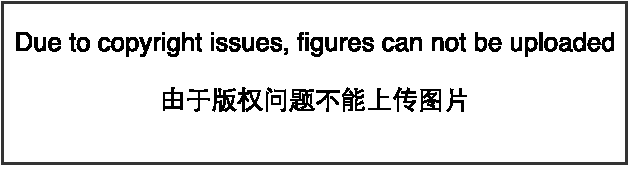
\includegraphics{figure.pdf}}
\else
\centerline{\includegraphics{Chapter1/figures/polar_color}}
\fi
\caption{TODO}
\label{fig:chap1_polar}
\end{figure}

许多\gls{AI}的任务都可以通过提取一个合适的特征集,然后将这些特征提供给简单的\gls{ML}算法来解决。
例如,从声音鉴别说话者的一个有用特征是说话者声道大小的估计。
这个特征为判断说话者是一个男性,女性还是儿童提供了有力线索。

然而,对于许多任务来说,很难知道应该提取哪些特征。
例如,假设我们想编写一个程序来检测照片中的车。
我们知道,汽车有轮子,所以我们可能会想用车轮的存在作为特征。
不幸的是,我们难以准确地从像素值的角度描述一个车轮看起来如何。
车轮具有简单的几何形状,但它的图像可以因为环境而变得很复杂,如落在车轮上的阴影、太阳照亮的车轮的金属零件、汽车的挡泥板或者遮挡的车轮一部分的前景物体,等等。

% -- 3 --

解决这个问题一个途径的是使用\gls{ML}来发现\gls{representation}本身,而不仅仅把表示映射到输出。
这种方法被称为\firstgls{representation_learning}。
学习到的表示往往获得比手动设计的表示更好的性能。
并且它们只需最少的人工干预, 就能让\glssymbol{AI}系统迅速适应新的任务。
\gls{representation_learning}算法只需几分钟就可以为简单的任务发现一个很好的特征集,对于复杂任务则需要几小时到几个月。
手动为一个复杂的任务设计特征需要耗费大量的人工时间和精力;甚至需要花费整个社群研究人员几十年时间。

一个\gls{representation_learning}算法的典型例子是\firstgls{AE}。
\gls{AE}是组合了将输入转换到不同表示\firstgls{encoder}函数和将新的表示转回原来形式的\firstgls{decoder}函数。 
\gls{AE}的训练目标是,输入经过\gls{encoder}和\gls{decoder}之后尽可能多的保留信息,同时希望新的\gls{representation}有各种好的属性。不同种类的\gls{AE}的目标是实现不同种类的属性。

当设计特征或学习特征的算法时,我们的目标通常是分离出能解释观察数据的\textbf{变化因素}(factors of variation)。
在此背景下,``因素''这个词仅指代的影响不同来源;因素通常不是乘性组合。
这些因素通常是不能被直接观察到的量。
相反,他们可能是现实世界中观察不到的物体或者不可观测的力,但影响能观测到的量。
他们还存在于人类的思维构造中,为了给观察到的数据提供有用的简化解释或推断原因。
它们可以被看作帮助我们了解富有变化的数据的概念或者抽象。
当分析语音记录时,变化的因素包括说话者的年龄、性别、他们的口音和他们正在说的词语。
当分析汽车的图像时,变化的因素包括汽车的位置、它的颜色、太阳的角度和亮度。

% -- 4 --

在许多现实世界的\gls{AI}应用困难的一个重要原因是很多因素的变化影响着我们能够观察到的每一个数据。
在夜间,一张图片中红色汽车的单个像素可能是非常接近黑色。
汽车轮廓的形状取决于视角。
大多数应用程序需要我们\emph{理清}变化的因素并丢弃我们不关心的因素。

当然,从原始数据中提取这样的高层次、抽象的特征是非常困难的。
许多这样的变化因素,诸如说话者的口音,只能对数据进行复杂的、接近人类水平的理解来确定。
它几乎与获得原来问题的表示一样困难,乍一看,\gls{representation_learning}似乎并不能帮助我们。

\firstgls{DL}通过其它较简单的表示来表达复杂表示,解决了\gls{representation_learning}中核心问题。

\gls{DL}让计算机通过较简单概念构建复杂的概念。
图\ref{fig:chap1_deep_learning}显示了\gls{DL}系统通过组合较简单的概念,例如转角和轮廓,转而定义边缘来表示图像中一个人的概念。
\begin{figure}[!htb]
\ifOpenSource
\centerline{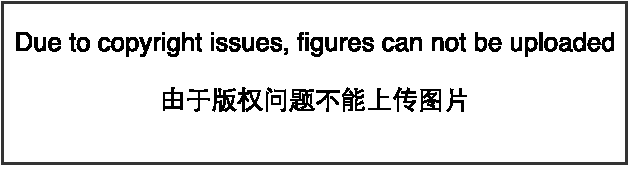
\includegraphics{figure.pdf}}
\else
\centerline{\includegraphics{Chapter1/figures/deep_learning}}
\fi
\caption{TODO}
\label{fig:chap1_deep_learning}
\end{figure}
\gls{DL}模型的典型例子是前馈深度网络或\firstacr{MLP}。
\gls{MLP}仅仅是一个将一组输入值映射到输出的数学函数。
该函数由许多较简单的函数组合而构成。
我们可以认为每个应用具有不同的数学函数,并为输入提供新的表示。

学习数据的正确表示的想法是解释\gls{DL}的一个观点。
另一个观点是深度允许计算机学习一个多步骤的计算机程序。
表示的每一层可以被认为是并行执行另一组指令后计算机的存储器状态。
更深的网络可以按顺序执行更多的指令。
顺序指令提供了极大的能力,因为后面的指令可以参考早期指令的结果。
根据\gls{DL}这个观点,一层的激活函数没有必要对解释输入变化的因素进行编码。
\gls{representation}还存储着协助程序执行的状态信息,使输入更加有意义。
这里的状态信息是类似于传统计算机程序中的计数器或指针。
它与具体的输入内容无关,但有助于模型组织其处理过程。

% -- 6 --

主要有两种测量模型深度的方式。
第一观点是基于评估架构所需执行的顺序指令的数目。
我们可以认为这是描述每个给定输入后,计算模型输出的流程图的最长路径。
正如两个等价的计算机程序根据不同的语言将具有不同的长度,相同的函数可以被绘制为具有不同深度的流程图,这取决于我们允许使用的单一步骤的函数。
图\ref{fig:chap1_language}说明了语言的选择怎样给相同的架构两个不同的衡量。
\begin{figure}[!htb]
\ifOpenSource
\centerline{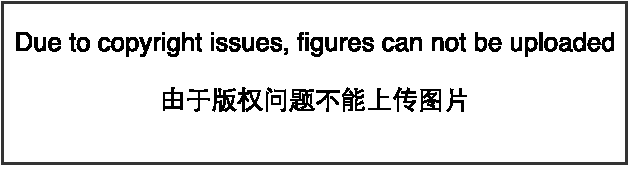
\includegraphics{figure.pdf}}
\else
\centerline{\includegraphics{Chapter1/figures/language}}
\fi
\caption{TODO}
\label{fig:chap1_language}
\end{figure}

另一种是在深度概率模型中使用的方法,不是将计算图的深度视为模型深度,而是将描述概念如何彼此相关的图的深度视为模型深度。
在这种情况下,计算每个概念表示的计算流程图的深度可能比概念本身的图更深。
这是因为系统对较简单概念的理解可以在给出更复杂概念的信息后进一步细化。
例如,一个\glssymbol{AI}系统观察一张其中一只眼睛在阴影中的脸部图像,最初可能只看到一只眼睛。
当检测到的脸部的存在后,它可以推断的第二只眼睛也可能是存在的。
在这种情况下,概念的图仅包括两层——关于眼睛的层和关于脸的层,但是,如果我们根据每个概念给出的其它$n$次估计进行改进,计算的图将包括$2n$个层。

% -- 7 --

由于并不总是清楚计算图的深度或概率模型图的深度哪一个是最相关的,并且由于不同的人选择不同的最小元素集来构建相应的图,导致架构的深度不存在单一的正确值,就像计算机程序的长度不存在单一的正确值。
也不存在模型多少深才能被修饰为``深''的共识。
<BAD>但是,\gls{DL}可以可靠地被视为比传统机器学习涉及更大量的学到函数或学到概念组合的模型的研究。

总之, 这本书的主题——\gls{DL}是\glssymbol{AI}的途径之一。
具体地讲,它是\gls{ML}的一种,一种允许计算机系统能从经验和数据中得到提高的技术。

我们主张\gls{ML}是构建能在复杂实际环境下运行的\glssymbol{AI}系统的唯一可行方法。
\gls{DL}是一种特定类型的\gls{ML},通过将世界表示为由较简单概念定义复杂概念,从一般抽象到高级抽象的嵌套概念体系获得极大的能力和灵活性。
图\ref{fig:chap1_venn}说明了这些不同的\glssymbol{AI}学科之间的关系。图\ref{fig:chap1_which_part_learned}给出了每个学科如何工作的一个高层次的原理。
\begin{figure}[!hbt]
\ifOpenSource
\centerline{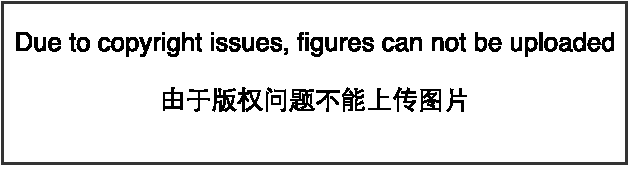
\includegraphics{figure.pdf}}
\else
\centerline{\includegraphics{Chapter1/figures/venn}}
\fi
\caption{TODO}
\label{fig:chap1_venn}
\end{figure}
\begin{figure}[!htb]
\ifOpenSource
\centerline{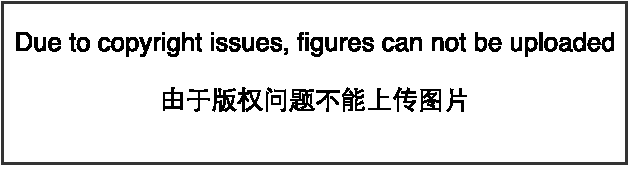
\includegraphics{figure.pdf}}
\else
\centerline{\includegraphics{Chapter1/figures/which_part_learned}}
\fi
\caption{TODO}
\label{fig:chap1_which_part_learned}
\end{figure}

\section{谁应该读这本书?}
\label{sec:who_should_read_this_book}

这本书对各类读者都一定用处的,但我们是基于两个主要目标受众而写的。
其中一个目标受众是学习\gls{ML}的大学生(本科或研究生),包括那些开始了职业生涯的\gls{DL}和\gls{AI}研究者。
另一个目标群体是没有\gls{ML}或统计背景但要迅速在他们的产品或平台开始使用\gls{DL}的软件工程师。
\gls{DL}在许多软件领域都已被证明是有用的,包括计算机视觉、语音和音频处理、自然语言处理、机器人技术、生物信息学和化学、电子游戏、搜索引擎、网络广告和金融。

% -- 8 --

为了最好地适应各类读者,这本书被组织为三个部分。
第一部分介绍了基本的数学工具和\gls{ML}的概念。
<BAD>第二部分介绍了本质上已解决的技术、最成熟的\gls{DL}算法。
第三部分介绍了被广泛认为是深度学习未来研究重点的但更具猜测性的想法。

读者可以随意跳过不感兴趣或与自己背景不相关的部分。
熟悉线性代数、概率和基本\gls{ML}概念的读者可以跳过第一部分,例如,当读者只是想实现一个能工作的系统则不需要阅读超出第二部分的内容。
为了帮助读者选择章节,图\ref{fig:chap1_dependency}展示了这本书的高层组织结构的流程图。
\begin{figure}[!htb]
\ifOpenSource
\centerline{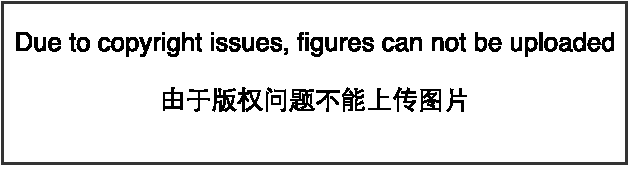
\includegraphics{figure.pdf}}
\else
\centerline{\includegraphics{Chapter1/figures/dependency}}
\fi
\caption{TODO}
\label{fig:chap1_dependency}
\end{figure}

% -- 10 --

我们假设所有读者都具备计算机科学背景。
也假设读者熟悉编程,并且对计算的性能问题、复杂性理论、入门级微积分和一些图论的术语有基本的了解。

\section{深度学习的历史趋势}
\label{sec:historical_trends_in_deep_learning}
通过历史背景了解\gls{DL}是最简单的方式。
我们指出了\gls{DL}的几个关键趋势,而不是提供详细的历史:
\begin{itemize}
 \item \gls{DL}有着悠久而丰富的历史,但伴随着很多反映不同哲学观点名称的尘封而渐渐消逝。
 \item 可用的训练数据的量已经增加,使得\gls{DL}变得更加有用。
 \item 随着时间的推移,针对\gls{DL}的计算机软硬件基础设施都有所改善,\gls{DL}模型的规模也随之增长。
 \item \gls{DL}已经解决日益复杂的应用,并随着时间的推移,精度不断提高。
\end{itemize}

\subsection{神经网络的众多名称和命运变迁}
\label{sec:the_many_names_and_changing_fortunes_of_neural_networks}

我们期待这本书的许多读者都听说过\gls{DL}这一激动人心的新技术,并为一本书提及关于一个新兴领域的``历史''而感到惊讶。
事实上,\gls{DL}的历史可以追溯到20世纪40年代。
\gls{DL}只是\emph{看上去像}一个新的领域,因为在目前流行的前几年它是相对冷门的,同时也因为它被赋予了许多不同的已经消逝的名称,最近才成为所谓的``深度学习''。
这个邻域已经更换了很多名称,反映了不同的研究人员和不同观点的影响。

讲述整个综合性的\gls{DL}历史超出了本书的范围。
然而,一些基本的背景对理解\gls{DL}是有用的。
一般来说,目前为止已经有三次\gls{DL}的发展浪潮:在20世纪40年代到60年代\gls{DL}被称为\firstgls{cybernetics},20世纪80年代到90年代\gls{DL}被誉为\firstgls{connectionism},并于2006年开始,\gls{DL}在当前的名称下开始复苏。
这在图\ref{fig:chap1_cybernetics_connectionism_ngrams_color}中定量给出。
\begin{figure}[!htb]
\ifOpenSource
\centerline{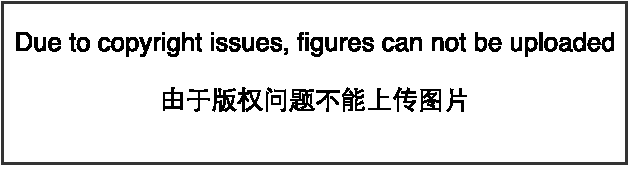
\includegraphics{figure.pdf}}
\else
\centerline{\includegraphics{Chapter1/figures/cybernetics_connectionism_ngrams_color}}
\fi
\caption{TODO}
\label{fig:chap1_cybernetics_connectionism_ngrams_color}
\end{figure}

% -- 12 --

我们现在认识的一些最早的学习算法,旨在模拟生物学习的计算模型,即大脑怎样学习或为什么能学习的模型。
其结果是,已经消逝的\gls{DL}的名称之一——\firstacr{ANN}。
此时\gls{DL}模型对应的观点是他们设计的系统是受生物大脑(无论人类大脑或其他动物的大脑)所启发。
尽管有些\gls{ML}的\gls{NN}有时被用来理解大脑功能\citep{hinton1991lesioning},它们一般都没有被设计成生物功能的真实模型。
\gls{DL}的神经观点受两个主要思想启发的。
一个想法是,大脑这个例子证明智能行为的可能性,因此建立智能概念上的直接途径是逆向大脑背后的计算原,并复制其功能。
另一种看法是,理解大脑和人类智力背后的原则将是非常有趣的,因此\gls{ML}模型除了解决工程应用的能力, 如果能阐明这些基本的科学问题也将会很有用。 

% -- 13 --
  
现代术语``\gls{DL}''超越了目前\gls{ML}模型的神经科学观点。
学习的\emph{多层次组合}这一更普遍的原则更加吸引人,这可以应用于\gls{ML}框架且不必是受神经启发的。
 
 
现代\gls{DL}的最早前身是从神经科学的角度出发的简单线性模型。
这些模型被设计为使用一组$\Sn$个输入$\Sx_1, \dots ,\Sx_n$并将它们与一个输出$\Sy$相关联。 
这些模型将学习一组权重$\Sw_1, \dots, \Sw_n $ 并计算它们的输出$f(\Vx, \Vw) = \Sx_1 \Sw_1 + \dots + \Sx_n \Sw_n$。
这第一波\gls{NN}研究的浪潮被称为\gls{cybernetics},如图\ref{fig:chap1_cybernetics_connectionism_ngrams_color}所示。

\ENNAME{McCulloch-Pitts}神经元\citep{McCulloch43}是脑功能的早期模型。
该线性模型通过测试函数$f(\Vx,\Vw)$的是正还是负来识别两种不同类型的输入。
当然,为了使模型对应于期望的类别定义,需要正确地设置权重。
这些权重可以由操作人员设定。
在20世纪50年代,感知机\citep{Rosenblatt-1956,Rosenblatt-1958}成为第一个能根据了每个类别输入的\gls{example}来学习权重的模型。
约在同一时期,\textbf{自适应线性元件}(ADALINE),简单地返回函数$f(\Vx)$本身的值来预测一个实数\citep{Widrow60},并且还可以学习从数据预测这些数。

这些简单的学习算法大大影响了\gls{ML}的现代景象。
用于调节ADALINE的权重的训练算法是称为\firstgls{SGD}的一种特例。
稍加修改的\gls{SGD}算法仍然是当今\gls{DL}的主要训练算法。

基于感知机和ADALINE中使用的函数$f(\Vx, \Vw)$的模型被称为\firstgls{linear_model}。
这些模型仍然是最广泛使用的\gls{ML}模型,尽管在许多情况下,它们以不同于原始模型的方式进行\emph{训练}。

\gls{linear_model}有很多局限性。
最著名的是,它们无法学习XOR函数,即$f([0,1], \Vw) = 1, f([1,0], \Vw)=1$, 
但是$f([1,1], \Vw)=0, f([0,0],\Vw)= 0$。
在\gls{linear_model}中观察到这些缺陷的评论家开始反对受生物学启发的学习\citep{Minsky69}。
这是\gls{NN}第一次热度较多的下降。

现在,神经科学被视为\gls{DL}研究的一个重要灵感来源,但它已不再是该领域的主要导向。

% -- 14 --

如今神经科学在\gls{DL}研究中的作用被削弱,主要的原因只是我们根本没有足够的关于大脑信息来作为指导。
要获得对大脑实际使用算法的深刻理解,我们需要有能力同时监测(至少是)数千相连神经元的活动。
我们不能够做到这一点,甚至连大脑的最简单、最深入研究的部分我们都还远远没有理解\citep{olshausen:2005}。

神经科学已经给了我们依靠单一\gls{DL}算法解决许多不同任务的理由。
神经学家们发现,如果将雪貂的大脑重新连接,使视觉信号传送到听觉区域,它们可以学会用大脑的听觉处理区域``看''\citep{von2000visual}。
这表明,多数哺乳动物大脑的可能使用单一的算法解决大部分大脑可以解决的不同任务。
这个假设之前,\gls{ML}研究更加分散,研究人员在不同的社区研究自然语言处理、计算机视觉、运动规划和语音识别。
如今,这些应用的社区仍然是独立的,但是\gls{DL}研究小组同时研究许多或甚至所有这些应用领域是很常见的。

我们能够从神经科学得到一些粗略的指南。
仅通过计算单元之间的相互作用而变得智能的基本思想是受大脑启发的。
新认知机\citep{Fukushima80}受哺乳动物视觉系统的结构启发,引入了一个处理图片的强大模型架构,后来成为了现代卷积网络的基础\citep{LeCun98-small},我们将会在\ref{sec:the_neuroscientific_basis_for_convolutional_networks}节看到。
目前大多数\gls{NN}基于称为\firstgls{ReLU}的神经单元模型。
原始认知机\citep{Fukushima75}受我们关于大脑功能知识的启发, 引入了一个更复杂的版本。
简化的现代版基于许多观点进化发展,\citet{Nair-2010}和\citet{Glorot+al-AI-2011-small}援引神经科学作为影响,\citet{Jarrett-ICCV2009}援引更多面向工程的影响。
虽然神经科学是灵感的重要来源,它不需要被视为刚性指导。
我们知道,实际的神经元与现代\gls{ReLU}计算着非常不同函数,但更接近真实神经网络的系统并没有导致\gls{ML}性能的提升。
此外,虽然神经科学已经成功地启发了一些\gls{NN}\emph{架构},但我们还没有足够的了解生物学习的神经科学,因此在训练这些架构时,不能提供给我们很多关于\emph{学习算法}的指导。

媒体报道经常强调\gls{DL}与大脑的相似性。
虽然\gls{DL}研究人员更可能比其他\gls{ML}领域(如核机器或贝叶斯统计工作的研究人员)引用大脑作为影响,人们不应该认为\gls{DL}是对模拟大脑的尝试。
现代\gls{DL}从许多领域获取灵感,特别是应用数学的基本内容如线性代数、概率论、信息论和数值优化。
虽然一些\gls{DL}的研究人员引用神经科学作为灵感的重要来源,但其他学者完全不关心神经科学。

% -- 15 --

值得注意的是,了解大脑是如何在算法层面上工作的尝试是鲜活且发展良好的。
这项尝试主要是被称为``计算神经科学'',并且是独立于\gls{DL}一个领域。
研究人员两个领域之间反复研究是很常见的。
\gls{DL}领域主要是关注如何构建智能的计算机系统,用来解决需要智能才能解决的任务,而计算神经科学领域主要是关注构建大脑如何工作的更精确的模型。

在20世纪80年代,神经网络研究的第二次浪潮在很大程度上是伴随一个被称为\firstgls{connectionism}或\textbf{并行分布处理}运动而出现的\citep{Rumelhart86,mcclelland1995appeal}。
\gls{connectionism}是在认知科学的背景下出现的。
认知科学是理解心智,并结合多个不同层次分析的跨学科方法。
在20世纪80年代初期,大多数认知科学家研究符号推理的模型。
尽管这很流行,符号模型很难解释大脑如何真正使用神经元实现推理功能。 
连接主义者开始研究实际能基于神经实现的认知模型\citep{Touretzky1985},其中很多复苏的想法可以追溯到心理学家\ENNAME{Donald Hebb}在20世纪40年代的工作\citep{Hebb49}。

\gls{connectionism}的中心思想是,当网络将大量简单计算单元连接在一起时可以实现智能行为。
这种见解同样适用于与计算模型中隐层单元类似作用的生物神经系统中的神经元。  

上世纪80年代的\gls{connectionism}运动过程中形成的几个关键概念在今天的\gls{DL}中仍然是非常重要的。

其中一个概念是\firstgls{distributed_representation}\citep{Hinton-et-al-PDP1986}。
这一想法是,系统每个的输入应该由许多特征表示的,并且每个特征应参与许多可能输入的表示。
例如,假设我们有一个能够识别红色、绿色、或蓝色的汽车、卡车和鸟类的视觉系统。
表示这些输入的其中一个方法是将九个可能的组合:红卡车,红汽车,红鸟,绿卡车等等使用单独的神经元或\gls{hidden_unit}激活。
这需要九个不同的神经元,并且每个神经必须独立地学习颜色和对象身份的概念。
改善这种情况的方法之一是使用\gls{distributed_representation},即用三个神经元描述颜色,三个神经元描述对象身份。 
这仅仅需要6个神经元而不是9个,并且描述红色的神经元能够从汽车、卡车和鸟类的图像中学习红色,而不仅仅是从一个特定类别的图像中学习。 
\gls{distributed_representation}的概念是本书的核心,我们将在\ref{chap:representation_learning}章中更加详细地描述。

% -- 16 --

\gls{connectionism}运动的另一个重要成就是反向传播算法的成功运用(训练具有内部表示的深度\gls{NN})和普及\citep{RHW,Lecun-these87}。
这个算法虽然已经黯然失色不再流行,但截至写书之时,仍是训练深度模型的主要方法。

在20世纪90年代,研究人员在使用\gls{NN}进行序列建模的方面取得了重要进展。
\citet{Hochreiter91}和\citet{Bengio1994ITNN}指出了建模长序列的一些根本数学难题,将在\ref{sec:the_challenge_of_longterm_dependencies}节中描述。
\citet{Hochreiter+Schmidhuber-1997}引入\gls{LSTM}(\glssymbol{LSTM})网络来解决这些难题。
如今,\glssymbol{LSTM}在许多序列建模任务中广泛应用,包括Google的许多自然语言处理任务。

\gls{NN}研究的第二次浪潮一直持续到上世纪90年代中期。
基于\gls{NN}等其他\glssymbol{AI}技术的企业开始在寻求投资的同时,做不切实际野心勃勃的主张。
当\glssymbol{AI}研究不能实现这些不合理的期望时,投资者感到失望。
同时,\gls{ML}的其他领域取得进步。
核学习机\citep{Boser92,Cortes95,SchBurSmo99}和图模型\citep{Jordan98}都在很多重要任务上实现了很好的效果。
这两个因素导致了\gls{NN}热度的第二次下降,一直持续到2007年。

在此期间,\gls{NN}持续在某些任务上获得令人印象深刻的表现\citep{LeCun98-small,Bengio-nnlm2001}。
加拿大高级研究所(CIFAR)通过其神经计算和自适应感知(NCAP)研究计划帮助维持\gls{NN}研究。
这个计划统一了由分别由\ENNAME{Geoffrey Hinton},\ENNAME{Yoshua Bengio}和\ENNAME{Yann LeCun}引导的多伦多大学、蒙特利尔大学和纽约大学的\gls{ML}研究小组。
CIFAR NCAP研究计划具有多学科的性质,其中还包括在人类神经科学家和计算机视觉专家。

% -- 17 --

在那个时间点上,普遍认为深度网络被难以训练的。
现在我们知道,从20世纪80年代就存在的算法能工作得非常好,但是直到在2006年前后都没有体现出来。
这个问题可能是单纯的因为计算复杂性太高,而以当时可用的硬件难以进行足够的实验。

神经网络研究的第三次浪潮开始于2006年的突破。
\ENNAME{Geoffrey Hinton}表明名为\gls{DBN}的\gls{NN}可以使用一种称为贪婪逐层训练的策略进行有效地训练\citep{Hinton06},我们将在\ref{sec:greedy_layerwise_unsupervised_pretraining}中更详细地描述。
CIFAR附属的其他研究小组很快表明,同样的策略可以被用来训练许多其他类型的深度网络\citep{Bengio+Lecun-chapter2007-small,ranzato-07},并能系统地帮助提高在测试样例上的泛化能力。
\gls{NN}研究的这一次浪潮普及了``\gls{DL}''这一术语的使用,强调研究人员现在可以训练以前不可能训练的更深的神经网络,并把注意力集中于深度的理论意义\citep{Bengio+Lecun-chapter2007,Delalleau+Bengio-2011-small,Pascanu-et-al-ICLR2014,Montufar-et-al-NIPS2014}。
此时,深度\gls{NN}已经优于与之竞争的基于其他\gls{ML}技术以及手工设计函数的\glssymbol{AI}系统。
神经网络流行的第三次浪潮在写这本书的时候还在继续,尽管深度学习的研究重点在这一段时间内发生了巨大变化。
第三次浪潮开始把重点放在新的无监督学习技术和深度模型从小数据集进行推广的能力,但现在更多的注意点是在更古老的监督学习算法和深度模型充分利用大型标注数据集的能力。

\subsection{与日俱增的数据量}
\label{sec:increasing_dataset_sizes}
人们可能想问,尽管人工\gls{NN}的第一个实验在20世纪50年代就完成了,为什么\gls{DL}直到最近才被认为是关键技术。
自20世纪90年代以来,\gls{DL}就已经成功用于商业应用,但通常被视为是一种艺术而不是一种技术,且只有专家可以使用的艺术,这种观点持续到最近。
确实,要从一个\gls{DL}算法获得良好的性能需要一些技巧。
幸运的是,随着训练数据的增加,所需的技巧正在减少。
目前在复杂的任务达到与人类表现的学习算法,与20世纪80年代努力解决的玩具问题(toy problem)的学习算法几乎是一样的,尽管这些算法训练的模型经历了变革,简化了极深架构的训练。
最重要的新进展是现在我们有了这些算法成功训练所需的资源。
图\ref{fig:chap1_dataset_size_color}展示了基准数据集的大小如何随着时间的推移显着增加。
这种趋势是由社会日益数字化驱动的。
由于我们的活动越来越多发生在计算机上,我们做什么也越来越多地被记录。
我们的计算机越来越多地联网在一起,变得更容易集中管理这些记录,并将它们整理成适于\gls{ML}应用的数据集。
因为``大数据''的时代\gls{ML}要容易得多,因为统计估计的主要负担——观察少量数据以在新数据上泛化——已经减轻。
截至2016年,一个粗略的经验法则是,监督\gls{DL}算法一般在每类给定约5000标注样本情况下可以实现可接受的性能,当至少有1000万标注样本的数据集用于训练时将达到或超过人类表现。
<BAD>在更小的数据集上成功工作是一个重要的研究领域,我们应特别侧重于如何通过无监督或半监督学习充分利用大量的未标注样本。
\begin{figure}[!htb]
\ifOpenSource
\centerline{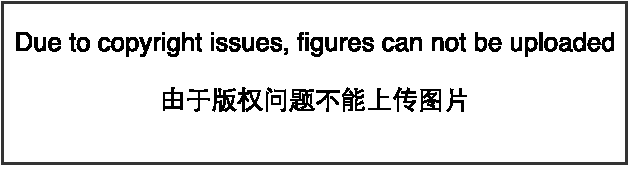
\includegraphics{figure.pdf}}
\else
\centerline{\includegraphics{Chapter1/figures/dataset_size_color}}
\fi
\caption{TODO}
\label{fig:chap1_dataset_size_color}
\end{figure}
\begin{figure}[!htb]
\ifOpenSource
\centerline{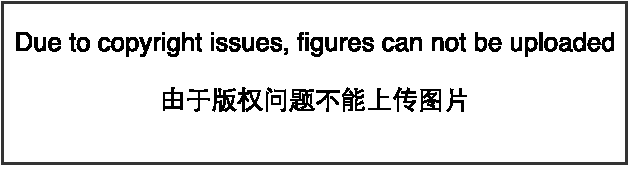
\includegraphics{figure.pdf}}
\else
\centerline{\includegraphics[width=0.8\textwidth]{Chapter1/figures/mnist}}
\fi
\caption{TODO}
\label{fig:chap1_mnist}
\end{figure}

% -- 20 --

\subsection{与日俱增的模型规模}
\label{sec:increasing_model_sizes}

相对20世纪80年代较少的成功,现在\gls{NN}非常成功的另一个重要原因是现在我们拥有的计算资源可以运行更大的模型。
\gls{connectionism}的主要见解之一是,当动物的许多神经元一起工作时会变得聪明。
单独神经元或小集合的神经元不是特别有用。

生物神经元没有连接的特别密集。
如图\ref{fig:chap1_number_of_synapses_color}所示,几十年来,我们的\gls{ML}模型中每个神经元的连接数量甚至与哺乳动物大脑的在同一数量级。
\begin{figure}[!htb]
\ifOpenSource
\centerline{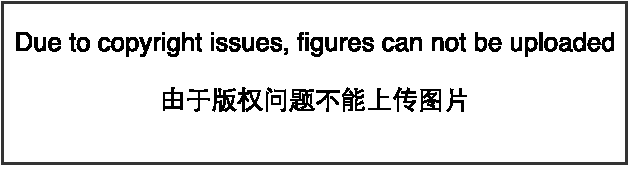
\includegraphics{figure.pdf}}
\else
\centerline{\includegraphics{Chapter1/figures/number_of_synapses_color}}
\fi
\caption{TODO}
\label{fig:chap1_number_of_synapses_color}
\end{figure}

如图\ref{fig:chap1_number_of_neurons_color}所示,就神经元的总数目而言,直到最近\gls{NN}都是惊人的少。
自从引入\gls{hidden_unit}以来,人工\gls{NN}的规模大约每2.4年扩大一倍。
这种增长是由更大内存、更快的计算机和更大的可用数据集驱动的。
较大的网络能够在更复杂的任务中实现更高的精度。
这种趋势看起来将持续数十年。
除非有允许迅速扩展的新技术,否则至少直到21世纪50年代,人工\gls{NN}将才能具备与人脑相同数量级的神经元。
生物神经元表示的函数可能比目前的人工神经元更复杂,因此生物神经网络可能比图中描绘的更大。
\begin{figure}[!htb]
\ifOpenSource
\centerline{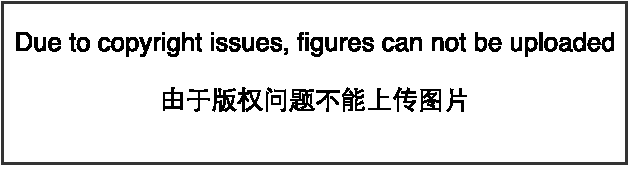
\includegraphics{figure.pdf}}
\else
\centerline{\includegraphics{Chapter1/figures/number_of_neurons_color}}
\fi
\caption{TODO}
\label{fig:chap1_number_of_neurons_color}
\end{figure}


现在回想起来,比一个水蛭的神经元还少的\gls{NN}不能解决复杂的\gls{AI}问题是不足为奇的。
即使是现在从一个计算系统角度来看可能相当大的网络, 实际上比相对原始的脊椎动物如青蛙的神经系统更小。

由于有更快的CPU、通用GPU的到来(在\ref{sec:gpu_implementations}节中讨论)、更快的网络连接和更好的分布式计算的软件基础设施,模型的规模随着时间的推移不断增加是\gls{DL}历史中最重要的趋势之一。
普遍预计这种趋势将很好地持续到未来。

% -- 21 --

\subsection{与日俱增的精度、复杂度和对现实世界的冲击}
\label{sec:increasing_accuracy_complexity_and_real_world_impact}

<BAD>20世纪80年代以来,\gls{DL}一直在提高提供识别精度和预测的能力。
此外,\gls{DL}持续地被成功应用到越来越广泛的应用中去。

最早的深度模型被用来识别裁剪的很合适且非常小的图像中的单个对象\citep{Rumelhart86}。
自那时以来,\gls{NN}可以处理的图像尺寸逐渐增加。
现代对象识别网络能处理丰富的高分辨率照片,并且不要求在被识别的对象附近进行裁剪\citep{Krizhevsky-2012}。
类似地,最早网络只能识别两种对象(或在某些情况下,单一种类的对象的存在与否),而这些现代网络通常识别至少\NUMTEXT{1000}个不同类别的对象。
对象识别中最大的比赛是每年举行的ImageNet大型视觉识别挑战(ILSVRC)。
<BAD>\gls{DL}迅速崛起的一个戏剧性的时刻是卷积网络第一次大幅赢得这一挑战,将最高水准的前5错误率从\NUMTEXT{26.1\%}降到\NUMTEXT{15.3\%}\citep{Krizhevsky-2012},这意味着该卷积网络产生针对每个图像的可能类别的分级列表,尽管\NUMTEXT{15.3\%}的测试样例的正确类别不会出现在此列表中的前5。

此后,深度卷积网络一直能在这些比赛中取胜,截至写书时,\gls{DL}的进步将这个比赛中的前5错误率降到\NUMTEXT{3.6%}, 如图\ref{fig:chap1_imagenet_color}所示。
\begin{figure}[!htb]
\ifOpenSource
\centerline{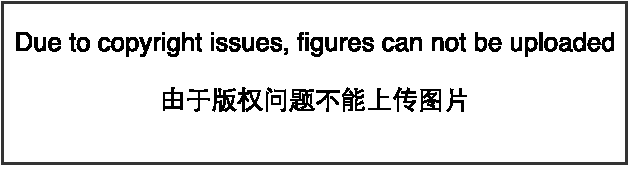
\includegraphics{figure.pdf}}
\else
\centerline{\includegraphics{Chapter1/figures/imagenet_color}}
\fi
\caption{TODO}
\label{fig:chap1_imagenet_color}
\end{figure}

% -- 23 --

\gls{DL}也对语音识别产生了巨大影响。
语音识别在20世纪90年代提高后,直到约2000年都停滞不前。
\gls{DL}的引入\citep{dahl2010phonerec,Deng-2010,Seide2011,Hinton-et-al-2012}导致语音识别错误率的陡然下降,有些错误率甚至降低了一半。 
我们将在\ref{sec:speech_recognition}节更详细地探讨这个历史。

深度网络在行人检测和图像分割中也有引人注目的成功\citep{sermanet-cvpr-13,Farabet-et-al-2013,couprie-iclr-13},在交通标志分类上取得了超越人类的表现\citep{Ciresan-et-al-2012}。

在深度网络的规模和的精度有所提高的同时,它们可以解决的任务也日益复杂。
\citet{Goodfellow+et+al-ICLR2014a}表明,\gls{NN}可以学习输出描述图像的整个字符序列,而不是仅仅识别单个对象。
此前,人们普遍认为,这种学习需要对序列中的单个元素进行标注\citep{Gulcehre+Bengio-arxiv-2013}。
\gls{RNN},如之前提到的\glssymbol{LSTM}序列模型,现在用于建模序列和其他序列之间的关系,而不是仅仅固定输入之间的关系。
这个序列到序列的学习似乎处于另一个应用演进的浪尖:机器翻译\citep{Sutskever-et-al-NIPS2014,Bahdanau-et-al-ICLR2015-small}。

% -- 24 --

日益复杂的趋势已将其推向逻辑结论,即神经图灵机\citep{Graves-et-al-arxiv2014}的引入,它能学习读取存储单元和向存储单元写入任意内容。
这样的\gls{NN}可以从期望行为的\gls{example}中学习简单的程序。
例如,从杂乱和排好序的\gls{example}中学习对一系列数进行排序。
这种自我编程技术正处于起步阶段,但原则上未来可以适用于几乎所有的任务。


\gls{DL}的另一个冠军成就是在\firstgls{RL}领域的扩展。
在\gls{RL}的背景下,一个自主体必须通过试错来学习执行任务,而无需人类操作者的任何指导。
DeepMind表明,基于\gls{DL}的\gls{RL}系统能够学会玩Atari视频游戏,并在多种任务中可与人类匹敌\citep{Mnih-et-al-2015}。
\gls{DL}也显著改善了机器人\gls{RL}的性能\citep{finn2015learning}。

许多\gls{DL}应用都是高利润的。现在\gls{DL}被许多顶级的技术公司使用,包括Google、Microsoft、Facebook、IBM、Baidu、Apple、Adobe、Netflix、NVIDIA和NEC。

\gls{DL}的进步也严重依赖于软件基础架构的进展。
软件库如Theano\citep{bergstra+al:2010-scipy,Bastien-2012}、PyLearn2\citep{pylearn2_arxiv_2013}、Torch\citep{Torch-2011}、DistBelief\citep{Dean-et-al-NIPS2012}、Caffe\citep{Jia13caffe}、MXNet\citep{chen2015mxnet}和TensorFlow\citep{tensorflow}都能支持重要的研究项目或商业产品。

\gls{DL}也为其他科学做出了贡献。
识别对象的现代卷积网络提供给神经科学家可以研究的视觉处理模型\citep{dicarlo-tutorial-2013}。
\gls{DL}也为处理海量数据、在科学领域作出的有效预测提供了非常有用的工具。
它已成功地用于预测分子如何相互作用,这能帮助制药公司设计新的药物\citep{Dahl-et-al-arxiv2014}、搜索的亚原子粒子\citep{baldi2014searching}和自动解析用于构建人脑三维图的显微镜图像\citep{knowlesdeep}。
我们期待\gls{DL}未来出现在越来越多的科学领域。

% -- 25 --

总之,\gls{DL}是\gls{ML}的一种方法, 过去几十年的发展中,它深深地吸收了我们关于人脑、统计学与应用数学的知识。
近年来,\gls{DL}的普及性和实用性有了极大的发展,这在很大程度上得益于更强大的计算机、更大的数据集和能够训练更深网络的技术。
未来几年充满了进一步提高\gls{DL}并将它带到新领域挑战和机遇。

% -- 26 --

%% Translator: Yujun Li 
\chapter{线性代数}
\label{chap:linear_algebra}

线性代数作为数学的一个分支,广泛用于科学和工程中。
然而,因为线性代数主要是面向连续数学,而非离散数学,所以很多计算机科学家很少接触它。
掌握好线性代数对于理解和从事机器学习算法相关工作是很有必要的,尤其对于深度学习而言。
因此,在我们开始介绍深度学习之前,我们集中探讨一些必备的线性代数知识。


如果你已经很熟悉线性代数,那么你可以轻松地跳过本章。
如果你先前接触过本章的内容,但是需要一份索引表来回顾一些重要公式,那么我们推荐\emph{The Matrix Cookbook} \citep{matrix-cookbook}。
如果你没有接触过线性代数,那么本章将告诉你本书所需的线性代数知识,不过我们仍然非常建议你参考其他专注于讲解线性代数的资料,例如\cite{shilov1977linear}。
最后,本章跳过了很多重要但是对于理解深度学习非必需的线性代数知识。




\section{标量,向量,矩阵和张量}
\label{sec:scalars_vectors_matrices_and_tensors}

线性代数的学习将会涉及以下几个数学对象:
\begin{itemize}
    \item \firstgls{scalar}:一个标量就是一个单独的数,不同于线性代数中涉及到多个数的大多数对象。
    我们会用斜体表示标量。标量通常会被赋予小写的变量名称。
    当我们介绍标量时,会明确它们是哪种类型的数。
    比如,在定义实数标量时,我们可能会说“让$\Ss \in \SetR$表示一条线的斜率”;在定义自然数标量时,我们可能会说“让$\Sn\in\SetN$表示元素的数目”。

% -- 29 --

    \item \firstgls{vector}:一个向量是一列数。
    这些数是有序排布的。
    通过次序中的\gls{index},我们可以确定每个单独的数。
    通常我们会赋予向量粗体的小写名称,比如$\Vx$。
    向量中的元素会通过带脚标的斜体来表示。
    向量$\Vx$的第一个元素是$\Sx_1$,第二个元素是$\Sx_2$,等等。
    我们也会注明存储在向量中的元素是什么类型的。
    如果每个元素都属于$\SetR$,并且该向量有$\Sn$个元素,那么该向量属于实数集$\SetR$笛卡尔乘积$\Sn$次,表示为$\SetR^n$。
    当我们需要明确表示向量中的元素时,我们会将元素排列成一个方括号包围的纵柱:
    \begin{equation}
        \Vx=\begin{bmatrix} \Sx_1   \\  
                            \Sx_2   \\ 
                            \vdots  \\ 
                            \Sx_n 
                \end{bmatrix}
    \end{equation}
    我们可以把向量看作空间中的点,每个元素是不同的坐标轴上的坐标。
    
    有时我们需要指定向量中某个集合的元素。
    在这种情况下,我们定义一个包含这些\gls{index}的集合,然后将该集合写在脚标处。
    比如,指定$\Sx_1$,$\Sx_3$和$\Sx_6$,我们定义集合$S=\{1,3,6\}$,然后写作$\Vx_S$。我
    们用符号$-$表示集合的补集中的\gls{index}。
    比如$\Vx_{-1}$表示$\Vx$中除$\Sx_1$外的所有元素,$x_S$表示$\Vs$中除$\Sx_1$,$\Sx_3$,$\Sx_6$外所有元素构成的向量。

    \item \firstgls{matrix}:矩阵是二维数组,其中的每一个元素被两个\gls{index}而非一个所确定。
    我们通常会赋予矩阵粗体的大写变量名称,比如$\MA$。
    如果一个实数矩阵高度为$m$,宽度为$n$,那么我们说$\MA\in \SetR^{m\times n}$。
    我们在表示矩阵中的元素时,通常使用其名称以不加粗的斜体形式,\gls{index}用逗号间隔。
    比如,$\SA_{1,1}$表示$\MA$左上的元素,$\MA_{m,n}$表示$\MA$右下的元素。
    我们表示垂直坐标$\Si$中的所有元素时,用“:”来表示水平坐标。
    比如,$\MA_{i,:}$表示$\MA$中垂直坐标$i$上的一横排元素。
    这也被称为$\MA$的第$i$\firstgls{column}。
    同样地,$\MA_{:,i}$表示$\MA$的第$i$\firstgls{row}。
    当我们需要明确表示矩阵中的元素时,我们将它们写在用方括号包围起来的数组中:
    \begin{equation}
        \begin{bmatrix}
            A_{1,1} & A_{1,2} \\
            A_{2,1} & A_{2,2} \\
        \end{bmatrix}
    \end{equation}
    有时我们需要矩阵值表达式的\gls{index},而不是单个元素。
    在这种情况下,我们在表达式后面接下标,但不需要写作小写字母。
    比如,$f(\MA)_{i,j}$表示函数$f$作用在$\MA$上输出的矩阵的第$(i,j)$个元素。

% -- 30 --

    \item \firstgls{tensor}:在某些情况下,我们会讨论不只两维坐标的数组。
    一般地,一组数组中的元素分布在若干维坐标的规则网格中,我们将其称之为张量。
    我们使用这种字体$\TSA$来表示张量“A”。
    张量$\TSA$中坐标为$(i,j,k)$的元素记作$\textsf{\emph{A}}_{i,j,k}$。
\end{itemize}


\firstgls{transpose}是矩阵的重要操作之一。
矩阵的转置是以对角线为轴的镜像,这条从左上角到右下角的对角线称为\firstgls{main_diagonal}。
图\ref{fig:chap2_transpose}显示了这个操作。
我们将矩阵$\MA$的转置表示为$\MA^\top$,定义如下
\begin{equation}
(\MA^\top)_{i,j}= \SA_{j,i}
\end{equation}

\begin{figure}[!htb]
\ifOpenSource
\centerline{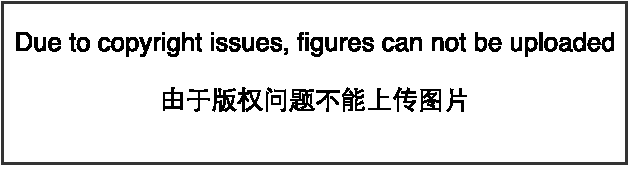
\includegraphics{figure.pdf}}
\else
\centerline{\includegraphics{Chapter2/figures/transpose}}
\fi
\caption{TODO}
\label{fig:chap2_transpose}
\end{figure}

向量可以被看作是只有一列的矩阵。
对应地,向量的转置可以被看作是只有一行的矩阵。
有时,我们将向量表示成行矩阵的转置,写在行中,然后使用转置将其变为标准的列向量,比如$\Vx=[\Sx_1, \Sx_2, \Sx_3]^\top$.


标量可以看作是只有一个元素的矩阵。
因此,标量的转置等于它本身,$\Sa=\Sa^\top$。

% -- 31 --

只要矩阵的形状一样,我们可以把两个矩阵相加。
两个矩阵相加是指对应位置的元素相加,比如$\MC=\MA+\MB$,其中$\SC_{i,j}= \SA_{i,j}+\SB_{i,j}$。


标量和矩阵相乘,或是和矩阵相加时,我们将其与矩阵的每个元素相乘或相加,比如$\MD = \Sa \cdot \MB + \Sc$,其中$\SD_{i,j} = \Sa\cdot  \SB_{i,j} + \Sc$。


在深度学习中,我们也使用一些不那么常规的符号。
我们允许矩阵和向量相加,产生另一个矩阵:$\MC=\MA + \Vb$,其中$\SC_{i,j}= \SA_{i,j} + \Sb_{j}$。
换言之,向量$\Vb$和矩阵$\MA$的每一行相加。
这个速记方法使我们无需在加法操作前定义复制向量$\Vb$到矩阵的每一行。
这种隐式的拷贝向量$\Vb$到很多地方,被称之为\firstgls{broadcasting}。




\section{矩阵和向量相乘}
\label{sec:multiplying_matrices_and_vectors}

矩阵乘法是矩阵运算中最重要的操作之一。
两个矩阵$\MA$和$\MB$的\firstgls{matrix_product}是第三个矩阵$\MC$。
为了使得乘法定义良好,矩阵$\MA$的列数必须和矩阵$\MB$的行数相等。
如果矩阵$\MA$的形状是$\Sm \times \Sn$,矩阵$\MB$的形状是$\Sn\times \Sp$,那么矩阵$\MC$的形状是$\Sm\times \Sp$。
矩阵乘积可以作用于两个或多个并在一起的矩阵,即
\begin{equation}
    \MC=\MA\MB。
\end{equation}


具体地,该乘法操作定义为
\begin{equation}
    \SC_{i,j}=\sum_k \SA_{i,k} \SB_{k,j}
\end{equation}


需要注意的是,两个矩阵的标准乘积\emph{不是}指两个矩阵中对应元素的乘积。
不过,那样的矩阵操作确实是存在的,称之为\firstgls{element_wise_product}或者\firstgls{hadamard_product},表示为$\MA\odot\MB$。


两个相同维数的向量$\Vx$和$\Vy$的\firstgls{dot_product}可看作是矩阵乘积$\Vx^\top\Vy$。
我们可以把矩阵乘积$\MC=\MA\MB$中计算$\SC_{i,j}$的步骤看作是$\MA$的第$\Si$行和$\MB$的第$\Sj$列之间的\gls{dot_product}。


矩阵乘积运算有许多有用的性质,从而使矩阵的数学分析更加方便。
比如,矩阵乘积服从分配律:


\begin{equation}
    \MA(\MB+\MC)=\MA\MB +\MA\MC
\end{equation}


矩阵乘积也服从结合律:


\begin{equation}
\MA(\MB\MC)=(\MA\MB)\MC
\end{equation}


% -- 32 --


不同于标量乘积,矩阵乘积并不满足交换律($\MA\MB=\MB\MA$的情况并非总是满足)。
然而,两个向量的\firstgls{dot_product}满足交换律:


\begin{equation}
\Vx^\top\Vy=\Vy^\top\Vx
\end{equation}


矩阵乘积的转置有着简单的形式:


\begin{equation}
(\MA\MB)^\top=\MB^\top\MA^\top
\end{equation}


利用向量乘积是标量,标量转置是自身的事实,我们可以证明式2.8:
\begin{equation}
    \Vx^\top \Vy = \left(\Vx^\top \Vy \right)^\top = \Vy^\top \Vx
\end{equation}


由于本书的重点不是线性代数,我们并不试图展示矩阵乘积的所有重要性质,但读者应该知道矩阵乘积还有很多有用的性质。


现在我们已经知道了足够多的线性代数符号,可以表达下列线性方程组:


\begin{equation}
\MA\Vx=\Vb
\end{equation}
其中$\MA\in \SetR^{m\times n}$是一个已知矩阵,$\Vb$是一个已知向量,$\Vx$是一个我们要求解的未知向量。
向量$\Vx$的每一个元素$\Sx_i$都是未知的。
矩阵$\MA$的每一行和$\Vb$中对应的元素构成另一个约束。
我们可以把式2.11重写为
\begin{equation}\MA_{1,:}\Vx=b_1 \end{equation}
\begin{equation}\MA_{2,:}\Vx=b_2 \end{equation}
\begin{equation}\cdots \end{equation}
\begin{equation}\MA_{m,:}\Vx=b_m \end{equation}
或者,更明确地,写作
\begin{equation}
    \MA_{1,1}x_1+\MA_{1,2}x_2+\cdots \MA_{1,n}x_n = b_1
\end{equation}
\begin{equation}
    \MA_{2,1}x_1+\MA_{2,2}x_2+\cdots \MA_{2,n}x_n = b_2
\end{equation}
\begin{equation}
    \cdots
\end{equation}
\begin{equation}
    \MA_{m,1}x_1+\MA_{m,2}x_2+\cdots \MA_{m,n}x_n = b_m
\end{equation}


矩阵向量乘积符号为这种形式的等式提供了更紧凑的表示。



% -- 33 --


\section{单位矩阵和逆矩阵}
\label{sec:identity_and_inverse_atrices}


线性代数提供了被称为\firstgls{matrix_inverse}的强大工具,使我们能够解析地求解式2.11中的多值$\MA$。


为了描述矩阵逆,我们首先需要定义\firstgls{identity_matrix}的概念。
任意向量和单位矩阵相乘,都不会改变。
我们将保持$\Sn$维向量不变的单位矩阵记作为$\MI_{\Sn}$。
形式上,$\MI_{\Sn}\in \SetR^{\Sn\times \Sn}$,
\begin{equation}
    \forall \Vx \SetR^{\Sn} \in \MI_{\Sn}, \MI_{\Sn} \Vx = \Vx 
\end{equation}


单位矩阵的结构很简单:所有沿主对角线的元素都是$1$,而所有其他位置的元素都是$0$。
如图2.2所示。


矩阵$\MA$的\firstgls{matrix_inverse}被记作$\MA^{-1}$,被定义为如下的矩阵
\begin{equation} \MA^{-1}\MA = \MI_{\Sn} \end{equation}
现在我们可以通过如果以下步骤求解式2.11:
\begin{equation}\MA\Vx=\Vb \end{equation}
\begin{equation} \MA^{-1}\MA\Vx = \MA^{-1}\Vb \end{equation}
\begin{equation} \MI_{\Sn} \Vx=\MA^{-1}\Vb \end{equation}
\begin{equation} \Vx=\MA{-1}\Vb \end{equation}


当然,这取决于能否找到一个逆矩阵$\MA^{-1}$。
在接下来的章节,我们讨论逆矩阵$\MA^{-1}$存在的条件。


当逆矩阵$\MA^{-1}$存在时,有几种不同的算法都能找到它的闭解形式。
理论上,相同的逆矩阵可用于多次求解不同向量$\Vb$的方程。
然而,逆矩阵$\MA^{-1}$主要有用于理论工具,不会真的在大多数实际软件应用程序中使用。
这是因为逆矩阵$\MA^{-1}$在数字计算机上只能表现出有限的精度,有效使用向量$\Vb$的算法通常可以得到更精确的$\Vx$。



% -- 34 --


\section{线性相关和生成子空间}
\label{sec:linear_dependence_and_span}

如果逆矩阵$\MA^{-1}$存在,那么式2.11肯定对于每一个向量$\Vb$恰好存在一个解。
对系统方程而言,对于某些$\Vb$的值,有可能不存在解,或者存在无限多个解。
然而,存在多于一个解但是少于无穷多个解的情况是不可能发生的;因为如果$\Vx$和$\Vy$都是某系统方程的解,则
\begin{equation}
\Vz=\alpha \Vx + (1-\alpha) \Vy
\end{equation}
(其中$\alpha$取任意实数)也是该系统方程的解。


分析方程有多少个解,我们可以将$\MA$的列向量看作是从\firstgls{origin}(元素都是零的向量)出发的不同方向,确定有多少种方法可以到达向量$\Vb$。
在这个观点中,向量$\Vx$中的每个元素表示我们应该沿着这些方向走多远,即$\Sx_{\Si}$表示我们需要沿着第$\Si$个向量的方向走多远:
\begin{equation}
\MA \Vx = \sum_i x_i \MA_{:,i}
\end{equation}
一般来说,这种操作被称为\firstgls{linear_combination}。
形式上,某个集合中向量的线性组合,是指每个向量乘以对应系数之后的和,即:
\begin{equation}
    \sum_i \Sc_i \Vv^{(i)}
\end{equation}
一组向量的\firstgls{span}是原始向量线性组合后所能抵达的点的集合。


确定$\MA\Vx=\Vb$是否有解相当于确定向量$\Vb$是否在$\MA$列向量的生成子空间中。
这个特殊的生成子空间被称为$\MA$的\firstgls{column_space}或者$\MA$的\firstgls{range}。


为了让方程$\MA \Vx=\Vb$对于任意的向量$\Vb$都有解的话,我们需要要求$\MA$的列空间构成整个$\SetR^{\Sm}$。
如果$\SetR^m$中的某个点不在$\MA$的列空间中,那么该点对应的$\Vb$会使得该方程没有解。
矩阵$\MA$的列空间是整个$\SetR^m$的要求,意味着$\MA$至少有$m$列,即$n\geq m$。
否则,$\MA$列空间的维数会小于$m$。
例如,假设$\MA$是一个$3\times 2$的矩阵。
目标$b$是$3$维的,但是$x$只有$2$维。
所以无论如何修改$x$的值,也只能描绘出$\SetR^3$空间中的二维平面。
当且仅当向量$\Vb$在该二维平面中时,该方程有解。



% -- 35 --


不等式$n\geq m$仅是方程对每一点都有解的必要条件。
这不是一个充分条件,因为有些列向量可能是冗余的。
假设有一个$\SetR^{2\times 2}$中的矩阵,它的两个列向量是相同的。
那么它的列空间和它的一个列向量作为矩阵的列空间是一样的。
换言之,虽然该矩阵有$2$列,但是它的列空间仍然只是一条线,不能涵盖整个$\SetR^2$。


正式地,这种冗余被称为\firstgls{linear_depend}。
如果一组向量中的任意一个向量都不能表示成其他向量的线性组合,那么这组向量被称之为线性无关(linearly independent)。
如果某个向量是一组向量中某些向量的线性组合,那么我们将这个向量加入到这组向量后不会增加这组向量的生成空间。
这意味着,如果一个矩阵的列空间涵盖整个$\SetR^m$,那么该矩阵必须包含至少一组$m$个线性无关的向量。
这是式2.11对于每一个向量$\Vb$的取值都有解的充足条件。
值得注意的是,这个条件是说该向量集恰好有$m$个线性无关的列向量,而不是至少$m$个。
不存在一个$m$维向量的集合具有多于$m$个彼此线性不相关的列向量,但是一个有多于$m$个列向量的矩阵却有可能拥有不止一个大小为$m$的线性无关向量集。


要想使矩阵可逆,我们还需要保证式2.11对于每一个$\Vb$值至多有一个解。
为此,我们需要确保该矩阵至多有$m$个列向量。
否则,该方程会有不止一个解。


综上所述,这意味着该矩阵必须是一个\firstgls{square},即$m=n$,并且所有列向量都是线性无关的。一个列向量线性相关的方阵被称之为\firstgls{singular}。


如果矩阵$A$不是一个方阵或者是一个奇异的方阵,该方程仍然可能有解。
但是我们不能使用逆矩阵去求解。


到目前为止,我们已经讨论了逆矩阵左乘。我们也可以定义逆矩阵右乘:
\begin{equation}
\MA\MA^{-1}=\MI
\end{equation}
对于方阵而言,它的左逆和右逆是相等的。




\section{范数}
\label{sec:norms}

有时我们需要衡量一个向量的大小。
在机器学习中,我们经常使用被称为\firstgls{norm}的函数衡量矩阵大小。
形式上,$L^p$范数如下
\begin{equation}
    \norm{\Vx}_p = \left( \sum_i |x_i|^p \right)^{\frac{1}{p}}
\end{equation}
其中$p\in \SetR$,$p\geq 1$。



% -- 36 --


范数(包括$L^p$范数)是将向量映射到非负值的函数。
直观上来说,向量$\Vx$的范数是衡量从原点到点$\Vx$的距离。
更严格地说,范数是满足下列性质的任意函数:
\begin{itemize}
\item $f(\Vx) = 0 \Rightarrow \Vx = \mathbf{0}$ 
\item $f(\Vx + \Vy) \leq f(\Vx) + f(\Vy)$ (\firstgls{triangle_inequality})
\item $\forall \alpha \in \SetR$, $f(\alpha \Vx) = |\alpha| f(\Vx)$
\end{itemize}


当$p=2$时,$L^2$被称为\firstgls{euclidean_norm}。
它表示从原点出发到向量$\Vx$确定的点的欧几里得距离。
$L^2$范数十分频繁地出现在机器学习中,它经常被简化表示为$\norm{x}$,略去了下标$2$。
平方$L^2$范数也经常被用来衡量向量的大小,可以简单地t通过\gls{dot_product}$\Vx^\top\Vx$计算。


平方$L^2$范数在数学和计算上都比$L^2$范数本身更方便。
例如,平方$L^2$范数对$\Vx$中每个元素的导数只取决于对应的元素,而$L^2$范数对每个元素的导数却和整个向量相关。
但是在很多情况下,平方$L^2$范数也可能不受欢迎,因为它在原点附近增长得十分缓慢。
在某些机器学习应用中,区分元素值恰好是零还是非零小值是很重要的。
在这些情况下,我们更倾向于使用在各个位置斜率相同,同时保持简单的数学形式的函数:$L^1$范数。
$L^1$范数可以简化如下:
\begin{equation}
    \norm{\Vx}_1 = \sum_i  |x_i|
\end{equation}
当机器学习问题中零和非零元素之间的差异非常重要时,通常会使用$L^1$范数。
每当$\Vx$中某个元素从$0$增加了$\epsilon$,对应的$L^1$范数增加$\epsilon$。


有时候我们会通过统计向量中非零元素的个数来衡量向量的大小。
有些作者将这种函数称之为“$L^0$范数”,但是这个术语在数学意义上是不对的。
向量的非零元素的数目不是范数,因为对标量放缩$\alpha$倍不会改变该向量非零的数目。
因此,$L^1$范数经常被用作表示非零元素数目的替代。



% -- 37 --


另外一个经常在机器学习中出现的范数是$L^\infty$范数,也被称为\firstgls{max_norm}。
这个范数表示向量中具有最大幅度的元素的绝对值:
\begin{equation}
    \norm{\Vx}^\infty = \max_i |x_i|
\end{equation}


有时候我们可能也需要衡量矩阵的大小。
在深度学习中,最常见的做法是使用\firstgls{frobenius_norm},
\begin{equation}
    \norm{A}_F = \sqrt{\sum_{i,j} A_{i,j}^2}
\end{equation}
类似于向量的$L^2$范数。


两个向量的\firstgls{dot_product}可以用范数来表示。
具体地,
\begin{equation}
    \Vx^\top\Vy = \norm{\Vx}_2\norm{\Vy}_2 \cos \theta
\end{equation}
其中$\theta$表示$\Vx$和$\Vy$之间的夹角。




\section{特殊类型的矩阵和向量}
\label{sec:special_kinds_of_matrices_and_vectors}

有些特殊类型的矩阵和向量是特别有用的。


\firstgls{diagonal_matrix}只在主对角线上含有非零元素,其它位置都是零。
形式上,矩阵$\MD$是对角矩阵,当且仅当对于所有的$i\neq j$,$\SD_{i,j}=0$。
我们已经看到过一个对角矩阵:单位矩阵,对角元素全部是$1$。
我们用$\text{diag}(\Vv)$表示一个对角元素由向量$\Vv$中元素给定的对角方阵。
对角矩阵受到关注,部分原因是对角矩阵的乘法计算很高效。
计算乘法$\text{diag}(\Vv)\Vx$,我们只需要将$\Vx$中的每个元素$x_i$放大$v_i$倍。
换言之,$\text{diag}(\Vv)\Vx=\Vv \odot \Vx$。
计算对角矩阵的逆矩阵也很高效。
对角矩阵的逆矩阵存在,当且仅当对角元素都是非零的,在这种情况下,$\text{diag}(\Vv)^{-1}=\text{diag}([1/v_1,\dots,1/v_n]^\top$。
在很多情况,我们可以根据任意矩阵导出一些通用的机器学习算法;但通过将一些矩阵限制为对角矩阵,我们可以得到计算代价较低的(并且描述语言较少的)算法。


不是所有的对角矩阵都是方阵。
长方形的矩阵也有可能是对角矩阵。
长方形对角矩阵没有逆矩阵,但我们仍然可以很快地计算它们的乘法。
对于一个长方形对角矩阵$\MD$而言,乘法$\MD\Vx$会涉及到$\Vx$中每个元素的放缩,如果$\MD$是瘦长型矩阵,那么在放缩后的向量添加一些零;如果$\MD$是胖长型矩阵,那么放缩后去掉最后一些元素。


% -- 38 --

\firstgls{symmetric}矩阵是任意转置和自己相等的矩阵:
\begin{equation}
    \MA=\MA^\top
\end{equation}
当某些不依赖参数顺序的双参数函数生成元素时,对称矩阵经常会出现。
例如,如果$\MA$一个表示距离的矩阵,$\MA_{i,j}$表示点$i$到点$j$的距离,那么$\MA_{i,j}=\MA_{j,i}$,因为距离函数是对称的。


\firstgls{unit_vector}指的是范数为$1$的向量:
\begin{equation}
\norm{\Vx}=1
\end{equation}


如果$\Vx^\top \Vy = 0$,那么向量$\Vx$和向量$\Vy$互相\firstgls{orthogonal}。
如果两个向量都有非零范数,那么表示这两个向量之间的夹角是$90$度。
在$\SetR^n$中,至多有$n$个范数非零向量互相正交。
如果这些向量不仅互相正交,并且范数都为$1$,那么我们称它们是\firstgls{orthonormal}。


\firstgls{orthogonal_matrix}是指行向量是标准正交的,列向量是标准正交的方阵:
\begin{equation}
    \MA^\top\MA=\MA\MA^\top=\MI
\end{equation}
这意味着 
\begin{equation}
    \MA^{-1}=\MA^\top
\end{equation}
所以正交矩阵受到关注是因为求逆计算代价小。
需要注意正交矩阵的定义。
反直觉地,正交矩阵的行向量不仅是正交的,还是标准正交的。
对于行向量或列向量互相正交但不是标准正交的矩阵没有对应的专有术语。




\section{特征分解}
\label{sec:eigendecomposition}

许多数学对象可以通过将它们分解成多个组成部分,或者找到它们的一些属性而被更好地理解,这些属性是通用的,而不是由我们选择表示它们的方式引起的。

% -- 39 --

例如,整数可以被分解为质数。
我们表示整数$12$的方式取决于我们用十进制还是二进制去表示它,但质因数分解永远是对的$12=2\times 3\times 3$。
从这个表示中我们可以获得一些有用的信息,比如$12$不能被$5$整除,或者$12$的倍数可以被$3$整除。


就像我们可以通过分解质因数来发现一些关于整数的真实性质,我们也可以通过分解矩阵来获取一些矩阵表示成数组元素时不明显的函数性质。


\firstgls{eigendecomposition}是使用最广的矩阵分解之一,即我们将矩阵分解成一组特征向量和特征值。


方阵$\MA$的\firstgls{eigenvector}是指与$\MA$相乘后相当于对该向量进行放缩的非零向量$\Vv$:
\begin{equation}
    \MA\Vv=\lambda \Vv
\end{equation}
标量$\lambda$被称之为这个特征向量对应的\firstgls{eigenvalue}。
(类似地,我们也可以定义\firstgls{left_Svector}$\Vv^\top\MA=\lambda \Vv^\top$,但是通常我们更关注\firstgls{right_Svector})。


如果$\Vv$是$\MA$的特征向量,那么任何放缩后的向量$s\Vv$($s\in \SetR$)也是$\MA$的特征向量。
此外,$s\Vv$和$\Vv$有相同的特征值。
基于这个原因,通常我们只考虑单位特征向量。


假设矩阵$\MA$有$n$个线性无关的特征向量$\{\Vv_1, \dots, \Vv_n\}$,对应着特征值$\{\lambda_1, \dots , \lambda_n \}$。
我们将特征向量连接一个矩阵,使得每一列是一个特征向量:$V=[\Vv_1, \dots , \Vv_n]$.
类似地,我们也可以将特征值连接成一个向量$\Vlambda = [\lambda_1, \dots , \lambda_n]^\top$。
因此$\MA$的\gls{eigendecomposition}可以记作
\begin{equation}
    \MA = \MV \text{diag}(\mathbf{\Vlambda}) \MV^{-1}
\end{equation}


我们已经看到了\emph{构建}具体特定的特征值和特征向量,能够使我们在目标方向上延伸空间。
然而,我们也常常希望将矩阵\firstgls{decompose}成特征值和特征向量。
这样可以帮助我们分析矩阵的特定性质,就像质因数分解有助于我们理解整数。


不是每一个矩阵都可以分解成特征值和特征向量。
在某些情况下,特征分解会涉及到复数,而非实数。
幸运的是,在本书中我们通常只需要探讨一类有简单分解的矩阵。
具体地,每个实对称矩阵都可以分解成实特征向量和实特征值:
\begin{equation}
    \MA = \MQ \VLambda \MQ^\top
\end{equation}
其中$\MQ$是$\MA$的特征向量组成的正交矩阵,$\VLambda$是对角矩阵。
特征值$\Lambda_{i,i}$对应的特征向量是矩阵$\MQ$的第$i$列,记作$\MQ_{:,i}$。
因为$\MQ$是正交矩阵,我们可以将$\MA$看作是沿方向$\Vv^{(i)}$延展$\lambda_i$倍的空间。
如图\ref{fig:chap2_eigen_ellipse}所示。

% -- 40 --

虽然任意一个实对称矩阵$\MA$都有特征分解,但是特征分解可能并不唯一。
如果两个或多个特征向量拥有相同的特征值,那么这组特征向量生成子空间中,任意一组正交向量都是该特征值对应的特征向量。
因此,我们可以使用任意一组正交向量作为$\MQ$的特征向量。
按照惯例,我们通常按降序排列$\VLambda$的条目。
在该约定下,特征分解唯一当且仅当所有的特征值都是唯一的。

\begin{figure}[!htb]
\ifOpenSource
\centerline{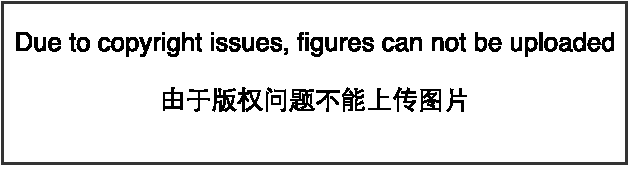
\includegraphics{figure.pdf}}
\else
\centerline{\includegraphics[width=0.8\textwidth]{Chapter2/figures/eigen_ellipse_color}}
\fi
\caption{TODO}
\label{fig:chap2_eigen_ellipse}
\end{figure}

% -- 41 --


矩阵的特征分解给了我们很多关于矩阵的有用信息。
矩阵是奇异的当且仅当含有零特征值。
实对称矩阵的特征分解也可以用于优化二次方程$f(\Vx) = \Vx^\top \MA \Vx$,其中限制$\norm{\Vx}_2 = 1$。
当$\Vx$等于$\MA$的某个特征向量时,$f$将返回对应的特征值。
在限制条件下,函数$f$的最大值是最大特征值,最小值是最小特征值。


所有特征值都是正数的矩阵被称为\firstgls{P_D};所有特征值都是非负数的矩阵称为\firstgls{P_SD}。
同样地,所有特征值都是负数的矩阵称为\firstgls{ND};所有特征值都是非正数的矩阵称为\firstgls{NSD}。
\gls{P_SD}矩阵受到关注是因为它们保证$\forall \Vx, \Vx^\top \MA \Vx \geq 0$。
此外,\gls{P_D}矩阵另外保证$\Vx^\top \MA \Vx =0 \Rightarrow \Vx = \mathbf{0}$。





\section{\gls{SVD}}
\label{sec:singular_value_decomposition}

在第2.7节,我们探讨了如何将矩阵分解成特征向量和特征值。
还有另一种分解矩阵的方法,被称为\firstall{SVD},将矩阵分解为\firstgls{Svector}和\firstgls{Svalue}。
通过\gls{SVD},我们会得到一些类似\gls{eigendecomposition}的信息。
然而,\gls{SVD}有更广泛的应用。
每个实数矩阵都有一个\gls{SVD},但不一定都有\gls{eigendecomposition}。
例如,非方阵的矩阵没有\gls{eigendecomposition},这时我们只能使用\gls{SVD}。


回想一下, 我们使用\gls{eigendecomposition}去分析矩阵$\MA$时, 得到特征向量构成的矩阵$\MV$和特征值构成的向量$\Vlambda$,我们可以重新将$\MA$写作
\begin{equation}
    \MA=\MV\text{diag}(\Vlambda)\MV^{-1}
\end{equation}

\gls{SVD}是类似的,只不过这回我们将矩阵$\MA$分解成三个矩阵的乘积:
\begin{equation}
    \MA=\MU\MD\MV^\top
\end{equation}


假设$\MA$是一个$m\times n$的矩阵,那么$\MU$是一个$m\times m$的矩阵,$\MD$是一个$m\times n$的矩阵,$\MV$是一个$n\times n$矩阵。


% -- 42 --

这些矩阵每一个都拥有特殊的结构。
矩阵$\MU$和$\MV$都是正交矩阵,矩阵$\MD$是对角矩阵。
注意,矩阵$\MD$不一定是方阵。


对角矩阵$\MD$对角线上的元素被称为矩阵$\MA$的\gls{Svalue}。
矩阵$\MU$的列向量被称为\firstgls{left_Svector},矩阵$\MV$的列向量被称\firstgls{right_Svector}。


事实上,我们可以用与$\MA$相关的特征分解去解释$\MA$的\gls{SVD}。
$\MA$的\firstgls{left_Svector}是$\MA\MA^\top$的特征向量。
$\MA$的\firstgls{right_Svector}是$\MA^\top\MA$的特征向量。$
\MA$的非零特征值是$\MA^\top\MA$特征值的平方根,也是$\MA\MA^\top$特征值的平方根。


\firstgls{SVD}最有用的一个性质可能是拓展矩阵求逆到非方矩阵上。我们将在下一节中探讨。




\section{\gls{Moore}}
\label{sec:the_moore_penrose_pseudoinverse_matrix}


对于非方矩阵而言,其逆矩阵没有定义。
假设在下面的问题中,我们希望通过矩阵$\MA$的左逆$\MB$来求解线性方程,
\begin{equation}
    \MA\Vx=\Vy
\end{equation}
等式两边左乘左逆$\MB$后,我们得到
\begin{equation}
    \Vx=\MB\Vy
\end{equation}
是否存在一个唯一的映射,将$\MA$映射到$\MB$,取决于问题的形式。


如果矩阵$\MA$的行数大于列数,那么上述方程可能没有解。
如果矩阵$\MA$的行数小于列数,那么上述矩阵可能有多个解。


\firstgls{Moore}使我们能够解决这种情况的问题。
矩阵$\MA$的伪逆定义为:
\begin{equation}
    \MA^+ = \lim_{a \searrow 0} (\MA^\top\MA + \alpha \MI)^{-1} \MA^\top
\end{equation}
计算伪逆的实际算法没有基于这个式子,而是使用下面的公式:
\begin{equation}
    \MA^+ = \MV\MD^+\MU^\top
\end{equation}
其中,矩阵$\MU$,$\MD$和$\MV$是矩阵$\MA$\gls{SVD}后得到的矩阵。
对角矩阵$\MD$的伪逆$\MD^+$是其非零元素取倒之后再转置得到的。

% -- 43 --

当矩阵$\MA$的列数多于行数时,使用伪逆求解线性方程是众多可能解法中的一种。
具体地,$\Vx=\MA^+\Vy$是方程所有可行解中欧几里得距离最小的一个。


当矩阵$\MA$的行数多于列数时,可能没有解。
在这种情况下,通过伪逆得到的$\Vx$是使得$\MA\Vx$和$\Vy$的欧几里得距离$\norm{\MA\Vx-\Vy}_2^2$最小的解。




\section{迹运算}
\label{sec:the_trace_operator}

迹运算返回的是矩阵对角元素的和:
\begin{equation}
    \Tr(\MA)= \sum_i \MA_{i,i}
\end{equation}
迹运算因为很多原因而受到关注。
若不使用求和符号,有些矩阵运算很难描述,而通过矩阵乘法和迹运算符号,可以进行清楚地表示。
例如,迹运算提供了另一种描述矩阵Frobenius范数的方式:
\begin{equation}
    \norm{A}_F = \sqrt{\text{Tr}(\MA\MA^\top)}
\end{equation}


用迹运算表示式,使我们可以使用很多有用的性质来操纵表达式。。
例如,迹运算在转置运算下是不变的:
$\Tr(\MA)=\Tr(\MA^\top)$


多个矩阵乘积的迹,和将这些矩阵中最后一个挪到最前面之后乘积的迹是相同的。
当然,我们需要考虑挪动之后矩阵乘积依然定义良好:
$\Tr(\MA\MB\MC)=\Tr(\MC\MA\MB)= \Tr(\MB\MC\MA)$,
或者更一般地,
\begin{equation}
\Tr()\prod_{i=1}^n \MF(i))= \Tr(\MF^n \prod_{i=1}^{n-1} \MF^i)
\end{equation}
即使循环置换后矩阵乘积得到的矩阵形状变了,迹运算的结果依然不变。
例如,假设矩阵$\MA\in \SetR^{m\times n}$,矩阵$\MB\in \SetR^{n\times m}$,我们可以得到
\begin{equation} 
    \Tr(\MA\MB)= \Tr(\MB\MA)
\end{equation}
即使$\MA\MB \in \SetR^{m\times m} \MB\MA \in \SetR^{n\times n}$


% -- 44 --

另一个有用的事实是标量在迹运算后仍然得到它自己:$a=\Tr(a)$。




\section{行列式}
\label{sec:the_determinant}

行列式,记作$\text{det}(\MA)$,是一个将方阵$\MA$映射到实数的函数。
行列式等于矩阵特征值的乘积。
行列式的绝对值可以被认为是衡量矩阵相乘后空间扩大或者缩小了多少。
如果行列式是$0$,那么空间至少沿着某一维完全收缩了,使其失去了所有的体积。
如果行列式是$1$,那么矩阵相乘没有改变空间体积。




\section{实例:\gls{PCA}}
\label{sec:principal_components_analysis}

\firstall{PCA}是一个简单的机器学习算法,可以通过基础的线性代数知识推导。


假设在$\SetR^n$空间中我们有$m$个点$\{\Vx^{(1)}, \dots ,\Vx^{(m)}\}$,我们希望对这些点进行有损压缩。
有损压缩表示我们使用更少的内存,但损失一些精度去存储这些点。
我们希望损失的精度尽可能少。


一种编码这些点的方式是用低维表示。
对于每个点$\Vx^{(i)} \in \SetR^n$,会有一个对应的编码向量$\Vc^{(i)}\in \SetR^l$。
如果$l$比$m$小,那么我们便使用了更少的内存来存储原来的数据。
我们希望找到一个编码函数,根据输入返回编码,$f(\Vx)=\Vc$;我们也希望找到一个解码函数,给定编码重构输入,$\Vx\approx g(f(\Vx))$。


\gls{PCA}被定义为我们选择的解码函数。
具体地,为了简化解码器,我们使用矩阵乘法将编码映射回$\SetR^n$,即$g(\Vc)=\MD\Vc$,其中$\MD\in \SetR^{n\times l}$ 是解码矩阵。

% -- 45 --


计算这个解码器的最优编码可能是一个困难的问题。
为了使得编码问题简单一些,PCA限制$\MD$的列向量是彼此正交的(注意,除非$l=n$,否则$\MD$严格上说不是一个正交矩阵)。


根据目前为止所描述的问题,可能会得到多个解。
因为如果我们按比例地缩小所有点对应的编码向量$c_i$,那么我们只需按比例放大$\MD_{:,i}$即可保持结果不变。
为了让问题有唯一解,我们限制$\MD$中所有列向量都有单位范数。


为了将这个基本想法放进我们能够实现的算法,首先我们需要明确如何根据每一个输入$\Vx$得到一个最优编码$\Vc^*$。
一种方法是最小化原始输入向量$\Vx$和重构向量$g(\Vc^*)$之间的距离。
我们使用范数来衡量它们之间的距离。
在PCA算法中,我们使用$L^2$范数:
\begin{equation}
\Vc^* = \underset{\Vc}{\arg\!\min} \norm{x-g(c)}_2
\end{equation}


我们可以用平方$L^2$范数替代$L^2$范数,因为在两者在相同的值$\Vc$上取得最小值。
这是因为$L^2$范数是非负的,并且平方运算在非负值上是单调递增的。
\begin{equation}
\Vc^* = \argmin_c \norm{x - g(c)}_2^2
\end{equation}


该最小化函数可以简化成
\begin{equation}
(\Vx-g(\Vc))^\top(\Vx-g(\Vc))
\end{equation}
(式2.30中$L^2$范数的定义)
\begin{equation}
    = \Vx^\top\Vx - \Vx^\top g(\Vc) - g(\Vc)^\top\Vx + g(\Vc)^\top g(\Vc)
\end{equation}
(分配律)
\begin{equation}
    = \Vx^\top \Vx - 2\Vx^\top g(\Vc) + g(\Vc)^\top g(\Vc)
\end{equation}
(因为标量$g(\Vx)^\top\Vx$的转置等于自己)


因为第一项$\Vx^\top\Vx$不依赖于$\Vc$,所以我们可以忽略它,得到如下的优化目标:
\begin{equation}
\Vc^* = \underset{\Vc}{\arg\min} - 2\Vx^\top g(\Vc) + g(\Vc)^\top g(\Vc) 
\end{equation}

% -- 46 --

更进一步,我们代入$g(\Vc)$的定义:
\begin{equation}
    \Vc^* = \underset{\Vc}{\arg\min} - 2\Vx^\top\MD\Vc + \Vc^\top\MD^\top\MD\Vc
\end{equation}
\begin{equation}
    = \underset{\Vc}{\arg\min} -2\Vx^\top\MD\Vc + \Vc^\top\MI_l\Vc
\end{equation}
(矩阵$\MD$有正交和单位范数约束)
\begin{equation}
    = \underset{\Vc}{\arg\min} -2\Vx^\top\MD\Vc + \Vc^\top\Vc
\end{equation}


我们可以通过线性代数微积分来求解这个最优化问题(如果你不清楚怎么做,请参考第4.3节)
\begin{equation}
    \nabla_{\Vc} (-2\Vx^\top \MD \Vc + \Vc^\top\Vc) = 0
\end{equation}
\begin{equation}
    -2\MD^\top\Vc + 2\Vc = 0
\end{equation}
\begin{equation}
    \Vc = \MD^\top \Vx
\end{equation}


这使得算法很高效:最优编码$\Vx$只需要一个矩阵-向量乘法操作。
我们使用该编码函数去编码向量:
\begin{equation}
    f(\Vx)=\MD^\top\Vx
\end{equation}
进一步使用矩阵乘法,我们也可以定义PCA重构操作:
\begin{equation}
    r(\Vx)=g(f(\Vx)) = \MD\MD^\top \Vx
\end{equation}


接下来,我们需要挑选编码矩阵$\MD$。
要做到这一点,我们回顾最小化输入和重构之间$L^2$距离的这个想法。
因为我们用相同的矩阵$\MD$对所有点进行解码,我们不能再孤立地看待每个点。
反之,我们必须最小化所有维数和所有点上的误差矩阵的Frobenius范数:
\begin{equation}
    \MD^* =  \underset{\MD}{\arg\min} \sqrt{\sum_{i,j}\left( \Vx_j^{(i)} - r(\Vx^{(i)})_j\right)^2} \text{限制在} \MD^\top\MD = \MI_l
\end{equation}

为了推导用于寻求$\MD^*$的算法,我们首先考虑$l=1$的情况。
在这种情况下,$\MD$是一个单一向量$d$。
将式2.67代入式2.68,简化$\MD$为$d$,问题简化为
\begin{equation}
    \Vd^* = \underset{\Vd}{\arg\min} \sum_i \norm{\Vx^{(i)} - \Vd\Vd^\top \Vx^{(i)}}_2^2
    \text{限制在} \norm{\Vd}_2 = 1
\end{equation}

% -- 47 --

上述公式是进行代入最直接的方式,但不是文体表述最舒服的方式。
在上述公式中,我们将标量$\Vd^\top\Vx$放在了向量$\Vd$的右边。
将该标量放在左边的写法更为传统。
于是我们通常写作如下:
\begin{equation}
    \Vd^* = \underset{\Vd}{\arg\min} \sum_i \norm{\Vx^{(i)} - \Vd^\top \Vx^{(i)}\Vd}_2^2
        \text{限制在} \norm{\Vd}_2 = 1
\end{equation}
或者,考虑到标量的转置和自身相等,我们也可以写作:
\begin{equation}
    \Vd^* = \underset{\Vd}{\arg\min} \sum_i \norm{\Vx^{(i)} - \Vx^{(i)}\Vd\Vd^\top}_2^2
        \text{限制在} \norm{\Vd}_2 = 1
\end{equation}
读者应该慢慢对这些重排写法熟悉起来。


此时,使用单一矩阵来重述问题,比将问题写成求和形式更有帮助。
这有助于我们使用更紧凑的符号。
让$\MX\in\SetR^{m\times n}$是将描述点的向量堆叠在一起的矩阵,例如$\MX_{i,:}=\Vx^{{(i)}^\top}$。
原问题可以重新表述为:
\begin{equation}
    \Vd^* = \underset{\Vd}{\arg\min} \norm{\MX - \MX\Vd\Vd^\top}_F^2
        \text{限制在} \norm{\Vd}_2 = 1
\end{equation}
暂时不考虑约束,我们可以将Frobenius范数部分简化成下面的形式:
\begin{equation}
     \underset{d}{\arg\min} \norm{\MX - \MX \Vd\Vd^\top}_F^2
\end{equation}
\begin{equation}
    = \underset{d}{\arg\min} \Tr \left( \left( \MX - \MX \Vd\Vd^\top  \right)^\top \left( \MX - \MX \Vd\Vd^\top  \right) \right)
\end{equation}
(式子2.49)
\begin{equation}
    = \underset{d}{\arg\min} \Tr \left( \MX^\top\MX - \MX^\top\MX \Vd\Vd^\top - \Vd\Vd^\top \MX^\top\MX + \Vd\Vd^\top \MX^\top\MX\Vd\Vd^\top  \right)
\end{equation}
\begin{equation}
    = \underset{d}{\arg\min} \Tr( \MX^\top\MX)  - \Tr(\MX^\top\MX \Vd\Vd^\top)  - \Tr(\Vd\Vd^\top \MX^\top\MX) + \Tr(\Vd\Vd^\top \MX^\top\MX\Vd\Vd^\top)
\end{equation}
\begin{equation}
    = \underset{d}{\arg\min}  - \Tr(\MX^\top\MX \Vd\Vd^\top)  - \Tr(\Vd\Vd^\top \MX^\top\MX) + \Tr(\Vd\Vd^\top \MX^\top\MX\Vd\Vd^\top)
\end{equation}
(因为与$\Vd$无关的项不影响$\argmin$)
\begin{equation}
    = \underset{d}{\arg\min}   - 2\Tr(\MX^\top\MX \Vd\Vd^\top) + \Tr(\Vd\Vd^\top \MX^\top\MX\Vd\Vd^\top)
\end{equation}
(因为循环改变迹运算中相乘矩阵的顺序不影响结果,如式2.52所示)
\begin{equation}
    = \underset{d}{\arg\min}  - 2\Tr(\MX^\top\MX \Vd\Vd^\top) + \Tr(\MX^\top\MX\Vd\Vd^\top\Vd\Vd^\top )
\end{equation}
(再次使用上述性质)

% -- 48 --

此时,我们再来考虑约束条件:
\begin{equation}
    = \underset{d}{\arg\min}  - 2\Tr(\MX^\top\MX \Vd\Vd^\top) + \Tr(\MX^\top\MX\Vd\Vd^\top\Vd\Vd^\top )
    \text{限制在} \Vd^\top \Vd = 1
\end{equation}
\begin{equation}
    = \underset{d}{\arg\min}  - 2\Tr(\MX^\top\MX \Vd \Vd^\top) + \Tr(\MX^\top\MX\Vd\Vd^\top )
    \text{限制在} \Vd^\top \Vd = 1
\end{equation}
 (因为约束条件)
 \begin{equation}
     = \underset{d}{\arg\min}   - \Tr(\MX^\top\MX \Vd\Vd^\top)
     \text{限制在} \Vd^\top \Vd = 1
 \end{equation}
 \begin{equation}
     = \underset{d}{\arg\min}  \Tr(\MX^\top\MX \Vd\Vd^\top)
     \text{限制在} \Vd^\top \Vd = 1
 \end{equation}
 \begin{equation}
     = \underset{d}{\arg\min}  \Tr(\Vd^\top\MX^\top\MX \Vd)
     \text{限制在} \Vd^\top \Vd = 1
 \end{equation}


这个优化问题可以通过特征分解来求解。
具体地,最优的$\Vd$是$\MX^\top\MX$最大特征值对应的特征向量。


这种推导特定于$l=1$的情况, 并且仅得到了第一个主成分。
更一般地,当我们希望得到主成分的基时,矩阵$\MD$由最大奇异值对应的的$l$个特征向量组成。
这个结论可以通过归纳法证明,我们建议将此证明作为练习。


线性代数是学习深度学习所必须掌握的基础数学学科之一。
另一门在机器学习中无处不在的重要数学学科是概率学,我们将在下章探讨。



% -- 49 --

%% !Mode:: "TeX:UTF-8"
% Translator: Kai Li
\chapter{概率与信息论}
\label{chap:probability_and_information_theory}

本章我们讨论概率论和信息论。

概率论是用于表示不确定性\gls{statement}(statement)的数学框架。%statement要不要换一下说法
它不仅提供了量化不确定性的方法,也提供了用于导出新的不确定性\gls{statement}的公理。
在\gls{AI}领域,我们主要以两种方式来使用概率论。
首先,概率法则告诉我们\glssymbol{AI}系统应该如何推理,所以我们设计一些算法来计算或者近似由概率论导出的表达式。
其次,我们可以用概率和统计从理论上分析我们提出的\glssymbol{AI}系统的行为。

概率论是众多科学和工程学科的基本工具。
我们提供这一章是为了保证那些背景是软件工程而较少接触概率论的读者也可以理解本书的内容。

概率论使我们能够作出不确定的\gls{statement}以及在不确定性存在的情况下推理,而信息论使我们能够量化\gls{PD}中的不确定性总量。

如果你已经对概率论和信息论很熟悉了,那么你可能会希望跳过除了\ref{sec:structured_probabilistic_models}节以外的整章内容,而在这一节中我们会介绍用来描述机器学习中\gls{structured_probabilistic_models}的图。
如果你对这些主题完全没有任何的先验知识,本章对于完成深度学习的研究项目来说已经足够,但我们还是建议你能够参考一些额外的资料,例如\cite{Jaynes03}。

% -- 51 --

\section{为什么要用概率?}
\label{sec:why_probability}

计算机科学的许多分支处理的大部分都是完全确定的实体。
程序员通常可以安全地假定CPU将完美地执行每个机器指令。
硬件错误确实会发生,但它们足够罕见,以至于大部分软件应用并不需要被设计为考虑这些因素的影响。
鉴于很多计算机科学家和软件工程师在一个相对干净和确定的环境中工作,机器学习对于概率论的大量使用不得不令人吃惊。

这是因为机器学习必须始终处理不确定量,有时也可能需要处理随机(非确定性)量。
不确定性和随机性可能来自多个方面。
研究人员至少从20世纪80年代开始就对使用概率论来量化不确定性提出了令人信服的论据。
这里提出的许多论点都是根据\cite{Pearl88}总结或启发得到的。

几乎所有的活动都需要能够在不确定性存在时进行推理。
事实上,除了那些被定义为真的数学\gls{statement},我们很难认定某个命题是千真万确的或者确保某件事一定会发生。

不确定性有三种可能的来源:

\begin{enumerate}
\item 被建模系统内在的随机性。
例如,大多数\gls{quantum_mechanics}的解释,都将\gls{subatomic}(subatomic)粒子的动力学描述为概率性的。
我们还可以假定有随机动力学,并为此建立理论方案,例如一个假想的纸牌游戏,我们假设纸牌真正混洗成随机顺序。

\item 不完全观测。
即使是确定的系统,当我们不能观测到所有驱动系统行为的变量时,该系统也会呈现随机性。
例如,在Monty Hall提出的问题中,一个游戏节目的参赛者被要求在三个门之间选择并且赢得放置在选中门后的奖金。
两扇门通向山羊,第三扇门通向一辆汽车。
选手选择所导致的结果是确定的,但是站在选手的角度,结果是不确定的。

\item 不完全建模。
当我们使用一些必须舍弃某些观测信息的模型时,舍弃的信息会导致模型的预测出现不确定性。
例如,假设我们建立了一个机器人,它可以准确地观察周围每一个对象的位置。
如果预测这些对象将来的位置时机器人采用的是离散化的空间,那么离散化使得机器人立即变得不确定对象的精确位置:每个对象都可能处于它被观察到占据的离散单元的任何位置。
\end{enumerate}

% -- 52 --  

在很多情况下,使用一些简单而不确定的原则要比复杂而确定的原则更为实用,即使真实的规则是确定的并且我们的模型系统对适应复杂规则具有很好的\gls{fidelity}(fidelity)。
例如,简单的原则``多数鸟儿都会飞''可以很容易应用并且使用广泛,而正式的规则,``除了那些非常小的还没学会飞翔的幼鸟,生病或是受伤失去了飞翔能力的鸟,不会飞的鸟类包括食火鸟(cassowary)、鸵鸟(ostrich)、几维(kiwi,一种新西兰产的无翼鸟)……等等,鸟儿会飞'',很难应用、维持和沟通,毕竟这方面的努力还是很脆弱,容易失败。

尽管我们明确需要一种表示和推理不确定性的方法,但是概率论能够提供所有我们想要的\gls{AI}领域的工具并不是那么显然。
概率论最初的发展是为了分析事件发生的频率。
可以很容易地看出概率论,对于像在扑克牌游戏中抽出一手特定的牌这种事件的研究中,是如何使用的。
这类事件往往是重复的。
当我们说一个结果发生的概率为$p$,这意味着如果我们反复实验(例如,抽取一手牌)无限次,有$p$的比例会导致这样的结果。
这种推理似乎并不立即适用于那些不重复的命题。
如果一个医生诊断了病人,并说该病人患流感的几率为40\%,这意味着非常不同的事情——我们既不能让病人有无穷多的副本,也没有任何理由去相信病人的不同副本在具有不同的潜在情况下表现出相同的症状。
在医生诊断病人的情况下,我们用概率来表示一种\firstgls{degree_of_belief},其中1表示非常肯定病人患有流感而0表示非常肯定病人没有流感。
前面一种概率,直接与事件发生的频率相联系,被称为\firstgls{frequentist_probability};而后者,涉及到确定性水平,被称为\firstgls{bayesian_probability}。

如果我们要列出一些,我们期望关于不确定性的常识推理具有的性质,那么满足这些属性的唯一一点就是将\gls{bayesian_probability}和\gls{frequentist_probability}视为等同的。
例如,如果我们要在扑克牌游戏中根据玩家手上的牌计算她能够获胜的概率,我们和医生情境使用完全相同的公式,就是我们依据病人的某些症状计算她是否患病的概率。
有关为什么一些小的常识假设能够导出相同的公理的细节必须深入了解这两种概率,参见\cite{Ramsey1926}。

% -- 53 --

概率可以被看作是用于处理不确定性的逻辑扩展。
逻辑提供了一套形式化的规则在给定某些命题是真或假的假设下,判断另外一些命题是真的还是假的。
概率论提供了一套形式化的规则在给定一些命题的\gls{likelihood}(likelihood)后,计算其他命题为真的\gls{likelihood}。

\section{\gls{RV}}
\label{sec:random_variables}

\firstgls{RV}是可以随机地取不同值的变量。
我们通常用打印机体的小写字母来表示\gls{RV}本身,而用脚本字体中的小写字母来表示\gls{RV}能够取到的值。
例如,$x_1$和$x_2$都是\gls{RV}$\mathrm{x}$可能的取值。
对于向量值变量,我们会将\gls{RV}写成$\mathbf{x}$,它的一个值为$\bm{x}$。
就其本身而言,一个\gls{RV}只是对可能的状态的描述;它必须伴随着一个\gls{PD}来指定每个状态的可能性。

\gls{RV}可以是离散的或者连续的。
离散型\gls{RV}拥有有限或者可数无限多的状态。
注意这些状态不一定非要是整数;它们也可能只是一些被命名的状态并且没有数值。
连续型\gls{RV}伴随着实数值。

\section{\gls{PD}}
\label{sec:probability_distributions}

\firstgls{PD}用来描述\gls{RV}或一簇\gls{RV}在每一个可能取到的状态的可能性大小。
我们描述\gls{PD}的方式取决于\gls{RV}是离散的还是连续的。

\subsection{离散型变量和\gls{PMF}}
\label{sec:discrete_variables_and_probability_mass_functions}

离散型变量的\gls{PD}可以用\firstall{PMF}来描述。
我们通常用大写字母$P$来表示\gls{PMF}。
通常每一个\gls{RV}都会有一个不同的\gls{PMF},并且读者必须根据\gls{RV}来推断所使用的\glssymbol{PMF},而不是根据函数的名称来推断;例如,$P(\mathrm{x})$ 通常和$P(\mathrm{y})$不一样。

% -- 54 --

\gls{PMF}将\gls{RV}能够取得的每个状态映射到\gls{RV}取得该状态的概率。
$\mathrm{x} = x$的概率用$P(x)$来表示,概率为1表示$\mathrm{x} = x$是确定的,概率为0表示$\mathrm{x}=x$是不可能发生的。
有时为了使得\glssymbol{PMF}的使用不相互混淆,我们会明确写出\gls{RV}的名称:$P(\mathrm{x} = x)$。
有时我们会先定义一个\gls{RV},然后用$\sim$符号来说明它遵循的分布:$\RSx\sim P(\RSx)$。

\gls{PMF}可以同时作用于多个\gls{RV}。
这种多个变量的\gls{PD}被称为\firstgls{joint_probability_distribution}。
$P(\RSx = x, \RSy = y)$表示$\RSx = x$和$\RSy = y$同时发生的概率。我们也可以简写为$P(x, y)$。

一个函数$P$如果想要成为\gls{RV}$\RSx$的\glssymbol{PMF},必须满足下面这几个条件:
\begin{itemize}
\item $P$的定义域必须是$\RSx$所有可能状态的集合。

\item $\forall x \in \RSx, 0\le P(x)\le 1.$不可能发生的事件概率为0,并且没有比这概率更低的状态了。
类似的,能够确保一定发生的事件概率为1,而且没有比这概率更高的状态了。

\item $\sum_{x \in \RSx} P(x) = 1.$我们把这条性质称之为\firstgls{normalized}。
如果没有这条性质,当我们计算很多事件其中之一发生的概率时可能会得到大于1的概率。
\end{itemize}

例如,考虑一个离散型\gls{RV}$\RSx$有$k$个不同的状态。
我们可以假设$\RSx$是\firstgls{uniform_distribution}的——也就是将它的每个状态视为等可能的——通过将它的\glssymbol{PMF}设为
\begin{equation}
P(\RSx = x_i) = \frac{1}{k}
\end{equation}
对于所有的$i$都成立。
可以看出这满足上述成为\gls{PMF}的条件。
$\frac{1}{k}$是正的,因为$k$是一个正整数。我们也可以看出
\begin{equation}
\sum_i P(\RSx = x_i) = \sum_i \frac{1}{k} = \frac{k}{k} = 1,
\end{equation}
所以分布也满足归一化条件。

% -- 55 --

\subsection{连续型变量和\gls{PDF}}
\label{sec:continuous_variables_and_probability_density_functions}

当我们研究的对象是连续型\gls{RV}时,我们用\firstall{PDF}而不是\gls{PMF}来描述它的\gls{PD}。
一个函数$p$如果想要成为\gls{PDF},必须满足下面这几个条件:
\begin{itemize}
\item $p$的定义域必须是$\RSx$所有可能状态的集合。

\item $\forall x \in \RSx, p(x)\ge 0.$注意,我们并不要求$p(x)\le 1$。

\item $\int p(x) dx = 1.$
\end{itemize}

\gls{PDF}$p(x)$并没有直接对特定的状态给出概率,相对的,它给出了落在面积为$\delta x$ 的无限小的区域内的概率为$p(x)\delta x$。

我们可以对\gls{PDF}求积分来获得点集的真实分布律。
特别地,$x$落在集合$\mathbb{S}$中的概率可以通过$p(x)$对这个集合求积分来得到。
在单变量的例子中,$x$落在区间$[a, b]$的概率是$\int_{[a,b]} p(x)dx$。

为了给出一个连续型\gls{RV}的\glssymbol{PDF}的例子,考虑实数区间上的\gls{uniform_distribution}。
我们可以通过函数$u(x; a, b)$来实现,其中$a$和$b$是区间的端点满足$b>a$。
符号``$;$''表示``以什么为参数'';我们把$x$作为函数的自变量,$a$和$b$作为定义函数的参数。
为了确保区间外没有概率,我们对所有的$x\not\in[a,b]$令$u(x; a, b)=0$。
在$[a,b]$内,有$u(x; a, b)= \frac{1}{b-a}$。
可以看出任何一点都非负。
另外,它的积分为1。我们通常用$\RSx \sim U(a, b)$表示$x$在$[a, b]$上是\gls{uniform_distribution}的。

\section{边缘概率}
\label{sec:marginal_probability}

有时候,我们知道了一组变量的\gls{joint_probability_distribution},想要了解其中一个子集的\gls{PD}。
这种定义在子集上的\gls{PD}被称为\firstgls{marginal_probability_distribution}。

例如,假设有离散型\gls{RV}$\RSx$和$\RSy$,并且我们知道$P(\RSx, \RSy)$。
我们可以依据下面的\firstgls{sum_rule}来计算$P(\RSx)$:
\begin{equation}
\forall x \in \RSx, P(\RSx = x) = \sum_y P(\RSx = x, \RSy = y).
\end{equation}

% -- 56 --

``边缘概率''的名称来源于手算边缘概率的计算过程。
当$P(\RSx, \RSy)$的每个值被写在由每行表示不同的$x$值,每列表示不同的$y$值形成的网格中时,对网格中的每行求和是很自然的事情,然后将求和的结果$P(x)$写在每行右边的纸的边缘处。

对于连续型变量,我们需要用积分替代求和:
\begin{equation}
p(x) = \int p(x, y)dy.
\end{equation}

\section{\gls{conditional_probability}}
\label{sec:conditional_probability}

在很多情况下,我们感兴趣的是某个事件,在给定其他事件发生时,出现的概率。
这种概率叫做\gls{conditional_probability}。
我们将给定$\RSx = x$时$\RSy = y$发生的\gls{conditional_probability}记为$P(\RSy = y| \RSx =x)$。
这个\gls{conditional_probability}可以通过下面的公式计算:
\begin{equation}
P(\RSy = y| \RSx = x) = \frac{P(\RSy = y, \RSx = x)}{P(\RSx = x)}
\label{eq: 3.5}
\end{equation}
\gls{conditional_probability}只在$P(\RSx = x)>0$时有定义。
我们不能计算给定在永远不会发生的事件上的\gls{conditional_probability}。

这里需要注意的是,不要把\gls{conditional_probability}和计算当采用某个动作后会发生什么相混淆。
假定某个人说德语,那么他可能是德国人的\gls{conditional_probability}是非常高的,但是如果是随机选择的一个人会说德语,他的国籍是不变的。
计算一个行动的后果被称为\firstgls{intervention_query}。
\gls{intervention_query}属于\firstgls{causal_modeling}的范畴,我们不在本书中讨论。

\section{\gls{conditional_probability}的\gls{chain_rule}}
\label{sec:the_chain_rule_of_conditional_probabilities}

任何多维\gls{RV}的\gls{joint_probability_distribution},都可以分解成只有一个变量的\gls{conditional_probability}相乘的形式:
\begin{equation}
P(\RSx^{(1)}, \ldots, \RSx^{(n)}) = P(\RSx^{(1)}) \Pi_{i=2}^n P(\RSx^{(i)} | \RSx^{(1)}, \ldots, \RSx^{(i-1)})
\end{equation}

% -- 57 --

这个规则被称为概率的\firstgls{chain_rule}或者\firstgls{product_rule}。
它可以直接从公式\ref{eq: 3.5}\gls{conditional_probability}的定义中得到。
例如,使用两次定义可以得到
\begin{eqnarray*}
P(\RSa, \RSb, \RSc) &=& P(\RSa | \RSb, \RSc) P(\RSb, \RSc)\\
P(\RSb, \RSc) &=& P(\RSb | \RSc) P(\RSc)\\
P(\RSa, \RSb, \RSc) &=& P(\RSa | \RSb, \RSc) P(\RSb | \RSc) P(\RSc).
\end{eqnarray*}

\section{独立性和条件独立性}
\label{sec:independence_and_conditional_independence}

两个\gls{RV}$\RSx$和$\RSy$,如果它们的\gls{PD}可以表示成两个因子的乘积形式,并且一个因子只包含$\RSx$另一个因子只包含$\RSy$,我们就称这两个\gls{RV}是\firstgls{independent}:
\begin{equation}
\forall x \in \RSx, y \in \RSy, p(\RSx = x, \RSy = y) = p(\RSx = x)p(\RSy = y).
\end{equation}

两个\gls{RV}$\RSx$和$\RSy$在给定\gls{RV}$z$是\firstgls{conditionally_independent},如果关于$\RSx$和$\RSy$的\gls{conditional_probability}分布对于$z$的每一个值都可以写成乘积的形式:
\begin{equation}
\forall x \in \RSx, y \in \RSy, z \in \RSz, p( \RSx=x, \RSy=y | \RSz=z) =
p(\RSx = x | \RSz = z) p(\RSy = y | \RSz = z).
\end{equation}

我们可以采用一种简化形式来表示独立性和条件独立性:$\RSx \bot \RSy$表示$\RSx$和$\RSy$相互独立,$\RSx \bot \RSy | \RSz$表示$\RSx$和$\RSy$在给定$\RSz$时条件独立。

\section{\gls{expectation},\gls{variance}和\gls{covariance}}
\label{sec:expectation_variance_and_covariance}

函数$f(x)$关于某分布$P(\RSx)$的\firstgls{expectation}或者\firstgls{expected_value}是指,当$x$由$P$产生时,$f$作用于$x$的平均值。
对于离散型\gls{RV},可以通过求和得到:
\begin{equation}
\SetE_{\RSx \sim P}[f(x)] = \sum_x P(x)f(x),
\end{equation}
对于连续型\gls{RV}可以通过求积分得到:
\begin{equation}
\SetE_{\RSx \sim p}[f(x)] = \int p(x)f(x)dx.
\end{equation}
当\gls{PD}在上下文中指明时,我们可以只写出\gls{expectation}作用的\gls{RV}的名字来进行简化,例如$\SetE_{\RSx}[f(x)]$。
如果\gls{expectation}作用的\gls{RV}也很明确,我们可以完全不写脚标,就像$\SetE[f(x)]$。
默认地,我们假设$\SetE[\cdot]$表示对方括号内的所有\gls{RV}的值求平均。
类似的,当没有歧义时,我们还可以省略方括号。

% -- 58 --

\gls{expectation}是线性的,例如,
\begin{equation}
\SetE_{\RSx}[\alpha f(x) + \beta g(x)] = \alpha \SetE_{\RSx}[f(x)] + \beta \SetE_{\RSx}[g(x)],
\end{equation}
当$\alpha$和$\beta$不依赖于$x$时。

\firstgls{variance}衡量的是当我们对$x$依据它的\gls{PD}进行采样时,\gls{RV}$\RSx$的函数值会呈现多大的差异:
\begin{equation}
\Var(f(x)) = \SetE \left [(f(x) - \SetE[f(x)])^2 \right].
\end{equation}
当\gls{variance}很小时,$f(x)$的值形成的簇比较接近它们的\gls{expected_value}。\gls{variance}的平方根被称为\firstgls{standard_deviation}。

\firstgls{covariance}在某种意义上给出了两个变量线性相关性的强度以及这些变量的尺度:
\begin{equation}
\Cov(f(x), g(y)) = \SetE[ ( f(x)-\SetE[f(x)] )( g(y)-\SetE[g(y)] ) ].
\end{equation}
\gls{covariance}的绝对值如果很大则意味着变量值变化很大并且它们同时距离各自的均值很远。
如果\gls{covariance}是正的,那么两个变量都倾向于同时取得相对较大的值。
如果\gls{covariance}是负的,那么其中一个变量倾向于取得相对较大的值的同时,另一个变量倾向于取得相对较小的值,反之亦然。
其他的衡量指标如\firstgls{correlation}将每个变量的贡献归一化,为了只衡量变量的相关性,而不受变量大小的分别影响。

\gls{covariance}和相关性是有联系的,但实际上不同的概念。
它们是有联系的,因为两个变量如果相互独立那么它们的\gls{covariance}为零,如果两个变量的\gls{covariance}不为零那么它们一定是相关的。
然而,独立性又是和\gls{covariance}完全不同的性质。
两个变量如果\gls{covariance}为零,它们之间一定没有线性关系。
独立性是大于零\gls{covariance}的更强的要求,因为独立性还排除了非线性的关系。
两个变量相互依赖但是具有零\gls{covariance}是可能的。
例如,假设我们首先从区间$[-1, 1]$上的\gls{uniform_distribution}中采样出一个实数$x$。
然后我们对一个\gls{RV}$s$进行采样。
$s$以$\frac{1}{2}$的概率值为1,否则为-1。
我们可以通过令$y=sx$来生成一个\gls{RV}$y$。
显然,$x$和$y$不是相互独立的,因为$x$完全决定了$y$的尺度。
然而,$\Cov(x,y)=0$。

% -- 59 --

随机向量$\bm{x}\in \SetR^n$的\firstgls{covariance_matrix}是一个$n\times n$的矩阵,并且满足
\begin{equation}
\Cov(\RVx)_{i,j} = \Cov(\RSx_i, \RSx_j).
\end{equation}
\gls{covariance_matrix}的对角元是方差:
\begin{equation}
\Cov(\RSx_i, \RSx_i) = \Var(\RSx_i).
\end{equation}

\section{常用\gls{PD}}
\label{sec:common_probability_distributions}

许多简单的\gls{PD}在机器学习的众多领域中都是有用的。

\subsection{\gls{bernoulli_distribution}}
\label{sec:bernoulli_distribution}

\firstgls{bernoulli_distribution}是单个二值型\gls{RV}的分布。
它由单个参数$\phi \in [0, 1]$控制,$\phi$给出了\gls{RV}等于1的概率。
它具有如下的一些性质:
\begin{gather}
P(\RSx =1) = \phi\\
P(\RSx =0) = 1-\phi\\
P(\RSx = x) = \phi^x (1-\phi)^{1-x}\\
\SetE_{\RSx}[\RSx] = \phi\\
\Var_{\RSx}(\RSx) = \phi(1-\phi)
\end{gather}

\subsection{\gls{multinoulli_distribution}}
\label{sec:multinoulli_distribution}

\firstgls{multinoulli_distribution}或者\firstgls{categorical_distribution}是指在具有$k$个不同状态的单个离散型\gls{RV}上的分布,$k$是有限的。
\footnote{``multinoulli''这个术语是最近被Gustavo Lacerdo发明、被\cite{MurphyBook2012}推广的。
\gls{multinoulli_distribution}是\firstgls{multinomial_distribution}的一个特例。
\gls{multinomial_distribution}是$\{0,\ldots, n\}^k$中的向量的分布,用于表示当对\gls{multinoulli_distribution}采样$n$次时$k$个类中的每一个被访问的次数。
很多文章使用``\gls{multinomial_distribution}''而实际上说的是\gls{multinoulli_distribution},但是他们并没有说是对$n=1$的情况,这点需要注意。}
\gls{multinoulli_distribution}的参数是向量$\bm{p} \in [0, 1]^{k-1}$,每一个分量$p_i$表示第$i$个状态的概率。
最后的第$k$个状态的概率通过$1-\bm{1}^\top \bm{p}$给出。
注意到我们必须限制$\bm{1}^\top\bm{p}\le 1$。
\gls{multinoulli_distribution}经常用来表示对象分类的分布,所以我们很少假设状态1具有数值1之类的。
因此,我们通常不需要去计算\gls{multinoulli_distribution}的\gls{RV}的\gls{expectation}和\gls{variance}。

% -- 60 --

\gls{bernoulli_distribution}和\gls{multinoulli_distribution}足够用来描述在它们领域内的任意分布。
它们能够描述这些分布,不是因为它们特别强大,而是因为它们的领域很简单;
它们可以对那些,能够将所有的状态进行标号的离散型\gls{RV},进行建模。
当处理的是连续型\gls{RV}时,会有不可数无限多的状态,所以任何通过少量参数描述的\gls{PD}都必须在分布上采用严格的极限。

\subsection{\gls{gaussian_distribution}}
\label{sec:gaussian_distribution}


对于实数上的分布最常用的就是\firstgls{normal_distribution},也称为\firstgls{gaussian_distribution}:
\begin{equation}
\CalN(x; \mu, \sigma^2) = \sqrt{\frac{1}{2\pi \sigma^2}} \exp \left ( -\frac{1}{2\sigma^2} (x-\mu)^2 \right ).
\end{equation}

图\ref{fig:chap3_normal_color}画出了\gls{normal_distribution}的\gls{PDF}。
\begin{figure}[!htb]
\ifOpenSource
\centerline{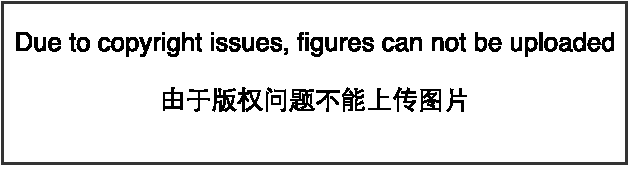
\includegraphics{figure.pdf}}
\else
\centerline{\includegraphics{Chapter3/figures/normal_color}}
\fi
\caption{Tmp}
\label{fig:chap3_normal_color}
\end{figure}

\gls{normal_distribution}被两个参数控制,$\mu \in \SetR$和$\sigma \in (0, \infty)$。
参数$\mu$给出了中心峰值的坐标,这也是分布的均值:$\SetE[\RSx] = \mu$。
分布的\gls{standard_error}用$\sigma$表示,\gls{variance}用$\sigma^2$表示。

当我们要对\gls{PDF}求值时,我们需要对$\sigma$平方并且取倒数。
当我们需要经常对不同参数下的\gls{PDF}求值时,一种更高效的使用参数描述分布的方式是使用参数$\beta \in (0, \infty)$,来控制分布的\firstgls{precision}或者方差的倒数:
\begin{equation}
\CalN(x; \mu, \beta^{-1}) = \sqrt{\frac{\beta}{2\pi}} \exp \left(  -\frac{1}{2}\beta (x-\mu)^2 \right).
\label{eq:3.22}
\end{equation}

采用\gls{normal_distribution}在很多应用中都是一个明智的选择。
当我们缺乏对于某个实数上分布的先验知识而不知道该选择怎样的形式时,\gls{normal_distribution}是默认的比较好的选择,这里有两个原因。

% -- 61 --

第一,我们想要建模的很多分布真实情况是比较接近\gls{normal_distribution}的。
\firstgls{central_limit_theorem}说明很多独立\gls{RV}的和近似服从\gls{normal_distribution}。
这意味着在实际中,很多复杂系统都可以被成功建模成\gls{normal_distribution}的噪声,即使系统可以被分解成具有更多结构化行为的各个部分。

第二,在具有相同方差的所有可能的\gls{PD}中,\gls{normal_distribution}在实数上具有最大的不确定性。
我们因此可以认为\gls{normal_distribution}是对模型加入的先验知识量最少的分布。
充分利用和证明这个想法需要更多的数学工具,我们推迟到\ref{sec:calculus_of_variations}节进行讲解。

\gls{normal_distribution}可以推广到$\SetR^n$空间,这种情况下被称为\firstgls{multivariate_normal_distribution}。
它的参数是一个正定对称矩阵$\bm{\Sigma}$:
\begin{equation}
\CalN(\bm{x}; \bm{\mu}, \bm{\Sigma}) = \sqrt{ \frac{1}{ (2\pi)^n \det(\bm{\Sigma})}}  \exp \left ( -\frac{1}{2} (\bm{x}-\bm{\mu})^\top \bm{\Sigma}^{-1} (\bm{x}- \bm{\mu}) \right).
\end{equation}

参数$\bm{\mu}$仍然表示分布的均值,只不过现在是向量值的。
参数$\bm{\Sigma}$给出了分布的\gls{covariance_matrix}。
和单变量的情况类似,当我们希望对很多不同参数下的\gls{PDF}多次求值时,\gls{covariance_matrix}并不是一个很高效的用参数描述分布的方法,因为对\gls{PDF}求值时需要对$\bm{\Sigma}$求逆。
我们可以用一个\firstgls{precision_matrix}
$\bm{\beta}$ 进行替代:
\begin{equation}
\CalN(\bm{x}; \bm{\mu}, \bm{\beta}^{-1}) = \sqrt{ \frac{\det(\bm{\beta})}{ (2\pi)^n}}  \exp \left ( -\frac{1}{2} (\bm{x}-\bm{\mu})^\top \bm{\beta} (\bm{x}- \bm{\mu}) \right).
\end{equation}

% -- 62 --

我们常常把\gls{covariance_matrix}固定成一个对角阵。
一个更简单的版本是\firstgls{isotropic}\gls{gaussian_distribution},它的\gls{covariance_matrix}是一个标量乘以单位阵。

\subsection{\gls{exponential_distribution}和\gls{laplace_distribution}}
\label{sec:exponential_and_laplace_distributions}

在深度学习中,我们经常会需要一个在$x=0$点处取得边界点(sharp point)的分布。
为了实现这一目的,我们可以使用\firstgls{exponential_distribution}:
\begin{equation}
p(x; \lambda) = \lambda \bm{1}_{x\ge 0} \exp(-\lambda x).
\end{equation}
指数分布使用\gls{indicator_function}(indicator function)$\bm{1}_{x\ge 0}$来使得当$x$取负值时的概率为零。

一个非常相关的\gls{PD}是\firstgls{laplace_distribution},它允许我们在任意一点$\mu$处设置\gls{PD}的峰值
\begin{equation}
\text{Laplace}(x; \mu, \gamma) = \frac{1}{2\gamma} \exp \left( -\frac{|x-\mu|}{\gamma}  \right)
\end{equation}

\subsection{\gls{dirac_distribution}和\gls{empirical_distribution}}
\label{sec:the_dirac_distribution_and_empirical_distribution}

在一些情况下,我们想要所有的概率都集中在一个点上。
这可以通过\firstgls{dirac_delta_function}$\delta(x)$定义\gls{PDF}来实现:
\begin{equation}
p(x) = \delta(x-\mu).
\end{equation}
\gls{dirac_delta_function}被定义成除了0以外的其他点的值都为0,但是积分为1。
\gls{dirac_delta_function}不像普通函数一样对$x$的每一个值都有一个实数值的输出,它是一种不同类型的数学对象,被称为\firstgls{generalized_function},\gls{generalized_function}是依据积分性质定义的数学对象。
我们可以把\gls{dirac_delta_function}想成一系列函数的极限点,这一系列函数把除$\mu$以外的所有点的概率密度越变越小。

% -- 63 --

通过把$p(x)$定义成$\delta$函数左移$-\mu$个单位,我们得到了一个在$x=\mu$ 处具有无限窄也无限高的峰值的\gls{PDF}。

\gls{dirac_distribution}经常作为\firstgls{empirical_distribution}的一个组成部分出现:
\begin{equation}
\hat{p}(\bm{x}) = \frac{1}{m} \sum_{i=1}^m \delta(\bm{x} - \bm{x}^{(i)})
\end{equation}
\gls{empirical_distribution}将概率密度$\frac{1}{m}$赋给$m$个点$\bm{x}^{(1)}, \ldots, \bm{x}^{(m)}$中的每一个,这些点是给定的数据集或者采样的集合。
\gls{dirac_delta_function}只对定义连续型\gls{RV}的\gls{empirical_distribution}是必要的。
对于离散型\gls{RV},情况更加简单:\gls{empirical_distribution}可以被定义成一个\gls{multinoulli_distribution},对于每一个可能的输入,其概率可以简单地设为在训练集上那个输入值的\firstgls{empirical_frequency}。

当我们在训练集上训练模型时,我们可以认为从这个训练集上得到的\gls{empirical_distribution}指明了我们采样来源的分布。
关于\gls{empirical_distribution}另外一种重要的观点是,它是训练数据的似然最大的那个概率密度函数(见\ref{sec:maximum_likelihood_estimation}节)。

\subsection{分布的混合}
\label{sec:mixtures_of_distributions}

通过组合一些简单的\gls{PD}来定义新的\gls{PD}也是很常见的。
一种通用的组合方法是构造\firstgls{mixture_distribution}。
混合分布由一些组件(component)分布构成。
每次实验,样本是由哪个组件分布产生的取决于从一个\gls{multinoulli_distribution}中采样的结果:
\begin{equation}
P(\RSx) = \sum_i P(\RSc = i) P(\RSx | \RSc = i)
\end{equation}
这里$P(\RSc)$是对各组件的一个\gls{multinoulli_distribution}。

我们已经看过一个混合分布的例子了:实值变量的\gls{empirical_distribution}对于每一个训练实例来说,就是以\gls{dirac_distribution}为组件的混合分布。

% -- 64 --

混合模型是组合简单\gls{PD}来生成更丰富的分布的一种简单策略。
在第\ref{chap:structured_probabilistic_models_for_deep_learning}章中,我们探讨从简单\gls{PD}构建复杂模型的更详细的技术。

混合模型使我们能够一瞥以后会用到的一个非常重要的概念——\firstgls{latent_variable}。
\gls{latent_variable}是我们不能直接观测到的\gls{RV}。
混合模型的组件变量$\RSc$就是其中一个例子。
\gls{latent_variable}在联合分布中可能和$\RSx$有关,在这种情况下,$P(\RSx, \RSc) = P(\RSx | \RSc)P(\RSc)$。
\gls{latent_variable}的分布$P(\RSc)$以及关联\gls{latent_variable}和观测变量的条件分布$P(\RSx |\RSc)$,共同决定了分布$P(\RSx)$的形状,尽管描述$P(\RSx)$时可能并不需要\gls{latent_variable}。
\gls{latent_variable}会在\ref{sec:learning_about_dependencies}一节中深入讨论。

一个非常强大且常见的混合模型是\firstgls{GMM},它的组件$p(\RSx | \RSc= i)$是\gls{gaussian_distribution}。
每个组件都有各自的参数,均值$\bm{\mu}^{(i)}$和\gls{covariance_matrix}$\bm{\Sigma}^{(i)}$。
有一些混合可以有更多的限制。
例如,\gls{covariance_matrix}可以通过$\bm{\Sigma}^{(i)} = \bm{\Sigma}, \forall i$的形式在组件之间共享参数。
和单个\gls{gaussian_distribution}一样,\gls{GMM}有时会限制每个组件的\gls{covariance_matrix}是对角的或者各向同性的(标量乘以单位矩阵)。

除了均值和\gls{covariance}以外,\gls{GMM}的参数指明了给每个组件$i$的\firstgls{prior_probability}$\alpha_i = P(\RSc = i)$。
``先验''一词表明了在观测到$\RSx$\emph{之前}传递给模型关于$\RSc$的信念。
作为对比,$P(\RSc | \bm{x})$是\firstgls{posterior_probability},因为它是在观测到$\RSx$\emph{之后}进行计算的。
\gls{GMM}是概率密度的\firstgls{universal_approximator},在这种意义上,任何平滑的概率密度都可以用具有足够多组件的\gls{GMM}以任意精度来逼近。

图\ref{fig:chap3_mog_color}演示了某个\gls{GMM}生成的样例。
\begin{figure}[!htb]
\ifOpenSource
\centerline{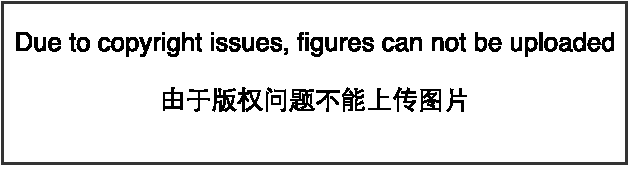
\includegraphics{figure.pdf}}
\else
\centerline{\includegraphics{Chapter3/figures/mog_color}}
\fi
\caption{Tmp}
\label{fig:chap3_mog_color}
\end{figure}


\section{常用函数的一些性质}
\label{sec:useful_properties_of_common_functions}

某些函数在处理\gls{PD}时经常会出现,尤其是深度学习的模型中用到的\gls{PD}。

% -- 65 --

其中一个函数是\textbf{\gls{logistic_sigmoid}}函数:
\begin{equation}
\sigma(x) = \frac{1}{1+\exp(-x)}.
\end{equation}
\gls{logistic_sigmoid}函数通常用来产生\gls{bernoulli_distribution}中的参数$\phi$,因为它的范围是$(0,1)$,处在$\phi$的有效取值范围内。
图\ref{fig:chap3_sigmoid_color}给出了sigmoid函数的图示。
sigmoid函数在变量取绝对值非常大的正值或负值时会出现\firstgls{saturate}现象,意味着函数会变得很平,并且对输入的微小改变会变得不敏感。
\begin{figure}[!htb]
\ifOpenSource
\centerline{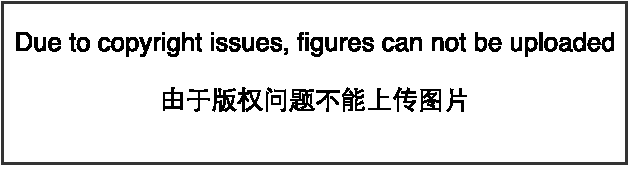
\includegraphics{figure.pdf}}
\else
\centerline{\includegraphics{Chapter3/figures/sigmoid_color}}
\fi
\caption{Tmp}
\label{fig:chap3_sigmoid_color}
\end{figure}

另外一个经常遇到的函数是\firstgls{softplus_function}\citep{secondorder:2001:nips}:
\begin{equation}
\zeta(x) = \log(1+\exp(x))
\end{equation}
\gls{softplus_function}可以用来产生\gls{normal_distribution}的$\beta$和$\sigma$参数,因为它的范围是$(0,\infty)$。
当处理包含sigmoid函数的表达式时它也经常出现。
\gls{softplus_function}名来源于它是另外一个函数的平滑形式,这个函数是
\begin{equation}
x^+ = \max(0, x).
\end{equation}
图\ref{fig:chap3_softplus_color}给出了\gls{softplus_function}的图示。
\begin{figure}[!htb]
\ifOpenSource
\centerline{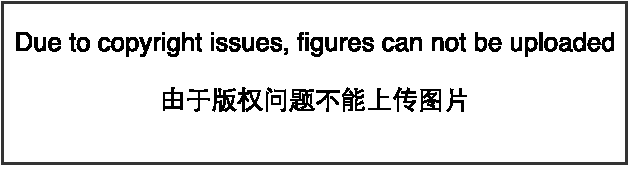
\includegraphics{figure.pdf}}
\else
\centerline{\includegraphics{Chapter3/figures/softplus_color}}
\fi
\caption{Tmp}
\label{fig:chap3_softplus_color}
\end{figure}


% -- 66 --

下面一些性质非常有用,你可能会希望记下来:
\begin{gather}
\sigma(x) = \frac{\exp(x)}{\exp(x)+\exp(0)}\\
\frac{d}{dx} \sigma(x) = \sigma(x)(1 - \sigma(x))\\
1-\sigma(x) = \sigma(-x)\\
\log \sigma(x) = -\zeta(-x)\\
\frac{d}{dx} \zeta(x) = \sigma(x)\\
\forall x \in (0, 1), \sigma^{-1}(x) = \log \left (  \frac{x}{1-x} \right)\\
\forall x>0, \zeta^{-1}(x) = \log(\exp(x) - 1)\\
\zeta(x) = \int_{-\infty}^x \sigma(y) dy\\
\zeta(x) - \zeta(-x) = x
\label{eq: 3.41}
\end{gather}
函数$\sigma^{-1}(x)$在统计学中被称为\firstgls{logit},但这个函数在机器学习中很少用到。

% -- 67 --

公式\ref{eq: 3.41}为函数名``softplus''提供了其他的正当理由。
\gls{softplus_function}被设计成\firstgls{positive_part_function}的平滑版本,这个\gls{positive_part_function}是指$x^+ = \max \{ 0, x\}$。
与\gls{positive_part_function}相对的是\firstgls{negative part function}$x^- = \max\{ 0, -x\}$。
为了获得类似\gls{negative part function}的一个平滑函数,我们可以使用$\zeta(-x)$。
就像$x$可以用它的正部和负部通过等式$x^+ - x^- = x$恢复一样,我们也可以用同样的方式对$\zeta(x)$和$\zeta(-x)$进行操作,就像公式\ref{eq: 3.41}中那样。

\section{\gls{bayes_rule}}
\label{sec:bayes_rule}

我们经常会需要在已知$P(\RSy | \RSx)$时计算$P(\RSx | \RSy)$。
幸运的是,如果还知道$P(\RSx)$,我们可以用\firstgls{bayes_rule}来实现这一目的:
\begin{equation}
P(\RSx | \RSy) = \frac{P(\RSx) P(\RSy | \RSx)}{P(\RSy)}.
\end{equation}
注意到$P(\RSy)$出现在上面的公式中,它通常使用$P(\RSy) = \sum_x P(\RSy | x) P(x)$来计算,所以我们并不需要事先知道$P(\RSy)$的信息。

\gls{bayes_rule}可以从\gls{conditional_probability}的定义直接推导得出,但我们最好记住这个公式的名字,因为很多文献通过名字来引用这个公式。
这个公式是以Reverend Thomas Bayes来命名的,他是第一个发现这个公式的特例的人。
这里介绍的一般形式由Pierre-Simon Laplace独立发现。

\section{连续型变量的技术细节}
\label{sec:technical_details_of_continuous_variables}

连续型\gls{RV}和\gls{PDF}的深入理解需要用到数学分支\firstgls{measure_theory}的相关内容来扩展概率论。
\gls{measure_theory}超出了本书的范畴,但我们可以简要勾勒一些\gls{measure_theory}用来解决的问题。

在\ref{sec:continuous_variables_and_probability_density_functions}节中,我们已经看到连续型向量值\gls{RV}$\RVx$落在某个集合$\SetS$ 中的概率是通过$p(\bm{x})$对集合$\SetS$积分得到的。
对于集合$\SetS$的一些选择可能会引起悖论。
例如,构造两个集合$\SetS_1$和$\SetS_2$使得$p(\bm{x}\in \SetS_1) + p(\bm{x}\in \SetS_2)>1$并且$\SetS_1 \cap \SetS_2 = \emptyset$是可能的。
这些集合通常是大量使用了实数的无限精度来构造的,例如通过构造分形形状(fractal-shaped)的集合或者是通过有理数相关集合的平移来定义的集合。
\footnote{Banach-Tarski定理给出了这类集合的一个有趣的例子。}
\gls{measure_theory}的一个重要贡献就是提供了一些集合的特征使得我们我们在计算概率时不会遇到悖论。
在本书中,我们只对描述相对简单的集合进行积分,所以\gls{measure_theory}的这个方面不会成为一个相关考虑。

% -- 68 --

对于我们的目的,\gls{measure_theory}更多的是用来描述那些适用于$\SetR^n$上的大多数点的定理的,而不是只适用于一些小的情况。
\gls{measure_theory}提供了一种严格的方式来描述那些非常微小的点集。
这种集合被称为``\firstgls{measure_zero}''的。
我们不会在本书中给出这个概念的正式定义。
然而,直观地理解这个概念是有用的,我们可以认为零测度集在我们的度量空间中不占有任何的体积。
例如,在$\SetR^2$空间中,一条直线的测度为零,而填充的多边形具有正的测度。
类似的,一个单独的点的测度为零。
可数多个零测度集的并仍然是零测度的(所以所有有理数构成的集合测度为零)。

另外一个有用的\gls{measure_theory}中的术语是``\firstgls{almost_everywhere}''。
某个性质如果是几乎处处都成立的,那么它在整个空间中除了测度为零的集合以外都是成立的。
因为这些例外只在空间中占有极其微小的量,它们在多数应用中都可以被放心地忽略。
概率论中的一些重要结果对于离散值成立但对于连续值只能是``几乎处处''成立。

连续型\gls{RV}的另一技术细节,涉及到处理那种相互之间是彼此的确定性函数的连续型变量。
假设我们有两个\gls{RV}$\RVx$和$\RVy$满足$\bm{y} = g(\bm{x})$,其中$g$是可逆的、连续可微的函数。
可能有人会想$p_y(\bm{y}) = p_x(g^{-1}(\bm{y}))$。
但实际上这并不对。

举一个简单的例子,假设我们有两个标量值\gls{RV}$\RSx$和$\RSy$,并且满足$\RSy= \frac{\RSx}{2}$以及$\RSx \sim U(0, 1)$。
如果我们使用$p_y(y) = p_x(2y)$,那么$p_y$ 除了区间$[0, \frac{1}{2}]$以外都为0,并且在这个区间上的值为1。
这意味着
\begin{equation}
\int p_y(y)dy = \frac{1}{2},
\end{equation}
而这违背了概率密度的定义(积分为1)。

这个常见错误之所以错是因为它没有考虑到引入函数$g$后造成的空间变形。
回忆一下,$\bm{x}$落在无穷小的体积为$\delta \bm{x}$的区域内的概率为$p(\bm{x})\delta\bm{x}$。
因为$g$可能会扩展或者压缩空间,在$\bm{x}$空间内的包围着$\bm{x}$ 的无穷小体积在$\bm{y}$空间中可能有不同的体积。

% -- 69 --

为了看出如果改正这个问题,我们回到标量值的情况。
我们需要保持下面这个性质:
\begin{equation}
|p_y(g(x))dy| = |p_x(x)dx|.
\end{equation}
求解上式,我们得到
\begin{equation}
p_y(y) = p_x(g^{-1}(y)) \left \vert \frac{\partial x}{\partial y} \right \vert
\end{equation}
或者等价地,
\begin{equation}
p_x(x) = p_y(g(x)) \left | \frac{\partial g(x)}{\partial x} \right |.
\end{equation}

在高维空间中,微分运算扩展为\firstgls{jacobian_matrix}的行列式——矩阵的每个元素为$J_{i, j} = \frac{\partial x_i}{\partial y_j}$。
因此,对于实数值的向量$\bm{x}$和$\bm{y}$,
\begin{equation}
p_x(\bm{x}) = p_y(g(\bm{x})) \left | \det \left ( \frac{\partial g(\bm{x})}{\partial \bm{x}} \right) \right |.
\end{equation}

\section{信息论}
\label{sec:information_theory}

信息论是应用数学的一个分支,主要研究的是对一个信号能够提供信息的多少进行量化。
它最初被发明是用来研究在一个含有噪声的信道上用离散的字母表来发送消息,例如通过无线电传输来通信。
在这种情况下,信息论告诉我们如何设计最优编码,以及计算从一个特定的\gls{PD}上采样得到、使用多种不同的编码机制的消息的期望长度。
在机器学习中,我们也可以把信息论应用在连续型变量上,而信息论中一些消息长度的解释不怎么使用。
信息论是电子工程和计算机科学的许多领域的基础。
在本书中,我们主要使用信息论的一些关键思想来描述\gls{PD}或者量化\gls{PD}之间的相似性。
有关信息论的更多细节,参见\cite{cover-book2006}或者\cite{MacKay03}。

信息论的基本想法是一个不太可能的事件居然发生了,要比一个非常可能的事件发生,能提供更多的信息。
消息说:``今天早上太阳升起''信息量是如此之少以至于没有必要发送,但一条消息说:``今天早上有日食''信息量就很丰富。

% -- 70 --

我们想要通过这种基本想法来量化信息。
特别地,
\begin{itemize}
\item 非常可能发生的事件信息量要比较少,并且极端情况下,确保能够发生的事件应该没有信息量。

\item 更不可能发生的事件要具有更高的信息量。

\item 独立事件应具有增量的信息。
例如,投掷的硬币两次正面朝上传递的信息量,应该是投掷一次硬币正面朝上的信息量的两倍。
\end{itemize}

为了满足上述三个性质,我们定义一个事件$\RSx = x$的\firstgls{self_information}为
\begin{equation}
I(x) = -\log P(x)
\end{equation}
在本书中,我们总是用$\log$来表示自然对数,底数为$e$。
因此我们定义的$I(x)$单位是\firstgls{nats}。
一奈特是以$\frac{1}{e}$的概率观测到一个事件时获得的信息量。
其他的材料中使用底数为2的对数,单位是\firstgls{bits}或者\firstgls{shannons};通过比特度量的信息只是通过奈特度量信息的常数倍。

当$\RSx$是连续的,我们使用类似的关于信息的定义,但有些来源于离散形式的性质就丢失了。
例如,一个具有单位密度的事件信息量仍然为0,但是不能保证它一定发生。

\gls{self_information}只处理单个的输出。
我们可以用\firstgls{Shannon_entropy}来对整个\gls{PD}中的不确定性总量进行量化:
\begin{equation}
H(\RSx) = \SetE_{\RSx \sim P}[I(x)] = -\SetE_{\RSx \sim P}[\log P(x)].
\end{equation}
也记作$H(P)$。
换言之,一个分布的\gls{Shannon_entropy}是指遵循这个分布的事件所产生的期望信息总量。
它给出了对,依据\gls{PD}$P$生成的符号,进行编码所需的比特数的平均意义上的下界(如果对数的底是2的话,否则单位有所不同)。
那些接近确定性的分布(输出几乎可以确定)具有较低的熵;那些接近\gls{uniform_distribution}的\gls{PD}具有较高的熵。
图\ref{fig:chap3_entropy_demo_color}给出了一个说明。
当$\RSx$是连续的,\gls{Shannon_entropy}被称为\firstgls{differential_entropy}。
\begin{figure}[!htb]
\ifOpenSource
\centerline{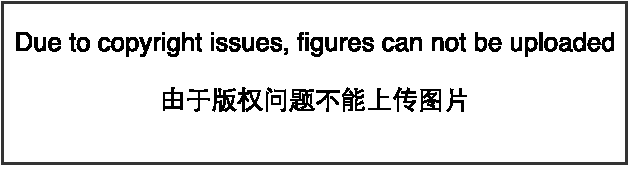
\includegraphics{figure.pdf}}
\else
\centerline{\includegraphics{Chapter3/figures/entropy_demo_color}}
\fi
\caption{Tmp}
\label{fig:chap3_entropy_demo_color}
\end{figure}


% -- 71 --

如果我们对于同一个\gls{RV}$\RSx$有两个单独的\gls{PD}$P(\RSx)$和$Q(\RSx)$,我们可以使用\firstgls{KL_divergence}来衡量这两个分布的差异:
\begin{equation}
D_{\text{KL}}(P||Q) = \SetE_{\RSx \sim P} \left [  \log \frac{P(x)}{Q(x)} \right ] = \SetE_{\RSx \sim P} [\log P(x) - \log Q(x)].
\end{equation}

在离散型变量的情况下,\gls{KL_divergence}衡量的是,当我们使用一种被设计成能够使得\gls{PD}$Q$ 产生的消息的长度最小的编码时,发送包含由\gls{PD}$P$产生的符号的消息时,所需要的额外信息量(如果我们使用底数为2的对数时信息量用比特衡量,但在机器学习中,我们通常用奈特和自然对数。)

\gls{KL_divergence}有很多有用的性质,最重要的是它是非负的。
\gls{KL_divergence}为0当且仅当$P$和$Q$在离散型变量的情况下是相同的分布,或者在连续型变量的情况下是``几乎处处''相同的。
因为\gls{KL_divergence}是非负的并且衡量的是两个分布之间的差异,它经常被用作分布之间的某种距离。
然而,它并不是真的距离因为它不是对称的:对于某些$P$和$Q$,$D_\text{KL}(P||Q) \ne D_\text{KL}(Q||P)$。
这种非对称性意味着选择$D_\text{KL}(P||Q)$还是$D_\text{KL}(Q||P)$影响很大。
更多细节可以看图\ref{fig:chap3_kl_direction_color}。
\begin{figure}[!htb]
\ifOpenSource
\centerline{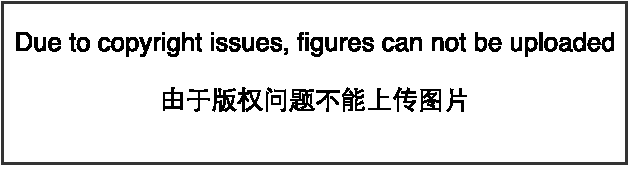
\includegraphics{figure.pdf}}
\else
\centerline{\includegraphics{Chapter3/figures/kl_direction_color}}
\fi
\caption{Tmp}
\label{fig:chap3_kl_direction_color}
\end{figure}


% -- 72 --

一个和\gls{KL_divergence}密切联系的量是\firstgls{cross_entropy}$H(P, Q) = H(P) + D_\text{KL}(P||Q)$,它和\gls{KL_divergence}很像但是缺少左边一项:
\begin{equation}
H(P, Q) = -\SetE_{\RSx\sim P} \log Q(x).
\end{equation}
针对$Q$最小化互信息等价于最小化\gls{KL_divergence},因为$Q$并不参与被省略的那一项。

当计算这些量时,经常会遇到$0\log 0$这个表达式。
按照惯例,在信息论中,我们对于这个表达式这样处理$\lim_{x \to 0} x\log x = 0$。

% -- 73 --

\section{\gls{structured_probabilistic_models}}
\label{sec:structured_probabilistic_models}

机器学习的算法经常会涉及到在非常多的\gls{RV}上的\gls{PD}。
通常,这些\gls{PD}涉及到的直接相互作用都是介于非常少的变量之间的。
使用单个函数来描述整个\gls{joint_probability_distribution}是非常低效的(无论是计算还是统计)。

代替使用单一的函数来表示\gls{PD},我们可以把\gls{PD}分割成许多因子的乘积形式。
例如,假设我们有三个\gls{RV}$\RSa, \RSb$和$\RSc$,并且$\RSa$影响$\RSb$的取值,$\RSb$影响$\RSc$的取值,但是$\RSa$和$\RSc$在给定$\RSb$时是条件独立的。
我们可以把全部三个变量的\gls{PD}重新表示为两个变量的\gls{PD}的连乘形式:
\begin{equation}
p(\RSa, \RSb, \RSc) = p(\RSa)p(\RSb| \RSa)p(\RSc|\RSb).
\end{equation}

这种因子分解可以极大地减少用来描述一个分布的参数的数量。
每个因子使用的参数数目是它的变量数目的指数倍。
这意味着,如果我们能够找到一种使每个因子分布具有更少变量的因子分解方法,我们就能极大地降低表示联合分布的成本。

我们可以用图来描述这种因子分解。
这里我们使用的是图论中的``图''的概念:由一些可以通过边互相连接的顶点的集合构成。
当我们用图来表示这种\gls{PD}的因子分解,我们把它称为\firstgls{structured_probabilistic_model}或者\firstgls{graphical_model}。

有两种主要的\gls{structured_probabilistic_models}:有向的和无向的。
两种图模型使用图$\CalG$,其中图的每个节点对应着一个\gls{RV},连接两个\gls{RV}的边意味着\gls{PD}可以表示成这两个\gls{RV}之间的直接作用。

\firstgls{directed}模型使用带有有向边的图,它们用\gls{conditional_probability}分布来表示因子分解,就像上面的例子。
特别地,有向模型对于分布中的每一个\gls{RV}$\RSx_i$都包含着一个影响因子,这个组成$\RSx_i$\gls{conditional_probability}的影响因子被称为$\RSx_i$的双亲,记为$Pa_\CalG(\RSx_i)$:
\begin{equation}
p(\RVx) = \prod_i p(\RSx_i | Pa_\CalG(\RSx_i)).
\end{equation}
图\ref{fig:chap3_directed}给出了一个有向图的例子以及它表示的\gls{PD}的因子分解。
\begin{figure}[!htb]
\ifOpenSource
\centerline{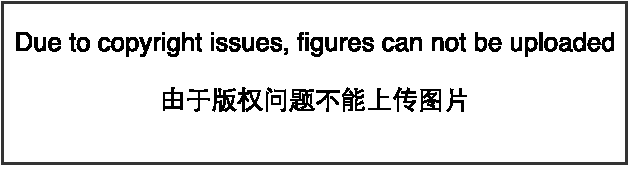
\includegraphics{figure.pdf}}
\else
\centerline{\includegraphics{Chapter3/figures/directed}}
\fi
\caption{Tmp}
\label{fig:chap3_directed}
\end{figure}


% -- 74 --

\firstgls{undirected}模型使用带有无向边的图,它们将因子分解表示成一堆函数;不像有向模型那样,这些函数通常不是任何类型的\gls{PD}。
$\CalG$中任何全部相连的节点构成的集合被称为团。
无向模型中的每个团$\CalC^{(i)}$都伴随着一个因子$\phi^{(i)}(\CalC^{(i)})$。
 这些因子仅仅是函数,并不是\gls{PD}。
 每个因子的输出都必须是非负的,但是并没有像\gls{PD}中那样要求因子的和或者积分为1。

\gls{RV}的联合概率和所有这些因子的乘积\firstgls{proportional}——意味着因子的值越大则可能性越大。
当然,不能保证这种乘积的求和为1。
所以我们需要除以一个归一化常数$Z$来得到归一化的\gls{PD},归一化常数$Z$被定义为$\phi$函数乘积的所有状态的求和或积分。
\gls{PD}为:
\begin{equation}
p(\RVx) = \frac{1}{Z} \prod_i \phi^{(i)} \left (\CalC^{(i)} \right).
\end{equation}
图\ref{fig:chap3_undirected}给出了一个无向图的例子以及它表示的\gls{PD}的因子分解。
\begin{figure}[!htb]
\ifOpenSource
\centerline{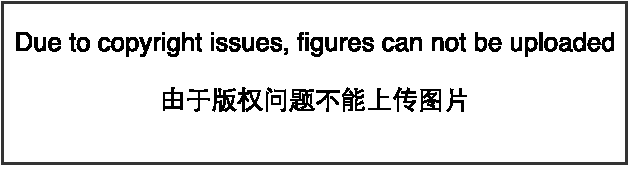
\includegraphics{figure.pdf}}
\else
\centerline{\includegraphics{Chapter3/figures/undirected}}
\fi
\caption{Tmp}
\label{fig:chap3_undirected}
\end{figure}


% -- 75 --

请记住,这些图模型表示的因子分解仅仅是描述\gls{PD}的一种语言。
它们不是互相排斥的\gls{PD}族。
有向或者无向不是\gls{PD}的特性;它是\gls{PD}的一种特殊\firstgls{description}所具有的特性,但是任何的\gls{PD}都可以用两种方式进行描述。

在本书第|||c|||部分和第|||c|||部分中, 我们使用\gls{structured_probabilistic_models}仅仅是作为一门语言,来描述不同的机器学习算法选择表示的直接的概率关系。
一直到研究课题的讨论之前,不会需要用到\gls{structured_probabilistic_models}的深入理解。
在第|||c|||部分的研究课题中,我们会更为详尽地探讨\gls{structured_probabilistic_models}。

本章复习了概率论中与深度学习最为相关的一些基本概念。
还剩下一些基本的数学工具需要讨论:数值方法。

% -- 76 --

% Translator: Shenjian Zhao
\chapter{数值计算}
\label{chap:numerical_computation}

\gls{ML}算法通常需要大量的数值计算。
<BAD>数值计算通常指的是通过迭代地更新解来解决数学问题的算法,而不是解析地提供正确解的符号表达。
常见的操作包括优化(找到最小化或最大化函数值的参数)和线性方程的求解。
对数字计算机来说,即使计算只涉及实数的函数也是困难的,因为实数无法在有限内存下精确表示。

\section{\gls{overflow}和\gls{underflow}}
\label{sec:overflow_and_underflow}
在数字计算机上实现连续数学的基本困难是,我们需要通过有限数量的位模式来表示无限多的实数。
这意味着我们在计算机中表示实数时,几乎都会引入一些近似误差。
在许多情况下,这仅仅是舍入误差。
如果在理论上可行的算法没有被设计为最小化舍入误差的累积,可能会在实践中失效,因此舍入误差是有问题的(特别是许多操作复合时)。

一种特别的毁灭性舍入误差是\firstgls{underflow}。
当接近零的数被四舍五入为零时发生\gls{underflow}。
许多函数会在其参数为零而不是一个很小的正数时才会表现出质的不同。
例如,我们通常要避免被零除(一些软件环境将在这种情况抛出异常,有些会返回一个非数字(not-a-number)的占位符)或取零的对数(这通常被视为$-\infty$,进一步的算术运算会使其变成非数字)。

% -- 77 --

另一个极具破坏力的数值错误形式是\firstgls{overflow}。
当大量级的数被近似为$\infty$或$-\infty$时发生\gls{overflow}。
进一步的运算通常将这些无限值变为非数字。

必须对\gls{overflow}和\gls{underflow}进行数值稳定的一个例子是\firstgls{softmax}。
\gls{softmax}经常用于预测与\gls{multinoulli}相关联的概率,定义为
\begin{align}
 \text{softmax}(\Vx)_i = \frac{\exp(\Sx_i)}{\sum_{j=1}^n \exp(\Sx_j)}
\end{align}
考虑一下当所有$\Sx_i$都等于某个常数$\Sc$时会发生什么。
从理论分析上说,我们可以发现所有的输出都应该为$\frac{1}{n}$。
从数值计算上说,当$\Sc$量级很大时,这可能不会发生。
如果$\Sc$是很小的负数,$\exp(c)$就会\gls{underflow}。
这意味着\gls{softmax}的分母会变成0,所以最后的结果是未定义的。
当$\Sc$是非常大的正数时,$\exp(c)$的\gls{overflow}再次导致整个表达式未定义。
这两个困难能通过计算$\text{softmax}(\Vz)$同时解决,其中$\Vz = \Vx - \max_i \Sx_i$。
简单的代数计算表明,$\text{softmax}$解析上的函数值不会因为从输入向量减去或加上标量而改变。
减去$\max_i x_i$导致$\exp$的最大参数为$0$,这排除了\gls{overflow}的可能性。
同样地,分母中至少有一个值为1的项,这就排除了因分母\gls{underflow}而导致被零除的可能性。

还有一个小问题。
分子中的\gls{underflow}仍可以导致整体表达式被计算为零。
这意味着,如果我们在计算$\log ~\text{softmax}(\Vx)$时先计算$\text{softmax}$再把结果传给$\log$函数,会错误地得到$-\infty$。
相反,我们必须实现一个单独的函数,并以数值稳定的方式计算$\log \text{softmax}$。
可以使用相同的技巧稳定$\log \text{softmax}$函数。

在大多数情况下,我们没有明确地对实现本书描述的各种算法时所涉及的数值考虑进行详细说明。
底层库的开发者在实现\gls{DL}算法时应该牢记数值问题。
本书的大多数读者可以简单地依赖保证数值稳定的底层库。
在某些情况下,有可能在实现一个新的算法时自动保持数值稳定。
Theano\citep{bergstra+al:2010-scipy,Bastien-2012}就是这样软件包的一个例子,它能自动检测并稳定\gls{DL}中许多常见的数值不稳定的表达式。

% -- 78 --

\section{\gls{poor_conditioning}}
\label{sec:poor_conditioning}

条件数表明函数相对于输入的微小变化而变化的快慢程度。
输入被轻微扰动而迅速改变的函数对于科学计算来说是可能是有问题的,因为输入中的舍入误差可能导致输出的巨大变化。

考虑函数$f(\Vx) = \MA^{-1} \Vx$。
当$\MA \in \SetR^{n \times n}$ 具有特征值分解时,其条件数为
\begin{align}
 \underset{i,j}{\max} \Bigg| \frac{\lambda_i}{ \lambda_j} \Bigg|.
\end{align}
这是最大和最小特征值的模之比。
当该数很大时,矩阵求逆对输入的误差特别敏感。

这种敏感性是矩阵本身的固有特性,而不是矩阵求逆期间舍入误差的结果。
即使我们乘以完全正确的矩阵逆,\gls{poor_conditioning}的矩阵也会放大预先存在的误差。
在实践中,该错误将与求逆过程本身的数值误差进一步复合。



\section{基于梯度的优化方法}
\label{sec:gradient_based_optimization}

大多数\gls{DL}算法涉及某种形式的优化。
优化指的是改变$\Vx$以最小化或最大化的某个函数$f(\Vx)$的任务。
我们通常以最小化$f(\Vx)$指代大多数最优化问题。
最大化可经由最小化算法最小化$-f(\Vx)$来实现。

我们希望最小化或最大化的函数叫做\firstgls{objective_function}或\firstgls{criterion}。
当我们对其进行最小化时,我们也把它叫做\firstgls{cost_function},\firstgls{loss_function}或\firstgls{error_function}。
虽然有些机器学习著作赋予这些名称特殊的意义,但在这本书中我们交替使用这些术语。

我们经常使用一个上标$*$表示最小化或最大化函数的$\Vx$值。
如我们记$\Vx^*=\argmin f(\Vx)$。

我们假设读者已经熟悉微积分,这里简要回顾微积分概念如何与优化联系。

% -- 79 --

假设我们有一个函数$\Sy = f(\Sx)$, 其中$\Sx$和$\Sy$是实数。
这个函数的\firstgls{derivative}记为$f^\prime(x)$或$\frac{dy}{dx}$。
导数$f^\prime(\Sx)$代表$f(\Sx)$在点$x$处的斜率。
<BAD>换句话说,它表明需要如何缩放输入的小变化以在输出获得相应的变化:
$f(\Sx+\epsilon) \approx f(\Sx) + \epsilon f^\prime(\Sx) $。

因此\gls{derivative}对于最小化一个函数很有用,因为它告诉我们如何更改$x$来略微地改善$y$。
例如,我们知道对于足够小的$\epsilon$来说, $f(\Sx-\epsilon \text{sign}(f^\prime(\Sx)) )$是比$f(\Sx)$小的。
因此我们可以将$\Sx$往\gls{derivative}的反方向移动一小步来减小$f(\Sx)$。
这个技术被称为\firstgls{GD}\citep{cauchy1847}。
图\ref{fig:chap4_gradient_descent_color}展示了一个例子。
\begin{figure}[!htb]
\ifOpenSource
\centerline{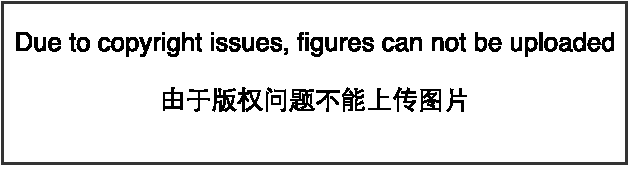
\includegraphics{figure.pdf}}
\else
\centerline{\includegraphics{Chapter4/figures/gradient_descent_color}}
\fi
\caption{TODO}
\label{fig:chap4_gradient_descent_color}
\end{figure}

% -- 80 --

当$f^\prime(\Sx)=0$,\gls{derivative}无法提供往哪个方向移动的信息。
$ f^\prime(\Sx)=0 $的点称为\firstgls{critical_points}或\firstgls{stationary_point}。
一个\firstgls{local_minimum}意味着这个点的$f(\Sx)$小于所有邻近点,因此不可能通过移动无穷小的步长来减小$f(\Sx)$。
一个\firstgls{local_maximum}是$f(x)$意味着这个点的$f(\Sx)$大于所有邻近点,因此不可能通过移动无穷小的步长来增大$f(x)$。
有些\gls{critical_points}既不是最小点也不是最大点。这些点被称为\firstgls{saddle_points}。
见图\ref{fig:chap4_critical_color}给出的各种临界点的例子。
\begin{figure}[!htb]
\ifOpenSource
\centerline{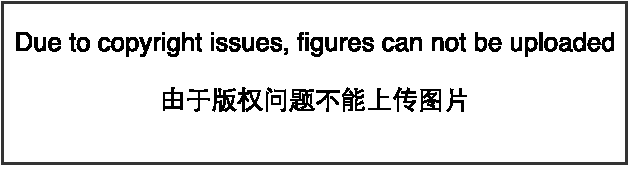
\includegraphics{figure.pdf}}
\else
\centerline{\includegraphics{Chapter4/figures/critical_color}}
\fi
\caption{TODO}
\label{fig:chap4_critical_color}
\end{figure}

使$f(x)$取得全局最小值的点是\firstgls{global_minimum}。
只有一个\gls{global_minimum}或存在多个\gls{global_minimum}的函数是有可能的。
还可能存在不是全局最优的\gls{local_minimum}。
在\gls{DL}的背景下,我们优化的函数可能含有许多不是最优的\gls{local_minimum},或许多被非常平坦的区域包围的\gls{saddle_points}。
尤其是当输入是多维的时候,所有这些都将使优化变得困难。
因此,我们通常寻找$f$非常小的值,但在任何形式意义下并不一定是最小。
见图\ref{fig:chap4_approx_opt_color}的例子。
\begin{figure}[!htb]
\ifOpenSource
\centerline{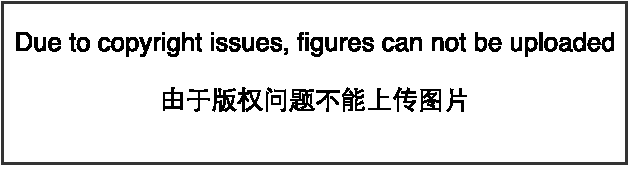
\includegraphics{figure.pdf}}
\else
\centerline{\includegraphics{Chapter4/figures/approx_opt_color}}
\fi
\caption{TODO}
\label{fig:chap4_approx_opt_color}
\end{figure}

我们经常最小化具有多维输入的函数:$f: \SetR^n \rightarrow \SetR $。 
为了使``最小化''的概念有意义,输出必须是一维的(标量)。

% -- 81 --

我们必须利用\firstgls{partial_derivatives}的概念针对具有多维输入的函数。
\gls{partial_derivatives}$\frac{\partial}{\partial \Sx_i}f(\Vx)$衡量点$\Vx$处只有$x_i$增加时$f(\Vx)$如何变化。
\firstgls{gradient}是相对一个向量求导的\gls{derivative}:$f$的导数是包含所有\gls{partial_derivatives}的向量,记为$\nabla_{\Vx} f(\Vx)$。
\gls{gradient}的第$i$的元素是$f$关于$x_i$的\gls{partial_derivatives}。
在多维情况下,\gls{critical_points}是\gls{gradient}中所有元素都为零的点。

在$\Vu$(单位向量)方向的\firstgls{directional_derivative}是函数$f$在$\Vu$方向的斜率。
换句话说,\gls{directional_derivative}是函数$f(\Vx + \alpha \Vu)$关于$\alpha$的\gls{derivative}(在$\alpha = 0$时取得)。
使用链式法则,我们可以看到当$\alpha=0$时,$\frac{\partial}{\partial \alpha} f(\Vx + \alpha \Vu) = \Vu^\Tsp \nabla_{\Vx} f(\Vx)$。

为了最小化$f$,我们希望找到使$f$下降得最快的方向。
计算\gls{directional_derivative}:
\begin{align}
 \underset{\Vu, \Vu^\Tsp\Vu = 1}{\min} \Vu^\Tsp & \nabla_{\Vx} f(\Vx) \\
 = \underset{\Vu, \Vu^\Tsp\Vu = 1}{\min} \| \Vu \|_2 \| &\nabla_{\Vx}f(\Vx) \|_2 \cos \theta
\end{align}
其中$\theta$是$\Vu$与\gls{gradient}的夹角。
将$ \| \Vu \|_2 = 1$代入,并忽略与$\Vu$无关的项,就能简化得到$ \underset{\Vu}{\min} \cos \theta $。 
这在$\Vu$与\gls{gradient}方向相反时取得最小。
换句话说,\gls{gradient}向量指向上坡,负\gls{gradient}向量指向下坡。
我们在负\gls{gradient}方向上移动可以减小$f$。
这被称为\textbf{最速下降法}(method of steepest descent)或\firstgls{GD}。

最速下降建议新的点为
\begin{align}
  \Vx' = \Vx - \epsilon \nabla_{\Vx} f(\Vx)
\end{align}
其中$\epsilon$为学习速率,是一个确定步长大小的正标量。
我们可以通过几种不同的方式选择$\epsilon$。
普遍的方式是选择一个小常数。
有时我们通过计算,选择使\gls{directional_derivative}消失的步长。
还有一种方法是根据几个$\epsilon$计算$f(\Vx - \epsilon \nabla_{\Vx} f(\Vx))$, 并选择其中能产生最小\gls{objective_function}值的$\epsilon$。
这种策略被称为\gls{line_search}。

最速下降在\gls{gradient}的每一个元素为零时收敛(或在实践中,很接近零)。
在某些情况下,我们也许能够避免运行该迭代算法,并通过解方程$\nabla_{\Vx} f(\Vx)= 0$直接跳到\gls{critical_points}。

% -- 82 --

虽然\gls{GD}被限制在连续空间中的优化问题,但不断向更好的情况移动一小步(即近似最佳的小移动)的一般概念可以被推广到离散空间。
递增带有离散参数的\gls{objective_function}被称为\firstgls{hill_climbing}算法\citep{Russel+Norvig-book2003}。

\subsection{\gls{gradient}之上:\gls{jacobian}和\gls{hessian}矩阵}
\label{sec:beyond_the_gradient_jacobian_and_hessian_matrices}
有时我们需要计算输入和输出都为向量的函数的所有\gls{partial_derivatives}。
包含所有这样的偏导数的矩阵被称为\firstgls{jacobian}矩阵。
具体来说,如果我们有一个函数:$\Vf: \SetR^m \rightarrow \SetR^n$,$\Vf$的\gls{jacobian}矩阵$\MJ \in \SetR^{n \times m}$定义为$J_{i,j} = \frac{\partial}{\partial \Sx_j} f(\Vx)_i$。

有时,我们也对\gls{derivative}的\gls{derivative}感兴趣,即\firstgls{second_derivative}。
例如,有一个函数$f: \SetR^m \rightarrow \SetR$,$f$的一阶\gls{derivative}(关于$\Sx_j$)关于$x_i$的\gls{derivative}记为$\frac{\partial^2}{\partial \Sx_i \partial \Sx_j} f$。
在一维情况下,我们可以将$\frac{\partial^2}{\partial \Sx^2} f$为$f''(\Sx)$。
\gls{second_derivative}告诉我们的一阶\gls{derivative}将如何随着输入的变化而改变。
它表示只基于\gls{gradient}信息的\gls{GD}步骤是否会产生如我们预期的那样大的改善,因此是重要的。
我们可以认为,\gls{second_derivative}是对\gls{curvature}的衡量。
假设我们有一个二次函数(虽然很多实践中的函数都不是二次,但至少在局部可以很好地用二次近似)。
如果这样的函数具有零\gls{second_derivative},那就没有\gls{curvature}。
也就是一条完全平坦的线,仅用\gls{gradient}就可以预测它的值。
我们使用沿负\gls{gradient}方向大小为$\epsilon$的下降步,当该\gls{gradient}是$1$时,\gls{cost_function}将下降$\epsilon$。
如果\gls{second_derivative}是负的,函数曲线向下凹陷(向上凸出),因此\gls{cost_function}将下降的比$\epsilon$多。
如果\gls{second_derivative}是正的,函数曲线是向上凹陷(向下凸出),
因此\gls{cost_function}将下降的比$\epsilon$少。
从图\ref{fig:chap4_curvature_color}可以看出不同形式的\gls{curvature}如何影响基于\gls{gradient}的预测值与真实的\gls{cost_function}值的关系。
\begin{figure}[!htb]
\ifOpenSource
\centerline{\includegraphics{figure.pdf}}
\else
\centerline{\includegraphics{Chapter4/figures/curvature_color}}
\fi
\caption{TODO}
\label{fig:chap4_curvature_color}
\end{figure}

当我们的函数具有多维输入时,\gls{second_derivative}也有很多。
可以这些导数合并成一个矩阵,称为\firstgls{hessian}矩阵。
\gls{hessian}矩阵$\MH(f)(\Vx)$定义为
\begin{align}
 \MH(f)(\Vx)_{i,j} = \frac{\partial^2}{\partial \Sx_i \partial  \Sx_j} f(\Vx).
\end{align}
\gls{hessian}等价于\gls{gradient}的\gls{jacobian}矩阵。

% -- 83 --

微分算子在任何二阶偏导连续的点处可交换,也就是它们的顺序可以互换:
\begin{align}
 \frac{\partial^2}{\partial \Sx_i \partial \Sx_j} f(\Vx) = \frac{\partial^2}{\partial \Sx_j\partial \Sx_i} f(\Vx) .
\end{align}
这意味着$H_{i,j} = H_{j,i}$, 因此\gls{hessian}矩阵在这些点上是对称的。
在\gls{DL}背景下,我们遇到的大多数函数的\gls{hessian}几乎处处都是对称的。
因为\gls{hessian}矩阵是实对称的,我们可以将其分解成一组实特征值和特征向量的正交。
在特定方向$\Vd$上的\gls{second_derivative}可以写成$\Vd^\Tsp \MH \Vd$。
当$\Vd$是$\MH$的一个特征向量时,这个方向的\gls{second_derivative}就是对应的特征值。
对于其他的方向$\Vd$,方向\gls{second_derivative}是所有特征值的加权平均,权重在0和1之间,且与$\Vd$夹角越小的特征向量有更大的权重。
最大特征值确定最大\gls{second_derivative},最小特征值确定最小\gls{second_derivative}。

% -- 84 --

我们可以通过(方向)\gls{second_derivative}预期一个\gls{GD}步骤能表现得多好。
我们在当前点$\Vx^{(0)}$处作函数$f(\Vx)$的近似二阶\gls{taylor}级数:
\begin{align}
 f(\Vx) \approx f(\Vx^{(0)}) + (\Vx - \Vx^{(0)})^\Tsp \Vg + 
 \frac{1}{2}  (\Vx - \Vx^{(0)})^\Tsp \MH  (\Vx - \Vx^{(0)}),
\end{align}
其中$\Vg$是梯度,$\MH$是$ \Vx^{(0)}$点的\gls{hessian}。
如果我们使用学习速率$\epsilon$,那么新的点$\Vx$将会是$\Vx^{(0)}-\epsilon \Vg$。
代入上述的近似,可得
\begin{align}
 f(\Vx^{(0)} - \epsilon \Vg ) \approx f(\Vx^{(0)})  - \epsilon \Vg^\Tsp \Vg + \frac{1}{2} \epsilon^2 \Vg^\Tsp \MH  \Vg.
\end{align}
其中有3项:函数的原始值、函数斜率导致的预期改善、函数\gls{curvature}导致的校正。
当这最后一项太大时,\gls{GD}实际上是可能向上移动的。
当$\Vg^\Tsp \MH  \Vg$为零或负时,近似的\gls{taylor}级数表明增加$\epsilon$将永远导致$f$的下降。
在实践中,\gls{taylor}级数不会在$\epsilon$大的时候也保持准确,因此在这种情况下我们必须采取更启发式的选择。
当$\Vg^\Tsp \MH  \Vg$为正时,通过计算可得,使近似\gls{taylor}级数下降最多的最优步长为
\begin{align}
 \epsilon^* = \frac{ \Vg^\Tsp \Vg}{ \Vg^\Tsp \MH  \Vg}
\end{align}
最坏的情况下,$\Vg$与$\MH$最大特征值$\lambda_{\max}$对应的特征向量对齐,则最优步长是$\frac{1}{\lambda_{\max}}$。
我们要最小化的函数能用二次函数很好地近似的情况下,\gls{hessian}的特征值决定了学习速率的量级。

\gls{second_derivative}还可以被用于确定一个\gls{critical_points}是否是\gls{local_maximum}、\gls{local_minimum}或\gls{saddle_points}。
回想一下,在\gls{critical_points}处$f'(x) = 0$。
而$f''(x) > 0$意味着$f'(x)$会随着我们移向右边而增加,移向左边而减小,也就是 $f'(x - \epsilon) < 0$ 和 $f'(x+\epsilon)>0$对足够小的$\epsilon$成立。 换句话说,当我们移向右边,斜率开始指向右边的上坡,当我们移向左边,斜率开始指向左边的上坡。
因此我们得出结论,当$f'(x) = 0$且$f''(x) > 0$时,$\Vx$是一个\gls{local_minimum}。
同样,当$f'(x) = 0$且$f''(x) < 0$时,$\Vx$是一个\gls{local_maximum}。
这就是所谓的\firstgls{second_derivative_test}。
不幸的是,当$f''(x) = 0$时测试是不确定的。
在这种情况下,$\Vx$可以是一个\gls{saddle_points}或平坦区域的一部分。

% -- 85 --

在多维情况下,我们需要检测函数的所有\gls{second_derivative}。
利用\gls{hessian}的特征值分解,我们可以将\gls{second_derivative_test}扩展到多维情况。
在\gls{critical_points}处($\nabla_{\Vx} f(\Vx) = 0$),我们通过检测\gls{hessian}的特征值来判断该\gls{critical_points}是一个\gls{local_maximum}、\gls{local_minimum}还是\gls{saddle_points}。
当\gls{hessian}是正定的(所有特征值都是正的),则该\gls{critical_points}是\gls{local_minimum}。
因为方向\gls{second_derivative}在任意方向都是正的,参考单变量的\gls{second_derivative_test}就能得出此结论。
同样的,当\gls{hessian}是负定的(所有特征值都是负的),这个点就是\gls{local_maximum}。
在多维情况下,实际上可以找到确定该点是否为\gls{saddle_points}的积极迹象(某些情况下)。
如果\gls{hessian}的特征值中至少一个是正的且至少一个是负的,那么$\Vx$是$f$某个横截面的\gls{local_maximum},却是另一个横截面的\gls{local_minimum}。
见图\ref{fig:chap4_saddle_3d_color}中的例子。
最后,多维\gls{second_derivative_test}可能像单变量版本那样是不确定的。
当所有非零特征值是同号的且至少有一个特征值是$0$时,这个检测就是不确定的。
这是因为单变量的\gls{second_derivative_test}在零特征值对应的横截面上是不确定的。
\begin{figure}[!htb]
\ifOpenSource
\centerline{\includegraphics{figure.pdf}}
\else
\centerline{\includegraphics{Chapter4/figures/saddle_3d_color}}
\fi
\caption{TODO}
\label{fig:chap4_saddle_3d_color}
\end{figure}

多维情况下,单个点处每个方向上的\gls{second_derivative}是不同。
\gls{hessian}的条件数衡量这些\gls{second_derivative}的变化范围。
当\gls{hessian}的条件数很差时,\gls{GD}法也会表现得很差。
这是因为一个方向上的\gls{derivative}增加得很快,而在另一个方向上增加得很慢。
\gls{GD}不知道导数的这种变化,所以它不知道应该优先探索导数长期为负的方向。
\gls{poor_conditioning}也导致很难选择合适的步长。
步长必须足够小,以免冲过最小而向具有较强的正\gls{curvature}方向上升。
这通常意味着步长太小,以致于在其它较小\gls{curvature}的方向上进展不明显。
见图\ref{fig:chap4_poor_conditioning_color}的例子。
\begin{figure}[!htb]
\ifOpenSource
\centerline{\includegraphics{figure.pdf}}
\else
\centerline{\includegraphics{Chapter4/figures/poor_conditioning_color}}
\fi
\caption{TODO}
\label{fig:chap4_poor_conditioning_color}
\end{figure}

% -- 86 --

使用\gls{hessian}矩阵的信息指导搜索可以解决这个问题。
其中最简单的方法是\firstgls{newton_method}。
\gls{newton_method}基于一个二阶\gls{taylor}展开来近似$\Vx^{(0)}$附近的$f(\Vx)$:
\begin{align}
 f(\Vx) \approx f(\Vx^{(0)}) + (\Vx - \Vx^{(0)})^\Tsp \nabla_{\Vx} f(\Vx^{(0)}) + 
 \frac{1}{2}  (\Vx - \Vx^{(0)})^\Tsp \MH(f)(\Vx^{(0)})  (\Vx - \Vx^{(0)}).
\end{align}
接着通过计算,我们可以得到这个函数的\gls{critical_points}:
\begin{align} \label{eq:newtonstep}
 \Vx^* =  \Vx^{(0)} -  \MH(f)(\Vx^{(0)})^{-1}  \nabla_{\Vx} f(\Vx^{(0)})
\end{align}
当$f$是一个正定二次函数时,\gls{newton_method}只要应用一次式\ref{eq:newtonstep}就能直接跳到函数的最小点。
如果$f$不是一个真正二次但能在局部近似为正定二次,\gls{newton_method}则需要多次迭代应用式 \ref{eq:newtonstep}。
迭代地更新近似函数和跳到近似函数的最小点可以比\gls{GD}更快地到达临界点。
这在接近\gls{local_minimum}时是一个特别有用的性质,但是在\gls{saddle_points}附近是有害的。
如\ref{sec:plateaus_saddle_points_and_other_flat_regions}节所讨论的,当附近的\gls{critical_points}是最小点(\gls{hessian}的所有特征值都是正的)时\gls{newton_method}才适用,而\gls{GD}不会被吸引到\gls{saddle_points}(除非\gls{gradient}指向\gls{saddle_points})。

仅使用\gls{gradient}信息的优化算法被称为\textbf{一阶优化算法}(first-order optimization algorithms),如\gls{GD}。
使用\gls{hessian}矩阵的优化算法被称为\textbf{二阶最优化算法}(second-order optimization algorithms)\citep{NumOptBook},如\gls{newton_method}。

在本书的大多数上下文中使用的优化算法适用于各种各样的函数,但几乎都没有保证。
因为在\gls{DL}中使用的函数族是相当复杂的,所以\gls{DL}算法往往缺乏保证。
在许多其他领域,优化的主要方法是为有限的函数族设计优化算法。

在\gls{DL}的背景下,限制函数满足\firstgls{lipschitz_continuous}或其导数\gls{lipschitz}连续可以获得一些保证。
\gls{lipschitz}连续函数的变化速度以\firstgls{lipschitz_constant}$\CalL$为界:
\begin{align}
 \forall \Vx, \forall \Vy, | f(\Vx) - f(\Vy)|  \leq \CalL \| \Vx - \Vy \|_2 .
\end{align}
这个属性允许我们量化我们的假设——\gls{GD}等算法导致的输入的微小变化将使输出只产生微小变化,因此是很有用的。
\gls{lipschitz}连续性也是相当弱的约束,并且\gls{DL}中很多优化问题经过相对较小的修改后就能变得\gls{lipschitz_continuous}。

% -- 88 --

最成功的特定优化邻域或许是\firstgls{convex_optimization}。
\gls{convex_optimization}通过更强的限制提供更多的保证。
\gls{convex_optimization}算法只对凸函数适用——即\gls{hessian}处处半正定的函数。
因为这些函数没有\gls{saddle_points}而且其所有\gls{local_minimum}必然是\gls{global_minimum},所以表现很好。
然而,\gls{DL}中的大多数问题都难以表示成\gls{convex_optimization}的形式。
\gls{convex_optimization}仅用作的一些\gls{DL}算法的子程序。
\gls{convex_optimization}中的分析思路对证明\gls{DL}算法的收敛性非常有用,然而一般来说,\gls{DL}的背景下的\gls{convex_optimization}的重要性大大减少。 
有关\gls{convex_optimization}的详细信息,见\cite{Boyd04}或\cite{rockafellar1997convex}。


\section{\gls{constrained_optimization}}
\label{sec:constrained_optimization}
有时候,在$\Vx$的所有可能值下最大化或最小化一个函数$f(x)$不是我们所希望的。
相反,我们可能希望在$\Vx$的某些集合$\SetS$中找$f(\Vx)$的最大值或最小值。
这被称为\firstgls{constrained_optimization}。
在\gls{constrained_optimization}术语中,集合$\SetS$内的点$\Vx$被称为\firstgls{feasible}点。

我们常常希望找到在某种意义上小的解。
针对这种情况下的常见方法是强加一个范数约束,如$\| \Vx \| \leq 1$。

\gls{constrained_optimization}的一个简单方法是将约束考虑在内后简单地对\gls{GD}进行修改。
如果我们使用一个小的恒定步长$\epsilon$,我们可以先取\gls{GD}的单步结果,然后将结果投影回$\SetS$。
如果我们使用\gls{line_search},我们只能在步长为$\epsilon$范围内搜索\gls{feasible}的新$\Vx$点,或者我们可以将线上的每个点投影到约束区域。
如果可能的话,在\gls{GD}或\gls{line_search}前将\gls{gradient}投影到\gls{feasible}域的切空间会更高效\citep{rosen1960}。

一个更复杂的方法是设计一个不同的、无约束的优化问题,其解可以转化成原始\gls{constrained_optimization}问题的解。
例如,我们要在$\Vx \in \SetR^2$中最小化$f(\Vx)$,其中$\Vx$约束为具有单位$L^2$范数。
我们可以关于$\theta$最小化$g(\theta) = f([\cos \theta, \sin \theta]^\Tsp)$,最后返回$[\cos \theta, \sin \theta]$作为原问题的解。
这种方法需要创造性;优化问题之间的转换必须专门根据我们遇到的每一种情况进行设计。

% -- 89 -- 

\firstacr{KKT}方法\footnote{\glssymbol{KKT}方法是\textbf{Lagrange乘子法}(只允许等式约束)的推广}是针对\gls{constrained_optimization}非常通用的解决方案。
为介绍\glssymbol{KKT}方法,我们引入一个称为\firstgls{generalized_lagrangian}或\firstgls{generalized_lagrange_function}的新函数。

为了定义\ENNAME{Lagrangian},我们先要通过等式和不等式的形式描述$\SetS$。 
我们希望通过$m$个函数$g^{(i)}$和$n$个函数$h^{(j)}$描述$\SetS$,那么$\SetS$可以表示为$\SetS = \{ \Vx ~|~ \forall i, g^{(i)}(\Vx) = 0 ~\text{and}~ \forall j, h^{(j)}(\Vx) \leq 0  \}$。
其中涉及$g^{(i)}$的等式称为\firstgls{equality_constraints},涉及$h^{(j)}$的不等式称为\firstgls{inequality_constraints}。

我们为每个约束引入新的变量$\lambda_i$和$\alpha_j$,这些新变量被称为\glssymbol{KKT}乘子。\gls{generalized_lagrangian}可以如下定义:
\begin{align}
 L(\Vx, \Vlambda, \Valpha) = f(\Vx) + \sum_i \lambda_i g^{(i)}(\Vx)  + \sum_j \alpha_j h^{(j)}(\Vx).
\end{align}

现在,我们可以通过优化无约束的\gls{generalized_lagrangian}解决约束最小化问题。
只要存在至少一个\gls{feasible}点且$f(\Vx)$不允许取$\infty$,那么
\begin{align}
 \underset{\Vx}{\min}~  \underset{\Vlambda}{\max}~
 \underset{\Valpha, \Valpha \geq 0}{\max}   L(\Vx, \Vlambda, \Valpha) 
\end{align}
与如下函数有相同的最优\gls{objective_function}值和最优点集$\Vx$
\begin{align}
 \underset{\Vx \in \SetS}{\min} f(\Vx).
\end{align}
这是因为当约束满足时,
\begin{align}
  \underset{\Vlambda}{\max}~
 \underset{\Valpha, \Valpha \geq 0}{\max}   L(\Vx, \Vlambda, \Valpha)  = f(\Vx)
\end{align}
而违反任意约束时,
\begin{align}
  \underset{\Vlambda}{\max}  
 \underset{\Valpha, \Valpha \geq 0}{\max}   L(\Vx, \Vlambda, \Valpha)  = \infty .
\end{align}
这些性质保证不可行点不会是最佳的,并且\gls{feasible}点范围内的最优点不变。

% -- 90 --

要解决约束最大化问题,我们可以构造$-f(\Vx)$的\gls{generalized_lagrange_function},从而导致以下优化问题:
\begin{align}
 \underset{\Vx}{\min}~ \underset{\Vlambda}{\max}  ~
 \underset{\Valpha, \Valpha \geq 0}{\max} 
  -f(\Vx) + \sum_i \lambda_i g^{(i)}(\Vx)  + \sum_j \alpha_j h^{(j)}(\Vx).
\end{align}
我们也可将其转换为在外层最大化的一个问题:
\begin{align}
 \underset{\Vx}{\max}~ \underset{\Vlambda}{\min}~
 \underset{\Valpha, \Valpha \geq 0}{\min} 
  f(\Vx) + \sum_i \lambda_i g^{(i)}(\Vx) - \sum_j \alpha_j h^{(j)}(\Vx).
\end{align}
\gls{equality_constraints}对应项的符号并不重要;因为优化可以自由选择每个$\lambda_i$的符号,我们可以随意将其定义为加法或减法,

\gls{inequality_constraints}特别有趣。
如果$h^{(i)}(\Vx^*)= 0$,我们就说说这个约束$h^{(i)}(\Vx)$是\textbf{活跃}(active)的。
如果约束不是活跃的,则有该约束的问题的解与去掉该约束的问题的解至少存在一个相同的局部解。
一个不活跃约束有可能排除其他解。
例如,整个区域(代价相等的宽平区域)都是全局最优点的的凸问题可能因约束消去其中的某个子区域,或在非凸问题的情况下,收敛时不活跃的约束可能排除了较好的局部\gls{stationary_point}。
然而,无论不活跃的约束是否被包括在内,收敛时找到的点仍然是一个\gls{stationary_point}。
因为一个不活跃的约束$h^{(i)}$必有负值,那么$
 \underset{\Vx}{\min}~  \underset{\Vlambda}{\max}~
 \underset{\Valpha, \Valpha \geq 0}{\max}   L(\Vx, \Vlambda, \Valpha) 
$中的$\alpha_i = 0$。
因此,我们可以观察到在该解中$\Valpha \odot \Vh(\Vx) = 0$。
换句话说,对于所有的$i$, $\alpha_i \geq 0$或$ h^{(j)}(\Vx) \leq 0$在收敛时必有一个是活跃的。
为了获得关于这个想法的一些直观解释,我们可以说这个解是由不等式强加的边界,我们必须通过对应的\glssymbol{KKT}乘子影响$\Vx$的解,或者不等式对解没有影响,我们则归零\glssymbol{KKT}乘子。

可以使用一组简单性质描述\gls{constrained_optimization}问题的最优点。
这些性质称为\firstacr{KKT}条件\citep{Karush39,kuhn1951}。
这些是确定一个点是最优点的必要条件,但不一定是充分条件。
这些条件是:
\begin{itemize}
 \item \gls{generalized_lagrangian}的\gls{gradient}为零。
 \item 所有关于$\Vx$和\glssymbol{KKT}乘子的约束都满足。
 \item \gls{inequality_constraints}显示的``互补松弛性'':$\Valpha \odot \Vh(\Vx) = 0$。
\end{itemize}
有关\glssymbol{KKT}方法的详细信息,请参阅\cite{NumOptBook}。

% -- 91 --

\section{实例:线性最小二乘}
\label{sec:example_linear_least_squares}
假设我们希望找到最小化下式的$\Vx$的值
\begin{align}
 f(\Vx) = \frac{1}{2}\| \MA \Vx - \Vb \|_2^2
\end{align}
专门线性代数算法能够高效地解决这个问题;但是,我们也可以探索如何使用基于\gls{gradient}的优化来解决这个问题,这可以作为这些技术是如何工作的一个简单例子。

首先,我们计算\gls{gradient}:
\begin{align}
 \nabla_{\Vx} f(\Vx) = \MA^\Tsp (\MA \Vx - \Vb) = \MA^\Tsp \MA \Vx - \MA^\Tsp \Vb .
\end{align}

然后,我们可以采用小的步长,按照这个\gls{gradient}下降。见算法|||c|||中的详细信息。

我们也可以使用\gls{newton_method}解决这个问题。
因为在这个情况下真正的函数是二次的,\gls{newton_method}所用的二次近似是精确的,该算法会在一步后收敛到\gls{global_minimum}。

现在假设我们希望最小化同样的函数,但受 $\Vx^\Tsp \Vx \leq 1$ 的约束。 
要做到这一点,我们引入\ENNAME{Lagrangian}
\begin{align}
 L(\Vx, \lambda) = f(\Vx) + \lambda (\Vx^\Tsp \Vx - 1).
\end{align}
现在,我们解决以下问题
\begin{align}
  \underset{\Vx}{\min}~
 \underset{\lambda, \lambda \geq 0}{\max} L(\Vx, \lambda) 
\end{align}

% -- 92 --

可以用\ENNAME{Moore-Penrose}伪逆:$\Vx = \MA^+ \Vb$找到无约束最小二乘问题的最小范数解。
如果这一点是\gls{feasible},那么这也是约束问题的解。
否则,我们必须找到约束是活跃的解。
关于$\Vx$对\ENNAME{Lagrangian}微分,我们得到方程
\begin{align}
 \MA^\Tsp \MA \Vx - \MA^\Tsp \Vb + 2 \lambda \Vx = 0.
\end{align}
这就告诉我们,该解的形式将会是
\begin{align}
\Vx =  (\MA^\Tsp \MA + 2 \lambda \MI )^{-1} \MA^\Tsp \Vb.
\end{align}
$\lambda$的选择必须使结果服从约束。
我们可以关于$\lambda$进行\gls{gradient}上升找到这个值。
为了做到这一点,观察
\begin{align}
 \frac{\partial}{\partial \lambda} L(\Vx, \lambda)  = \Vx^\Tsp \Vx - 1.
\end{align}
当$\Vx$的范数超过1时,该导数是正的,所以为了跟随\gls{derivative}上坡并相对$\lambda$增加\ENNAME{Lagrangian},我们需要增加$\lambda$。
因为$\Vx^\Tsp \Vx$的惩罚系数增加了,求解关于$\Vx$的线性方程现在将得到具有较小范数的解。
求解线性方程和调整$\lambda$的过程一直持续到$\Vx$具有正确的范数并且关于$\lambda$的\gls{derivative}是$0$。

本章总结了开发\gls{ML}算法所需的数学基础。
现在,我们已经做好了建立和分析一些成熟学习系统的准备。

% -- 93 --


%% Translator: Yujun Li 
\chapter{机器学习基础}
\label{chap:5}
机器学习是深度学习的一个特定分支。
要想学好深度学习,必须对机器学习的基本原理有深刻的理解。
本章将探讨贯穿本书其余部分的一些机器学习重要原理。
我们建议新手读者或是希望更全面了解的读者参考一些更全面覆盖基础知识的机器学习参考书,例如\cite{MurphyBook2012}或者\cite{bishop-book2006}。
如果你已经熟识机器学习,那么你可以跳过前面的部分,前往第5.11节。
那一节包含一些解读传统机器学习的视角,对于深度学习的发展有着深远的影响。

首先,我们将介绍学习算法的定义,并介绍一个简单的示例:\gls{linear_regression}算法。
接下来,我们会探讨拟合训练数据和寻找能够泛化到新数据的参数有哪些不同。
大部分机器学习算法都会有必须在学习算法外确定的\textit{超参数};我们将讨论如何使用额外的数据设置超参数。
机器学习本质上属于应用统计学,更多关注于如何用计算机来统计估计复杂函数,较少关心如何这些函数的置信区间;因此我们会探讨两种统计学中主要的方法:频率估计和贝叶斯推理。
大部分机器学习算法可以分成监督学习和无监督学习两类;我们将探讨不同的分类,并为每类都介绍一些简单的机器学习算法作为示例。
大部分深度学习算法都基于\gls{SGD}求解。
我们将介绍组合不同的算法成分,例如优化算法,\gls{cost_function},模型,\gls{dataset},建立一个机器学习算法。
最后b在第5.11节,我们会介绍一些限制传统机器学习泛化能力的因素。
这些挑战促进了解决这些问题的深度学习的发展。

% -- 95 --

\section{学习算法}
机器学习算法是一种可以从数据中学习的算法。
然而,我们所谓的“学习”是什么意思呢?
\cite{Mitchell:1997:ML}提供了一个简洁的定义:“一个计算机程序被认为可以从\gls{experience}$E$中对于某类任务$T$和\gls{performance_measures}$P$学习是指,它的性能在任务$T$和性能测量$P$上通过\gls{experience}$E$有所提升。”
\gls{experience}$E$,任务$T$和性能测量$P$的定义范围非常宽广,在本书中我们并不会去试图解释这些定义的具体意义。
下面的章节将提供直观的解释和示例来介绍不同的任务,\gls{performance_measures}和\gls{experience},这些将被用来构建机器学习算法。

\subsection{任务,$T$}
机器学习可以让我们应对一些由人来写和设计固定程序很难解决的问题。
从科学和哲学的角度来看,机器学习受到关注是因为发展我们对机器学习的认识需要发展我们对智能背后原理的理解。

如果考虑“任务”比较正式的定义,那么学习的过程并不是任务。
学习是我们所谓的获取完成任务的能力。
例如,我们的目标是会行走的机器人,那么行走便是任务。
我们可以编程让机器人学会如何行走,或者可以编写特定的指令,人工指导机器人如何行走。

通常机器学习任务被定义为机器学习系统该如何处理\firstgls{example:chap5}。
\gls{example:chap5}是指我们从某些希望机器学习系统处理的对象或事件中收集到的已经量化的\firstgls{feature}的集合。
我们通常会将\gls{example:chap5}表示成一个向量$\Vx\in\SetR^n$,其中向量的每一个元素$x_i$是一个\gls{feature}。
例如,一张图片的\gls{feature}通常是指这张图片的像素。

% -- 96 --

机器学习可以解决很多类型的任务。
机器学习任务中一些非常常见任务列举如下:
\begin{itemize}
    \item \textbf{分类}:
    在这类任务中,计算机程序被要求指定某些输入属于$k$类中的哪一类。
    为了完成这个任务,学习算法通常被要求返回一个函数$f:\SetR^n \to \{1,...,k\}$。
    当$y=f(\Vx)$时,模型为向量$\Vx$所代表的输入指定数字码$y$所代表的类别。
    还有一些其他的分类问题,例如,$f$输出的是不同类别的概率分布。
    分类任务中有一类是对象识别,输入是图片(通常用一组像素亮度值表示),输出是表示图片物体的数字码。
    例如Willow Garage PR2机器人像服务员一样识别不同饮料,并送给下命令的顾客\citep{Goodfellow2010}。
    现代对象识别的最好工作是基于深度学习的\citep{Krizhevsky-2012-small,Ioffe+Szegedy-2015}。
    对象识别同时也是计算机识别人脸的基本技术,可用于标记相片集中的人脸\citep{Taigman-et-al-CVPR2014},有助于计算机更自然地和用户交互。
    
    \item \textbf{输入缺失分类}:
    当输入向量的每个衡量不被保证的时候,分类问题将会更有挑战。
    为了解决分类任务,学习算法只需要定义\textit{一个}从输入向量映射到输出类别的函数。
    当一些输入可能丢失时,学习算法必须学习\textit{一组}函数,而不是单个分类函数。
    每个函数对应着分类具有不同缺失输入子集的$\Vx$。
    这种情况在医疗诊断中经常出现,因为很多类型的医学测试是昂贵的,对身体有害的。
    有效地定义这样一个大集合函数的方法是学习所有相关变量的概率分布,然后通过边缘化缺失变量来解决分类任务。 
    使用$n$个输入变量,我们现在可以获得每个可能的缺失输入集合所需的所有$2^n$个不同的分类函数,但是计算机程序仅需要学习一个描述联合概率分布的函数。
    参见\cite{Goodfellow-et-al-NIPS2013}了解以这种方式将深度概率模型应用于这样任务的示例。 
    本节中描述的许多其他任务也可以推广到缺失输入的情况; 缺失输入分类只是机器学习可以做的一个示例。
    
% -- 97 --

    \item \textbf{回归}:这类任务中,计算机程序会给定输入预测数值。
    为了解决这个问题,学习算法会输出函数$f:\SetR^n \to \SetR$。
    除了返回结果的形式不一样外,这类问题和分类问题是很像的。
    这类任务的一个示例是预测投保人的索赔金额(用于设置保险费),或者预测证券未来的价格。
    这类预测也用在算法交易中。
    
    \item \textbf{\gls{transcribe}}:
    这类任务中,机器学习系统观测一些相对非结构化表示的数据,并\gls{transcribe}信息为离散的文本形式。
    例如,光学字符识别要求计算机程序根据文本图片返回文字序列(ASCII码或者Unicode码)。
    谷歌街景使用深度学习以这种方式处理街道编号\citep{Goodfellow+et+al-ICLR2014a}。
    另一个例子是语音识别,计算机程序输入一段音频波形,输出一序列音频记录中所说的字符或单词ID的编码。
    深度学习是现代语音识别系统的重要组成部分,广泛用于各大公司,包括微软,IBM和谷歌\citep{Hinton-et-al-2012}。

    \item \textbf{机器翻译}:在机器翻译任务中,输入是一种语言的符号序列,计算机程序必须将其转化成另一种语言的符号序列。
    这通常适用于自然语言,如将英语译成法语。
    最近,深度学习已经开始在这个任务上产生重要影响\citep{Sutskever-et-al-NIPS2014,Bahdanau-et-al-ICLR2015-small}。

    \item \textbf{结构化输出}:结构化输出任务涉及到输出是不同元素之间重要关系的向量(或者是含多个值的其他数据结构)的任务。
    这是一个很大的范畴,包括上面\gls{transcribe}任务和翻译任务在内的很多其他任务。
    例如语法分析---映射自然语言句子到语法结构数,并标记树的节点为动词,名词,副词等等。
    参考\cite{Collobert-AISTATS2011}应用深度学习到语法分析。
    另一个例子是图像的像素级分割,将每一个像素分配到特定类别。
    例如,深度学习可用于标注航拍照片中的道路位置\citep{MnihHinton2010}。
    在这些标注型的任务中,输出的结构形式不需要和输入尽可能相似。
    例如,在图片标题中,计算机程序观察到一幅图,输出描述这幅图的自然语言句子\citep{Kiros-et-al-ICML2014,Kiros-et-al-arxiv2014,Mao-et-al-2014,Vinyals-et-al-CVPR2015,Donahue-et-al-arxiv2014,Karpathy+Li-CVPR2015,Fang-et-al-CVPR2015,Xu-et-al-ICML2015}。
    这类任务被称为\emph{结构化输出任务}是因为输出值之间内部紧密相关。
    例如,图片标题程序输出的单词必须组合成一条通顺的句子。

% -- 98 --

    \item \textbf{异常检测}:这类任务中,计算机程序从一组事件或物体中筛选并标记不正常或非典型的个体。
    异常检测任务的一个例子是信用卡欺诈检测。
    通过对你的购买习惯建模,信用卡公司可以检测到你的卡是否被滥用。
    如果窃贼窃取你的信用卡或信用卡信息,窃贼采购物品的分布通常和你的不同。
    当该卡发生了不正常的购买行为时,信用卡公司可以尽快冻结该卡以防欺诈。
    参考\cite{chandola2009anomaly}了解欺诈检测方法。

    \item \textbf{合成和采样}:这类任务中,机器学习程序生成一些和训练数据相似的新\gls{example:chap5}。
    通过机器学习,合成和采样可能在媒体应用中非常有用,可以避免艺术家大量昂贵或者乏味的手动工作。
    例如,视频游戏可以自动生成大型物体或风景的纹理,而不是让艺术家手动标记每个像素\citep{Luo+al-AISTATS2013-small}。
    在某些情况下,我们希望采样或合成过程可以根据给定的输入来生成一些特定类型的输出。
    例如,在语音合成任务中,我们提供书写的句子,要求程序输出这个句子语音的音频波形。
    这是一类结构化输出任务,但是多了每个输入并非只有一个正确输出的条件,我们明确希望输出有很大的偏差,使结果看上去更加自然和真实。

    \item \textbf{缺失值归责}:这类任务中,机器学习算法给定一个新\gls{example:chap5}$\Vx\in\SetR^n$,$\Vx$中某些元素$x_i$缺失。
    算法必须预测这些缺失值。

% -- 99 --

    \item \textbf{降噪}:这类任务中,机器学习算法的输入是,由未知破坏过程从\emph{干净\gls{example:chap5}}$\Vx \in \SetR^n$得到的\emph{污染\gls{example:chap5}}$\tilde{\Vx} \in \SetR^n$。
    算法根据污染后的\gls{example:chap5}$\tilde{\Vx}$预测干净的\gls{example:chap5}$\Vx$,或者更一般地预测条件概率分布$P(\Vx|\tilde{\Vx})$。
    
    \item \textbf{密度估计}\textbf{或}\textbf{概率质量函数估计}:在密度估计问题中,机器学习算法学习函数$p_{\text{model}}:\SetR^n \to \SetR$,其中$p_{\text{model}}$可以解释成\gls{example:chap5}采样空间的概率密度函数(如果$\Vx$是连续的)或者概率质量函数(如果$\Vx$是离散的)。
    要做好这样的任务(当我们讨论\gls{performance_measures}$P$时,我们会明确定义任务是什么),算法需要学习它观测到的数据的结构。
    算法必须知道什么情况\gls{example:chap5}聚堆出现,哪些情况不太可能出现。
    以上描述的大多数任务都要求学习算法至少能隐式地抓住概率分布的结构。
    密度分布可以让我们显式地抓住该分布。
    原则上,我们可以在该分布上计算以便解决其他任务。
    例如,如果我们通过密度估计得到了概率分布$p(\Vx)$,我们可以用该分布解决输入缺失问题。
    如果$x_i$的值是缺失的,但是其他的变量值$\Vx_{-i}$已知,那么我们可以得到条件概率分布$p(x_i|\Vx_{-i})$。
    现实中,密度估计并非能够解决所有这类问题,因为在很多情况下$p(\Vx)$是难以计算的。
\end{itemize}

当然,还有很多其他或其他类型的任务。
这里我们列举的任务类型只是用来介绍机器学习可以做哪些任务,并非对机器学习能够做的任务进行刚性分类。

\subsection{\gls{performance_measures},$P$}
为了评估机器学习算法的能力,我们必须设计其性能的定量衡量。
通常\gls{performance_measures}$P$是对系统执行的任务$T$特定而言的。

对于诸如分类,缺失输入分类,和\gls{transcribe}任务,我们痛常衡量模型的\firstgls{accuracy}。
\gls{accuracy}是指该模型输出正确结果的\gls{example:chap5}比例。
我们也可以通过\firstgls{error_rate}得到相同的信息。
\gls{error_rate}是指该模型输出错误结果的\gls{example:chap5}比例。
我们通常把错误率称作$0-1$损失的期望。
在一个特定的\gls{example:chap5}上,如果结果是对的,那么$0-1$损失是$0$;否则是$1$。
对于密度估计这类任务而言,衡量准确率,错误率或者其他类型的$0-1$损失是没有意义的。
反之,我们必须使用不同的性能指标,使该模型对每个\gls{example:chap5}都输出一个连续数值的得分。
最常用的方法是输出模型在一些\gls{example:chap5}上概率对数的平均值。


% -- 100 --

通常,我们比较感兴趣机器学习算法在未观测数据上的性能如何,因为这将决定它在现实生活中的性能如何。
因此,我们从训练机器学习系统的训练集数据中用一部分作为\firstgls{test_set}数据评估系统性能。
\gls{performance_measures}的选择或许看上去简单且客观,但是选择一个与系统理想表现对应的\gls{performance_measures}通常是很难的。

在某些情况下,这是因为很难决定应该衡量什么。
例如,在执行\gls{transcribe}任务时,我们是应该衡量系统\gls{transcribe}整个序列的准确率,还是应该用一个更细粒度的指标,对序列中部分正确的元素给以正面评价?
在执行回归任务时,我们应该惩罚频繁犯一些中等错误的系统多一点,还是较少犯错但是犯很大错误的系统多一点?
这些设计的选择取决于应用。

还有一些情况,我们知道应该衡量哪些数值,但是衡量它们难度不太现实。
例如,这频繁出现在密度估计中。
很多最好的模型都是隐式地表示概率分布。
在许多这类模型中,计算空间中特定点的真实概率是不可行的。
在这些情况下,我们必须设计一个仍然对应于设计对象的替代标准,或者设计一个理想标准的良好近似。

\subsection{\gls{experience},$E$}
根据学习过程中的不同\gls{experience},机器学习算法可以大致分类为\firstgls{unsupervised}和\firstgls{supervised}。

本书中的大部分学习算法可以理解成在整个\firstgls{dataset}上获取\gls{experience}。
\gls{dataset}是指很多\gls{example:chap5}组成的集合,如第5.1.1节的定义。有时我们也将\gls{example:chap5}称为\firstgls{data_points}。

% -- 101 --

统计学家和机器学习研究者使用很久的\gls{dataset}之一是Iris(虹膜)\gls{dataset}\citep{Fisher-1936}。
它是$150$个虹膜植物不同部分测量结果的集合。
每个单独的植物对应一个\gls{example:chap5}。
每个\gls{example:chap5}的\gls{feature}是该植物不同部分的测量结果:萼片长度,萼片宽度,花瓣长度和花瓣宽度。
该\gls{dataset}还记录每个植物属于什么品种。
这个\gls{dataset}展示了三个不同的物种。

\firstgls{unsuper_learn_algo}训练含有很多\gls{feature}的\gls{dataset},然后学习出这个\gls{dataset}上有用的结构性质。
在深度学习中,我们通常要学习生成\gls{dataset}的整个概率分布,显式地,比如密度估计,或是隐式地,比如合成或降噪。
还有些其他的非监督学习算法会执行其他的任务,例如聚类,将\gls{dataset}分成相似\gls{example:chap5}的集合。

\firstgls{super_learn_algo}训练含有很多\gls{feature}的\gls{dataset},不过\gls{dataset}中的\gls{example:chap5}都有一个\firstgls{label}或\firstgls{target}。
例如,Iris\gls{dataset}注明了每个虹膜\gls{example:chap5}属于什么品种。
监督学习算法通过研究Iris\gls{dataset},学习如何根据测量结果将\gls{example:chap5}划分到三个不同品种。

大致说来,\gls{unsupervised_learning}涉及到观察随机向量$\Vx$的好几个\gls{example:chap5},试图隐式或显式地学习出概率分布$p(\Vx)$,或者是该分布一些有意思的性质;
而\gls{supervised_learning}包含观察随机向量$\Vx$及其相关联的值或向量$\Vy$,然后从$\Vx$预测$\Vy$,通常是估计$p(\Vy|\Vx)$。
术语\firstgls{supervised}源自这样一个视角,教员或者老师提供\gls{target}$\Vy$给机器学习系统,指导其应该做什么。
在\gls{unsupervised_learning}中,没有教员或者老师,算法必须学会在没有指导的情况下让数据有意义。

\gls{unsupervised_learning}和\gls{supervised_learning}不是严格定义的术语。
它们之间界线通常是模糊的。
大部分机器学习技术可以用于这两个任务。
例如,概率的链式法则表明对于向量$\Vx\in\SetR^n$,联合分布可以分解成
\begin{equation}
    p(\Vx) = \prod_{i=1}^n p(x_i|x_1,...,x_{i-1}).
\end{equation}
该分解意味着我们通过将其拆分成$n$个\gls{unsupervised_learning},来解决表面上的\gls{unsupervised_learning}$p(\Vx)$。
另外,我们求解\gls{supervised_learning}问题$p(y|\Vx)$时,也可以使用传统的\gls{unsupervised_learning}技巧学习联合分布$p(\Vx|y)$,然后推测
\begin{equation}
    p(y|\Vx) = \frac{p(\Vx,y)}{\sum_{y'}p(\Vx,y')}
\end{equation}
尽管\gls{unsupervised_learning}和\gls{supervised_learning}并非完全正式或不同的概念,它们确实有助于粗略分类我们研究机器学习算法时遇到的问题。
传统地,人们将回归,分类,或者结构化输出问题称为\gls{supervised_learning}。
支持其他任务的密度估计通常被称为\gls{unsupervised_learning}。

% -- 102 --

学习范式的其他变种也是有可能的。
例如,半监督学习中,一些\gls{example:chap5}有监督\gls{target},但其他的没有。
在多实例学习中,\gls{example:chap5}的整个集合被标记为含有或者不含有该类的\gls{example:chap5},但是集合中单独的样本是没有标记的。
参考\cite{Kotzias2015}了解最近深度模型进行多实例学习的样例。

有些机器学习算法并不是训练于一个固定的\gls{dataset}上。
例如,\firstgls{reinforcement_learning}算法会和环境进行交互,所以学习系统和它的训练过程会有反馈回路。
这类算法超出了本书的范畴。
请参考\cite{Sutton+Barto-98}或\cite{Bertsekas+Tsitsiklis-book1996}了解强化学习相关知识,\cite{Mnih2013}介绍了强化学习方向的深度学习方法。

大部分机器学习算法简单地训练于一个\gls{dataset}。
\gls{dataset}可以用很多不同方式来表示。
在所有的情况下,\gls{dataset}都是\gls{example:chap5}的集合,而\gls{example:chap5}是\gls{feature}的集合。

表示\gls{dataset}的常用方法是\firstgls{design_matrix}。
\gls{design_matrix}的每一行包含一个不同的\gls{example:chap5}。
每一列对应不同的\gls{feature}。
例如,Iris\gls{dataset}包含$150$个\gls{example:chap5},每个\gls{example:chap5}有4个\gls{feature}。
这意味着我们将该\gls{dataset}表示成\gls{design_matrix}$\MX\in\SetR^{150\times 4}$,其中$\MX_{i,1}$表示第$i$个植物的萼片长度,$\MX_{i,2}$表示第$i$个植物的萼片宽度,等等。
我们在本书中描述的大部分学习算法都是讲述它们是如何运行在\gls{design_matrix}\gls{dataset}上的。

当然,将一个\gls{dataset}表示成\gls{design_matrix},必须是可以将每一个\gls{example:chap5}表示成向量,并且这些向量的大小相同。
这一点并非永远可能。
例如,你有不同宽度和高度的照片的集合,那么不同的照片将会包含不同数量的像素。
因此不是所有的照片都可以表示成相同长度的向量。
第9.7节和第10章将会介绍如何处理这类异质问题的不同类型。
在上述的这类情况下,我们不会将\gls{dataset}表示成$m$行的矩阵,而是表示成$m$个元素的结合:$\{\Vx^{(1)},\Vx^{(2)},...,\Vx^{(m)}\}$。
这种表示方式并非意味着\gls{example:chap5}向量$\Vx^{(i)}$和$\Vy^{(j)}$有相同的大小。

% -- 103 --

在\gls{supervised_learning}中,\gls{example:chap5}包含一个\gls{label}或\gls{target}和一组\gls{feature}。
例如,我们希望使用学习算法从照片中识别物体。
我们需要明确哪些物体会出现在每张照片中。
我们或许会用数字编码表示,如$0$表示人,$1$表示车,$2$表示猫,等等。
通常当工作在包含观测\gls{feature}的\gls{design_matrix}$\MX$的\gls{dataset}时,我们也会提供一个\gls{label}向量$\Vy$,其中$y_i$表示\gls{example:chap5}$i$的\gls{label}。

当然,有时\gls{label}可能不止一个数。
例如,如果我们想要训练语音模型\gls{transcribe}整个句子,那么每个句子\gls{example:chap5}的\gls{label}是一个单词序列。

正如\gls{supervised_learning}和\gls{unsupervised_learning}没有正式的定义,\gls{dataset}或者\gls{experience}也没有严格的分类。
这里介绍的结构涵盖了大多数情况,但始终有可能为新的应用设计出新的结构。

\subsection{实例:\gls{linear_regression}}
我们将机器学习算法定义为通过某些任务上训练来提高计算机程序性能的算法,这种定义有点抽象。
为了使这个定义更具体点,我们展示一个简单的机器学习实例:\firstgls{linear_regression}。
当我们介绍更多有助于理解机器学习特性的概念时,我们会反复回顾这个实例。

顾名思义,\gls{linear_regression}解决回归问题。
换言之,我们的目标是建立一个系统,将向量$\Vx\in\SetR^n$作为输入,预测标量$y\in\SetR$作为输出。
\gls{linear_regression}的输出是其输入的线性函数。
让$\hat{y}$表示模型预测$y$应该取的值。
我们定义输出为
\begin{equation}
    \hat{y} = \Vw^\Tsp \Vx
\end{equation}
其中$\Vw\in\SetR^n$是\firstgls{parameters}向量。

\gls{parameters}是控制系统行为的值。
在这种情况下,$w_i$是系数,会和\gls{feature}$x_i$相乘之后全部加起来。
我们可以将$\Vw$看作是一组决定每个\gls{feature}如何影响预测的\firstgls{weights}。
如果\gls{feature}$x_i$对应的权重$w_i$是正的,那么\gls{feature}值增加,我们的预测值$\hat{y}$也会增加。
如果\gls{feature}$x_i$对应的权重$w_i$是负的,那么\gls{feature}值减少,我们的预测值$\hat{y}$也会减少。
如果\gls{feature}权重的大小很大,那么它对预测有很大的影响;如果\gls{feature}权重的大小是零,那么它对预测没有影响。

% -- 104 --

因此,我们可以定义任务$T$:通过输出$\hat{y} = \Vw^\Tsp \Vx$从$\Vx$预测$y$。
接下来我们需要定义\gls{performance_measures},$P$。

假设我们有$m$个输入\gls{example:chap5}组成的\gls{design_matrix},我们不用它来训练模型,而是评估模型性能如何。
我们也有每个\gls{example:chap5}对应的正确值$y$组成的回归\gls{target}向量。
因为这个\gls{dataset}只是用来评估性能,我们称之为\gls{test_set}。
我们将输入的\gls{design_matrix}记作$\MX^{\text(test)}$,回归\gls{target}向量记作$\Vy^{(\text{test})}$。

衡量模型性能的一种方法是计算模型在\gls{test_set}上的\firstgls{mean_squared_error}。
如果$\hat{y}^{(\text{test})}$表示模型在\gls{test_set}上的预测值,那么\gls{mean_squared_error}表示为:
\begin{equation}
    \text{MSE}_{\text{test}} = \frac{1}{m} \sum_i ( \hat{\Vy}^{(\text{test})} - \Vy^{(\text{test})})_i^2
\end{equation}
直观上,当$\hat{\Vy}^{(\text{test})} = \Vy^{(\text{test})}$时,我们会发现误差降为$0$。
我们也可以表示为
\begin{equation}
    \text{MSE}_{\text{test}} = \frac{1}{m} \norm{ \hat{\Vy}^{(\text{test})} - \Vy^{(\text{test})}}_2^2
\end{equation}
当预测值和\gls{target}值之间的欧几里得距离增加时,误差也会增加。

为了得到一个机器学习算法,我们需要设计一个算法,通过观察训练集$(\MX^{(\text{train})}$是算法获得\gls{experience},以减少$\text{MSE}_{\text{test}}$的方式改进权重$\Vw$。
这样做的一种直观的方式(我们将在后续的第5.5.1节说明其合法性)是最小化训练集上的\gls{mean_squared_error},$\text{MSE}_{\text{train}}$。

最小化$\text{MSE}_{\text{train}}$,我们可以简单地求解它的导数为$\mathbf{0}$的情况:
\begin{equation}
\nabla_{\Vw} \text{MSE}_{\text{train}} = 0
\end{equation}
\begin{equation}
\Rightarrow \nabla_{\Vw} \frac{1}{m} \norm{ \hat{\Vy}^{(\text{test})} - \Vy^{(\text{test})}}_2^2 = 0
\end{equation}
\begin{equation}
\Rightarrow \frac{1}{m} \nabla_{\Vw} \norm{ \MX^{(\text{train})}\Vw - \Vy^{(\text{train})}}_2^2 = 0
\end{equation}
\begin{equation}
\Rightarrow \nabla_{\Vw} \left( \MX^{(\text{train})}\Vw - \Vy^{(\text{train})} \right)^\Tsp \left( \MX^{(\text{train})}\Vw - \Vy^{(\text{train})} \right) = 0
\end{equation}
\begin{equation}
\Rightarrow \nabla_{\Vw} \left( 
    \Vw^\Tsp \MX^{(\text{train})^\Tsp}\MX^{(\text{train})}\Vw - 2\Vw^\Tsp\MX^{(\text{train})^\Tsp} \Vy^{(\text{train})} + \Vy^{(\text{train})T}\Vy^{(\text{train})}  
  \right) = 0
\end{equation}
\begin{equation}
    \Rightarrow 2\MX^{(\text{train})T}\MX^{(\text{train})} \Vw  -
    2\MX^{(\text{train})T} \Vy^{(\text{train})}  = 0
\end{equation}
\begin{equation}
    \Rightarrow \Vw =  \left(\MX^{(\text{train})T}\MX^{(\text{train})}
     \right)^{-1} \MX^{(\text{train})T} \Vy^{(\text{train})}
\end{equation}

% -- 105 --

通过式5.12给出解的系统方程被称为\firstgls{normal_equations}。
计算式5.12构成了一个简单的机器学习算法。
参考图\ref{fig:chap5_linreg}\gls{linear_regression}算法的动态示例。

\begin{figure}[!htb]
\ifOpenSource
\centerline{\includegraphics{figure.pdf}}
\else
\centerline{\includegraphics{Chapter5/figures/linreg_color}}
\fi
\caption{TODO}
\label{fig:chap5_linreg}
\end{figure}

值得注意的是,术语{\gls{linear_regression}}通常用来指稍微复杂一些,附加额外参数(截距项$b$)的模型。
在这个模型中,
\begin{equation}
    \hat{y} = \Vw^\Tsp \Vx + b
\end{equation}
因此从参数到预测的映射仍是一个线性函数,而从\gls{feature}到预测的映射是一个仿射函数。
如此扩展到仿射函数意味着模型预测的曲线仍然看起来像是一条直线,只是这条直线没必要经过原点。
不通过添加偏置参数$b$,我们仍然可以使用仅含权重的模型,但是$\Vx$需要增加一项永远为$1$的元素。
对应于额外$1$的权重起到了偏置参数的作用。
当我们在本书中提到仿射函数时,我们会频繁地使用术语“线性”。

% -- 106 --

截距项$b$通常被称为仿射变换的\firstgls{bias}参数。
这个术语的命名源自该变换的输出在没有任何输入时会偏移$b$。
它和统计偏差中指代统计估计算法的某个量的期望估计偏离真实值的意思是不一样的。

\gls{linear_regression}当然是一个极其简单且有局限的学习算法,但是它提供了一个说明学习算法如何工作的例子。
在接下来的小节中,我们将会介绍一些设计学习算法的基本原则,并说明如何使用这些原则来构建更复杂的学习算法。

\section{容量,过拟合和欠拟合}
机器学习的主要挑战是我们模型必须能够在先前未观测的新输入上表现良好,而不是只在训练集上效果好。
在先前未观测到的输入上表现良好的能力被称为\firstgls{generalization}。

通常情况下,当我们训练机器学习模型时,我们可以访问训练集,在训练集上计算一些误差,被称之为\firstgls{training_error},并且我们会降低训练误差。
目前为止,我们讨论的是一个简单的优化问题。
机器学习和优化不同的地方在于,我们也希望\firstgls{generalization_error},也被称为\firstgls{test_error},很低。
泛化误差被定义为新输入上误差的期望。
这里,期望取值自我们期望系统在现实中从输入分布中采样得到的不同可能值。

通常,通过评估衡量模型在从训练集分出来的\firstgls{test_set}\gls{example:chap5}上的性能,我们评估机器学习模型的泛化误差。

在我们的\gls{linear_regression}实例中,我们通过最小化\gls{training_error}来训练模型,
\begin{equation}
    \frac{1}{m^{(\text{train})}} \norm{\MX^{(\text{train})}\Vw - \Vy^{(\text{train})}}_2^2
\end{equation}
但是我们真正关心的是\gls{test_error},$\frac{1}{m^{(\text{test})}} \norm{\MX^{(\text{test})}\Vw - \Vy^{(\text{test})}}_2^2$。

% -- 107 --

当我们只能观测到训练集时,我们如何才能影响\gls{test_set}的性能呢?
\firstgls{SLT}提供了一些答案。
如果训练集和\gls{test_set}的数据是任意收集的,那么我们能够做的确实很有限。
如果我们可以对\gls{training_set}和\gls{test_set}数据的收集方式有些假设,那么我们能够对算法做些改进。

\gls{training_set}和\gls{test_set}数据通过\gls{dataset}上被称为\firstgls{DGP}的概率分布生成。
通常,我们会做一系列假设,被统称为\firstgls{iid}。
该假设是说,每个\gls{dataset}中的\gls{example:chap5}都是彼此\firstgls{independent},并且\gls{training_set}和\gls{test_set}是\firstgls{id},其上数据采样自相同的分布。
这个假设使我们能够在单个示例上用概率分布描述数据生成过程。
然后相同的分布可以被用来生成每一个训练\gls{example:chap5}和每一个测试\gls{example:chap5}。
我们将这个共享的潜在分布称为\firstgls{DGD},记作$p_{\text{data}}$。
这个概率框架和独立同分布假设允许我们数学地研究\gls{training_error}和\gls{test_error}之间的关系。

我们能观察到\gls{training_error}和\gls{test_error}之间的直接联系是,随机模型\gls{training_error}的期望和该模型\gls{test_error}的期望是一样的。
假设我们有概率分布$p(\Vx,y)$,从中重复采样生成\gls{training_set}和\gls{test_set}。
对于某个固定的$\Vw$,\gls{training_set}误差的期望恰好和\gls{test_set}误差的期望一样,这是因为这两个期望的计算都是用相同的数据集生成过程。
这两种情况的唯一区别是\gls{dataset}的名字不同。

当然,当我们使用机器学习算法时,我们不会提前固定参数,然后从\gls{dataset}中采样。
我们会在训练集上采样,然后挑选参数去降低训练集误差,然后再在\gls{test_set}上采样。
在这个过程中,测试误差期望会大于或等于训练误差期望。
以下是决定机器学习算法效果是否好的因素:
\begin{enumerate}
    \item 降低训练误差
    \item 缩小训练误差和测试误差的差距
\end{enumerate}

这两个因素应着机器学习中两个主要挑战:\firstgls{underfitting}和\firstgls{overfitting}。
\gls{underfitting}发生于模型不能在训练集上获得足够低的误差。
\gls{overfitting}发生于训练误差和和测试误差之间的差距太大。

% -- 108 --

通过调整模型的\firstgls{capacity},我们可以控制模型是否偏向于\gls{overfitting}或者\gls{underfitting}。
通俗地,模型的\gls{capacity}是指其拟合各种函数的能力。
\gls{capacity}低的模型可能很难适应训练集。
\gls{capacity}高的模型可能会过拟合,因为记住了不适用于\gls{test_set}的\gls{training_set}性质。

一种控制训练算法容量的方法是选择其\firstgls{hypothesis_space},即被允许选为解决方案的学习算法函数集。
例如,\gls{linear_regression}函数假设关于其输入的所有线性函数作为假设空间。
广义\gls{linear_regression}的假设空间包括多项式函数,而非仅有线性函数。
这样增加了模型的容量。

一次多项式提供了我们已经熟悉的\gls{linear_regression}模型,其预测如下:
\begin{equation}
    \hat{y} = b + wx
\end{equation}
通过引入$x^2$作为\gls{linear_regression}模型的另一个\gls{feature},我们能够学习关于$x$的二次函数模型:
\begin{equation}
    \hat{y} = b + w_1x + w_2x^2
\end{equation}
尽管该模型实现其\emph{输入}的二次函数,但输出仍是\emph{参数}的线性函数。
因此我们仍然可以用标准方程来训练出模型的闭解。
我们可以继续添加$x$的更多幂作为额外\gls{feature},例如下面的$9$次多项式:
\begin{equation}
    \hat{y} = b + \sum_{i=1}^9 w_i x^i
\end{equation}

当机器学习算法的\gls{capacity}适合于所执行任务的复杂度和所提供数据的数量时,算法效果会最佳。
\gls{capacity}不足的模型不能解决复杂任务。
\gls{capacity}高的模型能够解决复杂的任务,但是当其容量高于任务时,有可能会过拟合。

图\ref{fig:chap5_underfit_just_right_overfit}动态地展示了这个原理。
我们比较了线性,二次和$9$次预测器拟合二次真实函数的效果。
线性函数无法刻画真实函数的曲率,所以它欠拟合了。
九次函数能够表示正确的函数,但是它也能够无穷个刚好穿越训练\gls{example:chap5}点的很多其他函数,因为训练参数比训练\gls{example:chap5}还多。
我们不太可能从很多不同的解中选出一个泛化良好的。
在这个问题中,二次模型非常符合任务的真实结构,因此它可以很好地泛化到新数据上。

\begin{figure}[!htb]
\ifOpenSource
\centerline{\includegraphics{figure.pdf}}
\else
\centerline{\includegraphics{Chapter5/figures/underfit_just_right_overfit_color}}
\fi
\caption{TODO}
\label{fig:chap5_underfit_just_right_overfit}
\end{figure}

% -- 109 --

目前为止,我们只探讨了可以通过改变输入\gls{feature}的数目,同时加入这些\gls{feature}对应的参数,去改变模型的容量。
事实上有很多方法改变模型的容量。
容量不仅取决于模型的选择。
模型规定了当调整参数降低训练对象时,学习算法可以从哪些函数族中选择函数。
这被称为模型的\firstgls{representational_capacity}。
在很多情况下,从这些函数中挑选出最优函数是非常困难的优化问题。
实际中,学习算法不会真的找到最优函数,而仅是找到一个可以降低训练误差很多的函数。
这些额外的限制因素,比如优化算法的不完美,意味着学习算法的\firstgls{effective_capacity}可能小于模型族的\gls{representational_capacity}。

% -- 110 --

关于提高机器学习模型泛化的现代思想可以追溯到早在托勒密时期的哲学家的思想。
许多早期的学者引用的简约原则,现在被广泛称为\firstgls{OR}(c. 1287-1387)。
该原则指出,同样能够解释已知观测现象的假设中,我们应该挑选“最简单”的那一个。
这个想法是在20世纪,由统计学习理论创始人提出来并精确化的\citep{Vapnik71,Vapnik82,Blumer-et-al-1989,Vapnik95}。

统计学习理论提供了量化模型容量的不同方法。
在这些中,最有名的是\firstall{VC}。
\gls{VC}衡量二元分类器的容量。
\gls{VC}定义为该分类器能够分类的训练\gls{example:chap5}的最多数目。
假设存在$m$个不同$\Vx$点的训练集,分类器可以任意地标记该$m$个不同的$\Vx$点,\gls{VC}被定义为$m$的最大可能值。

量化模型的容量使得统计学习理论可以进行量化预测。
统计学习理论中最重要的结论阐述了训练误差和泛化误差之间差异的上界随着模型容量增长而增长,但随着训练\gls{example:chap5}增多而下降\citep{Vapnik71,Vapnik82,Blumer-et-al-1989,Vapnik95}。
这些边界为机器学习算法可以有效解决问题提供了理论验证,但是它们很少应用于实际中的深度学习算法。
一部分原因是边界太松,另一部分原因是很难确定深度学习算法的容量。
确定深度学习模型容量的问题特别困难是由于有效容量受限于优化算法的能力。
我们只有很少的理论分析深度学习中出现的一般非凸优化问题。

我们必须记住虽然更简单的函数更可能泛化(训练误差和测试误差的差距小),但我们仍然需要选择一个充分复杂的假设以达到低的\gls{training_error}。
通常,当模型容量上升(假设误差衡量有最小值)时,训练误差会下降,直到其渐近最小可能误差。
通常,\gls{generalization_error}是一个关于模型容量U形曲线函数。
如图\ref{fig:chap5_generalization_vs_capacity}所示。

\begin{figure}[!htb]
\ifOpenSource
\centerline{\includegraphics{figure.pdf}}
\else
\centerline{\includegraphics{Chapter5/figures/generalization_vs_capacity_color}}
\fi
\caption{TODO}
\label{fig:chap5_generalization_vs_capacity}
\end{figure}

% -- 111 --

考虑任意高容量的极端情况,我们介绍\firstgls{nonparametric}\emph{模型}的概念。
至此,我们只探讨过参数模型,例如\gls{linear_regression}。
参数模型学习到的函数在观测新数据前,参数是有限且固定的向量。
非参数模型没有这些限制。

有时,非参数模型仅是一些不能实际实现的理论抽象(比如搜索所有可能概率分布的算法)。
然而,我们也可以设计一些实用的非参模型,使它们的复杂度和训练集大小有关。
这种算法的一个示例是\firstgls{nearest_neighbor_regression}。
不像\gls{linear_regression}有固定长度的向量作为权重,\gls{nearest_neighbor_regression}模型简单地存储了训练集中的$\MX$和$\Vy$。
当需要为测试点$\Vx$分类时,模型会查询训练集中离该点最近的点,并返回相关的回归\gls{target}。
换言之,$\hat{y}=y_i$其中$i=\argmin\norm{\MX_{i,:}-\Vx}_2^2$。
该算法也可以扩展成$L^2$范数以外的距离度量,例如学习距离度量\citep{RoweisNCA2005}。
如果该算法通过平均$\MX_{i,:}$中所有最近的向量对应的$y_i$来打破平局,那么该算法会在任意回归\gls{dataset}上达到最小可能的训练误差(如果存在两个相同的输入对应不同的输出,那么训练误差可能会大于零)。

最后,我们也可以将参数学习算法嵌入另一个依所需增加参数数目的算法来创建非参数学习算法。
例如,我们可以想象外层循环调整多项式的次数,内存循环通过\gls{linear_regression}学习模型。

% -- 112 --

理想模型假设我们能够预先知道生成数据的真实概率分布。
尽管这样的模型仍然会在很多问题上发生一些错误,因为分布中仍然会有一些噪音。
在\gls{supervised_learning}中,从$\Vx$到$y$的映射可能内在是随机的,或者$y$可能是包括$\Vx$在内还有其他变量的确定性函数。
假设预先知道,从真实分布$p(\Vx,y)$预测而出现的误差被称为\firstgls{bayes_error}。

\gls{training_error}和\gls{generalization_error}会随训练集的大小发生变化。
泛化误差的期望不会随着训练\gls{example:chap5}数目的增加而增加。
对于非参数模型而言,更多的数据会得到更好的泛化能力,直到达到最佳可能的泛化误差。
任何模型容量小于最优容量的固定参数模型会渐近到大于\gls{bayes_error}的误差值。
如图\ref{fig:chap5_training_size_grows}所示。
值得注意的是,具有最优容量的模型仍然有可能在\gls{training_error}和\gls{generalization_error}之间存在很大的差距。
在这种情况下,我们可以通过收集更多的训练\gls{example:chap5}来缩小差距。

\begin{figure}[!htb]
\ifOpenSource
\centerline{\includegraphics{figure.pdf}}
\else
\centerline{\includegraphics{Chapter5/figures/training_size_grows}}
\fi
\caption{TODO}
\label{fig:chap5_training_size_grows}
\end{figure}

\subsection{\gls{no_free_lunch_theorem}}
学习理论表明机器学习算法能够从有限个训练集\gls{example:chap5}中很好地泛化。
这似乎违背一些基本的逻辑原则。
归纳推理,或是从一组有限的\gls{example:chap5}中推断一般的规则,在逻辑上不是很有效。
逻辑地推断一个规则去描述集合中的元素,我们必须对集合中的每个元素都有信息。

在一定程度上,机器学习只是通过概率法则就可以避免这个问题,而不是使用纯逻辑推理的整个确定性法则。
机器学习保证找到一个所关心的 \emph{大多数}\gls{example:chap5}\emph{可能正确}的规则。

不幸的是,即使这样也不能解决整个问题。
机器学习的\firstgls{no_free_lunch_theorem}表明,在所有可能的数据生成分布上平均,每一个分类算法在未事先观测的点上都有相同的错误率。
换言之,某种意义上,没有一个机器学习算法总是比其他的要好。
我们能够设想的最先进的算法和仅仅将每一个点归为同一类的简单算法有着相同的平均性能(在所有可能的任务上)。

% -- 113 --

幸运的是,这些结论仅在我们考虑所有可能的数据生成分布时才成立。
在现实世界的应用中,如果我们对遇到的概率分布的种类进行假设的话,那么我们可以设计在这些分布上效果良好的学习算法。

这意味着机器学习研究的\gls{target}不是找一个通用学习算法或是绝对最好的学习算法。
反之,我们的\gls{target}是理解什么样的分布和人工智能体验的“真实世界”相关,什么样的学习算法在我们关心的数据生成分布上效果最好。

\subsection{\gls{regularization}}
没有免费午餐定理暗示我们必须设计在特定任务上效果良好的机器学习算法。
我们建立一组学习算法的偏好来达到这个要求。
当这些偏好和我们希望算法解决的学习问题相吻合时,性能会更好。

至此,我们讨论修改学习算法的唯一方法是通过增加或减少学习算法可选假设空间的函数来增加或减少模型的容量。
我们列举的一个具体例子是\gls{linear_regression}中增加或减少多项式的次数。
我们目前为止讨论的观点都是过度简化的。

我们算法的效果不仅受影响于假设空间的函数数量,也取决于这些函数的具体形式。
我们已经讨论的学习算法,\gls{linear_regression},的假设空间包含关于输入的线性函数集。
这些线性函数对于输入和输出确实接近线性相关的问题是很有用的。
对于完全非线性的问题他们没有什么效果。
例如,如果我们尝试用\gls{linear_regression}从$x$去预测$\sin(x)$,效果不会好。
我们控制算法的性能,可以通过控制允许采样的函数种类,也可以通过控制这些函数的数量。

在假设空间中,我们可以偏好一个学习算法,相比于另一个算法。
这意味着两个函数都是符合条件的,但是我们更偏好其中一个。
只有在不被偏好的函数比偏好的在训练\gls{dataset}上效果好得非常明显的时候,我们才会考虑不被偏好的。

% -- 115 --

例如,我们可以加入\firstgls{weight_decay}来修改\gls{linear_regression}的训练标准。
带权重衰减的\gls{linear_regression}最小化包含训练集上的最小均方差和规则项的和$J(\Vw)$,偏好于平方$L^2$范数较小的权重。
具体如下:
\begin{equation}
    J(\Vw) = \text{MSE}_{\text{train}} + \lambda \Vw^\Tsp \Vw
\end{equation}
其中$\lambda$是提前挑选的值,控制我们偏好小范数权重的程度。
当$\lambda =0$,我们没有任何偏好。
越大的$\lambda$偏好范数越小的权重。
最小化$J(\Vw)$可以看作是在拟合训练数据和使权重范数小之间的权衡。
这会使得解决方案的斜率较小,或是将权重放在较少的\gls{feature}上。
我们可以训练带不同$\lambda$之的高次多项式来举例说明如何通过权重衰减来控制模型欠拟合或过拟合的趋势。
如图\ref{fig:chap5_underfit_just_right_overfit_wd_color}所示。

\begin{figure}[!htb]
\ifOpenSource
\centerline{\includegraphics{figure.pdf}}
\else
\centerline{\includegraphics{Chapter5/figures/underfit_just_right_overfit_wd_color}}
\fi
\caption{TODO}
\label{fig:chap5_underfit_just_right_overfit_wd_color}
\end{figure}

更一般地,\gls{regularization}一个学习函数$f(\Vx;\Vtheta$的模型,我们可以给损失函数添加称为\firstgls{regularizer}的惩罚。
在权重衰减的例子中,\gls{regularizer}是$\Omega(\Vw) = \Vw^\Tsp \Vw$。在第$7$章,我们将看到很多其他可能的\gls{regularizer}。

% -- 116 --

表示对函数的偏好是比增减假设空间的成员函数更一般的去控制模型\gls{capacity}的方法。
我们可以将从假设空间中去掉某个函数看作是对这个函数的无限偏好。

在我们权重衰减的示例中,通过在最小化的\gls{target}中额外增加一项,我们明确地表示了偏好权重较小的线性函数。
有很多其他方法去隐式地或显式地表示对不同解决方法的偏好。
总的来说,这些不同的方法都被称为\firstgls{regularization}。
\emph{\gls{regularization}是指我们对学习算法所做的趋向于降低泛化误差而非训练误差的修改}。
\gls{regularization}是机器学习领域的中心问题之一,能够和其重要性媲美的只有优化。

\gls{no_free_lunch_theorem}已经清楚阐述了没有最优的学习算法,特别地,没有最优的\gls{regularization}形式。
反之,我们必须挑选一个非常适合于我们要解决任务的正则形式。
深度学习中普遍的,特别是本书的,理念是大量任务(例如所有人类能做的智能任务)也许都可以使用非常通用的\gls{regularizer}来有效解决。

\section{超参数和验证集}
大多数机器学习算法具有超参数,我们可以用来控制算法行为的设置。
超参数的值不是通过学习算法本身拟合出来的(尽管我们可以设计一个嵌套的学习过程,一个学习算法为另一个学习算法学出最优超参数)。

在图5.2所示的多项式回归实例中,有一个超参数:多项式的次数,作为\textbf{\gls{capacity}}超参数。
控制\gls{weight_decay}程度的$\lambda$是另一个超参数。

有时一个\gls{setting}被设为学习算法不用学习的超参数,是因为它太难优化了。
更经常地,如果某个\gls{setting}不适合在训练集上学习,那么它必须被设为超参数。
这适用于控制模型\gls{capacity}的所有超参数。
如果在训练集上学习超参数,这些超参数总是趋向于最大可能的模型容量,导致过拟合(参考图5.3)。
例如,相较低次多项式和正的权重衰减设定,更高次的多项式和权重衰减参数设定为$\lambda=0$总能在训练集上更好地拟合。

% -- 117 --

为了解决这个问题,我们需要训练算法观测不到的\firstgls{validation_set}\gls{example:chap5}。

早先我们讨论过和训练数据相同分布的\gls{example:chap5}组成的\gls{test_set}可以用来估计学习过程完成之后的学习器的泛化误差。
其重点在于测试\gls{example:chap5}不能以任何形式参与到模型的选择,包括设定超参数。
基于这个原因,\gls{test_set}中的\gls{example:chap5}不能用于验证集。
因此,我们总是从\emph{训练}数据中构建验证集。
特别地,我们将训练数据分成两个不相交的子集。
其中一个用于学习参数。
另外一个便是我们的验证集,用于估计训练中或训练后的泛化误差,使超参数相应地更新。
用于学习参数的数据子集通常仍被称为训练集,尽管这会和整个训练过程用到的更大的\gls{dataset}相混。
用于挑选超参数的数据子集被称为\gls{validation_set}。
通常,$80\%$的训练数据用于训练,$20\%$用于验证。
由于验证集是用来“训练”超参数的,尽管验证集的误差通常会比训练集误差小,验证集会低估泛化误差。
所有超参数优化完成之后,泛化误差可能通过\gls{test_set}来估计。

在实际中,当相同的\gls{test_set}已经重复地用于评估不同算法的性能很多年,特别是如果我们考虑来自学术界的各种尝试去挑战该\gls{test_set}上报道出来的最佳性能,我们最后也会对\gls{test_set}有着乐观的估计。
\firstgls{benchmarks}会因之变得陈旧,而后不能反映训练系统的真实性能。
值得庆幸的是,学术界往往会移到新的(通常会更具大更具挑战性的)基准\gls{dataset}上。

\subsection{交叉验证}
将\gls{dataset}分成固定的训练集和固定的\gls{test_set}后,若\gls{test_set}的误差很小,这将是有问题的。
一个小规模的\gls{test_set}意味着平均测试误差估计的统计不确定性,使得很难判断算法$A$是否比算法$B$在给定的任务上做得更好。

% -- 118 --

当\gls{dataset}有十万计或者更多的\gls{example:chap5}时,这不会是一个严重的问题。
当\gls{dataset}太小时,也有替代方法允许我们使用所有的\gls{example:chap5}估计平均测试误差,代价是增加了计算量。
这些过程是基于在原始数据随机采样或分离出的不同\gls{dataset}上重复训练和测试计算的想法。
最常见的是$k$折交叉验证过程,如算法5.1所示,将\gls{dataset}分成$k$个不重合的子集。
测试误差可以估计为$k$次计算后的平均测试误差。
在第$i$次测试时,数据的第$i$个子集用于\gls{test_set},其他的数据用于训练集。
一个问题是不存在平均误差方差的无偏估计\citep{Bengio-Grandvalet-JMLR-04},但是我们通常会使用近似。

\section{估计,偏差和方差}
统计领域为我们提供了很多工具用于实现机器学习目标,不仅可以解决训练集上的任务,还可以泛化。
基本的概念,例如参数估计,偏差和方差对于形式化刻画泛化,欠拟合和过拟合都非常有帮助。

\subsection{点估计}
点估计试图为一些感兴趣的量提供单个“最优”预测。
一般地,感兴趣的量可以是单个参数,或是某些参数模型中一个向量参数,例如第5.1.4节\gls{linear_regression}中的权重,但是也有可能是整个函数。

为了区分参数估计和真实值,我们习惯表示参数$\Vtheta$的点估计为$\hat{\Vtheta}$。

让$\{\Vx^{(1)},...,\Vx^{(m)}\}$是$m$个独立同分布(i.i.d.)的数据点。
\firstgls{point_estimator}或\firstgls{statistics}是这些数据的任意函数:
\begin{equation}
    \hat{\Vtheta}_m = g(\Vx^{(1)}, …, \Vx^{(m)}) 
\end{equation}
这个定义不要求$g$返回一个接近真实植$\Vtheta$的值,或是$g$的值域为$\Vtheta$的允许取值。
点估计的定义非常宽泛,给了估计器的设计者极大的灵活性。
虽然几乎所有函数都可以称为\gls{estimator:chap5},但是一个好的\gls{estimator:chap5}的输出会接近生成训练数据的真实参数$\Vtheta$。

% -- 119 --

现在,我们采取频率派在统计上的观点。
换言之,我们假设真实参数$\Vtheta$是固定但未知的,而点估计$\hat{\Vtheta}$是数据的函数。
由于数据是随机过程采样出来的,数据的任何函数都是随机的。
因此$\Vtheta$是一个随机变量。

% -- 120 --

点估计也可以指输入和\gls{target}变量之间关系的估计。
我们将这类点估计称为函数估计。

\textbf{函数估计}\quad 有时我们会关注函数估计(或函数近似)。
这时我们试图从输入向量$\Vx$预测变量$\Vy$。
我们假设有一个函数$f(\Vx)$表示$\Vy$和$\Vx$之间的近似关系。
例如,我们可能假设$\Vy = f(\Vx) + \Vepsilon$,其中$\Vepsilon$是$\Vy$中未能从$\Vx$预测的一部分。
在函数估计中,我们感兴趣的是用模型估计去近似$f$,或者估计$\hat{f}$。
函数估计和估计参数$\Vtheta$是一样的;函数估计$\hat{f}$是函数空间中的一个点估计。
\gls{linear_regression}实例(第5.1.4节中讨论的)和多项式回归实例(第5.2节中讨论的)都既可以被解释为估计参数$\Vw$,又可以解释为估计从$\Vx$到$y$的函数映射$\hat{f}$。

现在我们回顾点估计最常研究的性质,并探讨这些性质说明了估计的什么。

\subsection{偏差}
估计的偏差被定义为:
\begin{equation}
    \text{bias}(\hat{\Vtheta}_m) = \SetE(\hat{\Vtheta}_m) - \Vtheta
\end{equation}
其中期望作用在所有数据(看作是从随机变量采样得到的)上,$\Vtheta$是定义数据生成分布$\Vtheta$的真实值。
如果$\text{bias}(\hat{\Vtheta}_m)=0$,那么估计器$\hat{\Vtheta}_m$被称为是\firstgls{unbiased},这意味着$\SetE(\hat{\Vtheta}_m) = \Vtheta$。
如果$\lim_{m\to\infty} \text{bias}(\hat{\Vtheta}_m)=0$,那么估计器$\hat{\Vtheta}_m$称为是\firstgls{asymptotically_unbiased},这意味着$\lim_{m\to\infty} \SetE(\hat{\Vtheta}_m) = \Vtheta$。

% -- 121 --

\textbf{实例:伯努利分布}\quad 
考虑一组服从均值为$\theta$的伯努利分布的独立同分布采样$\{x^{(1)}, …, x^{(m)}\}$:
\begin{equation}
    P(x^{(i)}; \theta) = \theta^{x^{(i)}} (1-\theta)^{(1 - x^{(i)})}
\end{equation}
这个分布中参数$\theta$的常用估计是训练\gls{example:chap5}的均值:
\begin{equation}
    \hat{\theta}_m = \frac{1}{m} \sum_{i=1}^m x^{(i)}
\end{equation}
判断这个\gls{estimator:chap5} 是否有偏,我们将式5.22代入式5.20:
\begin{align}
    \text{bias}(\hat{\theta}_m)     &= \SetE(\hat{\theta}_m) - \theta  \\
            &= \SetE \left[ \frac{1}{m} \sum_{i=1}^m x^{(i)} \right] - \theta \\
            &= \frac{1}{m} \sum_{i=1}^m \SetE[x^{(i)}] - \theta \\
            &= \frac{1}{m} \sum_{i=1}^m \sum_{x^{(i)} = 0}^1 \left( x^{(i)} \theta^{x^{(i)}} (1-\theta)^{(1-x^{(i)})} \right) - \theta \\
            &= \frac{1}{m} \sum_{i=1}^m (\theta) - \theta \\
            &= \theta - \theta = 0
\end{align}

因为$\text{bias}(\hat{\theta}_m)=0$,我们称估计$\hat{\theta}$是无偏的。

\textbf{实例:均值的高斯分布估计器}\quad 
现在,考虑一组独立同分布的\gls{example:chap5}$\{x^{(1)}, …, x^{(m)}\}$服从高斯分布$p(x^{(i)}) = \mathcal{N}(x^{(i)}; \mu, \sigma^2)$,其中$i\in\{1,..., m\}$。
回顾高斯概率密度函数如下:
\begin{equation}
    p(x^{(i)}; \mu, \sigma^2) = \frac{1}{\sqrt{2\pi\sigma^2}} \exp\left( -\frac{1}{2} \frac{(x^{(i)} - \mu)^2}{\sigma^2}  \right)
\end{equation}

高斯均值参数的常用\gls{estimator:chap5}被称\firstgls{sample_mean}:
\begin{equation}
    \hat{\mu}_m = \frac{1}{m} \sum_{i=1}^m x^{(i)}
\end{equation}
判断\gls{sample_mean}是否有偏,我们再次计算它的期望:
\begin{align}
\text{bias} (\hat{\mu}_m) &= \SetE[ \hat{\mu}_m ]  - \mu \\
    &= \SetE \left[ \frac{1}{m} \sum_{i=1}^m x^{(i)}  \right] - \mu \\
    &= \left( \frac{1}{m}\sum_{i=1}^m \SetE[ x^{(i)} ] \right) - \mu \\
    &= \left( \frac{1}{m}\sum_{i=1}^m \mu \right) - \mu \\
    &= \mu - \mu = 0
\end{align}
因此我们发现\gls{sample_mean}是高斯均值参数的无偏\gls{estimator:chap5}。

% -- 122 --

\textbf{实例:高斯分布方差的估计器}\quad 
本例中,我们比较高斯分布方差参数$\sigma^2$的两个不同估计。
我们探讨是否有一个是有偏的。

我们考虑的第一个方差估计称为\firstgls{sample_variance}:
\begin{equation}
    \hat{\sigma}_m^2 = \frac{1}{m} \sum_{i=1}^m \left( x^{(i)} - \hat{\mu}_m \right)^2
\end{equation}
其中$\hat{\mu}_m$是\gls{sample_variance}。
更形式地,我们感兴趣计算
\begin{equation}
\text{bias} (\hat{\sigma}_m^2) = \SetE [ \hat{\sigma}_m^2 ]  - \sigma^2
\end{equation}
我们首先估计项$\SetE [ \hat{\sigma}_m^2 ]$:
\begin{align}
    \SetE [ \hat{\sigma}_m^2 ]  &= \SetE \left[ \frac{1}{m} \sum_{i=1}^m \left( x^{(i)} - \hat{mu}_m \right)^2  \right] \\
    &= \frac{m-1}{m} \sigma^2
\end{align}
回到式5.37,我们得到结论$\hat{\sigma}^2_m$的偏差是$-\frac{\sigma^2}{m}$。
因此\gls{sample_variance}是有偏估计。

 \firstgls{unbiased_sample_variance}估计
\begin{equation}
    \tilde{\sigma}_m^2 = \frac{1}{m-1} \sum_{i=1}^m \left( x^{(i)} - \hat{\mu}_m \right)^2
\end{equation}
提供了另一种可选方法。
正如名字所说,这个估计是无偏的。
换言之,我们会发现$\SetE[\tilde{\sigma}_m^2] = \sigma^2$:
\begin{align}
    \SetE{\tilde{\sigma}_m^2} &= \SetE \left[ \frac{1}{m-1} \sum_{i=1}^m \left( x^{(i)} - \hat{\mu}_m \right)^2 \right] \\
        &= \frac{m}{m-1} \SetE[ \hat{\sigma}_m^2 ]  \\
        &= \frac{m}{m-1} \left( \frac{m-1}{m} \sigma^2 \right) \\
        &= \sigma^2
\end{align}

% -- 123 --

我们有两个\gls{estimator:chap5}:一个是有偏的,另一个是无偏的。
尽管无偏估计显然是可取的,但它并不总是“最好”的估计。
我们将会看到经常会使用具有其他重要性质的有偏估计。

\subsection{方差和标准差}
我们可能要考虑的估计器另一个性质是数据样本函数的变化程度。
正如我们可以计算估计的期望去决定它的偏差,我们也可以计算它的方差。
\gls{estimator:chap5}的\firstgls{variance}就是一个方差
\begin{equation}
    \text{Var}(\hat{\theta})
\end{equation}
其中随机变量是训练集。
另外,方差的平方根被称为\firstgls{standard_error},记作$\text{SE}(\hat{\theta})$。

估计器的方差或标准差提供给我们,当\gls{dataset}独立地从潜在的数据生成过程中重采样数据集时,如何期望估计的变化。
正如我们希望估计的偏差比较小,我们也希望其方差较小。

当我们使用有限的样本计算任何统计量时,真实参数的估计都是不确定的,在这个意义下,从相同的分布得到其他样本时,它们的统计量会不一样。
任何估计方差的期望程度是我们想量化的误差的来源。

均值的\gls{standard_error}被记作
\begin{equation}
    \text{SE}(\hat{\mu}_m) = \sqrt{ \text{Var}[ \frac{1}{m} \sum_{i=1}^m x^{(i)} ] } = \frac{\sigma}{\sqrt{m}}
\end{equation}
其中$\sigma^2$是\gls{example:chap5}$x^i$的真实方差。
\gls{standard_error}通常被记作$\sigma$。
不幸的是,样本方差的平方根和方差无偏估计的平方根都不是标准差的无偏估计。
这两种计算方法都倾向于低估真实的标准差,但仍用于实际中。
方差无偏估计的平方根是不太低估的。
对于较大的$m$,这种近似非常合理。

% -- 124 --

均值的\gls{standard_error}在机器学习实验中非常有用。
我们通常计算\gls{test_set}误差的样本均值来估计泛化误差。
\gls{test_set}中\gls{example:chap5}的数量决定了这个估计的精确度。
中心极限定理告诉我们均值会接近一个高斯分布,我们可以用标准差计算出真实期望落在选定区间的概率。
例如,以均值$\hat{\mu}_m$为中心的$95\%$置信区间是
\begin{equation}
    ( \hat{\mu}_m - 1.96\text{SE}(\hat{\mu}_m), \hat{\mu}_m + 1.96 \text{SE}(\hat{\mu}_m) )
\end{equation}
以上区间基于均值是$\hat{\mu}_m$和方差$\text{SE}(\hat{\mu}_m)^2$的高斯分布。
在机器学习实验中,我们通常说算法$A$比算法$B$好,是指算法$A$的误差的$95\%$置信区间的上界小于算法算法$B$的误差的$95\%$置信区间的下界。

\textbf{实例:伯努利分布} \quad 我们再次考虑从伯努利分布(回顾$P(x^{(i)}; \theta) = \theta^{x^{(i)}} (1-\theta)^{1 - x^{(i)}}$)中独立同分布采样出来的一组\gls{example:chap5}$\{ x^{(1)}, …, x^{(m)} \}$。
这次我们关注估计$\hat{\theta}_m = \frac{1}{m} \sum_{i=1}^m x^{(i)}$的方差:
\begin{align}
    \text{Var}\left( \hat{\theta}_m \right) &= \text{Var}\left( \frac{1}{m} \sum_{i=1}^m x^{(i)} \right) \\
    &= \frac{1}{m^2} \sum_{i=1}^m \text{Var} \left( x^{(i)} \right) \\
    &= \frac{1}{m^2} \sum_{i=1}^m \theta (1 - \theta) \\
    &= \frac{1}{m^2} m\theta(1-\theta) \\
    &= \frac{1}{m} \theta(1-\theta)
\end{align} 
估计方差以\gls{dataset}\gls{example:chap5}数目$m$的函数方式下降。
这是估计普遍的共同性质,在探讨一致性(参考第5.4.5节)时,我们会继续讨论。

% -- 125 --

\subsection{权衡偏值和方差以最小化均方误差}
偏差和方差衡量估计的两个不同误差来源。
偏差衡量离真实函数或参数的误差期望。
另一方面,方差衡量由任意特定的数据采样可能导致的估计期望的偏差。

当可以选择一个偏差更大的估计和一个方差更大的估计时,会发生什么呢?我们如何选择?
例如,想象我们希望近似图5.2中的函数,我们只可以选择一个偏差较大的估计或一个方差较大的估计,我们该如何选择呢?

判断这种权衡最常用的方法是交叉验证。
经验上,交叉验证在许多真实世界的任务中都非常成功。
另外,我们也可以比较这些估计的\firstall{mean_squared_error}:
\begin{align}
    \text{MSE} &= \SetE[ ( \hat{\theta}_m - \theta  )^2 ] \\
        &= \text{Bias}( \hat{\theta}_m )^2 + \text{Var}( \hat{\theta}_m )
\end{align}
MSE衡量估计和真实参数$\theta$之间使用平方误差的总体期望偏离。
如式5.54所示,MSE估计包含了偏差和方差。
理想的估计具有较小的MSE或是在检查中会稍微约束它们的偏差和方差。

偏差和方差的关系和机器学习容量,欠拟合和过拟合的概念紧密相连。
用MSE衡量泛化误差(偏差和方差对于泛化误差都是有意义的)时,增加容量会增加方差,降低偏差。
如图\ref{fig:chap5_bias_variance_tradeoff}所示,我们会再次看到容量函数泛化误差的U-形曲线。

\begin{figure}[!htb]
\ifOpenSource
\centerline{\includegraphics{figure.pdf}}
\else
\centerline{\includegraphics{Chapter5/figures/bias_variance_tradeoff}}
\fi
\caption{TODO}
\label{fig:chap5_bias_variance_tradeoff}
\end{figure}

% -- 126 --

\subsection{一致性}
目前我们已经探讨了固定大小训练集下不同估计的性质。
通常,我们也会关注训练数据增多后估计的性能。
特别地,我们希望当\gls{dataset}中数据点的数量$m$增加时,点估计会收敛到对应参数的真实值。
更形式地,我们想要
\begin{equation}
    \plim_{m\to\infty} \hat{\theta}_m = \theta.
\end{equation}
符号$\plim$表示依概率收敛,即对于任意的$\epsilon > 0$,当$m\to\infty$时,有$P(|\hat{\theta}_m - \theta| > \epsilon) \to 0$。
式5.55表示的条件被称为\firstgls{consistency}。
它有时候是指弱一致性,强一致性是指\firstgls{almost_sure}从$\hat{\theta}$收敛到$\theta$。
\firstgls{almost_sure_convergence}是指当$p(\lim_{m\to\infty} \Vx^{(m)} = \Vx) = 1 $时,随机变量序列$\Vx^{(1)}$,$\Vx^{(2)}$,$...$收敛到$\Vx$。

一致性保证了估计偏差会随数据\gls{example:chap5}数目的增多而减少。
然而,反过来不是正确的----渐近无偏并不意味着一致性。
例如,考虑用包含$m$个样本的\gls{dataset}$\{x^{(1)},...,x^{(m)}\}$估计正态分布$\mathcal{N}(x;\mu,\sigma^2)$的均值参数$\mu$。
我们可以使用\gls{dataset}的第一个\gls{example:chap5}$x^{(1)}$作为无偏(unbiased)估计:$\hat{\theta} = x^{(1)}$。
在该情况下,$\SetE(\hat{\theta}_m) = \theta$,所以不管观测到多少数据点,该估计都是无偏的。
然而,这不是一个一致性估计,因为它不满足当$m\to\infty$时,$\hat{\theta}_m \to \theta$。

% -- 127 --

\section{\gls{maximum_likelihood_estimation}}
之前,我们已经看过常用估计的定义,并分析了它们的性质。
但是这些估计是从哪里来的呢?
并非猜测某些函数可能是好的估计,然后分析其偏差和方差,我们希望有些准则可以让我们从不同模型中得到特定函数作为好的估计。

最常用的准则是\gls{maximum_likelihood_estimation}。

考虑一组含有$m$个\gls{example:chap5}的\gls{dataset}$\SetX=\{ \Vx^{(1)},..., \Vx^{(m)} \}$,独立地由真正但未知的数据生成分布$p_{\text{data}}(\Vx)$生成。

让$p_{\text{model}}( \Vx; \Vtheta )$是一族由$\Vtheta$确定在相同空间上的概率分布。
换言之,$p_{\text{model}}(\Vx;\Vtheta)$将任意输入$\Vx$映射到实数去估计真实概率$p_{\text{data}}(\Vx)$

 $\Vtheta$的最大后验估计被定义为:
\begin{align}
    \Vtheta_{\text{ML}} &= \underset{\theta}{\argmax} p_{\text{model}} (\SetX; \Vtheta) \\
        &= \underset{\theta}{\argmax} \prod_{i=1}^m p_{\text{model}} (\Vx^{(i)}; \Vtheta) 
\end{align}

很多概率的乘积会因很多原因不方便。
例如,很容易出现数值下溢。
为了得到一个更方便但是等价的优化问题,我们观察到似然对数不会改变其$\argmax$但是便利地将乘积转化成了和:
\begin{equation}
    \Vtheta_{\text{ML}} = \underset{\theta}{\argmax} \sum_{i=1}^m \log p_{\text{model}} (\Vx^{(i)}; \Vtheta) 
\end{equation}
因为当我们重新缩放损失函数时$\argmax$不会改变,我们可以除以$m$得到和训练数据经验分布$\hat{p}_{\text{data}}$相关的期望作为准则:
\begin{equation}
    \Vtheta_{\text{ML}} = \underset{\theta}{\argmax} \SetE_{\Vx \sim \hat{p}_{\text{data}}} \log p_{\text{model}} (\Vx^; \Vtheta) 
\end{equation}

解释\gls{maximum_likelihood_estimation}的一种观点是将它看作最小化训练集上的经验分布$\hat{p}_{\text{data}}$和模型分布之的间差异,两者之间的差异程度可以通过KL散度衡量。
KL散度定义为
\begin{equation}
    D_{\text{KL}}(\hat{p}_{\text{data}} || p_{\text{model}}) = \SetE_{\Vx \sim \hat{p}_{\text{data}}} [ \log \hat{p}_{\text{data}}(\Vx) - \log p_{\text{model}}(\Vx) ] 
\end{equation}
左边一项仅涉及到数据生成过程,和模型无关。
这意味着当我们训练模型最小化KL散度时,我们只需要最小化
\begin{equation}
    -\SetE_{\Vx \sim \hat{p}_{\text{data}}} [ \log p_{\text{model}}(\Vx)  ] 
\end{equation}
当然,这和式5.59中最大化是相同的。

% -- 128 --

最小化KL散度其实就是在最小化分布之间的交叉熵。
许多作者使用术语“交叉熵”特定表示伯努利或softmax分布的负对数似然,但那是用词不当的。
任何一个由负对数似然组成的损失都是定义在训练集上的经验分布和定义在模型上的概率分布之间的交叉熵。
例如,\gls{mean_squared_error}是经验分布和高斯模型之间的交叉熵。

我们可以将最大似然看作是使模型分布尽可能和经验分布$\hat{p}_{\text{data}}$相匹配的尝试。
理想情况下,我们希望匹配真实的数据生成分布$p_{\text{data}}$,但我们没法直接知道这个分布。

虽然最优$\Vtheta$在最大化似然或是最小化KL散度时是相同的,但是目标函数值是不一样的。
在软件中,我们通常将两者都称为最小化损失函数。
因此最大化似然变成了最小化负对数似然(NLL),或者等价的是最小化交叉熵。
将最大化似然看作最小化KL散度的视角在这个情况下是有帮助的,因为已知KL散度最小值是零。
当$\Vx$取实数时,负对数似然是负值。

\subsection{条件对数似然和\gls{mean_squared_error}}
\gls{maximum_likelihood_estimation}很容易扩展到估计条件概率$P(\Vy|\Vx;\Vtheta)$,给定$\Vx$预测$\Vy$。
实际上这是最常见的情况,因为这构成了大多数\gls{supervised_learning}的基础。
如果$\MX$表示所有的输入,$\MY$表示我们观测到的\gls{target},那么条件\gls{maximum_likelihood_estimation}是
\begin{equation}
    \Vtheta_{\text{ML}} = \underset{\Vtheta}{\argmax} P(\MY | \MX; \Vtheta)
\end{equation}
如果假设\gls{example:chap5}是独立同分布的,那么这可以分解成
\begin{equation}
    \Vtheta_{\text{ML}} = \underset{\Vtheta}{\argmax} \sum_{i=1}^m \log P(\Vy^{(i)} | \Vx^{(i)}; \Vtheta)
\end{equation}

% -- 129 --

\textbf{实例:\gls{linear_regression}作为最大似然}\quad 第5.1.4节介绍的\gls{linear_regression},可以被看作是最大似然过程。
之前,我们将\gls{linear_regression}作为学习从输入$\Vx$映射到输出$\hat{y}$的算法。
从$\Vx$到$\hat{y}$的映射选自最小化\gls{mean_squared_error}(我们或多或少介绍的一个标准)。
现在,我们以\gls{maximum_likelihood_estimation}的角度重新审视\gls{linear_regression}。
不只是得到一个单独的预测$\hat{y}$,我们现在希望模型能够得到条件概率$p(y|\Vx)$。
想象下有一个无穷大的训练集,我们可能会观测到几个训练\gls{example:chap5}有相同的输入$\Vx$但是不同的$y$。
现在学习算法的目标是拟合分布$p(y | \Vx)$到和$\Vx$相匹配的不同的$y$。
为了得到我们之前推导出的相同的\gls{linear_regression}算法,我们定义$p(y | \Vx) = \mathcal{N}(y; \hat{y}(\Vx; \Vw), \sigma^2)$。
函数$\hat{h}(\Vx; \Vw)$预测高斯的均值。
在这个例子中,我们假设方差是用户固定的某个常量$\sigma^2$。
这种函数形式$p(y|\Vx)$会使得\gls{maximum_likelihood_estimation}得出之前得到的相同学习算法。
由于假设\gls{example:chap5}是独立同分布的,条件对数似然(式5.63)如下
\begin{align}
     & \sum_{i=1}^m \log p(y^{(i)} | \Vx^{(i)}; \Vtheta) \\
    =& -m \log\sigma - \frac{m}{2} \log(2\pi) - \sum_{i=1}^m \frac{ \norm{\hat{y}^{(i)} - y^{(i)} }^2 }{2\sigma^2}
\end{align}
其中$\hat{y}^{(i)}$是\gls{linear_regression}在第$i$个输入$\Vx^{(i)}$上的输出,$m$是训练\gls{example:chap5}的数目。
对比于\gls{mean_squared_error}的对数似然,
\begin{equation}
    \text{MSE}_{\text{train}} = \frac{1}{m} \sum_{i=1}^m \norm{\hat{y}^P{(i)} - y^{(i)}}^2
\end{equation}
我们立刻可以看出最大化关于$\Vw$的对数似然和最小化\gls{mean_squared_error}会得到相同的参数估计$\Vw$。
但是对于相同的最优$\Vw$,这两个准则有着不同的值。
这验证了MSE可以用于\gls{maximum_likelihood_estimation}。
正如我们将看到的,\gls{maximum_likelihood_estimation}有几个理想的性质。

% -- 130 --

\subsection{最大似然的性质}
\gls{maximum_likelihood_estimation}最吸引人的地方在于,它被证明是当\gls{example:chap5}数目$m\to\infty$时,就收敛率而言最好的渐近估计。

在合适的条件下,\gls{maximum_likelihood_estimation}具有一致性(参考第5.4.5节),意味着训练\gls{example:chap5}数目趋向于无穷时,参数的\gls{maximum_likelihood_estimation}收敛到参数的真实值。
这些条件是:
\begin{itemize}
    \item 真实分布$p_{\text{data}}$必须在模型族$p_{\text{model}}(\cdot; \Vtheta)$ 中。
    否则,没有估计可以表示$p_{\text{data}}$。
    
    \item 真实分布$p_{\text{data}}$必须刚好对应一个$\Vtheta$值。
    否则,\gls{MLE}恢复出真实分布$p_{\text{data}}$后,也不能决定数据生成过程使用哪个$\Vtheta$。
\end{itemize}

除了\gls{maximum_likelihood_estimation},还有其他的归纳准则,其中许多共享一致估计的性质。
然而,一致估计的\firstgls{statistical_efficiency}可能区别很大。
某些一致估计可能会在固定数目的样本上获得一个较低的泛化误差,或者等价地,可能只需要较少的\gls{example:chap5}就能达到一个固定程度的泛化误差。

通常,统计效率研究于\firstgls{parametric_case}(例如\gls{linear_regression})。有参情况中我们的目标是估计参数值(假设有可能确定真实参数),而不是函数值。
一种衡量我们和真实参数相差多少的方法是计算\gls{mean_squared_error}期望,即计算$m$个从数据生成分布中出来的训练\gls{example:chap5}上的估计参数和真实参数之间差值的平方。
有参\gls{mean_squared_error}估计随着$m$的增加而减少,当$m$较大时,Cram\'er-Rao下界\citep{Rao-1945,Cramer-1946}表明不存在\gls{mean_squared_error}低于\gls{MLE}的一致估计。

因为这些原因(一致性和统计效率),最大似然通常是机器学习中的首选估计。
当\gls{example:chap5}数目小到会过拟合时,\gls{regularization}技巧如权重衰减可用于获得训练数据有限时方差较小的最大似然有偏版本。

% -- 131 --

\section{贝叶斯统计}
至此我们已经讨论了\firstgls{frequentist_statistics}方法和基于估计单一值$\Vtheta$的方法,然后基于该估计作所有的预测。
另一种方法是在做预测时会考虑所有可能$\Vtheta$。
后者属于\firstgls{bayesian_statistics}的范畴。

正如第5.4.1节中讨论的,频率派的视角是真实参数$\Vtheta$是未知的定值,而点估计$\hat{\Vtheta}$是考虑\gls{dataset}上函数(可以看作是随机的)的随机变量。

贝叶斯统计的视角完全不同。
贝叶斯用概率反映知识状态的确定性程度。
\gls{dataset}能够直接观测到,因此不是随机的。
另一方面,真实参数$\Vtheta$是未知或不确定的,因此可以表示成随机变量。

在观察到数据前,我们将$\Vtheta$的已知知识表示成\firstgls{prior_probability_distribution},$p(\Vtheta)$(有时简单地称为“先验”)。
一般而言,机器学习实践者会选择一个相当宽泛的(即,高熵的)先验分布,反映在观测到任何数据前参数$\Vtheta$的高度不确定性。
例如,我们可能会假设先验$\Vtheta$在有限区间中均匀分布。
许多先验偏好于“更简单”的解决方法(如小幅度的系数,或是接近常数的函数)。

现在假设有一组数据样本$\{x^{(1)},...,x^{(m)}\}$。
通过贝叶斯法则结合数据似然$p(x^{(1)},...,x^{(m)}|\Vtheta)$和先验,我们可以恢复数据对我们关于$\Vtheta$信念的影响:
\begin{equation}
        p(\Vtheta|x^{(1)},...,x^{(m)}) = 
        \frac{p(x^{(1)},...,x^{(m)}|\Vtheta) p(\Vtheta)}
            {p(x^{(1)},...,x^{(m)})}
\end{equation}
在贝叶斯估计通常使用的情况下,先验开始是相对均匀的分布或高熵的高斯分布,观测数据通常会使后验的熵下降,并集中在参数的几个可能性很高的值。

相对于\gls{maximum_likelihood_estimation},贝叶斯估计有两个重要区别。
第一,不像最大似然方法预测时使用$\Vtheta$的点估计,贝叶斯方法预测$\Vtheta$的全分布。
例如,在观测到$m$个\gls{example:chap5}后,下一个数据\gls{example:chap5}的预测分布如下:
\begin{equation}
    p(x^{(m+1)} | x^{(1)},...,x^{(m)}) = 
    \int p(x^{(m+1)} | \Vtheta) p(\Vtheta | x^{(1)},...,x^{(m)}) 
        \mathrm{d}\Vtheta
\end{equation}
这里,具有正概率密度的$\Vtheta$的每个值有助于下一个\gls{example:chap5}的预测,其中贡献由后验密度本身加权。
在观测到\gls{dataset}$\{ x^{(1)},...,x^{(m)}\}$之后,如果我们仍然非常不确定$\Vtheta$的值,那么这个不确定性会直接包含在我们所做的任何预测中。

% -- 132 --

在第5.4节中,我们已经探讨频率派方法解决给定点估计$\Vtheta$不确定性的方法是评估方差,估计的方差评估了观测数据重新从观测数据中采样后,估计可能如何变化。
对于如何处理估计不确定性的这个问题,贝叶斯派的答案是积分,这往往会防止过拟合。
积分当然是概率法则的应用,使贝叶斯方法容易验证,而频率派机器学习基于相当特别的决定构建了一个估计,将\gls{dataset}里的所有信息归纳到一个单独的点估计。

贝叶斯方法和最大似然方法的第二个最大区别是由贝叶斯先验分布造成的。
先验能够影响概率质量密度朝参数空间中偏好先验的区域偏移。
实践中,先验通常表现为偏好更简单或更光滑的模型。
对贝叶斯方法的批判认为先验是人为主观判断影响预测的来源。

当训练数据很有限时,贝叶斯方法通常泛化得更好,但是当训练\gls{example:chap5}数目很大时,通常会有很高的计算代价。

\textbf{实例:贝叶斯\gls{linear_regression}} \quad 我们使用贝叶斯估计方法学习\gls{linear_regression}参数。
在\gls{linear_regression}中,我们学习从输入向量$\Vx\in\SetR^n$预测标量$y\in\SetR$的映射。
该预测参数化为向量$\Vw \in \SetR$:
\begin{equation}
    \hat{y} = \Vw^\Tsp \Vx
\end{equation}
给定一组$m$个训练样本$(\MX^{(\text{train})}), \Vy^{(\text{train})}$,
我们可以表示整个训练集对$y$的预测为:
\begin{equation}
    \hat{\Vy}^{(\text{train})} = \MX^{(\text{train})} \Vw
\end{equation}
表示为$\Vy^{(\text{train})}$上的高斯条件分布,我们得到
\begin{align}
    p(\Vy^{(\text{train})} | \MX^{(\text{train})}, \Vw) &= 
    \mathcal{N}( \Vy^{(\text{train})}; \MX^{(\text{train})}\Vw, I ) \\
    & \propto \exp\left( 
        -\frac{1}{2}( \Vy^{(\text{train})} - \MX^{(\text{train})}\Vw )^\Tsp
        ( \Vy^{(\text{train})} - \MX^{(\text{train})}\Vw )
    \right)
\end{align}
其中,我们根据标准的MSE公式假设$y$上的高斯方差为$1$。
在下文中,为减少符号负担,我们将$(\MX^{(\text{train})}), \Vy^{(\text{train})}$简单表示为$(\MX, \Vy)$。

% -- 133 --

确定模型参数向量$\Vw$的后验分布,我们首先需要指定一个先验分布。
先验应该反映我们对这些参数取值的信念。
虽然有时很难或很不自然将我们的先验信念表示为模型的参数,在实践中我们通常假设一个相当广泛的分布来表示$\Vtheta$的高度不确定性。
实数值参数通常使用高斯作为先验分布:
\begin{equation}
    p(\Vw) = \mathcal{N}( \Vw; \Vmu_0, \VLambda_0 ) 
    \propto \exp\left( 
    -\frac{1}{2}( \Vw-\Vmu_0 )^\Tsp \VLambda_0^{-1} ( \Vw-\Vmu_0 )
    \right)
\end{equation}
其中,$\Vmu_0$和$\VLambda_0$分别是先验分布的均值向量和协方差矩阵。
\footnote{除非有理由使用协方差矩阵的特定结构,我们通常假设其为对角协方差矩阵
$\VLambda_0=\text{diag}(\Vlambda_0)$。
}

确定好先验后,我们现在可以继续确定模型参数的\textbf{后验}\emph{分布}。
\begin{align}
    p(\Vw | \MX, \Vy) &\propto p(\Vy | \MX, \Vw) p(\Vw) \\
    & \propto 
        \exp\left( 
            -\frac{1}{2} ( \Vy - \MX\Vw )^\Tsp( \Vy - \MX\Vw )
        \right)
        \exp\left(
    -\frac{1}{2} ( \Vw - \Vmu_0)^\Tsp \VLambda_0^{-1} ( \Vw - \Vmu_0)
        \right) \\
    & \propto \exp
    \left(
    \frac{1}{2}\left(
    -2\Vy^\Tsp\MX\Vw + \Vw^\Tsp\MX^\Tsp\MX\Vw + \Vw^\Tsp\VLambda_0^{-1}\Vw - 
    2\Vmu_0^\Tsp \VLambda_0^{-1}\Vw
    \right)
    \right)
\end{align}
现在我们定义$\VLambda_m = (\MX^\Tsp\MX + \VLambda_0^{-1})^{-1}$和$\Vmu_m = \VLambda_m ( \MX^\Tsp \Vy + \VLambda_0^{-1}\Vmu_0 )$。
使用这些新的变量,我们发现后验可改写为高斯分布:
\begin{align}
    p(\Vw | \MX, \Vy) &\propto \exp \left(
    -\frac{1}{2} (\Vw - \Vmu_m )^\Tsp \VLambda_m^{-1}  (\Vw - \Vmu_m ) 
    + \frac{1}{2} \Vmu_m^\Tsp \VLambda_m^{-1}  \Vmu_m 
    \right) \\
    &\propto \exp\left(
    -\frac{1}{2} (\Vw - \Vmu_m)^\Tsp \VLambda_m^{-1} (\Vw - \Vmu_m)
    \right)
\end{align}
所有不包括的参数向量$\Vw$的项都已经被删去了;它们意味着分布的积分必须归一这个事实确定。
式3.23显示了如何标准化多元高斯分布。

% -- 134 --

检查此后验分布可以让我们获得贝叶斯推理效果的一些直觉。
大多数情况下,我们设置$\Vmu_0 = 0$。
如果我们设置$\VLambda_0 = \frac{1}{\alpha}\MI$,那么$\mu_m$对$\Vw$的估计就和频率派带权重衰减惩罚$\alpha\Vw^\Tsp\Vw$的\gls{linear_regression}的估计一样。
一个区别是若$\alpha$设为$0$则贝叶斯估计是未定义的----不能初始化贝叶斯学习过程为一个无限宽的$\Vw$先验。
更重要的区别是贝叶斯估计会给出一个协方差矩阵,表示$\Vw$所有不同值的可能范围,而不仅是估计$\mu_m$。

\subsection{\gls{MAP}估计}
虽然使用完整的贝叶斯后验分布进行参数$\Vtheta$预测是非常合理的,但仍常常希望能够进行单点估计。
希望点估计的一个常见原因是,对于非常有趣的模型而言,大部分涉及到贝叶斯后验的操作是非常棘手的,点估计提供了一个可解的近似。
并非简单地回归到\gls{MLE},我们仍然可以通过先验影响点估计的选择而获取贝叶斯方法的优点。
一种能够做到这一点的合理方式是选择\firstall{MAP}点估计。
\glssymbol{MAP}估计选择后验概率最大的点(或在$\Vtheta$是连续值的更常见情况下,概率密度最大的点):
\begin{equation}
    \Vtheta_{\text{MAP}} = \underset{\Vtheta}{\argmax} p(\Vtheta|\Vx)
    \underset{\Vtheta}{\argmax} \log p(\Vx | \Vtheta) + \log p(\Vtheta)
\end{equation}
我们可以认出上式右边的$\log p(\Vx | \Vtheta)$对应着标准的对数似然项,$\log p(\Vtheta)$对应着先验分布。

% -- 135 --

例如,考虑具有高斯先验权重$\Vw$的\gls{linear_regression}模型。
如果先验是$\mathcal{N}(\Vw;\mathbf{0},\frac{1}{\lambda}I^2)$,那么式5.79的对数先验项正比于熟悉的权重衰减惩罚$\lambda \Vw^\Tsp\Vw$,加上一个不依赖于$\Vw$也不会影响学习过程的项。
因此,具有高斯先验权重的\gls{MAP}贝叶斯推理对应着权重衰减。

正如全贝叶斯推理,\gls{MAP}贝叶斯推理具有训练数据没有的,先验带来的信息利用优势。
该附加信息有助于减少\gls{MAP}点估计的方差(相比于ML估计)。
然而,这个优点的代价是增加了偏差。

许多正规化估计方法,例如权重衰减\gls{regularization}的\gls{MLE}学习,可以被解释为贝叶斯推理的\gls{MAP}近似。
这个解释产生于\gls{regularization}时加到\gls{target}函数的附加项对应着$\log p(\Vtheta)$。
并非所有的正规化惩罚都对应于贝叶斯推理。
例如,有些\gls{regularizer}可能不是一个概率分布的对数。
还有些\gls{regularizer}依赖于数据,当然也不会是一个先验概率分布。

\gls{MAP}贝叶斯推理提供了一个直观的方法去设计复杂但可解释的\gls{regularizer}。
例如,更复杂的惩罚项可以通过混合高斯作为先验得到,而不是一个单独的高斯分布\citep{Nowlan-nips92}。

\section{\gls{supervised_learning}算法}
回顾第5.1.3节,\gls{supervised_learning}算法,粗略地说,是给定一组输入$\Vx$和输出$\Vy$的训练集,学习如何关联输入和输出。
在许多情况下,输出$\Vy$很难自动收集,必须由人来提供“管理”,不过该术语仍然适用于训练集目标$\Vy$可以被自动收集的情况。

% -- 136 --

\subsection{概率监督学习}
本书的大部分\gls{unsupervised_learning}算法都是基于估计概率分布$p(y|\Vx)$。
我们可以使用\gls{maximum_likelihood_estimation}找到对于有参分布族$p(y|\Vx;\Vtheta)$最好的参数向量$\Vtheta$。 

我们已经看到,\gls{linear_regression}对应于分布族
\begin{equation}
    p(y | \Vx; \Vtheta) = \mathcal{N}( y; \Vtheta^\Tsp \Vx, I)
\end{equation}
通过定义一族不同的概率分布,我们可以将\gls{linear_regression}扩展到分类情况中。
如果我们有两个类,类$0$和类$1$,那么我们只需要指定这两类之一的概率。
类$1$的概率决定了类$0$的概率,因为这两个值加起来必须等于$1$。

我们用于\gls{linear_regression}的实数正态分布是用均值参数化的。
我们提供这个均值的任何值都是有效的。
二元变量上的的分布稍微复杂些,因为它的均值必须始终在$0$和$1$之间。
解决这个问题的一种方法是使用逻辑S形函数(logistic sigmoid function)将线性函数的输出压缩进区间$(0,1)$。
该值可以解释为概率:
\begin{equation}
    p(y = 1 | \Vx; \Vtheta) = \sigma(\Vtheta^\Tsp \Vx)
\end{equation}
这个方法被称为\firstgls{logistic_regression},名字有点奇怪,因为该模型用于分类,而非回归)。

\gls{linear_regression}中,我们能够通过求解正规方程以找到最佳权重。
相比而言,逻辑回归会更困难些。
其最佳权重没有闭解。
反之,我们必须最大化对数似然来搜索最优解。
我们可以通过\gls{GD}最小化负对数似然(NLL)达到这一点。

通过确定正确的输入和输出变量上的有参条件概率分布族,相同的策略基本上可以用于任何\gls{supervised_learning}问题。

\subsection{\gls{SVM}}
\firstall{SVM}是\gls{unsupervised_learning}中最有影响力的方法之一\citep{Boser92,Cortes95}。
类似于逻辑回归,这个模型也是基于线性函数$\Vw^\Tsp \Vx + b$。
不同于逻辑回归的是,支持向量机不输出概率,只输出类别。
当$\Vw^\Tsp\Vx + b$为正时,\gls{SVM}预测属于正类。
类似地,当$\Vw^\Tsp\Vx + b$为负时,\gls{SVM}预测属于负类。

% -- 137 --

\gls{SVM}的一个重要创新是\firstgls{kernel_trick}。
核技巧观察到许多机器学习算法都可以写成\gls{example:chap5}间点积的形式。
例如,\gls{SVM}中的线性函数可以重写为
\begin{equation}
    \Vw^\Tsp \Vx + b = b + \sum_{i=1}^m \alpha_i \Vx^\Tsp \Vx^{(i)}
\end{equation}
其中,$\Vx^{(i)}$是训练\gls{example:chap5},$\Valpha$是系数向量。
学习算法重写为这种形式允许我们将$\Vx$替换为\gls{feature}函数$\phi(\Vx)$的输出,点积替换为被称为\firstgls{kernel}的函数$k(\Vx, \Vx^{(i)}) = \phi(\Vx)\cdot \phi(\Vx^{(i)})$。
$\cdot$操作表示类似于$\phi(\Vx)^\Tsp \phi(\Vx^{(i)})$的点积。
对于某些\gls{feature}空间,我们可能不会书面地使用向量内积。
在某些无穷维空间中,我们需要使用其他类型的内积,如基于积分而非总和的内积。
这种类型内积的完整介绍超出了本书的范围。

核估计替换点积之后,我们可以使用如下函数进行预测
\begin{equation}
    f(\Vx) = b + \sum_i \alpha_i k(\Vx, \Vx^{(i)})
\end{equation}
这个函数关于$\Vx$是非线性的,关于$\phi(\Vx)$是线性的。
$\Valpha$和$f(\Vx)$之间的关系也是线性的。
核函数完全等价于用$phi(\Vx)$预处理所有的输入,然后在新的转换空间学习线性模型。

核技巧十分强大有两个原因。
首先,它使我们能够使用保证有效收敛的凸优化技术来学习作为$\Vx$的函数的非线性模型。
这是可能的,因为我们可以认为$\phi$是固定的,仅优化$\alpha$,即优化算法可以将决策函数视为不同空间中的线性函数。
其二,核函数$k$的实现方法通常有比直接构建$\phi(\Vx)$再算点积高效很多。

在某些情况下,$\phi(Vx)$甚至可以使无限维的,对于普通的显式方法而言,这将是无限的计算代价。
在很多情况下,即使$\phi(\Vx)$是难算的,$k(\Vx,\Vx')$却会是一个关于$\Vx$非线性的,易算的函数。
举个无限维空间易解的核的例子,我们构建一个作用于非负整数$x$上的\gls{feature}映射$\phi(x)$。
假设这个映射返回一个由开头$x$个$1$,随后时无限个$0$的向量。
我们可以写一个核函数$k(x,x^{(i)}) = \min(x, x^{(i)})$,完全等价于对应的无限维点积。

% -- 138 --

最常用的核函数是\firstgls{gaussian_kernel},
\begin{equation}
    k(\Vu, \Vv) = \mathcal(\Vu - \Vv; \mathbf{0}, \sigma^2 I)
\end{equation}
其中$\mathcal{N}(x; \Vmu, \VSigma)$是标准正态密度。
这个核也被称为\firstall{RBF}核,因为其值沿$\Vv$中从$\Vu$向外辐射的方向减小。
高斯核对应于无限维空间中的点积,但是该空间的推导没有整数上的$\min$核实例直观。

我们可以认为高斯核在执行一种\textbf{模板匹配}。
训练\gls{label}$y$相关的训练\gls{example:chap5}$\Vx$变成了类别$y$的模版。
当测试点$\Vx'$到$\Vx$的欧几里得距离很小时,对应的高斯核很大,表明$\Vx'$和模版$\Vx$非常相似。
该模型进而会赋予相对应的训练\gls{label}$y$较大的权重。
总的来说,预测将会组合很多这种通过训练样本相似性加权的训练标签。

\gls{SVM}不是唯一可以使用核技巧来增强的算法。
许多其他的线性模型可以通过这种方式来增强。
使用核技巧的算法类别被称为\firstgls{kernel_machines}或\firstgls{kernel_methods}\citep{Williams+Rasmussen-nips8,Scholkopf99}。    

核机器的一个主要缺点是计算决策函数的成本关于训练\gls{example:chap5}的数目是线性的。
因为第$i$个\gls{example:chap5}贡献$\alpha_i k(\Vx, \Vx^{(i)})$到决策函数。
\gls{SVM}能够通过学习主要包含零的向量$\Valpha$,以缓和这个缺点。
那么判断新\gls{example:chap5}的类别仅需要计算非零$\alpha_i$对应的训练\gls{example:chap5}的核函数。
这些训练\gls{example:chap5}被称为\firstgls{support_vectors}。

当\gls{dataset}很大时,\gls{kernel_machines}的计算量也会很大。
我们将会在第5.9节回顾这个想法。
带通用核的核机器会泛化得更好。
我们将在第5.11节解释原因。
现代深度学习的设计旨在克服核机器的这些限制。
当前深度学习的复兴始于\cite{Hinton06-small}表明神经网络能够在MNIST基准数据上胜过RBF核的\gls{SVM}。

% -- 139 --

\subsection{其他简单的\gls{supervised_learning}算法}
我们已经简要介绍过另一个非概率\gls{supervised_learning}算法,近邻回归。
更一般地,$k$-最近邻是一类可用于分类或回归的技术。
作为一个非参数学习算法,$k$-最近邻并不局限于固定数目的参数。
我们通常认为$k$-最近邻算法没有任何参数,而是使用训练数据的简单函数。
事实上,甚至也没有一个真正的训练阶段或学习过程。
反之,在测试阶段我们希望在新的测试输入$\Vx$上产生$\Vy$,我们需要在训练数据$\MX$上找到$\Vx$的$k$-最近邻。
然后我们返回训练集上对应的$k$个$\Vy$值。
这几乎适用于任何类型可以确定$y$值平均值的\gls{supervised_learning}。
在分类情况中,我们可以平均独热码向量$\Vc$,其中$c_y = 1$,其他的$i$值取$c_i=0$。
然后,我们可以解释这些独热码的均值为类别的概率分布。
作为一个非参数学习算法,$k$-近邻能达到非常高的容量。
例如,假设我们有一个用$0-1$误差衡量性能的多分类任务。
在此设定中,当训练\gls{example:chap5}数目趋向于无限时,$1$-最近邻收敛到两倍贝叶斯误差。
超出贝叶斯误差的原因是它会随机从等距离的临近点中随机挑一个。
当有无限的训练数据时,所有测试点$\Vx$周围距离为零的邻近点有无限多个。
如果我们使用所有这些临近点投票的决策方式,而不是随机挑选一个,那么该过程将会收敛到贝叶斯错误率。
$k$-最近邻的高容量使其在训练\gls{example:chap5}数目大时能够获取较高的精度。
然而,它的计算成本很高,另外在训练集较小时泛化能力很差。
$k$-最近邻的一个弱点是它不能学习出哪一个\gls{feature}比其他更具识别力。
例如,假设我们在做从各向同性的高斯分布中抽取$\Vx\in\SetR^100$的回归任务,但是只有一个变量$x_1$和结果相关。
进一步假设该\gls{feature}直接决定了输出,即在所有情况中$y=x_1$。
最近邻回归不能检测到这个简单模式。
大多数点$\Vx$的最近邻将取决于$x_2$到$x_100$的大多数\gls{feature},
而不是单独取决于\gls{feature}$x_1$。
因此,小训练集上的输出将会非常随机。

% -- 140 --

\firstgls{decision_tree},及其变种是一类将输入空间分成不同的区域,每个区域有独立的参数的算法\citep{Breiman84}。
如图\ref{fig:chap5_decision_tree}所示,决策树的每个节点都与输入空间的一个区域相关联,并且内部节点继续将区域分成子节点下的子区域(通常使用坐标轴拆分区域)。
空间由此细分成不重叠的区域,叶节点和输入区域之间形成一一对应的关系。
每个叶结点将其输入区域的每个点映射到相同的输出。
决策树通常有特定的训练算法,超出了本书的范围。
如果允许学习任意大小的决策树,那么可以被视作非参数算法。
然而实践中通常有大小限制作为\gls{regularizer}将其转变成有参模型。
由于决策树通常使用坐标轴相关的拆分,并且每个子节点关联到常数输出,因此有时解决一些对于逻辑回归很简单的问题很费力。
例如,假设有一个二分类问题,当$x_2>x_1$时分为正类,则决策树的分界不是坐标轴对齐的。
决策树将需要许多节点近似决策边界,坐标轴对齐使其算法步骤将不断来回穿梭于真正的决策函数。

\begin{figure}[!htb]
\ifOpenSource
\centerline{\includegraphics{figure.pdf}}
\else
\centerline{\includegraphics{Chapter5/figures/decision_tree}}
\fi
\caption{TODO}
\label{fig:chap5_decision_tree}
\end{figure}

正如我们已经看到的,最近邻预测和决策树都有很多的局限性。
尽管如此,在计算资源受限制时,它们都是很有用的学习算法。
通过思考复杂算法和$k$-最近邻或决策树之间的相似性和差异,我们可以建立对更复杂学习算法的直觉。

参考\cite{MurphyBook2012,bishop-book2006,Hastie2001}或其他机器学习教科书了解更多的传统监督学习算法。

\section{\gls{unsupervised_learning}算法}
回顾第5.1.3节,无监督算法只处理“\gls{feature}”,不操作监督信号。
监督和无监督算法之间的区别没有规范,严格的定义,因为没有客观的判断来区分监督者提供的值是\gls{feature}还是\gls{target}。
通俗地说,\gls{unsupervised_learning}是指从不需要人为注释\gls{example:chap5}的分布中抽取信息的大多数尝试。
该术语通常与密度估计相关,学习从分布中采样,学习从分布中降噪,需要数据分布的流形,或是将数据中相关的\gls{example:chap5}聚类。

一个经典的\gls{unsupervised_learning}任务是找到数据的“最佳”表示。
“最佳”可以是不同的表示,但是一般来说,是指该表示在比本身表示的信息更简单或更易访问而受到一些惩罚或限制的情况下,尽可能保存关于$\Vx$更多的信息。 

% -- 142 --

有很多方式定义较简单的表示。最常见的三种包括低维表示,稀疏表示,独立表示。
低维表示尝试将$\Vx$中的信息尽可能压缩在一个较小的表示中。
稀疏表示将\gls{dataset}嵌入到输入项大多数为零的表示中\citep{Barlow89,Olshausen+Field-1996,Hinton+Ghahramani-97}。
稀疏表示通常用于需要增加表示维数的情况,使得大部分为零的表示不会丢失很多信息。
这会使得表示的整体结构倾向于将数据分布在表示空间的坐标轴上。
独立表示试图解开数据分布中变动的来源,使得表示的维度是统计独立的。

当然这三个标准并非相互排斥的。
低维表示通常会产生比原始的高维数据具有较少或较弱依赖关系的元素。
这是因为减少表示大小的一种方式是找到并消除冗余。
识别并去除更多的冗余使得降维算法在丢失更少信息的同时显现更大的压缩。

表示的概念是深度学习核心主题之一,因此也是本书的核心主题之一。
本节会介绍表示学习算法中的一些简单实例。
总的来说,这些实例算法会说明如何实施上面的三个标准。
剩余的大部分章节会介绍其他表示学习算法以不同方式处理这三个标准或是介绍其他标准。

\subsection{\glssymbol{PCA}}
在第2.12节中,我们看到\glssymbol{PCA}算法提供了一种压缩数据的方式。
我们也可以将\glssymbol{PCA}视为学习数据表示的\gls{unsupervised_learning}算法。
这种表示基于上述简单表示的两个标准。
\glssymbol{PCA}学习一种比原始输入低维的表示。
它也学习了一种元素之间彼此没有线性相关的表示。
这是学习表示中元素统计独立标准的第一步。
要实现完全独立性,表示学习算法必须也去掉变量间的非线性关系。

% -- 143 --

如图\ref{fig:chap5_pca}所示,\glssymbol{PCA}将输入$\Vx$投影表示成$\Vz$,学习数据的正交,线性变换。
在第2.12节中,我们看到了如何学习重建原始数据的最佳一维表示(就\gls{mean_squared_error}而言),这种表示其实对应着数据的第一个主要成分。
因此,我们可以用\glssymbol{PCA}作为保留数据尽可能多信息的降维方法(再次是就最小重构误差平方而言)。
在下文中,我们将研究\glssymbol{PCA}表示如何使原始数据表示$\MX$去相关的.

\begin{figure}[!htb]
\ifOpenSource
\centerline{\includegraphics{figure.pdf}}
\else
\centerline{\includegraphics{Chapter5/figures/pca_color}}
\fi
\caption{TODO}
\label{fig:chap5_pca}
\end{figure}

假设有一个$m\times n$的\gls{design_matrix}$\MX$,数据的均值为零,$\SetE[\Vx] = 0$。
若非如此,通过预处理步骤所有\gls{example:chap5}减去均值,数据可以很容易地中心化。

$\MX$对应的无偏样本协方差矩阵给定如下
\begin{equation}
    \text{Var}[\Vx] = \frac{1}{m-1} \MX^\Tsp \MX
\end{equation}
\glssymbol{PCA}会找到一个$\text{Var}[\Vz]$是对角矩阵的表示(通过线性变换)$\Vz=\Vx^\Tsp\MW$。

在第2.12节,我们看到\gls{design_matrix}$\MX$的主成分由$\MX^\Tsp\MX$的\gls{feature}向量给定。
从这个角度,我们有
\begin{equation}
    \MX^\Tsp\MX = \MW \VLambda \MW^\Tsp
\end{equation}
本节中,我们会探索主成分分析的另一种推导。
主成分也可以通过奇异值分解得到。
具体地,它们是$\MX$的右奇异向量。
为了说明这点,假设$\MW$是奇异值分解$\MX = \MU\VSigma\Vw$的右奇异向量。
以$\MW$作为特征向量基,我们可以得到原来的特征向量方程:
\begin{equation}
    \MX^\Tsp\MX = \left( \MU\VSigma \MW \right)^\Tsp \MU\VSigma \MW = 
    \MW \VSigma^2 \MW^\Tsp
\end{equation}

% -- 144 --

\glssymbol{SVD}有助于说明\glssymbol{PCA}后的$\text{Var}[\Vz]$是对角的。
使用$\MX$的\glssymbol{SVD}分解,$\MX$的方差可以表示为
\begin{align}
    \text{Var}[\Vx] &= \frac{1}{m-1} \MX^\Tsp\MX \\
    &= \frac{1}{m-1} \left( \MU\VSigma \MW \right)^\Tsp \MU\VSigma \MW \\
    &= \frac{1}{m-1} \MW \VSigma^\Tsp \MU^\Tsp \MU\VSigma \MW \\
    &= \frac{1}{m-1} \MW \VSigma^2 \MW
\end{align}
其中,我们使用$\MU^\Tsp\MU = \MI$,因为根据奇异值的定义矩阵$\MU$是正交的。
这表明,如果我们取$\MZ=\Vx\MW$,那么我们可以确保$\Vz$的协方差满足对角的要求:
\begin{align}
    \text{Var}[\Vz] &= \frac{1}{m-1} \MZ^\Tsp\MZ \\
    &= \frac{1}{m-1} \MW^\Tsp \MX^\Tsp \MX^\Tsp \MW \\
    &= \frac{1}{m-1} \MW^\Tsp\MW \VSigma^2 \MW^\Tsp\MW \\
    &= \frac{1}{m-1} \VSigma^2
\end{align}
其中,再次使用\glssymbol{SVD}的定义有$\MW^\Tsp\MW = \MI$。

以上分析指明当我们通过线性变换$\MW$将数据$\Vx$投影到$\Vz$时,得到的数据表示的协方差矩阵是对角的($\VSigma^2$),即说明$\Vz$中的元素是彼此无关的。

\glssymbol{PCA}这种将数据变换为元素之间彼此不相关表示的能力是\glssymbol{PCA}的一个重要性质。
它是\emph{消除数据中未知变动因素}的简单表示实例。
在\glssymbol{PCA}中,这个消除是通过寻找输入空间的一个旋转(由$\MW$确定),
使得方差的主坐标和$\Vz$相关的新表示空间的基对齐。

% -- 145 --

虽然相关性是数据元素间依赖关系的一个重要范畴,但我们对于能够消除\gls{feature}依赖更复杂形式的表示学习也很有兴趣。
对此,我们需要比简单线性变换能做到更多的工具。

\subsection{$k$-均值聚类}
另外一个简单的表示学习算法是$k$-均值聚类。
$k$-均值聚类算法将训练集分成$k$个靠近彼此的不同\gls{example:chap5}聚类。
因此我们可以认为该算法提供了$k$-维的独热码向量$\Vh$以表示输入$\Vx$。
当$\Vx$属于聚类$i$时,有$h_i=1$,$\Vh$的其他项为零。

$k$-均值聚类提供的独热码也是一种稀疏表示,因为每个输入的对应表示大部分元素为零。
之后,我们会介绍能够学习更灵活的稀疏表示的一些其他算法(表示中不只一个非零项)。
独热码是稀疏表示的一个极端实例,丢失了很多分布式表示的优点。
独热码仍然有一些统计优点(自然地传达了相同聚类中的\gls{example:chap5}彼此相似的观点),
也具有计算上的优势,因为整个表示可以用一个单独的整数表示。

$k$-均值聚类初始化$k$个不同的中心点$\{\Vmu^{(1)},...,\Vmu^{(k)}\}$,然后迭代交换两个不同的步骤直到收敛。
步骤一,每个训练\gls{example:chap5}分配到最近的中心点$\Vmu^{(i)}$所代表的聚类$i$。
步骤二,每一个中心点$\Vmu^{(i)}$更新为聚类$i$中所有训练\gls{example:chap5}$\Vx^{(j)}$的均值。

关于聚类的一个问题是聚类问题本身是病态的。
这是说没有单一的标准去衡量聚类的数据对应真实世界有多好。
我们可以衡量聚类的性质,例如每个聚类的元素到该类中心点的平均欧几里得距离。
这使我们可以判断能够多好地从聚类分配中重建训练数据。
然而我们不知道聚类的性质多好地对应于真实世界的性质。
此外,可能有许多不同的聚类都能很好地对应到现实世界的某些属性。
我们可能希望找到和一个\gls{feature}相关的聚类,但是得到了一个和任务无关的不同的,同样是合理的聚类。
例如,假设我们在包含红色卡车图片,红色汽车图片,灰色卡车图片和灰色汽车图片的\gls{dataset}上运行两个聚类算法。
如果每个聚类算法聚两类,那么可能一个算法将汽车和卡车各聚一类,另一个根据红色和灰色各聚一类。
假设我们还运行了第三个聚类算法,用来决定类别的数目。
这有可能聚成了四类,红色卡车,红色汽车,灰色卡车和灰色汽车。
现在这个新的聚类至少抓住了属性的信息,但是损失掉了相似性信息。
红色汽车和灰色汽车在不同的类中,正如红色汽车和灰色卡车也在不同的类中。
该聚类算法没有告诉我们灰色汽车比灰色卡车和红色汽车更相似。
我们只知道它们是不同的。

% -- 146 --

这些问题说明了一些我们可能更偏好于分布式表示(相对于独热码表示而言)的原因。
分布式表示可以对每个车辆赋予两个属性----一个表示它颜色,一个表示它是汽车还是卡车。
目前仍然不清楚什么是最优的分布式表示(学习算法如何知道我们关心的两个属性是颜色和是否汽车或卡车,而不是制造商和车龄?),
但是多个属性减少了算法去猜我们关心哪一个属性的负担,允许我们通过比较很多属性而非测试一个单一属性来细粒度地衡量相似性。

\section{\gls{SGD}}
几乎所有的深度学习算法都用到了一个非常重要的算法:\firstall{SGD}。
\gls{SGD}是第4.3节介绍的\gls{GD}算法的一个扩展。

机器学习中的一个循环问题是大的\gls{dataset}是好的泛化所必要的,但大的训练集的计算代价也更大。

% -- 147 --

机器学习算法中的损失函数通常可以分解成每个\gls{example:chap5}损失函数的总和。
例如,训练数据的负条件对数似然可以写成
\begin{equation}
    J(\Vtheta) = \SetE_{\Vx,y \sim \hat{p}_{\text{data}}}
    L(\Vx, y, \Vtheta) = 
    \frac{1}{m} \sum_{i=1}^m  L(\Vx^{(i)}, y^{(i)}, \Vtheta)
\end{equation}
其中$L$是每个\gls{example:chap5}的损失函数$L(\Vx, y, \Vtheta) = -\log p(y|\Vx;\Vtheta)$。

对于这些相加的损失函数,\gls{GD}需要计算
\begin{equation}
    \nabla_{\Vtheta} J(\Vtheta)
    = \frac{1}{m} \sum_{i=1}^m  
    \nabla_{\Vtheta} L(\Vx^{(i)}, y^{(i)}, \Vtheta)
\end{equation}
这个运算的计算代价是$O(m)$。
随着训练集规模增长为数十亿的\gls{example:chap5},计算一步梯度也会消耗相当长的时间。

\gls{SGD}的核心是,梯度是期望。
期望可使用小规模的样本近似估计。
具体而言,在算法的每一步,我们从训练集中均匀抽出一\firstgls{minibatch}\gls{example:chap5}$\SetB=\{\Vx^{(1)},\dots,\Vx^{(m')}\}$。
\gls{minibatch}的数目$m'$通常是一个相对较小的数,从一到几百。
重要的是,当训练集大小$m'$增长时,$m$通常是固定的。
我们可能在拟合几十亿的\gls{example:chap5}时,每次更新计算只用到几百个\gls{example:chap5}。

梯度的估计可以表示成
\begin{equation}
    \Vg = \frac{1}{m'} \nabla_{\Vtheta} \sum_{i=1}^{m'}
    L(\Vx^{(i)}, y^{(i)}, \Vtheta)
\end{equation}
使用来自\gls{minibatch}$\SetB$的\gls{example:chap5}。
然后,\gls{SGD}算法使用如下的\gls{GD}估计:
\begin{equation}
    \Vtheta \leftarrow \Vtheta - \epsilon \Vg
\end{equation}
其中,$\epsilon$是学习速率。

\gls{GD}往往被视为慢的或不可靠的。
以前,将\gls{GD}应用到非凸优化问题被视为鲁莽的或无原则的。
现在,我们知道\gls{GD}用于训练第二部分中工作效果很好。
优化算法可能不能保证在合理的时间内达到一个局部最小值,但它通常能足够快地找到损失函数的一个可以用的非常低的值。 

% -- 148 --

\gls{SGD}在深度学习之外有很多重要的应用。
它是在大规模数据上训练大型线性模型的主要方法。
对于固定大小的模型,每一步\gls{SGD}更新的计算量不取决于训练集的大小$m$。
在实践中,当训练集大小增长时,我们通常会使用一个更大的模型,但这并非强制的。
达到收敛所需的更新次数通常会随训练集规模增大而增加。
然而,当$m$趋向于无限时,该模型最终会在\gls{SGD}抽样训练集上的每个\gls{example:chap5}前
收敛到可能的最优测试误差。
继续增加$m$不会延长达到模型可能的最优测试误差的时间。
从这点来看,我们可以认为用\gls{SGD}训练模型的渐近代价是关于$m$的函数的$O(1)$级别。

在深度学习之前,学习非线性模型的主要方法是结合核技巧的线性模型。
很多核学习算法需要构建一个$m\times m$的矩阵$G_{i,j}=k(\Vx^{(i)}, \Vx^{(j)})$。
构建这个矩阵的计算量是$O(m^2)$。
当\gls{dataset}是几十亿个\gls{example:chap5}时,这个计算量是不能接受的。
在学术界,深度学习从2006年开始收到关注的原因是,在数以万计\gls{example:chap5}的中等规模\gls{dataset}上,深度学习在新\gls{example:chap5}上比当时很多热门算法泛化得更好。
不久后,深度学习在工业界受到了更多的关注,因为其提供了一种可扩展的方式训练大\gls{dataset}上的非线性模型。

\gls{SGD}及其很多强化方法将会在第8章继续探讨。

\section{构建机器学习算法}
几乎所有的深学习算法可以被描述为一个相当简单的配方:特定的\gls{dataset},损失函数,优化过程和模型。

例如,\gls{linear_regression}算法的组成成分有$\MX$和$\Vy$构成的\gls{dataset},损失函数
\begin{equation}
    J(\Vw, b) = -\SetE_{\Vx,y\sim\hat{p}_{\text{data}}}
    \log p_{\text{model}} (y | \Vx)
\end{equation}
模型是$p_{\text{model}} (y | \Vx) \mathcal{N}(y; \Vx^\Tsp \Vw + b, 1)$,
在大多数情况下,优化算法可以定义为求解损失函数梯度为零的标准方程。

意识到我们可以替换独立于其他成分的大多数成分,因此我们能得到很多不同的算法。

% -- 149 --

损失函数通常包括使学习过程执行统计估计的至少一项。
最常见的损失函数是负对数似然,最小化损失函数导致的\gls{maximum_likelihood_estimation}。

损失函数也可能含有附加项,如\gls{regularizer}。
例如,我们可以将权重衰减加到\gls{linear_regression}的损失函数中
\begin{equation}
    J(\Vw, b) = \lambda \norm{\Vw}_2^2 - \SetE_{\Vx,y\sim p_{\text{data}}}
    \log p_{\text{model}} (y | \Vx)
\end{equation}
该优化仍然有闭解。

如果我们将该模型变成非线性的,那么大多数损失函数不再有优化闭解。
这就要求我们选择一个迭代数值优化过程,如\gls{GD}等。

组合模型,损失函数和优化算法来构建学习算法的配方同时适用于\gls{supervised_learning}和\gls{unsupervised_learning}。
\gls{linear_regression}实例说明了如何适用于\gls{supervised_learning}的。
\gls{unsupervised_learning}时,我们需要定义一个只包含$\MX$的\gls{dataset},一个合适的无监督损失函数和一个模型。
例如,通过指定如下损失函数可以得到\glssymbol{PCA}的第一个主向量
\begin{equation}
    J(\Vw) = \SetE_{\Vx \sim p_{\text{data}}} \norm{\Vx - r(\Vx; \Vw)}_2^2
\end{equation}
模型定义为重建函数$r(\Vx) = \Vw^\Tsp\Vx \Vw$,并且$\Vw$有范数为$1$的限制。

在某些情况下,由于计算原因,我们不能实际计算损失函数。
在这种情况下,只要我们有近似其梯度的方法,那么我们仍然可以使用迭代数值优化近似最小化\gls{target}。

大多数学习算法都用到了上述配方,尽管有时候不显然。
如果一个机器学习算法看上去特别独特或是手动设计的,那么通常使用特殊的优化方法进行求解。
有些模型,如决策树或$k$-均值,需要特殊的优化,因为它们的损失函数有平坦的区域,
使其不适合通过基于梯度的优化去最小化。
认识到大部分机器学习算法可以使用上述配方描述,有助于将不同算法视为出于相同原因解决相关问题的一类方法,而不是一长串各个不同的算法。

% -- 150 --

\section{推动深度学习的挑战}
本章描述的简单机器学习算法在很多不同的重要问题上都效果良好。
但是他们不能成功解决人工智能中的核心问题,如语音识别或者实物识别。

深度学习发展动机的一部分原因是传统学习算法在这类人工智能问题上泛化能力不行。

本节介绍为何处理高维数据时在新\gls{example:chap5}上泛化变得特别困难,以及为何传统机器学习中实现泛化的机制不适合学习高维空间中复杂的函数。
这些空间经常涉及巨大的计算代价。
深度学习旨在克服这些,以及其他困难。

\subsection{\gls{curse_of_dimensionality}}
当数据的维数很高时,很多机器学习问题变得相当困难。
这种现象被称为\firstgls{curse_of_dimensionality} 维数灾难(curse of dimensionality)。
特别值得注意的是,一组变量的不同可能配置数量随着变量数目的增加而指数级增长。

维数灾难发生在计算机科学的许多地方,在机器学习中尤其如此。

由\gls{curse_of_dimensionality}带来的一个挑战是统计挑战。
如图\ref{fig:chap5_curse}所示,统计挑战产生于$\Vx$的可能配置数目远大于训练\gls{example:chap5}的数目。
为了充分理解这个问题,我们假设输入空间如图所示被分成网格。
低维时我们可以用由数据占据的少量网格去描述这个空间。
泛化到新数据点时,通过检测和新输入在相同网格中的训练\gls{example:chap5},我们可以判断如何处理新数据点。
例如,如果要估计某点$\Vx$处的概率密度,我们可以返回$\Vx$处单位体积内训练\gls{example:chap5}的数目除以训练\gls{example:chap5}的总数。
如果我们希望对一个\gls{example:chap5}进行分类,我们可以返回相同网格中训练\gls{example:chap5}最多的类别。
如果我们是做回归分析,我们可以平均该网格中\gls{example:chap5}对应的的\gls{target}值。
但是,如果该网格中没有\gls{example:chap5},该怎么办呢?
因为在高维空间中参数配置数目远大于\gls{example:chap5}数目,大部分配置没有相关的\gls{example:chap5}。
我们如何能在这些新配置中找到一些有意义的东西?
许多传统机器学习算法简单地假设在一个新点的输出应大致和最接近的训练点的输出相同。


\begin{figure}[!htb]
\ifOpenSource
\centerline{\includegraphics{figure.pdf}}
\else
\begin{tabular}{ccc}
    \includegraphics[width=0.3\textwidth]{Chapter5/figures/curse_1d_color} & \includegraphics[width=0.3\textwidth]{Chapter5/figures/curse_2d_color} & \includegraphics[width=0.3\textwidth]{Chapter5/figures/curse_3d_color}
\end{tabular}
\fi
\caption{TODO}
\label{fig:chap5_curse}
\end{figure}

% -- 151 --

\subsection{局部不变性和平滑\gls{regularization}}
为了更好地泛化,机器学习算法需要由先验信念引导应该学习什么类型的函数。
此前,我们已经看到过由模型参数上的概率分布形成的先验。
更非正式地,我们也可以探讨先验信念如何直接影响\emph{函数}本身,间接影响参数,作为参数与函数之间关系的结果。 
此外,我们也可以非正式地探讨隐式表示的先验。
某些算法有偏地选择某类函数,即使这类有偏可能不能表示成(或者可能表示成)我们对不同函数偏好程度的概率分布。

% -- 152 --

其中最广泛使用的隐式“先验”是\firstgls{smoothness_prior},或\firstgls{local_constancy_prior}。
这个先验表明我们学习的函数不应在小区域内发生很大的变化。

许多简单算法完全依赖于此先验达到良好的泛化,其结果是不能推广去解决\gls{AI}级别任务中的统计挑战。
本书中,我们将介绍深度学习如何引入额外的(显示的和隐式的)先验去降低复杂任务中的泛化误差。
这里,我们解释为什么单是平滑先验不足以应对这类任务。

有许多不同的方法来隐式地或显式地表示学习函数应该是光滑或局部不变的先验。
所有这些不同的方法都旨在鼓励学习过程能够学习出函数$f^*$满足条件
\begin{equation}
    f^*(\Vx) \approx f^*(\Vx + \epsilon)
\end{equation}
对于大多数设置$\Vx$和小变动$\epsilon$都成立。
换言之,如果我们在输入$\Vx$处效果良好(例如,$\Vx$是一个有\gls{label}的训练\gls{example:chap5}),那么在$\Vx$的邻域上效果也良好。
如果在有些邻域中我们有几个好答案,那么我们可以组合它们(通过某种形式的平均或插值法)以产生一个尽可能和大多数输入一致的答案。

局部不变方法的一个极端例子是$k$-最近邻型的学习算法。
预测在所有点$\Vx$都有相同的$k$个训练集中最近邻点的区域上是不变的。
当$k=1$时,不同区域的数目不可能比训练\gls{example:chap5}还多。

虽然$k$近邻算法拷贝了附近训练\gls{example:chap5}的输出,大部分核机器也是在和附近训练\gls{example:chap5}相关的训练集输出上插值。
一类重要的核函数是\firstgls{local_kernel},其核函数$k(\Vu,\Vv)$在$\Vu=\Vv$时很大,
当$\Vu$和$\Vv$距离拉大时而减小。
局部核可以看作是执行模版匹配的相似函数,衡量测试\gls{example:chap5}$\Vx$和每个训练\gls{example:chap5}$\Vx{(i)}$有多么相似。
大部分深度学习的现代动机源自研究局部模版匹配的局限性,以及深度学习如何克服这些局限性\citep{NIPS2005_424}。

决策树也有平滑学习的局限性,因为它将输入空间分成和叶节点一样多的区间,并在每个区间使用单独的参数(或者有些决策树的拓展有多个参数)。
如果\gls{target}函数需要至少$n$个叶节点的树去精确表示,那么至少需要$n$个训练\gls{example:chap5}去拟合。
需要几倍于$n$的\gls{example:chap5}去达到预测输出上的某种统计置信度。

% -- 153 --

总的来说,区分输入空间中$O(k)$个区间,所有的这些方法需要$O(k)$个\gls{example:chap5}。
通常会有$O(k)$个参数,$O(1)$参数对应于$O(k)$区间之一。
最近邻中,每个训练\gls{example:chap5}至多用于定义一个区间,如图5.10所示。

有没有什么方法能表示区间数目比训练\gls{example:chap5}数目还多的复杂函数?
显然,只是假设函数的平滑性不能做到这点。
例如,想象\gls{target}函数是一种棋盘。
棋盘包含许多变化,但只有一个简单的结构。
想象一下,如果训练\gls{example:chap5}数目远小于棋盘上的黑白方块数目,那么会发生什么。
基于局部泛化和平滑性或局部不变性先验,如果新点和某个训练\gls{example:chap5}位于相同的棋盘方块中,那么我们能够保证正确预测新点的颜色。
但如果新点位于棋盘中不包含训练\gls{example:chap5}的方块中,没有保证预测能够正确。
单单是这个先验,一个\gls{example:chap5}只能告诉我们它所在的方块的颜色。
获得在整个棋盘颜色的唯一方法是其上的每个方块至少要有一个\gls{example:chap5}。

% -- 154 --

只要在要学习的真实函数的峰值和谷值处有足够多的\gls{example:chap5},那么平滑性假设和相关的无参数学习算法的效果都非常好。
当要学习的函数足够平滑,并且只在少数几维变动,这一般是对的。
在高维空间中,即使是非常平滑的函数,也会在不同维度上有不同的平滑变动程度。
如果函数在不同的区间中表现不一样,那么就非常难用一组训练\gls{example:chap5}去刻画函数。
如果函数是复杂的(我们希望区分多于训练\gls{example:chap5}数目的大量区间),有希望很好地泛化么?

回答这些问题----是否可以有效地表示复杂的函数,以及所估计的函数是否可以良好地泛化到新的输入----有。
关键观点是,只要我们在区间相关性上引入额外的数据生成分布上的假设,那么$O(k)$个\gls{example:chap5}是足以描述多如$O(2^k)$的大量区间。
这样,我们真的能做到非局部地泛化\citep{Bengio+Monperrus-2005,NIPS2005_539}。
许多不同的深度学习算法提出隐式或显式的适用于大范围人工智能问题的合理假设, 使其可以利用这些优势。

其他的一些机器学习方法往往会提出更强的,针对特定问题的假设。
例如,假设\gls{target}函数是周期性的,我们很容易解决棋盘问题。
通常,我们在神经网络中不包含这些很强的,针对特定任务的假设,从而使神经网络可以泛化到更广泛的各种结构中。
人工智能任务的结构非常复杂,很难限制到简单的,人工手动制定的性质,如周期性,因此我们希望学习算法具有更通用的假设。
深度学习中的核心思想是我们假设数据由\emph{因素或特征组合},也可能是由层次结构中多个层级产生。
许多其他类似的通用假设进一步提高了深度学习算法。
这些很温和的假设允许\gls{example:chap5}数目和区间数目之间的关系有指数增益。
这类指数增益将在第6.4.1节,第15.4节和第15.5节中被更详尽地介绍。
深度分布式表示带来的指数增益有效应对了\gls{curse_of_dimensionality}引来的挑战。

% -- 155 --

\subsection{\gls{manifold}学习}
在机器学习很多想法背后的一个重要概念是\gls{manifold}。

\firstgls{manifold}指连接在一起的区域。
数学上,它是指一组点,且每个点都有其邻域。
给定一个任意的点,其流形局部看起来像是欧几里得空间。
日常生活中,我们将世界视为2-D平面,但实际上它是3-D的球形\gls{manifold}。

每个点周围邻域的定义暗示着存在变换能够从一个位置移动到其邻域位置。
例如在地球表面这个流形中,我们可以朝东南西北走。

尽管术语“流形”有正式的数学定义,机器学习倾向于更松散地定义一组点,使其只需要考虑少数嵌入在高维空间中的自由度或维数就能很好地近似。
每一维都对应着局部的变动方向。
如图5.11所示,训练数据位于二维空间中的一维流形中。
在机器学习中,我们允许流形的维数从一个点到另一个点有所变化。
这经常发生于流形和自身相交的情况。
例如,数字“8”形状的流形在大多数位置只有一维,但在中心的相交处有两维。

如果我们希望机器学习算法学习$\SetR^n$上的所有感兴趣的函数时,很多机器学习问题
看上去都是不可解的。
\firstgls{manifold_learning}算法,通过假设$\SetR^n$中大部分区域无效的输入,感兴趣的输入只分布在包含少量点的子集构成的一组流形中,而学习函数中感兴趣输出的变动只位于流形中的方向,或者感兴趣的变动只发生在我们从一个流形移动到另一个流形时,克服这个障碍。
流形学习是在连续数值数据和\gls{unsupervised_learning}的设定下被引入的,尽管这个概率集中的想法也能够泛化到离散数据和\gls{supervised_learning}的设定下:关键假设仍然是概率质量高度集中。

% -- 156 --

数据位于低维流形的假设并不总是对的或者有用的。
我们认为在人工智能的一些场景中,如涉及到处理图像,声音或者文本,流形假设至少是
近似对的。
这个假设的支持证据包含两类观察结果。

第一个支持\firstgls{manifold_hypothesis}的观察是现实生活中的图像,文本,声音的
概率分布都是高度集中的。
均匀的噪音从来没有和这类领域的结构化输入相似过。
图\ref{fig:chap5_noise}显示均匀采样的点看上去像是没有信号时模拟电视上的静态模式。
同样,如果您均匀地随机抽取字母来生成文件,能有多大的概率会得到一个有意义的英语文档?
几乎是零。因为大部分字母长序列不对应着自然语言序列:
自然语言序列的分布只占了字母序列的总空间里非常小的体积。

\begin{figure}[!htb]
\ifOpenSource
\centerline{\includegraphics{figure.pdf}}
\else
\centerline{\includegraphics[width=0.7\textwidth]{Chapter5/figures/noise}}
\fi
\caption{TODO}
\label{fig:chap5_noise}
\end{figure}

当然,集中的概率分布不足以说明数据位于一个相当小的流形中。
我们还必须确定,我们遇到的\gls{example:chap5}和其他\gls{example:chap5}相互连接,每个\gls{example:chap5}被其他高度相似的\gls{example:chap5}包围,可以通过应用变换来遍历该流形。
支持流形假设的第二个论点是,我们至少能够非正式地想象这些邻域和变换。
在图像中,我们当然会认为有很多可能的变换允许我们描绘出图片空间的流形:
我们可以逐渐变暗或变亮光泽,逐步移动或旋转图中对象,逐渐改变对象表面的颜色,等等。
在大多数应用中很有可能会涉及多个流形。
例如,人脸图像的\gls{manifold}不太可能连接到猫脸图像的\gls{manifold}。

% -- 157 --

这些支持流形假设的思维试验传递了一些支持它的直观理由。
更严格的实验\citep{Cayton-2005,Narayanan+Mitter-NIPS2010,Scholkopf98-book,Roweis2000-lle-small,Tenenbaum2000-isomap,Brand2003,Belkin+Niyogi-nips2003,Donoho+Carrie-03,Weinberger04a}在\gls{AI}中感兴趣的一大类\gls{dataset}上支持了这个假设。

当数据位于低维流形中,使用流形中的坐标,而非$\SetR^n$中的坐标表示机器学习中的数据更为自然。
日常生活中,我们可以认为道路是嵌入在三维空间的一维流形。
我们用1-D道路中的地址号码去明确地址,而非3-D空间中的坐标。
提取这些流形中的坐标是非常具有挑战性的,但是很有希望改进很多机器学习算法。
这个一般性原则用于很多情况下。
图5.13展示了包含脸的\gls{dataset}的流形结构。
在本书的最后,我们会介绍一些学习这样的流形结构的必备方法。
在图20.6中,我们将看到机器学习算法如何能成功地完成这个\gls{target}。

第一部分介绍了数学和机器学习中的基本概念,这将用于本书其他章节中。
至此,您现在已经准备好了开始学习深度学习。

% -- 159 --




%% !Mode:: "TeX:UTF-8"
% Translator: Kai Li
\chapter{深度前馈网络}
\label{chap:deep_feedforward_networks}

\firstgls{deep_feedforward_network},也叫作\firstgls{feedforward_neural_network}或者\firstall{MLP},是典型的深度学习模型。\gls{feedforward_network}的目标是近似某个函数$f^*$。
例如,对于分类器,$y = f^*(\bm{x})$将输入$\bm{x}$映射到一个类别$y$。
\gls{feedforward_network}定义了一个映射$\bm{y} = f(\bm{x}; \bm{\theta})$,并且学习参数$\bm{\theta}$的值,使它能够得到最佳的函数近似。

这种模型被称为\firstgls{feedforward},是因为信息流过$\bm{x}$的函数,流过用于定义$f$的中间计算过程,最终到达输出$\bm{y}$。
在模型的输出和模型本身之间没有\firstgls{feedback}连接。
当前馈神经网路被扩展成包含\gls{feedback}连接时,它们被称为\firstgls{RNN},在第\ref{chap:sequence_modeling_recurrent_and_recursive_nets}章介绍。

\gls{feedforward_network}对于机器学习的实践是极其重要的。
它们是许多重要商业应用的基础。
例如,用于从照片中进行物体识别的\gls{CNN}就是一种特殊的\gls{feedforward_network}。
\gls{feedforward_network}是向\gls{recurrent_network}前进中的概念垫脚石,后者在自然语言的相关应用中发挥着巨大作用。

\gls{feedforward_neural_network}被称作\firstgls{network}是因为它们通常用许多不同函数复合在一起来表示。
该模型与一个有向无环图相关联,而图描述了函数是如何复合在一起的。
例如,我们有三个函数$f^{(1)}, f^{(2)}$和$f^{(3)}$连接在一个链上以形成$f(\bm{x}) = f^{(3)}(f^{(2)}(f^{(1)}(\bm{x})) )$。
这些链式结构是神经网络中最常用的结构。
在这种情况下,$f^{(1)}$被称为网络的\firstgls{first_layer},$f^{(2)}$被称为\firstgls{second_layer},以此类推。
链的全长称为模型的\firstgls{depth}。
正是因为这个术语才出现了``深度学习''这个名字。
\gls{feedforward_network}的最后一层被称为\firstgls{output_layer}。
在神经网络训练的过程中,我们让$f(\bm{x})$去匹配$f^*(\bm{x})$的值。
训练数据为我们提供了在不同训练点上取值的、含有噪声的$f^*(\bm{x})$的近似实例。
每个样例$\bm{x}$都伴随着一个标签$y\approx f^*(\bm{x})$。
训练样例直接指明了输出层在每个点$\bm{x}$上必须做什么;它必须产生一个接近$y$的值。
但是训练数据并没有直接指明其他层应该怎么做。
学习算法必须决定如何使用这些层来产生想要的输出,但是训练数据并没有说每个单独的层应该做什么。
相反,学习算法必须决定如何使用这些层来最好地实现$f^*$的近似。
因为训练数据并没有给出这些层中的每一层所需的输出,所以这些层被称为\firstgls{hidden_layer}。

% -- 163 --

最后,这些网络被称为\emph{神经网络}是因为它们零散地受到神经科学的启发。
网络中的每个隐层通常都是向量值的。这些隐层的维数确定了模型的\firstgls{width}。
向量的每个元素都可以解释成起到类似于一个神经元的作用。
除了将层想象成一个单独的向量到向量的函数,我们也可以把层想象成由许多并行操作的\firstgls{unit}组成,每个单元表示一个向量到标量的函数。
每个单元在某种意义上类似一个神经元,它接收的输入来源于许多其他的单元,并且计算它自己的激活值。
使用多层向量值表示的想法来源于神经科学。
用于计算这些表示的函数$f^{(i)}(\bm{x})$的选择也松散地受到神经科学的指引,神经科学观测过一些生物神经元计算的函数。
然而,现代的神经网络研究是受到许多数学和工程学科的指引,并且神经网络的目标并不是完美地给大脑建模。
我们最好把\gls{feedforward_neural_network}认为是为了实现统计概括而设计出的函数近似机器,它偶尔从我们了解的大脑中提取灵感但是并不是大脑功能的模型。

一种理解\gls{feedforward_network}的方式是从线性模型开始,并考虑如何克服它的局限性。
线性模型,例如logistic回归和线性回归,是非常吸引人的,因为它们高效而可靠地适用在无论是封闭形式还是凸优化里。
线性模型也有明显的缺陷,那就是该模型的能力被局限在线性函数里,所以它无法理解任何两个输入变量间的相互作用。

为了扩展线性模型来表示$\bm{x}$的非线性函数,我们可以把线性模型不是用在$\bm{x}$ 本身,而是一个变换后的输入$\phi(\bm{x})$上,这里$\phi$是一个非线性变换。
等价地,我们可以使用\ref{sec:support_vector_machines}节中描述的核技巧来实现一个本来是基于$\phi$映射的非线性学习算法。
我们可以认为$\phi$提供了一组描述$\bm{x}$的特征,或者认为它提供了$\bm{x}$的一个新的表示。

% -- 164 --

剩下的问题就是如何选择映射$\phi$。
\begin{itemize}
\item 其中一种选择是使用一个通用$\phi$,例如无限维的$\phi$,它隐含地用在基于RBF核的核机器上。
如果$\phi(\bm{x})$具有足够高的维数,我们总是有足够的能力来适应训练集,但是对于测试集的泛化往往不佳。
非常通用的特征映射通常只基于局部平滑的原则,并没有将足够的先验信息进行编码来解决高级的问题。

\item 另一种方式是手动地设计$\phi$。
直到深度学习的出现,这都是主流的方法。
这种方法对于每个单独的任务都需要数十年人们的努力、不同领域的(如语音识别或计算机视觉)专家以及不同领域间微小的迁移。

\item 深度学习的策略是去学习$\phi$。
在这种方法中,我们有一个模型$y = f(\bm{x};\theta, \bm{w}) = \phi(\bm{x}; \theta)^\top \bm{w}$。
我们现在有两种参数:用于从一大类函数中学习$\phi$的参数$\bm{\theta}$,以及用于将$\phi(\bm{x})$映射到所需的输出的参数$\bm{w}$。
这是\gls{deep_feedforward_network}的一个例子,$\phi$定义一个\gls{hidden_layer}。
这种方法是三种中唯一一个放弃训练问题的凸性的方法,但是利大于弊。
在这种方法中,我们将表示参数化为$\phi(\bm{x}; \bm{\theta})$,并且使用优化算法来寻找$\bm{\theta}$,使它能够得到一个好的表示。
如果我们希望,这种方法也可以通过使它变得高度通用来获得第一种方法的优点——我们只需使用一个非常广泛的函数族$\phi(\bm{x}; \bm{\theta})$。
这种方法也可以获得第二种方法的优点。
人类专家可以将他们的知识编码进网络来帮助扩展,他们只需要设计那些他们期望能够表现优异的函数族$\phi(\bm{x}; \bm{\theta})$即可。
这种方法的优点是人类设计者只需要寻找正确的函数族即可,而不需要去寻找精确的函数。
\end{itemize}

这种通过学习特征来改善模型的一般化原则不止适用于本章描述的\gls{feedforward_neural_network}。
它是深度学习中反复出现的主题,适用于全书描述的所有种类的模型。
\gls{feedforward_neural_network}是这个原则的应用,它学习从$\bm{x}$到$\bm{y}$的确定性映射并且没有反馈连接。
后面出现的其他模型会把这些原则应用到学习随机映射、学习带有反馈的函数以及学习单个向量的概率分布。

% -- 165 --

本章我们先从\gls{feedforward_network}的一个简单例子说起。
接着,我们强调配置一个\gls{feedforward_network}所需的每个设计决策。
首先,训练一个\gls{feedforward_network}至少需要做和线性模型同样多的设计决策:选择一个优化模型,代价函数以及输出单元的形式。
我们先回顾这些基于梯度学习的基本知识,然后去面对那些只出现在\gls{feedforward_network}中的设计决策。
\gls{feedforward_network}已经介绍了隐层的概念,这需要我们去选择用于计算隐层值的\firstgls{activation_function}。
我们也必须设计网络的结构,包括网络应该包含多少层、这些网络应该如何连接,每一层包含多少单元。
在深度神经网络的学习中需要计算复杂函数的梯度。
我们给出\firstgls{back_propagation}算法和它的现代推广,可以用来高效地计算这些梯度。
最后,我们以某些历史视角来结束这一章。

\section{例子:学习XOR}
\label{sec:example_learning_xor}

为了使\gls{feedforward_network}更加具体,我们首先从一个\gls{feedforward_network}充分发挥作用的简单例子说起:学习XOR函数。

XOR函数(``异或''逻辑)是两个二进制值$x_1$和$x_2$的运算。
当这些二进制值中恰好有一个为1时,XOR函数返回值为1。
其余情况下返回值为0。
XOR函数提供了我们想要学习的目标函数$y = f^*(\bm{x})$。
我们的模型给出了一个函数$y=f(\bm{x}; \bm{\theta})$并且我们的学习算法会不断更新参数$\bm{\theta}$来使得$f$尽可能接近$f^*$。

在这个简单的例子中,我们不会关心统计概括。
我们希望我们的网络在这四个点$\SetX =\{[0, 0]^\top, [0, 1]^\top, [1, 0]^\top, [1, 1]^\top\}$上表现正确。
我们会用全部这四个点来训练我们的网络,唯一的挑战是适应训练集。

我们可以把这个问题当作是回归问题,并使用均方误差损失函数。
我们选择这个损失函数是为了尽可能简化本例中用到的数学。
我们后面会看到还有其他更加合适的方法来对二进制数据建模。

% -- 166 --

为了对在整个训练集上的表现进行评估,MSE损失函数为
\begin{equation}
J(\bm{\theta}) = \frac{1}{4} \sum_{\bm{x}\in \SetX} (f^*(\bm{x}) - f(\bm{x}; \bm{\theta}))^2.
\end{equation}

我们现在必须要选择我们模型$f(\bm{x}; \bm{\theta})$的形式。
假设我们选择一个线性模型,$\bm{\theta}$包含$\bm{w}$和$b$,那么我们的模型被定义成
\begin{equation}
f(\bm{x}; \bm{w}, b) = \bm{x}^\top \bm{w} + b.
\end{equation}
我们可以用正规方程来对$\bm{w}$和$b$最小化$J(\bm{\theta})$,来得到一个封闭形式的解。

解正规方程以后,我们得到$\bm{w} = 0$以及$b = \frac{1}{2}$。
线性模型仅仅在任意一点都输出0.5。
为什么会发生这种事?
图\ref{fig:chap6_xor_space_gray}演示了线性模型为什么不能用来表示XOR函数。
解决这个问题的其中一种方法是使用一个模型来学习一个不同的特征空间,在这个空间上线性模型能够表示这个解。
\begin{figure}[!htb]
\ifOpenSource
\centerline{\includegraphics{figure.pdf}}
\else
\centerline{\includegraphics{Chapter6/figures/xor_space_gray}}
\fi
\caption{Tmp}
\label{fig:chap6_xor_space_gray}
\end{figure}


特别地,我们这里引入一个非常简单的\gls{feedforward_neural_network},它有一层隐层并且隐层中包含两个单元。
参见图\ref{fig:chap6_example_mlp}中对该模型的解释。
这个\gls{feedforward_network}有一个通过函数$f^{(1)}(\bm{x};\bm{W}, \bm{c})$计算得到的隐层单元向量$\bm{h}$。
这些隐层单元的值随后被用作第二层的输入。
第二层就是这个网络的输出层。
输出层仍然只是一个线性回归模型,只不过现在它作用于$\bm{h}$而不是$\bm{x}$。
网络现在包含链接在一起的两个函数:$\bm{h}=f^{(1)}(\bm{x}; \bm{W}, \bm{c})$和$y = f^{(2)}(\bm{h}; \bm{w}, b)$,完整的模型是$f(\bm{x}; \bm{W}, \bm{c}, \bm{w}, b) = f^{(2)}(f^{(1)}(\bm{x}))$。
\begin{figure}[!htb]
\ifOpenSource
\centerline{\includegraphics{figure.pdf}}
\else
\centerline{\includegraphics{Chapter6/figures/example_mlp}}
\fi
\caption{Tmp}
\label{fig:chap6_example_mlp}
\end{figure}


$f^{(1)}$应该是哪种函数?线性模型到目前为止都表现不错,让$f^{(1)}$也是线性的是很有诱惑力的。
不幸的是,如果$f^{(1)}$是线性的,那么\gls{feedforward_network}作为一个整体对于输入仍然是线性的。
暂时忽略截距项,假设$f^{(1)}(\bm{x})= \bm{W}^\top \bm{x}$并且$f^{(2)}(\bm{h})=\bm{h}^\top \bm{w}$,那么$f(\bm{x}) = \bm{w}^\top\bm{W}^\top \bm{x}$。
我们可以将这个函数重新表示成$f(\bm{x}) = \bm{x}^\top\bm{w}'$其中$\bm{w}' = \bm{W}\bm{w}$。

% -- 167 --

显然,我们必须用非线性函数来描述这些特征。
大多数神经网络通过仿射变化以及紧接着一个被称为激活函数的固定的非线性函数来实现这个目标,其中仿射变化由学得的参数控制。
我们这里使用这种策略,定义$\bm{h}=g(\bm{W}^\top \bm{x}+\bm{c})$,其中$\bm{W}$是线性变换的权重矩阵,$\bm{c}$是偏置。
先前,为了描述线性回归模型,我们使用权重向量和一个标量的偏置参数来描述一个从输入向量到输出标量的仿射变换。
现在,因为我们描述的是向量$\bm{x}$到向量$\bm{h}$的仿射变换,所以我们需要一整个向量的偏置参数。
激活函数$g$通常选择一个对每个元素分别智能作用的函数,有$h_i =g(\bm{x}^\top \bm{W}_{:, i} + c_i)$。
在现代神经网络中,默认的推荐是使用由激活函数$g(z)=\max\{0, x\}$定义的\firstgls{ReLU}或者称为\glssymbol{ReLU}\citep{Jarrett-ICCV2009-small,Nair-2010-small,Glorot+al-AI-2011-small},如图\ref{fig:chap6_relu_color}所示。
\begin{figure}[!htb]
\ifOpenSource
\centerline{\includegraphics{figure.pdf}}
\else
\centerline{\includegraphics{Chapter6/figures/relu_color}}
\fi
\caption{Tmp}
\label{fig:chap6_relu_color}
\end{figure}


我们现在可以指明我们的整个网路是
\begin{equation}
f(\bm{x}; \bm{W}, \bm{c}, \bm{w}, b) = \bm{w}^\top \max\{ 0, \bm{W}^\top \bm{x} + \bm{c} \} +b.
\end{equation}

% -- 168 --

% -- 169 --

我们现在可以给出XOR问题的一个解。
令
\begin{align}
\bm{W} &= \begin{bmatrix}
1 & 1\\
1 & 1
\end{bmatrix},\\
\bm{c} &= \begin{bmatrix}
0\\
-1
\end{bmatrix},\\
\bm{w} &= \begin{bmatrix}
1\\
-2
\end{bmatrix},
\end{align}
以及$b=0$。

我们现在考虑让模型处理一批输入。
令$\bm{X}$表示一个设计好的输入矩阵,包含二进制 输入空间中的全部四个点,每个样例占一行,那么矩阵表示为:
\begin{equation} 
bm{X} = \begin{bmatrix}
0 & 0\\
0 & 1\\ 
1 & 0\\ 
1 & 1
\end{bmatrix}. 
\end{equation} 
神经网络的第一步是将输入矩阵乘以第一层的权重矩阵: \begin{equation}
\bm{X}\bm{W} = \begin{bmatrix} 
0 & 0\\ 
1 & 1\\ 
1 & 1\\ 
2 & 2 
\end{bmatrix}.
\end{equation} 
然后,我们加上偏置向量$\bm{c}$,得到 
\begin{equation} 
\begin{bmatrix} 
0 & -1\\
1 & 0\\ 
1 & 0\\ 
2 & 1 
\end{bmatrix}. 
\end{equation}
在这个空间中,所有的样例都处在一条斜率为1的直线上。
当我们沿着这条直线移动时,输出需要从0升到1,然后再降回0。
线性模型不能实现这样一种函数。
为了完成计算$\bm{h}$对每个样例的值,我们使用修正线性变换: 
\begin{equation}
\begin{bmatrix} 
0 & 0\\ 
1 & 0\\ 
1 & 0\\ 
2 & 1 
\end{bmatrix}. 
\end{equation}

% -- 170 --

这个变换改变了样例间的关系。它们不再处于同一条直线上了。
如图\ref{fig:chap6_relu_color}所示,它们现在处在一个可以用线性模型解决的空间上。

我们最后乘以一个权重向量$\bm{w}$:
\begin{equation}
\begin{bmatrix}
0\\
1\\
1\\
0
\end{bmatrix}.
\end{equation}
神经网络对这一批次中的每个样例都给出了正确的结果。

在这个例子中,我们简单地指明了答案,然后说明它得到的误差为零。
在真实情况下,可能会有几十亿的模型参数以及数十亿的训练样本,所以不能像我们这里做的那样进行简单地猜解。
与之相对的,基于梯度的优化算法可以找到一些参数使得产生的误差非常小。
我们这里给出的XOR问题的解是损失函数的全局最小点,所以梯度下降算法可以收敛到这一点。
XOR问题的其他的一些等价解也可以被梯度下降算法找到。
梯度下降算法的收敛点取决于参数的初始值。
在实践中,梯度下降通常不会找到像我们这里给出的那种干净的、容易理解的、整数值的解。

\section{基于梯度的学习}
\label{sec:gradient_based_learning}

设计和训练神经网络与使用梯度下降训练其他的任何机器学习模型并没有太大不同。
在\ref{sec:building_a_machine_learning_algorithm}节中,我们描述了如何通过指明一个优化过程、代价函数和一个模型族来构建一个机器学习算法。

我们到目前为止看到的线性模型和神经网络的最大区别,在于神经网络的非线性导致大多数我们感兴趣的损失函数都成为了非凸的。
这意味着神经网络的训练通常使用迭代的、基于梯度的优化,仅仅使得代价函数达到一个非常小的值;而不是用于训练线性回归模型的线性方程求解器,或者是用于训练logistic回归或者SVM的具有全局收敛保证的凸优化算法。
凸优化从任何一种初始参数出发都会收敛(仅仅是理论上——在实践中也很鲁棒但可能会遇到数值问题)。
用于非凸损失函数的随机梯度下降没有这种收敛性保证,并且对参数的初始值很敏感。
对于\gls{feedforward_neural_network},将所有的权重值初始化为小随机数是很重要的。
偏置可以初始化为零或者小的正值。
这种用于训练\gls{feedforward_neural_network}以及几乎所有深度模型的迭代的基于梯度的优化算法会在第\ref{chap:optimization_for_training_deep_models}章详细介绍,参数初始化会在\ref{sec:parameter_initialization_strategies}节中特别说明。
就目前而言,只需要懂得,训练算法几乎总是基于使用代价函数的梯度下降的这种或那种方式即可。
一些特别的算法是对梯度下降思想的改进和提纯,在\ref{sec:gradient_based_optimization}节中介绍,还有一些更特别的,大多数是对随机梯度下降算法的改进,在\ref{sec:stochastic_gradient_descent}节中介绍。

% -- 171 --

我们当然也可以用梯度下降来训练诸如线性回归和支持向量机之类的模型,并且事实上当训练集相当大时这是很常用的。
从这点来看,训练神经网络和训练其他任何模型并没有太大区别。
计算梯度对于神经网络会略微复杂一些,但仍然可以很高效而精确地实现。
\ref{sec:back_propagation_and_other_differentiation_algorithms}节将会介绍如何用反向传播算法以及它的现代扩展算法来求得梯度。

和其他的机器学习模型一样,为了使用基于梯度的学习方法我们必须选择一个代价函数,并且我们必须选择如何表示模型的输出。
现在,我们重温这些设计上的考虑,并且特别强调神经网络的情景。

\subsection{代价函数}
\label{sec:cost_functions}

深度神经网络设计中的一个重要方面是代价函数的选择。
幸运的是,神经网络的代价函数或多或少是和其他参数模型例如线性模型的代价函数相同的。

在大多数情况下, 我们的参数模型定义了一个分布$p(\bm{y}|\bm{x};\bm{\theta})$并且我们简单地使用最大似然原理。
这意味着我们使用训练数据和模型预测间的交叉熵作为代价函数。

有时,我们使用一个更简单的方法,不是预测$\bm{y}$的完整概率分布,而是仅仅预测在给定$\bm{x}$的条件下$\bm{y}$的某种统计量。
某些专门的损失函数允许我们来训练这些估计的预测器。

用于训练神经网络的完整的代价函数通常在我们这里描述的基本代价函数的基础上结合一个正则项。
我们已经在\ref{sec:regularization}节中看到正则化应用到线性模型中的一些简单的例子。
用于线性模型的权值衰减方法也直接适用于深度神经网络,而且是最流行的正则化策略之一。
用于神经网络的更高级的正则化策略会在第\ref{chap:regularization_for_deep_learning}章中讨论。

% -- 172 --

\subsubsection{用最大似然来学习条件分布}
\label{sec:learning_conditional_distributions_with_maximum_likelihood}

大多数现代的神经网路使用最大似然来训练。
这意味着代价函数就是负的对数似然,它与训练数据和模型分布间的交叉熵等价。
这个代价函数表示为
\begin{equation}
J(\bm{\theta}) = -\SetE_{\mathbf{x}, \mathbf{y} \sim \hat{p}_\text{data}} \log p_\text{model} (\bm{y} \vert \bm{x}).
\end{equation}

代价函数的具体形式随着模型而改变,取决于$\log p_\text{model}$的具体形式。
上述方程的展开形式通常会有一些项不依赖于模型的参数,我们可以舍去。
例如,正如我们在\ref{sec:the_task_t}节中看到的,如果$p_\text{model}(\bm{y}|\bm{x}) = \CalN(\bm{y};f(\bm{x};\bm{\theta}), \bm{I})$,那么我们恢复均方误差代价,
\begin{equation}
J(\theta) = \frac{1}{2} \SetE_{\RVx, \RVy \sim  \hat{p}_\text{data}} || \bm{y} - f(\bm{x}; \bm{\theta}) ||^2 + \text{const},
\end{equation}
至少系数$\frac{1}{2}$和常数项不依赖于$\bm{\theta}$。
舍弃的常数是基于Gaussian分布的方差,在这种情况下我们选择不把它参数化。
先前,我们看到了对输出分布的最大似然估计和线性模型均方误差的最小化之间的等价性,但事实上,这种等价性并不要求$f(\bm{x}; \bm{\theta})$用于预测Gaussian分布的均值。

使用最大似然来导出代价函数的方法的一个优势是,它减轻了为每个模型设计代价函数的负担。
明确一个模型$p(\bm{y}|\bm{x})$则自动地确定了一个代价函数$\log p(\bm{y}|\bm{x})$。

贯穿神经网络设计的一个反复出现的主题是代价函数的梯度必须足够的大和具有足够的预测性,来为学习算法提供一个好的指引。
饱和(变得非常平)的函数破坏了这一目标,因为它们把梯度变得非常小。
这在很多情况下都会发生,因为用于产生隐含单元或者输出单元的输出的激活函数会饱和。
负的对数似然帮助我们在很多模型中避免这个问题。
很多输出单元都会包含一个指数函数,这在它的变量取绝对值非常大的负值时会造成饱和。
负对数似然代价函数中的对数函数消除了某些输出单元中的指数效果。
我们将会在\ref{sec:output_units}节中讨论代价函数和输出单元的选择间的交互关系。

% -- 173 --

用于实现最大似然估计的交叉熵代价函数有一个不同寻常的特性,那就是当应用到实践中经常遇到的模型上时它通常没有最小值。
对于离散型输出变量,大多数模型以一种特殊的形式来参数化,即它们不能表示概率零和一,但是可以无限接近。
logistic回归是其中一个例子。
对于实值的输出变量,如果模型可以控制输出分布的密度(例如,通过学习Gaussian输出分布的方差参数),那么它可能对正确的训练集输出赋予极其高的密度,这将导致交叉熵趋向负无穷。
第\ref{chap:regularization_for_deep_learning}章中描述的正则化技术提供了一些不同的方法来修正学习问题,所以模型不会通过这种方式来获得无限制的奖赏。

\subsubsection{学习条件统计量}
\label{sec:learning_conditional_statistics}

有时我们并不是想学习一个完整的概率分布$p(\bm{y}|\bm{x}; \bm{\theta})$,而仅仅是想学习在给定$\bm{x}$时$\bm{y}$的某个条件统计量。

例如,我们可能有一个预测器$f(\bm{x}; \bm{\theta})$,我们想用它来预测$\bm{y}$的均值。
如果我们使用一个足够强大的神经网络,我们可以认为这个神经网络能够表示一大类函数中的任何一个函数$f$,这个类仅仅被一些特征所限制,例如连续性和有界,而不是具有特殊的参数形式。
从这个角度来看,我们可以把代价函数看作是一个\firstgls{functional}而不仅仅是一个函数。
泛函是函数到实数的映射。我们因此可以将学习看作是选择一个函数而不仅仅是选择一组参数。
我们可以设计代价泛函在我们希望的某些特殊函数处取得最小值。
例如,我们可以设计一个代价泛函,使它的最小值处于一个特殊的函数上,这个函数将$\bm{x}$映射到给定$\bm{x}$时$\bm{y}$的期望值。
对函数求解优化问题需要用到\firstgls{calculus_of_variations}这个数学工具,我们将在\ref{sec:calculus_of_variations}节中讨论。
理解变分法对于理解本章的内容不是必要的。
目前,只需要知道变分法可以被用来导出下面的两个结果。

% -- 174 --

我们使用变分法导出的第一个结果是解优化问题
\begin{equation}
f^* = \underset{f}{\argmin}  \ \SetE_{\RVx, \RVy \sim  p_\text{data}} ||\bm{y}-f(\bm{x})||^2
\end{equation}
得到
\begin{equation}
f^*(\bm{x}) = \SetE_{\RVy\sim p_\text{data}(\bm{y}|\bm{x})} [\bm{y}],
\end{equation}
要求这个函数处在我们要优化的类里。
换句话说,如果我们能够用无穷多的、来源于真实的数据生成分布的样例进行训练,最小化均方误差代价函数将得到一个函数,它可以用来对每个$\bm{x}$的值预测出$\bm{y}$的均值。

不同的代价函数给出不同的统计量。
第二个使用变分法得到的结果是
\begin{equation}
f^* = \underset{f}{\argmin} \ \SetE_{\RVx, \RVy \sim  p_\text{data}} ||\bm{y} - f(\bm{x})||_1
\end{equation}
得到一个函数可以对每个$\bm{x}$预测$\bm{y}$取值的\emph{中位数},只要这个函数在我们要优化的函数族里。
这个代价函数通常被称为\firstgls{mean_absolute_error}。

不幸的是,均方误差和平均绝对误差当使用基于梯度的优化方式时往往会导致糟糕的结果。
一些饱和的输出单元当结合这些代价函数时会产生非常小的梯度。
这就是为什么交叉熵代价函数比均方误差或者平均绝对误差更受欢迎的原因之一了,即使是在没必要估计整个$p(\bm{y}|\bm{x})$分布时。


\subsection{输出单元}
\label{sec:output_units}

代价函数的选择与输出单元的选择紧密相关。
大多数时候,我们简单地使用数据分布和模型分布间的交叉熵。
选择怎样表示输出决定了交叉熵函数的形式。

任何种类的可以被用作输出的神经网络单元也可以被用作隐含单元。
这里,我们关注把这些单元用作模型的输出,但是原则上它们也可以在内部使用。
我们将在\ref{sec:hidden_units}节中重温这些单元并且提供当它们被用作隐含单元时额外的细节。

在本节中,我们假设\gls{feedforward_network}提供了一组定义为$\bm{h}=f(\bm{x};\bm{\theta})$的隐含特征。
输出层的作用是随后对这些特征提供一些额外的变换来完成整个网络必须完成的任务。

% -- 175 --

\subsubsection{Gaussian输出分布的线性单元}
\label{sec:linear_units_for_gaussian_output_distributions}

一种简单的输出单元是基于无非线性的仿射变换的输出单元。
它们往往被称为线性单元。

给定特征$\bm{h}$,线性输出单元层产生一个向量$\hat{\bm{y}} = \bm{W}^\top \bm{h}+\bm{b}$。

线性输出层经常被用来产生条件Gaussian分布的均值:
\begin{equation}
p(\bm{y}|\bm{x}) = \CalN(\bm{y}; \hat{\bm{y}}, \bm{I} ).
\end{equation}
最大化对数似然此时等价于最小化均方误差。

最大化似然的框架使它也可以很直观的来学习Gaussian分布的协方差矩阵,或者使得Gaussian 分布的协方差是输入的函数。
然而,对于所有输入协方差矩阵都必须被限制成一个正定的矩阵。
用线性输出层来满足这种限制是困难的,所以通常其他的输出单元被用来对协方差参数化。
对协方差建模的方法在\ref{sec:other_output_types}节中简要介绍。

因为线性模型不会饱和,它们对基于梯度的优化算法没有任何困难并且可以被用在相当广泛的优化算法中。

\subsubsection{Bernoulli输出分布的sigmoid单元}
\label{sec:sigmoid_units_for_bernoulli_output_distributions}

许多任务需要预测二元变量$y$的值。
具有两个类的分类问题可以归结为这种形式。

此时最大似然的方法是定义$y$在$\bm{x}$条件下的Bernoulli分布。

Bernoulli分布仅需一个单独的数来定义,神经网络只需要预测$P(y =1|\bm{x})$即可。
为了使这个数是有效的概率,它必须处在区间$[0, 1]$中。

满足这个限制需要一些细致的设计工作。
假设我们打算使用线性单元,并且通过阈值来限制它成为一个有效的概率:
\begin{equation}
P(y=1 | \bm{x}) = \max \left \{ 0, \min \{1, \bm{w}^\top \bm{h}+b \} \right \}.
\end{equation}
这的确定义了一个有效的条件概率分布,但我们并不能使用梯度下降来高效地训练它。
任何时候当$\bm{w}^\top \bm{h}+b$处于单位区间外时,模型的输出对它的参数的梯度都将为$\bm{0}$。
梯度为$\bm{0}$通常是有问题的,因为学习算法对于如何提高相应的参数没有了指导。

% -- 176 --

与之相对的,最好是使用一种不同的方法来保证无论何时模型给出了错误的答案时总能有一个很强的梯度。
这种方法是基于使用sigmoid输出单元结合最大似然来实现的。

sigmoid输出单元定义为
\begin{equation}
\hat{y} = \sigma \left (\bm{w}^\top \bm{h} + b \right )
\end{equation}
这里$\sigma$是第\ref{sec:useful_properties_of_common_functions}节中介绍的logistic sigmoid函数。

我们可以认为sigmoid输出单元具有两个部分。
首先,它使用一个线性层来计算$z=\bm{w}^\top \bm{h}+b$。
接着,它使用sigmoid激活函数将$z$转化成概率。

我们暂时忽略对于$\bm{x}$的依赖性,只讨论如何用$z$的值来定义$y$的概率分布。
sigmoid可以通过构造一个非标准化(和不为1)的概率分布$\tilde{P}(y)$来实现。
我们可以随后除以一个合适的常数来得到有效的概率分布。
如果我们假定非标准化的对数概率对$y$ 和$z$是线性的,可以对它取指数来得到非标准化的概率。
我们然后对它归一化,可以发现这服从Bernoulli分布,它受$z$的sigmoid形式的变换控制:
\begin{align}
\log \hat{P}(y) &= yz\\
\hat{P}(y) &= \exp(yz)\\
P(y) &= \frac{\exp(yz)}{\sum_{y' = 0}^1 \exp(y' z)}\\
P(y) &= \sigma((2y-1)z).
\end{align}
基于指数和归一化的概率分布在统计建模的文献中很常见。
定义这种二元变量分布的变量$z$被称为\firstgls{logit}。

% -- 177 --

这种在对数空间里预测概率的方法可以很自然地使用最大似然学习。
因为用于最大似然的代价函数是$-\log P(y|\bm{x})$,代价函数中的log抵消了sigmoid中的exp。
如果没有这个效果,sigmoid的饱和性会阻止基于梯度的学习做出好的改进。
我们使用最大似然来学习一个由sigmoid参数化的Bernoulli分布,它的损失函数为
\begin{align}
J(\bm{\theta}) &= -\log P(y|\bm{x})\\
&= -\log \sigma ((2y-1)z)\\
&= \zeta((1-2y)z).
\end{align}

这个推导使用了\ref{sec:useful_properties_of_common_functions}节中的一些性质。
通过将损失函数写成softplus函数的形式,我们可以看到它仅仅在$(1-2y)z$取绝对值非常大的负值时才会饱和。
因此饱和只会出现在模型已经得到正确答案时——当$y=1$且$z$取非常大的正值时,或者$y=0$且$z$取非常小的负值时。
当$z$的符号错误时,softplus函数的变量$(1-2y)z$可以简化为$|z|$。
当$|z|$变得很大并且$z$的符号错误时,softplus函数渐进地趋向于它的变量$|z|$。
对$z$求导则渐进地趋向于$\text{sign}(z)$,所以,对于极限情况下极度不正确的$z$,softplus函数完全不会收缩梯度。
这个性质很有用,因为它意味着基于梯度的学习可以很快地改正错误的$z$。

当我们使用其他的损失函数,例如均方误差之类的,损失函数会在任何$\sigma(z)$饱和时饱和。
sigmoid激活函数在$z$取非常小的负值时会饱和到0,当$z$取非常大的正值时会饱和到1。
这种情况一旦发生,梯度会变得非常小以至于不能用来学习,无论此时模型给出的是正确还是错误的答案。
因为这个原因,最大似然总是训练sigmoid输出单元的优选方法。

理论上,sigmoid的对数总是确定和有限的,因为sigmoid的返回值总是被限制在开区间$(0, 1)$上,而不是使用整个闭区间$[0, 1]$的有效概率。
在软件实现时,为了避免数值问题,最好将负的对数似然写作$z$的函数,而不是$\hat{y}=\sigma(z)$的函数。
如果sigmoid函数下溢到零,那么之后对$\hat{y}$取对数会得到负无穷。

\subsubsection{Multinoulli输出分布的softmax单元}
\label{sec:softmax_units_for_multinoulli_output_distributions}

任何时候当我们想要表示一个具有$n$个可能取值的离散型随机变量的分布时,我们都可以使用softmax函数。
它可以看作是sigmoid函数的扩展,sigmoid函数用来表示二元变量的分布。

% -- 178 --

softmax函数最常用作分类器的输出,来表示$n$个不同类上的概率分布。
比较少见的是,softmax函数可以在模型内部使用,例如如果我们想要在某个内部变量的$n$个不同选项中进行选择。

在二元变量的情况下,我们希望计算一个单独的数
\begin{equation}
\hat{y} = P(y=1|\bm{x}).
\end{equation}
因为这个数需要处在0和1之间,并且我们想要让这个数的对数可以很好地用于对数似然的基于梯度的优化,我们选择去预测另外一个数$z=\log \hat{P}(y=1|\bm{x})$。
对其指数化和归一化,我们就得到了一个由sigmoid函数控制的Bernoulli分布。

为了推广到具有$n$个值的离散型变量的情况,我们现在需要创造一个向量$\hat{\bm{y}}$,它的每个元素是$\hat{y}_i = P(y=i|\bm{x})$。
我们不仅要求每个$\hat{y}_i$元素介于0和1之间,还要使得整个向量的和为1使得它表示一个有效的概率分布。
用于Bernoulli分布的方法同样可以推广到multinoulli分布。
首先,线性层预测了非标准化的对数概率:
\begin{equation}
\bm{z} = \bm{W}^\top \bm{h}+\bm{b},
\end{equation}
其中$z_i=\log \hat{P}(y=i|\bm{x})$。
softmax函数然后可以对$z$指数化和归一化来获得需要的$\hat{\bm{y}}$。
最终,softmax函数的形式为
\begin{equation}
\text{softmax}(z)_i = \frac{\exp(z_i)}{\sum_i \exp(z_j)}.
\end{equation}

和logistic sigmoid一样,当使用最大化对数似然训练softmax来输出目标值$\RSy$时,使用指数函数工作地非常好。
这种情况下,我们想要最大化$\log P(\RSy =i; \bm{z})=\log \text{softmax}(\bm{z})_i$。
将softmax定义成指数的形式是很自然的因为对数似然中的log可以抵消softmax中的exp:
\begin{equation}
\log \text{softmax}(\bm{z})_i = z_i - \log \sum_j \exp(z_j).
\label{eq:6.30}
\end{equation}

% -- 179 --

公式\ref{eq:6.30}中的第一项表示输入$z_i$总是对代价函数有直接的贡献。
因为这一项不会饱和,所以即使$z_i$对公式\ref{eq:6.30}的第二项的贡献很小,学习依然可以进行。
当最大化对数似然时,第一项鼓励$z_i$被推高,而第二项则鼓励所有的$\bm{z}$被压低。
为了对第二项$\log \sum_j \exp(z_j)$有一个直观的理解,注意到这一项可以大致近似为$\max_j z_j$。
这种近似是基于对任何明显小于$\max_j z_j$的$z_k$,$\exp(z_k)$都是不重要的。
我们能从这种近似中得到的直觉是,负对数似然代价函数总是强烈地惩罚最活跃的不正确预测。
如果正确答案已经具有了softmax的最大输入,那么$-z_i$项和$\log\sum_j \exp(z_j) \approx \max_j z_j = z_i$项将大致抵消。
这个样本对于整体训练代价贡献很小,将由其他未被正确分类的样本支配。

到目前为止我们只讨论了一个例子。
总体来说,未正则化的最大似然会驱动模型去学习一些参数,而这些参数会驱动softmax函数来预测在训练集中观察到的每个结果的比率:
\begin{equation}
\text{softmax}(\bm{z}(\bm{x}; \bm{\theta}))_i \approx \frac{\sum_{j=1}^m \bm{1}_{y^{(j)}=i, \bm{x}^{(j)} = \bm{x}}  }{ \sum_{j=1}^{m} \bm{1}_{\bm{x}^{(j)} = \bm{x}} }.
\end{equation}
因为最大似然是一致的估计量,所以只要模型族能够表示训练的分布,这就能保证发生。
在实践中,有限的模型能力和不完美的优化将意味着模型只能近似这些比率。

除了对数似然之外的许多目标函数对softmax函数不起作用。
具体来说,那些不使用对数来抵消softmax中的指数的目标函数,当指数函数的变量取非常小的负值时会造成梯度消失,从而无法学习。
特别是,平方误差对于softmax单元来说是一个很差的损失函数,即使模型做出高度可信的不正确预测,也不能训练模型改变其输出\citep{Bridle90}。
要理解为什么这些损失函数可能失败,我们需要检查softmax函数本身。

像sigmoid一样,softmax激活函数可能会饱和。
sigmoid函数具有单个输出,当它的输入极端负或者极端正时会饱和。
对于softmax的情况,它有多个输出值。
当输入值之间的差异变得极端时,这些输出值可能饱和。
当softmax饱和时,基于softmax的许多代价函数也饱和,除非它们能够转化饱和的激活函数。

% -- 180 --

为了说明softmax函数对于输入之间差异的响应,观察到当对所有的输入都加上一个相同常数时softmax的输出不变:
\begin{equation}
\text{softmax}(\bm{z}) = \text{softmax}(\bm{z}+c).
\end{equation}
使用这个性质,我们可以导出一个数值方法稳定的softmax函数的变体:
\begin{equation}
\text{softmax}(\bm{z}) = \text{softmax}(\bm{z}- \max_i z_i).
\end{equation}
变换后的形式允许我们在对softmax函数求值时只有很小的数值误差,即使是当$z$包含极大或者极负的数时。
观察softmax数值稳定的变体,我们看到softmax函数有它的变量偏离$\max_i z_i$的量来驱动。

当其中一个输入是最大($z_i = \max_i z_i$)并且$z_i$远大于其他的输入时,相应的输出$\text{softmax}(\bm{z})_i$会饱和到1。
当$z_i$不是最大值并且最大值非常大时,相应的输出$\text{softmax}(\bm{z})_i$也会饱和到0。
这是sigmoid单元饱和方式的一般化,并且如果损失函数不被设计成对其进行补偿,难么也会造成类似的学习困难。

softmax函数的变量$\bm{z}$可以用两种方式产生。
最常见的是简单地使神经网络较早的层输出$\bm{z}$的每个元素,就像先前描述的使用线性层$\bm{z}={W}^\top\bm{h}+\bm{b}$。
虽然很直观,但这种方法是对分布的过度参数化。
$n$个输出总和必须为1的约束意味着只有$n-1$个参数是必要的;第$n$个概率值可以通过1减去前面$n-1$个概率来获得。
因此,我们可以强制要求$\bm{z}$的一个元素是固定的。
例如,我们可以要求$z_n=0$。
事实上,这正是sigmoid单元所做的。
定义$P(y=1|\bm{x})=\sigma(z)$等价于用二维的$\bm{z}$以及$z_1=0$来定义$P(y=1|\bm{x})=\text{softmax}(\bm{z})_1$。
无论是$n-1$个变量还是$n$个变量的方法,都描述了相同的概率分布,但会产生不同的学习机制。
在实践中,无论是过度参数化的版本还是限制的版本都很少有差别,并且实现过度参数化的版本更为简单。

从神经科学的角度看,有趣的是认为softmax是一种在参与其中的单元之间形成竞争的方式:softmax输出总是和为1,所以一个单元的值增加必然对应着其他单元值的减少。
这与被认为存在于皮质中相邻神经元间的侧抑制类似。
在极端情况下(当最大的$a_i$和其他的在幅度上差异很大时),它变成了\firstgls{winner_take_all}的形式(其中一个输出接近1,其他的接近0)。

``softmax''的名称可能会让人产生困惑。
这个函数更接近于argmax函数而不是max函数。
soft''这个术语来源于softmax函数是连续可微的。
``argmax''函数的结果表示为一个独热向量(只有一个元素为1,其余元素都为0的向量),不是连续和可微的。
softmax函数因此提供了argmax的``软化''版本。max函数相应的软化版本是$\text{softmax}(\bm{z})^\top \bm{z}$。
可能最好是把softmax函数称为``softargmax'',但当前名称是一个根深蒂固的习惯了。

% -- 181 --

\subsubsection{其他的输出类型}
\label{sec:other_output_types}

先前描述的线性、sigmoid和softmax输出单元是最常见的。
神经网络可以推广到我们希望的几乎任何种类的输出层。
最大似然原则为如何为几乎任何种类的输出层设计一个好的代价函数提供了指导。

一般的,如果我们定义了一个条件分布$p(\bm{y}|\bm{x}; \bm{\theta})$,最大似然原则建议我们使用$-\log p(\bm{y}| \bm{x};\bm{\theta})$作为代价函数。

一般来说,我们可以认为神经网络表示函数$f(\bm{x};\bm{\theta})$。
这个函数的输出不是对$\bm{y}$值的直接预测。
相反,$f(\bm{x};\bm{\theta})=\bm{\omega}$提供了$y$分布的参数。
我们的损失函数就可以表示成$-\log p(\RVy; \bm{\omega}(\bm{x}))$。

例如,我们想要学习在给定$\RVx$时$\RVy$的条件Gaussian分布的方差。
简单情况下,方差$\sigma^2$是一个常数,此时有一个闭合的表达式,这是因为方差的最大似然估计量仅仅是观测值$\RVy$与它们的期望值的差值的平方平均。
一种计算上更加昂贵但是不需要写特殊情况代码的方法是简单地将方差作为分布$p(\RVy|\bm{x})$的其中一个属性,这个分布受$\bm{\omega}=f(\bm{x};\bm{\theta})$控制。
负对数似然$-\log p(\bm{y};\bm{\omega}(\bm{x}))$将为代价函数提供一个必要的合适项来使我们的优化过程可以逐渐地学到方差。
在标准差不依赖于输入的简单情况下,我们可以在网络中创建一个直接复制到$\bm{\omega}$中的新参数。
这个新参数可以是$\sigma$本身,或者可以是表示$\sigma^2$的参数$v$,或者可以是表示$\frac{1}{\sigma^2}$的参数$\beta$,取决于我们怎样对分布参数化。
我们可能希望模型对不同的$\RVx$值预测出$\RVy$不同的方差。
这被称为\firstgls{heteroscedastic}模型。
在异方差情况下,我们简单地把方差指定为$f(\RVx;\bm{\theta})$其中一个输出值。
实现它的典型方法是使用精度而不是方差来表示Gaussian分布,就像公式\ref{eq:3.22}所描述的。
在多维变量的情况下,最常见的是使用一个对角精度矩阵
\begin{equation}
\text{diag}(\bm{\beta}).
\end{equation}
这个公式适用于梯度下降,因为由$\bm{\beta}$参数化的Gaussian分布的对数似然的公式仅涉及$\beta_i$的乘法和$\log \beta_i$的加法。
乘法、加法和对数运算的梯度表现良好。
相比之下,如果我们用方差来参数化输出,我们需要用到除法。
除法函数在零附近会变得任意陡峭。
虽然大梯度可以帮助学习,但任意大的梯度通常导致不稳定。
如果我们用标准差来参数化输出,对数似然仍然会涉及除法,并且还将涉及平方。
通过平方运算的梯度可能在零附近消失,这使得学习被平方的参数变得困难。
无论我们使用的是标准差,方差还是精度,我们必须确保Gaussian分布的协方差矩阵是正定的。
因为精度矩阵的特征值是协方差矩阵特征值的倒数,所以这等价于确保精度矩阵是正定的。
如果我们使用对角矩阵,或者是一个常数乘以单位矩阵,那么我们需要对模型输出强加的唯一条件是它的元素都为正。
如果我们假设$\bm{a}$是用于确定对角精度的模型的原始激活,那么可以用softplus 函数来获得正的精度向量:$\bm{\beta}=\bm{\zeta}(\bm{a})$。
这种相同的策略对于方差或标准差同样适用,也适用于常数乘以单位阵的情况。

% -- 182 --

学习一个比对角矩阵具有更丰富结构的协方差或者精度矩阵是很少见的。
如果协方差矩阵是满的和有条件的,那么参数化的选择就必须要保证预测的协方差矩阵是正定的。
这可以通过写成$\bm{\Sigma}(\bm{x})=\bm{B}(\bm{x})\bm{B}^\top (\bm{x})$来实现,这里$\bm{B}$是一个无约束的方阵。
如果矩阵是满秩的,那么一个实际问题是计算似然是很昂贵的,计算一个$d\times d$的矩阵的行列式或者$\bm{\Sigma}(\bm{x})$的逆(或者等价地并且更常用地,对它特征值分解或者$\bm{B}(\bm{x})$的特征值分解)需要$O(d^3)$的计算量。

% -- 183 --

我们经常想要执行多模型回归,即预测条件分布$p(\bm{y}|\bm{x})$的实值,该条件分布对于相同的$\bm{x}$值在$\bm{y}$空间中有多个不同的峰值。
在这种情况下,Gaussian混合是输出的自然表示\citep{Jacobs-nc91,bishop1994mixture}。
带有将Gaussian混合作为其输出的神经网络通常被称为\firstgls{mixture_density_network}。
具有$n$个分量的Gaussian混合输出由下面的条件分布定义
\begin{equation}
p(\bm{y}|\bm{x}) = \sum_{i=1}^n p(\RSc = i | \bm{x}) \CalN(\bm{y}; \bm{\mu}^{(i)}(\bm{x}), \bm{\Sigma}^{(i)}(\bm{x})).
\end{equation}
神经网络必须有三个输出:定义$p(\RSc=i|\bm{x})$的向量,对所有的$i$给出$\bm{\mu}^{(i)}(\bm{x})$的矩阵,以及对所有的$i$给出$\bm{\Sigma}^{(i)}(\bm{x})$的张量。
这些输出必须满足不同的约束:
\begin{enumerate}
\item 混合组件$p(\RSc=i|\bm{x})$:它们由隐变量
\footnote{我们认为$\RSc$是隐变量是因为我们不能直接在数据中观测到它:给定输入$\RVx$和目标$\RVy$,不可能确切地知道是哪个Gaussian组件产生$\RVy$,但我们可以想象$\RVy$是通过选择其中一个来产生的,并且将那个未被观测到的选择作为随机变量。}
$\RSc$关联着,在$n$个不同组件上形成multinoulli分布。
这个分布通常可以由$n$维向量的softmax来获得,以确保这些输出是正的并且和为1。

\item 均值$\bm{\mu}^{(i)}(\bm{x})$:它们指明了与第$i$个Gaussian组件相关联的中心或者均值,并且是无约束的(通常对于这些输出单元完全没有非线性)。
如果$\RVy$是个$d$维向量,那么网络必须输出一个由$n$个这种$d$维向量组成的$n\times d$ 的矩阵。
用最大似然来学习这些均值要比学习只有一个输出模式的分布的均值稍稍复杂一些。我们只想更新那个真正产生观测数据的组件的均值。
在实践中,我们并不知道是那个组件产生了观测数据。
负对数似然的表达式对每个样例对于损失函数的贡献关于每个组件赋予相应的权重,权重值的大小由相应的组件产生这个样例的概率来决定。

\item 协方差$\bm{\Sigma}^{(i)}(\bm{x})$:它们指明了每个组件$i$的协方差矩阵。
当学习单个的Gaussian组件时,我们通常使用对角矩阵来避免计算行列式。
当学习混合均值时,最大似然是很复杂的,它需要将每个点的部分责任分配给每个混合组件。
如果给定了混合模型的正确的负对数似然,梯度下降将自动地遵循正确的过程。
\end{enumerate}
有报道说基于梯度的优化方法对于混合条件Gaussian(作为神经网络的输出)可能是不可靠的,部分是因为涉及到除法(除以方差)可能是数值不稳定的(当某个方差对于特定的实例变得非常小时,会导致非常大的梯度)。
一种解决方法是\firstgls{clip_gradients}(见\ref{sec:clipping_gradients}节),另外一种是启发式梯度放缩\citep{Uria+al-ICML2014}。

% -- 184 --

Gaussian混合输出在语音生成模型\citep{schuster1999supervised}和物理运动\citep{Graves-arxiv2013}中特别有效。
混合密度策略为网络提供了一种方法来表示多种输出模式,并且控制输出的方差,这对于在这些实数域中获得高质量的结果是至关重要的。
混合密度网络的一个实例如图\ref{fig:chap6_mdn_color}所示。
\begin{figure}[!htb]
\ifOpenSource
\centerline{\includegraphics{figure.pdf}}
\else
\centerline{\includegraphics{Chapter6/figures/mdn_color}}
\fi
\caption{Tmp}
\label{fig:chap6_mdn_color}
\end{figure}


一般的,我们可能希望继续对包含更多变量的更大的向量$\bm{y}$来建模,并在这些输出变量上施加更多更丰富的结构。
例如,我们可能希望神经网络输出字符序列形成一个句子。
在这些情况下,我们可以继续使用最大似然原理应用到我们的模型$p(\bm{y};\bm{\omega}(\bm{x}))$上,但我们用来描述$\bm{y}$的模型会变得非常复杂,超出了本章的范畴。
第\ref{chap:sequence_modeling_recurrent_and_recursive_nets}章描述了如何用循环神经网络来定义这种序列上的模型,第|||c|||部分描述了对任意概率分布进行建模的高级技术。

\section{隐含单元}
\label{sec:hidden_units}

到目前为止我们集中讨论了神经网络的设计选择,这对于使用基于梯度的优化方法来训练的大多数参数化机器学习模型都是通用的。
现在我们转向一个\gls{feedforward_neural_network}独有的问题:该如何选择隐含单元的类型,这些隐含单元用在模型的\gls{hidden_layer}中。

% -- 185 --

隐含单元的设计是一个非常活跃的研究领域,并且还没有许多明确的指导性理论原则。

修正线性单元是隐含单元极好的默认选择。
许多其他类型的隐含单元也是可用的。
决定何时使用哪种类型的隐含单元是困难的事(尽管修正线性单元通常是一个可接受的选择)。
我们这里描述对于每种隐含单元的一些基本直觉。
这些直觉可以用来建议我们何时来尝试一些单元。
通常不可能预先预测出哪种隐含单元工作得最好。
设计过程充满了试验和错误,先直觉认为某种隐含单元可能表现良好,然后用它组成神经网络进行训练,最后用校验集来评估它的性能。

这里列出的一些隐含单元可能并不是在所有的输入点上都是可微的。
例如,修正线性单元$g(z)=\max\{0, z\}$在$z=0$处不可微。
这似乎使得$g$对于基于梯度的学习算法无效。
在实践中,梯度下降对这些机器学习模型仍然表现得足够好。
部分原因是神经网络训练算法通常不会达到代价函数的局部最小值,而是仅仅显著地减小它的值,如图\ref{fig:chap4_approx_opt_color}所示。
这些想法会在第\ref{chap:optimization_for_training_deep_models}章中进一步描述。
因为我们不再期望训练能够实际到达梯度为$\bm{0}$的点,所以代价函数的最小值对应于梯度未定义的点是可以接受的。
不可微的隐含单元通常只在少数点上不可微。
一般来说,函数$g(z)$具有左导数和右导数,左导数定义为紧邻在$z$左边的函数的斜率,右导数定义为紧邻在$z$右边的函数的斜率。
只有当函数在$z$处的左导数和右导数都有定义并且相等时,函数在$z$点处才是可微的。
神经网络中用到的函数通常对左导数和右导数都有定义。
在$g(z)=\max\{0,z\}$的情况下,在$z=0$处的左导数是0,右导数是1。
神经网络训练的软件实现通常返回左导数或右导数的其中一个,而不是报告导数未定义或产生一个错误。
这可以通过观察到在数字计算机上基于梯度的优化总是会受到数值误差的影响来启发式地给出理由。
当一个函数被要求计算$g(0)$时,底层值真正为0 是不太可能的。
相对的,它可能是被舍入为0的一个小量$\epsilon$。
在某些情况下,理论上更好的理由可以使用,但这些通常对神经网络训练并不适用。
重要的是,在实践中,我们可以放心地忽略下面描述的隐含单元激活函数的不可微性。

% -- 186 --

除非另有说明,大多数的隐含单元都可以描述为接受输入向量$\bm{x}$,计算放射变换$\bm{z}=\bm{W}^\top \bm{x}+\bm{b}$,然后使用一个作用于每个元素的非线性函数$g(\bm{z})$。
大多数隐含单元的区别仅仅在于激活函数$g(\bm{z})$的形式。

\subsection{修正线性单元极其扩展}
\label{sec:rectified_linear_units_and_their_generalizations}

修正线性单元使用激活函数$g(z)=\max\{0, z\}$。

修正线性单元易于优化,因为它们和线性单元非常类似。
线性单元和修正线性单元的唯一区别在于修正线性单元在其一半的定义域上输出为零。
这使得只要修正线性单元处于激活状态它的导数都能保持较大。
它的梯度不仅大而且一致。
修正操作的二阶导数几乎处处为0,并且在修正线性单元处于激活状态时它的一阶导数处处为1。
这意味着它的梯度方向对于学习来说更加有用,相比于引入二阶效应的激活函数。

修正线性单元通常用于仿射变换之上:
\begin{equation}
\bm{h} = g(\bm{W}^\top \bm{x} + \bm{x})。
\end{equation}
当初始化仿射变换的参数时,可以将$\bm{b}$的所有元素设置成一个小的正值,例如0.1。
这使得修正线性单元很可能初始时就对训练集中的大多数输入呈现激活状态,并且允许导数通过。

有很多修正线性单元的扩展存在。
大多数这些扩展的表现比得上修正线性单元,并且偶尔表现得更好。

修正线性单元的一个缺陷是它们不能通过基于梯度的方法学习那些使它们激活为零的样例。
修正线性单元的各种扩展保证了它们能在各个位置都接收到梯度。

修正线性单元的三个扩展基于当$z_i<0$时使用一个非零的斜率$\alpha_i$:$h_i =g(\bm{z}, \bm{\alpha})_i = \max(0, z_i) + \alpha_i \min(0, z_i)$。
\firstgls{absolute_value_rectification}固定$\alpha_i=1$来得到$g(z)=|z|$。
它用于图像中的对象识别\citep{Jarrett-ICCV2009},其中寻找在输入照明极性反转下不变的特征是有意义的。
修正线性单元的其他扩展更广泛地适用。
\firstgls{leaky_ReLU}\citep{Maas-et-al-ICML2013}将$\alpha_i$固定成一个类似0.01的小值,\firstgls{PReLU}或者\textbf{\glssymbol{PReLU}}将$\alpha_i$作为学习的参数\citep{He-et-al-arxiv2015}。

% -- 187 --

\firstgls{maxout_unit}\citep{Goodfellow_maxout_2013}进一步扩展了修正线性单元。
并不是使用作用于每个元素的函数$g(z)$,maxout单元将$\bm{z}$划分为具有$k$个值的组。
每个maxout单元然后输出其中一组的最大元素:
\begin{equation}
g(\bm{z})_i = \underset{j\in \SetG^{(i)}}{\max} z_j
\end{equation}
这里$\SetG^{(i)}$是组$i$的输入指标集$\{(i-1)k+1, \ldots, ik\}$。
这提供了一种方法来学习对输入$\bm{x}$空间中多个方向响应的分段线性函数。

maxout单元可以学习具有多达$k$段的分段线性的凸函数。
maxout单元因此可以视为\textbf{学习激活函数}本身而不仅仅是单元之间的关系。
使用足够大的$k$,maxout单元可以以任意的逼真度来近似任何凸函数。
特别地,具有每组两块的maxout层可以学习实现和传统层相同的输入$\bm{x}$的函数,包括修正线性激活函数、绝对值修正函数、leaky或参数化ReLU、或者可以学习实现与这些都不同的函数。
maxout层的参数化当然也将与这些层不同,所以即使是maxout学习去实现和其他种类的层相同的$\bm{x}$的函数这种情况下,学习的机理也是不一样的。

每个maxout单元现在由$k$个权重向量来参数化,而不仅仅是一个,所以maxout单元通常比修正线性单元需要更多的正则化。
如果训练集很大并且每个单元分得的块数保持很低的话,它们可以在没有正则化的情况下正常工作\citep{cai2013deep}。

Maxout单元还有一些其他的优点。
在某些情况下,需要更少的参数可以获得一些统计和计算上的优点。
具体来说,如果由$n$个不同的线性过滤器描述的特征可以在不损失信息的情况下,用每一组$k$个特征的最大值来概括的话,那么下一层可以获得$k$倍更少的权重数 。

因为每个单元由多个过滤器驱动,maxout单元具有一些冗余来帮助它们抵抗一种被称为\firstgls{catastrophic_forgetting}的现象,这个现象是说神经网路忘记了如何执行它们过去训练的任务\citep{Goodfellow+al-ICLR2014-small}。

修正线性单元和它们的这些扩展都是基于一个原则,那就是如果它们的行为更接近线性,那么模型更容易优化。
使用线性行为更容易优化的一般性原则同样也适用在除了深度线性网路以外的内容。
循环网络可以从序列中学习并产生状态和输出的序列。
当训练它们时,需要通过一些时间步长来传播信息,当其中包含一些线性计算(具有大小接近1的某些方向导数)时,这会更容易。
作为性能最好的循环网络结构之一,LSTM通过求和来在时间上传播信息,这是一种特别直观的线性激活。
它将在\ref{sec:the_long_short_term_memory_and_other_gated_rnns}节中进一步讨论。

% -- 188 --

\subsection{Logistic Sigmoid与双曲正切函数}
\label{sec:logistic_sigmoid_and_hyperbolic_tangent}

在引入修正线性单元之前,大多数神经网络使用logistic sigmoid激活函数
\begin{equation}
g(z) = \sigma(z)
\end{equation}
或者是双曲正切激活函数
\begin{equation}
g(z) = \text{tanh}(z).
\end{equation}
这些激活函数紧密相关,因为$\text{tanh}(z)=2\sigma(2z)-1$。

我们已经看过sigmoid单元作为输出单元用来预测二元变量取值为1的概率。
与分段线性单元不同,sigmoid单元在其大部分定义域内都饱和——当$z$取绝对值很大的正值时,它们饱和到一个高值,当$z$取绝对值很大的负值时,它们饱和到一个低值,并且仅仅当$z$接近0时它们才对输入强烈敏感。
sigmoid单元的广泛饱和性会使得基于梯度的学习变得非常困难。
因为这个原因,现在不鼓励将它们用作前馈网路中的隐含单元。
它们作为输出单元可以与基于梯度的学习相兼容,如果使用了一个合适的代价函数来抵消sigmoid的饱和性的话。

当必须要使用sigmoid激活函数时,双曲正切激活函数通常要比logistic sigmoid函数表现更好。
在$\text{tanh}(0)=0$而$\sigma(0)=\frac{1}{2}$的意义上,它更像是单位函数。
因为$\text{tanh}$在0附近与单位函数类似,训练深层神经网络$\hat{y}=\bm{w}^\top \text{tanh}(\bm{U}^\top \text{tanh}(\bm{V}^\top \bm{x}))$类似于训练一个线性模型$\hat{y}= \bm{w}^\top \bm{U}^\top \bm{V}^\top \bm{x}$,只要网络的激活能够被保持地很小。
这使得训练$\text{tanh}$网络更加容易。

% -- 189 --

sigmoid激活函数在除了\gls{feedforward_network}以外的配置中更为常见。
循环网路、许多概率模型以及一些自动编码器有一些额外的要求使得它们不能使用分段线性激活函数,并且使得sigmoid单元更具有吸引力,尽管它存在饱和性的问题。

\subsection{其他隐含单元}
\label{sec:other_hidden_units}

也存在许多其他种类的隐含单元,但它们并不常用。

一般来说,很多种类的可微函数都表现得很好。
许多未发布的激活函数与流行的激活函数表现得一样好。
为了提供一个具体的例子,作者在MNIST数据集上使用$\bm{h}=\cos(\bm{W}\bm{x}+\bm{b})$测试了一个\gls{feedforward_network},并获得了小于1\%的误差率,这可以与更为传统的激活函数获得的结果相媲美。
在新技术的研究和开发期间,通常会测试许多不同的激活函数,并且会发现许多标准方法的变体表现非常好。
这意味着,通常新的隐含单元类型只有在被明确证明能够提供显著改进时才会被发布。
新的隐含单元类型如果与已有的隐含单元表现大致相当的话,那么它们是非常常见的,不会引起别人的兴趣。

想要列出文献中出现的所有隐含单元类型是不切实际的。
我们只对一些特别有用和独特的类型进行强调。

其中一种是完全没有激活函数$g(z)$。
也可以认为这是使用单位函数作为激活函数。
我们已经看过线性单元可以用作神经网路的输出。
它也可以用作隐含单元。
如果神经网络的每一层都仅由线性变换组成,那么网络作为一个整体也将是线性的。
然而,神经网络的一些层是纯线性也是可以接受的。
考虑具有$n$个输入和$p$个输出的神经网络层$\bm{h}=g(\bm{W}^\top \bm{x}+\bm{b})$。
我们可以用两层来代替它,一层使用权重矩阵$\bm{U}$,另一层使用权重矩阵$\bm{V}$。
如果第一层没有激活函数,那么我们对基于$\bm{W}$的原始层的权重矩阵进行因式分解。
分解方法是计算$\bm{h}=g(\bm{V}^\top \bm{U}^\top \bm{x}+\bm{b})$。
如果$U$产生了$q$个输出,那么$\bm{U}$和$V$一起仅包含$(n+p)q$个参数,而$\bm{W}$包含$np$个参数。
如果$q$很小,这可以在很大程度上节省参数。
这是以将线性变换约束为低秩的代价来实现的,但这些低秩关系往往是足够的。
线性隐含单元因此提供了一种减少网路中参数数量的有效方法。

% -- 190 --

softmax单元是另外一种经常用作输出的单元(如第\ref{sec:softmax_units for_multinoulli_output_distributions}节中所描述的),但有时也可以用作隐含单元。
softmax单元很自然地表示具有$k$个可能值的离散型随机变量的概率分布,所以它们可以用作一种开关。
这些类型的隐含单元通常仅用于明确地学习操作内存的高级结构中,将在\ref{sec:explicit_memory}节中描述。

其他一些常见的隐含单元类型包括:
\begin{itemize}
\item \firstall{RBF}:$h_i = \exp \left (-\frac{1}{\sigma_i^2}|| \bm{W}_{:,i}-\bm{x}||\right )$。
这个函数在$\bm{x}$接近模板$\bm{W}_{:,i}$时更加活跃。
因为它对大部分$\bm{x}$都饱和到0,因此很难优化。

\item \textbf{\gls{softplus}}函数:$g(a)=\zeta(a)=\log(1+e^a)$。
这是修正线性单元的平滑版本,由\cite{Dugas01}引入用于函数近似,由\cite{Nair-2010-small}引入用于无向概率模型的条件分布。
\cite{Glorot+al-AI-2011-small}比较了softplus和修正线性单元,发现后者的结果更好。
通常不鼓励使用softplus函数。
softplus表明隐含单元类型的性能可能是非常反直觉的——因为它处处可导或者因为它不完全饱和,人们可能希望它具有优于修正线性单元的点,但根据经验来看,它并没有。

\item \firstgls{hard_tanh}:它的形状和$\text{tanh}$以及修正先行单元类似,但是不同于后者,它是有界的,$g(a)=\max(-1, min(1,a))$。
它由\cite{Collobert04}引入。
\end{itemize}

隐含单元的设计仍然是一个活跃的研究领域,许多有用的隐含单元类型仍有待发现。

\section{结构设计}
\label{sec:architecture_design}

神经网络设计的另一个关键点是确定它的结构。
\firstgls{architecture}一词是指网络的整体结构:它应该具有多少单元,以及这些单元应该如何连接。

% -- 191 --

大多数神经网络被组织成称为层的单元组。
大多数神经网络结构将这些层布置成链式结构,其中每一层都是前一层的函数。
在这种结构中,第一层由下式给出:
\begin{equation}
\bm{h}^{(1)}= g^{(1)}\left ( \bm{W}^{(1)\top} \bm{x} + \bm{b}^{(1)}\right ),
\end{equation}
第二层由
\begin{equation}
\bm{h}^{(2)} = g^{(2)}\left ( \bm{W}^{(2)\top}\bm{h}^{(1)}+\bm{b}^{(2)} \right ),
\end{equation}
给出,以此类推。

在这些链式结构中,主要的结构考虑是选择网络的深度和每一层的宽度。
我们将会看到,即使只有一个\gls{hidden_layer}的网络也足够适应训练集。
更深层的网络通常能够对每一层使用更少的单元数和更少的参数,并且经常推广到测试集,但是通常也更难以优化。
对于一个具体的任务,理想的网络结构必须通过实验,观测在验证集上的错误来找到。

\subsection{通用近似性质和深度}
\label{sec:universal_approximation_properties_and_depth}

线性模型,通过矩阵乘法将特征映射到输出,顾名思义,仅能表示线性函数。
它具有易于训练的优点,因为当使用线性模型时,许多损失函数会导出凸优化问题。
不幸的是,我们经常想要学习非线性函数。

乍一看,我们可能认为学习非线性函数需要为我们想要学习的那种非线性专门设计一类模型族。
幸运的是,具有\gls{hidden_layer}的\gls{feedforward_network}提供了一种通用近似框架。
具体来说,\firstgls{universal_approximation_theorem}\citep{Hornik89,Cybenko89}表明,一个\gls{feedforward_neural_network}如果具有线性输出层和至少一层具有任何一种``挤压''性质的激活函数(例如logistic sigmoid激活函数)的\gls{hidden_layer},只要给予网络足够数量的隐含单元,它可以以任意的精度来近似任何从一个有限维空间到另一个有限维空间的Borel可测函数。
\gls{feedforward_network}的导数也可以任意好地来近似函数的导数\citep{hornik1990universal}。
Borel可测的概念超出了本书的范畴;对于我们想要实现的目标,只需要知道定义在$\SetR^n$的有界闭集上的任意连续函数是Borel可测的,因此可以用神经网络来近似。
神经网络也可以近似从任何有限维离散空间映射到另一个的任意函数。
虽然原始定理最初以具有特殊激活函数的单元的形式来描述,这个激活函数当变量取绝对值非常大的正值和负值时都会饱和,通用近似定理也已经被证明对于更广泛类别的激活函数也是适用的,其中就包括现在常用的修正线性单元\citep{Leshno-et-al-1993}。

% -- 192 --

通用近似定理意味着无论我们试图学习什么函数,我们知道一个大的MLP一定能够\textbf{表示}这个函数。
然而,我们不能保证训练算法能够\textbf{学得}这个函数。
即使MLP能够表示该函数,学习也可能因两个不同的原因而失败。
首先,用于训练的优化算法可能找不到用于期望函数的参数值。
其次,训练算法可能由于过拟合选择了错误的函数。
回忆\ref{sec:the_no_free_lunch_theorem}节中的``没有免费的午餐''定理说明了没有普遍优越的机器学习算法。
\gls{feedforward_network}提供了表示函数的通用系统,在这种意义上,给定一个函数,存在一个\gls{feedforward_network}能够近似该函数。
不存在通用的过程既能够验证训练集上的特殊样例,又能够选择一个函数来扩展到训练集上没有的点。

通用近似定理说明了存在一个足够大的网络能够达到我们所希望的任意精度,但是定理并没有说这个网络有多大。
\cite{Barron93}提供了单层网络近似一大类函数所需大小的一些界。
不幸的是,在最坏情况下,可能需要指数数量的隐含单元(可能一个隐含单元对应着一个需要区分的输入配置)。
这在二进制情况下很容易看到:向量$\bm{v}\in \{0,1\}^n$上的可能的二进制函数的数量是$2^{2^n}$并且选择一个这样的函数需要$2^n$位,这通常需要$O(2^n)$的自由度。

总之,具有单层的\gls{feedforward_network}足以表示任何函数,但是网络层可能不可实现得大并且可能无法正确地学习和泛化。
在很多情况下,使用更深的模型能够减少表示期望函数所需的单元的数量,并且可以减少泛化误差。

% -- 193 --

存在一些函数族能够在网络的深度大于某个值$d$时被高效地近似,而当深度被限制到小于或等于$d$时需要一个远远大于之前的模型。
在很多情况下,浅层模型所需的隐含单元的数量是$n$的指数级。
这个结果最初被证明是在那些不与连续可微的神经网络类似的机器学习模型中出现,但现在已经扩展到了这些模型。
第一个结果是关于逻辑门电路的\citep{Hastad86}。
后来的工作将这些结果扩展到了具有非负权重的线性阈值单元\citep{Hastad91,Hajnal-et-al-1993},然后扩展到了具有连续值激活的网络\citep{Maass-1992,Maass-et-al-1994}。
许多现代神经网络使用修正线性单元。
\cite{Leshno-et-al-1993}证明带有一大类非多项式激活函数族的浅层网络,包括修正线性单元,具有通用的近似性质,但是这些结果并没有强调深度或效率的问题——它们仅指出足够宽的修正线性网络能够表示任意函数。
\cite{Montufar-et-al-NIPS2014}指出一些用深度修正线性网络表示的函数可能需要浅层网络(一个\gls{hidden_layer})指数级的隐含单元才能表示。
更确切的说,他们说明分段线性网络(可以通过修正非线性或maxout单元获得)可以表示区域的数量是网络深度的指数级的函数。
图\ref{fig:chap6_space_folding}对值修正的网络如何创建在某些隐含单元顶部计算的函数的镜像,相对于隐含单元的输入。
每个隐含单元指定在哪里折叠输入空间,来创造镜像响应(在绝对值非线性的两侧)。
通过组合这些折叠操作,我们获得指数级的分段线性区域,他们可以概括所有种类的规则模式(例如,重复)。
\begin{figure}[!htb]
\ifOpenSource
\centerline{\includegraphics{figure.pdf}}
\else
\centerline{\includegraphics[width=\textwidth]{Chapter6/figures/space_folding.jpg}}
\fi
\caption{Tmp: This is a screenshot.}
\label{fig:chap6_space_folding}
\end{figure}


更确切的说,\cite{Montufar-et-al-NIPS2014}的主要定理指出,具有$d$个输入,深度为$l$,每个\gls{hidden_layer}有$n$个单元的深度修正线性网络可以描述的线性区域的数量是
\begin{equation}
O \left ( {n \choose d}^{d(l-1)} n^d \right ),
\end{equation}
这意味着,是深度$l$的指数级。
在每个单元具有$k$个过滤器的maxout网络中,线性区域的数量是
\begin{equation}
O \left ( k^{(l-1)+d} \right ).
\end{equation}

% -- 194 --

当然,我们不能保证在机器学习(特别是AI)的应用中我们想要学得的函数类型享有这样的属性。

我们还可能出于统计原因来选择深度模型。
任何时候,当我们选择一个特定的机器学习算法时,我们隐含地陈述了一些先验,这些先验是关于算法应该学得什么样的函数的。
选择深度模型默许了一个非常普遍的信念,那就是我们想要学得的函数应该涉及几个更加简单的函数的组合。
这可以从表示学习的观点来解释, 我们相信学习的问题包含发现一组潜在的变化因素,它们可以根据其他更简单的潜在的变化因素来描述。
或者,我们可以将深度结构的使用解释为另一种信念,那就是我们想要学得的函数是包含多个步骤的计算机程序,其中每个步骤使用前一步骤的输出。
这些中间输出不一定是变化的因素,而是可以类似于网络用来组织其内部处理的计数器或指针。
根据经验,更深的模型似乎确实会更适用于广泛的任务\citep{Bengio-NIPS2007,Erhan2009,Bengio-2009-book,UTLC+LISA-2011-small,Ciresan-et-al-2012,Krizhevsky-2012-small,sermanet-cvpr-13,Farabet-et-al-2013,couprie-iclr-13,LISA-EmotiW2013,Goodfellow+et+al-ICLR2014a,Szegedy-et-al-arxiv2014}。
图\ref{fig:chap6_depth_color}和图\ref{fig:chap6_model_size_color}展示了一些经验结果的例子。
这表明使用深层结构确实在模型学习的函数空间上表示了一个有用的先验。
\begin{figure}[!htb]
\ifOpenSource
\centerline{\includegraphics{figure.pdf}}
\else
\centerline{\includegraphics{Chapter6/figures/depth_color}}
\fi
\caption{Tmp}
\label{fig:chap6_depth_color}
\end{figure}

\begin{figure}[!htb]
\ifOpenSource
\centerline{\includegraphics{figure.pdf}}
\else
\centerline{\includegraphics{Chapter6/figures/model_size_color}}
\fi
\caption{Tmp}
\label{fig:chap6_model_size_color}
\end{figure}

\subsection{其他结构上的考虑}
\label{sec:other_architectural_considerations}

到目前为止,我们都将神经网络描述成简单的层的链式结构,主要的考虑因素是网络的深度和每层的宽度。
在实践中,神经网络显示出相当的多样性。

许多神经网络结构已经被开发用于特定的任务。
用于计算机视觉的卷积神经网络的特殊结构将在第\ref{chap:convolutional_networks}章中介绍。
\gls{feedforward_network}也可以推广到用于序列处理的循环神经网络,但有它们自己的结构考虑,将在第\ref{chap:sequence_modeling_recurrent_and_recursive_nets}章中介绍。

% -- 195 --

一般的,层不需要连接在链中,尽管这是最常见的做法。
许多结构构建了一个主链,但随后又添加了额外的结构属性,例如从层$i$到层$i+2$或者更高层的跳动连接。
这些跳动连接使得梯度更容易从输出层流向更接近输入的层。

结构设计考虑的另外一个关键点是如何将层与层之间连接起来。
默认的神经网络层采用矩阵$\bm{W}$描述的线性变换,每个输入单元连接到每个输出单元。
在之后章节中的许多专用网络具有较少的连接,使得输入层中的每个单元仅连接到输出层单元的一个小子集。
这些用于减少连接数量的策略减少了参数的数量以及用于评估网络的计算量,但通常高度依赖于问题。
例如,第\ref{chap:convolutional_networks}章描述的卷积神经网络使用对于计算机视觉问题非常有效的稀疏连接的专用模式。
在这一章中,很难对通用神经网络的结构给出更多具体的建议。
随后的章节研发了一些特殊的结构策略,可以在不同的领域工作良好。

% -- 196 --

\section{反向传播和其他的微分算法}
\label{sec:back_propagation_and_other_differentiation_algorithms}

当我们使用\gls{feedforward_neural_network}接收输入$\bm{x}$并产生输出$\hat{\bm{y}}$时,信息通过网络向前流动。
输入$\bm{x}$提供初始信息,然后传播到每一层的隐含单元,最终产生输出$\hat{\bm{y}}$。
这称之为\firstgls{forward_propagation}。
在训练过程中,前向传播可以持续向前直到它产生一个标量代价函数$J(\bm{\theta})$。
\firstgls{back_propagation}算法\citep{RHW},经常简称为\textbf{\glsdesc{BP}},允许来自代价函数的信息通过网络向后流动,以便计算梯度。

% -- 197 --

计算梯度的解析表达式是很直观的,但是数值化地求解这样的表达式在计算上可能是昂贵的。
 反向传播算法使用简单和廉价的程序来实现这个目标。

反向传播这个术语经常被误解为用于多层神经网络的整个学习算法。
实际上,反向传播仅指用于计算梯度的方法,而另一种算法,例如随机梯度下降,使用该梯度来进行学习。
此外,反向传播经常被误解为仅适用于多层神经网络,但是原则上它可以计算任何函数的导数(对于一些函数,正确的相应是报告函数的导数是未定义的)。
特别地,我们会描述如何计算一个任意函数$f$的梯度$\nabla_{\bm{x}} f(\bm{x}, \bm{y})$,其中$\bm{x}$是一组变量,我们需要它们的导数,而$\bm{y}$是另外一组函数的输入变量,但我们并不需要它们的导数。
在学习算法中,我们最常需要的梯度是成本函数关于参数的梯度,即$\nabla_{\bm{\theta}J(\bm{\theta})}$。
许多机器学习任务涉及计算其他导数,作为学习过程的一部分,或者用来分析学习的模型。
反向传播算法也适用于这些任务,并且不限于计算成本函数关于参数的梯度。
通过网络传播信息来计算导数的想法是非常通用的,并且可以用于计算诸如具有多个输出的函数$f$的Jacobi矩阵的值。
我们这里描述的是最常用的情况,$f$只有单个输出。

\subsection{计算图}
\label{sec:computational_graphs}

到目前为止我们已经用相对非正式的图形语言讨论了神经网络。
为了更精确地描述反向传播算法,使用更精确的\firstgls{computational_graph}语言是很有帮助的。

将计算形式化为图形的方法有很多。

这里,我们使用图中的每一个节点来表示一个变量。
变量可以是标量、向量、矩阵、张量、或者甚至是另一类型的变量。

为了形式化我们的图形,我们还需要引入\firstgls{operation}。
操作是一个或多个变量的简单函数。
我们的图形语言伴随着一组被允许的操作。
可以通过将多个操作组合在一起来描述比该组中的操作更复杂的函数。

% -- 198 --

不失一般性,我们定义一个操作仅返回单个输出变量。
这并没有失去一般性,因为输出变量可以有多个条目,例如向量。
反向传播的软件实现通常支持具有多个输出的操作,但是我们在描述中避免这种情况,因为它引入了对概念理解不重要的许多额外细节。

如果变量$y$是变量$x$通过一个操作计算得到的,那么我们画一条从$x$到$y$的有向边。
我们有时用操作的名称来注释输出的节点,当上下文很明确时有时也会省略这个标注。

计算图的实例可以参见图\ref{fig:chap6_computational_graph}。
\begin{figure}[!htb]
\ifOpenSource
\centerline{\includegraphics{figure.pdf}}
\else
\centerline{\includegraphics{Chapter6/figures/computational_graph}}
\fi
\caption{Tmp}
\label{fig:chap6_computational_graph}
\end{figure}

\subsection{微积分中的链式法则}
\label{sec:chain_rule_of_calculus}

微积分中的链式法则(为了不与概率中的链式法则相混淆)用于计算复合函数的导数。
反向传播是一种计算链式法则的算法,使用高效的特定运算顺序。

设$x$是实数,$f$和$g$是从实数映射到实数的函数。
假设$y=g(x)$并且$z=f(g(x))=f(y)$。
那么链式法则是说
\begin{equation}
\frac{dz}{dx}=\frac{dz}{dy} \frac{dy}{dx}.
\end{equation}

我们可以将这种标量情况进行扩展。
假设$\bm{x}\in \SetR^m, \bm{y}\in \SetR^n$,$g$是从$\SetR^m$到$\SetR^n$的映射,$f$是从$\SetR^n$到$\SetR$的映射。
如果$\bm{y}=g(\bm{x})$并且$z=f(\bm{y})$,那么
\begin{equation}
\frac{\partial z}{\partial x_i} = \sum_i \frac{\partial z}{\partial y_j} \frac{\partial y_j}{\partial x_i}.
\end{equation}
使用向量记法,可以等价地写成
\begin{equation}
\nabla_{\bm{x}}z = \left ( \frac{\partial \bm{y}}{\partial \bm{x}} \right )^\top \nabla_{\bm{y}} z,
\end{equation}
这里$\frac{\partial \bm{y}}{\partial \bm{x}}$是$g$的$n\times m$的Jacobi矩阵。

从这里我们看到变量$\bm{x}$的梯度可以通过将Jacobi矩阵$\frac{\partial \bm{y}}{\partial \bm{x}}$是$g$的$n\times m$乘以梯度$\nabla_{\bm{y}} z$来得到。
反向传播算法由图中每一个这样的Jacobi梯度的乘积操作所组成。

% -- 199 --

通常我们不将反向传播算法仅用于向量,而是应用于任意维度的张量。
从概念上讲,这与使用向量的反向传播完全相同。 
唯一的区别是如何将数字排列成网格以形成张量。 
我们可以想象,在我们运行反向传播之前,将每个张量变平为一个向量,计算一个向量值梯度,然后将该梯度重新构造成一个张量。
从这种重新排列的观点上看,反向传播仍然只是将Jacobi矩阵乘以梯度。

% -- 200 --

为了表示值$z$对张量$\TSX$的梯度,我们记为$\nabla_\TSX z$,就像$\TSX$是向量一样。
$\TSX$的索引现在有多个坐标——例如,一个3维的张量由三个坐标索引。
我们可以通过使用单个变量$i$来表示完整的索引元组,从而完全抽象出来。
对所有可能的元组$i$,$(\nabla_\TSX z)_i$给出$\frac{\partial z}{\partial \TSX_i}$。
这与向量中索引的方式完全一致,$(\nabla_{\bm{x}} z)_i$给出$\frac{\partial z}{\partial \bm{x}_i}$。
使用这种记法,我们可以写出适用于张量的链式法则。
如果$\TSY=g(\TSX)$并且$z=f(\TSY)$,那么
\begin{equation}
  \nabla_\TSX z = \sum_j (\nabla_\TSX \TSY_j)\frac{\partial z}{\partial \TSY_j}.
  \label{eq:6.47}
\end{equation}

\subsection{递归地使用链式法则来实现BP}
\label{sec:recursively_applying_the_chain_rule_to_obtain_backprop}

使用链式规则,可以直接写出某个标量对于计算图中任何产生该标量的节点的梯度的代数表达式。
然而,实际在计算机中计算该表达式时会引入一些额外的考虑。

具体来说,许多子表达式可能在梯度的整个表达式中重复若干次。
任何计算梯度的程序都需要选择是存储这些子表达式还是重新计算它们几次。
图\ref{fig:chap6_repeated_subexpression}给出了一个例子来说明这些重复的子表达式是如何出现的。
在某些情况下,计算两次相同的子表达式纯粹是浪费。
在复杂图中,可能存在指数多的这种计算上的浪费,使得简单的链式法则不可实现。
在其他情况下,计算两次相同的子表达式可能是以较高的运行时间为代价来减少内存开销的有效手段。
\begin{figure}[!htb]
\ifOpenSource
\centerline{\includegraphics{figure.pdf}}
\else
\centerline{\includegraphics{Chapter6/figures/repeated_subexpression}}
\fi
\caption{Tmp}
\label{fig:chap6_repeated_subexpression}
\end{figure}

我们首先给出一个版本的反向传播算法,它指明了梯度的直接计算方式(算法|||c|||以及相关的正向计算的算法|||c|||),按照它实际完成的顺序并且递归地使用链式法则。
可以直接执行这些计算或者将算法的描述视为用于计算反向传播的计算图的符号表示。
然而,这些公式并没有明确地操作和构造用于计算梯度的符号图。
这些公式在后面的\ref{sec:general_back_propagation}节和算法|||c|||中给出,其中我们还推广到了包含任意张量的节点。

首先考虑描述如何计算单个标量$u^{(n)}$(例如训练样例上的损失函数)的计算图。
我们想要计算这个标量对$n_i$个输入节点$u^{(1)}$到$u^{(n_i)}$的梯度。
换句话说,我们希望对所有的$i\in\{1,2,\ldots,n_i\}$计算$\frac{\partial u^{(n)}}{\partial u^{(i)}}$。
在用反向传播计算梯度来实现参数的梯度下降时,$u^{(n)}$将对应单个或者小批量实例的代价函数,而$u^{(1)}$到$u^{(n_i)}$则对应于模型的参数。

% -- 201 --

我们将假设图的节点已经以一种特殊的方式被排序,使得我们可以一个接一个地计算他们的输出,从$u^{(n_i+1)}$开始,一直上升到$u^{(n)}$。
如算法|||c|||中所定义的,每个节点$u^{(i)}$与操作$f^{(i)}$相关联,并且通过对该函数求值来得到
\begin{equation}
  u^{(i)} = f(\SetA^{(i)})
\end{equation}
其中$\SetA^{(i)}$是$u^{(i)}$所有双亲节点的集合。

% -- 202 --

该算法详细说明了前向传播的计算,我们可以将其放入图$\CalG$中。
为了执行反向传播,我们可以构造一个依赖于$\CalG$并添加额外一组节点的计算图。
这形成了一个子图$\CalB$,它的每个节点都是$\CalG$的节点。
$\CalB$中的计算和$\CalG$中的计算顺序完全相反,而且$\CalB$中的每个节点计算导数$\frac{\partial u^{(n)}}{\partial u^{(i)}}$与前向图中的节点$u^{(i)}$相关联。
这通过对标量输出$u^{(n)}$使用链式法则来完成
\begin{equation}
  \frac{\partial u^{(n)}}{\partial u^{(j)}} = \sum_{i:j \in Pa(u^{(i)})} \frac{\partial u^{(n)} \partial u^{(i)}}{ \partial u^{(i)} \partial u^{(j)} }
  \label{eq:6.49}
\end{equation}
在算法|||c|||中详细说明。
子图$\CalB$恰好包含每一条对应着$\CalG$中从节点$u^{(j)}$到节点$u^{(i)}$的边。
从$u^{(j)}$到$u^{(i)}$的边对应着计算$\frac{\partial u^{(i)}}{\partial u^{(j)}}$。
另外,对于每个节点都要执行一个内积,内积的一个因子是对于$u^{j}$孩子节点$u^{(i)}$的已经计算的梯度,另一个因子是对于相同孩子节点$u^{(i)}$ 的偏导数$\frac{\partial u^{(i)}}{\partial u^{(j)}}$组成的向量。
总而言之,执行反向传播所需的计算量与$\CalG$中的边的数量成比例,其中每条边的计算包括计算偏导数(节点关于它的一个双亲节点的偏导数)以及执行一次乘法和一次加法。
下面,我们将此分析推广到张量值节点,这只是在同一节点中对多个标量值进行分组并能够更有效的实现。

% -- 203 --

反向传播算法被设计为减少公共子表达式的数量而不考虑存储的开销。
具体来说,它执行了图中每个节点一个Jacobi乘积的数量的计算。
这可以从算法|||c|||中看出,反向传播算法访问了图中的节点$u^{(j)}$到节点$u^{(i)}$的每条边一次,以获得相关的偏导数$\frac{\partial u^{(i)}}{\partial u^{(j)}}$。
反向传播因此避免了重复子表达式的指数爆炸。
然而,其他算法可能通过对计算图进行简化来避免更多的子表达式,或者也可能通过重新计算而不是存储这些子表达式来节省内存。
我们将在描述完反向传播算法本身后再重新审视这些想法。

% -- 204 --

\subsection{全连接MLP中BP的计算}
\label{sec:back_propagation_computation_in_fully_connected_mlp}

为了阐明反向传播的上述定义,让我们考虑一个与全连接的多层MLP相关联的特定图。

算法|||c|||首先给出了前向传播,它将参数映射到与单个训练样例(输入,目标)$(\bm{x},\bm{y})$相关联的有监督损失函数$L(\hat{\bm{y}}, \bm{y})$,其中$\hat{\bm{y}}$是当$\bm{x}$提供输入时神经网络的输出。

算法|||c|||随后说明了将反向传播应用于改图所需的相关计算。

算法|||c|||和算法|||c|||是简单而直观的演示。
然而,它们专门针对特定的问题。

现在的软件实现基于之后\ref{sec:general_back_propagation}节中描述的一般形式的反向传播,它可以通过明确地操作用于表示符号计算的数据结构,来适应任何计算图。

% -- 205 --

\subsection{符号到符号的导数}
\label{sec:symbol_to_symbol_derivatives}

代数表达式和计算图都对\firstgls{symbol}或不具有特定值的变量进行操作。
这些代数或者基于图的表达式被称为\firstgls{symbolic_representation}。
当我们实际使用或者训练神经网络时,我们必须给这些符号赋值。
我们用一个特定的\firstgls{numeric_value}来替代网络的符号输入$\bm{x}$,例如$[1.2, 3,765, -1.8]^\top$。

一些反向传播的方法采用计算图和一组用于图的输入的数值,然后返回在这些输入值处梯度的一组数值。
我们将这种方法称为``符号到数值''的微分。
这种方法用在诸如Torch\citep{Torch-2011}和Caffe\citep{Jia13caffe}之类的库中。

% -- 206 --
 
另一种方法是采用计算图以及添加一些额外的节点到计算图中,这些额外的节点提供了我们所需导数的符号描述。
这是Theano\citep{bergstra+al:2010-scipy-small,Bastien-Theano-2012}和TensorFlow\citep{tensorflow}采用的方法。
图\ref{fig:chap6_symbol_to_symbol}给出了该方法如何工作的一个例子。
这种方法的主要优点是导数可以使用与原始表达式相同的语言来描述。
因为导数只是另外一张计算图,可以再次运行反向传播,对导数再进行求导以得到更高阶的导数。
高阶导数的计算在\ref{sec:higher_order_derivatives}中描述。
\begin{figure}[!htb]
\ifOpenSource
\centerline{\includegraphics{figure.pdf}}
\else
\centerline{\includegraphics{Chapter6/figures/symbol_to_symbol}}
\fi
\caption{Tmp}
\label{fig:chap6_symbol_to_symbol}
\end{figure}

我们将使用后一种方法,并且使用构造导数的计算图的方法来描述反向传播算法。
图的任意子集后来都可以使用特定的数值来求值。
这允许我们避免完全指明每个操作应该在何时计算。
相反,通用的图计算引擎只要当一个节点的父节点的值都可用时就可以进行求值。

% -- 207 --
  
基于符号到符号的方法的描述包含了符号到数值的方法。
符号到数值的方法可以理解为执行了与符号到符号的方法中构建图的过程中完全相同的计算。
关键的区别是符号到数值的方法不会显示出图形。

\subsection{一般化的BP}
\label{sec:general_back_propagation}

反向传播算法非常简单。
为了计算某个标量$z$对图中它的一个祖先$\bm{x}$的梯度,我们首先观察到对$z$的梯度由$\frac{dz}{dz}=1$给出。
我们然后可以计算对图中$z$的每个父节点的梯度,通过现有的梯度乘以产生$z$的操作的Jacobi矩阵。
我们继续乘以Jacobi矩阵,以这种方式向后穿过图,直到我们到达$\bm{x}$。
对于从$z$出发可以经过两个或更多路径向后行进而到达的任意节点,我们简单的对该节点来自不同路径上的梯度进行求和。

更正式地,图$\CalG$中的每个节点对应着一个变量。
为了实现最大的一般化,我们将这个变量描述为一个张量$\TSV$。
张量通常可以具有任意维度,并且包含标量、向量和矩阵。

我们假设每个变量$\TSV$与下列子程序相关联:
\begin{itemize}
    \item \verb|get_operation|($\TSV$):它返回用于计算$\TSV$的操作,代表了在计算图中流入$\TSV$的边。
    例如,可能有一个Python或者C++的类表示矩阵乘法操作,以及\verb|get_operation|函数。
    假设我们的一个变量是由矩阵乘法产生的,$\bm{C}=\bm{A}\bm{B}$。
    那么,\verb|get_operation|($\TSV$)返回一个指向相应C++类的实例的指针。

    \item \verb|get_consumers|($\TSV, \CalG$):它返回一组变量,是计算图$\CalG$中$\TSV$的孩子节点。

    \item \verb|get_inputs|($\TSV, \CalG$):它返回一组变量,是计算图$\CalG$中$\TSV$的父节点。
\end{itemize}

% -- 208 --
  
每个操作\verb|op|也与\verb|bprop|操作相关联。
该\verb|bprop|操作可以计算如公式\ref{eq:6.47}所描述的Jacobi向量积。
这是反向传播算法能够实现很大通用性的原因。
每个操作负责了解如何通过它参与的图中的边来反向传播。
例如,我们可以使用矩阵乘法操作来产生变量$\bm{C}=\bm{A}\bm{B}$。
假设标量$z$关于$\bm{C}$的梯度是$\bm{G}$。
矩阵乘法操作负责定义两个反向传播规则,每个规则对应于一个输入变量。
如果我们调用\verb|bprop|方法来请求$\bm{A}$的梯度,在给定输出的梯度为$\bm{G}$ 的情况下,那么矩阵乘法操作的\verb|bprop|方法必须说明对$\bm{A}$的梯度是$\bm{G}\bm{B}^\top$。
类似的,如果我们调用\verb|bprop|方法来请求$\bm{B}$的梯度,那么矩阵操作负责实现\verb|bprop|方法并指定期望的梯度是$\bm{A}^\top\bm{G}$。
反向传播算法本身并不需要知道任何微分法则。
它只需要使用正确的参数调用每个操作的\verb|bprop|方法即可。
正式地,\verb|op.bprop(inputs|$, \TSX, \TSG)$必须返回
\begin{equation}
  \sum_i (\nabla_{\TSX} \verb|op.f(inputs|)_i) \textsf{G}_i,
\end{equation}
这只是如公式\ref{eq: 6.47}所表达的链式法则的实现。
这里,\verb|inputs|是提供给操作的一组输入,\verb|op.f|是操作实现的数学函数,$\TSX$是输入,我们想要计算关于它的梯度,$\TSG$是操作对于输出的梯度。

\verb|op.bprop|方法应该总是假装它的所有输入彼此不同,即使它们不是。
例如,如果\verb|mul|操作传递两个$x$来计算$x^2$,\verb|op.bprop|方法应该仍然返回$x$作为对于两个输入的导数。
反向传播算法后面会将这些变量加起来获得$2x$,这是$x$上总的正确的导数。

反向传播算法的软件实现通常提供操作和其\verb|bprop|两种方法,所以深度学习软件库的用户能够对使用诸如矩阵乘法、指数运算、对数运算等等常用操作构建的图进行反向传播。
构建反向传播新实现的软件工程师或者需要向现有库添加自己的操作的高级用户通常必须手动为新操作推导\verb|op.bprop|方法。

反向传播算法的正式描述参见算法|||c|||。

% -- 209 --
  
% -- 210 --
  
在\ref{sec:chain_rule_of_calculus}节中,我们使用反向传播作为一种策略来避免多次计算链式法则中的相同子表达式。
由于这些重复子表达式的存在,简单的算法可能具有指数运行时间。
现在我们已经详细说明了反向传播算法,我们可以去理解它的计算成本。
如果我们假设每个操作的执行都有大致相同的开销,那么我们可以依据执行操作的数量来分析计算成本。
注意这里我们将一个操作记为计算图的基本单位,它实际可能包含许多算术运算(例如,我们可能将矩阵乘法视为单个操作)。
在具有$n$个节点的图中计算梯度,将永远不会执行超过$O(n^2)$个操作,或者存储超过$O(n^2)$个操作的输出。
这里我们是对计算图中的操作进行计数,而不是由底层硬件执行的单独操作,所以重要的是要记住每个操作的运行时间可能是高度可变的。
例如,两个矩阵相乘可能对应着图中的一个单独的操作,但这两个矩阵可能每个都包含数百万个元素。
我们可以看到,计算梯度至多需要$O(n^2)$的操作,因为在最坏的情况下,前向传播的步骤将执行原始图的全部$n$个节点(取决于我们想要计算的值,我们可能不需要执行整个图)。
反向传播算法在原始图的每条边添加一个Jacobi向量积,可以用$O(1)$个节点来表达。
因为计算图是有向无环图,它至多有$O(n^2)$条边。对于实践中常用的图的类型,情况会更好。
大多数神经网络的代价函数大致是链式结构的,使得反向传播只有$O(n)$的成本。
这远远胜过简单的方法,简单方法可能需要执行指数级的节点。
这种潜在的指数级代价可以通过非递归地扩展和重写递归链式法则(公式
\ref{eq:6.49})来看出:
\begin{equation}
  \frac{\partial u^{(n)}}{\partial u^{(j)}} =
  \sum_{\substack{\text{path}(u^{(\pi_1)}, u^{(\pi_2)}, \ldots, u^{(\pi_t)}  ),\\ \text{from } \pi_1=j \text{ to }\pi_t = n}}
  \prod_{k=2}^t \frac{\partial u^{(\pi_k)}}{\partial u^{(\pi_{k-1})}}
\end{equation}
由于节点$j$到节点$n$的路径数目可以在这些路径的长度上指数地增长,所以上述求和符号中的项数(这些路径的数目),可能以前向传播图的深度的指数级增长。
会产生如此大的成本是因为对于$\frac{\partial u^{(i)}}{\partial u^{(j)}}$,相同的计算会重复进行很多次。
为了避免这种重新计算,我们可以将反向传播看作一种表填充算法,利用存储的中间结果$\frac{\partial u^{(n)}}{\partial u^{(i)}}$来对表进行填充。
图中的每个节点对应着表中的一个位置,这个位置存储对该节点的梯度。
通过顺序填充这些表的条目,反向传播算法避免了重复计算许多公共子表达式。
这种表填充策略有时被称为\firstgls{dynamic_programming}。
  
% -- 211 --
  
\subsection{实例:用于MLP训练的BP}
\label{sec:example_back_propagation_for_mlp_Training}

作为一个例子,我们利用反向传播算法来训练多层感知器。

这里,我们考虑具有单个\gls{hidden_layer}的一个非常简单的多层感知机。
为了训练这个模型,我们将使用小批量(minibatch)随机梯度下降算法。
反向传播算法用于计算单个minibatch上的代价的梯度。
具体来说,我们使用训练集上的一组minibatch实例,将其规范化为一个设计矩阵$\bm{X}$以及相关联的类标签的向量$\bm{y}$。
网络计算隐含特征层$\bm{H}=\max\{0, \bm{X}\bm{W}^{(1)}\}$。
为了简化表示,我们在这个模型中不使用偏置。
假设我们的图语言包含\verb|relu|操作,该操作可以对$\max\{0,\bm{Z}\}$表达式的每个元素分别进行计算。
类的非归一化对数概率的预测将随后由$\bm{H}\bm{W}^{(2)}$ 给出。
假设我们的图语言包含\verb|cross_entropy|操作,用以计算目标$\bm{y}$和由这些未归一化对数概率定义的概率分布间的交叉熵。
所得到的交叉熵定义了代价函数$J_\text{MLE}$。最小化这个交叉熵将执行对分类器的最大似然估计。
然而,为了使得这个例子更加真实,我们也包含一个正则项。
总的代价函数为
\begin{equation}
  J = J_{\text{MLE}} + \lambda \left ( \sum_{i, j} (W_{i, j}^{(1)})^2 + \sum_{i, j} (W_{i, j}^{(2)})^2 \right )
\end{equation}
包含了交叉熵和系数为$\lambda$的权重衰减项。
它的计算图在图\label{fig:chap6_mlp_example}中给出。
\begin{figure}[!htb]
\ifOpenSource
\centerline{\includegraphics{figure.pdf}}
\else
\centerline{\includegraphics{Chapter6/figures/mlp_example}}
\fi
\caption{Tmp}
\label{fig:chap6_mlp_example}
\end{figure}

这个示例的梯度计算图实在太大,以至于绘制或者阅读都将是乏味的。
这显示出了反向传播算法的优点之一,即它可以自动生成梯度,而这种计算对于软件工程师来说需要进行直观但冗长的手动推导。

我们可以通过观察图\label{fig:chap6_mlp_example}中的正向传播图来粗略地描述反向传播算法的行为。
为了训练,我们希望计算$\nabla_{\bm{W}^{(1)}} J$和$\nabla_{\bm{W}^{(2)}} J$。
有两种不同的路径从$J$后退到权重:一条通过交叉熵成本,另一条通过权重衰减成本。
权重衰减成本相对简单,它总是对$\bm{W}^{(i)}$上的梯度贡献$2\lambda \bm{W}^{(i)}$。
  
% -- 212 --
  
另一条通过交叉熵成本的路径稍微复杂一些。
令$\bm{G}$是由\verb|cross_entropy|操作提供的对未归一化对数概率$\bm{U}^{(2)}$的梯度。
反向传播算法现在需要探索两个不同的分支。
在较短的分支上,它使用对矩阵乘法的第二个变量的反向传播规则,将$\bm{H}^\top \bm{G}$加到$\bm{W}^{(2)}$的梯度上。
另一条更长些的路径沿着网络逐步下降。
首先,反向传播算法使用对矩阵乘法的第一个变量的反向传播规则,计算$\nabla_{\bm{H}} J = \bm{G}\bm{W}^{(2)\top}$。
接下来,\verb|relu|操作使用其反向传播规则来对关于$\bm{U}^{(1)}$的梯度中小于0的部分清零。记上述结果为$\bm{G}'$。 
反向传播算法的最后一步是使用对\verb|matmul|操作的第二个变量的反向传播规则,将$\bm{X}^\top \bm{G}'$加到$\bm{W}^{(1)}$的梯度上。

在计算了这些梯度以后,梯度下降算法或者其他的优化算法的责任就是使用这些梯度来更新参数。

对于MLP,计算成本主要来源于矩阵乘法。
在前向传播阶段,我们乘以每个权重矩阵,得到了$O(w)$数量的乘-加,其中$w$是权重的数量。
在反向传播阶段,我们乘以每个权重矩阵的转置,具有相同的计算成本。
算法主要的存储成本是我们需要将输入存储到\gls{hidden_layer}的非线性中去。
这些值从被计算时开始存储,直到反向过程回到了同一点。
因此存储成本是$O(mn_h)$,其中$m$是minibatch中样例的数目,$n_h$是隐含单元的数量。
  
% -- 213 --
  
\subsection{复杂化}
\label{sec:complications}

我们这里描述的反向传播算法要比现实中实际使用的实现要简单。

正如前面提到的,我们将操作的定义限制为返回单个张量的函数。
大多数软件实现需要支持可以返回多个张量的操作。 
例如,如果我们希望计算张量中的最大值和该值的索引,则最好在单次运算中计算两者,因此将该过程实现为具有两个输出的操作效率更高。

我们还没有描述如何控制反向传播的内存消耗。
反向传播经常涉及将许多张量加在一起。
在朴素方法中,将分别计算这些张量中的每一个,然后在第二步中对所有这些张量求和。 
朴素方法具有过高的存储瓶颈,可以通过保持一个缓冲器,并且在计算时将每个值加到该缓冲器中来避免该瓶颈。

反向传播的现实实现还需要处理各种数据类型,例如32位浮点数,64位浮点数和整型。
处理这些类型的策略需要特别的设计考虑。

一些操作具有未定义的梯度,并且重要的是跟踪这些情况并且确定用户请求的梯度是否是未定义的。

各种其他技术的特性使现实世界的微分更加复杂。 这些技术性并不是不可逾越的,本章已经描述了计算微分所需的关键智力工具,但重要的是要知道还有许多的精妙之处存在。
  
% -- 214 --
  
\subsection{深度学习社区以外的微分}
\label{sec:differentiation_outside_the_deep_learning_community}

深度学习社区在某种程度上已经与更广泛的计算机科学社区隔离开来,并且在很大程度上发展了自己关于如何进行微分的文化态度。
更一般地,\firstgls{automatic_differentiation}领域关心如何以算法方式计算导数。 
这里描述的反向传播算法只是自动微分的一种方法。 
它是一种称为\firstgls{reverse_mode_accumulation}的更广泛类型的技术的特殊情况。 
其他方法以不同的顺序来计算链式法则的子表达式。 
一般来说,确定一种计算的顺序使得计算开销最小,是困难的问题。 
找到计算梯度的最优操作序列是NP完全问题\citep{naumann2008optimal},在这种意义上,它可能需要将代数表达式简化为它们最廉价的形式。

例如,假设我们有变量$p_1,p_2\ldots,p_n$表示概率,和变量$z_1,z_2,\ldots,z_n$表示未归一化的对数概率。
假设我们定义
\begin{equation}
  q_i = \frac{\exp(z_i)}{\sum_i \exp(z_i)},
\end{equation}
其中我们通过指数化、求和与除法运算构建softmax函数,并构造交叉熵损失函数$J=-\sum_i p_i\log q_i$。
人类数学家可以观察到$J$对$z_i$的导数采用了非常简单的形式:$p_iq_i-p_i$。
反向传播算法不能够以这种方式来简化梯度,而是会通过原始图中的所有对数和指数操作显示地传播梯度。
一些软件库如Theano\citep{bergstra+al:2010-scipy-small,Bastien-Theano-2012}能够执行某些种类的代数替换来改进由纯反向传播算法提出的图。
  
% -- 215 --
  
当前向图$\CalG$具有单个输出节点,并且每个偏导数$\frac{\partial u^{(i)}}{\partial u^{(j)}}$都可以用恒定的计算量来计算时,反向传播保证梯度计算的计算数目和前向计算的计算数目是同一个量级:这可以在算法|||c|||中看出,因为每个局部偏导数$\frac{\partial u^{(i)}}{\partial u^{(j)}}$以及递归链式公式(公式\ref{eq: 6.49})中相关的乘和加都只需计算一次。
因此,总的计算量是$O(\#\text{edges})$。
然而,可能通过对反向传播算法构建的计算图进行简化来减少这些计算量,并且这是NP完全问题。
诸如Theano和TensorFlow的实现使用基于匹配已知简化模式的试探法,以便重复地尝试去简化图。
我们定义反向传播仅用于计算标量输出的梯度,但是反向传播可以扩展到计算Jacobi矩阵(该Jacobi矩阵或者来源于图中的$k$个不同标量节点,或者来源于包含$k$个值的张量值节点)。
朴素的实现可能需要$k$倍的计算:对于原始前向图中的每个内部标量节点,朴素的实现计算$k$个梯度而不是单个梯度。
当图的输出数目大于输入的数目时,有时更偏向于使用另外一种形式的自动微分,称为\firstgls{forward_mode_accumulation}。
前向模式计算已经被提出用于循环神经网络梯度的实时计算,例如\citep{Williams89b}。
这也避免了存储整个图的值和梯度的需要,是计算效率和内存使用的折中。
前向模式和后向模式的关系类似于左乘和右乘一系列矩阵之间的关系,例如
\begin{equation}
  \bm{ABCD},
\end{equation}
其中的矩阵可以认为是Jacobi矩阵。
例如,如果$\bm{D}$是列向量,而$\bm{A}$有很多行,那么这对应于一幅具有单个输出和多个输入的图,并且从最后开始乘,反向进行,只需要矩阵-向量的乘积。
这对应着反向模式。
相反,从左边开始乘将涉及一系列的矩阵-矩阵乘积,这使得总的计算变得更加昂贵。
然而,如果$\bm{A}$的行数小于$D$的列数,则从左到右乘更为便宜,这对应着前向模式。

在机器学习以外的许多社区中,更常见的是使用传统的编程语言来直接实现微分软件,例如用Python或者C来编程,并且自动生成使用这些语言编写的不同函数的程序。
在深度学习社区中,计算图通常使用由专用库创建的明确的数据结构表示。
专用方法的缺点是需要库开发人员为每个操作定义\verb|bprop|方法,并且限制了库的用户仅使用定义好的那些操作。
然而,专用方法也允许定制每个操作的反向传播规则,允许开发者以非显而易见的方式提高速度或稳定性,对于这种方式自动的过程可能不能复制。

因此,反向传播不是计算梯度的唯一方式或最佳方式,但它是一个非常实用的方法,继续为深度学习社区服务。 
在未来,深度网络的微分技术可能会提高,因为深度学习的从业者更加懂得了更广泛的自动微分领域的进步。
  
% -- 216 --
  
\subsection{高阶微分}
\label{sec:higher_order_derivatives}

一些软件框架支持使用高阶导数。 
在深度学习软件框架中,这至少包括Theano和TensorFlow。
这些库使用一种数据结构来描述要被微分的原始函数,它们使用相同类型的数据结构来描述这个函数的导数表达式。
这意味着符号微分机制可以应用于导数(从而产生高阶导数)。

在深度学习的相关领域,很少会计算标量函数的单个二阶导数。
相反,我们通常对Hessian矩阵的性质比较感兴趣。
如果我们有函数$f:\SetR^n \to \SetR$,那么Hessian矩阵的大小是$n\times n$。
在典型的深度学习应用中,$n$将是模型的参数数量,可能很容易达到数十亿。
完整的Hessian矩阵因此甚至不能表示。

代替明确地计算Hessian矩阵,典型的深度学习方法是使用\firstgls{Krylov_methods}。
Krylov方法是用于执行各种操作的一组迭代技术,这些操作包括像近似求解矩阵的逆、或者近似矩阵的特征值或特征向量等,而不使用矩阵-向量乘法以外的任何操作。

为了在Hesssian矩阵上使用Krylov方法,我们只需要能够计算Hessian矩阵$\bm{H}$和一个任意向量$\bm{v}$间的乘积即可。
实现这一目标的一种直观方法\citep{christianson1992automatic}是
\begin{equation}
  \bm{Hv}=\nabla_{\bm{x}} \left [ (\nabla_{\bm{x}} f(x))^\top \bm{v}\right ].
\end{equation}
该表达式中两个梯度的计算都可以由适当的软件库自动完成。
注意,外部梯度表达式是内部梯度表达式的函数的梯度。

如果$\bm{v}$本身是由计算图产生的一个向量,那么重要的是指定自动微分软件不要对产生$\bm{v}$的图进行微分。

虽然计算Hessian通常是不可取的,但是可以使用Hessian向量积。
可以对所有的$i=1,\ldots,n$简单地计算$\bm{He}^{(i)}$,其中$\bm{e}^{(i)}$是$e_i^{(i)}=1$并且其他元素都为0的独热(one-hot)向量。

\section{历史小记}
\label{sec:historical_notes}

\gls{feedforward_network}可以被视为一种高效的非线性函数逼近器,它以使用梯度下降来最小化函数近似误差为基础。
从这个角度来看,现代\gls{feedforward_network}是一般函数近似任务的几个世纪进步的结晶。
  
% -- 217 --
  
处于反向传播算法底层的链式法则是17世纪发明的\citep{Leibniz-1676,LHopital-1696}。
微积分和代数长期以来被用于求解优化问题的封闭形式,但梯度下降直到19世纪才作为优化问题的一种迭代近似的求解方法被引入\citep{cauchy1847}。

从20世纪40年代开始,这些函数近似技术被用于导出诸如感知机的机器学习模型。 
然而,最早的模型都是基于线性模型。 
来自包括Marvin Minsky的批评指出了线性模型族的几个缺陷,例如它无法学习XOR函数,这导致了对整个神经网络方法的抵制。

学习非线性函数需要多层感知机的发展和计算该模型梯度的方法。
基于动态规划的链式法则的高效应用开始出现在20世纪60年代和70年代,主要用于控制领域\citep{Kelley-1960,Bryson-et-al-1961,Dreyfus-1962,Bryson-1969,Dreyfus-1973},也用于灵敏度分析\citep{Linnainmaa-1976}。 
\cite{Werbos-1981}提出应用这些技术来训练人工神经网络。
这个想法以不同的方式被独立地重新发现后\citep{LeCun85,Parker-1985,Rumelhart86b-small},最终在实践中得以发展。
\firstgls{parallel_distributed_processing}一书在其中一章提供了第一次成功使用反向传播的一些实验的结果\citep{Rumelhart86c},这对反向传播的普及做出了巨大的贡献,并且开启了一个研究多层神经网络非常活跃的时期。
然而,该书作者提出的想法,特别是Rumelhart 和Hinton提出的想法远远超过了反向传播。
它们包括一些关键思想,关于可能通过计算实现认知和学习的几个核心方面,后来被冠以`` 联结主义''的名称,因为它强调了神经元之间的连接作为学习和记忆的轨迹的重要性。
特别地,这些想法包括分布式表示的概念\citep{Hinton-et-al-PDP1986}。

在反向传播的成功之后,神经网络研究获得了普及,并在20世纪90年代初达到高峰。 
随后,其他机器学习技术变得更受欢迎,直到2006年开始的现代深度学习复兴。

现代\gls{feedforward_network}的核心思想自20世纪80年代以来没有发生重大变化。
仍然使用相同的反向传播算法和相同的梯度下降方法。
1986年至2015年神经网络性能的大部分改进可归因于两个因素。
首先,较大的数据集减少了统计泛化对神经网络的挑战的程度。
第二,神经网络由于更强大的计算机和更好的软件基础设施已经变得更大。
然而,少量算法上的变化也显著改善了神经网络的性能。
  
% -- 218 --
  
其中一个算法上的变化是用损失函数的交叉熵族替代均方误差。
均方误差在20世纪80年代和90年代流行,但逐渐被交叉熵损失替代,并且最大似然原理的想法在统计学界和机器学习界之间广泛传播。
使用交叉熵损失大大提高了具有sigmoid和softmax输出的模型的性能,而当使用均方误差损失时会存在饱和和学习缓慢的问题。

另一个显著改善\gls{feedforward_network}性能的算法上的主要变化是使用分段线性隐含单元来替代sigmoid隐含单元,例如用修正线性单元。
使用$\max\{0, z\}$函数的修正在早期神经网络中已经被引入,并且至少可以追溯到认知机(Cognitron)和神经认知机(Neocognitron)\citep{Fukushima75,Fukushima80}。
这些早期的模型没有使用修正线性单元,而是将修正用于非线性函数。
尽管修正在早期很普及,在20世纪80年代,修正很大程度上被sigmoid所取代,也许是因为当神经网络非常小时,sigmoid表现更好。
到21世纪初,由于有些迷信的观念,相信必须避免具有不可导点的激活函数,所以避免了修正线性单元。
这在2009年开始发生改变。
\cite{Jarrett-ICCV2009-small}观察到,在神经网络结构设计的几个不同因素中``使用修正非线性是提高识别系统性能的最重要的唯一因素''。

对于小的数据集,\cite{Jarrett-ICCV2009-small}观察到,使用修正非线性甚至比学习\gls{hidden_layer}的权重值更加重要。
随机的权重足以通过修正线性网络传播有用的信息,允许在顶部的分类器层学习如何将不同的特征向量映射到类标识。

当有更多数据可用时,学习开始提取足够的有用知识来超越随机选择参数的性能。
\cite{Glorot+al-AI-2011-small}说明,在深度修正线性网络中的学习比在激活函数具有曲率或两侧饱和的深度网络中的学习更容易。

修正线性单元还具有历史意义,因为它们表明神经科学继续对深度学习算法的发展产生影响。
\cite{Glorot+al-AI-2011-small}从生物学考虑修正线性单元的导出。
半修正非线性旨在描述生物神经元的这些性质:1)对于某些输入,生物神经元是完全不活跃的。
2)对于某些输入,生物神经元的输出和它的输入成比例。
3)大多数时间,生物神经元是在它们不活跃的状态下进行操作(即它们应该具有\firstgls{sparse_activation})。
  
% -- 219 --
  
当2006年深度学习开始现代复兴时,\gls{feedforward_network}仍然有不良的声誉。
从2006年至2012年,人们普遍认为,\gls{feedforward_network}不会表现良好,除非它们得到其他模型的辅助,例如概率模型。
现在已经知道,具备适当的资源和工程实践,\gls{feedforward_network}表现非常好。
今天,\gls{feedforward_network}中基于梯度的学习被用作发展概率模型的工具,例如第\ref{chap:deep_generative_models}章中描述的变分自动编码器和生成式对抗网络。
并不是被视为必须由其他技术支持的不可靠技术,\gls{feedforward_network}中基于梯度的学习自2012年以来一直被视为一种强大的技术,可应用于许多其他机器学习任务。
在2006 年,业内使用无监督学习来支持监督学习,现在更讽刺的是,更常见的是使用监督学习来支持无监督学习。

\gls{feedforward_network}还有许多未实现的潜力。
未来,我们期望它们用于更多的任务,优化算法和模型设计的进步将进一步提高它们的性能。
本章主要描述了神经网络族模型。
在接下来的章节中,我们将讨论如何使用这些模型——如何对它们进行正则化和训练。

  
% -- 220 --
  

% Translator: Shenjian Zhao
\chapter{\gls{DL}的正则化}
\label{chap:regularization_for_deep_learning}
\gls{ML}中的一个核心问题是设计不只在训练数据表现好,而且能在新输入上泛化的算法。
在\gls{ML}中,许多策略被明确设计为以增大训练误差为代价来减少测试误差。
这些策略统称为\gls{regularization}。
正如我们会看到的,\gls{DL}工作者可以使用许多形式的\gls{regularization}。
事实上,开发更有效的\gls{regularization}策略已成为本领域的主要研究工作之一。

第\ref{chap:machine_learning_basics}章介绍了\gls{generalization}、\gls{underfitting}、\gls{overfitting}、\gls{bias_sta}、\gls{variance}和\gls{regularization}的基本概念。
如果你不熟悉这些概念,请参考该章节再继续阅读本章。

在本章中,我们会更详细地描述\gls{regularization},重点描述深度模型(或模块)的\gls{regularization}策略。

本章某些节涉及\gls{ML}中的标准概念。
如果你已经熟悉了这些概念,可以随意跳过相关章节。
然而,本章的大多数内容涉及这些基本概念到特定\gls{NN}的扩展。

在\ref{sec:regularization}节,我们将\gls{regularization}定义为``旨在减少学习算法的\gls{generalization}误差而不是训练误差的修改''。
目前有许多\gls{regularization}策略。
有些向\gls{ML}模型添加额外的约束,如增加对参数的限制。
有些向\gls{objective_function}增加额外项,对应于参数值的软约束。
如果仔细选择,这些额外的约束和惩罚可以改善模型在测试集上的表现。
有时,这些约束和惩罚设计为编码特定类型的先验知识。
其他时候,这些约束和惩罚的目的是表达对简单模型的一般偏好,以便提高\gls{generalization}能力。
有时候,惩罚和约束对于确定欠定的问题是必要的。
其他形式的\gls{regularization},如\gls{ensemble}方法,结合多个假说来解释训练数据。

% -- 221 --

在\gls{DL}的背景下,大多数\gls{regularization}策略都基于对\gls{estimator}进行\gls{regularization}。
\gls{estimator}的\gls{regularization}以\gls{bias_sta}的增加换取\gls{variance}的减少。
一个有效的\gls{regularization}是有利的``交易'',也就是能显著减少\gls{variance}而不过度增加\gls{bias_sta}。
我们在第\ref{chap:machine_learning_basics}中讨论\gls{generalization}和\gls{overfitting}时,主要侧重模型族训练的3个情形:(1)不包括真实的数据生成过程——对应于\gls{underfitting}和\gls{bias_sta}引入,(2)匹配真实数据生成过程,(3)除了包含真实的数据生成过程,还包含了许多其他可能的生成过程——\gls{variance}(而不是\gls{bias_sta})主导的\gls{overfitting}。
\gls{regularization}的目标是使模型从第三种情况进入到第二个情况。

在实践中,过于复杂的模型族不一定包括目标函数或真实数据生成过程,甚至近似的都不包含。
我们几乎从来无法知晓真实数据的生成过程,所以我们永远不知道被估计的模型族是否包括生成过程。
然而,\gls{DL}算法的大多数应用都是针对这样的领域,其中真实数据的生成过程几乎可以肯定是模型族之外。
\gls{DL}算法通常应用于极为复杂的领域,如图像、音频序列和文本,本质上这些领域的真正生成过程涉及模拟整个宇宙。
从某种程度上说,我们总是持方枘(数据生成过程)而欲内圆凿(我们的模型族)。

这意味着控制模型的复杂性不是找到合适规模的模型(带有正确的参数个数)这样一个简单的事情。
相反,我们可能会发现,在实际的深度学习场景中我们几乎总是发现
,最好的拟合模型(最小化\gls{generalization}误差的意义上)是一个适当\gls{regularization}的大型模型。

现在我们回顾几种创建这样的大型深度\gls{regularization}模型的策略。

% -- 222 --

\section{参数范数惩罚}
\label{sec:parameter_norm_penalties}
\gls{regularization}在\gls{DL}的出现前就已经应用了数十年。
\gls{linear_model},如\gls{linear_regression}和\gls{logistic_regression}可以使用简单、直接有效的\gls{regularization}策略。

许多\gls{regularization}方法通过对\gls{objective_function}$J$添加一个参数范数惩罚$\Omega(\Vtheta)$,以限制模型(如\gls{NN}、\gls{linear_regression}或\gls{logistic_regression})的学习能力。
我们将正则化后的\gls{objective_function}记为$\tilde{J}$:
\begin{align}
 \tilde{J}(\Vtheta;\MX, \Vy) = J(\Vtheta;\MX, \Vy) + \alpha \Omega(\Vtheta)
\end{align}
其中$\alpha \in [0, \infty)$是权衡范数惩罚项$\Omega$和标准\gls{objective_function}$J(\MX;\Vtheta)$相对贡献的超参数。
将$\alpha$设为0就是没有\gls{regularization}。
越大的$\alpha$,对应于越多的\gls{regularization}惩罚。

当我们的训练算法最小化\gls{regularization}后的\gls{objective_function}$\tilde{J}$时,它会降低原始目标$J$关于训练数据的误差并同时减小参数$\Vtheta$的规模(或在某些衡量下参数子集的规模)。
参数规范$\Omega$的不同选择可以导致不同优先解。
在本节中,我们讨论各种范数惩罚模型参数时的影响。

在探究不同范数的\gls{regularization}表现之前,我们需要提一下,在神经网络中我们通常只对每一层仿射变换的\emph{权重}做惩罚而不对\gls{bias_aff}做正则惩罚。
通常使用比拟合权重更少的数据,就能精确拟合\gls{bias_aff}。
每个权重指定两个变量如何相互作用。
需要在各种条件下观察这两个变量才能拟合权重。
而每个\gls{bias_aff}仅控制一个单变量。
这意味着,我们不对其进行\gls{regularization}也不会引起太大\gls{variance}。
另外,\gls{regularization}的\gls{bias_aff}参数可能会引起显著的\gls{underfitting}。
因此,我们使用向量$\Vw$表示所有应受范数惩罚影响的权重,而向量$\Vtheta$表示所有参数(包括$\Vw$和不用\gls{regularization}的参数)。

在\gls{NN}的情况下,有时希望对网络的每个层使用单独的惩罚,并分配不同的$\alpha$系数。
搜索多个正确超参数的代价很大,因此在所有层使用相同\gls{weight_decay}以减少搜索空间是合理的。

% -- 223 --

\subsection{$L^2$ 参数\gls{regularization}}
\label{sec:l2_parameter_regularization}
在\ref{sec:capacity_overfitting_and_underfitting}节中我们已经看到最简单和最常见的参数范数惩罚是,通常被称为\firstgls{weight_decay}的$L^2$参数范数惩罚。
这个\gls{regularization}策略通过向\gls{objective_function}添加一个正则项$\Omega(\Vtheta) = \frac{1}{2} \norm{\Vw}_2^2$,使权重更加接近原点\footnote{更一般地,我们可以将参数\gls{regularization}为接近空间中的任意特定点,令人惊讶的是仍有\gls{regularization}效果,并且更接近真实值将获得更好的结果。
当我们不知道正确的值应该是正还是负,零是有意义的默认值。
由于将模型参数\gls{regularization}为零的情况更常见,我们将关注这种特殊情况。}。
在其他学术圈,$L^2$也被称为\gls{ridge_regression}或\gls{tikhonov_regularization}。

我们可以通过研究\gls{regularization}化后\gls{objective_function}的\gls{gradient}洞察一些\gls{weight_decay}的\gls{regularization}表现。
为了简单起见,我们假定其中没有\gls{bias_aff}参数,因此$\Vtheta$就是$\Vw$。
这样一个模型具有以下总的\gls{objective_function}:
\begin{align}
  \tilde{J}(\Vw;\MX, \Vy) =\frac{\alpha}{2} \Vw^\top \Vw +  J(\Vw;\MX, \Vy),
\end{align}
与之对应的\gls{gradient}为
\begin{align}
 \nabla_{\Vw} \tilde{J}(\Vw;\MX,\Vy) =\alpha \Vw +  \nabla_{\Vw} J(\Vw;\MX, \Vy).
\end{align}
使用单步\gls{gradient}下降更新的权重,即执行以下更新:
\begin{align}
 \Vw \leftarrow \Vw - \epsilon(\alpha \Vw + \nabla_{\Vw} J(\Vw;\MX, \Vy)).
\end{align}
换种写法就是:
\begin{align}
 \Vw \leftarrow (1-\epsilon \alpha)\Vw - \epsilon \nabla_{\Vw} J(\Vw;\MX, \Vy).
\end{align}
我们可以看到,在加入\gls{weight_decay}后会修改学习规则——在每一步执行通常的\gls{gradient}更新之前对权重向量乘以一个常数因子以收缩权重向量。
这是单一步骤发生的变化。
但是,在训练的整个过程会发生什么?

% -- 224 --

我们进一步简化分析,令$\Vw^*$为没有\gls{regularization}的\gls{objective_function}取得最小训练误差的权重向量,即$\Vw^* = \argmin_{\Vw} J(\Vw)$, 并在$\Vw^*$的邻域作二次近似。
如果\gls{objective_function}确实是二次的(如以均方误差拟合\gls{linear_regression}模型的情况下),则该近似是完美的。
近似的$\hat J(\Vtheta)$如下
\begin{align}
 \hat J(\Vtheta) = J(\Vw^*) + \frac{1}{2}(\Vw - \Vw^*)^\top \MH (\Vw - \Vw^*),
\end{align}
其中$\MH$是$J$在$\Vw^*$处计算的\gls{hessian}矩阵(关于$\Vw$)。
因为$\Vw^*$被定义为最小,即梯度消失为0,所以该二次近似中没有一阶项。
同样,因为$\Vw^*$是$J$的一个最小点,我们可以得出$\MH$是半正定的结论。

当$\hat J$取最小时,其梯度
\begin{align}
\label{eq:gradient}
  \nabla_{\Vw} \hat{J}(\Vw) = \MH (\Vw - \Vw^*)
\end{align}
为0。

为了研究\gls{weight_decay}的影响,我们将\gls{weight_decay}的梯度加到式\ref{eq:gradient}中。 
现在我们要找\gls{regularization}版本$\hat J$的最小值。
我们使用变量$\tilde{\Vw}$表示最小值的位置:
\begin{align}
 \alpha \tilde{\Vw} + \MH (\tilde{\Vw} - \Vw^*) = 0 \\
 (\MH + \alpha \MI) \tilde{\Vw} = \MH \Vw^* \\
 \tilde{\Vw} = (\MH + \alpha \MI)^{-1} \MH \Vw^* \label{eq:final_w}
 \end{align}

当$\alpha$趋向于0, \gls{regularization}的解$\tilde{\Vw}$趋向$\Vw^*$。 
那么当$\alpha$增加时会发生什么?
因为$\MH$是实对称的,我们可以将其分解为一个对角矩阵$\VLambda$和一个正交特征向量$\MQ$,并且$\MH = \MQ \VLambda \MQ^\top$。
将其应用于式\ref{eq:final_w},可得:
\begin{align}
 \tilde \Vw &= ( \MQ \VLambda \MQ^\top + \alpha \MI)^{-1} \MQ \VLambda \MQ^\top \Vw^* \\
                 &=  [ \MQ( \VLambda+ \alpha \MI)  \MQ^\top ]^{-1} \MQ \VLambda \MQ^\top \Vw^* \\
                 &= \MQ( \VLambda+ \alpha \MI)^{-1} \VLambda \MQ^\top \Vw^*. \label{eq:713L2}
\end{align}
我们可以看到\gls{weight_decay}的效果是沿着由$\MH$的特征向量所定义的轴缩放$\Vw^*$。
具体来说,与$\MH$第$i$个特征向量对齐的$\Vw^*$的分量根据$\frac{\lambda_i}{\lambda_i + \alpha}$因子缩放。
(不妨查看|||c|||回顾这种缩放的原理)。

沿着$\MH$特征值较大的方向(如$\lambda_i \gg \alpha$)\gls{regularization}的影响较小。
而$\lambda_i \ll \alpha$的分量将会被缩小到几乎为零。
这种效应在图\ref{fig:chap7_reg_l2}示出。
\begin{figure}[!htb]
\ifOpenSource
\centerline{\includegraphics{figure.pdf}}
\else
\centerline{\includegraphics{Chapter7/figures/reg_l2}}
\fi
\caption{TODO}
\label{fig:chap7_reg_l2}
\end{figure}

% -- 225 --

只有显著减小\gls{objective_function}方向的参数会被保留得相对完好。
无助于\gls{objective_function}减小的方向,即\gls{hessian}的小的特征值告诉我们,在这个方向的移动不会显著增加\gls{gradient}。
对应于这种不重要方向的分量会随训练过程中使用的\gls{regularization}而衰减掉。


目前为止,我们讨论了\gls{weight_decay}对优化一个抽象通用的二次\gls{cost_function}的影响。
这些影响怎么影响具体的机器学习?
我们可以研究\gls{linear_regression},其真实\gls{cost_function}是二次的,因此适合目前为止我们使用的分析。
再次应用分析,我们将能够获得相同结果的一个特例,但这次通过训练数据的术语表述。
\gls{linear_regression}的\gls{cost_function}是平方误差之和:
\begin{align}
 (\MX \Vw - \Vy)^\top (\MX \Vw - \Vy).
\end{align}
我们添加$L^2$正则项后,\gls{objective_function}变为
\begin{align}
  (\MX \Vw - \Vy)^\top (\MX \Vw - \Vy) + \frac{1}{2}\alpha \Vw^\top \Vw.
\end{align}
这会将普通方程的解从
\begin{align}
\label{eq:716w}
  \Vw = (\MX^\top \MX)^{-1} \MX^\top \Vy
\end{align}
变为
\begin{align}
\label{eq:717mw}
   \Vw = (\MX^\top \MX + \alpha \MI)^{-1} \MX^\top \Vy
\end{align}
式\ref{eq:716w}中的矩阵$\MX^\top\MX$与\gls{covariance}矩阵$\frac{1}{m}\MX^\top\MX$成正比。
$L^2$正则项将这个矩阵替换为式\ref{eq:717mw}中的$ (\MX^\top \MX + \alpha \MI)^{-1}$
这个新矩阵与原来的是一样的,不同的仅仅是在对角加了$\alpha$。
这个矩阵的对角项对应于每个输入特征的\gls{variance}。
我们可以看到,$L^2$\gls{regularization}能让学习算法``感知''到具有较高方差的输入$\Vx$, 因此与输出目标的\gls{covariance}较小(相对增加方差)的特征的权重将会被收缩。

\subsection{$L^1$ 参数\gls{regularization}}
\label{sec:l1_regularization}
$L^2$\gls{weight_decay}是\gls{weight_decay}最常见的形式,还有其他的方法来惩罚模型参数的大小。
另一种选择是使用$L^1$\gls{regularization}。

对模型参数$\Vw$的$L^1$\gls{regularization}形式定义为:
\begin{align}
 \Omega(\Vtheta) = \norm{ \Vw }_1 = \sum_i | w_i |,
 \end{align}
即各个参数的绝对值之和\footnote{如同$L^2$\gls{regularization},我们能将参数\gls{regularization}其他非零值$\Vw^{(o)}$。在这种情况下,$L^1$\gls{regularization}将会引入不同的项$\Omega(\Vtheta)=
\|\Vw - \Vw^{(o)} \|_1 = \sum_i | w_i - w_i^{(o)} |$。}。
现在我们将讨论$L^1$\gls{regularization}对简单\gls{linear_regression}模型的影响, 与分析$L^2$\gls{regularization}时一样不考虑\gls{bias_aff}参数。  
我们尤其感兴趣的是找出$L^1$和$L^2$\gls{regularization}之间的差异。
与$L^2$\gls{weight_decay}类似,$L^1$\gls{weight_decay}的强度也可以通过缩放惩罚项$\Omega$的正超参数$\alpha$控制。 
因此,\gls{regularization}的\gls{objective_function}$\tilde{J}(\Vw;\MX, \Vy)$如下给出
\begin{align}
\tilde{J}(\Vw;\MX, \Vy) = \alpha \| \Vw \|_1 +  J(\Vw;\MX, \Vy) 
\end{align}
对应的梯度(实际上是次梯度):
\begin{align}
\label{eq:subgradient}
  \nabla_{\Vw} \tilde{J}(\Vw; \MX, \Vy) = \alpha~ \text{sign}(\Vw) + \nabla_{\Vw} J(\Vw; \MX, \Vy) 
\end{align}
其中$\text{sign}(\Vw)$只是简单地取$\Vw$各个元素的符号。

% -- 227 --

观察式\ref{eq:subgradient},我们立刻发现$L^1$的\gls{regularization}效果与$L^2$大不一样。
具体来说,我们可以看到\gls{regularization}对\gls{gradient}的贡献不再是线性地缩放每个$w_i$;而是用与$\text{sign}(w_i)$同号的常数因子。
这种形式的\gls{gradient}的一个后果是,我们不一定能得到$J(\MX, \Vy;\Vw)$二次近似的直接算术解($L^2$\gls{regularization}时可以)。 
 
我们可以通过\gls{taylor}级数表示\gls{cost_function}是二次的简单\gls{linear_model}。
或者我们可以设想,这是一个逼近更复杂模型的\gls{cost_function}的截断\gls{taylor}级数。
在这个设定下,\gls{gradient}由下式给出
\begin{align}
  \nabla_{\Vw} \hat{J}(\Vw) = \MH (\Vw - \Vw^*),
\end{align}
同样,$\MH$是$J$在$\Vw^*$处计算的\gls{hessian}矩阵(关于$\Vw$)。

由于$L^1$惩罚项在满的、一般的\gls{hessian}的情况下,无法得到直接干净的代数表达式,因此我们将进一步简化假设\gls{hessian}是对角的,即$\MH = \text{diag}([H_{1,1},\dots, H_{n,n}])$,其中每个$H_{i,i}>0$。
如果用于\gls{linear_regression}问题的数据已被预处理(如可以使用PCA),去除了输入特征之间的相关性,那么这一假设成立。

我们可以将$L^1$\gls{regularization}目标函数的二次近似分解成一个关于参数的求和:
\begin{align}
 \hat J(\Vw; \MX, \Vy) = J(\Vw^*; \MX, \Vy) + \sum_i \Bigg [\frac{1}{2} H_{i,i} (w_i - w_i^*)^2 
 + \alpha |w_i| \Bigg].
\end{align}
有解析解(对每一维$i$)可以最小化这个近似\gls{cost_function},如下列形式:
\begin{align}
w_i = \text{sign}(w_i^*) \max\{ |w_i^*| - \frac{\alpha}{H_{i,i}} , 0\}
\end{align}
考虑所有$i$且$w_i^* > 0$的情形,会有两种可能输出:
\begin{enumerate}
\item $w_i^* \leq \frac{\alpha}{H_{i,i}}$的情况。
\gls{regularization}后的目标中$w_i$的最优值是$w_i = 0$。
这是因为在方向$i$上$J(\Vw; \MX, \Vy) $对于$ \hat J(\Vw; \MX, \Vy)$的贡献受到压制,$L^1$\gls{regularization}项将$w_i$推向0。
\item  $w_i^* > \frac{\alpha}{H_{i,i}}$的情况。在这种情况,\gls{regularization}不会将$w_i$的最优值移向0,而仅仅在那个方向移动$\frac{\alpha}{H_{i,i}}$的距离。
\end{enumerate}
$w_i^* < 0$的情况与之类似,但是$L^1$惩罚项使$w_i$更接近0(减少$ \frac{\alpha}{H_{i,i}}$)或者为0。

相比$L^2$\gls{regularization},$L^1$\gls{regularization}会产生更\firstgls{sparse}的解。
在此\gls{sparse}性指的是一些参数具有0的最优值。
$L^1$\gls{regularization}的\gls{sparse}性是相比$L^2$\gls{regularization}是质的不同。
式\ref{eq:713L2}给出了$L^2$\gls{regularization}的解$\tilde \Vw$。 
如果我们使用$L^1$\gls{regularization}分析时\gls{hessian}$\MH$为对角正定的假设,重新考虑这个等式,我们发现
$\tilde{w_i} = \frac{H_{i,i}}{H_{i,i} + \alpha} w_i^*$。
如果$w_i^*$不是0,那$\tilde{w_i}$也会保持非0。 
这表明$L^2$\gls{regularization}不会导致参数变得\gls{sparse},而$L^1$\gls{regularization}有可能通过足够大的$\alpha$实现\gls{sparse}。
 
由$L^1$\gls{regularization}导出的\gls{sparse}性质已经被广泛地用作\firstgls{feature_selection}机制。
\gls{feature_selection}从可用的特征子集选择应该使用的子集,简化了\gls{ML}问题。
特别是著名的LASSO\citep{Tibshirani95}(Least Absolute Shrinkage and
Selection Operator)模型将$L^1$惩罚和\gls{linear_model}结合,并使用最小二乘\gls{cost_function}。 
$L^1$惩罚使部分子集的权重为零,表明相应的特征可以被安全地忽略。
 
在\ref{sec:maximum_a_posteriori_estimation}节,我们看到许多\gls{regularization}策略可以被解释为\glssymbol{MAP}贝叶斯推断,
 特别是$L^2$\gls{regularization}相当于权重是高斯先验的\glssymbol{MAP}贝叶斯推断。
 对于$L^1$\gls{regularization},
用于\gls{regularization}一个\gls{cost_function}的惩罚项$\alpha \Omega(\Vw) =  \alpha \sum_i |w_i |$与先验是各向同性拉普拉斯分布|||c|||($\Vw \in \SetR^n$)的\glssymbol{MAP}贝叶斯推断的最大化对数先验项是等价的:
\begin{align}
\log p(\Vw) = \sum_i \log ~\text{Laplace}(w_i;0,\frac{1}{\alpha}) = 
  -\alpha \norm{\Vw}_1 + n \log \alpha - n \log 2.
\end{align}
因为是关于$\Vw$最大化进行学习,我们可以忽略$\log \alpha - \log 2$项,因为它们与$\Vw$无关。
 
 % -- 229 --
 
 \section{作为约束的范数惩罚}
 \label{sec:7.2}
考虑通过参数范数\gls{regularization}的\gls{cost_function}:
\begin{align}
 \tilde{J}(\Vtheta;\MX, \Vy) = J(\Vtheta;\MX, \Vy) + \alpha \Omega(\Vtheta)
\end{align}

回顾\ref{sec:constrained_optimization}节我们可以通过构造一个\gls{generalized_lagrange_function}来最小化受约束的函数,即在原始\gls{objective_function}加上一系列惩罚项。
每个惩罚是一个系数之间的乘积,称为\firstgls{KKT}乘子,以及一个表示约束是否满足的函数。
如果我们想约束$\Omega(\Vtheta)$小于某个常数$k$,我们可以构建\gls{generalized_lagrange_function}
\begin{align}
 \CalL(\Vtheta, \alpha; \MX, \Vy) = J(\Vtheta; \MX, \Vy) + \alpha (\Omega(\Vtheta) - k).
\end{align}

这个约束问题的解由下式给出
\begin{align}
 \Vtheta^* = \underset{\Vtheta}{ \argmin} \underset{\alpha, \alpha>0}{\max} \CalL(\Vtheta, \alpha).
\end{align}

如\ref{sec:constrained_optimization}节中描述,解决这个问题需要同时改变$\Vtheta$和$\alpha$。
\ref{sec:example_linear_least_squares}给出了一个带$L^2$约束的\gls{linear_regression}实例。
许多不同的程序是可能的,有些可能会利用\gls{GD}而其他可能使用\gls{gradient}为0的解析解,但在所有程序中$\alpha$在$\Omega(\Vtheta) > k$时必须增加,在$\Omega(\Vtheta) < k$时必须减小。
所有正的$\alpha$鼓励$\Omega(\Vtheta)$收缩。
最佳值$\alpha^*$也将鼓励$\Omega(\Vtheta)$收缩,但不会如$\Omega(\Vtheta)$小于$k$时那么强烈。

为了洞察约束的影响,我们可以固定$\alpha^*$,把这个问题看成只跟$\Vtheta$有关的函数:
\begin{align}
 \Vtheta^* =  \underset{\Vtheta}{ \argmin} ~\CalL(\Vtheta, \alpha) = 
 \underset{\Vtheta}{ \argmin}~
 J(\Vtheta; \MX, \Vy) + \alpha^* \Omega(\Vtheta)
\end{align}
这和最小化$\tilde J$的\gls{regularization}训练问题是完全一样的。
因此,我们可以把参数范数惩罚看作对权重强加的约束。
如果$\Omega$是$L^2$范数,那么权重就是被约束在一个$L^2$球中。
如果$\Omega$是$L^1$范数,那么权重就是被约束在一个$L^1$范数限制的区域中。
通常我们不知道通过使用\gls{weight_decay}的系数$\alpha^*$约束的区域大小,因为$\alpha^*$的值不直接告诉我们$k$的值。
原则上可以解得$k$,但$k$和$\alpha^*$之间的关系取决于的$J$的形式。
虽然我们不知道约束区域的确切大小,但我们可以通过增加或者减小$\alpha$来大致扩大或收缩约束区域。
较大的$\alpha$,将导致一个较小的约束区域。
较小的$\alpha$,将导致一个较大的约束区域。

% -- 230 --

有时候,我们希望使用显式的限制,而不是惩罚。
如\ref{sec:constrained_optimization}所描述,我们能修改下降算法(如\gls{SGD}算法),使其先计算$J(\Vtheta)$的下降步,然后将$\Vtheta$投影到满足$\Omega(\Vtheta) < k$的最近点。
如果我们知道什么样的$k$是合适的,而不想花时间寻找对应于此$k$处的$\alpha$值,这会非常有用。

另一个使用显式约束和重投影而不是使用惩罚强加约束的原因是惩罚可能导致非凸优化程序而陷入局部极小(对应于小的$\Vtheta$)。
当训练\gls{NN},这通常表现为训练带有几个``死单元''的\gls{NN}。
这些单元不会对网络学到的函数的行为有太大贡献,因为进入或离开他们的权重都非常小。
当使用权重范数的惩罚训练,这些配置可以是局部最优,即使可能通过增加权重以显著减少$J$。
通过重投影实现的显式约束可以在这些情况下工作得更好,因为它们不鼓励权重接近原点。
通过重投影实现的显式约束只在权重变大并试图离开限制区域时产生作用。

最后,因为重投影的显式约束还对优化过程增加了一定的稳定性,因此是另一个好处。
当使用较高的学习率时,很可能进入的正反馈,即大的权重诱导大\gls{gradient},然后诱发权重的大更新。
如果这些更新持续增加权重的大小,$\Vtheta$就会迅速增大,直到离原点很远而发生溢出。
重投影的显式约束可以防止这种反馈环引起的权重无限制持续增加。
\cite{Hinton-et-al-arxiv2012}建议结合使用约束和高学习速率,能更快地参数空间探索,并保持一定的稳定性。

% -- 231 --

\cite{Hinton-et-al-arxiv2012}尤其推荐由\cite{Srebro05}引入的策略:约束\gls{NN}层的权重矩阵每列的范数,而不是限制整个权重矩阵的\ENNAME{Frobenius}范数。
分别限制每一列的范数可以防止某一\gls{hidden_unit}有非常大的权重。
如果我们将此约束转换成\ENNAME{Lagrange}函数中的一个惩罚,这将与$L^2$ \gls{weight_decay}类似但每个\gls{hidden_unit}的权重都具有单独的\glssymbol{KKT}乘子。
每个\glssymbol{KKT}乘子分别会被动态更新,以使每个\gls{hidden_unit} 服从约束。
在实践中,列范数的限制总是通过重投影的显式约束实现。

\section{\gls{regularization}和欠约束问题}
\label{sec:regularization_and_under_constrained_problems}
在某些情况下,为了正确定义\gls{ML}问题,\gls{regularization}是必要的。
\gls{ML}中许多\gls{linear_model},包括\gls{linear_regression}和PCA,都依赖于求逆矩阵$\MX^\top\MX$。
只要$\MX^\top\MX$是奇异的这就是不可能的。
每当数据生成分布的一些方向上真的没有差异时,或因为例子较少(即相对输入特征,$\MX$的列来说)而在一些方向没有观察到\gls{variance},这个矩阵都是奇异的。
在这种情况下,\gls{regularization}的许多形式对应于求逆$\MX^\top\MX + \alpha \MI$。
这个\gls{regularization}矩阵可以保证是可逆的。

相关矩阵可逆时,这些线性问题有封闭形式的解。
没有闭合形式解的问题也可能是欠定。
一个例子是应用于线性可分问题的\gls{logistic_regression}。
如果权重向量$\Vw$是能够实现完美分类,那么$2 \Vw$也以较高似然实现完美分类。
类似\gls{SGD}的迭代优化算法将持续增加$\Vw$的大小,理论上将永远不会停止。
在实践中,数值实现的\gls{GD}最终会达到导致数值溢出的超大权重,此时的行为将取决于程序员如何处理这些不是真正数字的值。

大多数形式的\gls{regularization}能够保证应用于欠定问题的迭代方法收敛。
例如,当似然的斜率等于\gls{weight_decay}的系数时, \gls{weight_decay}将导致\gls{GD}不再增加权重的大小。

使用\gls{regularization}来解决欠定问题的想法超出了\gls{ML}范畴。
同样的想法在几个基本线性代数问题中也非常有用。

% -- 232 --

正如我们在\ref{sec:the_moore_penrose_pseudoinverse}节看到,我们可以使用\ENNAME{Moore-Penrose}求解欠定线性方程。 
回想$\MX$伪逆$\MX^+$的一个定义:
\begin{align} 
\label{eq:729pseudo}
 \MX^+ = \lim_{\alpha \searrow 0} (\MX^\top \MX + \alpha \MI)^{-1}\MX^\top.
\end{align}
现在我们可以将式\ref{eq:729pseudo}看作执行具有\gls{weight_decay}的\gls{linear_regression}。
具体来说,当\gls{regularization}系数趋向0时,式\ref{eq:729pseudo}是式\ref{eq:717mw}的极限。
因此,我们可以将伪逆解释为使用\gls{regularization}来稳定欠定问题。


\section{数据集增强}
\label{sec:dataset_augmentation}
让\gls{ML}模型泛化得更好的最好办法是用更多的数据来训练。
当然,在实践中,我们拥有数据量是有限的。
解决这个问题的一种方法是创建假数据并把它添加到训练集。
对于一些\gls{ML}任务,创造新的假数据是相当简单。

对分类来说这种方法是最简单的。
<BAD>分类器需要一个复杂的高维输入$\Vx$,并用单一类别的身份$y$总结$\Vx$。
这意味着分类面临的一个主要任务是要对各种各样的变换保持不变。
我们可以轻易通过转换训练集中的$\Vx$来生成新的$(\Vx, y)$对。

这种方法对于其他许多任务来说并不那么容易。
例如,在一个密度估计任务中的产生新的假数据是困难的,除非我们已经解决了密度估计问题。

数据集增强对一个具体的分类问题来说是一个特别有效的方法:对象识别。
图像是高维的并包括各种巨大的变化因素,其中有许多可以容易地模拟。
即使模型已使用卷积和\gls{pooling}技术(\ref{chap:convolutional_networks})对部分平移保持不变,沿训练图像每个方向平移几个像素的操作通常可以大大改善泛化。
许多其他操作如旋转图像或缩放图像也已被证明非常有效。

我们必须要小心,不能应用改变正确类别的转换。
例如,光学字符识别任务需要认识``b''和``d''以及``6''和``9''的区别,所以对这些任务来说,水平翻转和旋转$180^{\circ}$并不是适当的数据集增强方式。

% -- 233 --

能保持我们希望的分类不变,但不容易执行的转换也是存在的。
例如,平面外绕轴转动难以通过简单的几何运算在输入像素上实现。

数据集增强对语音识别任务也是有效的\citep{Jaitly_VTLP_2013}。

在\gls{NN}的输入层注入噪声\citep{SietsmaDow91}也可以被看作是数据增强的一种形式。
对于许多分类甚至一些回归任务,即使小的随机噪声被加到输入,任务仍应该是能解决的。
然而 ,\gls{NN}被证明对噪声不是非常健壮\citep{TangElias10}。
改善\gls{NN}健壮性的方法之一是简单地将随机噪声施加到其输入再进行训练。
输入噪声注入是一些无监督学习算法的一部分,如降噪\gls{AE}\citep{VincentPLarochelleH2008}。
当噪声被施加到\gls{hidden_unit}也是可行的,这可以被看作是在多个抽象层上进行的数据集增强。
\cite{Poole14}最近表明,噪声的幅度被细心调整后,该方法是非常高效的。
\gls{dropout},一个将在\ref{sec:dropout}节描述的强大的\gls{regularization}策略,可以被看作是通过\emph{乘}噪声来构建新输入的过程。

当比较\gls{ML}基准测试的结果时,将其采取的数据集增强的影响考虑在内是很重要的。
通常情况下,人工设计的数据集增强方案可以大大减少\gls{ML}技术的泛化误差。
将一个\gls{ML}算法的性能与另一个进行对比时,对照实验是必要的。
当比较\gls{ML}算法A和\gls{ML}算法B时,应该确保这两个算法使用同一个人工设计的数据集增强方案进行评估。
假设算法A在没有数据集增强时表现不佳,而B结合大量人工转换的数据后表现良好。
在这样的情况下,很可能是合成转化引起了性能改进,而不是\gls{ML}算法B。 
有时候,确定实验是否已经适当控制需要主观判断。
例如,噪声注入输入的\gls{ML}算法是执行数据集增强的一种形式。
通常,普适操作(例如,向输入添加高斯噪声)被认为是\gls{ML}算法的一部分,
而特定于一个应用邻域(如随机地裁剪图像)的操作被认为是独立的预处理步骤。

% -- 234 --

\section{噪声鲁棒性}
\label{sec:noise_robustness}

\ref{sec:dataset_augmentation}节已经将噪声作用于输入的数据集增强策略。
对于某些模型,在模型的输入加上方差极小的噪音等价于对权重施加范数惩罚\citep{Bishop1995,bishop95training}。
在一般情况下,噪声注入远远比简单地收缩参数强大,特别是噪声被添加到\gls{hidden_unit}时。
向\gls{hidden_unit}添加噪音是值得单独讨论重要的话题;在\ref{sec:dropout}节所述\gls{dropout}算法这种做法主要发展方向。

另一种\gls{regularization}模型的噪声使用方式是将其加到的权重。
这项技术主要被用于\gls{RNN}的情况下\citep{JimGilesHorne1996,Graves-2011}。
这可以解释为一个关于权重的贝叶斯\gls{inference}的随机实现。
使用贝叶斯处理学习过程将权重视为不确定的,且能通过概率分布表示的这种不确定性。
向权重添加噪声是反映这种不确定的一种实用的随机方法。

在某些假设下,施加于权重的噪声可以被解释为与更传统\gls{regularization}形式等同,鼓励要学习函数的稳定性。
我们研究回归的情形,也就是训练一个将一组特征$\Vx$映射成一个标量的函数$\hat y(\Vx)$,并使用最小二乘\gls{cost_function}衡量模型预测值$\hat y(\Vx)$与真实值$y$的误差:
\begin{align}
 J = \SetE_{p(x,y)}[(\hat y(\Vx) - y)^2].
\end{align}
训练集包含$m$对标注样例$\{(\Vx^{(1)}, y^{(1)}),\dots,(\Vx^{(m)}, y^{(m)})\}$

现在我们假设我们在对每个输入表示上添加网络权重的随机扰动$\epsilon_{\Vw} \sim \CalN(\Vepsilon;0, \eta\MI )$
想象我们有一个标准的$l$层MLP。
我们将扰动模型记为$\hat y_{\epsilon_{\MW}} (\Vx)$。
尽管有噪声的注入,我们仍对减少网络输出误差的平方感兴趣。
因此目标函数变为:
\begin{align}
 \tilde J_{\MW} &= \SetE_{p(\Vx,y,\epsilon_{\MW})}[(\hat y_{\epsilon_{\MW}}(\Vx) - y)^2] \\
   &=  \SetE_{p(\Vx,y,\epsilon_{\MW})}[\hat y_{\epsilon_{\MW}}^2(\Vx) -  2y\hat y_{\epsilon_{\MW}}
   (\Vx)+ y^2] 
\end{align}

对于小的$\eta$,最小化带权重噪声(方差为$\eta \MI$)的$J$等同于最小化附加上\gls{regularization}项的$J$:
$ \eta \SetE_{p(\Vx,y)}[\norm{\nabla_{\MW}~\hat y(\Vx)}^2]$。
这种形式的\gls{regularization}鼓励参数进入权重小扰动对输出相对影响较小的参数空间区域。
换句话说,它推动模型进入对权重小的变化相对不敏感的区域,找到的点不只是极小点,还是由平坦区域所包围的最小点\citep{Hochreiter95}。
在简化的线性回归(例如,$\hat y(\Vx) = \Vw^\top \Vx + b$),正则项退化为$ \eta \SetE_{p(\Vx)}[\norm{\Vx}^2]$,这与
函数的参数无关,因此不会对$\tilde J_{\Vw}$关于模型参数的梯度有贡献。

% -- 235 --

\subsection{向输出目标注入噪声}
\label{sec:injecting_noise_at_the_output_targets}
大多数数据集的$y$标签都有一定错误。
当$y$是错误的,那对最大化$\log p(y | \Vx)$会是有害的。
为了防止这一点的一种方法是显式地对标签上的噪声进行建模。
例如,我们可以假设,对于一些小常数$\epsilon$,训练集标记$y$是正确的概率是$1-\epsilon$,任何其他可能的标签可能是正确的。
这个假设很容易就能解析地与\gls{cost_function}结合,而不用显式地采噪声样本。
例如, \textbf{标签平滑}(label smoothing)基于$k$个输出的\gls{softmax},把明确分类0和1替换成$\frac{\epsilon}{k-1}$和$1-\epsilon$,对模型进行\gls{regularization}。
标准交叉熵损失可以用在这些非确切目标的输出上。
使用\gls{softmax}和明确目标的最大似然学习可能永远不会收敛——
\gls{softmax}永远无法真正预测0概率或1概率,因此它会继续学习越来越大的权重,使预测更极端。
使用如\gls{weight_decay}等其他\gls{regularization}策略能够防止这种情况。
标签平滑的优势是能防止模型追求明确概率而不妨碍正确分类。
这种策略自20世纪80年代就已经被使用,并在现代神经网络继续保持显著特色\citep{Szegedy-et-al-2015}。

% -- 236 --

\section{半监督学习}
\label{sec:semi_supervised_learning}
在半监督学习的框架下,$P(\RVx)$产生的未标记样本和$P(\RVx, \RVy)$中的标记样本都用于估计$P(\RVy | \RVx)$或者根据$\RVx$预测$\RVy$。

在\gls{DL}的背景下,半监督学习通常指的是学习一个\gls{representation}$h = f(\Vx)$。 
学习\gls{representation}的目标是使相同类中的\gls{example}有类似的表示。
无监督学习可以为如何在\gls{representation}空间聚集\gls{example}提供有用的线索。
在输入空间紧密聚集的\gls{example}应该被映射到类似的表示。
在新空间上的线性分类器在许多情况下可以达到较好的泛化\citep{Belkin+Niyogi-2002,Chapelle+al-2003}。
这种方法的长期存在的一个变种是应用主成分分析作为分类前(在投影后的数据上分类)的预处理步骤。

我们可以构建一个模型,其中生成模型$P(\RVx)$或$P(\RVx, \RVy)$与判别模型$P(\RVy | \RVx)$共享参数,而不用将无监督和监督部分分离。
可以对监督\gls{criterion}$-\log P(\Vy | \Vx)$与无监督或生成的\gls{criterion}(如$-\log P(\Vx)$或$-\log P(\Vx, \Vy)$)进行权衡。
生成模型\gls{criterion}表达了对监督学习问题解的特殊形式的先验知识\citep{LasserreJ2006},即$P(\RVx)$的结构通过某种共享参数的方式连接到$P(\RVy | \RVx)$。
通过控制在总\gls{criterion}中的生成\gls{criterion},我们可以找到比纯生成或纯判别训练\gls{criterion}更好的权衡\citep{LasserreJ2006,Larochelle2008}。

\cite{Russ+Geoff-nips-2007}描述了一种学习回归内核机中内核函数的方法,其中建模的$P(\RVx)$时使用的未标记的样本大大提高了$P(\RVy | \RVx)$。

更多半监督学习的信息,请参阅\cite{SSL-Book-2006}。

\section{多任务学习}
\label{sec:multitask_learning}
多任务学习\citep{caruana93a}是通过合并几个任务中的样例(可以视为对参数施加的软约束)来提高泛化的一种方式。
额外的训练样本以同样的方式将模型的参数推向泛化更好的方向,当模型的一部分在任务之间共享时,模型的这一部分被更多地约束为良好的值(假设共享是合理的),往往能更好的泛化。

图\ref{fig:chap7_multi_factor_output}展示了多任务学习中非常普遍的一种形式,其中不同的监督任务(给定$\RVx$预测$\RVy^{(i)}$)共享相同的输入$\RVx$以及一些中间层表示$\Vh^{(\text{share})}$,能学习共同的因素池。
该模型通常可以分为两个部分和相关参数:
\begin{enumerate}
 \item 具体任务的参数 (只能从各自任务的样本中实现良好的泛化)。如图\ref{fig:chap7_multi_factor_output}中的上层。
 \item 所有任务共享的通用参数(从所有任务的汇集数据中获益)。如图\ref{fig:chap7_multi_factor_output}中的下层。
\end{enumerate}
\begin{figure}[!htb]
\ifOpenSource
\centerline{\includegraphics{figure.pdf}}
\else
\centerline{\includegraphics{Chapter7/figures/multi_factor_output}}
\fi
\caption{TODO}
\label{fig:chap7_multi_factor_output}
\end{figure}

因为共享参数,其统计强度可大大提高(共享参数的样本数量相对于单任务模式增加的比例),能改善泛化和泛化误差的范围\citep{baxter95a}。
当然,仅当不同的任务之间存在某些统计关系的假设是合理时才会发生,也就是意味着某些参数能通过不同任务共享。

从\gls{DL}的观点看,底层的先验知识如下:\emph{能解释数据变化(在与之相关联的不同任务中观察到)的因素中,一些是跨两个或更多任务共享的。}

% -- 238 --

\section{\gls{early_stopping}}
\label{sec:early_stopping}
当训练有足够的表示能力甚至会过度拟合的大模型时,我们经常观察到,训练误差会随着时间的推移逐渐降低但验证集的误差会再次上升。
图|||c|||是这些现象的一个例子,这种现象几乎一定会出现。

这意味着我们可以返回使验证集误差最低的参数设置来获得更好的模型(因此,有希望获得更好的测试误差)。
在每次验证集误差有所改善后,我们存储模型参数的副本。
当训练算法终止时,我们返回这些参数而不是最新的参数。
当验证集上的误差在事先指定的循环内没有进一步改善时,算法就会终止。
此过程在算法|||c|||有更正式的说明。

% -- 239 --

这种策略被称为\firstgls{early_stopping}。
这可能是\gls{DL}中最常用的\gls{regularization}形式。
它的流行主要是因为有效性和简单性。

\begin{figure}[!htb]
\ifOpenSource
\centerline{\includegraphics{figure.pdf}}
\else
\centerline{\includegraphics{Chapter7/figures/learning_curve_color}}
\fi
\caption{TODO}
\label{fig:chap7_learning_curve_color}
\end{figure}

我们可以认为\gls{early_stopping}是非常高效的超参数选择算法。
按照这种观点,训练步数仅是另一个超参数。
我们从图\ref{fig:chap7_learning_curve_color}可以看到的,这个超参数在验证集上的具有U形性能曲线。
很多控制模型容量的超参数在验证集上都是这样的U型性能曲线,如图|||c|||。
在\gls{early_stopping}的情况下,我们通过拟合训练集的步数来控制模型的有效容量。
大多数超参数的选择必须使用昂贵的猜测和检查过程,我们需要在训练开始时猜测一个超参数,然后运行几个步骤检查它的训练效果。
``训练时间''唯一只要跑一次训练就能尝试很多值的超参数。
通过\gls{early_stopping}自动选择超参数的唯一显著的代价是训练期间要定期评估验证集。
理想情况下,这是可以并行在与主训练过程分离的机器,或独立的CPU,或独离的GPU上完成。
如果没有这些额外的资源,可以使用比训练集小的验证集或较不频繁地评估验证集来减小评估代价,较粗略地估算取得最佳的训练时间。

另一个\gls{early_stopping}的额外代价是需要保持最佳的参数副本。
这种代价一般是可忽略的,因为将它储存在较慢的较大的存储器上,(例如,在GPU内存中训练,但将最佳参数存储在主存储器或磁盘驱动器上)。
由于最佳参数的写入很少发生而且从不在训练过程中读取,这些偶发的慢写入对总训练时间的影响不大。

% -- 240 --

\gls{early_stopping}是\gls{regularization}的非常不显眼的形式,它几乎不需要对基本训练过程、\gls{objective_function}或一组允许的参数值进行变化。
这意味着,无需破坏学习动态就能很容易地使用\gls{early_stopping}。
相对于\gls{weight_decay},必须小心不能使用太多的\gls{weight_decay},防止网络陷入不良\gls{local_minimum}(对应于病态的小权重)。

\gls{early_stopping}可单独使用或与其它的\gls{regularization}策略相结合。
即使修改\gls{objective_function}以鼓励更好泛化的\gls{regularization}策略,在训练目标的\gls{local_minimum}达到最好泛化也是非常罕见的。

\gls{early_stopping}需要验证集,这意味着某些训练数据不能被馈送到模型。
为了更好地利用这一额外的数据,我们可以使用\gls{early_stopping}初步训练之后,进行额外的训练。
在第二轮额外的训练步骤中,所有的训练数据都被包括在内。
有两个基本的策略可以用于第二轮训练过程。

% -- 241 --

一种策略(算法|||c|||)是再次初始化模型,然后使用所有数据再次训练。
在这个第二轮训练过程,我们使用第一轮\gls{early_stopping}训练确定的最佳步数。
此过程有一些细微之处。
例如,我们没有办法知道重新训练时对参数进行相同次数的更新和对数据集进行相同的遍数哪一个更好。
由于训练集变大了,在第二轮训练时,每遍历一次数据集将会对应更多次的参数更新。

另一个策略是保持从第一轮训练获得的参数,然后使用全部的数据\emph{继续}训练。
在这个阶段中,现在我们已经在训练多少步停止上不再有指导。
相反,我们可以监控验证集的平均损失函数,并继续训练,直到它低于\gls{early_stopping}过程停止时的目标值。
此策略避免了重新训练模型的高成本,但表现并没有那么好。
例如,验证集的目标不一定能达到之前的目标值,所以这种策略甚至不能保证终止。
这个过程在算法|||c|||中更正式地展示。

\gls{early_stopping}对减少训练过程的计算成本也是有用的。
除了由于限制训练的迭代次数而明显减少的计算成本,还带来了\gls{regularization}的益处(不需要添加惩罚项的\gls{cost_function}或计算这种附加项的\gls{gradient})。

% -- 242 --

\paragraph{\gls{early_stopping}是如何充当\gls{regularization}的:}
目前为止,我们已经声明\gls{early_stopping}是一种\gls{regularization} 策略,但我们只通过展示验证集误差的学习曲线是一个U形的来支持这种说法。
\gls{early_stopping}\gls{regularization}模型的真正机制是什么? 
\cite{Bishop1995}和\cite{Sjoberg95}认为\gls{early_stopping}具有将优化过程的参数空间限制在初始参数值$\Vtheta_0$相对小的邻域内的效果。
更具体地,想象用学习率$\epsilon$进行$\tau$个优化步骤(对应于$\tau$个训练迭代)。
我们可以将$\epsilon \tau$作为有效容量的度量。
假设\gls{gradient}有界,限制迭代的次数和学习速率会限制从$\Vtheta_0$到达的参数空间大小,如图\ref{fig:chap7_reg_l1_vs_l2_mistake}所示。
在这个意义上,$\epsilon \tau$的行为就好像它是\gls{weight_decay}系数的倒数。

\begin{figure}[!htb]
\ifOpenSource
\centerline{\includegraphics{figure.pdf}}
\else
\centerline{\includegraphics[width=0.8\textwidth]{Chapter7/figures/reg_l1_vs_l2_mistake}}
\fi
\caption{TODO}
\label{fig:chap7_reg_l1_vs_l2_mistake}
\end{figure}

事实上,在二次误差的简单\gls{linear_model}和简单的\gls{GD}情况下,我们可以展示\gls{early_stopping}相当于$L^2$\gls{regularization} 。

为了与经典$L^2$\gls{regularization}比较,我们考察唯一的参数是线性权重($\Vtheta = \Vw$)的简单设定。
我们在权重$\Vw$的经验最佳值$\Vw^*$附近以二次近似建模\gls{cost_function} $J$:
\begin{align}
 \hat J(\Vtheta) = J(\Vw^*) + \frac{1}{2}  (\Vw- \Vw^*)^\top \MH  (\Vw - \Vw^*),
\end{align}
其中$\MH$是$J$关于$\Vw$在$\Vw^*$点的\gls{hessian}。
鉴于假设$\Vw^*$是$J(\Vw)$的最小点,我们知道$\MH$为半正定。
在局部\gls{taylor}级数逼近下,\gls{gradient}由下式给出:
\begin{align}
 \nabla_{\Vw} \hat J (\Vw) = \MH (\Vw - \Vw^*).
\end{align}

% -- 243 --

我们要研究训练时参数向量的轨迹。
为简化起见,我们参数向量初始化为原点\footnote{对于\gls{NN},我们需要打破\gls{hidden_unit}间的对称平衡因此不能将所有参数都初始化为$\mathbf{0}$(如\ref{sec:gradient_based_learning}节所讨论的)。
然而,对于其他任何初始值$\Vw_{(0)}$该论证都成立},也就是$\Vw^{(0)} = 0$。
我们通过分析$\hat{J}$的\gls{GD}研究$J$上近似的\gls{GD}行为:
\begin{align}
\Vw^{(\tau)} &= \Vw^{(\tau-1)} -\epsilon \nabla_{\Vw} \hat{J}( \Vw^{(\tau-1)} ) \\
&=  \Vw^{(\tau-1)}  - \epsilon  \MH ( \Vw^{(\tau-1)} -  \Vw^* ), \\
\Vw^{(\tau)}  -  \Vw^* &= (\MI - \epsilon  \MH) ( \Vw^{(\tau-1)} -  \Vw^* ).
 \end{align}
现在让我们在$\MH$特征向量的空间中改写表达式,利用$\MH$的特征分解:$\MH = \MQ \VLambda \MQ^\top$,其中$\VLambda$是对角矩阵,$\MQ$是特征向量的一组正交基。
\begin{align}
\Vw^{(\tau)}  -  \Vw^* &= (\MI - \epsilon \MQ \VLambda \MQ^\top) ( \Vw^{(\tau-1)} -  \Vw^* ), \\
\MQ^\top (\Vw^{(\tau)}  -  \Vw^*) &= (\MI - \epsilon \VLambda)\MQ^\top ( \Vw^{(\tau-1)} -  \Vw^* ).
\end{align}
假定$\Vw^{(0)} = 0$并且$\epsilon$选择得足够小以保证$|1 - \epsilon \lambda_i |<1$,经过$\tau$次参数更新后轨迹如下:
\begin{align} \label{eq:740qw}
\MQ^\top  \Vw^{(\tau)} = [\MI - (\MI - \epsilon \VLambda)^\tau] \MQ^\top  \Vw^* .
\end{align}
现在,式\ref{eq:713L2}中$\MQ^\top \tilde \Vw$的表达式能被重写为:
\begin{align}
\MQ^\top  \tilde \Vw &= (\VLambda + \alpha \MI)^{-1} \VLambda \MQ^\top  \Vw^*, \\
\MQ^\top  \tilde \Vw &= [\MI - (\VLambda + \alpha \MI)^{-1} \alpha] \VLambda \MQ^\top  \Vw^*. 
\label{eq:742qw}
\end{align}
比较式\ref{eq:740qw}和式\ref{eq:742qw},我们能够发现,如果超参数$\epsilon, \alpha$和$\tau$满足如下:
\begin{align}
(\MI - \epsilon \VLambda)^\tau =  (\VLambda + \alpha \MI)^{-1} \alpha,
\end{align}\
那么$L^2$\gls{regularization}和\gls{weight_decay}可以被看作是等价的(至少在\gls{objective_function}的二次近似下)。
进一步取对数,使用$\log~(1+x)$的级数展开,我们可以得出结论,如果所有$\lambda_i$是小的(即$\epsilon \lambda_i \ll 1$且$\lambda_i / \alpha \ll 1$),那么
\begin{align}
\tau \approx \frac{1}{\epsilon \alpha}, \\
\alpha \approx \frac{1}{\tau \epsilon}.
\end{align}
也就是说,在这些假设下,训练迭代次数$\tau$起着与$L^2$参数成反比的作用,$\tau \epsilon$的倒数与\gls{weight_decay}系数的作用类似。

对应显著曲率(\gls{objective_function})方向的参数值\gls{regularization}小于小曲率方向。
当然,在\gls{early_stopping}的情况下,这实际上意味着对应于显著曲率方向的参数比较小的曲率方向的参数学习得更早。
 
本节中的推导表明长度为$\tau$的轨迹结束于最小的$L^2$\gls{regularization} 目标的最小点。
当然,\gls{early_stopping}比仅仅的轨迹长度限制更丰富;相反,\gls{early_stopping}通常涉及监控验证集的错误,以便在空间特别好的点处停止轨迹。
因此\gls{early_stopping}比\gls{weight_decay}更具有优势,\gls{early_stopping}能自动确定\gls{regularization}的正确量,而\gls{weight_decay}需要多个训练实验来测试其超参数的不同值。

% -- 245 --

\section{参数绑定和参数共享}
\label{sec:parameter_tying_and_parameter_sharing}
目前为止,本章讨论对参数添加约束或惩罚时,一直是相对于固定的区域或点。
例如,$L^2$\gls{regularization}(或\gls{weight_decay})对参数偏离零的固定值进行惩罚。
然而,有时我们可能需要其他的方式来表达我们对模型参数适当值的先验知识。
有时候,我们可能无法准确地知道应该采取什么样的参数,但我们从领域和模型结构方面的知识知道,模型参数之间应该存在一些相关性。

我们经常想要表达的常见类型的依赖是某些参数应当彼此接近。
考虑以下情形:我们有两个模型执行相同的分类任务(具有相同类别),但输入分布稍有不同。
形式地,我们有参数为$\Vw^{(A)}$的模型A和参数为$\Vw^{(B)}$的模型B。
这两种模型将输入映射到两个不同但相关的输出:$\hat y^{(A)} = f(\Vw^{(A)}, \Vx)$和$\hat y^{(B)} = f(\Vw^{(B)}, \Vx)$。

我们可以想象,这些任务是足够相似(或许具有相似的输入和输出分布),因此我们认为模型参数应彼此靠近:
$\forall i, w_i^{(A)}$应该与$ w_i^{(B)}$接近。
我们可以通过\gls{regularization}利用此信息。
具体来说,我们可以使用以下形式的参数范数惩罚:
$\Omega(\Vw^{(A)}, \Vw^{(B)}) = \norm{\Vw^{(A)}-\Vw^{(B)}}_2^2$。
在这里我们使用$L^2$惩罚,但也可以有其它选择。

这种方法由\cite{LasserreJ2006}提出,\gls{regularization}一个模型(监督模式下训练的分类器)的参数接近另一个无监督模式下训练的模型(捕捉观察到的输入数据的分布)。
这个架构的构造成使得许多分类模型中的参数能与对应的无监督模型的参数匹配。

参数范数惩罚是\gls{regularization}参数彼此接近的一种方式,在更流行的方法是使用约束:强迫某些集合中的参数相等。
由于我们将各种模型或模型组件解释为共享唯一的一组参数,这种\gls{regularization}方法通常被称为\firstgls{parameter_sharing}。
\gls{parameter_sharing}相对于\gls{regularization}参数接近(通过范数惩罚)的一个显著优点是,只有参数(唯一一个集合)的子集需要被存储在内存中。
对于某些特定模型,如\gls{CNN},这可能导致内存占用的显著减少。


% -- 246 --
\subsection{\gls{CNN}}
目前为止,最流行和广泛使用的\gls{parameter_sharing}出现在应用于\gls{CV}的\firstacr{CNN}。
自然图像有许多统计属性是对转换不变的。
例如,猫的照片即使向右边移了一个像素,仍保持猫的相片,。
\glssymbol{CNN}通过在图像多个位置共享参数考虑这个特性。
相同的特征(具有相同权重的\gls{hidden_unit})在输入的不同位置上计算。
这意味着无论猫出现在图像中的第$i$列或$i + 1$列,我们都可以使用相同的猫探测器找到猫。

\gls{parameter_sharing}显著降低\glssymbol{CNN}模型不同参数的数量,并显著提高了网络的大小而不需要增加相应的训练数据。
它仍然是将领域知识有效地整合到网络架构的最佳范例之一。

\gls{CNN}将会在第\ref{char:convolutional_networks}章更详细地讨论。

\section{\gls{sparse}\gls{representation}}
\label{sec:sparse_representations}
\gls{weight_decay}施加直接作用于模型参数的惩罚。
另一种策略是将惩罚放在\gls{NN}的激活单元,鼓励对应的激活是\gls{sparse}。
这间接的对模型参数施加了复杂惩罚。

我们已经讨论过(在\ref{sec:l1_regularization})$L^1$惩罚如何诱导\gls{sparse}的参数,意味着许多参数为零(或接近于零)。
\gls{representation}的\gls{sparse},在另一方面描述了一种其中许多的元素是零(或接近零)的\gls{representation}。
可以\gls{linear_regression}情况下简单说明这种区别:
\begin{align}
\underset{\Vy ~\in~ \SetR^m}{
 \begin{bmatrix}
  18 \\  5 \\ 15 \\ -9 \\ -3
 \end{bmatrix}} = 
 \underset{\MA ~\in~ \SetR^{m \times n}}{
 \begin{bmatrix}
  4 & 0 & 0 & -2 & 0 & 0 \\
  0 & 0 & -1 & 0 & 3 & 0 \\
  0 & 5 & 0 & 0 & 0 & 0 \\
  1 & 0 & 0 & -1 & 0 & -4 \\
  1 & 0 & 0 & 0 & -5 & 0
 \end{bmatrix}} 
  \underset{\Vx ~\in~ \SetR^n}{
  \begin{bmatrix}
 2 \\ 3\\ -2\\ -5 \\ 1 \\ 4
 \end{bmatrix} }\\
 \underset{\Vy ~\in~ \SetR^m}{
 \begin{bmatrix}
  -14 \\  1 \\ 19 \\  2 \\ 23
 \end{bmatrix}} = 
 \underset{\MB ~\in~ \SetR^{m \times n}}{
 \begin{bmatrix}
  3 & -1 & 2 & -5 & 4 & 1 \\
  4 & 2 & -3 & -1 & 1 & 3 \\
  -1 & 5 & 4 & 2 & -3 & -2 \\
  3 & 1 & 2 & -3 & 0 & -3 \\
  -5 & 4 & -2 & 2 & -5 & -1
 \end{bmatrix}} 
  \underset{\Vh \in \SetR^n}{
  \begin{bmatrix}
 0 \\ 2 \\ 0 \\ 0 \\ -3 \\ 0
 \end{bmatrix} }
\end{align}

% -- 247 --

第一个表达式是参数\gls{sparse}的\gls{linear_regression}模型的例子。
第二个是数据$\Vx$具有\gls{sparse}\gls{representation}$\Vh$的线性回归。
也就是说,$\Vh$是$\Vx$的一个函数,在某种意义上\gls{representation}存在于$\Vx$中的信息,但是用一个\gls{sparse}向量\gls{representation}。

\gls{representation}的\gls{regularization}可以通过在参数\gls{regularization}中使用的同种类型的机制来实现的。

\gls{representation}的范数惩罚\gls{regularization}是通过向\gls{loss_function}$J$添加对\gls{representation}的范数惩罚。
记这个惩罚为$\Omega(\Vh)$。
和以前一样,我们将\gls{regularization}后的损失函数记为$\tilde J$:
\begin{align}
 \tilde J(\Vtheta; \MX, \Vy) =  J(\Vtheta; \MX, \Vy)  + \alpha \Omega(\Vh)
\end{align}
其中$\alpha \in [0, \infty]$ 权衡范数惩罚项的相对贡献,越大的$\alpha$对应更多的\gls{regularization}。

正如对参数的$L^1$惩罚诱导参数\gls{sparse}性,对\gls{representation}元素的$L^1$惩罚诱导\gls{sparse}的\gls{representation}:
$\Omega(\Vh) = \norm(\Vh)_1 = \sum_i |h_i|$。
当然$L^1$惩罚是导致\gls{sparse}\gls{representation}的选择之一。
其他包括从\gls{representation}上\ENNAME{Student} $t$先验导出的惩罚\citep{Olshausen+Field-1996,Bergstra-Phd-2011}和\gls{KL}惩罚\citep{Larochelle+Bengio-2008}有利于表示元素约束于单位区间上。
<BAD>\cite{HonglakL2008-small}和\cite{Goodfellow2009}都提供了基于平均几个实例激活的\gls{regularization}策略的例子,$\sum_i^m \Vh^{(i)}$,使其接近某些目标值,如每项都是$.01$的向量。

其他的方法使用激活值的硬性约束获得\gls{representation}\gls{sparse}。
例如,\textbf{正交匹配追踪}(orthogonal matching pursuit)\citep{pati93orthogonal}通过解决\gls{constrained_optimization}问题将输入值$\Vx$编码成\gls{representation}$\Vh$
\begin{align}
 \underset{\Vh, \norm{\Vh}_0 < k}{\argmin} \norm{\Vx - \MW \Vh}^2,
\end{align}
其中$\norm{\Vh}_0 $是$\Vh$中非零项的个数。
当$\MW$被约束为正交时,这个问题可以高效地解决。
这种方法通常被称为\ENNAME{OMP-k},通过$k$指定允许非零特征的数量。
\cite{Coates2011b}证明\ENNAME{OMP-1}可以成为深度架构中非常有效的特征提取器。

% -- 248 --

有\gls{hidden_unit}的模型本质上都能变得\gls{sparse}。
在这本书中,我们将看到各种情况下使用\gls{sparse}\gls{regularization}的例子。

\section{\gls{bagging}和其他\gls{ensemble}的方法}
\label{sec:bagging_and_other_ensemble_methods}
\firstgls{bagging}是通过结合几个模型降低泛化误差的技术\citep{ML:Breiman:bagging}。
主要想法是分别训练几个不同的模型,然后让所有模型表决测试样例的输出。
这在\gls{ML}中普通策略的一个例子,被称为模型平均\firstgls{model_averaging}。
采用这种策略的技术被称为\gls{ensemble}方法。

\firstgls{model_averaging}奏效的原因是不同的模型通常不会在测试集上产生完全相同的错误。

考虑$k$个回归模型的例子。
假设每个模型在每个例子上的误差是$\epsilon_i$,这个误差服从零均值\gls{variance}为$\SetE[\epsilon_i^2] = v$且\gls{covariance}为$\SetE[\epsilon_i \epsilon_j] = c$的多维正态分布。
通过所有\gls{ensemble}模型的平均预测所得误差是$\frac{1}{k} \sum_i \epsilon_i$。 
\gls{ensemble}预测器平方误差的期望是
\begin{align}
 \SetE \Bigg[\Big(\frac{1}{k} \sum_i \epsilon_i \Big)^2\Bigg] &= \frac{1}{k^2} 
 \SetE \Bigg[\sum_i \Bigg(\epsilon_i^2 + \sum_{j \neq i} \epsilon_i \epsilon_j\Bigg)\Bigg], \\
&= \frac{1}{k} v + \frac{k-1}{k} c .                             
\end{align}
在误差完全相关即$c=v$的情况下,均方误差减少到$v$,所以\gls{model_averaging}没有任何帮助。
在错误完全不相关即$c =0$的情况下,该\gls{ensemble}平方误差的期望仅为$\frac{1}{k}v$。
这意味着\gls{ensemble}平方误差的期望会随着\gls{ensemble}的大小线性地减小。
换言之,\gls{ensemble}平均上至少与它的任何成员表现得一样好,并且如果成员的误差是独立的,\gls{ensemble}将显著地比其成员表现得更好。

不同的\gls{ensemble}方法以不同的方式构建\gls{ensemble}模型。
例如,\gls{ensemble}的每个成员可以使用不同的算法和\gls{objective_function}训练成完全不同的模型。
\gls{bagging}是一种允许重复多次使用同一种模型、训练算法和\gls{objective_function}的方法。

% -- 249 --

具体来说,\gls{bagging}涉及构造$k$个不同的数据集。
每个数据集与原始数据集具有相同数量的样例,但从原始数据集中有替换采样构成。
这意味着,每个数据集以高概率缺少一些来自原始数据集的例子,还包含若干重复的例子(如果所得训练集与原始数据集大小相同,那所得数据集中大概有原始数据集$2/3$的实例)。
模型$i$在数据集$i$上训练。
每个数据集包含样本的差异导致训练模型之间的差异。
图\ref{fig:chap7_bagging}是一个例子。

\begin{figure}[!htb]
\ifOpenSource
\centerline{\includegraphics{figure.pdf}}
\else
\centerline{\includegraphics{Chapter7/figures/bagging}}
\fi
\caption{TODO}
\label{fig:chap7_bagging}
\end{figure}

\gls{NN}的解能达到足够多的变化意味着他们可以从\gls{model_averaging}中受益(即使所有模型都在同一数据集上训练)。
\gls{NN}中随机初始化的差异、\gls{minibatch}的随机选择、超参数的差异或不同输出的非确定性的实现往往足以引起\gls{ensemble}中不同成员的误差部分独立。

% -- 250 --

\gls{model_averaging}是减少泛化误差一个非常强大可靠的方法。
作为科学论文算法的基准时,它通常是不鼓励使用的,因为任何\gls{ML}算法可从\gls{model_averaging}中大幅获益(以增加计算和存储的代价)。

\gls{ML}比赛通常使用超过几十种\gls{model_averaging}的方法取胜。
最近一个突出的例子是\ENNAME{Netflix Grand Prize}\citep{Koren09}。

不是所有构建\gls{ensemble}的技术都是为了让\gls{ensemble}模型比单一模型更加\gls{regularization}。
例如,一种被称为\firstgls{boosting}的技术\citep{ConfLT:Freund:gametheorie,ConfLT:Freund:gametheorie}构建比单一模型容量更高\gls{ensemble}模型。
向\gls{ensemble}逐步添加\gls{NN},\gls{boosting}已经应用于构建神经网络的\gls{ensemble}\citep{Schwenk-nips10}。
\gls{boosting}也可以将单个神经网络解释为单个\gls{ensemble},即通过逐渐增加\gls{NN}的\gls{hidden_unit}。

\section{\gls{dropout}}
\label{sec:dropout}
\firstgls{dropout}\citep{Srivastava14}提供了\gls{regularization}一大类模型的方法,计算方便但功能强大的。
第一个近似下,\gls{dropout}可以被认为是\gls{ensemble}非常多的大\gls{NN}的实用\gls{bagging}方法。
\gls{bagging}涉及训练多个模型,并在每个测试样本上评估多个模型。
当每个模型是一个大型\gls{NN}时,这似乎是不切实际的,因为训练和评估这样的网络需要花费很多运行时间和内存。
通常\gls{ensemble}五至十个神经网络,如\cite{Szegedy-et-al-arxiv2014}用六个赢得ILSVRC,超过这个数量就会迅速变得难处理。
\gls{dropout}提供了一种廉价的\gls{bagging}\gls{ensemble}近似,
能够训练和评估指数级的\gls{NN}。

具体而言,\gls{dropout}训练的\gls{ensemble}包括所有从基本的基础网络除去非输出单元形成子网络,如在图\ref{fig:chap7_subnetworks}所示。
最先进的\gls{NN}基于一系列仿射变换和非线性变换,我们可以将一些单元的输出乘零以有效地删除一个单元。
这个过程需要对模型一些修改,如径向基函数网络,单元的状态和参考值之间存在一定区别。
为了简单起见,我们在这里提出乘零的简单\gls{dropout}算法,但是它被简单地修改后,可以与从网络中移除单元的其他操作一起工作。
\begin{figure}[!htb]
\ifOpenSource
\centerline{\includegraphics{figure.pdf}}
\else
\centerline{\includegraphics{Chapter7/figures/subnetworks}}
\fi
\caption{TODO}
\label{fig:chap7_subnetworks}
\end{figure}

% -- 251 --

回想一下使用\gls{bagging}学习,我们定义$k$个不同的模型,从训练集有替换采样构造$k$个不同的数据集,然后在训练集$i$上训练模型$i$。
\gls{dropout}的目标是在指数级数量的\gls{NN}上近似这个过程。
具体来说,训练中使用\gls{dropout},我们使用基于\gls{minibatch}的学习算法和小的步长,如\gls{GD}等。
我们每次在\gls{minibatch}加载一个样本,我们随机抽样应用与网络中所有输入和\gls{hidden_unit}的不同二值\gls{mask}。
对于每个单元,\gls{mask}是独立采样的。
\gls{mask}值为1的采样概率(导致包含一个单元)是训练开始前固定一个超参数。
它不是模型当前参数值或输入样本的函数。
通常一个输入单元包括的概率为$0.8$,一个\gls{hidden_unit}包括的概率为$0.5$。
然后,我们运行之前一样的前向传播、反向传播以及学习更新。
图\ref{fig:chap7_dropout_fprop}说明了在\gls{dropout}下的前向传播。
\begin{figure}[!htb]
\ifOpenSource
\centerline{\includegraphics{figure.pdf}}
\else
\centerline{\includegraphics{Chapter7/figures/dropout_fprop}}
\fi
\caption{TODO}
\label{fig:chap7_dropout_fprop}
\end{figure}
% -- 252 --

更正式地说,假设一个\gls{mask}向量$\Vmu$指定被包括的单元,$J(\Vtheta, \Vmu)$是由参数$\Vtheta$和\gls{mask}$\Vmu$定义的模型代价。
那么\gls{dropout}训练在于最小化$\SetE_{\Vmu} J(\Vtheta, \Vmu)$。 
期望包含指数多的项,但我们可以通过抽样$\Vmu$获得梯度的无偏估计。

\gls{dropout}训练与\gls{bagging}训练不太一样。
在\gls{bagging}的情况下,所有模型是独立的。
在\gls{dropout}的情况下,模型是共享参数的,其中每个模型继承的父\gls{NN}参数的不同子集。
\gls{parameter_sharing}使得在有限可用的内存下代表指数数量的模型变得可能。
在\gls{bagging}的情况下,每一个模型被训练在其相应训练集上收敛。
在\gls{dropout}的情况下,通常大部分模型都没有显式地被训练,通常该模型很大,以致到宇宙毁灭都不能采样所有可能的子网络。
取而代之的是,可能的子网络的一小部分训练单个步骤,\gls{parameter_sharing}导致剩余的子网络能有好的参数设定。
这些是仅有的区别。
除了这些,\gls{dropout}与\gls{bagging}算法一样。
例如,每个子网络中遇到的训练集确实是有替换采样的原始训练集的一个子集。

\gls{bagging}\gls{ensemble}必须从所有成员的积累投票做一个预测。
在这种背景下,我们将这个过程称为\gls{inference}。
目前为止,\gls{bagging}和\gls{dropout}的描述中没有要求模型具有明确的概率。
现在,我们假定该模型的作用是输出一个概率分布。
在\gls{bagging}的情况下,每个模型$i$产生一个概率分布$p^{(i)}(y | \Vx)$。 
\gls{ensemble}的预测由这些分布的算术平均值给出,
\begin{align}
 \frac{1}{k} \sum_{i=1}^k p^{(i)}(y | \Vx)
\end{align}

在\gls{dropout}的情况下,通过\gls{mask}$\Vmu$定义每个子模型的概率分布$p(y | \Vx, \Vmu)$。
关于所有\gls{mask}的算术平均值由下式给出
\begin{align}
  \sum_{u} p(\Vmu) p(y | \Vx, \Vmu)
\end{align}
其中$p(\Vmu)$是训练时采$\Vmu$的概率分布。

% -- 254 --

因为这个求和包含指数多的项,除非在该模型的结构允许某种形式的简化,否则是不可能计算的。
目前为止,无法得知深度\gls{NN}是否允许任何可行的简化。
相反,我们可以通过采样近似\gls{inference},即平均许多\gls{mask}的输出。
即使是$10-20$个\gls{mask}就足以获得不错的表现。

然而,有一个更好的方法能得到一个不错的近似整个\gls{ensemble}的预测,且只需一个前向传播的代价。
要做到这一点,我们改用\gls{ensemble}成员的预测分布的几何平均而不是算术平均。
\cite{WardeFarley+al-ICLR2014}提出的论点和经验证据表明,在这个情况下几何平均与算术平均表现得差不多。

多个概率分布的几何平均不能保证是一个概率分布。
为了保证结果是一个概率分布,我们要求没有子模型给某一事件分配概率0,并重新标准化所得分布。
通过几何平均直接定义的非标准化概率分布由下式给出
\begin{align}
\tilde{p}_{\text{ensemble}}(y | \Vx) = \sqrt[2^d]{\prod_{\Vmu} p(y | \Vx, \Vmu)},
\end{align}
其中$d$是可被丢弃的单元数。
在这里,我们使用一个均匀分布的$\Vmu$以简化介绍,但非均匀分布也是可能的。
为了作出预测,我们必须重新标准化\gls{ensemble}:
\begin{align}
p_{\text{ensemble}}(y | \Vx)  = \frac{\tilde{p}_{\text{ensemble}}(y | \Vx)}
 {\sum_{y'}\tilde{p}_{\text{ensemble}}(y' | \Vx) }.
\end{align}
 
涉及\gls{dropout}的一个重要观点\citep{Hinton-et-al-arxiv2012}是,我们可以通过评估模型中$p(y | \Vx)$近似$ p_{\text{ensemble}}(y | \Vx) $:
该模型具有所有单元,但单元$i$输出的权重乘以包括单元$i$的概率。
这个修改的动机是捕获从该单元输出的正确期望值。
我们把这种方法称为\firstgls{weight_scaling_inference_rule}。
目前还没有在深度非线性网络上对这种近似推理规则的准确性作任何理论上的说法,但经验上表现得很好。

 % -- 255 --
 
因为我们通常使用一个$\frac{1}{2}$的包含概率,权重比例规则一般相当于在训练结束后将权重除$2$,然后像平常一样使用模型。
实现相同的结果的另一种方法是在训练期间将单元的状态乘$2$。
无论哪种方式,我们的目标是确保在测试时一个单元的期望总输入是与在训练时该单元的期望总输入是大致相同(即使近半单位在训练时丢失)。

对许多不具有非线性\gls{hidden_unit}的模型族,\gls{weight_scaling_inference_rule}是精确的。
举个简单的例子,考虑\gls{softmax}回归分类,其中由向量$\RVv$表示$n$个输入变量:
\begin{align}
 P(\RSy = \Sy ~|~ \RVv) = \text{softmax}\big(\MW^\top\RVv + \Vb\big)_y.
\end{align}
我们可以根据二值向量$\Vd$逐元素的乘法将一类子模型进行索引:
\begin{align}
P(\RSy = \Sy ~|~ \RVv; \Vd) = \text{softmax}\big(\MW^\top(\Vd \odot \RVv) + \Vb \big)_y.
\end{align}
\gls{ensemble}预测器被定义为重新标准化所有\gls{ensemble}成员预测的几何平均:
\begin{align} \label{eq:758pe}
P_{\text{ensemble}}(\RSy = \Sy ~|~ \RVv)  = \frac{\tilde{P}_{\text{ensemble}}(\RSy = \Sy ~|~ \RVv)}
 {\sum_{y'}\tilde{P}_{\text{ensemble}}(\RSy = \Sy' ~|~ \RVv) },
\end{align}
其中
\begin{align}
\tilde{P}_{\text{ensemble}}(\RSy=\Sy ~|~ \RVv) =
\sqrt[2^n]{\prod_{\Vd \in \{0,1\}^n} P(\RSy = \Sy ~|~ \RVv; \Vd)}.
\end{align}

为了证明\gls{weight_scaling_inference_rule}是精确的,我们简化$ \tilde{P}_{\text{ensemble}}$:
\begin{align}
\tilde{P}_{\text{ensemble}}(\RSy=\Sy ~|~ \RVv) =
\sqrt[2^n]{\prod_{\Vd \in \{0,1\}^n} P(\RSy = \Sy ~|~ \RVv; \Vd)} \\
= \sqrt[2^n]{\prod_{\Vd \in \{0,1\}^n} \text{softmax}(\MW^\top(\Vd \odot \RVv) + \Vb)_y} \\
= \sqrt[2^n]{\prod_{\Vd \in \{0,1\}^n} \frac{\exp (\MW_{y,:}^\top(\Vd \odot \RVv) + \Vb_y)}
{\sum_{y'}\exp (\MW_{y',;}^\top(\Vd \odot \RVv) + \Vb_{y'})}}\\
=  \frac{\sqrt[2^n]{\prod_{\Vd \in \{0,1\}^n}\exp (\MW_{y,:}^\top(\Vd \odot \RVv) + \Vb_y)}}
{ \sqrt[2^n] \prod_{\Vd \in \{0,1\}^n} \sum_{y'}\exp (\MW_{y',:}^\top(\Vd \odot \RVv) + \Vb_{y'})}
\end{align}

由于$\tilde P$将被标准化,我们可以放心地忽略那些相对$y$不变的乘法:
\begin{align}
\tilde{P}_{\text{ensemble}}(\RSy=\Sy ~|~ \RVv) &\propto 
\sqrt[2^n]{\prod_{\Vd \in \{0,1\}^n} \exp (\MW_{y,:}^\top(\Vd \odot \RVv) + \Vb_y)} \\
& = \exp \Big(\frac{1}{2^n} \sum_{\Vd \in \{0,1\}^n} \MW_{y,;}^\top(\Vd \odot \RVv) + \Vb_y \Big) \\
& = \exp \big(\frac{1}{2}\MW_{y,:}^\top \RVv + \Vb_y \big) 
\end{align}
将其代入式\ref{eq:758pe},我们得到了一个权重为$\frac{1}{2}\MW$的\gls{softmax}分类器。

% -- 256 --

\gls{weight_scaling_inference_rule}在其他设定下也是精确的,包括条件正态输出的回归网络以及那些隐藏层不包含非线性的深度网络。
然而,\gls{weight_scaling_inference_rule}对具有非线性的深度模型仅仅是一个近似。
虽然这个近似尚未有理论上的分析,但在实践中往往效果很好。
\cite{Goodfellow-et-al-ICML2013}实验发现,\gls{ensemble}预测\gls{weight_scaling_inference_rule}可以比\gls{monte_carlo}近似工作得更好(在分类精度方面)。
即使允许\gls{monte_carlo}近似采样多达1000子网络时也比不过。
\cite{gal2015bayesian}发现一些模型可以通过二十个样本和\gls{monte_carlo}近似获得更好的分类精度。
似乎\gls{inference}近似的最佳选择是与问题相关的。

\cite{Srivastava14}显示,\gls{dropout}比其他标准的计算开销小的\gls{regularization} 项,如\gls{weight_decay}、过滤器范数约束和\gls{sparse}激活的\gls{regularization}更有效。
\gls{dropout}也可以与其他形式的\gls{regularization}合并,得到进一步的提升。

计算方便是\gls{dropout}的一个优点。
训练过程中使用\gls{dropout}产生$n$个随机二进制数与状态相乘,每个样本每次更新只需$\CalO(n)$的计算复杂度。
根据实现,也可能需要$\CalO(n)$的存储空间来持续保存这些二进制数(直到反向传播阶段)。
使用训练好的模型\gls{inference}时,计算每个样本的代价是与不使用\gls{dropout}一样的,尽管我们必须在开始运行\gls{inference}前将权重除以2。

% -- 257 --

\gls{dropout}的另一个显著优点是不怎么限制适用的模型或训练过程。
几乎在所有使用\gls{distributed_representation}且可以用\gls{SGD}训练的模型上都表现很好。
包括前馈神经网络、概率模型,如\gls{RBM}\citep{Srivastava14},以及\gls{RNN}\citep{Bayer-et-al-arXiv-2014,Pascanu-et-al-ICLR2014}。
许多其他差不多强大\gls{regularization}策略对模型结构的限制更严格。

虽然\gls{dropout}在特定模型上每一步的代价是微不足道的,但在一个完整的系统使用\gls{dropout}的代价可能非常显著。
因为\gls{dropout}是一个\gls{regularization}技术,它减少了模型的有效容量。
为了抵消这种影响,我们必须增大模型规模。
不出意外的话,使用\gls{dropout}时最佳验证集的误差会低很多,但这是以更大的模型和更多训练算法的迭代次数为代价换来的。
对于非常大的数据集,\gls{regularization}带来的泛化误差减少得很小。
在这些情况下,使用\gls{dropout}和更大模型的计算代价可能超过\gls{regularization}带来的好处。

只有极少的训练样本可用时,\gls{dropout}不会很有效。
在只有不到5000的样本的\ENNAME{Alternative Splicing}数据集上\citep{Xiong2011},贝叶斯神经网络\citep{Neal1996}比\gls{dropout}表现更好\citep{Srivastava14}。
当有其他未分类的数据可用时,无监督特征学习比\gls{dropout}更有优势。


\cite{Wager+al-2013}表明,当\gls{dropout}作用于\gls{linear_regression}时,相当于每个输入特征具有不同\gls{weight_decay}系数的$L^2$\gls{weight_decay}。 每个特征的\gls{weight_decay}系数的大小是由其方差来确定。
其他\gls{linear_model}有类似的结果。
而对于深度模型,\gls{dropout}与\gls{weight_decay}是不等同的。


使用\gls{dropout}训练时的随机性不是这个方法成功的必要条件。
它仅仅是近似所有子模型总和的一个方法。
\cite{WangManning-ICML2013-small}导出近似这种边缘分布的解析解。
他们的近似被称为\firstgls{fast_dropout}, 由于梯度计算中的随机性减小导致更快的收敛时间。
这种方法也可以在测试时应用,比\gls{weight_scaling_inference_rule}更合理地(但计算也更昂贵)近似所有子网络的平均。
\gls{fast_dropout}在小神经网络上的性能几乎与标准的\gls{dropout}相当,但在大问题上尚未产生显著地改善或尚未应用。

% -- 258 --

正如随机性对实现\gls{dropout}的\gls{regularization}效果不是必要的,这也不是充分的。
为了证明这一点,\cite{WardeFarley+al-ICLR2014}使用一种称为\firstgls{dropout_boosting}的方法设计了一个对照实验,与传统\gls{dropout}方法完全相同的噪声\gls{mask}, 但缺乏\gls{regularization}效果。
\gls{dropout_boosting}训练整个\gls{ensemble}以最大化训练集上的似然。
在相同意义上,传统的\gls{dropout}类似于\gls{bagging},这种方式类似于\gls{boosting}。
如预期一样,比较单一模型训练整个网络的情况,\gls{dropout_boosting}几乎没有\gls{regularization}效果。
这表明,\gls{dropout}\gls{bagging}的解释超过\gls{dropout}作为稳健性的噪音的解释。
当随机抽样的\gls{ensemble}成员相互独立地训练好后,\gls{bagging}\gls{ensemble}的\gls{regularization}效果才能达到。

\gls{dropout}启发其它以随机方法训练指数量级的共享权重的\gls{ensemble}。
\ENNAME{DropConnect}是\gls{dropout}的一个特殊情况,其中一个标量权重和单个\gls{hidden_unit}状态之间的每个乘积被认为是可以丢弃的一个单元\citep{Wan+al-ICML2013-small}。
随机\gls{pooling}是构造\gls{CNN}\gls{ensemble}的一种随机\gls{pooling}的形式(见\ref{sec:pooling}节),其中每个卷积网络参与每个特征图的不同空间位置。
目前为止,\gls{dropout}仍然是最广泛使用的隐式\gls{ensemble}方法。

关于\gls{dropout}的一个重要见解是,通过随机行为训练网络并平均多个随机决定进行预测,通过\gls{parameter_sharing}实现了\gls{bagging}的一种形式。
早些时候,我们将\gls{dropout}描述为通过包括或排除单元形成模型\gls{ensemble}的\gls{bagging}。
然而,这种\gls{parameter_sharing}策略不一定要基于包括和排除。
原则上,任何一种随机的修改都是可接受的。
在实践中,我们必须选择能让\gls{NN}能够学习对抗的修改类型。
理想情况下,我们也应该使用可以快速近似\gls{inference}的模型类。
我们可以认为由向量$\Vmu$作为任何形式修改的参数,对于$\Vmu$所有可能的值训练$p(y ~|~ \Vx, \Vmu)$的\gls{ensemble}。
这里不要求$\Vmu$具有有限值。
例如,$\Vmu$可以是实值。
\cite{Srivastava14}表明,权重乘以$\Vmu \sim \CalN(1, \MI)$比基于二值\gls{mask} \gls{dropout}表现更好。
由于$\SetE[\Vmu] = 1$,标准网络自动实现\gls{ensemble}的近似\gls{inference},而不需要\gls{weight_scaling_inference_rule}。

% -- 259 --

到目前为止,我们已经介绍\gls{dropout}纯粹作为一种高效近似\gls{bagging}的手段。
然而,有比这更进一步的\gls{dropout}观点。
\gls{dropout}不仅仅是训练一个\gls{bagging}的\gls{ensemble}模型,
并且是共享\gls{hidden_unit}的\gls{ensemble}模型。
这意味着无论其它\gls{hidden_unit}是否在模型中,每个\gls{hidden_unit}必须都能够表现良好。
\gls{hidden_unit}必须准备好进行模型之间的交换和互换。
\cite{Hinton-et-al-arxiv2012-small}由生物学的想法受到启发:有性繁殖涉及到两个不同生物体之间交换基因,进化产生的压力使得基因不仅是良好的而且要准备好不同有机体之间的交换。
这样的基因和这些特点对环境的变化是非常稳健的,因为它们一定会正确适应任何一个有机体或模型不寻常的特性。
因此\gls{dropout}\gls{regularization}每个\gls{hidden_unit}不仅是一个很好的特征,更要在许多情况下良好的特征。
\cite{WardeFarley+al-ICLR2014}将\gls{dropout}与大\gls{ensemble}的训练相比并得出结论:相比独立模型的\gls{ensemble}获得的泛化误差,\gls{dropout}会提供的额外改进。

\gls{dropout}的强大大部分是由于被施加到\gls{hidden_unit}的\gls{mask}噪声,了解这一事实是重要的。
这可以看作是对输入内容的信息高度智能化的、自适应破坏的一种形式,而不是对输入原始值的破坏。
例如,如果模型学得通过鼻检测脸的\gls{hidden_unit}$h_i$,那么丢失$h_i$对应于擦除图像中有鼻子的信息。
模型必须学习另一种$h_i$,要么是鼻子存在的冗余编码,要么是脸部的另一特征,如嘴。
传统的噪声注入技术,在输入端加非结构化的噪声不能够随机地从脸部图像中抹去关于鼻子的信息,除非噪声的幅度大到几乎能抹去图像中所有的信息。
破坏提取的特征而不是原始值,让破坏过程充分利用该模型迄今获得的输入分布的所有知识。

\gls{dropout}的另一个重要方面是噪声是乘性的。
如果是固定规模的加性噪声,那么加了噪声$\epsilon$的修正线性\gls{hidden_unit}可以简单地学会使$h_i$变得很大(使增加的噪声$\epsilon$变得不显著)。
乘性噪声不允许这样病态地解决噪声鲁棒性问题。

% -- 260 --

另一种\gls{DL}算法,\gls{batch_normalization},在训练时向\gls{hidden_unit}引入加性和乘性噪声的方法重参数化模型。
\gls{batch_normalization}的主要目的是改善优化,但噪音具有\gls{regularization}的效果,有时使\gls{dropout}变得没有必要。
\gls{batch_normalization}将会在\ref{sec:batch_normalization}节更详细的讨论。



\section{对抗训练}
\label{sec:adversarial_training}
在许多情况下,\gls{NN}在独立同分布的测试集上进行评估时已经达到人类表现。
因此,自然要怀疑这些模型在这些任务上是否获得了真正的人类层次的理解。
为了探测网络对底层任务的理解层次,我们可以搜索这个模型错误分类的例子。
\cite{Szegedy-ICLR2014}发现,精度达到人类水平的\gls{NN}在通过优化过程故意构造的点上的误差率接近\NUMTEXT{100\%},模型在这个输入点$\Vx'$的输出与附近的数据点$\Vx$非常不同。
在许多情况下,$\Vx'$与$\Vx$非常近似,人类观察者不知道原始样本和\firstgls{adversarial_example}之间的差异,但是网络会作出非常不同的预测。
见图\ref{fig:chap7_panda_577}的例子。
\begin{figure}[!htb]
\ifOpenSource
\centerline{\includegraphics{figure.pdf}}
\else
\centerline{\includegraphics{Chapter7/figures/panda_577}}
\fi
\caption{TODO}
\label{fig:chap7_panda_577}
\end{figure}

% -- 261 --

\gls{adversarial_example}有很多的影响,例如计算机安全,这超出了本章的范围。
然而,它们在\gls{regularization}的背景下很有意思,因为我们可以通过\firstgls{adversarial_training}减少原有独立同分布的测试集上错误率——在对抗扰动的训练集样本上训练\citep{Szegedy-ICLR2014,Goodfellow-2015-adversarial}。


\cite{Goodfellow-2015-adversarial}表明,这些\gls{adversarial_example}的主要原因之一是过度线性。
\gls{NN}主要基于线性块构建的。
因此在一些实验中,他们实现的整体函数被证明是高度线性。
这些线性函数很容易优化。
不幸的是,如果一个线性函数具有许多输入,那么它的值可以非常迅速地改变。
如果我们用$\epsilon$改变每个输入,那么权重为$\Vw$线性函数可以改变$\epsilon \norm{\Vw}_1$之多,如果$\Vw$是高维的这会是一个非常大的数。
\gls{adversarial_training}通过鼓励网络在训练数据附近的局部区域恒定来限制这一高度敏感的局部线性行为。
这可以被看作是明确地向监督\gls{NN}引入局部恒定的先验的方法。

对抗训练有助于说明积极\gls{regularization}与大型函数族结合的力量。
纯粹的\gls{linear_model},如\gls{logistic_regression},由于他们被限制为线性而无法抵抗\gls{adversarial_example}。
\gls{NN}是能够将函数从接近线性转化为局部近似恒定,从而可以灵活地捕获到训练数据中的线性趋势同时学习抵抗局部扰动。

\gls{adversarial_example}也提供了实现半监督学习的一种手段。
与数据集中的标签不相关联的点$\Vx$处,模型本身为其分配一些标签$\hat y$。
模型的标记$\hat y$未必是真正的标签,但如果模型是高品质,那么$\hat y$提供真正标签的可能性很大。
我们可以搜索一个\gls{adversarial_example}$\Vx'$,导致分类器输出一个标签$y'$且$y' \neq \hat y$。
不使用真正的标签,而是由训练好的模型提供标签产生的\gls{adversarial_example}称为\firstgls{virtual_adversarial_example}\citep{miyato2015distributional}。
分类器可以被训练成对$\Vx$和$\Vx'$分配相同的标签。
这鼓励分类器学习一个沿着未标签数据所在流形上任意微小变化都是鲁棒的函数。
驱动这种方法的假设是,不同的类通常位于分离的流形上,并且小的扰动不能从一类的流形跳到另一个类的流形。

% -- 262 -- 

%%%%%%%%%%%%%%%%%%%%%%%%%%%%%%%%%%%%%%%%%%%%%%
%       Hard to translate
%%%%%%%%%%%%%%%%%%%%%%%%%%%%%%%%%%%%%%%%%%%%%%
\section{\gls{tangent_distance}、\gls{tangent_prop}和流形切分类}
\label{sec:tangent_distance_tangent_prop_and_manifold_tangent_classifier}
许多\gls{ML}的目标旨在假设数据位于低维流形附近来克服维数灾难,如\ref{sec:manifold_learning}描述。

一个利用流形假设的早期尝试是\firstgls{tangent_distance}算法\citep{Simard93-small,Simard98}。
它是一种非参数最近邻算法,其中度量使用的不是通用的欧几里德距离,而是是从邻近流形关于聚集概率的知识导出的。
这假设我们正在尝试的分类样本,且同一流形上的样本共享相同的类别。
由于分类器应该对变化的局部因素(对应于流形上的移动)不变,将点$\Vx_1$和$\Vx_2$分别所在的流形$M_1$和$M_2$的距离作为点$\Vx_1$和$\Vx_2$的最近邻距离是合理的。
尽管这可能是在计算上是困难(它需要解决一个找到$M_1$和$M_2$最近对点的优化问题),一种廉价的替代是局部合理的,即使用$\Vx_i$点处切平面近似$M_i$,并测量两条切平面或一个切平面和点的距离。
可以通过求解一个低维线性系统(流形的维数)实现。
当然,这种算法需要制定一个的切向量。

受相关启发,\firstgls{tangent_prop}算法\citep{Simard92-short}(图\ref{fig:chap7_mtc_color})训练带有额外惩罚的\gls{NN}分类器,使\gls{NN}的每个输出$f(\Vx)$对已知的变化因素是局部不变的。
这些变化因素对应于沿着的相同样本聚集的流形的移动。
局部不变性是通过要求$\nabla_{\Vx} f(\Vx)$与已知流形的切向$\Vv^{(i)}$正交实现的,或者等价地通过\gls{regularization}惩罚$\Omega$使$f$在$\Vx$的$\Vv^{(i)}$方向的导数是小的:
\begin{align} \label{eq:767}
 \Omega(f) = \sum_i \Big((\nabla_{\Vx} f(\Vx)^\top \Vv^{(i)}) \Big)^2 .
\end{align}
这个\gls{regularization}项当然可以通过适当的超参数缩放,并且对于大多数\gls{NN},我们将需要对许多输出求和(此处为描述简单,$f(\Vx)$为唯一输出)。
与\gls{tangent_distance}算法一样,切向量推导先验,通常是从变换,如平移、旋转和缩放图像的效果获得形式知识。
\gls{tangent_prop}不仅用于监督学习\citep{Simard92-short},还在强化学习\citep{Thrun-NIPS1994}中有所应用。
\begin{figure}[!htb]
\ifOpenSource
\centerline{\includegraphics{figure.pdf}}
\else
\centerline{\includegraphics{Chapter7/figures/mtc_color}}
\fi
\caption{TODO}
\label{fig:chap7_mtc_color}
\end{figure}
% -- 263 --

\gls{tangent_prop}与数据集增强密切相关。
在这两种情况下,该算法的用户通过指定一组不改变网络输出的转换,编码其先验知识。
不同的是在数据集增强的情况下,网络是显式地训练正确分类这些施加大量变换后产生的不同输入。
\gls{tangent_prop}不需要显式访问一个新的输入点。
取而代之,它解析地对模型\gls{regularization}在对应于指定转换的方向抵抗扰动。
虽然这种分析方法是聪明优雅的,它有两个主要的缺点。
首先,模型的\gls{regularization}只能抵抗无穷小扰动。
显式的数据集增强能对抗较大扰动。
二是无限小的做法对基于\gls{ReLU}的模型是困难的。
这些模型只能通过关闭单元或缩小它们的权重才能缩小它们的导数。
他们不能像\ENNAME{sigmoid}或\ENNAME{tanh}单元一样通过大的权重在高值处饱和以收缩导数。
数据集增强在\gls{ReLU}上工作得很好,因为修正单元的不同子集针对每一个原始输入不同的转换版本激活。

% -- 264 --

\gls{tangent_prop}也涉及到\gls{double_backprop}\citep{DruckerLeCun92}和\gls{adversarial_training}\citep{Szegedy-et-al-arxiv2014,Goodfellow-2015-adversarial}。
\gls{double_backprop}\gls{regularization}\gls{jacobian}要小,而\gls{adversarial_training}找到原输入附近的点,训练模型以在这些点产生与原来输入相同的输出。
\gls{tangent_prop}和手工指定转换的数据集增强都要求模型对输入变化的某些特定的方向是不变的。
\gls{double_backprop}和\gls{adversarial_training}都要求模型对输入所有方向中的变化(只要该变化较小)都应当是不变的。
正如数据集增强是\gls{tangent_prop}非无限小的版本,\gls{adversarial_training}是\gls{double_backprop}非无限小的版本。

流形切面分类器\citep{Dauphin-et-al-NIPS2011}无需知道切线向量的先验。
正如我们将在第\ref{chap:autoencoders}章看到,\gls{AE}可以估算流形的切向量。
流形切面分类器使用这种技术来避免用户指定切向量。
如图\ref{fig:14iotv}所示,这些估计的切向量超出了图像(如转化、旋转和缩放)几何的经典不变,还必须掌握因为特定对象(如移动身体的部分)的因素。
因此根据流形切面分类提出的算法是简单:
(1)使用\gls{AE}通过无监督学习来学习流形的结构,以及(2)如\gls{tangent_prop}(式\ref{eq:767})一样使用这些切面\gls{regularization}\gls{NN}分类器。

在本章中,我们已经描述了大多数用于\gls{regularization}\gls{NN}的通用策略。
\gls{regularization}是\gls{ML}的中心主题,因此将定期在其余各章中重新回顾。
\gls{ML}的另一个中心主题是优化,将在下章描述。

% -- 265 --

%% Translator: Yujun Li 
\chapter{深度模型中的优化}
\label{chap:optimization_for_training_deep_models}
深度学习算法在许多情况下都涉及到优化。
例如,模型中的推断(如\glssymbol{PCA})涉及到求解优化问题。
我们经常使用解析优化去证明或设计算法。
在深度学习涉及到诸多优化问题中,最难的是\gls{NN}训练。
甚至是用几百台机器投入几天到几个月去解决一个\gls{NN}训练问题,也是很常见的。
因为这其中的优化问题很重要,代价也很高,因此开发了一组专门的优化技术。
本章会介绍神经网络训练中的这些优化技术。

如果你不熟悉基于梯度的基本优化,我们建议您查看第4章。
该章简要概述了一般的数值优化。

本章主要关注这一类优化问题:寻找神经网络上的一组参数$\Vtheta$以显著降低损失函数,该损失函数通常包括整个训练集上的性能评估和正则项。

首先,我们会介绍机器学习任务训练算法中的优化和纯优化在哪些地方不一样。
接下来,我们会介绍神经网络优化很难的几个具体原因。
然后,我们会介绍几个实用算法,包括优化算法本身和初始化参数的技巧。
更高级的算法能够在训练中调整学习速率,或者使用损失函数二阶导数包含的信息。
最后,我们会介绍几个将简单优化算法融入高级过程的优化策略。

% -- 267 --

\section{学习和优化有什么不同}
\label{sec:how_learning_differs_from_pure_optimization}
用于深模型训练的优化算法与传统的优化算法在几个方面有所不同。
机器学习通常是间接的。
在大多数机器学习问题中,我们关注定义于测试集上的,也可能是不可解的性能度量$P$.
因此,我们只是间接地优化$P$。
我们希望通过降低损失函数$J(\Vtheta)$来提高$P$。
这一点不同于纯优化最小化$J$本身。
训练深度模型的优化算法通常也会包括一些用于机器学习目标函数特定结构上的特殊优化。

通常,损失函数可写为训练集上的平均,如
\begin{equation}
    J(\Vtheta) = \SetE_{(\Vx, y) \sim\hat{p}_\text{data}} L(f(\Vx; \Vtheta), y)
\end{equation}
其中$L$是每个样本的损失函数,$f(\Vx;\Vtheta)$是输入是$\Vx$时的预测输出,$\hat{p}_{\text{data}}$是经验分布。
监督学习中,$y$是目标输出。
在本章中,我们会介绍不带正则项的监督学习,$L$的参数是$f(\Vx;\Vtheta)$和$y$。
很容易将这种监督学习扩展成其他形式,如包括$\Vtheta$或者$\Vx$做参数,或是去掉参数$y$,以发展不同形式的正则项或是\gls{unsupervised_learning}。

式8.1定义了训练集上的目标函数。
通常,我们更希望最小化期望取自\emph{数据生成分布}$p_{\text{data}}$而不仅是有限个训练集上的对应目标函数:
\begin{equation}
\label{eq:8.2}
    J^*(\Vtheta) = \SetE_{(\Vx, y) \sim p_\text{data}} L(f(\Vx;\Vtheta),y)
\end{equation}

\subsection{\gls{empirical_risk_minimization}}
机器学习算法的目标是降低式\ref{eq:8.2}所示的期望泛化误差。
这个数据量被称为\firstgls{risk}。
值得注意的是,该期望取自真实的数据分布$p_\text{data}$。
如果我们知道了真实分布$p_\text{data}(\Vx, y)$,那么最小化风险变成了一个优化问题。
然而,我们遇到的机器学习问题,通常是不知道$p_\text{data}(\Vx, y)$,只知道训练集中的样本。

% -- 268 --

将机器学习问题转化成优化问题的最简单方法是最小化训练集上的期望损失。
这意味着用训练集上的经验分布$\hat{p}(\Vx,y)$替代真实分布$p(\Vx,y)$。
如此,我们将最小化\firstgls{empirical_risk}:
\begin{equation}
\label{eq:8.3}
    \SetE_{(\Vx, y) \sim\hat{p}_\text{data}} L(f(\Vx; \Vtheta), y)
    = \frac{1}{m} \sum_{i=1}^m L( f(\Vx^{(i)}; \Vtheta), y^{(i)}) )
\end{equation}
其中$m$表示训练样本的数目。

基于最小化如上平均训练误差的训练过程被称为\firstgls{empirical_risk_minimization}。
在这种情况下,机器学习仍然和传统的直接优化很相似。
并非直接最优化风险,我们最优化经验风险,希望也能够很大地降低风险。
一系列不同的理论表明,在不同条件下,真实风险的期望可以下降不同的量。

然而,经验风险最小化容易过拟合。
高\gls{capacity}的模型会简单地记住训练集。
在很多情况下,经验风险最小化并非真的可行。
最有效的现代优化算法是基于梯度下降的,但是很多有用的损失函数,如$0-1$损失,没有导数(导数要么为零,要么没有定义)。
这两个问题说明,在深度学习中我们很少使用经验风险最小化。
反之,我们会使用一个稍稍不同的方法,我们真正优化的目标会更加不同于我们希望优化的目标。

\subsection{替代损失函数和提前终止}
有时,我们真正关心的损失函数(比如分类误差)并不能有效地优化。
例如,即使对于线性分类器而言,精确地最小化$0-1$损失通常是不可解的(复杂度几何级数增长于输入维数)\citep{Marcotte-92}。
在这种情况下,我们通常会优化\firstgls{surrogate_loss_function}。
替代损失函数作为原目标的代理,还有一些优点。  
例如,正确类别的负对数似然通常用作$0-1$损失的替代。
负对数似然允许模型估计给定样本的条件概率,如果该模型效果好,那么它能够输出最小期望分类误差对应的类别。

% -- 269 --

在某些情况下,替代损失函数能比原函数学习到更多。
例如,使用对数似然替代函数时,在训练集上的$0-1$损失达到$0$之后,测试集上的$0-1$损失还能持续下降很长一段时间。
这是因为即使$0-1$损失期望是零时,我们还能拉开不同类别的距离以改进分类器的鲁棒性,获得一个更强壮的,值得信赖的分类器。
因而,相较于简单地最小化训练集上的平均$0-1$损失,从训练数据中抽取了更多信息。

一般的优化和我们用于训练算法的优化的一个重要不同之处在于,训练算法通常不会停在一个局部最小处。
反之,机器学习通常会优化一个替代损失函数,并停止在基于提前终止(第7.8节)的收敛条件满足的情况。
通常,提前终止是基于真实损失函数,如验证集上的$0-1$损失,并被设计用于将算法终止于过拟合发生之前。
训练过程通常终止于替代损失函数仍有较大的导数时,这和纯优化非常不同。
纯优化通常会考虑算法收敛到梯度很小的时候。

\subsection{(小)批算法}
机器学习算法区别于一般优化算法的一方面是其目标函数通常可以分解为关于训练样本的总和。
机器学习优化算法通常使用整个损失函数中的一部分项去更新其参数。

例如,最大似然估计问题可以在对数空间中分解成每个样本的总和:
\begin{equation}
\label{eq:8.4}
    \Vtheta_{\text{ML}} = \underset{\Vtheta}{\argmax} \sum_{i=1}^m
    \log p_{\text{model}} (\Vx^{(i)}; \Vtheta), y^{(i)}) 
\end{equation}

最大化这个总和等价于最大化训练集在经验分布上的期望:
\begin{equation}
\label{eq:8.5}
    J(\Vtheta) = \SetE_{(\Vx, y) \sim\hat{p}_\text{data}} 
    \log p_{\text{model}} (\Vx; \Vtheta, y)
\end{equation}

% -- 270 --

优化算法用到的目标函数$J$中的大多数性质也是训练集上的期望。
例如,最常用的性质是导数:
\begin{equation}
\label{eq:8.6}
    \nabla_{\Vtheta} J(\Vtheta) = \SetE_{(\Vx, y) \sim\hat{p}_{\text{data}}} 
    \nabla_{\Vtheta} \log p_{\text{model}} (\Vx,y; \Vtheta)
\end{equation}

准确计算这个期望的计算量非常大,因为需要计算整个数据集上的每个样本。
在实践中,我们可以从数据集中随机采样少量的样本,然后计算这些样本上的平均值。

回想一下,$n$个样本的均值标准误差(式5.46)是$\sigma/\sqrt{n}$,其中$\sigma$是样本值真实的\gls{standard_deviation}。
分母$\sqrt{n}$表明使用更多样本来估计梯度的方法的回报是低于线性的。
比较两个假想的梯度计算,一个基于$100$个样本,另一个基于$10,000$个样本。
后者的计算量多于前者的$100$倍,但却只降低了$10$倍的标准差。
如果能够快速计算出梯度估计值,而不是缓慢计算准确值,那么大多数优化算法会收敛地更快(就总的计算量而言,而不是指更新次数)。

另一个从小数目样本中估计梯度的动机是训练集的冗余。
在最坏的情况下,训练集合中所有的$m$个样本可以是彼此相同的拷贝。
基于采样的梯度估计可以使用单个样本计算出正确的梯度,而比原来的做法少花了$m$倍时间。
实践中,我们不太可能真的遇到这种最坏情况,但我们可能会发现大量样本都对梯度做出了非常相似的贡献。

使用整个训练集的优化算法被称为\firstgls{batch}或\firstgls{deterministic}梯度算法,因为它们会同时大批量地处理所有的样本。
这个术语可能有点令人困惑,因为这个词“\gls{batch}”也经常被用来描述小批量随机梯度下降算法中用到的小批量样本。
通常,术语“\gls{batch}梯度下降”指使用全部训练集,而术语"\gls{batch}"单独出现时指一组样本。
例如,我们普遍使用术语“批量大小”表示小批量的大小。

每次只使用一个单一样本的优化算法有时被称为\firstgls{stochastic}或者\firstgls{online}算法。
术语“在线”通常是指从连续产生样本的数据流中抽取样本的情况,而不是从一个固定大小的训练集中遍历多次采样的情况。

% -- 271 --

大多数用于深学习的算法介于以上两者之间,使用一个以上,而又不是全部的训练样本。
传统上,这些会被称为\firstgls{minibatch}或\firstgls{minibatch_stochastic}方法 ,现在通常将他们简单地称为\firstgls{stochastic}方法。

随机方法的典型示例是\gls{SGD},参看第8.3.1中的细节。

\gls{minibatch}大小通常由以下原因驱动:
\begin{itemize}
    \item 更大的批量会计算更精确的梯度估计,但是回报却是小于线性的。
    
    \item 多核架构通常未充分利用极小批量。
    这促使我们使用一些绝对最小批量,低于这个值的小批量处理不会减少计算时间。
    
    \item 如果批量处理中的所有样本可以并行地预处理(通常确是如此),那么内存消耗和批量大小会成比增长。
    对于很多硬件设施,这是批量大小的限制因素。
    
    \item 有些硬件在特定大小的数列上效果更好。
    尤其是在使用GPU时,通常使用$2$的幂数作为批量大小来获得更少的运行时间。
    一般,$2$的幂数的取值范围是$32$到$256$,$16$有时用于尝试大的模型。
    
    \item 
    可能是由于小批量处理在学习过程中加入了噪音,它们会有一些正则化效果\citep{Wilson-2003}。
    泛化误差通常在批量大小为$1$时最好。
    因为梯度估计的高方差,小批量训练需要较小的学习速率以维持稳定性。
    由于降低的学习速率和消耗更多步骤来观察整个训练集而产生更多的步骤,会导致总的运行时间非常大。
\end{itemize}

不同的算法使用不同的方法从小批量中获取不同的信息。
有些算法对采样误差比其他算法更敏感,有两个可能原因。
一个是它们使用了很难在少量样本上精确估计的信息,另一个是它们以放大采样误差的方式使用了信息。
仅基于梯度$\Vg$的更新方法通常相对鲁棒,并能处理更小的批量,如$100$。
使用\gls{hessian}矩阵$\MH$,计算如$\MH^{-1}\Vg$的梯度的二阶方法通常需要更大的批量,如$10,000$。
这些大批量需要最小化估计$\MH^{-1}\Vg$的波动。
假设$\MH$被精确估计,但是有一个很差的条件数。
乘以$\MH$或是其逆会放大之前存在的误差(这个示例中是指$\Vg$的估计误差)。
即使$\MH$被精确估计,$\Vg$中非常小的变化也会导致更新$\MH^{-1}\Vg$中非常大的变化。
当然,我们通常只会近似地估计$\MH$,因此相较于我们使用具有较差条件的操作去估计$\Vg$,更新$\MH^{-1}\Vg$会含有更多的误差。

% -- 272 --

小批量是随机抽取的这点也很重要。
从一组样本中计算出梯度期望的无偏估计需要这些样本是独立的。
我们也希望两个连续的梯度估计是互相独立的,因此两个连续的小批量样本也应该是彼此独立的。
很多现实的数据集中,连续的样本之间具有高度相关性。
例如,假设我们得到了一个长长的血液样本测试结果清单。
清单上的数据有可能是这样获取的,头五个血液样本于不同时间段取自第一个病人,接下来三个血液样本取自第二个病人,再随后的血液样本取自第三个病人,等等。
如果我们从这个清单上顺序抽取样本,那么我们的每个小批量数据都极为有偏,因为这个小批量很可能只代表着数据集上众多患者中的某一个患者。
在这种数据集中的顺序有很大影响的情况下,很有必要在抽取小批量样本前打乱样本顺序。
对于非常大的数据集,如数据中心含有几十亿样本的数据集,我们每次构建小批量样本时都将样本完全均匀地抽取出来是不太现实的。
幸运的是,实践中通常将样本顺序打乱一次之后存储起来就足够了。
这将会固定以后训练模型时会用到的一组组小批量连续样本,每个独立的模型每次遍历训练数据时都会重复使用这个顺序。
然而,这种偏离真实随机采样的方法并非具有很严重的有害影响。
不曾打乱样本顺序的方法才会极大地降低算法的性能。

很多机器学习上的优化问题都可以分解成并行地计算不同样本上单独的更新。
换言之,我们在计算小批量样本$\MX$上的最小化$J(\MX)$的更新时,同时可以计算其他小批量样本上的更新。
这类异步并行分布式方法将在第12.1.3节中进一步讨论。

小批量随机梯度下降的一个有趣动机是,只要没有重复使用样本,
它将遵循着真实\emph{\gls{generalization_error}}(式\ref{eq:8.2})的梯度。
很多小批量随机梯度下降方法的实现会打乱数据顺序一次,然后多次遍历数据更新参数。
第一次遍历时,每个小批量样本都用来计算真实泛化误差的无偏估计。
第二次遍历时,估计将会是有偏的,因为它重新抽取了已经用过的样本,而不是从和原先样本相同的数据生成分布中获取新的样本。

% -- 273 --

随机梯度下降最小化泛化误差的原因很容易从在线学习的情况中看出来,
这时样本或者小批量都是从数据\firstgls{stream}中抽取出来的。
换言之,并非获取固定大小的训练集,学习器好像是一个每次看到新样本的人,
每个样本$(\Vx,y)$都来自数据生成分布$p_{\text{data}}(\Vx,y)$。
这种情况下,样本从来不会重复;每次更新也是公平地从分布$p_\text{data}$中采样获得。

在$\Vx$和$y$是离散时,以上的等价性很容易得到。
在这种情况下,\gls{generalization_error}(式\ref{eq:8.2}可以表示为
\begin{equation}
\label{eq:8.7}
    J^*(\Vtheta) = \sum_x \sum_y p_{\text{data}} L(f(\Vx; \Vtheta),y)
\end{equation}
上式的准确梯度为
\begin{equation}
\label{eq:8.8}
    \Vg = \nabla_{\Vtheta} J^*(\Vtheta) = \sum_{\Vx} \sum_y p_{\text{data}}
    (\Vx, y) \nabla_{\Vtheta} L(f(\Vx;\Vtheta),y)
\end{equation}
在式\ref{eq:8.5}和式\ref{eq:8.6}中,我们已经在对数似然中看到了相同的结果;现在我们发现这一点在包括似然的其他函数$f$上也是成立的。
在$p_\text{data}$和$L$上有一些温和的假设时,类似的结果在$\Vx$和$y$是连续时也能得到。

因此,泛化误差的准确梯度的无偏估计可以通过从数据生成分布$p_\text{data}$抽取小批量样本$\{ \Vx^{(1)}, ...,\Vx^{(m)} \}$以及对应的标签$y^{(i)}$,然后计算该批量上损失函数对应的参数的梯度
\begin{equation}
\label{eq:8.9}
    \hat{\Vg} = \frac{1}{m} \nabla_{\Vtheta} \sum_i L(f(\Vx^{(i)};\Vtheta),y^{(i)} )
\end{equation}
在泛化误差上执行SGD方法使用方向$\hat{\Vg}$更新$\Vtheta$。

当然,这个解释只能用于样本没有重复使用的情况。
然而,除非训练集特别大,通常最好是多次遍历使用训练集。
当多次遍历数据集更新时,只有第一遍满足泛化误差的梯度无偏估计。
但是,额外的遍历更新会由于减小训练误差而得到足够的好处,以抵消其带来的训练误差和测试误差间差距的增加。

% -- 274 --

随着数据集的规模迅速增长,超越了计算能力的增速,
机器学习应用越来越普遍每个样本只使用一次,甚至是不完整地使用训练集。
在使用一个非常大的训练集时,过拟合不再是问题,而欠拟合和计算效率变成了主要的顾虑。
也可以参看\cite{bottou-bousquet-2008}中关于训练样本数目增长时,泛化误差上计算瓶颈影响的讨论。

\section{神经网络的优化挑战}
\label{sec:challenges_in_neural_network_optimization}
优化通常是一个极其困难的任务。
通常,机器学习会小心设计目标函数和约束,以确保优化问题是凸的,
从而避免一般优化问题的复杂度。
在训练神经网络时,我们肯定会遇到一般的非凸情况。
即使是凸优化,也并非没有任何问题。
在这一节中,我们会总结几个训练深度模型时会涉及到的主要挑战。

\subsection{病态}
在优化凸函数时,会遇到一些挑战。
这其中最突出的是\gls{hessian}矩阵$\MH$的病态(ill-conditioning)。
这是数值优化,凸优化或其他形式的优化中普遍存在的问题,更多细节请参看第4.3.1节。

病态问题一般被认为存在于神经网络训练过程中。
病态体现在随机梯度下降会“卡”在某些情况,此时即使很小的更新步长也会增加损失函数。

回顾式4.9,损失函数的二阶系列展开预测梯度下降中的$-\epsilon\Vg$会增加
\begin{equation}
    \frac{1}{2} \epsilon^2 \Vg^T\MH\Vg - \epsilon\Vg^T\Vg
\end{equation}
到损失中。
当$\frac{1}{2} \epsilon^2 \Vg^T\MH\Vg$超过$\epsilon\Vg^T\Vg$时,梯度的病态会成为问题。
判断病态是否不利于神经网络训练任务,我们可以检测梯度平方范数$\Vg^T\Vg$和$\Vg^T\MH\Vg$。
在很多情况中,梯度范数不会在训练过程中显著缩小,但是$\Vg^T\MH\Vg$的增长会超过一个数量级。
其结果是尽管梯度很强,学习会变得非常缓慢,因为学习率必须收缩以弥补更强的曲率。
如图8.1所示,成功训练的神经网络中,梯度显著增加。

% -- 275 --

尽管病态存在于包括神经网络训练的其他情况中,有些适用于其他情况的解决病态的技术并不适用于神经网络。
例如,牛顿法在解决糟糕条件的\gls{hessian}矩阵时,是一个非常优秀的工具,
但是我们将会在以下小节中说明牛顿法运用在神经网络前需要很大的改动。

\subsection{局部极小值}
凸优化问题的一个突出特点是其可以归约为寻找一个局部极小值的问题。
任何一个局部极小值都是全局最小值。
有些凸函数的底部是一个平坦的区域,而不是单一的全局最小点,但该平坦区域中的任意点都是可行最优解。
优化一个凸问题时,若发现了任何形式的临界点,我们都会知道已经找到了一个很好的解。

% -- 276 --

对于非凸函数时,如神经网络,有可能会存在多个局部极小值。
事实上,几乎所有的深度模型基本上都会有非常多的局部极小值。
然而,我们会发现这并不是一个严重的问题。

由于\firstgls{model_identifiability}问题,神经网络和任意具有多个等效参数化隐变量的模型都会具有多个局部极小值。
如果一个足够大的训练集可以唯一确定一组模型参数,那么该模型被称为可辨认的。
带有隐变量的模型通常是不可辨认的,因为通过批次交换隐变量我们能得到等价的模型。
例如,考虑神经网络的第一层,我们可以交换单元$i$和单元$j$的传入权重向量,传出权重向量而得到等价的模型。
如果神经网络有$m$层,每层有$n$个单元,那么会有$n!^m$方式重新排布隐单元。
这种不可辨认性被称为\firstgls{weight_space_symmetry}。

包括权重空间对称性,很多神经网络还有其他导致不可辨认的原因。
例如,在任意整流线性或者最大化输出的网络中,
我们可以放大传入权重和\gls{bias}$\alpha$,然后缩小传出权重$\frac{1}{\alpha}$倍,而保持模型等价。
这意味着,如果损失函数不包括如权重衰减这种直接依赖于权重而非模型输出的项,那么整流线性或者最大化网络的每一个局部极小解都在等价局部极小解的$(m\times n)$维双曲线上。

这些\gls{model_identifiability}问题意味着神经网络损失函数具有非常多,甚至无穷的局部极小解。
然而,所有这些由于不可辨识性问题产生的局部极小解都有相同的损失函数值。
因此,这些局部极小解并非是非凸所带来的问题。

如果局部极小解和全局极小解相差很大时,那么此时多个局部极小解会带来很大的隐患。
我们可以构建没有隐变量的小规模神经网络,其局部极小值和全局极小值相差很远\citep{Sontag-cs89,Brady89,Gori-pami91}。
如果偏差严重的局部极小值是常见的,那么这将给基于梯度的优化算法带来极大的问题。

% -- 277 --

对于实际中感兴趣的网络,是否存在大量偏差严重的局部极小值,优化算法是否会碰到这些局部极小值,都是尚未解决的公开问题。
多年来,大多数从业者认为局部极小值是困扰神经网络优化的常见问题。
如今,情况有所变化。
这个问题仍然是学术界的热点问题,但是学者们现在猜想,对于足够大的神经网络而言,
大部分局部极小值都具有很小的损失函数,我们能不能找到真正的全局极小值并不重要,而是需要在参数空间中找到一个具有很少损失的点\citep{Saxe-et-al-ICLR13,Dauphin-et-al-NIPS2014-small,GoodfellowOptimization15,Choromanska-et-al-AISTATS2015}。

很多从业者将神经网络优化中的所有困难都归结于局部极小值。
我们鼓励从业者要仔细测试特定的问题。
一种能够排除局部极小值是主要问题的检测方法是画出梯度范数随时间的变化。
如果梯度范数没有缩小到一个微小的值,那么该问题既不是局部极小值,也不是其他形式的临界点。
这种消极的测试可以排除局部极小值是造成问题的原因。
在高维空间中,很难正面证明并非是局部极小值导致的问题。
许多并非局部极小值的结构也具有很小的梯度。

\subsection{高原,\gls{saddle_points}和其他平坦区域}
对于很多高维非凸函数而言,局部极小值(或极大值)事实上都远少于另一类梯度为零的点:\gls{saddle_points}。
\gls{saddle_points}附近的某些点比\gls{saddle_points}有更大的损失,而其他点则有更小的损失。
在\gls{saddle_points}处,\gls{hessian}矩阵同时具有正负特征值。
位于正特征值对应的特征向量方向的点比\gls{saddle_points}有更大的损失,反之,位于负特征值对应的特征向量方向的点有更小的损失。
我们可以将\gls{saddle_points}视为损失函数某个横截面上的局部极小值,同时也可以视为损失函数某个横截面上的局部极大值。
如图4.5所示。

多类随机函数表现出以下性质:低维空间中,局部极小值很普遍。
在更高维空间中,局部极小值很少,而\gls{saddle_points}则很常见。
对于这类函数$f:\SetR^n \to \SetR$而言,\gls{saddle_points}和局部极小值的数目比率期望随$n$指数级增长。
直觉上理解这种现象,我们可以观察到海森矩阵在局部极小点处只有正特征值。
而在\gls{saddle_points}处,\gls{hessian}矩阵则同时具有正负特征值。
试想一下,每个特征值的正负号由抛硬币决定。
在一维情况下,很容易抛硬币得到正面朝上一次而获取局部极小值。
在$n$-维空间中,指数级不太可能$n$次抛掷硬币都得到正面朝上。
参看\cite{Dauphin-et-al-NIPS2014-small},回顾相关理论工作。

% -- 278 --

很多随机函数一个惊人性质是,当我们到达损失较低的区间时,\gls{hessian}矩阵的特征值为正的可能性更大。
和抛硬币类比,这意味着如果我们处于低损失的临界点时,抛掷硬币正面朝上$n$次的概率更大。
换言之,局部极小值具有低损失的可能性比高损失要大得多。
具有高损失的临界点更有可能是\gls{saddle_points}。
具有极高损失的临界点就很可能是局部极大点了。

以上现象出现在许多类随机函数中。
那么是否在神经网络中也有发生呢?
\cite{Baldi89}从理论上证明,不具非线性的浅层\gls{AE}(第14章中将介绍的训练输入到输出的前馈网络)只有全局极小值和\gls{saddle_points},没有损失比全局极小值更大的局部极小值。
他们还发现这些结果能够扩展到不具非线性的更深层网络上,不过没有证明。
这类网络的输出是其输入的线性函数,但它们仍然有助于分析非线性神经网络模型,因为它们的损失函数是关于参数的非凸函数。
这类网络本质上是多个矩阵组合在一起。
\cite{Saxe-et-al-ICLR13}精确解析了这类网络中的完整学习动态,表明这些模型的学习能够捕捉训练非线性激励函数深度模型中的许多定性特征。
\cite{Dauphin-et-al-NIPS2014-small}实验表明,真实的网络也会有包含很多高损失\gls{saddle_points}的损失函数。
\cite{Choromanska-et-al-AISTATS2015}理论证明了另一类和神经网络相关的高维随机函数也满足这种情况。

训练算法时的\gls{saddle_points}扩散会有哪些影响呢?
对于只使用梯度信息的一阶优化算法而言,情况是不明的。
\gls{saddle_points}附近的梯度通常会非常小。
另一方面,实验中梯度下降似乎可以在许多情况下逃离\gls{saddle_points}。
\cite{GoodfellowOptimization15}可视化了最新神经网络的几个学习轨迹,如图8.2所示。
这些可视化显示权重都为零的\gls{saddle_points}附近,损失函数都是平坦的。
但是他们也展示了梯度下降轨迹能够迅速逸出该区间。
\cite{GoodfellowOptimization15}还认为,或许可以解析地表明连续时间的梯度下降会逃离,而不是吸引,附近的\gls{saddle_points},但是对于梯度下降更现实的使用,情况或许是不同的。

对于牛顿法而言,显然\gls{saddle_points}会是一个问题。
梯度下降旨在朝“下坡路”移动,而非明确寻求临界点。
而牛顿法的目标是寻求梯度为零的点。
没有适当的修改,牛顿法会跳进一个\gls{saddle_points}。
高维空间中\gls{saddle_points}的扩散或许解释了为什么二阶方法不能成功替换梯度下降用于神经网络训练中。
\cite{Dauphin-et-al-NIPS2014-small}介绍了二阶优化的\firstgls{saddle_free_newton_method},并表明和传统算法相比有显著改进。
二阶方法仍然难以扩展到大型神经网络,但是如果这类无鞍算法能够扩展的话,还是很有希望的。

% -- 279 --

包括极小值和\gls{saddle_points},还有其他类梯度为零的点。
例如极大点,从优化的角度看和\gls{saddle_points}很相似,很多算法不会收敛到它,然而未修改的牛顿法会。
和极小点一样,极大点在高维空间中也是指数级稀少。

也可能会有恒值的宽而平坦区间。
在这些区间,梯度和\gls{hessian}矩阵都是零。
这种退化的情形是所有数值优化算法的主要问题。
在凸问题中,一个宽而平的区间肯定包含全局极小值,但是对于一般的优化问题而言,
这样的区域可能会对应着目标方程中一个较高的值。

% -- 280 --

\subsection{悬崖和梯度爆炸}
多层神经网络通常有像悬崖一样的斜率较大区域,如图8.3所示。
这是由于几个较大的权重相乘导致的。
遇到斜率极大的悬崖结构时,梯度更新会很大程度地改变参数值,通常会跳过这类悬崖结构。

不管我们是从上还是从下接近悬崖,情况都很糟糕,但幸运的是可以用使用第10.11.1节介绍的启发式\firstgls{gradient_clipping}来避免其主要缺点。
基本想法源自考虑到梯度并没有指明最佳步长,只是说明在无穷小区域内的最佳方向。
当传统的梯度下降算法提议更新很大一步时,启发式\gls{gradient_clipping}会干涉去减小步长,从而使其不太可能走出梯度很大的悬崖区域。
悬崖结构在\gls{RNN}的损失函数中很常见,因为这类模型会涉及到多个时间步长因素的相乘。
因此,长期时间序列会产生大量相乘。

\subsection{长期相关性}
当计算图变得非常之深时,神经网络优化算法必须克服的另一个难题出现了。
多层前馈网络会有这么深的计算图。
第10章会介绍的循环网络会在很长的时间序列的每个时间点上重复应用相同的操作,因此也会有很深的计算图。
反复使用相同的参数产生了尤为突出的困难。

% -- 281 --

例如,假设某个计算图中包含一条重复与矩阵$\MW$相乘的路径。
那么$t$步后,相当于和$\MW^t$相乘。
假设$\MW$有特征值分解$\MW = \MV \text{diag}(\Vlambda) \MV^{-1}$。
在这种简单的情况下,很容易看到
\begin{equation}
  \MW^t = (\MV \text{diag}(\Vlambda) \MV^{-1})^t = \MV\text{diag}(\Vlambda)^t  \MV^{-1}
\end{equation}
当特征值$\lambda_i$不在$1$附近时,若在量级上大于$1$则会膨胀到很大;若小于$1$时则会收缩到很小。
\textbf{收缩和膨胀的梯度问题}(\textbf{vanishing and exploding gradient problem})是指该计算图上的梯度也会因为$\text{diag}(\Vlambda)^t$大幅度变化。
收缩的梯度使得难以知道参数朝哪个方向移动能够改进损失函数,而膨胀梯度会使得学习不稳定。
之前描述的诱发梯度截断的悬崖结构便是膨胀梯度现象的一个例子。

此处描述的每个时间点重复与$\MW$相乘非常类似于寻求矩阵$\MW$的最大特征值及对应的特征向量的\firstgls{power_method}。
从这个观点来看,$\Vx^T\MW^t$最终会丢弃$\Vx$中所有与$\MW$的主特征向量垂直的成分。

循环网络在每个时间步上使用相同的矩阵$\MW$,而前馈网络并没有。
因而即使是很深层的前馈网络也能很大程度上避免梯度收缩和膨胀问题\citep{Sussillo14}。

在循环网络已经被更详细地描述了之后,我们将会在第10.7节进一步讨论循环网络训练中的挑战。

\subsection{非精确梯度}
大多数优化算法的出发点都是我们知道精确的梯度或是\gls{hessian}矩阵。
在实践中,通常这些量会有噪音,甚至是有偏的估计。
几乎每一个深度学习算法都需要基于采样的估计,至少使用了小批训练样本计算梯度。

% -- 282 --

在其他情况,我们希望最小化的目标函数实际上是不可解的。
当目标函数不可解时,通常其梯度也是不可解的。
在这种情况下,我们只能近似梯度。
这些问题主要出现在第三部分中更高级的模型中。
例如,对比散度是用来近似波尔兹曼机不可解对数似然梯度的一种技术。

各种神经网络优化算法的设计都考虑到了梯度估计的欠完整性。
我们可以选择比真实损失函数更容易估计的替代损失函数来避免这个问题。

\subsection{局部和全局结构间的弱对应}
迄今为止,我们讨论的许多问题都是关于损失函数在单点的性质----若$J(\Vtheta)$在当前点$\Vtheta$是\gls{poor_conditioning},或者$\Vtheta$在悬崖中,或者$\Vtheta$是一个隐藏下降梯度的\gls{saddle_points},那么会很难更新当前步。

如果其方向在局部改进了很多,但是并没有指向损失低得多的遥远区域,那么有可能在单点处克服以上所有困难,但仍然表现不佳。

\cite{GoodfellowOptimization15}认为大部分训练的运行时间取决于到达解决方案的轨迹的长度。 
如图8.2所示,学习轨迹将花费大量的时间探寻一个围绕山形结构的宽弧。

大多数优化研究的难点集中于训练是否到达了全局最小值,局部最小值,或是\gls{saddle_points},但在实践中神经网络不会到达任何一种临界点。
图8.1表明神经网络通常不会到达梯度很小的区域。
甚至,这些临界点不是必然存在的。
例如,损失函数$-\log p(y|\Vx;\Vtheta)$没有全局极小点,而是当模型更自信时会逐渐趋向某个值。    
对于具有离散标签$y$和softmax分布$p(y|\Vx)$的分类器而言,若模型能够正确分类训练集上的每个样本,则负对数似然可以任意地趋近于零,但是不可能实际达到零值。
同样地,实值模型$p(y|\Vx) = \mathcal{N}(y;f(\Vtheta),\beta^{-1})$的负对数似然会趋向于负无穷----如果$f(\Vtheta)$能够正确预测所有的训练集目标$y$,学习算法会无边界地增加$\beta$。
如图8.4所示,即使没有局部极小值和\gls{saddle_points},该例还是不能从局部优化中找到一个良好的损失函数值。

% -- 283 --

未来的研究需要进一步探索影响学习轨迹长度和更好地表征训练过程结果的因素。

许多现有研究方法在求解局部结构复杂的问题时,旨在寻求良好的初始点,而不是开发非局部范围更新的算法。

梯度下降和基本上所有的学习算法都有效于训练基于局部较小更新的神经网络。
先前的小节主要集中于为何这些局部范围更新的正确方向难以计算。
我们也许能计算目标函数的一些性质,如近似的有偏梯度或正确方向估计的方差。
在这些情况下,局部下降或许能或许不能定义到达有效解的短路径,我们并不能真的遵循局部下降的路径。
目标函数可能有诸如病态条件或不连续导数的问题,使得梯度为目标函数提供好模型的区间非常小。
在这些情况下,步长为$\epsilon$的梯度下降可能定义了一个寻求解法的合理的短路经,但是我们只能计算步长为$\delta << \epsilon$的局部下降方向。
在这些情况下,局部下降或许能 定义一个寻求解法的路径,但是该路径包含很多次更新,因此遵循该路径会带来很高的计算代价。
有时,目标函数有一个宽而平的区域,或是我们试图寻求精确的临界点(通常只发生于显示求解临界点的方法,如牛顿法),局部信息不能为我们提供任何指导。
在这些情况下,局部下降不能定义寻求解法的路径。
在其他情况下,局部移动可能太过贪心化,朝着梯度下降方向移动,却远离了任何解决方案,如图8.4所示,或者是沿着一个不必要的长路径到达解决方法,如图8.2所示。
目前,我们还不了解这些问题中的哪一个与神经网络优化难题最相关,这是研究领域的热点方向。

% -- 284 --

不管哪个问题最重要,如果存在一个区域,我们遵循局部下降便能合理地直接到达解决方案,并且我们能够在该良好区域上初始化学习,那么这些问题都可以避免。
最后一个观点建议研究选择良好的初始点以使用传统优化算法。

\subsection{优化的理论限制}
一些理论结果表明,我们为神经网络设计的任何优化算法都有性能限制\citep{Blum92,JuddBook,wolpert96no}。
通常这些结果不影响神经网络在实践中的应用。

一些理论结果仅适用于神经网络的单元输出离散值的情况。
然而,大多数神经网络单元输出平稳的增值,使得局部搜索求解优化可行。
一些理论结果表明,存在某类问题是不可解的,但很难判断一个特定问题是否属于该类。
其他结果表明,寻求给定规模的网络的一个解决方案是不可解的,
但在实践中,我们可以通过一个有很多对应于可接受解决方案的参数设定的更大的神经网络,很容易地找到一个解决方案。
此外,在神经网络训练中,我们通常不关注函数的精确极小值,而只关注将其值下降到足够小以获得一个很好的泛化误差。
关于优化算法能否达到这个目标的理论分析是极其困难的。
因此, 研究优化算法性能上更现实的界限仍然是机器学习研究中的一个重要目标。

% -- 285 --

\section{基本算法}
\label{sec:basic_algorithms}
之前我们已经介绍了梯度下降(第4.3节),即沿着整个训练集梯度下降的方向。
这可以使用随机梯度下降很大程度地加速,沿着随机挑选的小批量数据的梯度下降方向,请参看第5.9节和第8.1.3节。

\subsection{随机梯度下降}
\gls{SGD}(SGD)及其变种很可能是一般机器学习中用得最多的优化算法,特别是在深度学习中。
如第8.1.3节讨论,通过计算独立同分布地从数据生成分布中抽取的$m$个小批量样本的梯度均值,我们可以得到梯度的无偏估计。

算法8.1展示了如何使用这个下降梯度的估计。

\glssymbol{SGD}算法中的一个关键参数是学习速率。
之前,我们介绍的\glssymbol{SGD}使用固定的学习速率。
在实践中,有必要随着时间的推移逐渐降低学习速率,因此我们将第$k$步迭代的学习速率记作$\epsilon_k$。

这是因为\glssymbol{SGD}梯度估计引入的噪源($m$个训练样本的随机采样)并不会在极小值处消失。
相比之下,当我们使用批量梯度下降到达极小值时,整个损失函数的真实梯度会变得很小,甚至为$\mathbf{0}$,因此批量梯度下降可以使用固定的学习速率。
保证\glssymbol{SGD}收敛的一个充分条件是
\begin{equation}
\label{eq:8.12}
    \sum_{k=1}^\infty \epsilon_k = \infty
\end{equation}
且
\begin{equation}
\label{eq:8.13}
    \sum_{k=1}^\infty \epsilon_k^2 < \infty
\end{equation}

% -- 286 --

实践中,一般会线性衰减学习速率到第$\tau$次迭代:
\begin{equation}
\label{eq:8.14}
    \epsilon_k = (1-\alpha) \epsilon_0 + \alpha \epsilon_\tau
\end{equation}
其中$\alpha = \frac{k}{\tau}$。
在$\tau$步迭代之后,一般使$\epsilon$保持常数。

学习速率可通过试验和误差来选取,通常最好的选择方法是画出目标函数值随时间变化的学习曲线。
与其说是科学,这更是一门艺术,关于这个问题的大多数指导都应该被怀疑地看待。
使用线性时间表时,参数选择为$\epsilon_0$,$\epsilon_\tau$,$\tau$。  
通常$\tau$被设为需要反复遍历训练样本几百次的迭代次数。
通常$\epsilon_\tau$应设为大约$1\%$的$\epsilon_0$。
主要问题是如何设置$\epsilon_0$。
若$\epsilon_0$太大,学习曲线将会剧烈振荡,损失函数值通常会明显增加。
温和的振荡是良好的,特别是训练于随机损失函数上,例如由信号丢失引起的损失函数。
如果学习速率太慢,那么学习进程会缓慢。
如果初始学习速率太低,那么学习可能会卡在一个相当高的损失值。
通常,就总训练时间和最终损失值而言,最优初始学习速率会高于大约迭代100步后输出最好效果的学习速率。
因此,通常最好是检测最早的几轮迭代,使用一个高于此时效果最佳学习速率的学习速率,但又不能太高以致严重的不稳定性。  

\glssymbol{SGD}和相关的小批量或在线基于梯度的优化的最重要的性质是每一步更新的计算时间不会随着训练样本数目而增加。
即使训练样本数目非常大时,这也能收敛。
对于足够大的数据集,\glssymbol{SGD}可能会在处理整个训练集之前就收敛到最终测试集误差的某个固定容差范围内。

研究优化算法的收敛率,一般会衡量\firstgls{excess_error} 额外误差$J(\Vtheta) - \min_{\Vtheta} J(\Vtheta)$,即当前损失函数超出最低可能损失的量。
\glssymbol{SGD}应用于凸问题时,$k$步迭代后的额外误差量级是$O(\frac{1}{\sqrt{k}})$,在强凸情况下是$O(\frac{1}{k})$。
除非假定额外的条件,否则这些界限不能进一步改进。
批量梯度下降在理论上比随机梯度下降有更好的收敛率。
然而,Cram\'er-Rao界限\citep{Cramer-1946,Rao-1945}指出,泛化误差的下降速度不会快于$O(\frac{1}{k})$。
\cite{bottou-bousquet-2008-small}由此认为对于机器学习任务,不值得探寻收敛快于$O(\frac{1}{k})$的优化算法----更快的收敛可能对应着过拟合。
此外,渐近分析掩盖了随机梯度下降在少量更新步之后的很多优点。
对于大数据集,SGD初始快速更新只需非常少量样本计算梯度的能力远远超过了其缓慢的渐近收敛。
本章剩余部分介绍的大多数算法都实现了实践中有用的好处,但是丢失了常数倍$O(\frac{1}{k})$的渐近分析。
我们也可以权衡批量梯度下降和随机梯度下降两者的优点,在学习过程中逐渐增大\gls{minibatch}的大小。

% -- 287 --

了解\glssymbol{SGD}更多的信息,请参看\cite{Bottou98}。

\subsection{动量}
虽然随机梯度下降仍然是非常受欢迎的优化方法,但学习速率有时会很慢。
动量方法\citep{polyak1964some}旨在加速学习,特别是处理高曲率,小但一致的梯度,或是带噪音的梯度。
动量算法积累了之前梯度指数级衰减的移动平均,并且继续沿该方向移动。
动量的效果如图8.5所示。

从形式上看,动量算法引入了变量$\Vv$充当速度的角色----它代表参数在参数空间移动的方向和速度。
速度被设为负梯度的指数衰减平均。
名称\firstgls{momentum}来自物理类比,根据牛顿运动定律,负梯度是移动参数空间中粒子的力。
动量在物理学上是质量乘以时间。
在动量学习算法中,我们假设是单位质量,因此速度向量$\Vv$也可以看作是粒子的动量。
超参数$\alpha\in[0,1)$决定了之前梯度的贡献衰减得有多快。
更新规则如下:
\begin{equation}
\Vv \leftarrow \alpha \Vv - \epsilon \nabla_{\Vtheta} \left( \frac{1}{m} \sum_{i=1}^m  L(\Vf(\Vx^{(i)}; \Vtheta), \Vy^{(i)}   )  \right)
\end{equation}
\begin{equation}
\Vtheta \leftarrow \Vtheta  + \Vv
\end{equation}
速度$\Vv$累积了梯度元素$\nabla_{\Vtheta}( \frac{1}{m} \sum_{i=1}^m L( \Vf(\Vx^{(i)}; \Vtheta), \Vy^{(i)} )  )$。
相对于$\epsilon$的$\alpha$越大,之前梯度对现在方向的影响也越大。
带动量的\glssymbol{SGD}算法如算法8.2所示。

% -- 288 --

之前,步长只是梯度范数乘以学习率。
现在,步长取决于梯度序列的大小和排列。
当许多连续的梯度指向相同的方向时,步长最大。
如果动量算法总是观测到梯度$\Vg$,那么它会在方向$-g$上不停加速,直到达到最后速度的步长为
\begin{equation}
    \frac{\epsilon \norm{\Vg}}{1-\alpha}
\end{equation}
将动量的超参数视为$\frac{1}{1-\alpha}$有助于理解。
例如,$\alpha=0.9$对应着最大速度$10$倍于梯度下降算法。

% -- 289 --

在实践中,$\alpha$的一般取值为$0.5$,$0.9$和$0.99$。
和学习速率一样,$\alpha$也会随着时间变化。 
一般初始值是一个较小的值,随后会慢慢变大。
随着时间推移改变$\alpha$没有收缩$\epsilon$更重要。

我们可以将动量算法视为模拟连续时间下牛顿动力学下的粒子。
这种物理类比有助于直觉上理解动量和梯度下降算法是如何表现的。

粒子在任意时间点的位置由$\Vtheta(t)$给定。
粒子会受到净力$\Vf(t)$。
该力会导致粒子加速:
\begin{equation}
    \Vf(t) = \frac{\partial^2}{\partial t^2} \Vtheta(t)
\end{equation}
与其将其视为位置的二阶微分方程,我们不如引入表示粒子在时间$t$处速度的变量$\Vv(t)$,将牛顿动力学重写为一阶微分方程:
\begin{equation}
    \Vv(t) = \frac{\partial}{\partial t} \Vtheta(t)
\end{equation}
\begin{equation}
    \Vf(t) = \frac{\partial}{\partial t} \Vv(t)
\end{equation}
由此,动量算法包括由数值模拟求解微分方程。
求解微分方程的一个简单数值方法是欧拉方法,通过在每个梯度方向上小且有限的步来简单模拟该等式定义的动力学。

这解释了动量更新的基本形式,但具体什么是力呢?
力正比于损失函数的负梯度$-\nabla_{\Vtheta} J(\Vtheta)$。
该力推动粒子沿着损失函数表面下坡的方向移动。
梯度下降算法基于每个梯度简单地更新一步,而使用动量算法的牛顿方案则使用该力改变粒子的速度。
我们可以将粒子视作在冰面上滑行的冰球。
每当它沿着表面最陡的部分下降时,它会累积继续在该方向上滑行的速度,直到其开始向上滑动为止。

% -- 290 --

另一个力也是必要的。
如果损失函数的梯度是唯一的力,那么粒子可能永远不会停下来。
想象一下,假设冰面没有摩擦,一个冰球从山谷的一端下滑,上升到另一端,永远来回振荡。
要解决这个问题,我们添加另一个正比于$-\Vv(t)$的力。
在物理术语中,此力对应于粘性阻力,就像粒子必须通过一个抵抗介质,如糖浆。
这会导致粒子随着时间推移逐渐失去能量,最终收敛到局部极小值。

为什么要特别使用$-\Vv(t)$和粘性阻力呢?
部分原因是因为$-\Vv(t)$在数学上的便利----速度的整数幂很容易处理。
然而,其他物理系统具有基于速度的其他整数幂的其他类型的阻力。
例如,颗粒通过空气时会受到正比于速度平方的湍流阻力,而颗粒沿着地面移动时会受到恒定大小的摩擦力。
这些选择都不合适。
湍流阻力,正比于速度的平方,在速度很小时会很弱。
不够强到使粒子停下来。
非零值初始速度的粒子仅受到湍流阻力,会从初始位置永远地移动下去,和初始位置的距离大概正比于$O(\log(t))$。
因此我们必须使用速度较低幂次的力。
如果幂次为零,相当于干摩擦,那么力太强了。
当损失函数的梯度表示的力很小但非零时,由于摩擦导致的恒力会使得粒子在达到局部极小值之前就停下来。
粘性阻力避免了这两个问题----它足够弱,可以使梯度引起的运动直到达到最小,但又足够强,使得坡度不够时可以阻止运动。

\subsection{Nesterov动量}
受Nesterov加速梯度算法\citep{Nesterov83b,Nesterov03}启发,\cite{sutskeverimportance}提出了动量算法的一个变种。
这种情况的更新规则如下:
\begin{equation}
    \Vv \leftarrow \alpha\Vv - \epsilon \nabla_{\Vtheta} \left[
    \frac{1}{m} \sum_{i=1}^m L( \Vf(\Vx^{(i)}; \Vtheta + \alpha \Vv), \Vy^{(i)} )
 \right]
\end{equation}
\begin{equation}
    \Vtheta \leftarrow \Vtheta + \Vv
\end{equation}
其中参数$\alpha$和$\epsilon$发挥了和标准动量方法中类似的作用。 
Nesterov动量和标准动量之间的区别体现在梯度计算上。
Nesterov动量中,梯度计算在施加当前速度之后。
因此,Nesterov动量可以解释为往标准动量方法中添加了一个\emph{校正因子}。
完整的Nesterov动量算法如算法8.3所示。

% -- 291 --

在凸批量梯度的情况下,Nesterov动量将额外误差收敛率从$O(1/k)$($k$步后)改进到$O(1/k^2)$,如\cite{Nesterov83b}f所示。
不幸的是,在随机梯度的情况下,Nesterov动量没有改进收敛率。

\section{参数初始化策略}
\label{sec:parameter_initialization_strategies}
有些优化算法本质上是非迭代的,只是求解一个解点。
其他有些优化算法本质上是迭代的,但是应用于这一类的优化问题时,能和初始值无关地在可接受的时间内收敛到可接受的解。
深度学习训练算法通常没有这两种奢侈的性质。
深度学习模型的训练算法通常是迭代的,因此要求使用者指定一些开始迭代的初始点。
此外,训练深度模型是一个足够困难的问题,以至于大多数算法都很大程度地受到初始化选择的影响。
初始点能够决定算法是否收敛,有些初始点十分不稳定,使得该算法会遭遇数值困难,并完全失败。
当学习收敛时,初始点可以决定学习收敛得多块,以及是否收敛到一个损失高或低的点。
此外,差不多损失的点可以具有区别极大的泛化误差,初始点也可以影响泛化。

% -- 292 --

现代的初始化策略是简单的,启发式的。
设定改进的初始化策略是一项困难的任务,因为神经网络优化至今还未被很好理解。
大多数初始化策略基于在神经网络初始化时实现一些很好的性质。
然而,我们并没有很好地理解这些性质中的哪些会在学习开始进行后的哪些情况下得以保持。
进一步的难点是,有些初始点从优化的观点看或许是有利的,但是从泛化的观点看是不利的。
我们对于初始点如何影响泛化的理解是相当原始的,几乎没有提供如何选择初始点的任何指导。

也许完全确知的唯一特性是初始参数需要在不同单元间“破坏对称性”。
如果具有相同激励函数的两个隐藏单元连接到相同的输入,那么这些单元必须具有不同的初始参数。
如果它们具有相同的初始参数,然后应用到确定性损失和模型的确定性学习算法将一直以相同的方式更新这两个单元。
即使模型或训练算法能够使用随机性为不同的单元计算不同的更新(例如具备信息丢失的训练),通常来说,最好还是初始化每个单元使其和其他单元计算不同的函数。
这或许有助于确保没有输入模式丢失在前向传播的零空间中,没有梯度模式丢失在反向传播的零空间中。
每个单元计算不同函数的目标促使了参数的随机初始化。
我们可以明确地搜索一大组彼此互不相同的基函数,但这经常会导致明显的计算代价。  
例如,如果我们有和输出一样多的输入,我们可以使用Gram-Schmidt正交化于初始的权重矩阵,保证每个单元计算彼此非常不同的函数。
在高维空间上使用高熵分布来随机初始化,计算代价小并且不太可能分配单元计算彼此相同的函数。

通常情况下,我们可以为每个单元的\gls{bias}设置启发式挑选的常数,仅随机初始化权重。
额外的参数----例如编码预测条件方差的参数----通常和偏差一样设置为启发式选择的常数。

我们几乎总是初始化模型的权重为高斯或均匀分布中随机抽取的值。
高斯或均匀分布的选择似乎不会有很大的差别,但也没有被详尽地研究。
然而,初始分布的大小确实对优化过程的结果和网络泛化能力都有很大的影响。

% -- 293 --

更大的初始权重具有更强的破坏对称性的作用,有助于避免冗余的单元。
它们也有助于避免在每层线性成分的前向或反向传播中丢失信号----矩阵中更大的值在矩阵乘法中有更大的输出。
如果初始权重太大,那么会在前向传播或反向传播中产生迅速膨胀的值。
在循环网络中,很大的权重也可能导致\firstgls{chaos}(对于输入中很小的扰动非常敏感,导致确定性前向传播过程表现随机)。
在一定程度上,膨胀式的梯度问题可以通过梯度截断来缓解(执行梯度下降步骤之前设置梯度的阈值)。
较大的权重也会产生使得激励函数饱和的值,导致饱和单元的梯度完全丢失。
这些竞争因素决定了权重的理想初始大小。

关于如何初始化网络,正则化和优化有非常不同的视角。
优化视角建议权重应该足够大以成功传播信息,但是正则化希望其小一点。
诸如随机梯度下降这类对权重较小的增量更新,趋于停止在更靠近的初始参数的区域(不管是由于卡在低梯度的区域,还是由于触发了基于过拟合 的提前停止准则)的优化算法倾向于最终参数应接近于初始参数。
回顾第7.8节,在某些模型上,提前停止的梯度下降等价于权重衰减。
在一般情况下,提前停止的梯度下降和权重衰减不同,但是提供了一个宽松的类比去考虑初始化的影响。
我们可以将初始化参数$\Vtheta$为$\Vtheta_0$类比于强置均值为$\Vtheta_0$的高斯先验$p(\Vtheta)$。
从这个角度来看,选择$\Vtheta_0$接近$0$是有道理的。
这个先验表明,单元间彼此互不交互比交互更有可能。
只有在目标方程的似然项表达出对交互很强的偏好时,单元才会交互。
另一方面,如果我们初始化$\Vtheta_0$为很大的值,那么我们的先验指定了哪些单元应互相交互,以及它们应如何交互。

有些启发式方法可用于选择权重的初始大小。
一种初始化$m$个输入和$n$输出的全连接层的权重的启发式方法是从分布$U(-\frac{1}{\sqrt{m}})$中采样权重,
而\cite{Glorot+al-AI-2011-small}建议使用\firstgls{normalized_initialization}
\begin{equation}
    W_{i,j} \sim U(-\frac{6}{\sqrt{m+n}}, \frac{6}{\sqrt{m+n}})
\end{equation}
这后一种启发式方法初始化所有的层,折衷于使其具有相同激励方差和使其具有相同梯度方差之间。
该式由不含非线性的链式矩阵乘法网络的假设推导得出。
现实的神经网络显然会违反这个假设,但很多设计于线性模型的策略在其非线性对应中效果也不错。

% -- 294 --

\cite{Saxe-et-al-ICLR13}建议初始化随机正交矩阵,仔细挑选负责每一层非线性缩放或\textbf{增益}(\textbf{gain})因子$g$。
他们得到了用于不同类型非线性激励函数的特定缩放因子。
这种初始化方案也是受启发于不含非线性的矩阵相乘序列的深度网络。
在该模型下,这个初始化方案保证了达到收敛所需的训练迭代总数独立于深度。

增加缩放因子$g$将网络推向网络前向传播时激励范数增加,反向传播时梯度范数增加的区域。
\cite{Sussillo14}表明,正确设置缩放因子足以训练深达$1000$层的网络,不需要使用正交初始化。
这种方法的一个重要观点是,在前馈网络中,激励和梯度会在每一步前向或反向传播中增加或缩小,遵循随机游动行为。
这是因为前馈网络在每一层使用了不同的权重矩阵。
如果该随机游动调整到保持范数,那么前馈网络能够很大程度地避免相同权重矩阵用于每层的梯度消失和膨胀问题,如第8.2.5节所述。

不幸的是,这些初始权权重的最佳准则往往不会带来最佳效果。
这可能有三种不同的原因。
首先,我们可能使用了错误的标准----它实际上并不能有利于保持整个网络信号的范数。
其次,初始化时强加的性质可能在学习开始进行后不能保持。
最后,该标准可能成功提高了优化速度,但意外地增大了泛化误差。
在实践中,我们通常需要将权重范围视为超参数,其最优值大致接近,但并不完全等于理论预测。

% -- 295 --

数值范围准则的一个缺点是,设置所有的初始权重具有相同的标准差,例如$\frac{1}{\sqrt{m}}$,会使得层很大时每个单一权重会变得极其小。
\cite{martens2010hessian-small}提出了一种被称为\firstgls{sparse_initialization}的替代方案,每个单元初始化为恰好有$k$个非零权重。
这个想法保持该单元输入的总数量独立于输入数目$m$,而不使单一权重元素的大小随$m$缩小。
稀疏初始化有助于实现单元之间在初始化时更具多样性。
但是,它也非常偏好于具有很大高斯值的权重。
因为梯度下降需要很长时间缩小“不正确”的大值,这个初始化方案可能会导致单元问题,例如最大化输出单元有几个过滤器,必须互相之间仔细调整。

计算资源允许的话,将每层权重的初始数值范围设为超参数通常是个好主意,使用第11.4.2节介绍的超参数搜索算法,如随机搜索,挑选这些数值范围。
是否选择使用密集或稀疏初始化也可以设为一个超参数。
替代地,我们可以手动搜索最优初始范围。
一个好的挑选初始数值范围的经验法则是观测单个小批量数据上的激励或梯度的范围或标准差。
如果权重太小,那么当激励值在小批量上前向传播于网络时,激励值的范围会缩小。
通过重复识别具有不可接受的激励小值的第一层,并提高其权重,最终有可能得到一个全部都是合理初始激励的网络。
如果学习在这点上仍然很慢,观测下梯度的范围或标准差可能也会有所帮助。
这个过程原则上是自动的,且通常计算量低于基于验证集误差的超参数优化,因为它是基于初始模型在单批数据上的行为反馈,而不是在验证集上训练模型的反馈。
由于这个协议很长时间都被启发式使用,最近\cite{mishkin2015all}更正式地确定,研究了该协议。

目前为止,我们关注在权重的初始化上。
幸运的是,其他参数的初始化通常更容易。

% -- 296 --

设置\gls{bias}的方法必须和设置权重的方法协调。
设置\gls{bias}为零通常在大多数权重初始化方案中是可行的。
有些我们可能设置\gls{bias}为非零值的情况:
\begin{itemize}
\item 如果\gls{bias}是作为输出单元,那么初始化\gls{bias}以获取正确的输出边缘统计通常是有利的。
要做到这一点,我们假设初始权重足够小,该单元的输出仅由\gls{bias}决定。
这说明设置\gls{bias}为应用于训练集上输出边缘统计的激励函数的逆。
例如,如果输出是类上的分布,且该分布是高度偏态分布,第$i$类的边缘概率由某个向量$\Vc$的第$i$个元素给定,那么我们可以通过求解方程$\text{softmax}(\Vb)=\Vc$来设置偏置向量$\Vb$。
这不仅适用于分类器,也适用于我们将在第III部分遇到的模型,例如\gls{AE}和波尔兹曼机。
这些模型拥有输出类似于输入数据$\Vx$的网络层,非常有助于初始化这些层的偏置以匹配$\Vx$上的边缘分布。

\item 有时,我们可能想要选择\gls{bias}以避免初始化引起太大饱和。
例如,我们可能会将ReLU的隐层单元设为$0.1$而非$0$,以避免ReLU在初始化时饱和。
尽管这种方法不符合不希望偏置具有很强输入的权重初始化准则。
例如,不建议使用随机游走初始化\citep{Sussillo14}。

\item 有时,一个单元会控制其他单元能否参与到方程中。
在这种情况下,我们有一个单元输出$u$,另一个单元$h\in[0,1]$,那么我们可以将$h$视作闸门,以决定$uh\approx 1$还是$uh\approx 0$。
在这种情形下,我们希望设置\gls{bias}$h$,使得在初始化的大多数情况下$h\approx 1$。
否则,$u$没有机会学习。
例如,\cite{Jozefowicz-et-al-ICML2015}提议设置LSTM模型遗忘门的\gls{bias}为$1$,如第10.10节所述。
\end{itemize}

另一种常见类型的参数是方差或精确度参数。
例如,我们用以下模型进行带条件方差估计的线性回归
\begin{equation}
    p(y|\Vx) = \mathcal{N} (y | \Vw^T \Vx + b, 1/\beta)
\end{equation}
其中$\beta$是精确度参数。
通常我们能安全地初始化方差或精确度参数为$1$。
另一种方法假设初始权重足够接近零,设置偏置可以忽略权重的影响,然后设定偏置以产生输出的正确边缘均值,并设置训练集输出的边缘方差的方差参数。

% -- 297 --

除了这些初始化模型参数的简单固定或随机方法,还有可能使用机器学习初始化模型参数。
本书第III部分讨论的常用技巧是初始化监督模型的参数为无监督模型训练于相同的输入上学习出的参数。
我们也可以在相关问题上使用监督训练。
即使是运行监督训练在一个不相关的任务上,有时也能得到一个比随机初始化具有更快收敛率的初始值。
这些初始化技巧有些能够得到更快的收敛率和更好的泛化误差,因为它们编码了模型初始参数分布的信息。
其他技巧显然效果不错的原因主要在于它们设置参数为正确的数值范围,或是设置不同单元计算互相不同的函数。

\section{自适应学习率的算法}
\label{sec:algorithms_with_adaptive_learning_rates}
神经网络研究员早就意识到学习率肯定是难以设置的超参数之一,因为它对模型的性能有显著的影响。
正如我们在第4.3节和第8.2节中探讨的,损失通常高度敏感于参数空间中的某些方向,而不敏感于其他。
动量算法可以在一定程度缓解这些问题,但这样做的代价是引入了另一个超参数。
在这种情况下,自然会问有没有其他方法。
如果我们相信方向敏感度有些轴对齐,那么每个参数设置不同的学习率,在整个学习过程中自动适应这些学习率便是有道理的。

\textbf{delta-bar-delta}算法\citep{jacobs1988}是一个早期的在训练时适应模型参数单独学习速率的启发式方法。
该方法基于一个很简单的想法,如果损失对于某个给定模型参数的偏导保持相同的符号,那么学习速率应该增加。如果对于该参数的偏导变化了符号,那么学习率应减小。
当然,这种方法只能应用于全批量优化中。

最近,一些增量(或者基于\gls{minibatch})的算法被提出适应模型参数的学习率。
这节将简要回顾一些这种算法。

% -- 298 --

\subsection{AdaGrad}
\textbf{AdaGrad}算法,如算法8.4所示,独立地适应所有模型参数的学习速率,放缩每个参数反比于其所有梯度历史平方值总和的平方根\citep{Duchi+al-2011}。
具有损失最大偏导的参数相应地有一个快速下降的学习速率,而具有小偏导的参数在学习速率上有相对较小的下降。
净效果是在参数空间中更为平缓的倾斜方向会取得更大的进步。

在凸优化背景中,AdaGrad算法具有一些令人满意的理论性质。
然而,经验上已经发现,对于训练\gls{DNN}模型而言,\emph{从训练开始时}积累梯度平方会导致有效学习速率过早和过量的减小。
AdaGrad在某些深度学习模型上效果不错,但不是全部。

\subsection{RMSProp}
\textbf{RMSProp}算法\citep{Hinton-ipam2012}修改AdaGrad以在非凸设定下效果更好,改变梯度积累为指数加权的移动均值。
AdaGrad旨在应用于凸问题时快速收敛。
当应用于非凸函数训练神经网络时,学习轨迹可能穿过了很多不同的结构,最终到达一个局部是凸碗的区域。
AdaGrad根据平方梯度的整个历史收缩学习率,可能使得学习率在达到这样的凸结构前就变得太小了。
RMSProp使用指数衰减平均以丢弃遥远过去的历史,使其能够在找到凸碗结构后快速收敛,
好像它是一个初始化于该碗的AdaGrad算法实例。

% -- 299 --

RMSProp的标准形式如算法8.5所示,结合Nesterov动量的形式如算法8.6所示。
相比于AdaGrad,使用移动均值引入了一个新的超参数$\rho$,控制移动平均的长度范围。

% -- 300 --

经验上,RMSProp已被证明是一种有效且实用的\gls{DNN}优化算法。
目前它是深度学习从业者经常采用的优化方法之一。

\subsection{Adam}
\textbf{Adam}\citep{kingma2014adam}是另一种学习率自适应的优化算法,如算法8.7所示。
“Adam”这个名字派生自短语“Adaptive moments”。
早期算法背景下,它也许最好被看作结合RMSProp和具有一些重要区别的动量的变种。
首先,在Adam中,动量直接并入了梯度一阶矩(带指数加权)的估计。
将动量加入RMSProp最直观的方法是应用动量于缩放后的梯度。
结合重放缩的动量使用没有明确的理论动机。
其次,Adam包括负责原点初始化的一阶矩(动量项)和(非中心的)二阶矩的估计修正偏置(参看算法8.7)。
RMSProp也采用了(非中心的)二阶矩估计,然而缺失了修正因子。
因此,不像Adam,RMSProp二阶矩估计可能在训练初期有很高的偏置。
Adam通常被认为对超参数的选择相当鲁棒,尽管学习速率有时需要从建议的默认修改。

% -- 301 --

\subsection{选择正确的优化算法}
在本节中,我们讨论了一系列算法,通过自适应每个模型参数的学习速率以解决优化深度模型中的难题。
此时,一个自然的问题是:该选择哪种算法呢?

遗憾的是,目前在这一点上没有达成共识。
\cite{Schaul2014_unittests}展示了许多优化算法在大量学习任务上的价值比较。
虽然结果表明,具有自适应学习率(由RMSProp和AdaDelta代表)的算法族表现得相当鲁棒,但没有单一的算法表现为最好的。

目前,最流行的活跃使用的优化算法包括SGD,具动量的SGD,RMSProp,具动量的RMSProp,AdaDelta和Adam。
此时,选择哪一个算法似乎主要取决于使用者对算法的熟悉程度(以便调节超参数)。

\section{二阶近似方法}
\label{sec:approximate_second_order_methods}
在本节中,我们会讨论训练\gls{DNN}的二阶方法。
参看\cite{lecun1998mnist}了解该问题的早期处理方法。
为表述简单起见,我们只考察目标函数为经验风险:
\begin{equation}
    J(\Vtheta) = \SetE_{\Vx, y \sim \hat{p}_{\text{data}}(\Vx,y) } [ L(f(\Vx; \Vtheta), y) ] =
\frac{1}{m} \sum_{i=1}^m L(f(\Vx^{(i)}; \Vtheta), y^{(i)})
\end{equation}
然而,我们在这里讨论的方法很容易扩展到更一般的目标函数,例如,第7章讨论的包括参数正则项的函数。

% -- 302 --

\subsection{牛顿方法}
在第4.3节,我们介绍了二阶梯度方法。
与一阶方法相比,二阶方法使用二阶导数改进了优化。
最广泛使用的二阶方法是牛顿法。
我们现在更详细地描述牛顿法,重点在其应用于神经网络的训练。

牛顿法是基于二阶泰勒级数展开在某点$\Vtheta_0$附近来近似$J(\Vtheta)$的优化方法,其忽略了高阶导数:
\begin{equation}
    J(\Vtheta) \approx J(\Vtheta_0) + (\Vtheta - \Vtheta_0)^T \nabla_{\Vtheta}   
    J(\Vtheta_0) + \frac{1}{2} (\Vtheta - \Vtheta_0)^T \MH(\Vtheta - \Vtheta_0)
\end{equation}
其中$\MH$是$J$相对于$\Vtheta$的\gls{hessian}矩阵在$\Vtheta_0$处的估计。
如果我们再求解这个函数的临界点,我们将得到牛顿参数更新规则:
\begin{equation}
    \Vtheta^* = \Vtheta_0 - \MH^{-1}\nabla_{\Vtheta} J(\Vtheta_0)
\end{equation}
因此,对于局部的二次函数(具有正定的$\MH$),用$H^{-1}$重新调整梯度,牛顿法会直接跳到极小值。
如果目标函数是凸的但非二次的(有高阶项),该更新会是迭代的,得到和牛顿法相关的算法,如算法8.8所示。

对于非二次的表面,只要\gls{hessian}保持正定,牛顿法能够迭代地使用。
这意味着一个两步迭代过程。
首先,更新或计算\gls{hessian}逆(通过更新二阶近似)。
其次,根据等式8.27更新参数。

% -- 303 --

在第8.2.3节,我们讨论了牛顿法只适用于\gls{hessian}是正定的情况。
在深度学习中,目标函数的表面通常具有非凸的很多特点,如\gls{saddle_points}。
因此使用牛顿法是有问题的。
如果\gls{hessian}矩阵的特征值并不都是正的,例如,靠近\gls{saddle_points}处,牛顿法实际上会导致更新朝错误的方向移动。
这种情况可以通过正则化\gls{hessian}来避免。
常用的正则化技巧包括在\gls{hessian}矩阵对角线上增加常数$\alpha$。
正则化更新变为
\begin{equation}
    \Vtheta^* = \Vtheta_0 - [ H( f(\Vtheta_0)) + \alpha \MI  ]^{-1} \nabla_{\Vtheta} f(\Vtheta_0)
\end{equation}
这个正则化技巧用于牛顿法的近似,例如Levenberg-Marquardt算法\citep{Levenberg44,Marquardt63},只要\gls{hessian}矩阵的负特征值仍然相对接近零,就会效果很好。
在曲率有更极端方向的情况下,$\alpha$的值必须足够大,以抵消负特征值。
然而,如果$\alpha$持续增加,\gls{hessian}矩阵会变得由对角矩阵$\alpha \MI$主导,通过牛顿法所选择的方向会收敛到普通梯度除以$\alpha$。
当很强的负曲率存在时,$\alpha$可能需要特别大,以至于牛顿法比选择合适学习率的梯度下降的步长更小。

除了目标函数的某些特征带来的挑战,如\gls{saddle_points},牛顿法用于训练大型神经网络还受限于其显著的计算负担。
\gls{hessian}矩阵中元素树木是参数数量的平方,因此,如果参数数目为$k$(甚至是在非常小的神经网络中$k$也可能是百万级别),牛顿法需要计算$k\times k$矩阵的逆,计算复杂度为$O(k^3)$。
另外,由于参数将每次更新都会改变,每次训练迭代都需要计算\gls{hessian}矩阵的逆。
其结果是,只有参数很少的网络才能在实际中用牛顿法训练。
在本节的剩余部分,我们将讨论一些试图保持牛顿法优点,同时避免计算障碍的替代算法。

\subsection{\gls{CG}}
\gls{CG}是一种通过迭代下降的\firstgls{conjugate_directions}以有效避免\gls{hessian}矩阵求逆计算的方法。
这种方法的灵感来自于最速下降方法弱点的仔细研究(详细信息请参看第4.3节),其中线性搜索迭代地用于梯度相关的方向中。
图8.6说明了该方法在二次碗型目标中如何表现的,是一个相当无效的来回往复,锯齿形模式。
这是因为每一个由梯度给定的线性搜索方向,都保证正交于上一个线性搜索方向。

% -- 304 --

假设上一个搜索方向是$\Vd_{t-1}$。   
在极小值处,线性搜索终止,方向$\Vd_{t-1}$处的方向导数为零:$\nabla_{\Vtheta} J(\Vtheta) \cdot \Vd_{t-1} = 0$。
因为该点的梯度定义了当前的搜索方向,$\Vd_t = \nabla_{\Vtheta} J(\Vtheta)$将不会贡献于方向$\Vd_{t-1}$。
因此方向$\Vd_t$正交于$\Vd_{t-1}$。
最速下降多次迭代中,方向$\Vd_{t-1}$和$\Vd_t$之间的关系如图8.6所示。
如图展示的,下降正交方向的选择不会保持前一搜索方向上的最小值。
这产生了锯齿形的过程。
在当前梯度方向下降到极小值,我们必须重新最小化之前梯度方向上的目标。
因此,通过遵循每次线性搜索结束时的梯度,我们在某种意义上撤销了在之前线性搜索的方向上取得的进展。
\gls{CG}试图解决这个问题。

在\gls{CG}法,我们寻求一个和先前线性搜索方向\firstgls{conjugate}的搜索方向,即它不会撤销该方向上的进展。
在训练迭代$t$时,下一步的搜索方向$\Vd_t$的形式如下:
\begin{equation}
    \Vd_t = \nabla_{\Vtheta} J(\Vtheta) + \beta_t \Vd_{t-1}
\end{equation}
其中,系数$\beta_t$的大小控制我们应沿方向$\Vd_{t-1}$加回多少到当前搜索方向上。

% -- 305 --

两个方向$\Vd_t$和$\Vd_{t-1}$被称为共轭的,如果$\Vd_t^T \MH \Vd_{t-1} = 0$,其中$\MH$是\gls{hessian}矩阵。

适应共轭的直接方法会涉及到$\MH$特征向量的计算以选择$\beta_t$。
这将无法满足我们发展对于大问题比牛顿法更加计算可行的方法的目标。
我们能不进行这些计算而得到共轭方向么?
幸运的是这个问题的答案是肯定的。

两种用于计算$\beta_t$的流行方法是:
\begin{enumerate}
\item Fletcher-Reeves:
\begin{equation}
    \beta_t = \frac{ \nabla_{\Vtheta} J(\Vtheta_t)^T \nabla_{\Vtheta} J(\Vtheta_t) }
{ \nabla_{\Vtheta} J(\Vtheta_{t-1})^T \nabla_{\Vtheta} J(\Vtheta_{t-1}) }
\end{equation}

\item Polak-Ribiere:
\begin{equation}
    \beta_t = \frac{ (\nabla_{\Vtheta} J(\Vtheta_t) - \nabla_{\Vtheta} J(\Vtheta_{t-1}))^T \nabla_{\Vtheta} J(\Vtheta_t) }
{ \nabla_{\Vtheta} J(\Vtheta_{t-1})^T \nabla_{\Vtheta} J(\Vtheta_{t-1}) }
\end{equation}
\end{enumerate}
对于二次曲面而言,共轭方向确保梯度沿着前一方向大小不变。
因此,我们在前一方向上仍然是极小值。
其结果是,在$k$-维参数空间中,\gls{CG}只需要至多$k$次线性搜索就能达到极小值。
\gls{CG}算法如算法8.9所示。

\textbf{\gls{nonlinear_CG}:}
目前,我们已经讨论了\gls{CG}法用于二次目标函数。
当然,本章我们主要关注于探索训练神经网络和其他相关深度学习模型的优化方法,其对应的目标函数比二次函数复杂得多。
或许令人惊讶,\gls{CG}法在这种情况下仍然是适用的,尽管有一些修改。
没有目标是二次的保证,共轭方向也不再保证在以前方向上目标仍是极小值。
其结果是,\textbf{\gls{nonlinear_CG}}算法会包括一些偶尔的重设,\gls{CG}法沿未修改的梯度重启线性搜索。

% -- 306 --

实践者报告在实践中使用\gls{nonlinear_CG}算法训练神经网络是合理的,尽管在开始\gls{nonlinear_CG}前使用随机梯度下降迭代若干步来初始化效果更好。
另外,尽管(非线性)\gls{CG}算法传统上作为批方法,小批量版本已经成功用于训练神经网络\citep{LeRoux-chapter-2011}。
针对神经网路的\gls{CG}应用早已被提出,例如放缩的\gls{CG}算法\citep{Moller}。

\subsection{\gls{BFGS}}
\textbf{Broyden-Fletcher-Goldfarb-Shanno}(\textbf{\gls{BFGS}})算法具有牛顿法的一些优点,但没有牛顿法的计算负担。
在这方面,\gls{BFGS}和CG很像。
然而,\gls{BFGS}使用了一个更直接的方法近似牛顿更新。回顾牛顿更新由下式给出
\begin{equation}
    \Vtheta^* = \Vtheta_0 - \MH^{-1} \nabla_{\Vtheta} J(\Vtheta_0)
\end{equation}
其中,$\MH$是$J$相对于$\Vtheta$的\gls{hessian}矩阵在$\Vtheta_0$处的估计。
运动牛顿法的主要计算难点在于计算\gls{hessian}逆$\MH^{-1}$。
拟牛顿法所采用的方法(\gls{BFGS}是其中最突出的)是用矩阵$\MM_t$近似逆,迭代地低秩更新精度以更好近似$\MH^{-1}$。

% -- 307 --

\gls{BFGS}近似的说明和推导出现在很多关于优化的教科书中,包括\cite{Lue84}。

当\gls{hessian}逆近似$\MM_t$更新时,下降方向$\Vrho_t$为$\Vrho_t = \MM_t \Vg_t$。
该方向上的线性搜索用于决定该方向上的步长$\epsilon^*$。
参数的最后更新为:
\begin{equation}
    \Vtheta_{t+1} = \Vtheta_t + \epsilon^* \Vrho_t
\end{equation}

和\gls{CG}法相似,\gls{BFGS}算法迭代一系列线性搜索,其方向含二阶信息。
然而和\gls{CG}不同的是,该方法的成功并不严重依赖于线性搜索寻找该方向上和真正极小值很近的一点。
因此,相比于\gls{CG},\gls{BFGS}的优点是其花费更少的时间改进每个线性搜索。
在另一方面,\gls{BFGS}算法必须存储\gls{hessian}逆矩阵$\MM$,需要$O(n^2)$的存储空间,使\gls{BFGS}不适用于大多数具有百万级参数的现代深度学习模型。

\textbf{存储限制的\gls{BFGS}(或\gls{LBFGS})}
通过避免存储完整的\gls{hessian}逆近似$\MM$,\gls{BFGS}算法的存储代价可以显著降低。
\gls{LBFGS}算法使用和\gls{BFGS}算法相同的方法计算$\MM$的近似,但起始假设是$\MM^{(t-1)}$是单位矩阵,而不是一步一步都要存储近似。
如果使用精确的线性搜索,\gls{LBFGS}定义的方向会是相互共轭的。
然而,不同于\gls{CG}法,即使只是近似线性搜索的极小值,该过程的效果仍然不错。
这里描述的无存储的\gls{LBFGS}方法可以拓展为包含\gls{hessian}矩阵更多的信息,每步存储一些用于更新$\MM$的向量,且每步的存储代价是$O(n)$。

% -- 308 --

\section{优化技巧和元算法}
\label{sec:optimization_strategies_and_meta_algorithms}
许多优化技术并非真正的算法,而是一般化的模板,可以特定产生算法,或是并入到很多不同的算法中。

\subsection{\gls{batch_normalization}}
\gls{batch_normalization}\citep{Ioffe+Szegedy-2015}是优化\gls{DNN}中最激动人心的最新创新之一。
实际上它并不是一个优化算法,而是一个自适应的重新参数化的方法,试图解决训练非常深层模型的困难。

非常深层的模型会涉及多个函数或层组合。
在其他层不改变的假设下,梯度用于如何更新每一个参数。
在实践中,我们同时更新所有层。
当我们进行更新时,可能会发生一些意想不到的结果,这是因为许多组合在一起的函数同时改变时,计算更新的假设是其他函数保持不变。
举一个简单的例子,假设我们有一个\gls{DNN},每一层只有一个单元,并且在每个隐层不使用激励函数:$\hat{y} = xw_1w_2w_3...w_l$。
这里,$w_i$表示用于层$i$的权重。层$i$的输出是$h_i = h_{i-1} w_i$。
输出$\hat{y}$是输入$x$的线性函数,但是权重$w_i$的非线性函数。
假设我们的损失函数$\hat{y}$上的梯度为$1$,所以我们希望稍稍降低$\hat{y}$。
然后反向传播算法可以计算梯度$\Vg = \nabla_{\Vw} \hat{y}$。
想想我们在更新$\Vw \leftarrow \Vw - \epsilon \Vg$时会发生什么。
近似$\hat{y}$的一阶泰勒级数会预测$\hat{y}$的值下降$\epsilon \Vg^T\Vg$。
如果我们希望$\hat{y}$下降$0.1$,那么梯度中的一阶信息表明我们应设置学习率$\epsilon$为$\frac{0.1}{\Vg^T\Vg}$。
然而,实际的更新将包括二阶,三阶,直到$l$阶的影响。
$\hat{y}$的更新值为
\begin{equation}
    x(w_1-\epsilon g_1)(w_2-\epsilon g_2)...(w_l-\epsilon g_l)
\end{equation}
这个更新中所产生的一个二阶项示例是$\epsilon^2 g_1 g_2 \prod_{i=3}^l w_i$ 。
如果 $\prod_{i=3}^l w_i$很小,那么该项可以忽略不计。而如果层$3$到层$l$的权重都比$1$大时,该项可能会指数级大。
这使得很难选择一个合适的学习速率,因为某一层中参数更新的效果很大程度上取决于其他所有层。
二阶优化算法通过考虑二阶相互影响来解决这个问题,但我们可以看到,在非常深的网络中,更高阶的相互影响会很显著。
即使是二阶优化算法,计算代价也很高,并且通常需要大量近似,以免真正计算所有的重要二阶相互作用。
因此对于$n>2$的情况建立$n$阶优化算法似乎是无望的。
那么我们可以做些什么呢?

% -- 309 --

\gls{batch_normalization}提出了一种几乎可以重新参数化所有深层网络的优雅方法。
重新参数化显著减少了多层之间协调更新的问题。
\gls{batch_normalization}可应用于网络的任何输入层或隐层。
设$\MH$是需要标准化的某层的\gls{minibatch}激励函数,布置为设计矩阵,每个样本的激励出现在矩阵的每一行中。
标准化$\MH$,我们替代它为
\begin{equation}
\MH’ = \frac{\MH - \Vmu}{\Vsigma}
\end{equation}
其中$\Vmu$是包含每个单元均值的向量,$\Vsigma$是包含每个单元标准差的向量。
此处的算术是基于广播向量$\Vmu$和向量$\Vsigma$应用于矩阵$\MH$的每一行。
在每一行内,运算是逐元素的,因此$H_{i,j}$标准化为减去$\mu_j$再除以$\sigma_j$。
网络的其余部分操作$\MH’$的方式和原网络操作$\MH$的方式一样。

在训练阶段,
\begin{equation}
    \Vmu = \frac{1}{m} \sum_i \MH_{i,:}
\end{equation}
和
\begin{equation}
    \Vsigma = \sqrt{ \delta + \frac{1}{m} \sum_i (\MH - \Vmu)_i^2 }
\end{equation}
其中$\delta$是个很小的正值,比如$10^{-8}$,以强制避免遇到$\sqrt{z}$的梯度在$z=0$处未定义的问题。
至关重要的是,\emph{我们反向传播这些操作},计算均值和标准差,并应用它们于标准化$\MH$。
这意味着,梯度不会再简单地增加$h_i$的\gls{standard_deviation}或均值;标准化操作会除掉这一操作的影响,归零其在梯度中的元素。
这是\gls{batch_normalization}方法的一个重大创新。
以前的方法添加损失函数的惩罚,以鼓励单位标准化激励统计量,或是在每个梯度下降步骤之后重新标准化单位统计量。
前者通常会导致不完全的标准化,而后者通常会显著地消耗时间,因为学习算法会反复改变均值和方差而标准化步骤会反复抵消这种变化。
\gls{batch_normalization}重新参数化模型,以使一些单元总是被定义标准化,巧妙地回避了这两个问题。

% -- 310 --

在测试阶段,$\Vmu$和$\Vsigma$可以被替换为训练阶段收集的运行均值。
这使得模型可以对单一样本评估,而无需使用定义于整个小批量的$\Vmu$和$\Vsigma$。

回顾例子$\hat{y} = x w_1 w_2 … w_l$,我们看到,我们可以通过标准化$h_{l-1}$很大程度地解决学习这个模型的问题。
假设$x$采样自一个单位高斯。
那么$h_{l-1}$也是来自高斯,因为从$x$到$h_l$的变换是线性的。
然而,$h_{l-1}$不再有零均值和单位方差。
使用\gls{batch_normalization}后,我们得到的归一化$\hat{h}_{l-1}$恢复了零均值和单位方差的特性。
对于底层的几乎任意更新而言,$\hat{h}_{l-1}$仍然保持着单位高斯。
然后输出$\hat{y}$可以学习为一个简单的线性函数$\hat{y} = w_l \hat{h}_{l-1}$。
现在学习这个模型非常简单,因为低层的参数在大多数情况下没有什么影响;它们的输出总是重新标准化为单位高斯。
只在少数个例中,低层会有影响。
改变某个低层权重为$0$,可能退化输出;改变低层权重的符号可能反转$\hat{h}_{l-1}$和$y$之间的关系。
这些情况都是非常罕见的。
没有标准化,几乎每一个更新都会对$h_{l-1}$的统计量有着极端的影响。
因此,\gls{batch_normalization}显著地使得模型更易学习。
在这个示例中,容易学习的代价是使得底层网络没有用。
在我们的线性示例中,较低层不再有任何有害的影响,但它们也不再有任何有益的影响。
这是因为我们已经标准化了一阶和二阶统计量,这是线性网络可以影响的所有因素。
在具有非线性激励函数的\gls{DNN}中,较低层可以进行数据的非线性变换,所以它们仍然是有用的。
\gls{batch_normalization}仅标准化每个单元的均值和方差,以稳定化学习,但允许单元和单个单元的非线性统计量之间的关系发生变化。

由于网络的最后一层能够学习线性变换,实际上我们可能希望移除一层内单元之间的所有线性关系。
事实上,这是\cite{Desjardins2015}中采用的方法,为批量规范化提供了灵感。
令人遗憾的是,消除所有的线性关联比标准化各个独立单元的均值和\gls{standard_deviation}代价更高,因此迄今\gls{batch_normalization}仍是最实用的方法。

% -- 311 --

标准化一个单元的均值和标准差会降低包含该单元的神经网络的表达能力。
为了保持网络的表现力,通常会取代批量隐单元激励$\MH$为$\gamma \MH + \Vbeta$,而不是简单地使用标准化的$\MH’$。
变量$\Vgamma$和$\Vbeta$是允许新变量有任意均值和\gls{standard_deviation}的学习参数。
乍一看,这似乎是无用的----为什么我们将均值设为$0$,然后又引入参数允许它被重设为任意值$\Vbeta$?
答案是,新的参数可以表示旧参数作为输入的同一族函数,但是新参数有不同的学习动态。
在旧参数中,$\MH$的均值取决于$\MH$下层中参数的复杂关联。
在新参数中,$\Vgamma \MH’ + \Vbeta$的均值仅由$\Vbeta$确定。
新参数很容易通过梯度下降来学习。

大多数神经网络层会采取形式$\phi(\MX\MW+ \Vb)$,其中$\phi$是某个固定的非线性激励函数,如\gls{rectified_linear}变换。
自然想到是否我们应该应用\gls{batch_normalization}于输入$\MX$,或是变换值$\MX\MW+\Vb$。
\cite{Ioffe+Szegedy-2015}推荐后者。
更具体地,$\MX\MW+\Vb$应替换为$\MX$的标准化形式。
偏置项应被忽略,因为参数$\Vbeta$会加入\gls{batch_normalization}重新参数化,它是冗余的。
一层的输入通常是前一层的非线性激励函数,如整\gls{rectified_linear}函数,的输出。
因此,输入的统计量更符合非高斯,而更不服从线性操作的标准化。

第9章所述的卷积网络,在特征映射中每个空间位置同样地标准化$\Vmu$和$\Vsigma$是很重要的,能使特征映射的统计量不因空间位置而保持相同。

\subsection{坐标下降}
在某些情况下,将一个优化问题分解成几个部分,可以更快地解决原问题。
如果我们最小化$f(\Vx)$相对于某个单一变量$x_i$,然后相对于另一个变量$x_j$,等等,反复循环所有的变量,我们会保证到达(局部)极小值。
这种做法被称为\firstgls{coordinate_descent},因为我们一次优化一个坐标。
更一般地,\firstgls{block_coordinate_descent}是指对于某个子集的变量同时最小化。
术语“\gls{coordinate_descent}”通常既指块坐标下降,也指严格的单个坐标下降。

% -- 312 --

当优化问题中的不同变量能够清楚地分成相对独立的组,或是当优化一组变量明显比优化所有变量效率更高时,坐标下降最有意义。
例如,考虑损失函数
\begin{equation}
    J(\MH, \MW) = \sum_{i,j} |H_{i,j}| + \sum_{i,j} \left( \MX - \MW^T \MH \right)_{i,j}^2
\end{equation}
该函数描述了一种被称为\gls{sparse_coding}的学习问题,其目标是寻求一个权重矩阵$\MW$,可以线性解码激励值矩阵$\MH$以重构训练集$\MX$。
\gls{sparse_coding}的大多数应用还涉及到权重衰减或$\MW$列范数的约束,以免极小$\MH$和极大$\MW$的病态解。

函数$J$不是凸的。
然而,我们可以将训练算法的输入分成两个集合:字典参数$\MW$和编码表示$\MH$。
最小化关于这两者之一的任意一组变量的目标函数都是凸问题。
因此,块坐标下降允许我们使用高效的凸优化算法,交替固定$\MH$优化$\MW$和固定$\MW$优化$\MH$。

当一个变量的值很大程度地影响另一个变量的最优值时,坐标下降不是一个很好的方法,如函数$f(\Vx)=(x_1 - x_2)^2+\alpha(x_1^2 + x_2^2)$,其中$\alpha$是正值常数。
第一项鼓励两个变量具有相似的值,而第二项鼓励它们接近零。
解是两者都为零。
牛顿法可以一步解决这个问题,因为它是一个正定二次问题。
但是,对于小值$\alpha$而言,坐标下降会使进展非常缓慢,因为第一项不允许单个变量变为和其他变量当前值显著不同的值。


\subsection{Polyak平均}
Polyak平均\citep{Polyak+Juditsky-1992}会平均优化算法在参数空间访问轨迹中的几个点。
如果$t$次迭代梯度下降访问了点$\Vtheta^{(1)},...,\Vtheta^{(t)}$,那么Polyak平均算法的输出是$\hat{\Vtheta}^{(t)} = \frac{1}{t} \sum_i \Vtheta^{(i)}$。
在某些问题中,如梯度下降应用于凸问题,这种方法具有较强的收敛保证。
当应用于神经网络时,其验证更多是启发式的,但在实践中表现良好。
基本想法是,优化算法可能会来回穿过山谷好几次而没经过山谷底部附近的点。
尽管两边所有位置的均值应比较接近谷底。

% -- 313 --

在非凸问题中,优化轨迹的路径可以非常复杂,经过了许多不同的区域。
包括参数空间中遥远过去的点,可能与当前点在损失函数上相隔很大的障碍,看上去不像一个有用的行为。
其结果是,当应用Polyak平均于非凸问题时,通常会使用指数衰减计算平均值:
\begin{equation}
    \hat{\Vtheta}^{(t)} = \alpha \hat{\Vtheta}^{(t-1)} + (1-\alpha) \Vtheta^{(t)}
\end{equation}

这个计算平均值的方法被用于大量数值应用中。最近的例子请参看\cite{Szegedy-et-al-2015}。

\subsection{监督提前训练}
有时,如果模型太复杂难以优化,或是如果任务非常困难,直接训练模型来解决特定任务可能太过挑战。
有时训练一个较简单的模型来求解问题,然后使模型更复杂会更有效。
训练模型来求解一个简化的问题,然后转移到最后的问题,有时也会更有效些。
这些在直接训练目标模型求解目标问题之前,训练简单模型求解简化问题的方法统称为\firstgls{pretraining}。


\firstgls{greedy_algorithm}将问题分解成许多部分,然后独立地在每个部分求解最优值。
令人遗憾的是,结合各个最佳的部分不能保证得到一个最佳的完整解。
然而,贪心算法计算上比求解最优联合解的算法高效得多,并且贪心算法的解在不是最优的情况下,往往也是可以接受的。
贪心算法也可以后跟一个\firstgls{fine_tuning}阶段,联合优化算法搜索全问题的最优解。
使用贪心解初始化联合优化算法,可以极大地加速算法,并提高寻找到的解的质量。

提前训练算法,特别是贪心提前训练,在深度学习中是普遍存在的。
在本节中,我们会具体描述这些将监督学习问题分解成其他简化的监督学习问题的提前训练算法。
这种方法被称为\firstgls{greedy_supervised_pretraining}。

% -- 314 --

在\gls{greedy_supervised_pretraining}的原始版本\citep{Bengio-nips-2006-short}中,每个阶段包括一个仅涉及最终神经网络的子集层的监督学习训练任务。
\gls{greedy_supervised_pretraining}的一个例子如图8.7所示,其中每个附加的\gls{hidden_layer}作为浅监督MLP的一部分提前训练,以先前训练的\gls{hidden_layer}输出作为输入。
并非一次提前训练一层,\cite{Simonyan2015}提前训练深度卷积网络(11层权重),然后使用该网络前四层和最后三层初始化更深的网络(多达19层权重)。
非常深的新网络的中间层是随机初始化的。
然后联合训练新网络。
还有一种选择,由\cite{Yu+al-2010}提出,将先前训练MLP的\emph{输出},以及原始输入,作为每个附加阶段的输入。

为什么\gls{greedy_supervised_pretraining}会有帮助呢?
最初由\cite{Bengio-nips-2006}提出的假说是,其有助于更好地知道深层次中间阶段的学习。
一般情况下,提前训练在优化和泛化两边面都是有帮助的。

另一个与监督提前训练有关的方法扩展了迁移学习的想法:\cite{yosinski-nips2014}在一组任务上提前训练了$8$层权重的深度卷积网络(1000个ImageNet对象类的子集),然而用该网络的前$k$层初始化同样规模的网络。
然后第二个网络的所有层(上层随机初始化)联合训练以执行不同的任务(1000个ImageNet对象类的另一个子集),但训练样本少于第一个任务。
神经网络中另一个和迁移学习相关的方法将在第15.2节讨论。

另一条相关的工作线是\textbf{FitNets}\citep{Romero-et-al-ICLR2015-small}方法。
这种方法始于训练深度足够低和宽度足够大(每层单元数),容易训练的网络。
然后,这个网络成为第二个网络(被指定为\textbf{学生})的\textbf{老师}。
学生网络更深更窄(11至19层),且在正常情况下很难用SGD训练。
训练学生网络不仅需要预测原任务的输出,还需要预测教师网络中间层的值,这样使得训练学生网络变得更容易。
这个额外的任务说明了隐层应如何使用,能够简化优化问题。
附加参数被引入来从更深的学生网络中间层去回归$5$层教师网络的中间层。
然而,并非预测最终分类目标,该目标是预测教师网络的中间隐层。
学生网络的低层因而具有两个目标:学生网络的输出完成其目标,和预测教师网络的中间层。
尽管一个窄而深的网络似乎比宽而浅的网络更难训练,但窄而深网络的泛化能力可能更好,
并且如果其足够窄,参数足够少,那么其计算代价更小。
没有隐层的提示,学生网络在训练集和测试集上的实验表现都很差。
因而中间层的提示是有助于训练很难训练的网络的方法之一,但是其他优化技术或是架构上的变化也可能解决这个问题。

% -- 316 --

\subsection{设计有助于优化的模型}
改进优化的最好方法并不总是改进优化算法。
相反,深度模型中优化的许多改进来自于设计易于优化的模型。

原则上,我们可以使用呈锯齿非单调模式上上下下的激励函数,但是,这将使优化极为困难。
在实践中,\emph{选择一族容易优化的模型比使用一个强大的优化算法更重要}。
神经网络学习在过去30年的大多数进步主要来自于改变模型族,而非改变优化过程。
1980年代用于训练神经网络的带动量的随机梯度下降,仍然是现代神经网络应用中的前沿算法。

具体来说,现代神经网络的\emph{设计选择}体现在层之间的线性变换,几乎处处可导的激励函数,和大部分定义域都有明显的梯度。
特别地,创新的模型,如LSTM,\gls{ReLU}和最大输出单元都比先前的模型(如基于sigmoid单元的深度网络)使用更多的线性函数。
这些模型都具有简化优化的性质。
如果线性变换的雅可比具有相对合理的奇异值,那么梯度能够流经很多层。
此外,线性函数在一个方向上一致增加,所以即使模型的输出远离正确值,也可以简单清晰地计算梯度,使其输出方向朝降低损失函数的方向移动。
换言之,现代神经网络的设计方案旨在使其\emph{局部}梯度信息合理地对应着移向一个遥远的解。

其他的模型设计技巧有助于使优化更简单。
例如,层之间的线性路径或是跳过连接减少了从较低层参数到输出最短路径的长度,因而缓解了梯度消失的问题\citep{Srivastava-et-al-arxiv2015}。
一个和跳过连接相关的想法是添加和网络中间\gls{hidden_layer}相连的输出的额外副本,如GoogLeNet\citep{Szegedy-et-al-arxiv2014}和深度监督网络\citep{Lee-et-al-2014}。
这些“辅助头”被训练来执行和网络顶层主要输出相同的任务,以确保底层网络能够接受较大的梯度。
当训练完成时,辅助头可能被丢弃。
这是之前小节介绍到的提前训练技巧的替代方法。
以这种方式,我们可以在一个阶段联合训练所有层,而不改变架构,使得中间层(特别是低层)能够通过更短的路径得到一些有些如何更新的有用信息。
这些信息为底层提供了误差信号。

% -- 317 --

\subsection{连续方法和课程学习}
正如第8.2.7节探讨的,许多优化挑战都来自于损失函数的全局结构,不能仅通过局部更新方向上更好的估计来解决。
解决这个问题的主要方法是尝试初始化参数在一个区域内,该区域可以在参数空间中通过一个局部下降能发现的短路径连接到解。

\firstgls{continuation_method}是一族通过挑选初始点使优化更容易的方法,以确保局部优化花费大部分时间在表现良好的空间。
\gls{continuation_method}的背后想法是构造一系列具有相同参数的目标函数。
为了最小化代价函数$J(\Vtheta)$,我们构建新的损失函数$\{J^{(0)},...,J^{(n)}\}$这些损失函数逐步提高难度,其中$J^{(0)}$是最容易最小化的,$J^{(n)}$是最难的,真正的损失函数促进整个过程。
当我们说$J^{(i)}$比$J^{(i+1)}$更容易时,是指其在更多的$\Vtheta$空间上表现良好。
随机初始化更有可能落入局部下降可以成功最小化损失函数的区域,因为其良好区域更大。
这系列损失函数设计为前一个解是下一个的良好初始点。
因此,我们首先解决一个简单的问题,然后改进解以解决逐步变难的问题,直到我们求解真正问题的解。

传统的\gls{continuation_method}(用于神经网络训练之前的连续方法)通常是基于平滑的目标函数。
参看\cite{Wu-97}了解这类方法的示例,以及一些相关方法的综述。
\gls{continuation_method}也和参数中加入噪音的模拟退火紧密相关\citep{Kirkpatrick83}。
\gls{continuation_method}在最近几年非常成功。
参看\cite{Mobahi+Fisher-AAAI2015}了解其近期文献的概述,特别是在\glssymbol{AI}方面的应用。

% -- 318 --

传统上,\gls{continuation_method}主要用来客服局部极小值的问题。
具体地,它被设计来在有很多局部极小值的情况下,求解一个全局极小值。
这些连续方法会通过“模糊”原来的损失函数来构建更容易的损失函数。
这些模糊操作可以是用采样来近似
\begin{equation}
    J^{(i)}(\Vtheta) = \SetE_{\theta’ \sim \mathcal{N}(\Vtheta’; \Vtheta, \sigma^{(i)2}} J(\Vtheta’)
\end{equation}
这个方法的直觉是有些非凸函数在模糊后会近似凸的。
在许多情况下,这种模糊保留了关于全局极小值的足够信息,我们可以通过逐步求解更少模糊的问题来求解全局极小值。
这种方法有三种可能失败的方式。
首先,它可能成功定义了一系列的损失函数,其中第一个是凸的,最优解会沿着一个接一个的函数到达全局极小值,但它可能需要非常多的逐步损失函数,整个过程的成本仍然很高。
另外,即使\gls{continuation_method}可以适用,NP难的优化问题仍然是NP难的。
其他两种\gls{continuation_method}失败的原因是不实用。
其一,不管如何模糊,可能函数没法变成凸的,比如函数$J(\Vtheta) = -\Vtheta^T \Vtheta$。
其二,函数可能在模糊后是凸的,但模糊函数的极小值可能会逐步到一个局部值,而非原始损失函数的全局极小值。
尽管\gls{continuation_method}最初用来解决局部最小值的问题,局部最小值已不再是神经网络优化中的主要问题了。
幸运的是,\gls{continuation_method}仍然有所帮助。
\gls{continuation_method}引入的简化目标函数能够消除平坦区域,减少梯度估计的方差,提高\gls{hessian}矩阵的条件数,使局部更新更容易计算,或是改进局部更新方向和朝向全局解方向之间的对应关系。

\cite{Bengio+al-2009}指出被称为\firstgls{curriculum_learning}或者\firstgls{shaping}的方法可以解释为\gls{continuation_method}。
\gls{curriculum_learning}规划学习过程的想法是,首先学习简单的概念,然后逐步学习依赖于这些简化概念的复杂概念。
之前这一基本技巧被用来加速动物训练过程\citep{Skinner1958,Peterson2004,Krueger+Dayan-2009}和机器学习过程\citep{solomonoff1989system,Elman93,Sanger-1994}。
\cite{Bengio+al-2009}验证这一技巧为\gls{continuation_method},通过增加简单样本的影响(通过分配它们较大的系数到损失函数,或者更频繁地采样),先前的$J^{(i)}$会容易。
实验证明,在大规模的神经语言模型任务上使用\gls{curriculum_learning},可以获得更好的结果。
课程学习已经成功应用于大量的自然语言\citep{Spitkovsky-et-al-HLT2010,collobert2011natural,Mikolov-ASRU-2011,Tu+Honavar-IJCAI2011}和计算机视觉\citep{Kumar+al-2010,Lee+Grauman-CVPR2011,Supancic+Ramanan-CVPR2013}任务上。
\gls{curriculum_learning}被证实为与人类教学方式一致\citep{Khan+Zhu+Mutlu-2011}:
教师刚开始会展示更容易,更典型的示例,然后帮助学习者在不太显然的情况下提炼决策面。
在人类教学上,基于\gls{curriculum_learning}的技巧比基于样本均匀采样的技巧更有效,也能提高其他学习技巧的效率\citep{Basu+Christensen-AAAI2013}。

% -- 319 --

\gls{curriculum_learning}研究的另一个重要贡献体现在训练循环神经网络抓住长期依赖:
\cite{Zaremba+Sutskever-arxiv2014}发现使用\emph{\gls{stochastic_curriculum}}获得了更好的结果,容易和困难的示例混合在一起,随机提供给学习者,更难示例(这些具有长期依赖)的平均比例在逐渐上升。
具有确定性课程,不再发现超过基线(完整训练集的普通训练)的改进。

现在我们已经介绍了一些基本的神经网络模型,以及如何正则和优化。
在接下来的章节中,我们转向神经网络的细化,扩展到能够处理很大规模的数据和具有特殊结构的数据。
在本章中讨论的优化算法在较少或者没有改动后,通常可以直接用于这些特殊的架构。

% -- 320 --



















 
%% !Mode:: "TeX:UTF-8"
% Translator: Kai Li
\chapter{\gls{CNN}}
\label{chap:convolutional_networks}

\firstgls{convolutional_network}\citep{LeCun89a},也叫做\firstall{CNN},是一种专门用来处理具有类似网格结构的数据的神经网络。
例如时间序列数据(可以认为是在时间轴上有规律地采样形成的一维网格)和图像数据(可以看作是二维的像素网格)。
\gls{convolutional_network}在诸多应用领域都表现优异。
``\gls{convolutional_network}''一词表明该网络使用了\firstgls{convolution}这种数学运算。
卷积是一种特殊的线性运算。
\emph{\gls{convolutional_network}是指那些至少在网络的一层中使用卷积运算来替代一般的矩阵乘法运算的神经网络。}

本章,我们首先说明什么是卷积运算。
接着,我们会解释在神经网络中使用卷积运算的动机。
然后我们会介绍一种几乎所有的\gls{CNN}都会用到的操作\firstgls{pooling}。
通常来说,\gls{CNN}中用到的卷积运算和其他领域(例如工程领域以及纯数学领域)中的定义并不完全一致。
我们会对神经网络实践中用得比较多的几种卷积函数的变体进行说明。
我们也会说明如何在多种不同维数的数据上使用卷积运算。
之后我们讨论使得卷积运算更加高效的一些方法。
\gls{CNN}是神经科学的原理影响深度学习的典型代表,我们之后也会讨论这些神经科学的原理,并对卷积神经网路在深度学习发展史中的作用作出评价。
本章没有涉及如何为你的卷积神经网路选择合适的结构,因为本章的目标是说明\gls{CNN}提供的强大工具,第\ref{chap:practical_methodology}章会对在具体环境中使用相应的工具给出一些指导。
对于\gls{convolutional_network}结构的研究进展得如此迅速,以至于针对特定问题,数月甚至几周就会产生一个新的最优的网络结构,甚至在写这本书时也不好描述究竟哪种结构是最好的。
然而,最好的结构也是由本章所描述的基本部件一点一点搭建起来的。

% -- 321 --
 
\section{卷积运算}
\label{sec:the_convolution_operation}

在通常形式中,卷积是对两个实值函数的一种数学运算。
为了给出卷积的定义,我们从两个可能会用到的函数的例子出发。

假设我们正在用激光传感器追踪一艘宇宙飞船的位置。
我们的激光传感器给出一个单独的输出$x(t)$,表示宇宙飞船在时刻$t$ 的位置。
$x$和$t$都是实值的,这意味着我们可以在任意时刻从传感器中读出飞船的位置。

现在假设我们的传感器含有噪声。
为了得到飞船位置的低噪声估计,我们对得到的测量结果进行平均。
显然,时间上越近的测量结果越相关,所以我们采用一种加权平均的方法,对于最近的测量结果赋予更高的权值。
我们可以采用一个加权函数$w(a)$ 来实现,其中$a$表示测量结果据当前时刻的时间间隔。
如果我们对任意时刻都采用这种加权平均的操作,就得到了对于飞船位置的连续估计函数$s$:
\begin{equation}
s(t) = \int x(a)w(t-a)da.
\end{equation}

这种运算就叫做\firstgls{convolution}。
卷积运算通常用星号表示:
\begin{equation}
s(t) = (x*w)(t).
\end{equation}

在我们的例子中,$w$必须是一个有效的概率密度函数,否则输出就不再是一个加权平均。
另外,$w$在参数为负值时必须为0,否则它会涉及到未来,这不是我们能够做到的。
但这些限制仅仅是对我们这个例子来说。
通常,卷积被定义在满足上述积分式的任意函数上,并且也可能被用于加权平均以外的目的。

在\gls{CNN}的术语中,第一个参数(在这个例子中,函数$x$)叫做\firstgls{input},第二个参数(函数$w$)叫做\firstgls{kernel}。
输出有时被称作\firstgls{feature_map}。

% -- 322 --
 
在我们的例子中,激光传感器能够在任意时刻给出测量结果的想法是不现实的。
一般地,当我们用计算机处理数据时,时间会被离散化,传感器会给出特定时间间隔的数据。
所以比较现实的的假设是传感器每秒给出一次测量结果,这样,时间$t$只能取整数值。
如果我们假设$x$和$w$都定义在整数时刻$t$上,就得到了离散形式的卷积:
\begin{equation}
s(t) = (x*w)(t) = \sum_{a = -\infty}^{\infty} x(a)w(t-a).
\end{equation}

在机器学习的应用中,输入通常是高维数据数组,而核也是由算法产生的高维参数数组。
我们把这种高维数组叫做张量。
因为输入与核的每一个元素都分开存储,我们经常假设在存储了数据的有限点集以外,这些函数的值都为零。
这意味着在实际操作中,我们可以统一地把无限的求和当作对有限个数组元素的求和来用。

最后,我们有时对多个维度进行卷积运算。
例如,如果把二维的图像$I$作为输入,我们也相应的需要使用二维的核$K$:
\begin{equation}
S(i,j) = (I*K)(i,j) = \sum_m \sum_n I(m,n) K(i-m, j-n).
\end{equation}

卷积是可交换的,我们可以等价地写作:
\begin{equation}
S(i, j) = (K*I)(i,j) = \sum_m \sum_n I(i-m, j-n) K(m, n).
\end{equation}

通常,下面的公式在机器学习库中更方便应用,因为它在$m$和$n$的有效范围内变化更少。%(这是为什么?)

% -- 323 --
 
卷积运算可交换性的出现是因为我们相对输入\firstgls{flip}了核,这意味着当$m$增大时,输入的索引增大,但核的索引相应的减小。
翻转核的唯一目的就是为了得到可交换性。
尽管可交换性在证明时很有用,但在神经网络的应用中却不是一个重要的性质。
与之不同的是,许多神经网络库会实现一个相关的函数,称为\firstgls{cross_correlation},和卷积运算几乎一样但是并不翻转核:
\begin{equation}
S(i, j) = (I*K)(i, j) = \sum_m \sum_n I(i+m, j+n) K(m, n).
\end{equation}
许多机器学习的库使用互相关函数但是叫它卷积。
在这本书中我们遵循把两种运算都叫做卷积的这个传统,只有在用到核的翻转时才会在上下文中特别指明区别。
在机器学习中,学习算法会在核合适的位置学得恰当的值, 所以一个基于核翻转的卷积运算的学习算法所学得的核,是对未进行翻转的算法学得的核的翻转。
单独使用卷积运算在机器学习中是很少见的,卷积经常和其他的函数一起使用,无论卷积运算是否翻转了它的核,这些函数的组合通常是不可交换的。

图\ref{fig:chap9_conv_2d}演示了一个在二维张量上的卷积运算(核没有翻转)的例子。
% fig 9.1
\begin{figure}[!htb]
\ifOpenSource
\centerline{\includegraphics{figure.pdf}}
\else
\centerline{\includegraphics{Chapter9/figures/conv_2d}}
\fi
\caption{Tmp}
\label{fig:chap9_conv_2d}
\end{figure}

离散卷积可以看作矩阵的乘法,然而,这个矩阵的一些元素被限制为必须和另一些元素相等。
例如对于单变量的离散卷积,矩阵的每一行都必须和上一行移动一个元素后相等。
这种矩阵叫做\firstgls{Toeplitz_matrix}。
对于二维情况,卷积对应着一个\firstgls{doubly_block_circulant_matrix}。
除了这些元素相等的限制以外,卷积通常对应着一个非常稀疏的矩阵(几乎所有的元素都为零)。
这是因为核通常要远小于输入的图像。任何一个使用矩阵乘法但是并不依赖矩阵结构的特殊性质的神经网络算法,都适用于卷积运算,并且不需要对神经网络做出大的修改。
典型的\gls{CNN}为了更有效地处理大规模输入,确实使用了一些专门化的技巧,但这些在理论分析方面并不是严格必要的。

% -- 324 --
 
\section{动机}
\label{sec:motivation}

卷积运算通过三个重要的思想来帮助改进机器学习系统:\firstgls{sparse_interactions}、\firstgls{parameter_sharing}、\firstgls{equivariant_representations}。
另外,卷积提供了一种处理大小可变的输入的方法。
我们下面依次介绍这些思想。

传统的神经网络使用矩阵乘法来建立输入与输出的连接关系。
其中,参数矩阵的每一个独立的参数都描述了每一个输入单元与每一个输出单元间的交互。
这意味着每一个输出单元与每一个输入单元都产生交互。
然而,\gls{CNN}具有\firstgls{sparse_interactions}(也叫做\firstgls{sparse_connectivity}或者\firstgls{sparse_weights})的特征。
这通过使得核的规模远小于输入的规模来实现。
举个例子,当进行图像处理时,输入的图像可能包含百万个像素点,但是我们可以通过只占用几十到上百个像素点的核来探测一些小的有意义的特征,例如图像的边缘。
这意味着我们需要存储的参数更少,不仅减少了模型的存储需求,而且提高了它的统计效率。
这也意味着为了得到输出我们只需要更少的计算量。
这些效率上的提高往往是很显著的。
如果有$m$个输入和$n$个输出,那么矩阵乘法需要$m \times n$个参数并且相应算法的时间复杂度为$O(m\times n)$(对于每一个例子)。
如果我们限制每一个输出拥有的连接数为$k$,那么稀疏的连接方法只需要$k\times n$个参数以及$O(k\times n)$的运行时间。
在很多应用方面,只需保持$k$的数量级远小于$m$,就能在机器学习的任务中取得好的表现。
\gls{sparse_connectivity}的图形化解释如图\ref{fig:chap9_area_of_effect}和图\ref{fig:chap9_receptive_field}所示。
在深度\gls{convolutional_network}中,处在深层的单元可能\emph{不直接}地与绝大部分输入连接,如图\ref{fig:chap9_deep_receptive_field}所示。
这允许网络可以通过只描述\gls{sparse_interactions}的基石来高效地描述多个变量的复杂交互。
% fig 9.2
\begin{figure}[!htb]
\ifOpenSource
\centerline{\includegraphics{figure.pdf}}
\else
\centerline{\includegraphics{Chapter9/figures/area_of_effect}}
\fi
\caption{Tmp}
\label{fig:chap9_area_of_effect}
\end{figure}
% fig 9.3
\begin{figure}[!htb]
\ifOpenSource
\centerline{\includegraphics{figure.pdf}}
\else
\centerline{\includegraphics{Chapter9/figures/receptive_field}}
\fi
\caption{Tmp}
\label{fig:chap9_receptive_field}
\end{figure}
% fig 9.4
\begin{figure}[!htb]
\ifOpenSource
\centerline{\includegraphics{figure.pdf}}
\else
\centerline{\includegraphics{Chapter9/figures/deep_receptive_field}}
\fi
\caption{Tmp}
\label{fig:chap9_deep_receptive_field}
\end{figure}

% -- 325 --
 
\firstgls{parameter_sharing}是指在一个模型的多个函数中使用相同的参数。
在传统的神经网络中,当计算一层的输出时,权值矩阵的每一个元素只使用一次,当它乘以输入的一个元素后就再也不会用到了。
作为\gls{parameter_sharing}的同义词,我们可以说一个网络含有\firstgls{tied_weights},因为一个用于输入的权值也被绑定在其他的权值上。
在\gls{CNN}中,核的每一个元素都作用在输入的每一位置上(除了一些可能的边界像素,取决于对于边界的决策设计)。
卷积运算中的\gls{parameter_sharing}保证了我们只需要学习一个参数集合,而不是对于每一位置都需要学习一个单独的参数集合。
这虽然没有改变前向传播的时间(仍然是$O(k\times n)$),但它显著地把模型的存储需求降低至$k$个参数,并且$k$通常是远小于$m$的数量级。
因为$m$ 和$n$通常很接近,$k$在实际中相对于$m\times n$是很小的。
因此,卷积在存储需求和统计效率方面极大地优于稠密矩阵的乘法运算。
图\ref{fig:chap9_parameter_sharing}演示了\gls{parameter_sharing}是如何实现的。
% fig 9.5
\begin{figure}[!htb]
\ifOpenSource
\centerline{\includegraphics{figure.pdf}}
\else
\centerline{\includegraphics{Chapter9/figures/parameter_sharing}}
\fi
\caption{Tmp}
\label{fig:chap9_parameter_sharing}
\end{figure}
% -- 326 --
 
% -- 327 --
 
作为前两条原则的一个实际例子,图\ref{fig:chap9_efficiency_of_edge_detection}说明了\gls{sparse_connectivity}和\gls{parameter_sharing}是如何显著地提高图像中边缘检测的线性函数的效率的。
% fig 9.6
\begin{figure}
\ifOpenSource
\centerline{\includegraphics{figure.pdf}}
\else
\centering    
\subfigure{ \label{fig:chap9_efficiency_of_edge_detection_a}     
\includegraphics[width=0.35\textwidth]{Chapter9/figures/sundance.png}}     
\subfigure{ \label{fig:chap9_efficiency_of_edge_detection_b}     
\includegraphics[width=0.35\textwidth]{Chapter9/figures/edges.png}}     
\fi
\caption{Tmp}     
\label{fig:chap9_efficiency_of_edge_detection}     
\end{figure}
% -- 328 --
 
对于卷积,\gls{parameter_sharing}的特殊形式使得网络层具有平移\firstgls{equivariance}的性质。
我们说一个函数和其他函数是等价的,如果它满足输入改变,输出也以同样的方式改变这一性质。
具体来说,如果函数$f(x)$与$g(x)$满足$f(g(x))= g(f(x))$,我们就说它们等价。
对于卷积来说,如果令$g$是输入的平移函数,那么卷积函数等价于$g$。
举个例子,令$I$表示图像的明亮度函数(取值为整数),$g$表示图像函数的变换函数(把一个图像函数映射到另一个图像函数的函数)使得$I' = g(I)$,其中$I'(x,y) = I(x-1, y)$。
这个函数把$I$中的每个像素向右移动一格。
如果我们先对$I$进行变换然后进行卷积操作所得到的结果,与先对$I'$ 进行卷积然后再对输出使用平移函数$g$得到的结果是一样的。%这里应该是$I'$还是$I$?
当处理时间序列数据时,卷积产生一条用来表明输入中出现不同特征的时间轴。
如果我们把输入中的一个事件向后延时,在输出中也会有完全相同的表示,只是时间延时了。
图像与之类似,卷积产生了一幅输入中某个属性出现的2维映射。
如果我们移动输入中的对象,它的表示也会在输出中移动同样的量。
当作用于多个输入位置时,一些作用在邻居像素的函数是很有用的。
例如在处理图像时,在\gls{CNN}的第一层进行图像的边缘检测是很有用的。
相同的边缘或多或少地散落在图像的各处,所以应当对整个图像进行\gls{parameter_sharing}。
但在某些情况下,我们并不希望对整幅图进行\gls{parameter_sharing}。
例如当我们在处理人脸图像(图像已经被剪裁成人脸在中心)时,我们可能会希望在不同的部位探测出不同的特征(处理人脸上部的网络需要去搜寻眉毛,处理人脸下部的网络就需要去搜寻下巴了)。

% -- 329 --
 
卷积和其他的一些变换并不是天然等价的,例如对于图像尺度或者角度的变换,需要其他的一些机制来处理这些变换。

最后,一些不能被传统的通过矩阵乘法定义的神经网络处理的特殊数据,可能通过卷积神经网路来处理,我们将在\ref{sec:data_types}节中进行讨论。

\section{\gls{pooling}}
\label{sec:pooling}

卷积神经网路的卷积层通常包含三级(如图\ref{fig:chap9_conv_layer}所示)。
在第一级中,卷积层并行地进行多个卷积运算来产生一组线性激活函数。
在第二级中,非线性的激活函数如\gls{ReLU}函数等作用在第一级中的每一个线性输出上。
这一级有时也被称为\firstgls{detector_stage}。
在第三级中,我们使用\firstgls{pooling_funciton}函数来更进一步地调整卷积层的输出。
% fig 9.7
\begin{figure}[!htb]
\ifOpenSource
\centerline{\includegraphics{figure.pdf}}
\else
\centerline{\includegraphics{Chapter9/figures/conv_layer}}
\fi
\caption{Tmp}
\label{fig:chap9_conv_layer}
\end{figure}

\gls{pooling}函数使用某一位置的相邻输出的总体统计特征来代替网络在该位置的输出。
例如,\firstgls{max_pooling} 函数\citep{zhou1988computation}给出相邻矩形区域内的最大值。
其他常用的\gls{pooling}函数包括相邻矩形区域内的平均值、$L^2$范数以及依靠据中心像素距离的加权平均函数。

% -- 330 --
 
不管采用什么样的\gls{pooling}函数,当输入做出微小平移时,\gls{pooling}能帮助我们的表示近似\firstgls{invariant}。
对于平移的不变性是说当我们把输入平移一微小的量,大多数通过\gls{pooling}函数的输出值并不会发生改变。
图\ref{fig:chap9_max_pool_invariance}用了一个例子来说明这是如何实现的。
\emph{局部平移不变性是一个很重要的性质,尤其是当我们关心某个特征是否出现而不关心它出现的具体位置时}。
例如,当判定一张图像中是否包含人脸时,我们并不需要知道眼睛的具体像素位置,我们只需要知道有一只眼睛在脸的左边,有一只在右边就行了。
但在一些其他领域,保存特征的具体位置却很重要。
例如当我们想要寻找一个由两条边相交而成的拐角时,我们就需要很好地保存边的位置来判定它们是否相交。
% fig 9.8
\begin{figure}[!htb]
\ifOpenSource
\centerline{\includegraphics{figure.pdf}}
\else
\centerline{\includegraphics{Chapter9/figures/max_pool_invariance}}
\fi
\caption{Tmp}
\label{fig:chap9_max_pool_invariance}
\end{figure}

% -- 331 --
 
使用\gls{pooling}可以看作是增加了一个无限强的先验:卷积层学得的函数必须具有对于少量平移的不变性。
当这个假设成立时,\gls{pooling}可以极大地提高网络的统计效率。

\gls{pooling}对于空间区域具有平移不变性,但当我们对于分离参数的卷积输出进行\gls{pooling}时,特征能够学得应该对于哪种变换具有不变性(如图\ref{fig:chap9_learned_rotation}所示)。
% fig 9.9
\begin{figure}[!htb]
\ifOpenSource
\centerline{\includegraphics{figure.pdf}}
\else
\centerline{\includegraphics{Chapter9/figures/learned_rotation}}
\fi
\caption{Tmp}
\label{fig:chap9_learned_rotation}
\end{figure}

% -- 332 --
 
因为\gls{pooling}综合了全部邻居的反馈,这使得\gls{pooling}单元少于探测单元成为可能,我们可以通过综合\gls{pooling}区域的$k$个像素的统计特征而不是单个像素来实现。
图\ref{fig:chap9_pool_downsample}给出了一个例子。
这种方法提高了网络的计算效率,因为下一层少了约$k$ 倍的输入。
当下一层的参数数目是其输入大小的函数时(例如当下一层是全连接的依赖矩阵乘法的网络层时),这种对于输入规模的减小也可以提高统计效率并且减少对于参数的存储需求。
% fig 9.10
\begin{figure}[!htb]
\ifOpenSource
\centerline{\includegraphics{figure.pdf}}
\else
\centerline{\includegraphics{Chapter9/figures/pool_downsample}}
\fi
\caption{Tmp}
\label{fig:chap9_pool_downsample}
\end{figure}

% -- 333 --
 
在很多任务中,\gls{pooling}对于处理不同大小的输入具有重要作用。
例如我们想对不同大小的图像进行分类时,分类层的输入必须是固定的大小,而这通常通过调整\gls{pooling}区域的偏置大小来实现,这样分类层总是能接收到相同数量的统计特征而不管最初的输入大小了。
例如,最终的\gls{pooling}层输出四个统计特征的集合,每个集合对应着图像的一个象限,而与图像的大小无关。

一些理论工作对于在不同情况下应当使用哪种\gls{pooling}函数给出了一些指导\citep{boureau-icml-10}。
动态地把特征\gls{pooling}在一起也是可行的,例如,通过针对特定属性的位置运行聚类算法\citep{boureau-iccv-11}。
这种方法对于每幅图像产生一个不同的\gls{pooling}区域集合。
另一种方法是先\emph{学习}一个单独的\gls{pooling}结构,再应用到全部的图像中\citep{jia2012beyond}。

\gls{pooling}可能会使得一些利用自顶向下信息的神经网络结构变得复杂,例如Boltzmann机和自动编码器。
这些问题将在第|||c|||部分中当我们遇到这些类型的网络时进一步讨论。
卷积Boltzmann机中的\gls{pooling}出现在\ref{sec:convolutional_boltzmann_machines}节。
一些可微网络中需要的在\gls{pooling}单元中进行的类逆运算将在\ref{sec:convolutional_generative_networks}节中讨论。

图\ref{fig:chap9_cnn_classifier}给出了一些使用卷积和\gls{pooling}操作的用于分类的\gls{CNN}的完整结构的例子。
% fig 9.11
\begin{figure}[!htb]
\ifOpenSource
\centerline{\includegraphics{figure.pdf}}
\else
\centerline{\includegraphics{Chapter9/figures/cnn_classifier}}
\fi
\caption{Tmp}
\label{fig:chap9_cnn_classifier}
\end{figure}

\section{卷积与\gls{pooling}作为一种无限强的先验}
\label{sec:convolution_and_pooling_as_an_infinitely_strong_prior}

回忆一下\ref{sec:capacity_overfitting_and_underfitting}节中\firstgls{prior_probability_distribution}的概念,这是一种在我们看到数据之前,将我们对于什么样的模型是合理的信念转化成的模型参数的概率分布。

% -- 334 --
 
先验被认为是强或者弱取决于先验中概率密度的集中程度。
弱先验具有较高的熵值,例如方差很大的Gaussian分布,这样的先验允许数据对于参数的改变具有或多或少的自由性。
强先验具有较低的熵值,例如方差很小的Gaussian分布,这样的先验在决定参数最终取值时起着更加积极的作用。

一个无限强的先验对一些参数的概率置零并且要求禁止对这些参数赋值,无论数据对于这些参数的值给出了多大的支持。

我们可以把\gls{CNN}想成一个相似的全连接网络,但对于它的权值有一个无限强的先验。
这个无限强的先验是说一个隐层单元的权值必须和它邻居的权值相等,但在空间中改变。
这个先验也要求除了在那些被指定到隐层单元中小的空间连续的接收域以外,其余的权值都为0。
总之,我们可以把卷积的使用当作是对网络中一层的参数引入了一个无限强的先验概率分布。
这个先验是说该层需要学得的函数具有局部连接和平移等价性。
类似的,使用\gls{pooling}也是一个无限强的先验:每一个单元都具有少量平移的不变性。

当然,把\gls{CNN}当作一个具有无限强先验的全连接网络来用会导致巨大的计算量浪费。
但把\gls{CNN}想成具有无限强先验的全连接网络可以帮助我们更好地理解\gls{CNN}是如何工作的。

其中一个关键点是卷积和\gls{pooling}可能导致欠拟合。
与任何先验类似,卷积和\gls{pooling}只有当先验的假设合理且正确时才有用。
如果一项任务依赖于保存精确的空间信息,那么在所有的特征上使用\gls{pooling}都会增大训练误差。
一些\gls{CNN}\citep{Szegedy-et-al-arxiv2014}为了同时获得具有较高不变性的特征以及当平移不变性不合理时不会导致欠拟合的特征,被设计成在一些通道上使用\gls{pooling}而在另一些通道上不使用。
当一项任务涉及到要对输入中相隔较远的信息进行合并时,那么卷积所需要的先验可能就不正确了。

另一个关键点是我们在比较卷积模型的统计学习表现时,只能以基准中的卷积模型作为比较的对象。
其他不使用卷积的模型即使我们把图像中的所有像素点都置换后依然有可能进行学习。
对于许多图像数据集,具有\firstgls{permutation_invariant}并且必须通过学习发现拓扑结构的模型也有一些基准,还有一些模型他们的设计者将空间关系的知识通过硬编码给了它们。

% -- 336 --

\section{基本卷积函数的变体}
\label{sec:variants_of_the_basic_convolution_function}

当在神经网络的上下文中讨论卷积时,我们通常不会像数学文献中那样特指标准的离散卷积运算。
实际应用中的函数略微有些不同。
这里我们详细讨论一下这些差异,并且对神经网络中用到的函数的一些重要性质进行重点说明。

首先,当我们提到神经网络中的卷积时,我们通常是指一次特定的运算,而这种运算包含了多个卷积应用的并行处理。
这是因为带有单个核的卷积只能提取一种类型的特征,尽管它作用在多个空间位置上。
我们通常希望神经网络的一层能够在多个位置提取多种类型的特征。

另外,输入通常也不仅仅是实值的方格,而是由一系列向量值的观测数据构成的方格。
例如,一幅彩色图像在每一个像素点都会有红绿蓝三种颜色的亮度。
在多层的\gls{CNN}中,第二层的输入是第一层的输出,通常包含多个卷积作用后的输出。
当用于图像时,我们通常把卷积的输入输出都看作是3维的张量,其中一个索引用于标明不同的通道(红绿蓝),另外两个索引标明在这个通道上的空间坐标。
软件实现通常使用批处理模式,所以它们会使用4维的张量,第四维索引用于标明批处理中不同的实例,但我们为简明起见这里忽略批处理索引。

因为\gls{CNN}通常使用多通道的卷积,它们基于的线性运算并不保证一定是可交换的,即使使用了核翻转也是如此。
这些多通道的运算只有当其中的每个运算的输出和输入具有相同的通道数时才是可交换的。

假定我们有一个4维的核张量$\TSK$,它的每一个元素是$\TEK_{i,j,k,l}$,表示输出的在通道$i$中的一个单元和输入的在通道$j$中的一个单元的连接强度,并且在输出单元和输入单元之间有一个$k$ 行$l$ 列的偏置。
假定我们的输入是观测数据$\TSV$,它的每一个元素是$\TEV_{i,j,k}$,表示在通道$i$中第$i$行第$j$列的值。
假定我们的输出$\TSZ$和输入$\TSV$具有相同的形式。
如果输出$\TSZ$是通过对$\TSK$和$\TSV$进行卷积而不涉及翻转$\TSK$得到的,那么
\begin{equation}
\TEZ_{i,j,k} = \sum_{l,m,n} \TEV_{l, j+m-1, k+n-1} \TEK_{i,l,m,n}
\end{equation}
这里对所有的$l$,$m$和$n$进行求和也是对所有有效的张量索引的值进行求和。
在线性代数中,向量中的索引通常从1开始,这就是上述公式中$-1$的由来。
但是像C或Python这类编程语言索引通常从0开始,这使得上述公式可以更加简洁。

% -- 337 --
 
我们有时会希望跳过核中的一些位置来降低计算的开销(相应的代价是提取特征没有先前那么好了)。
我们可以把这一过程看作是对卷积函数输出的下采样。
如果我们只想对输出的每个方向上的$s$个像素进行采样,那么我们可以定义一个下采样卷积函数$c$使得
\begin{equation}
\TEZ_{i,j,k} = c(\TSK, \TSV, s)_{i,j,k} = \sum_{l,m,n} [\TEV_{l,(j-1)\times s+m, (k-1)\times s +n,}
 \TEK_{i,l,m,n}].
 \label{eq: 9.8}
\end{equation}
我们把$s$称为下采样卷积的\firstgls{stride}。
当然也可以对每个方向定义不同的步幅。
图\ref{fig:chap9_stride_conv}演示了一个实例。
% fig 9.12
\begin{figure}[!htb]
\ifOpenSource
\centerline{\includegraphics{figure.pdf}}
\else
\centerline{\includegraphics{Chapter9/figures/stride_conv}}
\fi
\caption{Tmp}
\label{fig:chap9_stride_conv}
\end{figure}

在任何\gls{CNN}的应用中都有一个重要性质,那就是能够隐含地对输入$\TSV$用零进行填充使得它加宽。
如果没有这个性质,表示的宽度在每一层就会缩减,缩减的幅度是比核少一个像素这么多。
对输入进行零填充允许我们对核的宽度和输出的大小进行独立的控制。
如果没有零填充,我们就被迫面临网络空间长度的快速缩减和选择一个小型的核的两难的局面——这两种情境都会极大得限制网络的表示能力。
图\ref{fig:chap9_zero_pad_shrink}给出了一个例子。
% fig 9.13
\begin{figure}[!htb]
\ifOpenSource
\centerline{\includegraphics{figure.pdf}}
\else
\centerline{\includegraphics{Chapter9/figures/zero_pad_shrink}}
\fi
\caption{Tmp}
\label{fig:chap9_zero_pad_shrink}
\end{figure}

有三种零填充设定的情况值得注意。
第一种是无论怎样都不使用零填充的极端情况,并且卷积核只允许访问那些图像中能够完全包含整个核的位置。
在MATLAB中,这称为\firstgls{valid}卷积。
在这种情况下,输出的所有像素都是输入中相同数量像素的函数,这使得输出像素的表现更加规范。
然而,输出的大小在每一层都会缩减。
如果输入的图像宽度是$m$,核的宽度是$k$,那么输出的宽度就会变成$m-k+1$。
如果卷积核非常大的话缩减率会非常显著。
因为缩减数大于0,这限制了网络中的卷积层的层数。
当层数增加时,网络的空间维度最终会缩减到$1\times 1$,这种情况下其他的层就不可能进行有意义的卷积了。
第二种特殊的情况是只进行足够的零填充来保持输出和输入具有相同的大小。
在MATLAB中,这称为\firstgls{same}卷积。
在这种情况下,网络能够包含足够多的卷积层,只要硬件可以支持,这是因为卷积运算并没有改变相关的结构。
然而,输入像素中靠近边界的部分相比于中间部分对于输出像素的影响更小。
这可能会导致边界像素存在一定程度的欠表示。
这使得第三种极端情况产生了,在MATLAB中称为\firstgls{full}卷积。
它是对每个方向上被访问了$k$次的像素进行足够的零填充,最终输出的图像的宽度为$m+k-1$。
在这种情况下,输出像素中靠近边界的部分相比于中间部分是更少像素的函数。
这将导致学得一个在卷积特征图的所有位置都表现不错的单核更为困难。
通常零填充的最优数量(对于测试集的分类正确率)处于``有效卷积''和``相同卷积''之间的某个位置。

% -- 338 --
 
% -- 339 --

在一些情况下,我们并不一定真正想用卷积,而只是用一些局部连接的网络层\citep{LeCun86,LeCun89a}。
在这种情况下,我们的多重感知机对应的邻接矩阵是相同的,但每一个连接都有它自己的权重,用一个6维的张量$\TSW$来表示。
$\TSW$的索引分别是:输出的通道$i$,输出的行$j$和列$k$,输入的通道$l$,输入的行偏置$m$和列偏置$n$。
局部连接层的线性部分可以表示为
\begin{equation}
\TEZ_{i,j,k} = \sum_{l,m,n} [\TEV_{l, j+m-1, k+n-1} w_{i, j, k, l, m, n}].
\end{equation}
这有时也被称为\firstgls{unshared_convolution},因为它和带有一个小核的离散卷积运算很像,但并不横跨位置来共享参数。
图\ref{fig:chap9_local}比较了局部连接、卷积和全连接的区别。
% fig 9.14
\begin{figure}[!htb]
\ifOpenSource
\centerline{\includegraphics{figure.pdf}}
\else
\centerline{\includegraphics{Chapter9/figures/local}}
\fi
\caption{Tmp}
\label{fig:chap9_local}
\end{figure}
 
% -- 340 --
 
当我们知道每一个特征都是一小部分空间的函数而不是整个空间的特征时,局部连接层是很有用的。
例如,如果我们想要辨别一张图片是否是人脸图像时,我们只需要去寻找嘴是否在图像的下部的居中部分即可。

在连接被更进一步限制时,使用一些新版本的卷积或者局部连接层是有用的,例如,当每一个输出的通道$i$被限制成仅仅是输入的一部分通道$l$的函数时。
处理这种情况的一种通用方法是使输出的前$m$个通道仅仅连接到输入的前$n$个通道,输出的接下来的$m$个通道仅仅连接到输入的接下来的$n$个通道,以此类推。
如图\ref{{fig:chap9_conv_groups}}所示。
对少量通道的连接进行建模允许网络使用更少的参数来降低存储的消耗以及提高统计效率,并且减少了前向和后向传播所需要的计算量。
这些目标的实现并没有减少隐藏单元的数目。
% fig 9.15
\begin{figure}[!htb]
\ifOpenSource
\centerline{\includegraphics{figure.pdf}}
\else
\centerline{\includegraphics{Chapter9/figures/conv_groups}}
\fi
\caption{Tmp}
\label{fig:chap9_conv_groups}
\end{figure}

\firstgls{tiled_convolution}\citep{Gregor+LeCun-2010,Le2010}对卷积层和局部连接层进行了折衷。
这里并不是对\emph{每一个}空间位置的权重进行学习,我们学习一些核使得当我们在空间移动时它们可以循环利用。
这意味着在最近邻的位置拥有不同的滤波器,就像局部连接层一样,但是对于这些参数的存储需求仅仅会随着核的集合的大小成常数倍增长,而不是整个输出的特征图的大小。
图\ref{fig:chap9_tiled}对局部连接层、尾卷积和标准卷积进行了比较。
% fig 9.16
\begin{figure}[!htb]
\ifOpenSource
\centerline{\includegraphics{figure.pdf}}
\else
\centerline{\includegraphics{Chapter9/figures/tiled}}
\fi
\caption{Tmp}
\label{fig:chap9_tiled}
\end{figure}
 
% -- 341 --
 
为了代数化地定义尾卷积,令$k$是一个6维的张量,其中的两维对应着输出图中的不同位置。
我们这里并不是使用离散的索引来表示输出图中的每一个位置,输出的位置在每个方向上在$t$个不同的核的栈组成的集合中进行循环。
如果$t$等于输出的宽度,这就和局部连接层等价了。
\begin{equation}
\TEZ_{i, j, k} = \sum_{l, m, n} \TEV_{l, j+m-1, k+n-1} \TEK_{i, l, m, n, j\% t +1, k\% t+1},
\end{equation}
这里$\%$是模运算,并且$t\% t =0, (t+1)\% t = 1$等等。
在每一维上使用其他的索引方法可以很直观的对这个方程进行扩展。
 
% -- 342 --
  
% -- 343 --
 
局部连接层和尾卷积层都和最大\gls{pooling}有一些有趣的关联:这些层的探测单元都是由不同的过滤器驱动的。
如果这些过滤器能够学会对相同隐藏特征的不同变换形式进行探测,那么最大\gls{pooling}的单元对于学得的变换就具有不变性(如图\ref{fig:chap9_learned_rotation}所示)。
卷积层对于平移具有内置的不变性。
 
% -- 344 --
 
使用\gls{CNN}时,采用除卷积以外的其他一些运算通常也是必须的。
为了实现学习,必须在给定输出的梯度时能够计算核的梯度。
在一些情况下,这种运算可以通过卷积来实现,但在很多我们感兴趣的情况下,包括步幅大于1的情况,并不具有这样的性质。

回忆一下卷积是一种线性运算,所以可以表示成矩阵乘法的形式(如果我们首先把输入张量变形为一个单纯的向量)。
涉及到的矩阵是卷积核的函数。
这个矩阵是稀疏的并且核的每个元素都复制给矩阵的很多个元素。
这种观点能够帮助我们导出\gls{CNN}需要的很多其他运算。

通过卷积定义的矩阵转置的乘法就是这样一种运算。
这种运算用于在卷积层中后向传播误差的导数,所以可以用来训练多于一个隐含层的\gls{CNN}。
如果我们想要从隐藏层单元来重构可视化单元时,同样的运算也是需要的\citep{Simard92-short}。
重构可视化单元是本书第|||c|||部分的模型广泛用到的一种运算,这些模型包括自动编码器、RBM和稀疏编码等等。
构建这些模型的卷积化的版本都要用到转置化卷积。
就像核梯度的运算,这种输入梯度运算在某些情况下可以用卷积来实现,但在一般情况下需要用到第三种运算来实现。
必须非常小心地来使这种转置运算和前向传播过程相协调。
转置运算返回的输出的大小取决于三个方面:零填充的策略、前向传播运算的步幅和前向传播的输出映射的大小。
在一些情况下,不同大小的输入通过前向传播过程能够得到相同大小的输出映射,所以必须明确地告知转置运算原始输入的大小。

这三个运算——卷积、从输出到权值的后向传播和从输出到输入的后向传播——足以计算任何深度的前馈\gls{convolutional_network}训练所需的梯度,也可以计算带有基于转置化卷积的重构函数的\gls{convolutional_network}训练所需的梯度。
对于完全一般的多维、多样例情况下的公式的完整推导可以参见\cite{Goodfellow-TR2010}。 
为了直观说明这些公式是如何起作用的,我们这里给出一个二维单样例的版本。
 
% -- 345 --
 
假设我们想要训练这样一个\gls{CNN},它包含带有步幅的卷积并且步幅为$s$,该卷积的核$\TSK$作用于多通道的图像$\TSV$,表示为$c(\TSK, \TSV, s)$就像公式\ref{eq: 9.8}中一样。
假设我们想要最小化某个损失函数$J(\TSV, \TSK)$。
在前向传播过程中,我们需要用$c$本身来输出$\TSZ$,然后$\TSZ$传递到网络的其余部分并且被用来计算损失函数$J$。
在后向传播过程中,我们会收到一个张量$\TSG$表示为$\TEG_{i, j, k} = \frac{\partial}{\partial \TEZ_{i, j, k}} J(\TSV, \TSK)$。

为了训练网络,我们需要对核中的权值分别求导。
为了实现这个目的,我们可以使用一个函数
\begin{equation}
g(\TSG, \TSV, s)_{i, j, k, l} = \frac{\partial}{\partial \TEK_{i, j, k, l}} J(\TSV, \TSK) = \sum_{m, n} \TEG_{i, m, n} \TEV_{j, (m-1)\times s+k, (n-1)\times s+l}.
\end{equation}

如果这一层不是网络的底层,我们需要对$\TSV$求梯度来使得误差后向传播。
我们可以使用如下的函数
\begin{eqnarray}
h(\TSK, \TSG, s)_{i, j, k} &=& \frac{\partial }{\partial \TEV_{i, j, k}} J(\TSV, \TSK)\\
&=& \sum_{\substack{l, m\\
                  \text{s.t.}\\
                  (l-1)\times s+m = j}} \sum_{\substack{n, p\\
                                                            \text{s.t.}\\
                                                            (n-1)\times s +p = k}}
            \sum_q \TEK_{q,i,m,p} \TEG_{q, l, n}.
\end{eqnarray}

第\ref{chap:autoencoders}章描述的自动编码器网络,是一些训练成把输入拷贝到输出的前馈网络。
一个简单的例子是PCA算法,将输入$\bm{x}$拷贝到一个近似的重构值$\bm{r}$,通过函数$\bm{W}^\top \bm{Wx}$来实现。
使用带有矩阵转置的乘法,就像PCA算法这种,在一般的自动编码器中是很常见的。
为了使这些模型卷积化,我们可以用函数$h$来实现卷积运算的转置。
假定我们有和$\TSZ$相同格式的隐藏单元$\TSH$,并且我们定义一种重构运算
\begin{equation}
\TSR = h(\TSK, \TSH, s).
\end{equation}

为了训练自动编码器,我们会收到关于$\TSR$的梯度表示为一个张量$\TSE$。
为了训练解码器,我们需要获得对于$\TSK$的梯度,通过$g(\TSH, \TSE, s)$来得到。
为了训练编码器,我们需要获得对于$\TSH$的梯度,通过$c(\TSK, \TSE, s)$来得到。
也可能通过用$c$和$h$对$g$求微分得到,但这些运算对于任何标准神经网络上的后向传播算法来说都是不需要的。
 
% -- 346 --
 
一般来说,在卷积层从输入到输出的变换中我们不仅仅只用线性运算。
我们一般也会在进行非线性运算前对每个输出加入一些偏置项。
这样就产生了如何在偏置项中共享参数的问题。
对于局部连接层,对于每个单元都给定它特有的偏置是很自然的,对于尾卷积,用与核一样的方式来共享参数也是很自然的。
对于卷积层来说,典型的做法是在输出的每一个通道上都设置一个偏置,这个偏置在每个卷积映射中的所有位置进行共享。
然而,如果输入是已知的固定大小,也可以在输出映射的每个位置学习一个单独的偏置。
分离这些偏置可能会稍稍降低模型的统计效率,但同时也允许模型来校正图像中不同位置的统计差异。
例如,当使用零填充时,图像边缘的探测单元接收到较少的输入,因此需要较大的偏置。

\section{结构化输出}
\label{sec:structured_outputs}

\gls{CNN}可以用于输出高维的结构化对象,而不仅仅是预测分类任务的类标签或回归任务的实际值。
通常这个对象只是一个张量,由标准卷积层产生。
例如,模型可以产生张量$\TSS$,其中$\TES_{i,j,k}$是网络的输入像素$(j, k)$属于类$i$的概率。
这允许模型标记图像中的每个像素,并绘制遵循单个对象轮廓的精确掩模。

经常出现的一个问题是输出平面可能比输入平面要小,如图\ref{fig:chap9_zero_pad_shrink}所示。
在通常用于图像中单个对象分类的各种结构中,网络空间维数的最大减少来源于使用具有大步幅的\gls{pooling}层。
为了产生与输入大小相似的输出映射,可以避免完全的\gls{pooling}\citep{jain2007supervised}。
另一种策略是简单地产生低分辨率的标签网格\citep{Pinheiro+Collobert-ICML2014,Pinheiro+Collobert-CVPR2015}。
最后,原则上,可以使用具有单位步长的\gls{pooling}操作。

用于图像中逐个像素标记的一种策略是先产生图像标签的原始猜测,然后使用相邻像素之间的交互来修正该原始猜测。
重复这个修正步骤几次对应于在每一步使用相同的卷积,在深层网络的最后几层之间共享权重\citep{jain2007supervised}。
这使得在层之间共享参数的连续\gls{convolutional_network}执行的一系列运算,形成了一种特殊的循环神经网络\citep{Pinheiro+Collobert-ICML2014,Pinheiro+Collobert-CVPR2015}。
图\ref{fig:chap9_iterative}给出了这样一个循环\gls{convolutional_network}的结构。
% fig 9.17
\begin{figure}[!htb]
\ifOpenSource
\centerline{\includegraphics{figure.pdf}}
\else
\centerline{\includegraphics{Chapter9/figures/iterative}}
\fi
\caption{Tmp}
\label{fig:chap9_iterative}
\end{figure}

% -- 347 --
 
一旦对每个像素都进行了预测,可以使用各种方法来进一步处理这些预测,以便获得图像区域上的分割\citep{Briggman-et-al-NIPS2009,Turaga2010,Farabet-et-al-2013}。
一般的想法是假设大组连续的像素倾向于对应着相同的标签。
图模型可以描述相邻像素之间的概率关系。
或者,\gls{convolutional_network}可以被训练来最大化地近似图模型训练的目标\citep{Ning-et-al-2005,Thompson-et-al-NIPS2014}。

\section{数据类型}
\label{sec:data_types}

\gls{convolutional_network}使用的数据通常包含多个通道,每个通道是在时间或空间中的某一点观测到的一个不同的量。
参见表|||c|||来了解具有不同维数和通道数的数据类型的例子。
 
% -- 348 --
  
% -- 349 --
 
\gls{convolutional_network}用于视频的例子,可以参见\cite{Chen-Ting-2010}。

到目前为止,我们仅讨论了训练和测试数据中的每个样例都有相同的空间维度的情况。
\gls{convolutional_network}的一个优点是它们还可以处理具有变化的空间范围的输入。
这些类型的输入不能用传统的基于矩阵乘法的神经网络来表示。
这提供了使用\gls{convolutional_network}的令人信服的理由,即使当计算成本和过拟合不是主要问题时。

例如,考虑一组图像的集合,其中每个图像具有不同的高度和宽度。
目前还不清楚如何用固定大小的权重矩阵对这样的输入进行建模。
卷积就可以很直观的应用;核依据输入的大小简单地被使用不同次,并且卷积运算的输出也相应地放缩。
卷积可以被视为矩阵乘法;相同的卷积核为每种大小的输入包含一个不同大小的双重块循环矩阵。
有时,网络的输出允许和输入一样具有可变的大小,例如如果我们想要为输入的每个像素分配一个类标签。
在这种情况下,不需要进一步的设计工作。
在其他情况下,网络必须产生一些固定大小的输出,例如,如果我们想要为整个图像指定单个类标签。
在这种情况下,我们必须进行一些额外的设计步骤,例如插入一个\gls{pooling}层,\gls{pooling}区域的大小要与输入的大小成比例,以便保持固定数量的\gls{pooling}输出。
这种策略的一些例子可以参见图\ref{fig:chap9_cnn_classifier}。

注意,使用卷积处理可变尺寸的输入仅对具有尺寸可变的输入才有意义,因为它们包含对相同种类的事物的不同量的观察——时间上不同长度的记录,空间上不同宽度的观察等。
如果输入具有可变尺寸,卷积是没有意义的,因为它可以选择性地包括不同种类的观察。
例如,如果我们正在处理大学申请,并且我们的特征包括成绩和标准化测试分数,但不是每个申请人都进行了标准化测试,则使用相同的权重来对成绩特征和测试分数特征进行卷积是没有意义的。

\section{高效的卷积算法}
\label{sec:efficient_convolution_algorithms}

现代\gls{convolutional_network}的应用通常涉及包含超过百万个单元的网络。
强大的实现要利用并行计算资源,很关键的,如\ref{sec:large_scale_deep_learning}节中所描述。
然而,在很多情况下,也可以通过选择适当的卷积算法来加速卷积。
 
% -- 350 --
 
卷积等效于使用Fourier变换将输入与核都转换到频域,执行两个信号的逐点相乘,并使用Fourier逆变换转换回时域。
对于某些问题大小,这可能比离散型卷积的朴素实现更快。

当一个$d$维的核可以表示成$d$个向量(每维一个向量)的外积时,该核称为\firstgls{separable}。
当核可分离时,朴素的卷积是低效的。
它等价于组合$d$个一维卷积,每个卷积使用这些向量中的一个。
组合方法显著快于使用它们的外积来执行一个$d$维的卷积。
并且核也需要更少的参数表示为向量。
如果核在每一维都是$w$个元素宽,那么朴素的多维卷积需要$O(w^d)$的运行时间和参数存储空间,而可分离卷积只需要$O(w\times d)$的运行时间和参数存储空间。
当然,并不是每个卷积都可以表示成这种形式。

设计更快的执行卷积或近似卷积,而不损害模型准确性的方法,是一个活跃的研究领域。 
甚至仅提高前向传播效率的技术也是有用的,因为在商业环境中,通常部署网络比训练网络还要耗资源。

\section{随机或无监督的特征}
\label{sec:random_or_unsupervised_features}

通常,\gls{convolutional_network}训练中最昂贵的部分是学习特征。 
输出层通常相对便宜,因为在通过若干层\gls{pooling}之后作为该层输入的特征的数量较少。
当使用梯度下降执行有监督训练时,每个梯度步骤需要完整的运行前向传播和后向传播通过整个网络。
减少\gls{convolutional_network}训练成本的一种方式是使用那些不是通过有监督方式训练的特征。

有三种基本策略不通过有监督训练而得到卷积核。
其中一个是简单地随机初始化它们。
另一个是手动设计它们,例如设置每个核在一个特定的方向或尺度来检测边缘。
最后,可以使用无监督的标准来学习核。
例如,\cite{Coates2011}将$k$均值聚类算法应用于小图像块,然后使用每个学得的中心作为卷积核。
第|||c|||部分描述了更多的无监督学习方法。
使用无监督标准学习特征,允许它们的确定与位于网络结构顶层的分类层相分离。
然后只需提取一次全部训练集的特征,构造用于最后一层的新训练集。
假设最后一层类似logistic回归或者SVM,那么学习最后一层通常是凸优化问题。
 
% -- 351 --
 
随机过滤器经常在\gls{convolutional_network}中表现得出乎意料得好\cite{Jarrett-ICCV2009-small,Saxe-ICML2011,pinto2011scaling,cox2011beyond}。
\cite{Saxe-ICML2011}说明,由卷积和随后的\gls{pooling}组成的层,当赋予随机权值时,自然地变得具有频率选择和平移不变性。
他们认为这提供了一种廉价的方法来选择\gls{convolutional_network}的结构:首先通过仅训练最后一层来评估几个\gls{convolutional_network}结构的性能,然后选择最好的结构并使用更昂贵的方法来训练整个网络。

一个中间方法是学习特征,但是使用一些特殊的方法,这些方法不需要在每个梯度步骤中都进行完整的前向和后向传播。
与多层感知机一样,我们使用贪心逐层式预训练,独立地训练第一层,然后从第一层提取所有特征一次,然后用那些特征隔离训练第二层,以此类推。
第\ref{chap:optimization_for_training_deep_models}章描述了如何实现有监督的贪心逐层预训练,第|||c|||部分将此扩展到了无监督的范畴。
卷积模型的贪心逐层预训练的经典模型是卷积深度信念网络\citep{HonglakL2009}。
\gls{convolutional_network}为我们提供了相对于多层感知机更进一步采用预训练策略的机会。
不是一次训练整个卷积层,我们可以训练一小块模型,就像\cite{Coates2011}使用$k$均值做的那样。
然后,我们可以用来自这个小块模型的参数来定义卷积层的核。
这意味着使用无监督学习来训练\gls{convolutional_network}\textbf{并且在训练的过程中完全不使用卷积}是可能的。
使用这种方法,我们可以训练非常大的模型,并且只在推理期间产生高计算成本\citep{ranzato-cvpr-07-small,Jarrett-ICCV2009-small,koray-nips-10-small,icml2013_coates13}。
这种方法从2007年到2013年流行,当时标记的数据集很小,并且计算能力更有限。
如今,大多数\gls{convolutional_network}以纯粹有监督的方式训练,在每次训练迭代中使用通过整个网络的完整的前向和反向传播。
 
% -- 352 --
 
与其他无监督预训练的方法一样,使用这种方法的一些好处仍然难以说清。
无监督预训练可以提供一些相对于有监督训练的正则化,或者它可以简单地允许我们训练更大的结构,因为它的学习规则减少了计算成本。

\section{\gls{CNN}的神经科学基础}
\label{sec:the_neuroscientific_basis_for_convolutional_networks}

\gls{convolutional_network}也许是生物学启发人工智能的最为成功的故事。
虽然\gls{convolutional_network}已经被许多其他领域指导,但是神经网络的一些关键设计原则来自神经科学。

\gls{convolutional_network}的历史始于神经科学实验,远早于相关计算模型的发展。
神经生理学家David Hubel和Torsten Wiesel合作多年,为了确定关于哺乳动物视觉系统如何工作的许多最基本的事实\citep{Hubel+Wiesel-1959,Hubel62,Hubel+Wiesel-1968}。
他们的成就最终获得了诺贝尔奖。
他们的发现对当代深度学习模型有最大影响的是基于记录猫的单个神经元的活动。
他们观察了猫的脑内神经元如何响应投影在猫前面屏幕上精确位置的图像。
他们的伟大发现是,处于视觉系统较为前面的神经元对非常特定的光模式(例如精确定向的条纹)反应最强烈,但对其他模式几乎完全没有反应。

他们的工作有助于表征大脑功能的许多方面,这些方面超出了本书的范围。
从深度学习的角度来看,我们可以专注于简化的,卡通形式的大脑功能视图。

在这个简化的视图中,我们关注被称为V1的大脑的一部分,也称为\firstgls{primary_visual_cortex}。
V1是大脑对视觉输入开始执行显著高级处理的第一个区域。
在该卡通视图中,图像是由光到达眼睛并刺激视网膜(眼睛后部的光敏组织)形成的。
视网膜中的神经元对图像执行一些简单的预处理,但是基本不改变它被表示的方式。
然后图像通过视神经和称为外侧膝状核的脑部区域。 
这些解剖区域的主要作用是仅仅将信号从眼睛传递到位于头后部的V1。
 
% -- 353 --
 
\gls{convolutional_network}层被设计为描述V1的三个性质:
\begin{enumerate}
  \item V1布置在空间图中。
  它实际上具有二维结构来反映视网膜中的图像结构。
  例如,到达视网膜下半部的光仅影响V1相应的一半。 
  \gls{convolutional_network}通过用二维映射定义特征的方式来描述该特性。

  \item V1包含许多\firstgls{simple_cells}。
  简单细胞的活动在某种程度上可以概括为在一个小的空间位置接受域内的图像的线性函数。
  \gls{convolutional_network}的检测器单元被设计为模拟简单细胞的这些性质。

  \item V1还包括许多\firstgls{complex_cells}。
  这些细胞响应类似于由简单细胞检测的那些特征,但是复杂细胞对于特征的位置微小偏移具有不变性。 
  这启发了\gls{convolutional_network}的\gls{pooling}单元。
  复杂细胞对于照明中的一些变化也是不变的,不能简单地通过在空间位置上\gls{pooling}来刻画。 
  这些不变性激发了\gls{convolutional_network}中的一些跨通道\gls{pooling}策略,例如maxout单元\citep{Goodfellow-et-al-ICML2013}。
\end{enumerate}

虽然我们最了解V1,但是一般认为相同的基本原理也适用于视觉系统的其他区域。
在我们视觉系统的卡通试图中,当我们逐渐深入大脑时,遵循\gls{pooling}的基本探测策略被反复执行。
当我们穿过大脑的多个解剖层时,我们最终找到了响应一些特定概念的细胞,并且这些细胞对输入的很多种变换都具有不变性。
这些细胞被昵称为``祖母细胞''——这个想法是一个人可能有一个神经元,当看到他祖母的照片时该神经元被激活,无论祖母是出现在照片的左边或右边,无论照片是她的脸部的特写镜头还是她的全身照,也无论她处在光亮还是黑暗中,等等。

这些祖母细胞已经被证明确实存在于人脑中,在一个被称为\emph{内侧颞叶}的区域\citep{quiroga2005invariant}。
研究人员测试了单个神经元是否会响应名人的照片。
他们发现了后来被称为``Halle Berry神经元''的神经元:由Halle Berry的概念激活的单个神经元。
当一个人看到Halle Berry的照片,Halle Berry的图画,甚至包含单词``Halle Berry''的文本时,这个神经元会触发。
当然,这与Halle Berry自己无关;其他神经元响应Bill Clinton,Jennifer Aniston等的出现。
 
% -- 354 --
 
这些内侧颞叶神经元比现代\gls{convolutional_network}更通用,它们在读取名称时不会自动推广到识别人或对象。
与\gls{convolutional_network}的最后一层特征上最接近的类比是称为颞下皮质(IT)的脑区。
当查看一个物体时,信息从视网膜经LGN流到V1,然后到V2,V4,然后是IT。
这发生在瞥见物体的前100ms内。
如果允许一个人继续观察物体更多的时间,那么信息将开始向后流动,因为大脑使用自上而下的反馈来更新较低级脑区中的激活。
然而,如果我们打断人的注视,并且只观察前100ms内的大多数前向激活导致的放电率,那么IT被证明与\gls{convolutional_network}非常相似。
\gls{convolutional_network}可以预测IT放电率,并且在执行物体识别任务时与人类(时间有限的情况)非常类似\citep{dicarlo-tutorial-2013}。

话虽如此,\gls{convolutional_network}和哺乳动物的视觉系统之间还是有许多区别。
这些区别有一些是计算神经科学家所熟知的,但超出了本书的范围。
还有一些区别尚未知晓,因为关于哺乳动物视觉系统如何工作的许多基本问题仍未得到回答。
简要列表如下:
\begin{itemize}
  \item 人眼大部分是非常低的分辨率,除了一个被称为\firstgls{fovea}的小块。
  中央凹仅观察保持在手臂长度的拇指大小的区域。
  虽然我们觉得我们可以看到高分辨率的整个场景,但这是由我们的大脑的潜意识部分创建的错觉,因为它缝合了我们瞥见的若干个小区域。
  大多数\gls{convolutional_network}实际上接收大的全分辨率的照片作为输入。
  人类大脑控制几次眼动,称为\firstgls{saccade},以瞥见场景中最显眼的或任务相关的部分。
  将类似的关注机制融入深度学习模型是一个活跃的研究方向。
  在深度学习的背景下,关注机制对于自然语言处理是最成功的,参见\ref{sec:using_an_attention_mechanism_and_aligning_pieces_of_data}节。
  已经研发了几种具有视觉机制的视觉模型,但到目前为止还没有成为主导方法\citep{Larochelle2010,Denil2012}。
  
  \item 人类视觉系统集成了许多其他感觉,例如听觉,以及像我们的心情和想法一样的因素。
  \gls{convolutional_network}迄今为止纯粹是视觉的。
  
  \item 人类视觉系统不仅仅用于识别对象。
  它能够理解整个场景,包括许多物体和物体之间的关系,以及处理我们的身体与世界交互所需的丰富的三维几何信息。
  \gls{convolutional_network}已经应用于这些问题中的一些,但是这些应用还处于起步阶段。
  
  \item 即使像V1这样简单的大脑区域也受到来自较高级别的反馈的严重影响。
  反馈已经在神经网络模型中被广泛地探索,但还没有被证明提供了引人注目的改进。
  
  \item 虽然前馈IT放电频率刻画了与\gls{convolutional_network}特征很多相同的信息,但是仍不清楚中间计算的相似程度。
  大脑可能使用非常不同的激活和\gls{pooling}函数。
  单个神经元的激活可能不能用单个线性过滤器的响应来很好地表征。
  最近的V1模型涉及对每个神经元的多个二次过滤器\citep{rust:2005}。
  事实上,我们的``简单细胞''和``复杂细胞''的卡通图片可能并没有区别;简单细胞和复杂细胞可能是相同种类的细胞,但是它们的``参数''使得它们能够实现从我们所说的``简单''到``复杂''的连续的行为。
\end{itemize}
 
% -- 355 --
 
还值得一提的是,神经科学很少告诉我们该如何\emph{训练}\gls{convolutional_network}。
具有跨多个空间位置的\gls{parameter_sharing}的模型结构,可以追溯到早期关于视觉的联结主义模型\citep{Marr76},但是这些模型没有使用现代的反向传播算法和梯度下降。
例如,\citep{Fukushima80}结合了现代\gls{convolutional_network}的大多数模型结构设计元素,但依赖于层次化的无监督聚类算法。

\cite{Lang+Hinton88}引入反向传播来训练\firstall{TDNNs}。
使用当代术语来说,TDNNs 是用于时间序列的一维\gls{convolutional_network}。
用于这些模型的反向传播不受任何神经科学观察的启发,并且被一些人认为是生物不可信的。
在基于使用反向传播训练的TDNNs成功之后,\cite{LeCun89d}通过将相同的训练算法应用于应用于图像的2维卷积来发展现代\gls{convolutional_network}。

到目前为止,我们已经描述了简单细胞对于某些特征是如何呈现粗略的线性和选择性,复杂细胞是如何更加的非线性,并且对于这些简单细胞特征的某些变换具有不变性,并且在选择性和不变性之间交替的层叠可以产生对非常特定现象的祖母细胞。
我们还没有精确描述这些单个细胞检测到了什么。
在深度非线性网络中,可能难以理解单个细胞的功能。
第一层中的简单细胞相对更容易分析,因为它们的响应由线性函数驱动。
在人工神经网络中,我们可以直接显示卷积核的图像,来查看卷积层的相应通道是如何响应的。
在生物神经网络中,我们不能访问权重本身。
相反,我们在神经元自身中放置一个电极,在动物视网膜前显示几个白噪声图像样本,并记录这些样本中的每一个是如何导致神经元激活的。
然后,我们可以对这些响应拟合线性模型,以获得近似的神经元权重。
这种方法被称为\firstgls{reverse_correlation}\citep{ringach2004reverse}。
 
% -- 356 --
 
反向相关向我们表明,大多数的V1细胞具有由\firstgls{Gabor_function}所描述的权重。
Gabor函数描述在图像中的2维点处的权重。我们可以认为图像是2维坐标$I(x,y)$的函数。
类似地,我们可以认为简单细胞是在图像中的一组位置采样,这组位置由一组$x$坐标$\SetX$和一组$y$坐标$\SetY$来定义,并且使用的权重$w(x,y)$也是位置的函数。
从这个观点来看,简单细胞对于图像的响应由下式给出
\begin{equation}
  s(I)=\sum_{x\in \SetX} \sum_{y\in \SetY} w(x, y)I(x,y).
\end{equation}
特别地,$w(x,y)$采用Gabor函数的形式:
\begin{equation}
  w(x, y; \alpha, \beta_x, \beta_y, f, \phi, x_0, y_0, \tau) = \alpha \exp(-\beta_x x'^2 - \beta_y y'^2) \cos (fx' + \phi),
\end{equation}
其中
\begin{equation}
  x' = (x-x_0)\cos(\tau) + (y-y_0)\sin(\tau)
\end{equation}
以及
\begin{equation}
  y' = -(x-x_0) \sin(\tau) + (y-y_0)\cos(\tau).
\end{equation}

这里$\alpha, \beta_x, \beta_y, f, \phi, x_0, y_0, \tau$都是控制Gabor函数性质的参数。
图\ref{fig:chap9_Gabor_functions}给出了Gabor函数在不同参数集上的一些例子。
% fig 9.18
\begin{figure}
\ifOpenSource
\centerline{\includegraphics{figure.pdf}}
\else
\centering    
\subfigure{ \label{fig:chap9_Gabor_functions_a}     
\includegraphics[width=0.3\textwidth]{Chapter9/figures/gabor_sinusoid.png}}     
\subfigure{ \label{fig:chap9_Gabor_functions_b}     
\includegraphics[width=0.3\textwidth]{Chapter9/figures/gabor_coordinate_system.png}}
\subfigure{ \label{fig:chap9_Gabor_functions_c}     
\includegraphics[width=0.3\textwidth]{Chapter9/figures/gabor_scale.png}}     
\fi
\caption{Tmp}     
\label{fig:chap9_Gabor_functions}     
\end{figure}

参数$x_0,y_0$和$\tau$定义坐标系。
我们平移和旋转$x$和$y$来得到$x'$和$y'$。
具体地,简单细胞会响应以点$(x_0, y_0)$为中心的图像特征,并且当我们沿着从水平方向旋转$\tau$弧度的线移动时,简单细胞将响应亮度的变化。
 
% -- 357 --
 
作为$x'$和$y'$的函数,函数$w$会响应当我们沿着$x'$移动时的亮度变化。
它有两个重要的因子:一个是Gaussian函数,另一个是余弦函数。

Gaussian因子$ \alpha \exp(-\beta_x x'^2 - \beta_y y'^2)$可以被视为阈值项,用于保证简单细胞仅对接近$x'$和$y'$都为零点处的值响应,换句话说,接近细胞接受域的中心。
尺度因子$\alpha$调整简单细胞响应的总的量级,而$\beta_x$和$\beta_y$控制接受域消退的速度。

余弦因子$ \cos (fx' + \phi)$控制简单细胞如何响应延$x‘$轴的亮度改变。
参数$f$控制余弦的频率,$\phi$控制它的相位偏移。

合在一起,简单细胞的这个卡通视图意味着,简单细胞对在特定位置处、特定方向上、特定空间频率的亮度进行响应。
当图像中的光波与细胞的权重具有相同的相位时,简单细胞是最兴奋的。
这种情况发生在当图像亮时,它的权重为正,而图像暗时,它的权重为负。
当光波与权重完全异相时,简单细胞被抑制——当图像较暗时,它的权重为正;较亮时,它的权重为负。
 
% -- 358 --
 
复杂细胞的卡通视图是它计算包含两个简单细胞响应的2维向量的$L^2$范数:$c(I)=\sqrt{s_0(I)^2 + s_1(I)^2}$。
一个重要的特殊情况是当$s_1$和$s_0$具有除$\phi$ 以外都相同的参数,并且$\phi$被设置为使得$s_1$与$s_0$相位相差四分之一周期时。
在这种情况下,$s_0$和$s_1$形成\firstgls{quadrature_pair}。
当Gaussian重新加权的图像$I(x,y)\exp(-\beta_x x'^2 -\beta_y y^2)$包含具有频率$f$、在方向$\tau$上、接近$(x_0, y_0)$的高振幅正弦波时,用先前方法定义的复杂细胞会响应,并且\textbf{不管该波的相位偏移}。
换句话说,复杂细胞对于图像在方向$\tau$上的微小变换或者翻转图像(用白色代替黑色,反之亦然)具有不变性。

神经科学和机器学习之间最显著的对应关系,是从视觉上比较机器学习模型学得的特征与使用V1得到的特征。
\cite{Olshausen+Field-1996}说明,一个简单的无监督学习算法,稀疏编码,学习的特征具有与简单细胞类似的接收域。
从那时起,我们发现,当应用于自然图像时,极其多样的统计学习算法学习类Gabor函数的特征。这包括大多数深度学习算法,它们在其第一层中学习这些特征。
图\ref{fig:chap9_feature_detectors}给出了一些例子。
因为如此众多不同的学习算法学习边缘检测器,所以很难仅基于学习算法学得的特征,来断定哪一个特定的学习算法是``正确''的大脑模型(虽然,当应用于自然图像时,如果一个算法\emph{不能}学得某种检测器时,它能够作为一种否定标志)。
这些特征是自然图像的统计结构的重要部分,并且可以通过许多不同的统计建模方法来重新获得。
可以参考\citep{hyvarinen-book2009}来获得自然图像统计领域的综述。
% fig 9.19
\begin{figure}
\ifOpenSource
\centerline{\includegraphics{figure.pdf}}
\else
\centering    
\subfigure{ \label{fig:chap9_feature_detectors_a}     
\includegraphics[width=0.4\textwidth]{Chapter9/figures/maxout_kernels.png}}     
\subfigure{ \label{fig:chap9_feature_detectors_b}     
\centerline{\includegraphics{figure.pdf}}
\includegraphics[width=0.4\textwidth]{Chapter9/figures/s3c_filters.png}}    
\fi
\caption{Tmp}     
\label{fig:chap9_feature_detectors}     
\end{figure}

\section{卷积神经网路与深度学习的历史}
\label{sec:convolutional_networks_and_the_history_of_deep_learning}
 
% -- 359 --
 
\gls{convolutional_network}在深度学习的历史中发挥了重要作用。
它们是将研究大脑获得的深刻理解成功用于机器学习应用的关键例子。
它们也是第一个表现良好的深度模型之一,远远早于任意深度模型被认为是可行的。
\gls{convolutional_network}也是第一个解决重要商业应用的神经网络,并且仍然是当今深度学习商业应用的前沿。
例如,在20世纪90年代,AT\&T的神经网络研究小组开发了一个用于读取支票的\gls{convolutional_network}\citep{chapter-gradient-document-2001}。
到90年代末,NEC部署的这个系统用于读取美国所有支票的10%以上。
后来,微软部署了若干个基于\gls{convolutional_network}的OCR和手写识别系统\citep{simard-03-small}。 
关于\gls{convolutional_network}的这种应用和更现代应用的更多细节,参见第\ref{chap:applications}章。
到2010年以前的更为深入的\gls{convolutional_network}历史可以参见\citep{Lecun_convolutionalnetworks}。

\gls{convolutional_network}也被用来赢得许多比赛。
当前对深度学习的商业兴趣的热度始于\cite{Krizhevsky-2012-small}赢得了ImageNet物体识别挑战,但是\gls{convolutional_network}已经被用于赢得其他机器学习和计算机视觉竞赛了,这些比赛在几年前影响较小。
 
% -- 360 --
 
\gls{convolutional_network}是用反向传播训练的第一个有效的深度网络之一。
现在仍不完全清楚为什么\gls{convolutional_network}在一般的反向传播网络被认为已经失败时反而成功了。
可能简单地归结为\gls{convolutional_network}比全连接网络计算效率更高,因此使用它们运行多个实验并调整它们的实现和超参数更容易。
更大的网络也似乎更容易训练。
利用现代硬件,大型全连接的网络对许多任务也执行得很合理,即使使用过去那些全连接网络被认为不能工作的很好的数据集和当时流行的激活函数时,现在也能执行得很好。
可能神经网络成功的主要阻碍是心理(实践者没有期望神经网络有效,所以他们没有认真努力地使用神经网络)。
无论如何,幸运的是\gls{convolutional_network}在几十年前就表现良好。
在许多方面,它们为余下的深度学习传递火炬,并为一般的神经网络被接收铺平了道路。

\gls{convolutional_network}提供了一种方法来专业化神经网络,以处理具有清楚的网格结构拓扑的数据,以及将这样的模型放大到非常大的尺寸。 
这种方法在二维图像拓扑上是最成功的。
为了处理一维序列数据,我们接下来转向神经网络框架的另一种强大的专业化:循环神经网络。

 
% -- 361 --
 











% Translator: Shenjian Zhao
\chapter{序列建模:循环和递归网络}
\label{chap:sequence_modeling_recurrent_and_recursive_nets}
\firstgls{RNN}或\glssymbol{RNN}\citep{RHW}是一类用于处理序列数据的\gls{NN}。
就像\gls{convolutional_network}是专门用于处理网格化数据$\TSX$(如一个图像)的\gls{NN},\gls{RNN}是专门用于处理序列$\Vx^{(1)}, \dots, \Vx^{(\tau)}$的\gls{NN}。
<BAD>正如\gls{convolutional_network}可以很容易地扩展到具有很大宽度和高度的图像,以及处理大小可变的图像,\gls{recurrent_network}可以扩展到更长的序列(比不基于序列的特化网络长得多)。
大多数\gls{recurrent_network}也能处理可变长度的序列。 



从多层网络出发到\gls{recurrent_network},我们需要利用上世纪80年代\gls{ML}和统计模型早期思想的优点:在模型的不同部分共享参数。
\gls{parameter_sharing}使得模型能够扩展到不同形式的样本(如不同的长度)并进行泛化。
如果我们在每个时间点都有一个单独的参数,我们不但不能泛化到训练时没有见过序列长度,也不能在时间上共享不同序列长度和不同位置的统计强度。
当信息的特定部分能够在该序列内多个位置出现时,这样的共享尤为重要。
例如,考虑这两句话:``I went to Nepal in 2009''和``In 2009, I went to Nepal.'' 
如果我们让一个\gls{ML}模型读取这两个句子,并提取叙述者去\ENNAME{Nepal}的年份,无论``2009年''出现在句子的第六个单词或第二个单词,我们都希望它能认出``2009年''作为相关资料片段。
假设我们训练一个处理固定长度句子的\gls{feedforward_network}。
传统的全连接\gls{feedforward_network}会给每个输入特征一个单独的参数,所以需要分别学习句子每个位置的所有语言规则。
相比之下,\gls{RNN}在几个\gls{time_step}内共享相同的权重。

% -- 363 --

一个相关的想法是跨越1维时间序列的卷积。
这种卷积方法是\gls{TDNNs}的基础\citep{Lang+Hinton88,Waibel89b,lang1990time}。
卷积操作允许网络跨越时间共享参数,但是浅层的。
卷积的输出是一个序列,其中输出中的每一项是相邻几项的函数。
\gls{parameter_sharing}的概念体现在每个\gls{time_step}中使用的相同卷积核。
\gls{RNN}以不同的方式共享参数。
输出的每一项是输出前一项的函数。
输出的每一项对先前的输出应用相同的更新规则而产生。
这种循环导致参数在一个很深的\gls{computational_graph}中共享。



为简单起见,我们说的\glssymbol{RNN}是指在序列上的操作,并且该序列在时刻$t$(从1到$\tau$)包含向量$\Vx^{(t)}$。
在实践中,\gls{recurrent_network}通常在序列的\gls{minibatch}上操作,并且\gls{minibatch}的每项具有不同序列长度$\tau$。
我们省略了\gls{minibatch}索引来简化记号。
此外,\gls{time_step}索引不必是字面上现实世界中流逝的时间,也可以是序列中的位置。
<BAD>\glssymbol{RNN}也可以应用于跨越两个维度的空间数据(如图像),并且当应用于涉及的时间数据时,该网络可具有在时间上向后的连接,只要在将整个序列提供给网络之前,让网络观察整个序列。



本章将\gls{computational_graph}的想法扩展到包括周期。
这些周期代表变量自身的值在未来某一\gls{time_step}对自身值的影响。
这样的\gls{computational_graph}允许我们定义\gls{RNN}。
然后,我们对构建、训练和使用\gls{RNN}的许多不同方式进行描述。



除了本章中关于\gls{RNN}的介绍, 我们建议读者参考\cite{Graves-book2012}的著作获取更多详细信息。

% -- 364 --

\section{\gls{unfolding}\gls{computational_graph}}
\label{sec:unfolding_computational_graphs}
\gls{computational_graph}是一种形式化一组计算结构的方式,如那些涉及将输入和参数映射到输出和损失的计算。
综合的介绍请参考\ref{sec:computational_graphs}。
在本节中,我们对\firstgls{unfolding}递归或循环计算得到的重复结构进行解释,这通常对应于一个事件链。
\firstgls{unfolding}这个图导致深度网络结构中的\gls{parameter_sharing}。



例如,考虑动态系统的经典形式:
\begin{align}
\label{eq:101s}
\Vs^{(t)} = f(\Vs^{(t-1)}; \Vtheta),
\end{align}
其中$ \Vs^{(t)}$称为系统的状态。



$\Vs$在时刻$t$的定义需要参考时刻$t-1$时同样的定义,因此式\eqref{eq:101s}是循环的。



对一个有限\gls{time_step}$\tau$, $\tau-1$次应用这个定义可以展开这个图。
例如,如果我们对式\eqref{eq:101s}关于$\tau = 3$展开,可以得到:
\begin{align}
 \Vs^{(3)} &= f(\Vs^{(2)}; \Vtheta) \\
 & = f(f(\Vs^{(1)}; \Vtheta) ; \Vtheta).
  \label{eq:103s}
\end{align}



以这种方式重复应用定义,\gls{unfolding}等式,就能得到不涉及循环的表达。
现在可以通过一个传统的有向无环\gls{computational_graph}来表示这样的表达。



式\eqref{eq:101s}和式\eqref{eq:103s}的\gls{unfolding}\gls{computational_graph}如图\ref{fig:chap10_unfolded_dynsys}所示。
\begin{figure}[!htb]
\ifOpenSource
\centerline{\includegraphics{figure.pdf}}
\else
\centerline{\includegraphics{Chapter10/figures/unfolded_dynsys}}
\fi
\caption{TODO}
\label{fig:chap10_unfolded_dynsys}
\end{figure}


% -- 365 --

作为另一个例子,让我们考虑由外部信号$\Vx^{(t)}$驱动的动态系统,
\begin{align}
 \label{eq:104s}
 \Vs^{(t)} = f(\Vs^{(t-1)}, \Vx^{(t)} ; \Vtheta),
\end{align}
我们可以看到,当前状态包含了整个过去序列的信息。



\gls{RNN}可以通过许多不同的方式建立。
就像几乎所有函数都可以被认为是\gls{feedforward_network},基本上任何涉及循环的函数可以被认为是一个\gls{RNN}。



很多\gls{RNN}使用式\eqref{eq:105h}或类似的公式定义\gls{hidden_unit}的值。
为了表明状态是网络的\gls{hidden_unit},我们使用变量$h$代表状态来重写式\eqref{eq:104s}:
\begin{align}
 \label{eq:105h}
 \Vh^{(t)} = f(\Vh^{(t-1)}, \Vx^{(t)} ; \Vtheta),
\end{align}
如图\ref{fig:chap10_rnn_circuit_unfolded}所示,典型\glssymbol{RNN}会增加额外的架构,如读取状态信息$\Vh$进行预测的输出层。
\begin{figure}[!htb]
\ifOpenSource
\centerline{\includegraphics{figure.pdf}}
\else
\centerline{\includegraphics{Chapter10/figures/rnn_circuit_unfolded}}
\fi
\caption{TODO}
\label{fig:chap10_rnn_circuit_unfolded}
\end{figure}



当\gls{recurrent_network}被训练为根据过去预测未来,网络通常要学会使用$\Vh^{(t)}$作为过去序列(直到$t$)与任务相关方面的有损摘要。
此摘要一般而言一定是有损的,因为其映射任意长度的序列$(\Vx^{(t)},\Vx^{(t-1)}, \Vx^{(t-2)},\dots,\Vx^{(2)}, \Vx^{(1)})$到一固定长度的向量$\Vh^{(t)}$。
根据不同的训练\gls{criterion},摘要可能选择性地精确保留过去序列的某些方面。
例如,如果在统计语言建模中使用的\glssymbol{RNN},通常给定前一个词预测下一个词,可能没有必要存储$t$前所有输入序列中的信息;而仅仅存储足够预测句子的其余部分信息。
最苛刻的情况是我们要求$\Vh^{(t)}$足够丰富,并能大致恢复输入序列,如\gls{AE}框架(第\ref{chap:autoencoders}章)。

% -- 366 --

<BAD>式\eqref{eq:105h}可以用两种不同的方式绘制。
一种方法是为可能在模型的物理实现中存在的部分赋予一个节点,如生物神经网络。
在这个观点下,网络定义了实时操作的回路,如图\ref{fig:chap10_rnn_circuit_unfolded}的左侧,其当前状态可以影响其未来的状态。
在本章中,我们使用回路图的黑色方块表明在时刻$t$的状态到时刻$t+1$的状态单个时刻延迟中的相互作用。
另一个绘制\glssymbol{RNN}的方法是展开的\gls{computational_graph},其中每一个组件是由许多不同的变量表示,每个\gls{time_step}一个变量,表示在该时间点组件的状态。
每个时刻的每个变量绘制为\gls{computational_graph}的一个单独的节点,如图\ref{fig:chap10_rnn_circuit_unfolded}的右侧。
我们所说的\gls{unfolding}是左图中的回路映射为右图中包含重复组件的\gls{computational_graph}的操作。
目前,\gls{unfolded_graph}的大小取决于序列长度。



我们可以用一个函数$g^{(t)}$代表经$t$步展开后的循环:
\begin{align}
  \Vh^{(t)} &=g^{(t)}(\Vx^{(t)},\Vx^{(t-1)}, \Vx^{(t-2)},\dots,\Vx^{(2)}, \Vx^{(1)}) \\
  & =  f(\Vh^{(t-1)}, \Vx^{(t)} ; \Vtheta)
\end{align}
函数$g^{(t)}$将全部的过去序列$(\Vx^{(t)},\Vx^{(t-1)}, \Vx^{(t-2)},\dots,\Vx^{(2)}, \Vx^{(1)})$作为输入来生成当前状态,但是展开的循环架构允许我们将$g^{(t)}$分解为函数$f$重复的应用。
因此,展开过程引入两个主要优点:
\begin{enumerate}
 \item 无论序列的长度,学习好的模型始终具有相同的输入大小,因为它指定的是从一种状态到另一种状态的\gls{transition}, 而不是在可变长度的历史状态上操作。
 \item 我们可以在每个\gls{time_step}使用具有相同参数的\emph{相同}\gls{transition}函数$f$。
\end{enumerate}
这两个因素使得学习在所有\gls{time_step}和所有序列长度上操作的单一模型$f$是可能的,而不需要在所有可能\gls{time_step}学习独立的模型$g^{(t)}$。
学习单一的共享模型允许泛化到没有见过的序列长度(没有出现在训练集中),并且估计模型需要的训练样本远远少于不带\gls{parameter_sharing}的模型。

% -- 367 --

无论是循环图和\gls{unfolded_graph}都有其用途。
循环图简洁。
\gls{unfolded_graph}能够明确描述其中的计算流程。
\gls{unfolded_graph}还通过显式的信息流动路径帮助说明信息在时间上向前(计算输出和损失)和向后(计算\gls{gradient})的思想。



\section{\gls{RNN}}
\label{sec:recurrent_neural_networks}
基于\ref{sec:unfolding_computational_graphs}节中的图展开和\gls{parameter_sharing}的思想,我们可以设计各种\gls{RNN}。
\begin{figure}[!htb]
\ifOpenSource
\centerline{\includegraphics{figure.pdf}}
\else
\centerline{\includegraphics{Chapter10/figures/hidden_recurrence_rnn}}
\fi
\caption{TODO}
\label{fig:chap10_hidden_recurrence_rnn}
\end{figure}
\gls{RNN}中一些重要的设计模式包括以下几种:
\begin{enumerate}
 \item 每个\gls{time_step}都有输出,并且\gls{hidden_unit}之间有循环连接的\gls{recurrent_network},如图\ref{fig:chap10_hidden_recurrence_rnn}所示。
 \item 每个\gls{time_step}都产生一个输出,只有当前时刻的输出到下个时刻的\gls{hidden_unit}之间有循环连接的\gls{recurrent_network},如图\ref{fig:chap10_output_recurrence_rnn}所示。
 \item \gls{hidden_unit}之间存在循环连接,但读取整个序列后产生单个输出的\gls{recurrent_network},如图\ref{fig:chap10_single_output_rnn}所示。
\end{enumerate}
图\ref{fig:chap10_hidden_recurrence_rnn}是一个非常具有代表性的例子,我们将会在本章大部分涉及这个例子。
\begin{figure}[!htb]
\ifOpenSource
\centerline{\includegraphics{figure.pdf}}
\else
\centerline{\includegraphics{Chapter10/figures/output_recurrence_rnn}}
\fi
\caption{TODO}
\label{fig:chap10_output_recurrence_rnn}
\end{figure}

\begin{figure}[!htb]
\ifOpenSource
\centerline{\includegraphics{figure.pdf}}
\else
\centerline{\includegraphics{Chapter10/figures/single_output_rnn}}
\fi
\caption{TODO}
\label{fig:chap10_single_output_rnn}
\end{figure}

任何图灵可计算的函数都可以通过这样一个有限维的\gls{recurrent_network}计算,在这个意义上图\ref{fig:chap10_hidden_recurrence_rnn}和式\eqref{eq:108a}的\gls{RNN}是万能的。
\glssymbol{RNN}经过若干\gls{time_step}后读取输出,这与由图灵机所用\gls{time_step}是渐近线性的,与输入长度也是渐近线性的\citep{Siegelmann+Sontag-1991,Siegelmann-1995,Siegelmann+Sontag-1995,Hyotyniemi-1996}。
由图灵机计算的函数是离散的,所以这些结果都是函数的具体实现,而不是近似。
\glssymbol{RNN}作为图灵机使用时,需要一个二进制序列作为输入,其输出必须离散化以提供二进制输出。
<BAD>有可能利用单个有限大小的特定\glssymbol{RNN}来计算在此设置下的所有函数(\cite{Siegelmann+Sontag-1995}用了886个单元)。
图灵机的``输入''是要计算函数的详细说明(specification),所以模拟此图灵机的相同网络足以应付所有问题。
用于证明的理论\glssymbol{RNN}可以通过激活和权重(由无限精度的有理数表示)来模拟无限堆栈。

% -- 368 --

现在我们研究图\ref{fig:chap10_hidden_recurrence_rnn}中\glssymbol{RNN}的\gls{forward_propagation}公式。
这个图没有指定\gls{hidden_unit}的激活函数。
我们假设使用双曲正切激活函数。
此外,图中没有明确指定何种形式的输出和\gls{loss_function}。
我们假定输出是离散的,如用于预测词或字符的\glssymbol{RNN}。
一种代表离散变量的自然方式是把输出$\Vo$作为每个离散变量可能值的非标准化对数概率。
然后,我们可以应用\gls{softmax}后续处理后,获得标准化后概率的输出向量$\hat \Vy$。
\glssymbol{RNN}从特定的初始状态$\Vh^{(0)}$开始\gls{forward_propagation}。
从$t= 1$到$t = \tau$的每个\gls{time_step},我们应用以下更新方程:
\begin{align}
\label{eq:108a}
 \Va^{(t)} &= \Vb + \MW \Vh^{(t-1)} + \MU \Vx^{(t)}, \\
  \Vh^{(t)} &= \tanh(\Va^{(t)} ), \\
  \Vo^{(t)} &= \Vc + \MV \Vh^{(t)}, \\
  \hat \Vy^{(t)} &= \text{softmax}(\Vo^{(t)}),
\end{align}
其中的参数的\gls{bias_aff}向量$\Vb$和$\Vc$连同权重矩阵$\MU$、$\MV$和$\MW$,分别对应于输入到隐藏、隐藏至输出和隐藏到隐藏的连接。
这是一个输入序列映射到相同长度的输出序列的\gls{recurrent_network}例子。
与$\Vx$序列配对的$\Vy$的总损失就是所有\gls{time_step}的损失之和。
例如,$L^{(t)}$为给定的$\Vx^{(1)}, \dots, \Vx^{(t)}$后$\Vy^{(t)}$的负对数似然,则
\begin{align} \label{eq:1012L}
 & L\big( \{ \Vx^{(1)}, \dots, \Vx^{(\tau)} \}, \{ \Vy^{(1)}, \dots, \Vy^{(\tau)}  \} \big) \\
 & = \sum_t L^{(t)} \\
 & = - \sum_t \log p_{\text{model}} \big(  y^{(t)} |  \{ \Vx^{(1)}, \dots, \Vx^{(t)} \} \big) ,
\end{align}
其中$p_{\text{model}} \big(  y^{(t)} |  \{ \Vx^{(1)}, \dots, \Vx^{(t)} \} \big) $需要读取模型输出向量$\hat \Vy^{(t)}$中对应于$y^{(t)}$的项。
关于各个参数计算这个\gls{loss_function}的\gls{gradient}是昂贵的操作。
\gls{gradient}计算涉及执行一次\gls{forward_propagation}(如在图\ref{fig:chap10_hidden_recurrence_rnn}\gls{unfolded_graph}中从左到右的传播),接着是由右到左的\gls{backward_propagation}。
运行时间是$\CalO(\tau)$,并且不能通过并行化来降低,因为\gls{forward_propagation}图顺序是固有的;每个\gls{time_step}只能一前一后地计算。
在\gls{forward_propagation}中各个状态必须保存,直到它们被\gls{backward_propagation}中再次使用,因此内存代价也是$\CalO(\tau)$。
应用于\gls{unfolded_graph}且代价为$\CalO(\tau)$的\gls{backward_propagation}算法称为\firstgls{BPTT}或\glssymbol{BPTT},并会在\ref{sec:computing_the_gradient_in_a_recurrent_neural_network}节中进一步讨论。
因此\gls{hidden_unit}之间存在循环的网络非常强大但训练代价也很大。
我们是否有其他选择呢?

% -- 371 --

\subsection{\gls{teacher_forcing}和输出\gls{recurrent_network}}
\label{sec:teacher_forcing_and_networks_with_output_recurrence}
仅在一个\gls{time_step}的输出和下一个\gls{time_step}的\gls{hidden_unit}间存在循环连接的网络(示于图\ref{fig:chap10_output_recurrence_rnn})确实没有那么强大(因为缺乏隐藏到隐藏的循环连接)。
例如,它不能模拟通用图灵机。
因为这个网络缺少隐藏到隐藏的循环,它要求输出单元捕捉将用于预测未来的所有关于过去的信息。
因为输出单元明确地训练成匹配训练集的目标,它们不太能捕获关于过去输入历史的必要信息,除非用户知道如何描述系统的全部状态,并将它作为训练目标的一部分。
消除隐藏到隐藏循环的优点在于,任何基于比较时刻$t$的预测和时刻$t$的训练目标的\gls{loss_function},所有\gls{time_step}都解耦了。
因此训练可以并行化,在各时刻$t$分别计算\gls{gradient}。
因为训练集提供输出的理想值,所以没有必要先计算前一时刻的输出。

从输出导致循环连接的模型可用\gls{teacher_forcing}进行训练。
\gls{teacher_forcing}是使用最大似然\gls{criterion}的程序,并且训练模型时在时刻$t+1$接收真实值$y^{(t)}$作为输入。
我们可以通过检查两个\gls{time_step}的序列得知这一点。
条件最大似然\gls{criterion}是
\begin{align}
 &\log p(\Vy^{(1)},\Vy^{(2)} ~|~ \Vx^{(1)}, \Vx^{(2)} ) \\
 &= \log  p(\Vy^{(2)} ~|~\Vy^{(1)}, \Vx^{(1)}, \Vx^{(2)} )  + \log p(\Vy^{(1)} ~|~ \Vx^{(1)}, \Vx^{(2)}) .
\end{align}

% -- 372 --

在这个例子中,我们可以看到在时刻$t=2$时,\emph{同时}给定迄今为止的$\Vx$序列和来自训练集的前一$\Vy$值,模型被训练为最大化$\Vy^{(2)}$的条件概率。
因此最大似然在训练时指定正确反馈,而不是将自己的输出反馈到模型。
如图\ref{fig:chap10_teacher_forcing}所示。
\begin{figure}[!htb]
\ifOpenSource
\centerline{\includegraphics{figure.pdf}}
\else
\centerline{\includegraphics{Chapter10/figures/teacher_forcing}}
\fi
\caption{TODO}
\label{fig:chap10_teacher_forcing}
\end{figure}

我们使用\gls{teacher_forcing}的最初动机是为了避免缺乏隐藏到隐藏连接的\gls{BPTT}。
\gls{teacher_forcing}仍然可以应用到有隐藏到隐藏连接的模型,只要它们在一个\gls{time_step}的输出与下一\gls{time_step}计算的值存在连接。
然而,只要\gls{hidden_unit}成为较早\gls{time_step}的函数,\glssymbol{BPTT}算法是必要的。
因此训练某些模型时要同时使用\gls{teacher_forcing}和\glssymbol{BPTT}。

% -- 373 --

如果之后网络在\textbf{开环}(open-loop)模式下使用,即网络输出(或输出分布的样本)反馈作为输入,那么\gls{teacher_forcing}的缺点就会出现。
在这种情况下,训练期间该网络看到的输入与测试时看到的会有很大的不同。
<BAD>减轻此问题的一种方法是同时使用\gls{teacher_forcing}和自由运行的输入进行训练,比如在展开循环的输出到输入路径预测几个步骤的正确目标值。
通过这种方式,网络可以学会考虑在训练时没有接触到的输入条件(如自由运行模式下,自身生成自身),以及将状态映射回使网络几步之后生成正确输出的状态。
另外一种方式\citep{SamyBengio-et-al-arxiv2015}是通过随意选择生成值或真实的数据值作为输入以减小训练时和测试时看到的输入之间的差别。
这种方法利用了\gls{curriculum_learning}策略,逐步使用更多生成值作为输入。


\subsection{计算\gls{RNN}的\gls{gradient}}
\label{sec:computing_the_gradient_in_a_recurrent_neural_network}
计算\gls{RNN}的\gls{gradient}是容易的。
可以简单地将\ref{sec:general_back_propagation}节中的推广\gls{backward_propagation}算法应用于展开的\gls{computational_graph}。
不需要特殊化的算法。
由\gls{backward_propagation}计算得到的\gls{gradient},并结合任何通用的基于\gls{gradient}的技术就可以训练\glssymbol{RNN}。

为了获得\glssymbol{BPTT}算法行为的一些直观理解,我们举例说明如何通过\glssymbol{BPTT}计算上述\glssymbol{RNN}公式(式\eqref{eq:108a}和式\eqref{eq:1012L})的\gls{gradient}。
\gls{computational_graph}的节点包括参数$\MU,\MV,\MW, \Vb$和$\Vc$,以及以$t$索引的顺序节点$\Vx^{(t)}, \Vh^{(t)},\Vo^{(t)}$和$L^{(t)}$。
对于每一个节点$\TSN$,我们需要基于它后面节点的\gls{gradient},递归地计算\gls{gradient}$\nabla_{\TSN} L$。
我们从紧接着最终损失的节点开始递归:
\begin{align}
 \frac{\partial L}{\partial L^{(t)}} = 1.
\end{align}
在这个导数中,我们假设输出$\Vo^{(t)}$是作为\gls{softmax}函数的参数来获得关于输出概率的向量$\hat{\Vy}$。
我们也假设损失是迄今为止给定了输入后的真实目标$y^{(t)}$的负对数似然。
对于所有$i,t$,关于\gls{time_step}$t$输出的\gls{gradient}$\nabla_{\Vo^{(t)}} L$如下:
\begin{align}
 (\nabla_{\Vo^{(t)}} L)_i =  \frac{\partial L}{\partial o_i^{(t)}} 
 =  \frac{\partial L}{\partial L^{(t)}}  \frac{\partial L^{(t)}}{\partial o_i^{(t)}}  
 = \hat y_i^{(t)} - \mathbf{1}_{i,y^{(t)}}.
\end{align}
我们从序列的末尾开始,反向进行计算。
在最后的\gls{time_step}$\tau$, $\Vh^{(\tau)}$只有$\Vo^{(\tau)}$作为后续节点,因此这个\gls{gradient}很简单:
\begin{align}
 \nabla_{\Vh_{(\tau)}} L = \MV^\top \nabla_{\Vo^{(\tau)}} L.
\end{align}
然后,我们可以从时刻$t=\tau-1$到$t=1$反向迭代, 通过时间\gls{backward_propagation}\gls{gradient},注意$\Vh^{(t)}(t < \tau)$同时具有$\Vo^{(t)}$和$\Vh^{(t+1)}$两个后续节点。
因此,它的\gls{gradient}由下式计算
\begin{align}
  \nabla_{\Vh_{(\tau)}} L = \Big( \frac{\partial \Vh^{(t+1)}}{ \Vh^{(t)}}  \Big)^\top(\nabla_{\Vh^{(t+1)}} L) 
  + \Big( \frac{\partial \Vo^{(t)}}{ \Vh^{(t)}}  \Big)^\top (\nabla_{\Vo^{(t)}} L) \\
  = \MW^\top (\nabla_{\Vh^{(t+1)}} L) \text{diag} \Big( 1 - (\Vh^{(t+1)})^2 \Big) 
  + \MV^\top \nabla_{\Vo^{(\tau)}} L,
\end{align}
其中$\text{diag} \Big( 1 - (\Vh^{(t+1)})^2 \Big) $ 表示一个包含元素$1 - (h_i^{(t+1)})^2$的对角矩阵。
这是关于时刻$t+1$与\gls{hidden_unit}$i$关联的双曲正切的\gls{jacobian}。

% -- 374 --

一旦获得了\gls{computational_graph}内部节点的\gls{gradient},我们就可以得到关于参数节点的\gls{gradient}。
因为参数在许多\gls{time_step}共享,必须在表示这些变量的微积分操作时谨慎对待。
我们希望实现的等式使用\ref{sec:general_back_propagation}中的{\tt bprop}方法计算\gls{computational_graph}中单一边对\gls{gradient}贡献。
然而微积分中的$\nabla_{\MW} f$算子,计算$\MW$对于$f$的贡献时将\gls{computational_graph}中\emph{所有}边都考虑进去了。
为了消除这种歧义,我们定义只在$t$时刻使用的虚拟变量$\MW^{(t)}$作为$\MW$的副本。
然后,我们可以使用$\nabla_{\MW^{(t)}}$来表示权重在\gls{time_step}$t$对\gls{gradient}的贡献。

使用这个表示,关于剩下参数的\gls{gradient}可以由下式给出:
\begin{align}
 \nabla_{\Vc} L &=  \sum_t \Big( \frac{\partial \Vo^{(t)}}{\partial \Vc} \Big)^\top \nabla_{\Vo^{(t)}} L 
 = \sum_t \nabla_{\Vo^{(t)}} L ,\\
 \nabla_{\Vb} L &= \sum_t \Big( \frac{\partial \Vh^{(t)}}{\partial \Vb^{(t)}} \Big)^\top \nabla_{\Vh^{(t)}} L 
 = \sum_t \text{diag} \Big( 1 - \big( \Vh^{(t)} \big)^2 \Big)  \nabla_{\Vh^{(t)}} L  ,\\
 \nabla_{\MV} L &= \sum_t \sum_i \Big( \frac{\partial L} {\partial o_i^{(t)}}\Big) \nabla_{\MV} o_i^{(t)} 
 = \sum_t (\nabla_{\Vo^{(t)}} L) \Vh^{(t)^\top},\\
 \nabla_{\MW} L &= \sum_t \sum_i \Big( \frac{\partial L} {\partial h_i^{(t)}}\Big) 
 \nabla_{\MW^{(t)}} h_i^{(t)} \\
&= \sum_t \text{diag} \Big( 1 - \big( \Vh^{(t)} \big)^2 \Big) ( \nabla_{\Vh^{(t)}} L) \Vh^{(t-1)^\top} ,\\
 \nabla_{\MU} L &= \sum_t \sum_i \Big( \frac{\partial L} {\partial h_i^{(t)}}\Big) 
 \nabla_{\MU^{(t)}} h_i^{(t)} \\
&= \sum_t \text{diag} \Big( 1 - \big( \Vh^{(t)} \big)^2 \Big) ( \nabla_{\Vh^{(t)}} L) \Vx^{(t)^\top} 
\end{align}
因为\gls{computational_graph}中定义的损失的任何参数都不是训练数据$\Vx^{(t)}$的父节点,所以我们不需要计算关于它的\gls{gradient}。

% -- 375 --

\subsection{作为\gls{directed_graphical_model}的\gls{recurrent_network}}
\label{sec:recurrent_networks_as_directed_graphical_models}
目前为止,我们接触的\gls{recurrent_network}例子中损失$L^{(t)}$是训练目标$\Vy^{(t)}$和输出$\Vo^{(t)}$之间的\gls{cross_entropy}。
与\gls{feedforward_network}类似,原则上\gls{recurrent_network}几乎可以使用任何损失。
但必须根据任务来选择损失。
如\gls{feedforward_network},我们通常希望将\glssymbol{RNN}的输出解释为一个概率分布,并且我们通常使用与分布相关联的\gls{cross_entropy}来定义损失。
均方误差是与单位高斯分布的输出相关联的\gls{cross_entropy}损失,例如\gls{feedforward_network}中所使用的。

当我们使用一个预测性对数似然的训练目标,如式\eqref{eq:1012L},我们将\glssymbol{RNN}训练为能够根据之前的输入估计下一个序列元素$\Vy^{(t)}$的条件分布。
这可能意味着,我们最大化对数似然
\begin{align}
 \log p(\Vy^{(t)} ~|~ \Vx^{(1)},\dots, \Vx^{(t)}),
\end{align}
或者,如果模型包括来自一个\gls{time_step}的输出到下一个\gls{time_step}的连接,
\begin{align}
 \log p(\Vy^{(t)} ~|~ \Vx^{(1)},\dots, \Vx^{(t)},\Vy^{(1)},\dots, \Vy^{(t-1)} ).
\end{align}
将整个序列$\Vy$的联合分布分解为一系列单步的概率预测是捕获关于整个序列完整联合分布的一种方法。
当我们不把过去的$\Vy$值反馈给下一步作为预测的条件时,那么\gls{directed_graphical_model}不包含任何从过去$\Vy^{(i)}$到当前$\Vy^{(t)}$的边。
在这种情况下,输出$\Vy$与给定的$\Vx$序列是条件独立的。
当我们反馈真实的$\Vy$值(不是它们的预测值,而是真正观测到或生成的值)给网络时,那么\gls{directed_graphical_model}包含所有从过去$\Vy^{(i)}$到当前$\Vy^{(t)}$的边。
\begin{figure}[!htb]
\ifOpenSource
\centerline{\includegraphics{figure.pdf}}
\else
\centerline{\includegraphics{Chapter10/figures/fully_connected_chain}}
\fi
\caption{TODO}
\label{fig:chap10_fully_connected_chain}
\end{figure}

% -- 376 --

举一个简单的例子,让我们考虑只有一个标量随机变量序列$ \SetY = \{\RSy^{(1)},\dots,\RSy^{(\tau)}\}$的\glssymbol{RNN}模型,也没有额外的输入$\RSx$。
在\gls{time_step}$t$的输入仅仅是\gls{time_step}$t-1$的输出。
该\glssymbol{RNN}则定义了关于$\RSy$变量的\gls{directed_graphical_model}。
我们使用链式法则(|||c|||)参数化这些条件联合分布:
\begin{align}
 P(\SetY) = P(\RVy^{(1)},\dots,\RVy^{(\tau)}) = \prod_{t=1}^{\tau}P(\RVy^{(t)} ~|~ \RVy^{(t-1)},\RVy^{(t-2)},
 \dots,\RVy^{(1)}),
\end{align}
其中当$t=1$时竖杠右侧显然为空。
因此,根据这样一个模型,一组值$\{y^{(1)},\dots,y^{(\tau)} \}$的负对数似然为
\begin{align}
 L = \sum_{t} L^{(t)},
\end{align}
其中
\begin{align}
 L^{(t)} = -\log P(\RSy^{(t)} = y^{(t)} ~|~ y^{(t-1)},y^{(t-2)}, \dots, y^{(1)}).
\end{align}
\begin{figure}[!htb]
\ifOpenSource
\centerline{\includegraphics{figure.pdf}}
\else
\centerline{\includegraphics{Chapter10/figures/rnn_graphical_model_with_state}}
\fi
\caption{TODO}
\label{fig:chap10_rnn_graphical_model_with_state}
\end{figure}

\gls{graphical_model}中的边表示哪些变量直接依赖于其他变量。
许多\gls{graphical_model}的目标是省略不存在强相互作用的边以实现统计和计算的效率。
例如,通常可以作\ENNAME{Markov}假设,即\gls{graphical_model}应该只包含从$\{ \RSy^{(t-k)}, \dots, \RSy^{(t-1)}\}$到$\RSy^{(t)}$的边,而不是包含整个过去历史的边。
然而,在一些情况下,我们认为整个过去的输入会对序列的下一个元素有一定影响。
当我们认为$\RSy^{(t)}$的分布可能取决于遥远过去(在某种程度)的$y^{(i)}$的值,且无法通过$y^{(t-1)}$捕获$y^{(i)}$的影响时,\glssymbol{RNN}将会很有用。

解释\glssymbol{RNN}作为\gls{graphical_model}的一种方法是将\glssymbol{RNN}视为定义一个结构为完全图,能够表示任何一对的$y$值之间直接相关性的\gls{graphical_model}。
图\ref{fig:chap10_fully_connected_chain}是关于$y$值且具有完全图结构的\gls{graphical_model}。
该\glssymbol{RNN}完全图的解释基于排除并忽略模型中的\gls{hidden_unit}$\Vh^{(t)}$。

% -- 377 --

更有趣的是,将\gls{hidden_unit}$\Vh^{(t)}$视为随机变量,从而产生\glssymbol{RNN}的\gls{graphical_model}结构\footnote{给定这些变量的父变量,其条件分布是确定性的。
尽管设计具有这样确定性的\gls{hidden_unit}的\gls{graphical_model}是很少见的,但这是完全合理的。}。
在\gls{graphical_model}中包括隐藏单元预示\glssymbol{RNN}能对观测的联合分布提供非常有效的参数化。
假设我们用表格表示法来表示离散值上任意的联合分布,即对每个值可能的赋值有一个单独条目的数组,该条目表示发生该赋值的概率。
如果$y$可以取$k$个不同的值,表格表示法将有$\CalO(k^\tau)$个参数。
比较\glssymbol{RNN},由于\gls{parameter_sharing},\glssymbol{RNN}的参数数目为$\CalO(1)$且是序列长度的函数。
可以调节\glssymbol{RNN}的参数数量来控制模型容量,但不用被迫与序列长度成比例。
式\eqref{eq:105h}展示了所述\glssymbol{RNN}通过循环应用相同的函数$f$以及在每个\gls{time_step}的相同参数$\Vtheta$,有效地参数化的变量之间的长期联系。
图\ref{fig:chap10_rnn_graphical_model_with_state}说明了这个\gls{graphical_model}的解释。
在\gls{graphical_model}中结合$\Vh^{(t)}$节点可以用作过去和未来之间的中间量,从而将它们解耦。
遥远过去的变量$y^{(i)}$可以通过其对$\Vh$的影响来影响变量$y^{(t)}$。
该图的结构表明可以在\gls{time_step}使用相同的条件概率分布来有效地参数化模型,并且当观察到全部变量时,可以有效地评估联合地分配给所有变量的概率。

% -- 378 --

即便使用高效参数化的\gls{graphical_model},某些操作在计算上仍然具有挑战性。
例如,难以预测序列中缺少的值。

\gls{recurrent_network}为其减少的参数数目付出的代价是\emph{优化}参数可能变得困难。

在\gls{recurrent_network}中使用的\gls{parameter_sharing}依赖于相同参数可用于不同\gls{time_step}的假设。
等效地,假设在时刻$t +1$变量的条件概率分布在时刻$t$给定的变量是\firstgls{stationary},这意味着之前的\gls{time_step}与下个\gls{time_step}之间的关系并不依赖于$t$。
原则上,可以使用$t$作为每个\gls{time_step}的额外输入,并让学习器在发现任何时间依赖性的同时,在不同\gls{time_step}之间尽可能多地共享。
相比在每个$t$使用不同的条件概率分布已经好很多了,但网络将必须在面对新$t$时进行推断。

为了完整描述将\glssymbol{RNN}作为\gls{graphical_model}的观点,我们必须描述如何从模型采样。
我们需要执行的主要操作是简单地从每一\gls{time_step}的条件分布采样。
然而,这会导致额外的复杂性。
\glssymbol{RNN}必须有某种机制来确定序列的长度。
这可以通过多种方式实现。

在当输出是从词汇表获取的符号的情况下,我们可以添加一个对应于序列末端的特殊符号\citep{schmidhuber2012self}。
当产生该符号时,采样过程停止。
在训练集中,我们将该符号作为序列的一个额外成员,即紧跟每个训练样本$\Vx^{(\tau)}$之后。

% -- 379 --

另一种选择是在模型中引入一个额外的\ENNAME{Bernoulli}输出,表示在每个\gls{time_step}决定是否继续产生或停止产生。
这种方法比向词汇表增加一个额外符号的方法更普遍的,因为它可以适用于任何\glssymbol{RNN},而不仅仅是输出符号序列的\glssymbol{RNN}。
例如,它可以应用于一个产生实数序列的\glssymbol{RNN}。
新的输出单元通常使用\ENNAME{sigmoid}单元,并通过\gls{cross_entropy}训练。
在这种方法中,\ENNAME{sigmoid}被训练为最大化正确预测的对数似然,即在每个\gls{time_step}序列是否结束或继续。

确定序列长度$\tau$的另一种方法是将一个额外的输出添加到模型并预测整数$\tau$本身。
模型可以采出$\tau$的值,然后采$\tau$步有价值的数据。
这种方法需要在每个\gls{time_step}的循环更新中增加一个额外输入,使得循环更新知道它是否是靠近所产生序列的末尾。
这种额外的输入可以是$\tau$的值,也可以是$\tau - t$即剩下\gls{time_step}的数量。
如果没有这个额外的输入,\glssymbol{RNN}可能会产生突然结束序列,如一个句子在最终完整前结束。
此方法是基于分解
\begin{align}
 P(\Vx^{(1)},\dots, \Vx^{(\tau)}) = P(\tau) P(\Vx^{(1)},\dots,\Vx^{(\tau)} ~|~ \tau) 
\end{align}
直接预测$\tau$的例子见\cite{Goodfellow+et+al-ICLR2014a}。


\subsection{基于上下文的\glssymbol{RNN}序列建模}
\label{sec:modeling_sequences_conditioned_on_context_with_rnns}
上一节描述了没有输入$\Vx$时,关于随机变量序列$y^{(t)}$的\glssymbol{RNN}如何对应于\gls{directed_graphical_model}。
当然,如式\eqref{eq:108a}所示的\glssymbol{RNN}包含一个输入序列$\Vx^{(1)},\Vx^{(2)},\dots,\Vx^{(\tau)}$。
一般情况下,\glssymbol{RNN}允许将\gls{graphical_model}的观点扩展到不仅代表$y$变量的联合分布也能表示给定$\Vx$后$y$条件分布。
如在\ref{sec:learning_conditional_distributions_with_maximum_likelihood}节的\gls{feedforward_network}情形中所讨论的,任何代表变量$P(\Vy;\Vtheta)$的模型都能被解释为代表条件分布$P(\Vy;\Vomega)$的模型,其中$\Vomega=\Vtheta$。
我们能像之前一样使用$P(\Vy;\Vomega)$代表分布$P(\Vy;\Vx)$来扩展这样的模型,但要令$\Vomega$是关于$\Vx$的函数。
在\glssymbol{RNN}的情况,这可以通过不同的方式来实现。
此处,我们回顾最常见和最明显的选择。

% -- 380 --

之前,我们已经讨论了将$t =1, \dots, \tau$的向量$\Vx^{(t)}$序列作为输入的\glssymbol{RNN}。
另一种选择是只使用单个向量$\Vx$作为输入。
当$\Vx$是一个固定大小的向量,我们可以简单地将其看作产生$\Vy$序列\glssymbol{RNN}的额外输入。
将额外输入提供到\glssymbol{RNN}的一些常见方法是:
\begin{enumerate}
 \item 在每个时刻作为一个额外输入,或
 \item 作为初始状态$\Vh^{(0)}$,或
 \item 结合两种方式。
\end{enumerate}

第一个也是最常用的方法如图\ref{fig:chap10_conditional_rnn}所示。
输入$\Vx$和每个隐藏单元向量$\Vh^{(t)}$之间的相互作用通过新引入的权重矩阵$\MR$参数化的,这是只包含$y$序列的模型所没有的。
同样的乘积$\Vx^\top\MR$在每个\gls{time_step}作为\gls{hidden_unit}的一个额外输入。
我们可以认为$\Vx$的选择(确定$\Vx^\top\MR$值),是有效地用于每个\gls{hidden_unit}的一个新\gls{bias_aff}参数。
权重与输入保持独立。
我们可以把这种模型视为采取非条件模型$\Vtheta$并使之成为$\Vomega$,其中$\Vomega$内的\gls{bias_aff}参数是输入的函数。

\begin{figure}[!htb]
\ifOpenSource
\centerline{\includegraphics{figure.pdf}}
\else
\centerline{\includegraphics{Chapter10/figures/conditional_rnn}}
\fi
\caption{TODO}
\label{fig:chap10_conditional_rnn}
\end{figure}

% -- 381 --

\glssymbol{RNN}可以接收向量序列$\Vx^{(t)}$作为输入,而不是仅接收单个向量$\Vx$作为输入。
式\eqref{eq:108a}描述的\glssymbol{RNN}对应条件分布$P(\Vy^{(1)}, \dots, \Vy^{(\tau)} ~|~ \Vx^{(1)}, \dots, \Vx^{(\tau)})$,并在条件独立的假设下这个分布分解为
\begin{align}
 \prod_t P(\Vy^{(t)} ~|~ \Vx^{(1)}, \dots, \Vx^{(t)}).
\end{align}
为去掉条件独立的假设,我们可以在时刻$t$的输出到时间$t+1$\gls{hidden_unit}添加连接,如图\ref{fig:chap10_causal_rnn}所示。
\begin{figure}[!htb]
\ifOpenSource
\centerline{\includegraphics{figure.pdf}}
\else
\centerline{\includegraphics{Chapter10/figures/causal_rnn}}
\fi
\caption{TODO}
\label{fig:chap10_causal_rnn}
\end{figure}
该模型就可以代表关于$\Vy$序列的任意概率分布。
这种给定一个序列表示另一个序列分布的模型的还是有一个限制,就是这两个序列的长度必须是相同的。
我们将在\ref{sec:encoder_decoder_sequence_to_sequence_architectures}节描述如何消除这种限制。

% -- 382 --

\section{双向\glssymbol{RNN}}
\label{sec:bidirectional_rnns}
目前为止我们考虑的所有\gls{RNN}有一个``因果''结构,意味着在时刻$t$的状态只能从过去的序列$\Vx^{(1)},\dots,\Vx^{(t-1)}$以及当前的输入$\Vx^{(t)}$捕获信息。
我们还讨论了某些在$\Vy$可用时,允许过去的$\Vy$值信息影响当前状态的模型。

然而,在许多应用中,我们要输出的$\Vy^{(t)}$的预测可能依赖于整个输入序列。
例如,在语音识别中,由于协同发音,当前声音作为音素的正确解释可能取决于未来几个音素,甚至潜在的可能取决于未来的几个词,因为词与附近的词之间的存在语义依赖:如果当前的词有两种声学上合理的解释,我们可能要在更远的未来(和过去)来寻找信息区分它们。
这在手写识别和许多其他序列到序列学习的任务中也是如此,将会在下一节中描述。

双向\gls{RNN}(或双向\glssymbol{RNN})为满足这种需要而被发明\citep{Schuster+Paliwal-1997}。
他们在需要双向信息的应用中非常成功\citep{Graves-book2012},如手写识别\citep{Graves-et-al-NIPS2007,Graves+Schmidhuber-2009},语音识别\citep{Graves+Schmidhuber-2005,Graves-et-al-ICASSP2013}以及生物信息学\citep{Baldi-et-al-1999}。

顾名思义,双向\glssymbol{RNN}结合时间上从序列起点开始移动的\glssymbol{RNN}和另一个时间上从序列末尾开始移动的\glssymbol{RNN}。
图\ref{fig:chap10_bidirectional_rnn}展示了典型的双向\glssymbol{RNN},其中$\Vh^{(t)}$代表通过时间向前移动的子\glssymbol{RNN}的状态,$\Vg^{(t)}$代表通过时间向后移动的子\glssymbol{RNN}的状态。
这允许输出单元$\Vo^{(t)}$能够计算同时依赖于过去和未来且对时刻$t$的输入值最敏感的表示,而不必指定$t$周围固定大小的窗口(这是\gls{feedforward_network}、\gls{convolutional_network}或具有固定大小的先行缓存器的\glssymbol{RNN}必须要做的)。

% -- 383 --

\begin{figure}[!htb]
\ifOpenSource
\centerline{\includegraphics{figure.pdf}}
\else
\centerline{\includegraphics{Chapter10/figures/bidirectional_rnn}}
\fi
\caption{TODO}
\label{fig:chap10_bidirectional_rnn}
\end{figure}

这个想法可以自然扩展到2维输入,如图像,由\emph{四个}\glssymbol{RNN}组成,每一个沿着四个方向中的一个计算:上、下、左、右。
如果\glssymbol{RNN}能够学习到承载长期信息,那在2维网格每个点$(i, j)$的输出$O_{i,j}$就能计算一个能捕捉到大多局部信息并且依赖于长期输入的表示。
相比\gls{convolutional_network},应用于图像的\glssymbol{RNN}通常更昂贵,但允许同一特征图的特征之间存在长期横向的相互作用\citep{Visin-et-al-arxiv2015-renet,kalchbrenner2015grid}。
实际上,对于这样的\glssymbol{RNN},\gls{forward_propagation}公式可以写成表示使用卷积的形式,计算自底向上到每一层的输入(在整合横向相互作用的特征图的循环传播之前)。

% -- 384 --

\section{基于编码-解码的序列到序列架构}
\label{sec:encoder_decoder_sequence_to_sequence_architectures}
我们已经在图\ref{fig:chap10_single_output_rnn}看到\glssymbol{RNN}如何将输入序列映射成固定大小的向量,在图\ref{fig:chap10_conditional_rnn}中看到\glssymbol{RNN}如何将固定大小的向量映射成一个序列,在图\ref{fig:chap10_hidden_recurrence_rnn}、\ref{fig:chap10_output_recurrence_rnn}、\ref{fig:chap10_causal_rnn}和\ref{fig:chap10_bidirectional_rnn}中看到\glssymbol{RNN}如何将一个输入序列映射到等长的输出序列。

本节我们讨论如何训练\glssymbol{RNN},使其将输入序列映射到不一定等长的输出序列。
这在许多场景中都有应用,如语音识别、机器翻译或问答,其中训练集的输入和输出序列的长度通常不相同(虽然它们的长度可能相关)。

我们经常将\glssymbol{RNN}的输入称为``上下文''。
我们希望产生此上下文的表示,$C$。
这个上下文$C$可能是一个概括输入序列$\MX=(\Vx^{(1)},\dots,\Vx^{(n_x)})$的向量或者向量序列。

用于映射可变长度序列到另一可变长度序列最简单的\glssymbol{RNN}架构最初由\cite{cho-al-emnlp14}提出,之后不久由\cite{Sutskever-et-al-NIPS2014}独立开发,并且第一个使用这种方法获得翻译的最好结果。
前一系统是对另一个机器翻译系统产生的建议进行评分,而后者使用独立的\gls{recurrent_network}来生成翻译。
这些作者分别将该架构称为编码-解码或序列到序列架构,如图\ref{fig:chap10_rnn_encdec}所示。
这个想法非常简单:(1)\firstgls{encoder}或\textbf{读取器}(reader)或\textbf{输入}(input)\glssymbol{RNN}处理输入序列。
\gls{encoder}输出上下文$C$(通常是最终隐藏状态的简单函数)。
(2)\firstgls{decoder}或\textbf{写入器}(writer)或\textbf{输出}(output)\glssymbol{RNN}则以固定长度的向量(如图\ref{fig:chap10_conditional_rnn})为条件产生输出序列$\MY=(\Vy^{(1)}, \dots, \Vy^{(n_y)})$。
这种架构对比本章前几节提出的架构的创新之处在于长度$n_x$和$n_y$可以彼此不同,而之前的架构约束$n_x = n_y = \tau$。
在一个序列到序列的架构中,两个\glssymbol{RNN}共同训练以最大化$\log P( \Vy^{(1)}, \dots, \Vy^{(n_y)} ~|~ \Vx^{(1)},\dots,\Vx^{(n_x)} )$(关于训练集中所有$\Vx$和$\Vy$对的平均)。
\gls{encoder}\glssymbol{RNN}的最后一个状态$\Vh_{n_x}$通常被当作输入的表示$C$并作为\gls{decoder}\glssymbol{RNN}的输入。

% -- 385 --
\begin{figure}[!htb]
\ifOpenSource
\centerline{\includegraphics{figure.pdf}}
\else
\centerline{\includegraphics{Chapter10/figures/rnn_encdec}}
\fi
\caption{TODO}
\label{fig:chap10_rnn_encdec}
\end{figure}

如果上下文$C$是一个向量,则\gls{encoder}\glssymbol{RNN}只是在\ref{sec:modeling_sequences_conditioned_on_context_with_rnns}节描述的向量到序列\glssymbol{RNN}。
正如我们所见,向量到序列\glssymbol{RNN}至少有两种接受输入的方法。
输入可以被提供为\glssymbol{RNN}的初始状态,或连接到每个\gls{time_step}中的\gls{hidden_unit}。
这两种方式也可以结合。

这里并不强制要求\gls{encoder}与\gls{decoder}的隐藏层具有相同的大小。

此架构的一个明显限制是,\gls{encoder}\glssymbol{RNN}输出的上下文$C$的维度太小而难以适当地概括一个长序列。
这种现象由\cite{Bahdanau-et-al-ICLR2015-small}在机器翻译中观察到。
他们提出让$C$成为可变长度的序列,而不是一个固定大小的向量。
此外,他们还引入了将序列$C$的元素和输出序列的元素相关联的\firstgls{attention_mechanism}。
可在\ref{sec:using_an_attention_mechanism_and_aligning_pieces_of_data}了解更多详情。

% -- 386 --

\section{深度\gls{recurrent_network}}
\label{sec:deep_recurrent_networks}
大多数\glssymbol{RNN}中的计算可以分解成三块参数及其相关的变换:
\begin{enumerate}
 \item 从输入到隐藏状态,
 \item 从前一隐藏状态到下一隐藏状态,以及
 \item 从隐藏状态到输出。
\end{enumerate}
根据图\ref{fig:chap10_hidden_recurrence_rnn}中的\glssymbol{RNN}架构,这三个块都与单个权重矩阵相关联。
换句话说,当网络被\gls{unfolding}时,每个块对应一个浅的变换。
能通过深度\glssymbol{MLP}内单个层来表示的变换称为浅变换。
通常,这是由学好的仿射变换和一个固定非线性表示的转换。

在这些操作中引入深度会有利的吗?
实验证据\citep{Graves-arxiv2013,Pascanu-et-al-ICLR2014}强烈暗示理应如此。
实验证据与我们需要足够的深度以执行所需映射的想法一致。
可以参考\cite{Schmidhuber96,ElHihi+Bengio-nips8}或\cite{Jaeger2007}了解更早的关于深度\glssymbol{RNN}的研究。

\cite{Graves-arxiv2013}第一个展示了将\glssymbol{RNN}的状态分为多层的显著好处,如图\ref{fig:chap10_deep}(左)。
我们可以认为,在图\ref{fig:chap10_deep}(a)所示层次结构中较低的层起到了将原始输入转化为对更高层的隐藏状态更合适表示的作用。
\cite{Pascanu-et-al-ICLR2014}更进一步提出在上述三个块中各使用一个单独的\glssymbol{MLP}(可能是深度的),如图\ref{fig:chap10_deep}(b)所示。
考虑表示容量,我们建议在这三个步中都分配足够的容量,但增加深度可能会因为优化困难而损害学习效果。
在一般情况下,更容易优化较浅的架构,加入图\ref{fig:chap10_deep}(b)的额外深度导致从\gls{time_step}$t$的变量到\gls{time_step}$t+1$的最短路径变得更长。
例如,如果具有单个隐藏层的\glssymbol{MLP}被用于状态到状态的转换,那么与图\ref{fig:chap10_hidden_recurrence_rnn}相比,我们就会加倍任何两个不同\gls{time_step}变量之间最短路径的长度。
然而\cite{Pascanu-et-al-ICLR2014}认为,在隐藏到隐藏的路径中引入\gls{skip_connection}可以缓和这个问题,如图\ref{fig:chap10_deep}(c)所示。

% -- 387 --

\begin{figure}[!htb]
\ifOpenSource
\centerline{\includegraphics{figure.pdf}}
\else
\centerline{\includegraphics{Chapter10/figures/deep}}
\fi
\caption{TODO}
\label{fig:chap10_deep}
\end{figure}

\section{递归神经网络}
\label{sec:recursive_neural_networks}
递归神经网络\footnote{我们建议不要将``递归神经网络''缩写为``\glssymbol{RNN}'',以免与``\gls{RNN}''混淆。}代表\gls{recurrent_network}的另一个扩展,它被构造为深的树状结构而不是\glssymbol{RNN}的链状结构,因此是不同类型的\gls{computational_graph}。
对于递归网络的典型的\gls{computational_graph}如图\ref{fig:chap10_recursive_net}所示。
递归神经网络由\cite{Pollack90}引入,而\cite{tr-bottou-2011}描述了这类网络的潜在用途——学习推论。
递归网络已成功地应用于输入是\emph{数据结构}的\gls{NN}\citep{Frasconi97,Frasconi-1998},如自然语言处理\citep{Socher+al-NIPS2011,Socher+al-EMNLP2011-small,Socher-et-al-EMNLP2013}和计算机视觉\citep{Socher-2011}。

% -- 388 --

递归网络的一个明显优势是,对于相同的长度为$\tau$的序列,深度(通过非线性操作的组合数量来衡量)可以急剧地从$\tau$减小为$\CalO(\log \tau)$,这可能有助于解决\gls{long_term_dependency}。
一个悬而未决的问题是如何以最佳的方式构造树。
一种选择是使用不依赖于数据的树结构,如平衡二叉树。
在某些应用领域,外部方法可以为选择适当的树结构提供借鉴。
例如,处理自然语言的句子时,用于递归网络的树结构可以被固定为句子语法分析树的结构(可以由自然语言语法分析程序提供)\citep{Socher+al-NIPS2011,Socher+al-EMNLP2011-small}。
理想的情况下,人们希望学习器自行发现和推断适合于任意给定输入的树结构,如\citep{tr-bottou-2011}所建议。

% -- 389 --

\begin{figure}[!htb]
\ifOpenSource
\centerline{\includegraphics{figure.pdf}}
\else
\centerline{\includegraphics{Chapter10/figures/recursive_net}}
\fi
\caption{TODO}
\label{fig:chap10_recursive_net}
\end{figure}

许多递归网络想法的变种是可能的。
例如,\cite{Frasconi97}和\cite{Frasconi-1998}将数据与树结构相关联,并将输入和目标与树的单独节点相关联。
由每个节点执行的计算无须是传统的人工神经计算(所有输入的仿射变换后跟一个单调非线性)。
例如,\cite{Socher-et-al-EMNLP2013}提出用张量运算和双线性形式,在这之前人们已经发现当概念是由连续向量(嵌入)表示时,这种方式有利于建模概念之间的关系\citep{Weston+Bengio+Usunier-2010,Bordes-et-al-AISTATS2012-small}。

\section{\gls{long_term_dependency}的挑战}
\label{sec:the_challenge_of_long_term_dependencies}
学习\gls{recurrent_network}\gls{long_term_dependency}的数学挑战在\ref{sec:long_term_dependencies}中引入。
根本问题是,经过许多阶段传播后的\gls{gradient}倾向于消失(大部分时间)或爆炸(很少,但对优化过程影响很大)。
即使我们假设\gls{recurrent_network}是参数稳定的(可存储记忆,且\gls{gradient}不爆炸),但\gls{long_term_dependency}的困难来自比短期相互作用指数小的权重(涉及许多\gls{jacobian}相乘)。
许多资料提供了更深层次的讨论\citep{Hochreiter91-small,Doya93,Bengio1994ITNN,Pascanu+al-ICML2013-small}。
在这一节中,我们会更详细地描述该问题。
其余几节介绍克服这个问题的方法。

% -- 390 --

\gls{recurrent_network}涉及相同函数的多次组合,每个\gls{time_step}一次。
这些组合可以导致极端非线性行为,如图\ref{fig:chap10_composition_color}所示。
\begin{figure}[!htb]
\ifOpenSource
\centerline{\includegraphics{figure.pdf}}
\else
\centerline{\includegraphics{Chapter10/figures/composition_color}}
\fi
\caption{TODO}
\label{fig:chap10_composition_color}
\end{figure}

特别地,\gls{RNN}所使用的函数组合有点像矩阵乘法。
我们可以认为,循环联系
\begin{align}
 \Vh^{(t)} = \MW^\top \Vh^{(t-1)},
\end{align}
是一个非常简单的、缺少非线性激活函数和输入$\Vx$的\gls{RNN}。
如\ref{sec:long_term_dependencies}描述,这种递推关系本质上描述了幂法。
它可以被简化为
\begin{align}
 \Vh^{(t)} = (\MW^t)^\top \Vh^{(0)},
\end{align}
而当$\MW$符合下列形式的特征分解
\begin{align}
 \MW = \MQ \VLambda \MQ^\top,
\end{align}
其中$\MQ$正交,循环性可进一步简化为
\begin{align}
 \Vh^{(t)} = \MQ^\top \VLambda^t \MQ \Vh^{(0)}.
\end{align}
特征值提升到$t$次后,导致幅值不到一的特征值衰减到零,而幅值大于一的就会激增。
任何不与最大特征向量对齐的$\Vh^{(0)}$的部分将最终被丢弃。


这个问题是针对\gls{recurrent_network}的。
在标量情况下,想象多次乘一个权重$w$。
根据$w$的幅值,该乘积$w^t$要么消失要么激增。
然而,如果每个时刻使用不同权重$w^{(t)}$的非\gls{recurrent_network},情况就不同了。
如果初始状态给定为$1$,那么时刻$t$的状态可以由$\prod_t w^{(t)}$给出。
假设$w^{(t)}$的值是随机生成的,各自独立,且有$0$均值$v$方差。
乘积的方差就为$\CalO(v^n)$。
为了获得某些期望的方差$v^*$,我们可以选择单个方差为$v=\sqrt[n]{v^*}$权重。
因此,非常深的\gls{feedforward_network}通过精心设计的比例可以避免\gls{gradient}消失和爆炸问题,如\cite{Sussillo14}所主张的。

% -- 391 --

\glssymbol{RNN}\gls{gradient}消失和爆炸问题是由不同研究人员独立发现\citep{Hochreiter91-small,Bengio_icnn93,Bengio1994ITNN}。
有人可能会希望通过简单地停留在\gls{gradient}不消失或爆炸的参数空间来避免这个问题。
不幸的是,为了储存记忆并对小扰动的鲁棒,\glssymbol{RNN}必须进入参数空间中的\gls{gradient}消失区域\citep{Bengio_icnn93,Bengio1994ITNN}。
具体来说,每当模型能够表示\gls{long_term_dependency},长期相互作用的\gls{gradient}幅值就会变得指数小(相比短期相互作用的\gls{gradient}幅值)。
这并不意味着这是不可能学习的,由于\gls{long_term_dependency}关系的信号很容易被短期相关性产生的最小波动隐藏,因而可能需要很长的时间去学习\gls{long_term_dependency}。
实践中,\cite{Bengio1994ITNN}的实验表明,当我们增加了需要捕获的依赖关系的跨度,基于\gls{gradient}的优化变得越来越困难,\glssymbol{SGD}在长度仅为10或20的序列上成功训练传统\glssymbol{RNN}的概率迅速变为0。

将\gls{recurrent_network}作为动力系统更深入探讨的资料见\cite{Doya93,Bengio1994ITNN,Siegelmann+Sontag-1995}及
\cite{Pascanu-et-al-ICML2013}的回顾。
本章的其余部分将讨论目前已经提出的降低学习\gls{long_term_dependency}(在某些情况下,允许一个\glssymbol{RNN}学习横跨数百步的依赖)难度的不同方法,但学习\gls{long_term_dependency}的问题仍是\gls{DL}中的一个主要挑战。


\section{\gls{ESN}}
\label{sec:echo_state_networks}
从$\Vh^{(t-1)}$到$\Vh^{(t)}$的循环权重映射以及从$\Vx^{(t)}$到$\Vh^{(t)}$的输入权重映射是一个\gls{recurrent_network}中最难学习的参数。
研究者\citep{Jaeger-NIPS2002,Maass-et-al-2002,Jaeger+Haas-2004}提出避免这种困难的方法是设定循环\gls{hidden_unit},使其能很好地捕捉过去输入历史,并且\emph{只学习输出权重}。
\firstgls{ESN}或\glssymbol{ESN}\citep{Jaeger+Haas-2004,Jaeger-2007},以及\firstgls{liquid_state_machines}\citep{Maass-et-al-2002}分别独立地提出了这种想法。
后者是类似的,只不过它使用脉冲神经元(二进制输出)而不是\glssymbol{ESN}中的连续\gls{hidden_unit}。
\glssymbol{ESN}和\gls{liquid_state_machines}都被称为\firstgls{reservoir_computing}\citep{Lukosevicius+Jaeger-2009},因为\gls{hidden_unit}形成了可能捕获输入历史不同方面的临时特征池。

% -- 392 --

\gls{reservoir_computing}\gls{recurrent_network}类似于\gls{kernel_machines},这是思考它们的一种方式:它们将任意长度的序列(到时刻$t$的输入历史)映射为一个长度固定的向量(循环状态$\Vh^{(t)}$),之后可以施加一个线性预测算子(通常是一个\gls{linear_regression})以解决感兴趣的问题。
训练\gls{criterion}就可以很容易地设计为输出权重的凸函数。
例如,如果输出是从\gls{hidden_unit}到输出目标的\gls{linear_regression},训练\gls{criterion}就是\gls{mean_squared_error},由于是凸的就可以用简单的学习算法可靠地解决\citep{Jaeger-NIPS2002}。

因此,重要的问题是:我们如何设置输入和循环权重才能让一组丰富的历史可以在\gls{RNN}的状态中表示?
\gls{reservoir_computing}研究所给出的答案是将\gls{recurrent_network}视为动态系统,并设定让动态系统接近稳定边缘的输入和循环权重。

最初的想法是使状态到状态转换函数的\gls{jacobian}的特征值接近1。
如\ref{sec:long_term_dependencies}解释,\gls{recurrent_network}的一个重要特征就是\gls{jacobian}的特征值谱$\MJ^{(t)} = \frac{\partial s^{(t)}}{\partial s^{(t-1)}}$。
特别重要的是$\MJ^{(t)}$的\firstgls{spectral_radius},定义为特征值的最大绝对值。

为了解\gls{spectral_radius}的影响,可以考虑\gls{backward_propagation}中\gls{jacobian}矩阵$\MJ$不随$t$改变的简单情况。
例如当网络是纯线性时,会发生这种情况。
假设$\MJ$特征值$\lambda$对应的特征向量为$\Vv$。
考虑当我们通过时间向后传播\gls{gradient}向量时会发生什么。
如果我们刚开始有\gls{gradient}向量$\Vg$,然后经过\gls{backward_propagation}的一个步骤后,我们将有$\MJ \Vg$,在$n$步之后我们会得到$\MJ^n \Vg$。
现在考虑如果我们向后传播扰动版本的$\Vg$会发生什么。
如果我们刚开始是$\Vg + \delta \Vv$,一步之后,我们会得到$\MJ(\Vg + \delta \Vv)$。
$n$步之后,我们将得到$\MJ^n(\Vg + \delta \Vv)$。
由此我们可以看出,由$\Vg$开始的\gls{backward_propagation}和由$\Vg+\delta \Vv$开始的\gls{backward_propagation},$n$步之后偏离$\delta \MJ^n \Vv$。
如果$\Vv$选择为$\MJ$特征值$\lambda$对应的一个单位特征向量,那么在每一步乘\gls{jacobian}只是简单地缩放。
\gls{backward_propagation}的两次执行分离的距离为$\delta | \lambda |^n$。
当$\Vv$对应于最大特征值$|\lambda|$,初始扰动为$\delta$时这个扰动达到可能的最宽分离。

当$ | \lambda | > 1$,偏差$\delta | \lambda |^n$就会指数增长。
当$ | \lambda | < 1$,偏差就会变得指数小。

% -- 393 --

当然,这个例子假定\gls{jacobian}在每个\gls{time_step}是相同的,即对应于没有非线性\gls{recurrent_network}。
当非线性存在时,非线性的导数将在许多\gls{time_step}后接近零,并有助于防止因过大的\gls{spectral_radius}而导致的爆炸。
事实上,关于\gls{ESN}的最近工作提倡使用远大于1的\gls{spectral_radius}\citep{yildiz2012re,jaeger2012long}。

我们已经说过多次,通过反复矩阵乘法的\gls{backward_propagation}同样适用于没有非线性的正向传播的网络,其状态为$\Vh^{(t+1)} = \Vh^{(t)\top} \MW $。

当线性映射$\MW^\top$在$L^2$范数的测度下总是缩小$\Vh$,那么我们说这个映射是\firstgls{contractive}的。
当\gls{spectral_radius}小于一,则从$\Vh^{(t)}$到$\Vh^{(t+1)}$的映射是\gls{contractive}的,因此小变化在每个\gls{time_step}后变得更小。
当我们使用有限精度(如32位整数)来存储状态向量时,必然会使得网络忘掉过去的信息。

\gls{jacobian}矩阵告诉我们$\Vh^{(t)}$一个微小的变化如何向前传播,或等价的,$\Vh^{(t+1)}$的\gls{gradient}如何向后传播。
需要注意的是,$\MW$和$\MJ$都不需要是对称的(尽管它们是实方阵),因此它们可能有复的特征值和特征向量,其中虚数分量对应于潜在的振荡行为(如果迭代地应用同一\gls{jacobian})。
即使$\Vh^{(t)}$或$\Vh^{(t)}$感兴趣的小变化在\gls{backward_propagation}中是实值的,它们可以以复数基来表示。
重要的是,当向量乘以矩阵时,这些复数基的系数幅值(复数的绝对值)会发生什么变化。
幅值大于1的特征值对应于放大(如果反复应用则指数增长)或收缩(如果反复应用则指数减小)。

非线性映射情况时,\gls{jacobian}会在每一步任意变化。
<BAD>因此,动态量变得更加复杂。
然而,一个小的初始变化多步之后仍然会变成一个大的变化。
纯线性和非线性情况的一个不同之处在于使用压缩非线性(如$\tanh$)可以使循环动态量有界。
注意,即使\gls{forward_propagation}动态量有界,\gls{backward_propagation}的动态量仍然可能无界,例如,当$\tanh$序列都在它们状态中间的线性部分,并且由\gls{spectral_radius}大于1的权重矩阵连接。
然而,所有$\tanh$单元同时位于它们的线性激活点是非常罕见的。

% -- 394 --

\gls{ESN}的策略是简单地固定权重使其具有一定的\gls{spectral_radius}如3,其中信息通过时间向前传播,但会由于饱和非线性单元(如$\tanh$)的稳定作用而不会爆炸。

最近,已经有研究表明,用于设置\glssymbol{ESN}权重的技术可以用来\emph{初始化}完全可训练的\gls{recurrent_network}的权重(通过时间\gls{backward_propagation}来训练隐藏到隐藏的循环权重),帮助学习\gls{long_term_dependency}\citep{Sutskever-thesis2012,sutskeverimportance}。
在这种设定下,结合\ref{sec:parameter_initialization_strategies}中稀疏初始化的方案,设置$1.2$的初始\gls{spectral_radius}表现不错。


\section{\gls{leaky_unit}和其他多时间尺度的策略}
\label{sec:leaky_units_and_other_strategiesfor_multiple_time_scales}
处理\gls{long_term_dependency}的一种方法是设计工作在多个时间尺度的模型,使其某些部分在细粒度时间尺度上操作并能处理小细节,而其他部分在粗时间尺度上操作并能把遥远过去的信息更有效地传递过来。
存在多种同时构建粗细时间尺度的策略。
这些策略包括在时间轴增加\gls{skip_connection},``\gls{leaky_unit}''使用不同时间常数整合信号,并去除一些用于建模细粒度时间尺度的连接。


\subsection{时间维度的\gls{skip_connection}}
\label{sec:adding_skip_connections_through_time}
增加从遥远过去的变量到目前变量的直接连接是得到粗时间尺度的一种方法。
使用这样\gls{skip_connection}的想法可以追溯到\cite{Lin-ieeetnn96},紧接是向\gls{feedforward_network}引入延迟的想法\citep{Lang+Hinton88}。
在普通的\gls{recurrent_network}中,循环从时刻$t$的单元连接到时刻$t+1$单元。
可以构造较长的延迟\gls{recurrent_network}\citep{Bengio91z}。

正如我们在\ref{sec:long_term_dependencies}看到,\gls{gradient}可能\emph{关于时间步数数消失或成倍爆炸}。
\citep{Lin-ieeetnn96}引入了$d$延时的循环连接以减轻这个问题。
现在导数指数减小的速度与$\frac{\tau}{d}$相关而不是$\tau$。
既然同时存在延迟和单步连接,\gls{gradient}仍可能成$t$指数爆炸。
这允许学习算法捕获更长的依赖性,但不是所有的\gls{long_term_dependency}都能在这种方式下良好地表示。

% -- 395 --

\subsection{\gls{leaky_unit}和一系列不同时间尺度}
\label{sec:leaky_units_and_a_spectrum_of_different_time_scales}
获得导数乘积接近1的另一方式是设置\emph{线性}自连接单元,并且这些连接的权重接近1。

我们对某些$v$值应用更新$\mu^{(t)} \gets \alpha \mu^{(t-1)} + (1-\alpha) v^{(t)}$累积一个滑动平均值$\mu^{(t)}$,其中$\alpha$是一个从$ \mu^{(t-1)}$到$ \mu^{(t)}$线性自连接的例子。
当$\alpha$接近1时,滑动平均值能记住过去很长一段时间的信息,而当$\alpha$接近0,关于过去的信息被迅速丢弃。
线性自连接的\gls{hidden_unit}可以模拟滑动平均的行为。
这种\gls{hidden_unit}称为\firstgls{leaky_unit}。

$d$\gls{time_step}的\gls{skip_connection}是确保单元总能被之前$d$个\gls{time_step}的值影响的一个方法。
使用权重接近1的线性自连接是确保该单元可以访问过去值的不同方式。
线性自连接通过调节实值$\alpha$更平滑灵活地调整这种效果,而不是调整整数值的跳跃长度。

这个想法由\cite{Mozer-nips92}和\cite{ElHihi+Bengio-nips8}提出。
在\gls{ESN}中,\gls{leaky_unit}也被发现很有用\citep{JaegerLPS07}。

两个基本策略可以设置\gls{leaky_unit}使用的时间常数。
一种策略是手工将其固定为常数,例如在初始化时从某些分布进行采样它们的值。
另一种策略是使时间常数成为自由变量,并学习出来。
在不同时间尺度使用这样的\gls{leaky_unit}似乎能帮助学习\gls{long_term_dependency}\citep{Mozer-nips92,Pascanu+al-ICML2013-small}。

\subsection{删除连接}
\label{sec:removing_connections}
处理\gls{long_term_dependency}另一种方法是在多个时间尺度组织\glssymbol{RNN}状态的想法\citep{ElHihi+Bengio-nips8},信息在较慢的时间尺度上更容易长距离流动。

这个想法与之前讨论的时间维度上的\gls{skip_connection}不同,因为它涉及主动\emph{删除}长度为一的连接并用更长的连接替换它们。
以这种方式修改的单元被迫在长时间尺度上运作。
通过时间\gls{skip_connection}是\emph{添加}边。
收到这种新连接的单元,可以学习在长时间尺度上运作,但也可以选择专注于自己其他的短期连接。

% -- 396 --

强制一组循环单元在不同时间尺度上运作有不同的方式。
一种选择是使循环单元变成\gls{leaky_unit},但不同的单元组关联不同的固定时间尺度。
这由\cite{Mozer-nips92}提出,并被成功应用于\cite{Pascanu+al-ICML2013-small}。
另一种选择是使显式且离散的更新发生在不同的时间,不同的单元组有不同的频率。
这是\cite{ElHihi+Bengio-nips8}和\cite{Koutnik-et-al-ICML2014}的方法。
它在一些基准数据集上表现不错。

\section{\gls{LSTM}和其他\gls{gated_rnn}}
\label{sec:the_long_short_term_memory_and_other_gated_rnns}
本文撰写之时,实际应用中最有效的序列模型称为\firstgls{gated_rnn}。
包括基于\firstgls{LSTM}和基于\firstgls{gated_recurrent_unit}的网络。

像\gls{leaky_unit}一样,\gls{gated_rnn}想法也是基于生成通过时间的路径,其中导数既不消失也不发生爆炸。
\gls{leaky_unit}通过手动选择常量的连接权重或参数化的连接权重来达到这一目的。
\gls{gated_rnn}将其推广为在每个\gls{time_step}都可能改变的连接权重。

\gls{leaky_unit}允许网络在较长持续时间内\emph{积累}信息(诸如用于特定特征或类的线索)。
然而,一旦该信息被使用,让\gls{NN}\emph{遗忘}旧的状态可能是有用的。
例如,如果一个序列是由子序列组成,我们希望\gls{leaky_unit}能在各子序列内积累线索,我们需要将状态设置为0以忘记旧状态的的机制。
我们希望\gls{NN}学会决定何时清除状态,而不是手动决定。
这就是\gls{gated_rnn}要做的事。

\subsection{\glssymbol{LSTM}}
\label{sec:lstm}
引入自循环的巧妙构思,以产生\gls{gradient}长时间持续流动的路径是初始\firstall{LSTM}的核心贡献\citep{Hochreiter+Schmidhuber-1997}。
其中一个关键扩展是使自循环的权重视上下文而定,而不是固定的\citep{Gers-et-al-2000}。
门限此自循环(由另一个\gls{hidden_unit}控制)的权重,累积的时间尺度可以动态地改变。
在这种情况下,即使是具有固定参数的\glssymbol{LSTM},累积的时间尺度也可以因输入序列而改变,因为时间常数是模型本身的输出。
\glssymbol{LSTM}已经在许多应用中取得重大成功,如无约束手写识别\citep{Graves+Schmidhuber-2009}、语音识别\citep{Graves-et-al-ICASSP2013,Graves+Jaitly-ICML2014}、手写识别\citep{Graves-et-al-ICASSP2013}、机器翻译\citep{Sutskever-et-al-NIPS2014},为图像生成标题\citep{Kiros-et-al-arxiv2014,Vinyals-et-al-arxiv2014,Xu-et-al-ICML2015}和解析\citep{Vinyals2014}。

% -- 397 --

\begin{figure}[!htb]
\ifOpenSource
\centerline{\includegraphics{figure.pdf}}
\else
\centerline{\includegraphics{Chapter10/figures/lstm}}
\fi
\caption{TODO}
\label{fig:chap10_lstm}
\end{figure}

\glssymbol{LSTM}块如图\ref{fig:chap10_lstm}所示。
在浅\gls{recurrent_network}的架构下,相应的\gls{forward_propagation}公式如下。
更深的架构也成功地应用于\citep{Graves-et-al-ICASSP2013,Pascanu-et-al-ICLR2014}。
<BAD>\glssymbol{LSTM}\gls{recurrent_network}除了外部\glssymbol{RNN}的循环外,还具有内部的循环(自环)的``\glssymbol{LSTM}细胞'',因此不是简单地向输入和循环单元的仿射变换之后施加一个逐元素的非线性。
与普通的\gls{recurrent_network}类似,每个单元有相同的输入和输出,但也有更多的参数和控制信息流动的门限单元系统。
最重要的组成部分是状态单元$s_i^{(t)}$,与前一节讨论的\gls{leaky_unit}有类似的线性自环。
然而,此处自环的权重(或相关联的时间常数)由\firstgls{forget_gate}$f_i^{(t)}$控制(时刻$t$和细胞$i$),由\ENNAME{sigmoid}单元将权重设置为0和1之间的值:
\begin{align}
 f_i^{(t)} = \sigma \Big( b_i^f + \sum_j U_{i,j}^f x_j^{(t)} + \sum_j W_{i,j}^f h_j^{(t-1)} \Big),
\end{align}
其中$\Vx^{(t)}$是当前输入向量,$\Vh^{t}$是当前隐藏层向量,$\Vh^{t}$包含所有\glssymbol{LSTM}细胞的输出。 
$\Vb^f, \MU^f, \MW^f$分别是\gls{bias_aff}、输入权重和\gls{forget_gate}的循环权重。
因此\glssymbol{LSTM}细胞内部状态以如下方式更新,其中有一个条件的自环权重$f_i^{(t)}$:
\begin{align}
 s_i^{(t)} = f_i^{(t)}  s_i^{(t-1)} +  g_i^{(t)}
 \sigma \Big( b_i + \sum_j U_{i,j} x_j^{(t)} + \sum_j W_{i,j} h_j^{(t-1)} \Big),
\end{align}
其中$\Vb, \MU, \MW$分别是LSTM细胞中的\gls{bias_aff}、输入权重和\gls{forget_gate}的循环权重。
\textbf{外部输入门}(external input gate)单元$g_i^{(t)}$以类似\gls{forget_gate}(使用一个\ENNAME{sigmoid}获得一个0和1之间的值)的方式更新,但有自身的参数:
\begin{align}
 g_i^{(t)} = \sigma \Big( b_i^g + \sum_j U_{i,j}^g x_j^{(t)} + \sum_j W_{i,j}^g h_j^{(t-1)} \Big).
\end{align}
\glssymbol{LSTM}细胞的输出$h_i^{(t)}$也可以由\textbf{输出门}(output gate)~$q_i^{(t)}$关闭(使用\ENNAME{sigmoid}单元作为门限):
\begin{align}
 h_i^{(t)} &= \text{tanh}\big( s_i^{(t)} \big) q_i^{(t)}, \\
 q_i^{(t)} &= \sigma \Big( b_i^o + \sum_j U_{i,j}^o x_j^{(t)} + \sum_j W_{i,j}^o h_j^{(t-1)} \Big),
\end{align}
其中$\Vb^o, \MU^o, \MW^o$分别是其\gls{bias_aff}、输入权重和\gls{forget_gate}的循环权重。
在这些变体中,可以选择使用细胞状态$s_i^{(t)}$作为额外的输入(及其权重),输入到第$i$个单元的三个门,如图\ref{fig:chap10_lstm}所示。
这将需要三个额外的参数。

% -- 399 --

\glssymbol{LSTM}网络比简单的循环架构更易于学习\gls{long_term_dependency},先是用于测试\gls{long_term_dependency}学习能力的人工数据集\citep{Bengio-trnn94,Hochreiter+Schmidhuber-1997,chapter-gradient-flow-2001},然后是在具有挑战性的序列处理任务上获得最先进的表现(\citep{Graves-book2012,Graves-arxiv2013,Sutskever-et-al-NIPS2014})。
\glssymbol{LSTM}的变体和替代也已经被研究和使用,会在下文进行讨论。

\subsection{其他\gls{gated_rnn}}
\label{sec:other_gated_rnns}
\glssymbol{LSTM}架构中哪些部分是真正必须的?
还可以设计哪些其他成功架构允许网络动态地控制的时间尺度和不同单元的遗忘行为?

最近关于\gls{gated_rnn}的工作给出了这些问题的某些答案,其单元也被称为门限循环单元或GRU\citep{cho-al-arxiv14-ssst8,Chung-et-al-NIPSDL2014-small,chung-icml15-gated,Jozefowicz-et-al-ICML2015,Chrupala-et-al-arxiv2015}。
与\glssymbol{LSTM}的主要区别是,单个门限单元同时控制遗忘因子和更新状态单元的决定。
更新公式如下:
\begin{align}
 h_i^{(t)} = u_i^{(t-1)} h_i^{(t-1)} + (1 - u_i^{(t-1)}) \sigma 
 \Big( b_i + \sum_j U_{i,j} x_j^{(t)} + \sum_j W_{i,j} r_j^{(t-1)} h_j^{(t-1)} \Big),
\end{align}
其中$\Vu$代表``更新''门,$\Vr$表示``复位''门。
它们的值就如通常所定义的:
\begin{align}
 u_i^{(t)} = \sigma \Big( b_i^u + \sum_j U_{i,j}^u x_j^{(t)} + \sum_j W_{i,j}^u h_j^{(t)} \Big),
\end{align}
和
\begin{align}
 r_i^{(t)} = \sigma \Big( b_i^r + \sum_j U_{i,j}^r x_j^{(t)} + \sum_j W_{i,j}^r h_j^{(t)} \Big).
\end{align}
复位和更新门能独立地``忽略''的状态向量的一部分。
更新门像条件渗漏累积器一样可以线性门限任意维度,从而选择将它复制(在\ENNAME{sigmoid}的一个极端)或完全由新的``目标状态''值(朝向渗漏累积器的收敛方向)替换并完全忽略它(在另一个极端)。
复位门控制状态用于计算下一个目标状态的某部分,引入了过去状态和未来状态之间的关系附加非线性效应。

% -- 400 --

围绕这一主题可以设计更多的变种。
例如复位门(或\gls{forget_gate})的输出可以在多个\gls{hidden_unit}间共享。
或者,全局门的乘积(覆盖一整组的单元,例如整一层)和一个局部门(每单元)可用于结合全局控制和局部控制。
然而,一些调查发现没有\glssymbol{LSTM}和GRU架构的变种能明显在广泛的任务中同时击败这两个\citep{Greff-et-al-arxiv2015,Jozefowicz-et-al-ICML2015}。
\cite{Greff-et-al-arxiv2015}发现其中的关键因素是
\gls{forget_gate},而\cite{Jozefowicz-et-al-ICML2015}发现向\glssymbol{LSTM}\gls{forget_gate}加入1的\gls{bias_aff}(由\cite{Gers-et-al-2000}提倡)能让\glssymbol{LSTM}变得与已探索的最佳变种一样健壮。


\section{优化\gls{long_term_dependency}}
\label{sec:optimization_for_long_term_dependencies}
\ref{sec:long_term_dependencies}和\ref{sec:the_challenge_of_long_term_dependencies}节已经描述过在许多\gls{time_step}上优化\glssymbol{RNN}时发生的\gls{gradient}消失和爆炸的问题。

由\cite{Martens+Sutskever-ICML2011}提出了一个有趣的想法是,二阶导数可能在一阶导数消失的同时消失。
二阶优化算法可以大致被理解为将一阶导数除以二阶导数(在更高维数,由\gls{gradient}乘以\gls{hessian}的逆)。
如果二阶导数与一阶导数以类似的速率收缩,那么一阶和二阶导数的比率可保持相对恒定。
不幸的是,二阶方法有许多缺点,包括高的计算成本、需要一个大的\gls{minibatch}、并且倾向于被吸引到鞍点。
\cite{Martens+Sutskever-ICML2011}发现,采用二阶方法有前途的结果。
之后,\cite{sutskeverimportance}发现使用较简单的方法可以达到类似的结果,例如细心初始化的\ENNAME{Nesterov}动量法。
更详细的内容参考\cite{Sutskever-thesis2012}。
应用于\glssymbol{LSTM}时,这两种方法在很大程度上被单纯的\glssymbol{SGD}(甚至没有动量)取代。
这是\gls{ML}中一个延续的主题,设计一个易于优化模型通常比设计出更加强大的优化算法更容易。

% -- 401 --

\subsection{\gls{clipping_gradient}}
\label{sec:clipping_gradients}
如\ref{sec:cliffs_and_exploding_gradients}节讨论,强非线性函数如由许多\gls{time_step}计算的\gls{recurrent_network}往往倾向于非常大或非常小幅度的\gls{gradient}。
如图|||c|||和图\ref{fig:chap10_cliff_clipping_color}所示,我们可以看到,\gls{objective_function}(作为参数的函数)有一个``地形''伴随一个``悬崖'':宽且相当平坦区域被\gls{objective_function}变化快的小区域隔开,形成了一种悬崖。

这导致的困难是,当参数\gls{gradient}非常大时,\gls{gradient}下降的参数更新可以将参数抛出很远,进入\gls{objective_function}较大的区域,到达当前解所作的努力变成了无用功。
\gls{gradient}告诉我们,围绕当前参数的无穷小区域内最速下降的方向。
这个无穷小区域之外,\gls{cost_function}可能开始沿曲线背面而上。
更新必须被选择为足够小,以避免过分穿越向上的曲面。
我们通常使用衰减速度足够慢的学习率,使连续的步骤具有大致相同的学习率。
适合于一个相对线性的地形部分的步长经常在下一步进入地形中更加弯曲的部分时变得不适合,会导致上坡运动。

\begin{figure}[!htb]
\ifOpenSource
\centerline{\includegraphics{figure.pdf}}
\else
\centerline{\includegraphics{Chapter10/figures/cliff_clipping_color}}
\fi
\caption{TODO}
\label{fig:chap10_cliff_clipping_color}
\end{figure}

% -- 402 --

一个简单的解决方案已被从业者使用多年:\firstgls{clipping_gradient}。
此想法有不同实例\citep{Mikolov-thesis-2012,Pascanu+al-ICML2013-small}。
一种选择是在参数更新之前,\emph{逐元素}地截断\gls{minibatch}产生的参数\gls{gradient}\citep{Mikolov-thesis-2012}。
另一种是在参数更新之前\emph{截断\gls{gradient}$\Vg$的范数$\norm{ \Vg }$}\citep{Pascanu+al-ICML2013-small}:
\begin{align}
 \text{if} \norm{\Vg} &> v \\
 \Vg &\gets \frac{\Vg v}{\norm{g}},
\end{align}
其中$v$是范数上界,$\Vg$用来更新参数。
因为所有参数(包括不同的参数组,如权重和\gls{bias_aff})的\gls{gradient}被单个缩放因子联合重整化,所以后一方法具有的优点是保证了每个步骤仍然是在\gls{gradient}方向上的,但实验表明两种形式类似。
虽然参数更新与真实\gls{gradient}具有相同的方向\gls{gradient},经过\gls{gradient}范数截断,参数更新的向量范数现在变得有界。
这种有界\gls{gradient}能避免执行\gls{gradient}爆炸时的有害一步。
事实上,当\gls{gradient}大小高于阈值时,即使是采取简单的\emph{随机步骤}往往工作得几乎一样好。
如果爆炸非常严重,\gls{gradient}数值上为Inf或Nan(无穷大或不是一个数字),则可以采取大小为$v$的随机一步,通常会离开数值不稳定的状态。
截断每\gls{minibatch}\gls{gradient}范数不会改变单个\gls{minibatch}的\gls{gradient}方向。
然而,许多\gls{minibatch}使用范数截断\gls{gradient}后的平均值不等同于截断真实\gls{gradient}(使用所有的实例所形成的\gls{gradient})的范数。
大导数范数的样本,和像这样的出现在同一\gls{minibatch}的样本,其对最终方向的贡献将消失。
不像传统\gls{minibatch}\gls{gradient}下降,其中真实\gls{gradient}的方向是等于所有\gls{minibatch}\gls{gradient}的平均。
换句话说,传统的\gls{SGD}使用\gls{gradient}的无偏估计,而与使用范数截断的\gls{gradient}下降引入了经验上是有用的启发式\gls{bias_aff}。
通过逐元素截断,更新的方向与真实\gls{gradient}或\gls{minibatch}的\gls{gradient}不再对齐,但是它仍然是一个下降方向。
还有提出\citep{Graves-arxiv2013}(相对于隐藏单元)截断\gls{backward_propagation}\gls{gradient},但与这些变种之间没有发布比较; 我们推测,所有这些方法表现类似。

% -- 403 --

\subsection{引导信息流的正则化}
\label{sec:regularizing_to_encourage_information_flow}
\gls{gradient_clipping}有助于处理爆炸的\gls{gradient},但它无助于消失的\gls{gradient}。
<BAD>为了解决消失的\gls{gradient}和更好地捕获\gls{long_term_dependency},我们讨论了在展开循环架构的\gls{computational_graph},沿着与弧度相关联的\gls{gradient}乘积接近1的部分创建路径的想法。
在上节\ref{sec:the_long_short_term_memory_and_other_gated_rnns}节中已经讨论过,实现这一点的一种方法是使用\glssymbol{LSTM}以及其他自循环和门限机制。
另一个想法是\gls{regularization}或约束参数,以引导``信息流''。
特别是,我们希望\gls{gradient}向量$\nabla_{\Vh^{(t)}} L$在\gls{backward_propagation}时能维持其幅度,即使\gls{loss_function}只对序列未部的输出作惩罚。
形式的,我们要使
\begin{align}
 (\nabla_{\Vh^{(t)}} L) \frac{\partial \Vh^{(t)}}{\partial \Vh^{(t-1)}}
\end{align}
与
\begin{align}
\nabla_{\Vh^{(t)}} L
\end{align}
一样大。
在这个目标下,\citep{Pascanu+al-ICML2013-small}提出以下正则项:
\begin{align}
 \Omega = \sum_t \Bigg(  \frac{
 \norm{ (\nabla_{\Vh^{(t)}} L) \frac{\partial \Vh^{(t)}}{\partial \Vh^{(t-1)}}}}
 {\norm{\nabla_{\Vh^{(t)}} L}} -1 \Bigg)^2.
\end{align}
计算这一\gls{gradient}的正则项可能会出现困难,但\citep{Pascanu+al-ICML2013-small}提出可以将后向传播向量$\nabla_{\Vh^{(t)}} L$考虑为近乎恒定的近似(为了计算正则化的目的,没有必要通过它们向后传播)。
使用该正则项的实验表明,如果与标准的启发式截断(处理梯度爆炸)相结合,该正则项可以显著地增加\glssymbol{RNN}可以学习的依赖的跨度。
\gls{gradient_clipping}特别重要,因为它保持了爆炸\gls{gradient}边缘的\glssymbol{RNN}动态。
如果没有\gls{gradient_clipping},\gls{gradient}爆炸将阻碍成功学习。

这种方法的一个主要弱点是,在处理数据冗余的任务时如语言模型时,它并不像\glssymbol{LSTM}一样有效。

% -- 404 --

\section{外显记忆}
\label{sec:explicit_memory}
智能需要知识并且可以通过学习获取知识,这已促使大型深度架构的发展。
然而,存在不同种类的知识。
有些知识是隐含的、潜意识的并且难以用语言表达——比如怎么行走或狗与猫的样子有什么不同。
其他知识可以是明确的、可陈述的以及可以相对简单地使用词语表达——每天常识性的知识,如``猫是一种动物'',或者需要知道的实现自己目前目标非常具体的事实,如``与销售团队会议在141室于下午3:00开始``。


\gls{NN}擅长存储隐性知识,但是他们很难记住事实。
被存储在\gls{NN}参数中之前,\gls{SGD}需要多次提供相同的输入,即使如此,该输入也不会被特别精确地存储。
\citep{Graves-et-al-arxiv2014}推测这是因为\gls{NN}缺乏\textbf{工作存储}(working memory)系统,即类似人类为实现一些目标而明确保存和操作相关信息片段的系统。
这种外显记忆组件将使我们的系统不仅能够快速``故意''地存储和检索具体的事实,也能利用他们循序推论。
\gls{NN}处理序列信息的需要,改变了每个步骤向网络注入输入的方式,长期以来推理能力被认为是重要的,而不是对输入做出自动的、直观的反应\citep{hinton1990mapping} 。


为了解决这一难题,\citep{Weston2014}引入了\firstgls{memory_network},其中包括一组可以通过寻址机制来访问的记忆单元。
\gls{memory_network}原本需要监督信号指示他们如何使用自己的记忆单元。
\citep{Graves-et-al-arxiv2014}引入的\firstgls{NTM},不需要明确的监督指示采取哪些行动而能学习从记忆单元读写任意内容,并通过使用基于内容的软注意机制(见\citep{Bahdanau-et-al-ICLR2015-small}和\ref{sec:using_an_attention_mechanism_and_aligning_pieces_of_data}节),允许端到端的训练。
这种软寻址机制已成为其他允许基于\gls{gradient}优化的模拟算法机制的相关架构的标准\citep{Sukhbaatar2015,Joulin+Mikolov-2015,Kumar-et-al-2015,Vinyals2015,Grefenstette-et-al-NIPS2015}。

每个记忆单元可以被认为是\glssymbol{LSTM}和GRU中记忆单元的扩展。
不同的是,网络输出一个内部状态来选择从哪个单元读取或写入,正如数字计算机读或写入到特定地址的内存访问。

% -- 405 --

产生确切整数地址的函数很难优化。
为了缓解这一问题,\glssymbol{NTM}实际同时从多个记忆单元写入或读取。
读取时,它们采取许多单元的加权平均值。
写入时,他们对多个单元修改不同的数值。
用于这些操作的系数被选择为集中在一个小数目的单元,如通过\ENNAME{softmax}函数产生它们。
使用这些具有非零导数的权重允许函数控制访问存储器,从而能使用梯度下降法优化。
关于这些系数的\gls{gradient}指示着其中每个参数是应该增加还是减少,但\gls{gradient}通常只在接收大系数的存储器地址上变大。

这些记忆单元通常扩充为包含向量,而不是由\glssymbol{LSTM}或GRU存储单元所存储的单个标量。
增加记忆单元大小的原因有两个。
原因之一是,我们已经增加了访问记忆单元的成本。
我们为产生用于许多单元的系数付出计算成本,但我们预期这些系数聚集在周围小数目的单元。
通过读取向量值,而不是一个标量,我们可以抵消部分成本。 
使用向量值的记忆单元的另一个原因是,它们允许\textbf{基于内容的寻址}(content-based addressing),其中从一个单元读或写的权重是该单元的函数。
如果我们能够生产符合某些但并非所有元素的模式,向量值单元允许我们检索一个完整向量值的记忆。
这类似于人们能够通过几个歌词回忆起一首歌曲的方式。
我们可以认为基于内容的读取指令是说,``检索一首副歌歌词中带有'我们都住在黄色潜水艇'的歌''。
当我们要检索的对象很大时,基于内容的寻址更为有用——如果歌曲的每一个字母被存储在单独的记忆单元中,我们将无法通过这种方式找到他们。
通过比较,\textbf{基于位置的寻址}(location-based addressing)不允许引用存储器的内容。
我们可以认为基于位置的读取指令是说``检索347档的歌的歌词''。
即使当存储单元是很小时,基于位置的寻址通常是完全合理的机制。

如果一个存储单元的内容在大多数\gls{time_step}上会被复制(不被忘记),则它包含的信息可以在时间上向前传播,随时间向后传播的\gls{gradient}也不会消失或爆炸。

\begin{figure}[!htb]
\ifOpenSource
\centerline{\includegraphics{figure.pdf}}
\else
\centerline{\includegraphics{Chapter10/figures/memory_network}}
\fi
\caption{TODO}
\label{fig:chap10_memory_network}
\end{figure}

外显记忆的方法在图\ref{fig:chap10_memory_network}说明,其中我们看到一个与存储器耦接的``任务神经网络''。
虽然这一任务神经网络可以是前馈或循环的,但整个系统是一个\gls{recurrent_network}。
任务网络可以选择读取或写入的特定内存地址。
外显记忆似乎允许模型学习普通\glssymbol{RNN}或\glssymbol{LSTM} \glssymbol{RNN}不能学习的任务。
这种优点的一个原因可能是因为信息和\gls{gradient}可以在非常长的持续时间内传播(分别在时间上向前或向后)。

% -- 406 --

作为存储器单元的加权平均值\gls{backward_propagation}的替代,我们可以将存储器寻址系数解释为概率,并随机从一个单元读取\citep{Zaremba+Sutskever-arxiv2015}。
优化离散决策的模型需要专门的优化算法,在\ref{sec:back_propagating_through_discrete_stochastic_operations}中描述。
目前为止,训练这些做离散决策的随机架构,仍比训练进行软判决的确定性算法更难。

无论是软(允许\gls{backward_propagation})或随机硬性的,用于选择一个地址的机制与先前在机器翻译的背景下引入的\gls{attention_mechanism}形式相同\citep{Bahdanau-et-al-ICLR2015-small},这在\ref{sec:using_an_attention_mechanism_and_aligning_pieces_of_data}中也有讨论。
甚至更早之前,\gls{attention_mechanism}的想法就被引入了\gls{NN},在手写生成的情况下\citep{Graves-arxiv2013},有一个被约束为通过序列只向前移动的\gls{attention_mechanism}。
在机器翻译和\gls{memory_network}的情况下,每个步骤中关注的焦点可以移动到一个完全不同的地方(相比之前的步骤)。

\gls{RNN}提供了将\gls{DL}扩展到序列数据的一种方法。
他们是我们的\gls{DL}工具箱中最后一个主要的工具。
现在我们的讨论将转移到如何选择和使用这些工具,以及如何将它们应用到真实世界的任务。

%% Translator: Yujun Li 
\chapter{实用方法}
\label{chap:practical_methodology}
成功应用\gls{DL}技术不仅仅需要知道存在哪些算法和解释它们如何工作的原则。
一个好的\gls{ML}实践者也需要知道如何挑选一个针对特别应用的算法,以及如何监管和回应实验中得到的反馈以改进\gls{ML}系统。
在\gls{ML}系统的日常开发中,实践者需要决定是否收集更多的数据,增加或减少模型容量,添加或删除正则化功能,改进模型的优化,改进模型的近似推理,或调试模型的软件实现。
所有这些操作至少都是要费时去尝试的,因此确定正确的做法,而不是盲目猜测是尤为重要的。

本书大部分是关于不同的\gls{ML}模型,训练算法和目标函数。
这可能给人一个印象,成为\gls{ML}专家的最重要因素是了解各种各样的\gls{ML}技术,熟悉各种不同的数学。
在实践中,正确使用一个普通算法通常比草率使用一个不清楚的算法效果更好。
一个算法的正确应用取决于掌握一些相当简单的方法。
本章中的许多建议改编自\cite{ng-lecture-advice}。

我们建议以下几个实用的设计流程:
\begin{itemize}
\item 确定你的目标---使用什么\gls{error_metric},并为此\gls{error_metric}指定目标值。
这些目标和\gls{error_metric}应受驱动于该应用旨在解决的问题。

% -- 409 --

\item 尽快建立一个工作\gls{end_to_end}的流程,包括合适的\gls{performance_metrics}的估计。

\item 搭建好系统以确定性能的瓶颈。
诊断哪个部分的性能差于预期,以及是否因为过拟合,欠拟合,或者数据或软件中的缺陷造成的。

\item 根据系统上的具体观察反复进行逐步变动,如收集新数据,调整超参数,或改变算法。
\end{itemize}

我们将使用街景地址号码\gls{transcription_system}\citep{Goodfellow+et+al-ICLR2014a}作为一个正在运行的示例。
该应用的目标是添加建筑物到谷歌地图。
街景车拍摄建筑物,并记录与每张照片相关的GPS坐标。
\gls{CNN}识别每张照片上的地址号码,由谷歌地图数据库在正确的位置添加该地址。
这个商业应用如何开发的流程是一个很好的如何遵循我们倡导的设计方法的例子。

我们现在描述这个过程中的每一个步骤。

\section{\gls{performance_metrics}}
\label{sec:performance_metrics}
确定你的目标,即用什么\gls{error_metric},是必要的第一步,因为你的\gls{error_metric}将指导你接下来的所有行动。
你也应该知道目标性能大概在什么级别。

注意,对于大多数应用而言,不可能实现绝对的零误差。
即使你有无限的训练数据,并且恢复了真正的\gls{PD},\gls{bayes_error}仍然定义了你能达到的最小\gls{error_rate}。
这是因为你的输入特征可能无法包含关于输出变量的完整信息,或是因为系统可能本质上是随机的。
你也可能受限于有限的训练数据。

训练数据的数量可以因为各种原因受到限制。
当你的目标是打造现实世界中最好的产品或服务时,通常可能需要收集更多的数据,但必须确定误差进一步减少的价值,并与收集更多数据的成本做权衡。
数据收集可能耗费时间,金钱,或带来人类痛苦(例如,你的数据收集过程涉及侵入体内的医疗测试)。
当你的目标是要回答一个关于在一个固定基准上哪个算法效果更好的科学问题时,该基准规范通常确定了训练集,不能收集更多的数据。

% -- 410 --

如何确定合理的性能期望?
在学术界,通常我们可以根据先前公布的基准结果来获取一些\gls{error_rate}的估计。
在现实世界中,我们知道一个应用的\gls{error_rate}有必要是安全的,具有成本效益的,或吸引消费者的。
一旦确定了你想要的现实\gls{error_rate},你的设计将由如何达到这个\gls{error_rate}来指导。

除了\gls{performance_metrics}这个目标值之外,另一个重要的考虑是度量的选择。
几种不同的\gls{performance_metrics}可以被用来度量一个包括\gls{ML}成分的完整应用的效能。
这些\gls{performance_metrics}通常不同于训练模型的损失函数。 
如第5.1.2节所述,通常会度量一个系统的准确率,或等价的\gls{error_rate}。

然而,许多应用需要更高级的度量。

有时,一个错误的代价比更一个更高。
例如,垃圾邮件检测系统会有两种错误:将合法邮件归为垃圾邮件,让垃圾邮件出现在收件箱中。
阻止合法的消息比让可疑消息通过更糟糕。
不去度量垃圾邮件分类的\gls{error_rate},我们希望度量某种形式的总损失,其中拦截正常邮件的代价比让垃圾邮件通过更高。

有时,我们希望训练用于检测某些罕见事件的二元分类器。
例如,我们可能为一个种罕见疾病设计了医疗测试。
假设每一百万人中只有一人有这种疾病。
简单地让分类器永远报告没有疾病,我们就能在检测任务上实现$99.9999\%$的正确率。
显然,正确率很差地表征了这种系统的性能。
解决这个问题的方法是度量\firstgls{precision}和\firstgls{recall}。
\gls{precision}是模型报告的检测是正确的比例,而\gls{recall}则是真实事件被检测到的比例。
检测器总是说没人患这种病,可能会有一个很高的\gls{precision},但\gls{recall}为零。
报告每个人都患病的检测器可能有很高的\gls{recall},但是\gls{precision}等于患病人群的百分比(在我们的例子是$0.0001\%$,每一百万人只有一人患病)。
当使用\gls{precision}和\gls{recall}时,通常会画\textbf{PR曲线},y轴表示精度,x轴表示\gls{recall}。
如果检测到的事件发生了,那么分类器会生成一个更高的值。
例如,\gls{feedforward_network}设计为检测一种疾病,估计一个医疗结果由特征$\Vx$表示的人患病的概率为$\hat{y} = P(y=1|\Vx)$。
每当这个值超过某个阈值时,我们报告检测结果。
通过调整阈值,我们能以\gls{precision}换\gls{recall}。
在很多情况下,我们希望用一个数而不是曲线来概括分类器的性能。
要做到这一点,我们可以转换精度$p$和\gls{recall}$r$为\textbf{F-score}
\begin{equation}
	F = \frac{2pr}{p+r}
\end{equation}
另一种方法是报告PR曲线下方的总面积。

% -- 411 --

在一些应用中,\gls{ML}系统有可能拒绝做出决定。
当\gls{ML}算法能估计对这一决定的确信度时,这是很有用的,特别是在一个错误的决定可能是有害的,以及人工操作员能够偶尔接管的情况。
街景\gls{transcription_system}可以作为这种情况的一个例子。
该任务是转录照片上的地址号码,以关联到地图上拍摄照片的位置。
因为如果地图是不精确的,那么地图的价值会严重下降。
因此只在转录正确的情况下添加地址十分重要。
如果\gls{ML}系统认为它不太能像人一样正确地转录,那么最好办法当然是让人来转录照片。
当然,只有在\gls{ML}系统大量降低需要人工操作处理的图片时,它才是有用的。
在这种情况下,一种自然的性能指标是\firstgls{coverage}。
\gls{coverage}是\gls{ML}系统能够产生响应的样本所占的比率。
有可能以\gls{coverage}换\gls{precision}。
一个系统总可以通过拒绝处理任意样本的方式来达到$100\%$的\gls{precision},但是\gls{coverage}降到了$0\%$。
对于街景任务,该项目的目标是达到人类水平转录的\gls{precision},同时保持$95\%$的\gls{coverage}。
这项任务的人类级别性能是$98\%$的\gls{precision}。

许多其他的指标也是可能的。
例如,我们可以度量点击率,收集用户满意度调查,等等。
许多专业的应用领域也有特定于应用的标准。

最重要的是首先要确定改进哪个性能指标,然后集中提高这个指标。
如果没有明确的目标,很难判断\gls{ML}系统上的改变是否取得改进。

% -- 412 --

\section{默认的基准模型}
\label{sec:default_baseline_models}
确定\gls{performance_metrics}和目标后,任何实际应用的下一步是尽快建立一个合理的\gls{end_to_end}系统。
在本节中,我们提供了关于不同情况下使用哪种算法作为第一基准方法的建议。
值得注意的是,\gls{DL}研究进展迅速,所以本书出版后很快可能会有更好的默认算法。

根据您问题的复杂性,开始时可能无需使用\gls{DL}。
如果您的问题有机会只需通过正确选择几个线性权重来解决,那么你可以开始于一个简单的统计模型,如逻辑回归。

如果您知道问题属于“\glssymbol{AI}-完成”类的,如物体识别,\gls{SR},机器翻译,等等,那么你开始于一个合适的\gls{DL}模型,会做得很好。

首先,基于数据结构选择一个合适的模型类别。
如果您想要进行以固定大小的向量作为输入的\gls{supervised_learning},可以使用全连接的\gls{feedforward_network}。
如果输入有已知的拓扑结构(例如,输入是图像),可以使用卷积网络。
在这些情况下,您应该开始于使用某种逐点线性单元(ReLU或者其扩展,如Leaky ReLU,PreLus和MAXOUT)。
如果你的输入或输出是一个序列,可以使用门控循环网(LSTM或GRU)。

优化算法的合理选择是具有衰减学习率动量的\glssymbol{SGD}。
(在不同问题上表现得更好或更坏的流行衰减方案包括线性衰减到一个固定的最低学习率,指数衰减,或每次发生验证错误高原时降低学习率$2-10$倍)。
另一个非常合理的选择是Adam。
\gls{batch_normalization}对优化性能有着显著的影响,特别是对卷积网络和具有S型非线性的网络。
虽然在最初的基准中忽略\gls{batch_normalization}是合理的,然而当优化似乎出现问题时,应该迅速使用批量标准化。

除非您的训练集包含数千万或更多的样本,您应该在一开始就包含一些轻微形式的正则化。 
\gls{early_stopping}应该被普遍采用。
\gls{dropout}也是一个很容易实现,且兼容很多模型和训练算法的良好正则。
\gls{batch_normalization}有时也能降低\gls{generalization_error},并由于标准化每个变量的统计估计中的噪音,可以省略\gls{dropout}。

% -- 413 --

如果您的任务和另一个被广泛研究的任务很相似,那么通过复制在先前研究中已知性能良好的模型和算法,您可能会做得很好。
你甚至可以从该任务中复制一个训练好的模型。
例如,通常会使用ImageNet上训练好的\gls{convolutional_network} 的特征来解决其他计算机视觉问题\citep{girshickregion}。

一个常见问题是开始时是否使用\gls{unsupervised_learning},我们将在第三部分进一步探讨。
这有些是针对特定领域的。
某些领域,比如自然语言处理,被认为能够很大程度上受益于\gls{unsupervised_learning}技术,如学习无监督\gls{word_embeddings}。
在其他领域,如计算机视觉,除非是半监督的设定下(有标签的样本数量很少)\citep{Kingma-et-al-NIPS2014,Rasmus-et-al-arxiv2015},目前\gls{unsupervised_learning}并没有带来益处。
如果您的应用所在环境中,\gls{unsupervised_learning}被认为是很重要的,那么将其包含在您的第一个\gls{end_to_end}基准中。
否则,只有在您想解决无监督问题时,第一次尝试才使用\gls{unsupervised_learning}。
您总能在之后发现您的初始基准过拟合的时候,加入\gls{unsupervised_learning}。

\section{决定是否收集更多数据}
\label{sec:determining_whether_to_gather_more_data}
在第一个\gls{end_to_end}系统建立后,就可以去测量算法性能,并确定如何改进它。
许多\gls{ML}新手都忍不住尝试很多不同的算法来进行改进。
然而,往往收集更多的数据比改进学习算法要见效得多。

怎样决定是否要收集更多的数据?
首先,确定训练集上的性能是否可接受。
如果训练集上的性能差,学习算法没能学习已经可用的训练数据,因此没有理由收集更多的数据。
相反,可以尝试添加更多的层或每层增加更多的隐藏单元以增加模型的规模。
此外,也可以尝试调整学习率超参数等方法改进学习算法。
如果大的模型和仔细调试的优化算法没有效果,那么问题可能是训练数据的\textbf{质量}。
该数据可能含太多噪音,或是可能不包含需要预测期望输出的正确输入。
这意味着需要重新开始,收集更干净的数据或是收集特征更丰富的数据集。

% -- 414 --

如果训练集上的性能是可接受的,然后度量测试组上的性能。
如果测试集上的表现也是可以接受的,那么就顺利完成了。
如果测试集上的性能比训练集要差得多,那么收集更多的数据是最有效的解决方案之一。
关键因素是收集更多数据和其他方法降低测试误差的成本和可行性,并且数据的数量预计能够显著提高测试集性能。
在拥有百万级甚至上亿用户的大型网络公司,收集大型数据集是可行的,并且这样做的成本可能比其他方法要少很多,所以答案几乎总是收集更多的训练数据。
例如,大型标记数据集的发展是解决物体识别最重要原因之一。
在其他情况下,如医疗应用中,收集更多的数据可能代价很高或者不可行。
一个收集更多数据的简单替代方法是通过调整超参数,如权重衰减系数,或是通过加入正则化策略,如\gls{dropout},以降低模型的规模或是改进正则化。
如果您发现即使调整正规化超参数后,训练集性能和测试集性能之间的差距仍然不可接受,那么收集更多的数据是可取的。

在决定是否收集更多的数据时,也有必要确定下收集多少。
如图5.4所示,绘制曲线显示训练集规模和\gls{generalization_error}之间的关系是很有帮助的。
通过外推这样的曲线,可以预测需要多少额外的训练数据来达到一定的性能。
通常,加入总数目一小部分的样本不会对\gls{generalization_error}产生显著的影响。
因此,建议在对数刻度上考虑训练集的大小,例如在新的实验上倍增样本数目。

如果收集更多的数据是不可行的,那么改进\gls{generalization_error}的唯一方法是改进学习算法本身。
这将归为研究领域,而不是给应用实践者的建议。

\section{选择超参数}
\label{sec:selecting_hyperparameters}
大部分\gls{DL}算法都有许多超参数控制算法效果的诸多方面。
有些超参数会影响算法运行的时间和存储成本。
有些超参数会影响训练过程得到的模型质量,以及在新的输入上推断正确结果的能力。

% -- 415 --

有两种选择超参数的基本方法:手动选择和自动选择。
手动选择超参数需要了解超参数做了些什么,以及\gls{ML}模型如何取得良好的泛化。
自动选择超参数算法大大减少了解这些想法的需要,但它们往往需要更高的计算成本。

\subsection{手动调整超参数}
要手动设置超参数,我们必须了解超参数,训练误差,\gls{generalization_error}和计算资源(内存和运行时间)之间的关系。
这意味着建立第5章关于学习算法有效容量基本思想的坚实基础。

手动搜索超参数的目标通常是找到受制于运行时间和内存预算的最低\gls{generalization_error}。
我们不去探讨如何确定各种超参数对运行时间和内存的影响,因为这高度依赖于平台。

手动搜索超参数的主要目的是调整模型的有效容量以匹配任务的复杂性。
有效容量受限于三个因素:模型的表示容量,学习算法成功最小化用于训练模型的成本函数的能力,以及\gls{cost_function}和训练过程正规化模型的程度。
具有更多层,每层有更多隐单元的模型具有较高的表达能力---能够表示更复杂的函数。
然而,如果训练算法不能找到合适的最小化训练代价的函数,或是如果正则化项,如权重衰减,排除了这些函数,那么就不能学习所有这些函数。

当\gls{generalization_error}作为某个超参数的函数绘制出来时,通常会表现为U型曲线,如图\ref{fig:chap5_generalization_vs_capacity}所示。
在某个极端情况下,超参数对应着低容量,并且\gls{generalization_error}由于训练误差较大而很高。
这便是欠拟合的情况。
另一种极端情况,超参数对应着高容量,并且\gls{generalization_error}由于训练误差和测试误差之间的差距较大而很高。
通过增加一个中等的泛化差距到中等数量的训练误差,最优的模型容量位于中间的某个位置,能够达到最低可能的\gls{generalization_error}。

% -- 416 --

对于某些超参数而言,超参数的值太大时会发生过拟合。
中间层中隐单元的数量便一个这样的例子,因为增加隐单元的数量增强了模型的能力。
对于某些超参数而言,超参数的值太小时也会发生过拟合。
例如,最小的可允许权重衰减系数零对应着学习算法最大的有效容量。

并非每一个超参数都能够探索整个U形曲线。
很多超参数是离散的,如一层中单元的数目或是\gls{maxout_unit}中线性元件的数目,这些情况只能沿曲线探索几个点。
有些超参数是二值的。
通常这些超参数用来指定是否使用学习算法中的一些可选部分,如预处理步骤减去均值除以标准差以标准化输入特征。
这些超参数只能探索曲线上的两点。
其他一些超参数可能有阻止其探索曲线某部分的最大值或最小值限制。
例如,权重衰减系数最小是零。
这意味着,如果权重衰减系数为零时模型欠拟合,那么我们将无法通过修改权重衰减系数探索过拟合区域。
换言之,有些超参数只能减少模型容量。

学习率可能是最重要的超参数。
如果你只有时间调整一个超参数,那就调整学习率。
相比其他超参数,它以一种更复杂的方式控制模型的有效容量---当学习率适合优化问题时,模型的有效容量最高,此时学习率既不是特别大也不是特别小。
学习率关于训练误差具有U形曲线,在图\ref{fig:chap11_lr}所示。
当学习率过大时,梯度下降可能会不经意地增加而非减少训练误差。
在理想化的二次情况下,如果学习率是最佳值至少两倍时,会发生这种情况\citep{LeCun+98backprop-small}。
当学习率太小,训练不仅慢,还有可能永久卡在一个很高的训练误差。
关于这种情况,我们知之甚少(不会发生于一个凸损失函数中)。

\begin{figure}[!htb]
\ifOpenSource
\centerline{\includegraphics{figure.pdf}}
\else
\centerline{\includegraphics{Chapter11/figures/lr_color}}
\fi
\caption{TODO}
\label{fig:chap11_lr}
\end{figure}

调整学习率外的其他参数时,需要同时监测训练误差和测试误差,以判断您的模型是否过拟合或欠拟合,然后适当调整其容量。

如果训练集误差大于目标\gls{error_rate},那么你只能增加模型容量以改进模型。
如果您没有使用正则化,并且确信您的优化算法正确运行,那么您有必要添加更多层或更多\gls{hidden_unit}到网络中。
然而,令人遗憾的是,这增加了模型的计算代价。

% -- 417 --

如果测试集的误差大于目标\gls{error_rate},那么你可以采取两个办法。
测试误差是训练误差与训练误差和测试误差之间差距的总和。
寻找最佳的测试误差需要权衡这些数值。
当训练误差很小(因此容量较大),测试误差主要取决于训练误差和测试误差之间的差距时,通常神经网络效果最好。
你的目标是缩小这一差距,而不是训练误差的增速比差距减小得更快。
要减少差距,我们可以改变正则化超参数,以减少有效的模型容量,如添加\gls{dropout}或是权重衰减。
通常,最佳性能来自正则化比较好的大型模型,比如使用\gls{dropout}。

大部分超参数可以通过推理其是否增加或减少模型容量来设置。如表11.1所示部分实例。

手动调整超参数时,不要忘记最终目标:测试集上的优异性能。
加入正则化只是实现这个目标的一种方法。
只要训练误差低,随时都可以通过收集更多的训练数据来减少\gls{generalization_error}。
实践中保证成功的暴力方法就是不断提高模型模型和训练集的大小,直到解决问题。
这种做法当然增加了训练和推理的计算代价,所以只有在拥有适当资源的情况下才是可行的。
原则上,这种做法可能会因为优化难度提高而失败,但对于许多问题而言,优化似乎并没有成为一个显著的障碍,当然,前提是选择了合适的模型。

% -- 418 --

\subsection{自动超参数优化算法}
理想的学习算法应该是只需要一个数据集,然后输出学习出的函数,而并不需要手动调整超参数。
一些流行的学习算法,如逻辑回归和支持向量机,流行的部分原因是只有一到两个需要调整的超参数,它们也能表现出不错的性能。
有时神经网络可以在只有少数需要调整的超参数时表现良好,但往往调整几十或者更多超参数会受益更明显。
当用户有一个很好的起点,例如由已经在相同类型的应用和架构上工作的其他人确定起点,或是用户已经在相似问题上探索了几个月甚至几年的神经网络超参数,那么手动调整超参数能有很好的效果。
然而,对于很多应用而言,这些起点都不可用。
在这些情况下,自动算法可以找到合适的超参数。

如果我们思考用户搜索学习算法合适超参数的方式,我们会意识到这其实是一种优化:
我们在试图寻找超参数来优化目标函数,例如验证误差,有时还会有一些约束(如训练时间,内存或识别时间的预算)。
因此,原则上有可能开发出封装学习算法的\firstgls{hyperparameter_optimization}算法,并选择其超参数,从而为用户隐藏学习算法的超参数。
令人遗憾的是,超参数优化算法往往有自己的超参数,如学习算法的每个超参数的值应该被探索的范围。
然而,这些次级超参数通常很容易选择,这是说,同一次级超参数能够很多问题上实现良好的性能。

\subsection{格点搜索}
当有三个或更少的超参数时,常见的超参数搜索方法是\firstgls{grid_search}。
对于每个超参数,用户选择一个较小的有限值集去探索。
然后,格点搜索算法训练为超参数笛卡尔乘积后的每个特定联合值训练模型。
挑选最好的验证集误差对应的超参数。
如图\ref{fig:chap11_grid_vs_random}所示超参数值的网络。

% -- 420 --

\begin{figure}[!htb]
\ifOpenSource
\centerline{\includegraphics{figure.pdf}}
\else
\begin{tabular}{cc}
\includegraphics[width=0.4\textwidth]{Chapter11/figures/grid} &
\includegraphics[width=0.4\textwidth]{Chapter11/figures/random}
\end{tabular}
\fi
\caption{TODO}
\label{fig:chap11_grid_vs_random}
\end{figure}

应该如何选择搜索集合的值呢?
在超参数是数值(有序)的情况下,每个列表的最小和最大的元素可以基于先前相似实验的经验保守地挑选出来,以确保最优解非常可能在所选范围内。
通常,格点搜索大约会在\textbf{对数刻度}下挑选合适的值,例如,一个学习率的取值集合$\{0.1,0.01,10^{-3},10^{-4},10^{-5}\}$,或者隐单元数目的取值集合$\{50,100,200,500,1000,2000\}$。

通常重复进行格点搜索时,效果会最好。
例如,假设我们在集合$\{-1,0,1\}$上格点搜索超参数$\alpha$。
如果找到的最佳值是$1$,那么说明我们低估最优$\alpha$所在的范围,我们应该搜索范围,再次搜索$\alpha$,例如在集合$\{1,2,3\}$中搜索。
如果找到的最佳值是$0$,那么我们不妨通过细化搜索范围以改进估计,在集合$\{-.1,0,1\}$上进行格点搜索。

% -- 421 --

格点搜索带来的一个明显问题是,计算代价会随着超参数数量呈指数级增长。
如果有$m$个超参数,每个至多取$n$个值,那么训练和估计所需的试验数将是$O(n^m)$。
可以并行地进行实验,并且利用宽松的并行要求(不同搜索的机器之间几乎没有必要进行通信)。
令人遗憾的是,由于格点搜索指数级增长计算代价,即使并行也无法提供令人满意的计算能力。


\subsection{随机搜索}
幸运的是,有一个格点搜索的替代方法,并且其编程简单,使用更方便,能更快地收敛到超参数的良好值:随机搜索\citep{Bergstra+Bengio-2012-small}。

随机搜索过程如下。
首先,我们定义每个超参数定义一个边缘分布,例如,伯努利分布或分类分布(对应着二元超参数或离散超参数),或者对数尺度上的均匀分布(对应着正实值超参数)。
例如,
%\begin{aligned}
%	\text{log\_learning\_rate} \sim u(-1, -5)  \\
%	\text{learning\_rate} = 10^{\text{log\_learning\_rate}} 
%\end{aligned}
其中,$u(a,b)$表示区间$(a,b)$上均匀采样的样本。
类似地,$\text{log\_number\_of\_hidden\_units}$可能表示采样自$u(\log(50), \log(2000))$。

和格点搜索的情况不同,我们\emph{不应该离散化}超参数的值,从而我们可以去探索一个更大集合的值,而不产生额外的计算代价。
实际上,如图11.2所示,当有几个超参数对\gls{performance_metrics}没有很强的影响时,随机搜索指数级高效于格点搜索。
\cite{Bergstra+Bengio-2012-small}进行了详细的研究,发现随机搜索减小验证集误差比格点搜索要快得多(就每个模型运行的试验数而言)。

与格点搜索一样,可以经常重复运行不同版本的随机搜索,以基于前一次运行的结果改进下一次搜索。

随机搜索能比格点搜索更快地找到好解的原因是,没有浪费的实验,不像格点搜索有时会遇到一个超参数的两个值(给定其他超参数值不变)会给出相同结果的情况。
在格点搜索中,其他超参数将在这两次实验中拥有相同的值,而在随机搜索中,它们通常会具有不同的值。
因此,如果这两个值的变化不能勉强使验证集误差有明显区别的话,格点搜索没有必要重复两个等价的实验,而随机搜索仍然会对其他超参数进行两次独立地探索。

% -- 422 --

\subsection{基于模型的超参数优化}
良好超参数的搜索可以转换为一个优化问题。
决策变量是超参数。
优化的目标是使用这些超参数训练结果的验证集误差。
在简化的设定下,可以计算验证集上可导误差关于超参数的导数,然后我们遵循这个导数更新\citep{bengio:1999:snowbird,bengio-hyper-NC00,maclaurin2015gradient}。
令人遗憾的是,在大多数实际设定中,这个梯度是不可用的。这要么是因为其高计算代价和存储成本,要么是因为验证集误差在超参数上具有本质的不可导,例如超参数是离散值的情况。

为了弥补导数这一不足,我们可以对验证集误差建模,然后通过优化该模型来提出新的超参数猜想。
大部分基于模型的超参数搜索算法都使用贝叶斯回归模型来估计每个超参数的验证集误差期望,和该期望的不确定性。
因此,优化涉及到探索(探索高度不确定的超参数,可能有重大效果提升,也可能效果很差)和使用(使用已经确信效果不错的超参数---通常是先前非常熟悉的超参数)之间的权衡。
关于超参数优化,现在的方法还有Spearmint\citep{Snoek+al-NIPS2012-small},TPE\citep{Bergstra+al-NIPS2011}和SMAC\citep{hutter+hoos+leyton+brown:2011}。

目前,我们无法明确建议贝叶斯超参数优化是一个能够实现更好\gls{DL}结果或是能够事半功倍的工具。
贝叶斯超参数优化有时表现得像人类专家,有时还能更好,但在有些问题上又会发生灾难性的故障。
看看它是否适用于一个特定的问题是值得尝试的,但目前该方法还不够成熟或可靠。
就像所说的那样,超参数优化是一个重要的研究领域,通常主要受\gls{DL}所需驱动,但是它不仅能贡献于整个\gls{ML}领域,还能有益于一般的工程学。

% -- 423 --

比随机搜索更复杂的大部分超参数优化算法的一个共同缺点是在它们能够从实验中提取任何信息之前,它们需要运行完整的训练实验。
相比于人类实践者手动搜索,对于实验早期可以收集多少信息,这是相当低效的,因为手动搜索收集通常可以很早判断出某组超参数是否是完全病态的。
\cite{swersky2014freeze}提出了一个可以维护多个实验的早期版本算法。
在不同的时间点,超参数优化算法可以选择开启一个新实验,“冻结”正在运行但希望不大的实验,或是“解冻”并恢复早期被冻结的,但现在根据更多信息后又有希望的实验。

\section{调试技巧}
\label{sec:debugging_strategies}
当一个\gls{ML}系统效果不好时,通常很难判断效果不好的来源是算法本身,还是算法实现中的错误。
由于各种原因,\gls{ML}系统很难调试。

在大多数情况下,我们不能提前知道算法的预期行为。
事实上,使用\gls{ML}的整个出发点是,它会发现一些我们自己无法发现的有用行为。
如果我们在一个\emph{新}的分类任务上训练一个神经网络,它达到$5\%$的测试误差,我们没法直接知道这是期望的结果,还是次优的结果。

另一个难点是,大部分\gls{ML}模型有多个自适应的部分。
如果一个部分失效了,其他部分仍然可以自适应,并获得大致可接受的性能。
例如,假设我们正在训练多层神经网络,其中参数为权重$\MW$和\gls{bias}$\Vb$。
进一步假设,我们单独手动实现了每个参数的梯度下降规则。
而我们在偏置更新时犯了一个错误:
\begin{equation}
	\Vb \leftarrow \Vb - \alpha
\end{equation}
其中$\alpha$是学习率。
这个错误更新没有使用梯度。
它会导致偏置在整个学习中不断变为负值,而这显然不是任何一个合理学习算法的正确实现。
然而只是检查模型的输出,该错误可能并不是显而易见的。
根据输入的分布,权重可能可以自适应地补偿负的偏置。

% -- 424 --

大部分神经网络的调试技巧都是旨在解决这两个难题的一个或两个。
要么我们设计一种简单的情况,实际上可以预见正确的结果,要么我们设计一个测试,单独检查神经网络实现的一部分。

一些重要的调试检测包括以下这些。

\emph{可视化模型的行为}:
当训练模型来检测图像中的物体时,查看一些模型检测到部分重叠的图像。
在训练语音生成模型时,试听一些生成的语音样本。
这似乎是显而易见的,但在实际中很容易只注意量化\gls{performance_metrics},如精度或对数似然。
直接观察\gls{ML}模型运行任务,有助于确定其达到的量化性能数据是否看上去合理。
评估错误可能是最具破坏性的错误之一,因为它们会使你在系统出问题时误以为系统运行良好。

\emph{可视化最严重的错误}:
大多数模型能够输出运行任务时的某种置信度量。
例如,基于\gls{softmax}输出层的分类器给每个类分配一个概率。
因此,分配给最有可能的类的概率给出了模型在其分类决定上的置信估计值。
通常,这些值上的最大似然训练结果高估了正确预测的准确概率,
但是由于实际上模型下的较小概率不太可能对应着正确的标签,因此它们在一定意义上还是有些用的。
通过查看训练集中很难正确建模的样本,通常可以发现该数据预处理或者标记方式的问题。
例如,街景\gls{transcription_system}原本有个问题是,地址号码检测系统会将图像裁剪得过于紧密,而省略掉了一些数字。
然后转录网络会分配非常低的概率给这些图像的正确答案。
将图像排序,确定置信度最高的错误,显示系统的裁剪有问题。
修改检测系统裁剪更宽的图像,从而使整个系统获得更好的性能,但是转录网络需要能够处理地址号码中位置和范围更大的变化。

\emph{使用训练和测试误差检测软件}:
往往很难确定底层软件是否是正确实现。
训练和测试误差能够提供一些线索。
如果训练误差较低,但是测试误差很高,那么很有可能训练过程是在正常运行,但模型由于算法原因过拟合了。
另一种可能是,测试误差没有被正确地度量,可能是由于训练后保存模型再重载去度量测试集时出现的问题,或者是因为测试数据和训练数据预处理的方式不同。
如果训练和测试误差都很高,那么很难确定是软件缺陷,还是模型由于算法原因欠拟合。
这种情况需要进一步的测试,如下面所述。

% -- 425 --

\emph{拟合小数据集}:
如果你在训练集上有很大的误差,确定问题是否是由于欠拟合,还是由于软件缺陷。
通常,即使是小模型也可以保证很好地拟合一个足够小的数据集。
例如,只有一个样本的分类数据可以通过正确设置输出层的偏置来拟合。
通常,如果你不能训练一个分类器来正确标注一个单独的样本,或是一个自编码来成功地精准再现一个单独的样本,或是一个生成模型来一致地生成一个单独的样本,那么很有可能是由于软件缺陷阻止训练集上的成功优化。
此测试可以扩展到只有少量样本的小数据集上。

\emph{比较反向传播导数和数值导数}:
如果您正在使用一个需要您实现梯度计算的软件框架,或者您在添加一个新操作到求导库中,必须定义它的\text{bprop}方法,那么常见的错误原因是没能正确执行这一梯度表达。
验证这些求导正确的一种方法是比较实现的自动求导和\firstgls{finite_difference}计算的导数。
因为
\begin{equation}
	f’(x) = \lim_{\epsilon \to 0} \frac{f(x+\epsilon) - f(x)}{\epsilon},
\end{equation}
我们可以使用小的,有限的$\epsilon$近似导数:
\begin{equation}
	f’(x) \approx \frac{f(x+\epsilon) - f(x)}{\epsilon}。
\end{equation}
我们可以使用\firstgls{centered_difference}提高近似的精度:
\begin{equation}
	f’(x) \approx \frac{ f(x+\frac{1}{2}\epsilon) - f(x-\frac{1}{2}\epsilon) }{\epsilon}。
\end{equation}
扰动大小$\epsilon$必须足够大,以确保该扰动不会由于数值计算的有限精度问题向下近似太多。

% -- 426 --

通常,我们会测试矢量值函数$g:\SetR^m \to \SetR^n$的梯度或雅可比矩阵。
令人遗憾的是,\gls{finite_difference}只允许我们每次计算一个导数。
我们既可以运行\gls{finite_difference}$mn$次评估$g$的所有偏导数,又可以将该测试应用于一个输入输出都是$g$的随机投影的新函数。
例如,我们可以应用导数实现的测试于函数$f(x) = \Vu^T g(\Vv x)$,其中$\Vu$和$\Vv$是随机向量。
正确计算$f’(x)$要求能够正确地通过$g$反向传播,但是使用有限差分能够很有效地计算,因为$f$只有一个输入和一个输出。
在多个$\Vu$值和$\Vv$值上重复这个测试通常是个好主意,可以减少测试忽略了垂直于随机投影的几率。


如果可以在复数上进行数值计算,那么使用复数作为函数的输入能有非常高效的数值方法估算梯度\citep{Squire+Trapp-1998}。
该方法基于如下观察
\begin{align}
	f(x + i\epsilon) &= f(x) + i\epsilon f'(x) + O(\epsilon^2) \\
	\text{real}( f(x+i\epsilon) ) &= f(x) + O(\epsilon^2), \quad \text{image}( \frac{f(x+i\epsilon)}{ \epsilon } ) = f'(x) + O(\epsilon^2),
\end{align}
其中$i=\sqrt{-1}$。
和上面的实值情况不同,这里不存在$f$在不同点上计算差分时的消除影响。
因此我们可以使用很小的$\epsilon$,比如$\epsilon = 10^{-150}$,其中误差$O(\epsilon^2)$对所有实用目标都是微不足道的。


\emph{监控激励函数值和梯度的直方图}:
可视化神经网络在大量训练迭代后(也许是每个迭代)收集到的激励函数值和梯度的统计数据往往是有用的。
\gls{hidden_unit}的预激励值可以告诉我们该单元是否饱和,或者它们平常的状态如何。
例如,对于整流器,它们多久关一次?是否有单元一直关闭?
对于双曲正切单元而言,预激励绝对值的平均值可以告诉我们该单元的饱和程度。
在深度网络中,传播的梯度可以快速增长或快速消失,优化可能会受到阻碍。
最后,比较参数梯度和参数的量值也是有帮助的。
正如\citep{Bottou-DLSS2015}的建议,我们希望参数在一个\gls{minibatch}更新中变化的幅度是像参数量值$1\%$这样的大小,而不是$50\%$或者$0.001\%$(这会导致参数移动得太慢)。
也有可能是某些参数以良好的步长移动,而另一些停滞。
如果数据是稀疏的(比如自然语言),有些参数可能很少更新,检测它们变化时应该记住这一点。

% -- 427 --

最后,许多\gls{DL}算法为每一步产生的结果提供了某种保证。
例如,在第三部分,我们将看到一些使用代数解决优化问题的近似推理算法。
通常,这些可以通过测试它们的每个担保来调试。
某些优化算法提供的保证包括,目标函数值在算法的迭代步中不会增加,某些变量的导数在算法的每一步中都是零,所有变量的导数都会收敛到零。
通常,由于舍入误差,这些条件不会在数字计算机上完全成立,因此调试测试应该包含一些允差参数。

\section{示例:多位数字识别}
\label{sec:example_multi_digit_number_recognition}
为了\gls{end_to_end}地说明如何在实践中应用我们的设计方法,我们从设计\gls{DL}组件的角度出发,简单地介绍下街景\gls{transcription_system}。
显然,整个系统的许多其他组件,如街景车,数据库设施,等等,也是极其重要的。

从\gls{ML}任务的视角出发,首先这个过程要采集数据。
街景车收集原始数据,然后操作员手动提供标签。
转录任务开始前有大量的数据处理工作,包括在转录前使用其他\gls{ML}技术\emph{探测}房屋号码。

转录项目开始于\gls{performance_metrics}的选择,及这些度量的期望。
一个重要的总原则是度量的选择要符合项目的业务目标。
因为地图只有是高精度时才有用,所以为这个项目设置高精度的要求非常重要。
具体地,目标是达到人类水平,$98\%$的准确率。
这种程度的精度并不是总能达到。
为了达到这个级别的准确性,街景\gls{transcription_system}牺牲了\gls{coverage}。
因此在保持精度$98\%$的情况下,\gls{coverage}成了这个项目优化的主要\gls{performance_metrics}。
随着卷积网络的改进,能够降低网络拒绝转录输入的置信度阈值,最终超出了\gls{coverage}$95\%$的目标。

% -- 428 --

在选择量化目标后,我们推荐方法的下一步是要快速建立一个合理的基准系统。
对于视觉任务而言,这意味着带有\gls{ReLU}的卷积网络。
转录项目开始于这样一个模型。
当时,使用卷积网络输出预测序列并不常见。
开始于一个尽可能简单的基准,该模型输出层的第一个实现包含$n$个不同的\gls{softmax_unit}来预测$n$个字符的序列。
这些\gls{softmax_unit}和分类任务时的训练完全一样,每个\gls{softmax_unit}被单独训练。


我们推荐的方法是反复细化这些基准,并测试每个变化是否都有改进。
街景\gls{transcription_system}的第一个变化受激励于\gls{coverage}指标的理论理解和数据的结构。
具体地,当输出序列的概率低于某个值$t$,$p(\Vy|Vx) < t$时,网络拒绝为输入$\Vx$分类。
最初,$p(\Vy|\Vx)$的定义是临时的,简单地将所有\gls{softmax}输出乘在一起。
这促使了能够真正计算出合理对数似然的特定输出层和损失函数的发展。
这种方法使得样本拒绝机制发挥得更有效。


此时,\gls{coverage}仍低于$90\%$,但该方法没有明显的理论问题了。
因此,我们的方法建议综合训练集和测试集性能,以确定问题是否是欠拟合或过拟合。
在这种情况下,训练和测试集误差几乎是一样的。
事实上,这个项目进行得如此顺利的主要原因是有数以千万计的标识样本数据集可用。
因为训练和测试集的误差是如此相似,这表明要么是这个问题欠拟合,要么是训练数据的问题。
我们推荐的调试技巧之一是可视化模型最糟糕的错误。
在这种情况下,这意味着可视化不正确而模型给了最高置信度的训练集转录。
结果显示,主要是输入图像裁剪得太紧,有些和地址相关的数字被裁剪操作除去了。
例如,地址“1849”的图片可能裁切得太紧,只剩下“849”是可见的。
花费几周改进负责确定裁剪区域的地址号码检测系统的精度,或许可以解决这个问题。
与之不同,该项目团队采取了更实际的决定,简单地系统性扩大裁剪区域的宽度大于地址号码检测系统预测的区域。
这种单一改变给\gls{transcription_system}的\gls{coverage}增加了$10$个百分点。

% -- 429 --

最后,性能提升的最后几个百分点来自调整超参数。
这主要包括在保持一些计算代价限制的同时加大模型的规模。
因为训练和测试误差几乎保持相等,所以明确表明性能不足是由于欠拟合造成的,和数据集本身也存在一些问题。


总体来说,转录项目是非常成功的,可以比人工速度更快,代价更低地转录数以亿计的地址。

我们希望本章中介绍的设计原则能带来更多其他类似的成功。

% -- 430 --

% Translator:
% Tianfan Fu: 12.1~12. 3
% Shenjian Zhao: 12.4~12.5
\chapter{应用}
\label{chap:applications}

在本章中,我们介绍了如何使用\gls{DL}来解决\gls{CV},\gls{SR},\gls{NLP}以及其它商业领域中的应用。
首先我们讨论了在大多数\gls{AI}应用中大规模\gls{NN}的实现。
接着,我们介绍了\gls{DL}已经成功应用的几个特定的领域。
尽管\gls{DL}的一个目标是设计能够处理多种任务的算法,然而截止目前应用\gls{DL}仍然需要一些特定的条件。
比如说,\gls{CV}中的任务对每一个样本都需要大量的输入特征(像素)。
\gls{NLP}中对每一个输入特征都需要对大量的可能值(词汇)建模。
% 431

\section{大规模\gls{DL}}
\label{sec:large_scale_deep_learning}
% 431 

\gls{DL}的基本思想是建立在连接机制上的:尽管\gls{ML}模型中的单个生物性的神经元或者说是单个特征不是智能的,但是大量的神经元或者特征作用在一起往往能够表现出智能。
我们必须着重强调神经元数量必须很大这个事实。
相比于20世纪80年代,今日的\gls{NN}的精度以及处理任务的复杂度都有了巨大的提升,神经元的数量是一个关键的因素。
正如我们在\ref{sec:increasing_model_sizes}节中看到的一样,在过去的三四十年中,网络的规模是以指数级的速度递增的,尽管如今的\gls{ANN}的规模也仅仅和昆虫的神经系统差不多。

由于大规模\gls{NN}的必要性,所以\gls{DL}需要高性能的硬件设施和软件实现。
% 431

\subsection{快速的CPU实现}
\label{sec:fast_cpu_implementations}

传统做法中,\gls{NN}是用单台机器的CPU来训练的。
在今天,这种做法通常被视为是不可取的。
如今,我们通常使用\glssymbol{GPU}或者许多台机器的CPU连接在一起进行计算。
在使用这种昂贵而又复杂的配置之前,研究者们付出了很大的努力来论证CPU无法承担\gls{NN}所需要的巨大的计算量。
% 432 head


描述如何快速的用CPU实现以及超出了本书的讨论范围,但是我们在这里还是要强调通过设计一些特定的CPU上的操作可以大大加快效率。
举个例子,在2011年,最好的CPU在训练\gls{NN}的时候使用\gls{fixed_point_arithmetic}比\gls{float_point_arithmetic}。
通过调整\gls{fixed_point_arithmetic}的实现方式,\citet{Vanhoucke-et-al-2011}获得了相对于一个很强的\gls{float_point_arithmetic}系统3倍的加速。
各个CPU都有各自不同的特性,所以有时候采用\gls{float_point_arithmetic}来实现会更快。
一条重要的准则就是通过特殊设计的数值运算可以获得巨大的回报。
其它的策略,除了选择\gls{fixed_point_arithmetic}或者\gls{float_point_arithmetic}以外,包括了通过优化数据结构来避免高速缓存缺失,使用向量指令。
除了当模型的规模限制了模型的表现时,\gls{ML}的研究者们一般忽略这些实现的细节。
% 432

\subsection{GPU 实现}
\label{sec:gpu_implementations}

许多现代的\gls{NN}的实现是基于\firstall{GPU}。
\glssymbol{GPU}是一种特殊设计的硬件,设计的原始目的是为了处理图形应用。
它的为视频游戏所设计的特性也可以使\gls{NN}的计算受益。
% 432  

视频游戏要求许多操作能够快速的并行的实现。
环境和角色的模型是通过一系列的3D坐标结点来定位的。
为了将大量的3D坐标转化为2D的显示器上的坐标,显卡必须快速的实现矩阵的乘法或者除法。
之后,显卡必须并行的实现对每个像素的计算来确定每个像素点的颜色。
在这两种情况下,计算是非常简单的,并且不包括CPU通常遇到的复杂的分支运算。
比如说,同一个刚体里的每一个结点都会乘上一个相同的矩阵;也就是说,不需要进行一个if的判断来确定需要乘上哪一个矩阵。
计算过程也是完全相互独立的,因此也能够并行操作。
计算过程还包括了处理大量的缓冲和内存以及描述每一个物体的纹理(颜色)如何渲染的位图信息。
这使得显卡能够拥有并行特性以及很高的内存带宽,同时也付出了一些代价,如相比于传统的CPU更慢的时钟速度以及更弱的处理分支运算的能力。
% p 433


与上面描述的实时的图形算法相比,\gls{NN}算法需要的是相同的硬件特性。
\gls{NN}算法涉及大量的参数,激活值,梯度值通过缓冲区,其中在每一次训练迭代中都要被完全的更新。
对于传统的桌面计算机来说,缓冲区是足够大的,所以内存的带宽成为了主要的瓶颈。
相比于CPU,\glssymbol{GPU}的极高的内存带宽成为了一个显著的优势。
\gls{NN}的训练算法通常并不包含分支运算和复杂的控制指令,所以更适用于在GPU上训练。
由于同一层\gls{NN}往往能够被分为多个独立处理的神经元,所以\gls{NN}能够从GPU的并行特性中受益匪浅。
% 433


\glssymbol{GPU}最初是专门为了图形任务而设计的。
随着时间的推移,\glssymbol{GPU}也变得越发的灵活,能够处理转化结点的坐标或者计算像素颜色的任务。
通过将缓冲区中的像素值作为计算的输出值,\glssymbol{GPU}也可以被用在科学计算中。
\citet{Steinkrau2005}在GPU上实现了一个有两层的全连接的\gls{NN},然后获得了相对于基于CPU的基线方法的三倍的加速。
不久以后,\citet{chellapilla:inria-00112631}也论证了相同的技术可以被用来加速训练\gls{supervised}的\gls{CNN}。
% 433


使用显卡来训练\gls{NN}的热度在\firstall{GP_GPU}的发布以后开始爆炸性增长。
这种\gls{GP_GPU}可以执行任意的代码,而并非渲染任务。
NVIDIA的CUDA编程语言使得我们可以用一种像C一样的语言实现任意的代码。
由于相对简便的编程语言,强大的并行能力以及巨大的内存带宽,\gls{GP_GPU}是我们\gls{NN}训练的理想平台。
在它发布以后不久,这个平台就迅速被\gls{DL}的研究者们接纳了\citep{RainaICML09-small,Ciresan-2010}。




如何在\gls{GP_GPU}上写高效的代码依然是一个难题。
在\glssymbol{GPU}上获得很好表现所需要的技术与CPU上的技术有所不同。
比如说,一个好的基于CPU的代码通常被设计为尽可能从cache中读取更多的信息。
然而在\glssymbol{GPU}中,许多信息并不在cache中,所以往往重复计算某个值会比计算它一边在从内存中读取更快。
\glssymbol{GPU}代码是多线程的,各个线程之间必须协调好。
比如说,如果能够把数据\firstgls{coalesced}起来,那么涉及内存的操作一般会更快。
当几个线程同时需要读/写一个值的时候,像这样的\gls{coalesced}作为一次内存操作出现。
不同的\glssymbol{GPU}采用了不同的\gls{coalesced}读/写数据的方式。
通常来说,如果在$n$个线程中,线程$i$对应的是第$i+j$处的内存,其中j是2的某个幂的乘积。
具体的设定在不同的\glssymbol{GPU}中有所区别。
\glssymbol{GPU}的另一个常见的设定是一个组中的所有线程都同时执行同一指令。
这意味着在\glssymbol{GPU}上分支操作是很困难的。
线程被分为一个个称作\firstgls{warp}的小组。
在一个\gls{warp}中的每一个线程在每一个循环中只执行同一指令,所以当同一个\gls{warp}中的不同线程需要执行不同的指令的时候,需要使用串行而非并行的方式。
% 434 


由于实现高效\glssymbol{GPU}代码的困难性,研究者们应该避免对每一个新的模型都实现新的\glssymbol{GPU}代码。
通常来讲,人们会选择建立一个包含了高效的卷积矩阵乘法的软件库来解决这个问题,在确定模型时再从库中调用所需要的操作。
比如说,\gls{ML}的库Pylearn2 \citep{pylearn2_arxiv_2013} 包含了许多\gls{ML}的算法通过调用Theano \citep{bergstra+al:2010-scipy-short,Bastien-2012}和cuda-convnet \citep{Krizhevsky2010tr}来提供了高性能运算操作。
这种分解的方法简化了硬件上的编程。
比如说,一个Theano程序可以在CPU或者\glssymbol{GPU}上跑,而不需要改变调用Theano的方式。
其它的库比如说Tensorflow\citep{tensorflow},Torch\citep{Torch-2011}也提供了类似的功能。
% 434 end


\subsection{大规模的分布式实现}
\label{sec:large_scale_distributed_implementations}

在许多情况下,单个机器的计算资源往往是有限的。
因此我们希望把训练或者推断的任务分摊到多个机器上进行。
% 434 end

分布式的推断是容易实现的,因为每一个输入的样本都可以在单个机器上运行。
这也被成为是\firstgls{data_parallelism}。

同样的,\firstgls{model_parallelism}也是可行的,其中多个机器共同运行一个数据点,每一个机器负责模型的一个部分。
对于推断和学习,这都是可行的。
% 435


训练中,\gls{data_parallelism}在某种程度上说更难。
对于\gls{SGD}的一步来说,我们可以增加\gls{minibatch}的数量,但是从优化性能角度说,我们无法得到一个线性的反馈。
使用多个机器并行的计算多个\gls{GD}是一个更好的选择。
不幸的是,\gls{GD}的标准定义完全是一个串行的过程。
在第t步的梯度是一个第t-1步所获得的参数的函数。
% 435


这个问题可以通过\firstgls{ASGD}\citep{Bengio+Bengio96,Recht-et-al-NIPS2011}来解决。
在这个方法中,几个处理器的核共用了存有参数的内存。
每一个核在无锁的情况下读取了这个参数,然后计算其对应的梯度,然后在无锁的状态下更新了这个参数。
这种方法减少了每一个\gls{GD}所获得的平均收益,因为一些核把其它的核所更新的参数(写)覆盖了。
但是从总体上说还是加快了学习的过程。
\citet{Dean-et-al-NIPS2012}率先提出多机器无锁的\gls{GD}方法,其中参数是通过\firstgls{parameter_server}而非存储在共用的内存中。
分布式的异步\gls{GD}方法依然是训练\gls{DNN}的基本方法,在工业界被很多的\gls{ML}组使用\citep{chilimbi2014project,Wu-et-al-arXiv2015}。
学术圈的\gls{DL}研究者们通常无法负担那么大的规模的学习系统,但是一些研究者关注于如何在校园环境的相对较廉价的硬件系统中构造分布式的网络\citep{icml2013_coates13}。
% 435


\subsection{\gls{model_compression}}
\label{sec:model_compression}
% 435 

在许多商业应用的\gls{ML}模型中,一个时间和内存开销较小的推断算法比一个时间和内存开销较小的训练算法要更为重要。
对于那些不需要个性化设计的应用来说,我们只需要一次性的训练模型,然后它就可以被成千上万的用户使用。
在许多情况下,相比于开发者,终端的用户可用的资源往往是很有限的。
比如说,研究者们可以用巨大的计算机集群来训练一个\gls{SR}的网络,然后发布到移动手机上。


减少推断所需要的开销中的一个关键的策略是\firstgls{model_compression}\citep{bucilua2006model}。
\gls{model_compression}的基本思想是用一个更小的需要更少的内存和时间的模型取代替原始的耗时的模型。



为了防止过拟合,原始模型的规模很大的时候,\gls{model_compression}可以起到作用。
在许多情况下,拥有最小的\gls{generalization}误差的模型往往是多个独立训练而成的模型的集合。
评估所有的n个集合的成员是困难的。
有时候,当单个模型很大(比如,如果它使用\gls{dropout})时,其\gls{generalization}能力也会很好。
% 436 

这些巨大的模型学习某个函数$f(\Vx)$的时候,选用了超过其需要的数量的参数。
训练样本的个数是有限的,所以网络的规模也是有限的。
只要我们拟合了这个函数$f(\Vx)$,那么我们可以生成一个拥有了无穷多的训练样本的训练集,只需要作用$f$于任意生成的$\Vx$。
然后,我们使用这些样本来训练一个新的更小的模型。
为了更加充分的利用了这个新的小的模型的表达能力,最好能够从一个类似于真实的测试数据(后面会用到)的分布中采样$\Vx$。
这个过程可以通过给训练样本扰动或者从由训练数据训练成的生成模型中采样来完成。

此外,人们还可以在原始训练数据上训练一个更小的模型,但是只是为了复制模型的其它特征,比如在不正确的类上的后验分布\citep{Hinton-dark-2014,hinton2015distilling}。
% 436 

\subsection{\gls{dynamic_structure}}
\label{sec:dynamic_structure}

一般来说,加速数据处理系统的一种策略是构造一个系统,这个系统用\firstgls{dynamic_structure}来描述处理输入的过程。
在给定一个输入的情况中,数据处理系统可以动态的决定运行神经网络系统的哪一部分。
单个神经网络内部同样也存在了\gls{dynamic_structure},来决定特征(隐含层)的哪一部分用于计算。
这种神经网络中的\gls{dynamic_structure}被叫做是\firstgls{conditional_computation}\citep{bengio2013estimating,bengio-arxiv13-condcomp}。
由于模型结构许多部分可能只是跟输入的一小部分有关,只计算那些需要的特征可以起到加速的目的。
% 436 

\gls{dynamic_structure}的计算是一种基础的计算机科学方法,广泛应用于软件工程项目。
神经网络中\gls{dynamic_structure}的最简单的应用是决定一组神经网络(或者其它\gls{ML}模型)
模型中的哪些神经网络能够运行相应的输入。
% 437 



用于在分类器中加速推断的可行策略是使用\firstgls{cascade}的分类器。 当目标是检测稀有对象(或事件)的存在时,可以应用\gls{cascade}策略。
要确定对象是否存在,我们必须使用具有高\gls{capacity},运行昂贵的复杂分类器。 
然而,因为对象是罕见的,我们通常可以使用更少的计算来拒绝不包含对象的输入。
在这些情况下,我们可以训练一系列分类器。
序列中的第一分类器具有低\gls{capacity},高\gls{recall}。
换句话说,他们被训练确保当对象存在时,我们不会错误地拒绝输入。
最终的分类器被训练成具有高精度。
 在测试时,我们按照顺序运行分类器来进行推理,一旦\gls{cascade}中的任何一个元素拒绝它,就选择放弃。
总的来说,这允许我们使用高\gls{capacity}模型以高置信度验证对象的存在,而不是强制我们为每个样本付出完全推断的成本。
有两种不同的方式可以使得\gls{cascade}实现高\gls{capacity}。
 一种方法是使\gls{cascade}中较后的成员单独具有高\gls{capacity}。
在这种情况下,系统作为一个整体显然具有高\gls{capacity},因为它的一些个体成员。 还可以进行\gls{cascade},其中每个单独的模型具有低\gls{capacity},但是由于许多小型模型的组合,整个系统具有高\gls{capacity}。
\citet{Viola01}使用\gls{cascade}的增强\gls{decision_tree}来实现适合在手持数字相机中使用的快速和鲁棒的面部检测器。
它们的分类器使用滑动窗口方法来定位面部,许多窗口被检查,如果它们不包含面部则被拒绝。
\gls{cascade}的另一个版本使用早期的模型来实现一种强制\gls{attention_mechanism}:\gls{cascade}的早期成员本地化对象,并且\gls{cascade}的后续成员在给定对象的位置的情况下执行进一步处理。
例如,Google使用两步\gls{cascade}从街景视图图像中转换地址编号,首先使用一个\gls{ML}模型查找地址编号,然后使用另一个\gls{ML}模型将其转录\citep{Goodfellow+et+al-ICLR2014a}。
% 437 

\gls{decision_tree}本身是\gls{dynamic_structure}的一个例子,因为树中的每个节点决定应该为输入评估哪个子树。
一个完成\gls{DL}和\gls{dynamic_structure}联合的简单方法是训练一个\gls{decision_tree},其中每个节点使用神经网络做出决策\citep{guo1992classification},虽然这种方法没有实现加速推理计算的目标。
% 437 end



类似的,我们可以使用称为\firstgls{gater}的神经网络来选择在给定当前输入的情况下将使用几个\firstgls{expert_network}中的哪一个来计算输出。
这个想法的第一个版本被称为\firstgls{mixture_of_experts}\citep{Nowlan90,Jacobs-nc91},其中\gls{gater}为每个专家输出一个概率或权重(通过非线性的\gls{softmax}获得),并且最终输出由各个专家输出的加权组合获得。
在这种情况下,使用\gls{gater}不会减少计算成本,但如果每个例子的\gls{gater}选择单个专家,我们获得一个特殊的\firstgls{hard_mixture_of_experts}~\citep{collobert:2001:rr01-12,collobert:2002},这可以加速推断和训练的时间。
当\gls{gater}决策的数量很小,由于它不是组合的,这个策略效果会很好。
但是当我们想要选择不同的单元或参数子集时,不可能使用``软开关'',因为它需要枚举(和计算输出)所有的\gls{gater}配置。
为了解决这个问题,许多工作探索了几种方法来训练组合\gls{gater}。
\citet{bengio-arxiv13-condcomp}提出使用\gls{gater}概率梯度的若干估计器,而\citet{Bacon-et-al-RLDM2015,BengioE-et-al-arXiv2015}使用\gls{RL}技术(\firstgls{policy_gradient})来学习一种形式的隐藏单元的条件\gls{dropout},减少了实际的计算成本,而不会对近似的质量产生负面影响。
% 438


另一种\gls{dynamic_structure}是开关,其中隐藏单元可以根据上下文从不同单元接收输入。
这种动态路由方法可以理解为\firstgls{attention_mechanism} \citep{Olshausen1993}。
到目前为止,硬开关的使用在大规模应用中还没有被证明是有效的。
较为先进的方法一般采用对许多可能的输入使用加权平均,因此不能收获\gls{dynamic_structure}的所有可能的计算益处。
先进的\gls{attention_mechanism}在\ref{sec:using_an_attention_mechanism_and_aligning_pieces_of_data}中描述。
% 438



使用动态结构化系统的一个主要障碍是由于系统针对不同输入的不同代码分支导致的并行度降低。
这意味着网络中的很少的操作可以被描述为对样本的\gls{minibatch}的矩阵乘法或批量卷积。
我们可以写更多的专用子例程,来用不同的核对样本做卷积,或者通过不同的权重列来乘以设计矩阵的每一行。
不幸的是,这些专业的子程序难以高效地实现。
CPU实现将是缓慢的,由于缺乏高速缓存的一致性。
\glssymbol{GPU}的实现也将是缓慢的,因为缺乏\gls{coalesced}的内存操作以及\gls{warp}成员使用不同分支时需要串行化操作。
在一些情况下,可以通过将样本分成组,这些组都采用相同的分支并且同时处理这些样本组来缓解这些问题。
在离线环境中,这是最小化处理固定量的样本所需的时间的一项可接受的策略。
在实时系统中,样本必须连续处理,对工作负载进行分区可能会导致负载平衡问题。
例如,如果我们分配一台机器来处理\gls{cascade}中的第一步,另一台机器来处理\gls{cascade}中的最后一步,那么第一个机器将倾向于过载,最后一个机器倾向于欠载。
如果每个机器被分配以实现神经\gls{decision_tree}的不同节点,也会出现类似的问题。
% 439


\subsection{深度网络的专用硬件实现}
\label{sec:specialized_hardware_implementations_of_deep_networks}

自从早期的神经网络研究以来,硬件设计者已经致力于可以加速\gls{NN}算法的训练和/或推断的专用硬件实现。
读者可以查看早期和更近的专业硬件深层网络的评论\citep{Lindsey+Lindblad-1994,Beiu-et-al-2003,Misra+Saha-2010}。

不同形式的专用硬件\citep{Graf+Jackel-1989,Mead+Ismail-2012,Kim-et-al-2009,Pham-et-al-2012,Chen-et-al-IEEE2014,Chen-et-al-ACM2014}的研究已经持续了好几十年,比如\firstall{ASIC}的数字(基于数字的二进制表示),模拟\citep{Graf+Jackel-1989,Mead+Ismail-2012}(基于作为电压或电流的连续值的物理实现)和混合实现(组合数字和模拟组件)
近年来更灵活的\firstall{FPGA}实现(其中的细节电路可以在芯片上建立后写入)也得到了长足发展。



虽然CPU和\glssymbol{GPU}上的软件实现通常使用32或64位的精度来表示浮点数,但是长期以来使用较低的精度在更短的时间内完成推断也是可行的\citep{Holt-et-al-1991,Holi+Hwang-1993,Presley-et-al-1994,Simard+Graf-NIPS1994,Wawrzynek-et-al-IEEE1996,Savich-et-al-2007}。
这已成为近年来更迫切的问题,因为\gls{DL}在工业产品中越来越受欢迎,并且由于更快的硬件产生的巨大影响已经通过\glssymbol{GPU}的使用得到了证明。
激励当前对深度网络的专用硬件的研究的另一个因素是单个CPU或\glssymbol{GPU}核心的进展速度已经减慢,并且最近计算速度的改进来自于核心的并行化(无论CPU还是\glssymbol{GPU})。
这与20世纪90年代的情况(前面的神经网络时代)非常不同,其中神经网络的硬件实现(从开始到芯片的可用性可能需要两年)不能跟上快速进展和价格低廉的通用CPU的脚步。
因此,在针对诸如电话的低功率设备开发新的硬件设计的时候,建立专用硬件是一种进一步推动发展的方式,旨在用于\gls{DL}的一般公共应用(例如,具有语音,\gls{CV}或 自然语言功能的设施)。


最近对基于\gls{BP}的神经网络的低精度实现的工作\citep{Vanhoucke-et-al-2011,}表明,8和16位之间的精度可以足以使用或训练具有\gls{BP}的\gls{DNN}。
显而易见的是,在训练期间需要比在推理时更精确,并且数字的一些形式的动态定点表示可以用于减少每个数需要的存储空间。
传统的固定点数限制为固定范围(其对应于浮点表示中的给定指数)。
 动态固定点表示在一组数字 (例如一个层中的所有权重) 之间共享该范围。
使用固定点而不是浮点表示和每个数目使用较少的比特减少了执行乘法所需的硬件表面积,功率需求和计算时间,并且乘法是使用或训练\gls{BP}的现代深度网络中要求最高的操作。




% 440 new
\section{\gls{CV}}
\label{sec:computer_vision}

一直以来\gls{CV}就是\gls{DL}应用的几个最活跃的研究方向。
因为视觉是一个对人类以及许多动物毫不费力,但对计算机却充满挑战的任务\citep{ballard1983parallel}。
\gls{DL}中的许多流行的基准任务有关物体识别以及字符识别。
% 440  


\gls{CV}是一个广阔的发展领域,其中包含了多种多样的处理图片的方式以及应用方向。
\gls{CV}的应用既包含复现人类视觉能力,比如识别人脸,也囊括了可视化一个新类别的物体这样的任务。
举个例子,近期一个新的\gls{CV}应用是从视频中可视物体振动中识别相应的声波\citep{Davis2014VisualMic}。
大多数\gls{CV}领域的\gls{DL}研究未曾关注过这样一个奇异的应用,它扩展了图像的范围,而不是仅仅关注于\gls{AI}中较小的核心目标,即复制人类的能力。
无论是报告图像中存在哪个物体,还是用每个对象周围的边界框注释图像,从图像转录符号序列,或标记图像中的每个像素具有它所属的对象的标识,\gls{CV}的\gls{DL}用于某种形式的对象识别或检测。
因为\gls{generative_model}已经是\gls{DL}研究的指导原则,还有大量的使用深度模型的图像合成工作。
尽管图像合成通常不包括在\gls{CV}内,但是能够进行图像合成的模型通常用于图像恢复,修复图像中的缺陷或从图像中移除对象这样的\gls{CV}任务。
% 441 

\subsection{预处理}
\label{sec:preprocessing}
% 441 

许多应用领域需要复杂的预处理,因为原始输入以许多\gls{DL}架构难以表示的形式出现。
\gls{CV}通常只需要相对少的这种预处理。
图像应该被标准化,从而使得它们的像素都在相同并且合理的范围内,比如$[0,1]$或者$[-1,1]$。
将[0,1]中的图像与[0,255]中的图像混合通常会导致失败。
将图像格式化为具有相同的比例严格上说是唯一一种必要的预处理。
许多\gls{CV}架构需要标准尺寸的图像,因此必须裁剪或缩放图像以适应该尺寸。
然而,即使是这种重新调整并不总是必要的。
一些卷积模型接受可变大小的输入并动态地调整它们的池区域的大小以保持输出大小恒定\citep{Waibel89b}。
其他卷积模型具有可变大小的输出,其尺寸随输入自动缩放,例如对图像中的每个像素进行去噪或标注的模型\citep{Hadsell-RSS-07}。
% 441 

\gls{dataset_augmentation}可以被看作是预处理训练集的方式。
\gls{dataset_augmentation}是减少大多数\gls{CV}模型的\gls{generalization}误差的一种极好的方法。
在测试时间可用的一个相关想法是生成模型的相同输入的许多不同版本(例如,在稍微不同的位置处裁剪的相同图像),并且在模型的不同实例上决定模型的输出。
后一个想法可以被理解为集成方法,并且有助于减少\gls{generalization}误差。
% 441 

其他种类的预处理被应用于训练和测试集合,目的是将每个示例置于更规范的形式,以便减少模型需要考虑的变化量。
减少数据中的变化量可以减少\gls{generalization}误差并减小拟合训练集所需的模型的大小。
更简单的任务可以通过更小的模型来解决,而更简单的解决方案\gls{generalization}能力一般更好。
这种类型的预处理通常被设计为去除输入数据中的某种可变性,这对于人工设计者来说是容易描述的,并且人工设计者能够保证不受到任务影响。
当使用大型数据集和大型模型训练时,这种预处理通常是不必要的,并且最好只是让模型学习哪些变异性应该保留。%应该变得不变。
例如,用于分类ImageNet的AlexNet系统仅具有一个预处理步骤:减去每个像素的训练样本的平均值\citep{Krizhevsky-2012}。
% 442 

\subsubsection{对比度归一化}
\label{sec:contrast_normalization}
% 442 

可以为许多任务安全地移除的最明显的变化源之一是图像中的对比度量。
对比度仅指图像中亮像素和暗像素之间的差异的大小。
存在量化图像的对比度的许多方式。
在\gls{DL}中,对比度通常指的是图像或图像区域中的像素的\gls{standard_deviation}。
假设我们有一个张量表示的图像$\TSX \in\SetR^{r\times c\times 3}$,其中$\TSXX_{i,j,1}$表示第i行第j列的红色的强度,$\TSXX_{i,j,2}$对应的是绿色,$\TSXX_{i,j,3}$对应的是蓝色。
然后整个图像的对比度可以表示如下:
\begin{align}
\label{eqn:121}
\sqrt{\frac{1}{3rc}\sum_{i=1}^{r} \sum_{j=1}^{c}\sum_{k=1}^{3} (\TSXX_{i,j,k} - \bar{\TSX} )^2}
\end{align}
其中$\bar{\TSX}$是图片的平均强度,满足
\begin{align}
\label{eqn:122}
 \bar{\TSX} =  \frac{1}{3rc}\sum_{i=1}^{r} \sum_{j=1}^{c}\sum_{k=1}^{3}\TSXX_{i,j,k}
\end{align}
\firstall{GCN}旨在通过从每个图像中减去平均值,然后重新缩放其使得其像素上的\gls{standard_deviation}等于某个常数s来防止图像具有变化的对比度。
这种方法非常复杂,没有缩放因子可以改变零对比度图像(所有像素都具有相等强度的图像)的对比度。
具有非常低但非零对比度的图像通常几乎没有信息内容。
在这种情况下除以真实\gls{standard_deviation}通常仅能实现放大传感器噪声或压缩伪像。
这种现象启发我们引入小的正的\gls{regularization}参数$\lambda$来平衡估计的\gls{standard_deviation}。
或者,我们至少可以约束分母。
给定输入图像$\TSX$,\gls{GCN}产生输出图像$\TSX'$,定义为
\begin{align}
\label{eqn:123}
\TSXX'_{i,j,k} = s\frac{\TSXX_{i,j,k} - \bar{\TSXX}}{\max\{ \epsilon, \sqrt{ \lambda + 
{\frac{1}{3rc}\sum_{i=1}^{r}\sum_{j=1}^{c}\sum_{k=1}^{3}} (\TSXX_{i,j,k} - \bar{\TSXX} )^2} \}}
\end{align}


由剪切到有趣对象的大图像组成的数据集不可能包含具有几乎恒定强度的任何图像。
在这些情况下,通过设置$\lambda = 0$来忽略小分母问题是安全的,并且在极少的情况下为了避免除以0,通过将极小值设置为$10^{-8}$。
这也是\citet{Goodfellow+al-arxiv-2013}在CIFAR-10数据集上所使用的方法。
随机剪裁的小图像更可能具有几乎恒定的强度,使得\gls{regularization}更有用。
在处理从CIFAR-10数据中随机选择的补丁时,\citet{Coates2011}使用$\epsilon = 0, \lambda = 10$。
% 443

尺度参数$s$通常可以设置为1,如\citet{Coates2011},或选择使所有样本上每个像素的\gls{standard_deviation}接近1,如\citet{Goodfellow+al-arxiv-2013}。

公式~\eqref{eqn:123}中的\gls{standard_deviation}仅仅是对$L^2$范数的重新缩放(假设图像的平均值已经被移除)。
我们更偏向于根据\gls{standard_deviation}而不是$L^2$范数来定义\gls{GCN},因为\gls{standard_deviation}包括除以像素数量,因此基于\gls{standard_deviation}的\gls{GCN}允许使用与图像大小无关的相同的s。
然而,观察到$L^2$范数与\gls{standard_deviation}成比例,这符合我们的直觉。
我们可以把\gls{GCN}理解成到球壳的一种映射。
图\ref{fig:gcn_sphere_color}给了一个说明。
这可能是一个有用的属性,因为\gls{NN}往往更好地响应空间方向,而不是精确的位置。
响应相同方向上的多个距离需要具有共线的权重向量但具有不同偏置的隐藏单元。
这对于学习算法来说可能是困难的。
<bad>此外,许多浅层的图模型往往会把多个分离的峰值表示在一条线上。
\gls{GCN}采用一个样本一个方向\footnote{译者:所有样本相似的距离}而不是不同的方向和距离来避免这些问题。

\begin{figure}[!htb]
\ifOpenSource
\centerline{\includegraphics{figure.pdf}}
\else
	\centerline{\includegraphics{Chapter12/figures/gcn_sphere_color}}
\fi
	\caption{TODO}
	\label{fig:gcn_sphere_color}
\end{figure}


与直觉相反的是,存在被称为\firstgls{sphering}的预处理操作,并且它不同与\gls{GCN}。
\gls{sphering}并不会使数据位于球形壳上,而是将主要分量重新缩放以具有相等方差,使得\gls{PCA}使用的多变量正态分布具有球形等高线。 
\gls{sphering}通常被称为\firstgls{whitening}。
% 444 head


\gls{GCN}常常不能突出我们想要突出的图像特征,例如边缘和角。
如果我们有一个场景,有一个大的黑暗区域和一个大的明亮的区域(例如一个城市广场有一半的区域处于建筑物的阴影),
则\gls{GCN}将确保暗区域的亮度与亮区域的亮度之间存在大的差异。
然而,它不能确保暗区内的边缘突出。
% 444

这催生了\firstall{LCN} 。
\gls{LCN}确保对比度在每个小窗口上被归一化,而不是作为整体在图像上被归一化。
关于\gls{LCN}和\gls{GCN}的比较可以参考图\ref{fig:122}。
% 444
% src0    gray0, gcn0?   lcn0  
%    src1?  gcn1?  gray1?     lcn1  
\begin{figure}[!htb]
\ifOpenSource
\centerline{\includegraphics{figure.pdf}}
\else
	\centerline{\includegraphics{Chapter12/figures/src0}}
	\centerline{\includegraphics{Chapter12/figures/gcn0}}
	\centerline{\includegraphics{Chapter12/figures/lcn0}}	
	\centerline{\includegraphics{Chapter12/figures/src1}}
	\centerline{\includegraphics{Chapter12/figures/gcn1}}
	\centerline{\includegraphics{Chapter12/figures/lcn1}}				
\fi
	\caption{TODO}
	\label{fig:122}
\end{figure}

\gls{LCN}的各种定义都是可行的。
 在所有情况下,我们可以通过减去邻近像素的平均值并除以邻近像素的\gls{standard_deviation}来修改每个像素。
在一些情况下,要计算修改的像素为中心的矩形窗口中的所有像素的平均值和\gls{standard_deviation}\citep{Pinto08}。
在其他情况下,这是使用以要修改的像素为中心的高斯权重的加权平均和加权\gls{standard_deviation}。
在彩色图像的情况下,一些策略分别处理不同的颜色通道,而其他策略组合来自不同通道的信息以使每个像素标准化\citep{sermanet-icpr-12}。
% 444

\gls{LCN}通常可以通过使用可分离卷积(参见\ref{sec:efficient_convolution_algorithms}节)来计算\gls{feature_map}所需要的局部平均值和局部\gls{standard_deviation},然后使用元素层面的减法和元素层面的除法实现不同的\gls{feature_map}。
% 444

\gls{LCN}是可微分的操作,并且还可以用作应用于网络的隐藏层的非线性作用,以及应用于输入的预处理操作。
% 444

与\gls{GCN}一样,我们通常需要\gls{regularization}\gls{LCN}以避免除以零。
事实上,因为\gls{LCN}通常作用于较小的窗口,所以\gls{regularization}更加重要。
较小的窗口更可能包含彼此几乎相同的值,因此更可能具有零\gls{standard_deviation}。
% 445


\subsection{\gls{dataset_augmentation}}
\label{sec:dataset_augmentation}
如\ref{sec:chap7_dataset_augmentation}节中所讲到的,通过增加训练集的额外副本来增加训练集的大小,从而改进分类器的\gls{generalization}能力。
其中训练集的额外副本并不改变其标签。
对象识别是特别适合于这种形式的\gls{dataset_augmentation}的分类任务,因为标签对于许多变换是不变的,可以对输入使用许多几何变换。
如前所述,分类器可以受益于随机转换旋转,以及在某些情况下,输入的翻转以增强数据集。
 在专门的\gls{CV}应用中,更高级的变换通常用于\gls{dataset_augmentation}。
这些方案包括图像中颜色的随机扰动~\citep{Krizhevsky-2012},以及对输入的非线性几何变形~\citep{chapter-gradient-document-2001}。
% 445




\section{\gls{SR}}
\label{sec:speech_recognition}
% 446

\gls{SR}任务是将一段包括了自然语言发音的声音信号投影到对应的说话人的词序列上。
令$\MX=(\Vx^{(1)},\Vx^{(2)},\ldots,\Vx^{(T)})$表示语音的输入向量(传统做法是通过以20ms为一桢分割信号)。
许多\gls{SR}的系统通过特殊的手工设计的方法预处理输入信号,从而提取特征,但是某些\gls{DL}系统\citep{jaitly2011learning}直接从原始输入中学习特征。
令$\Vy=(y_{1},y_{2},\ldots,y_{N})$表示目标的输出序列(通常是一个词或者字符的序列)。
\firstall{ASR}任务指的是构造一个函数$f^*_{\text{ASR}}$,使得它能够在给定语音序列$\MX$的情况下计算最有可能的$\Vy$序列:
\begin{align}
\label{eqn:124}
f^*_{\text{ASR}}(\MX) =  \underset{\Vy}{\arg\max}  P^*(\Vy \vert \RMX = \MX)
\end{align}
其中$P^*$是给定输入值$\MX$时对应目标$\Vy$的条件分布。
% 446

从20世纪80年代直到2009-2012年,最先进的\gls{SR}系统是\firstall{HMM}和\firstall{GMM}的结合。
\glssymbol{GMM}对语音特征和\firstgls{phoneme}之间的关系建模\citep{Bahl87},\glssymbol{HMM}对\gls{phoneme}序列建模。
\glssymbol{GMM}-\glssymbol{HMM}模型将语音信号视作由如下过程生成:首先,一个\glssymbol{HMM}生成了一个\gls{phoneme}的序列以及离散的\gls{phoneme}子状态(比如每一个\gls{phoneme}的开始,中间,结尾),然后\glssymbol{GMM}把每一个离散的状态转化为一个简短的声音信号。
尽管直到最近\glssymbol{GMM}-\glssymbol{HMM}一直在\gls{ASR}中占据主导地位,\gls{SR}仍然是\gls{NN}所成功应用的第一个领域。
从20世纪80年代末期到90年代初期,许多的\gls{SR}系统使用了\gls{NN}\citep{Bourlard-cspla89,Waibel89b,Robinson+Fallside91,Bengio91z,Bengio92c,Konig96}。
在那段时间,基于\gls{NN}的\gls{ASR}的表现和\glssymbol{GMM}-\glssymbol{HMM}系统的表现差不多。
比如说,\citet{Robinson+Fallside91}在TIMIT数据集\citep{garofolo1993darpa}(有39个区分的\gls{phoneme})上达到了26\%的\gls{phoneme}错误率,这个结果优于或者是可比于基于\glssymbol{HMM}的结果。
从那时起,TIMIT成为了\gls{phoneme}识别的一个基准数据集,在\gls{SR}中的作用就和MNIST在图像中的作用差不多。
然而,由于\gls{SR}软件系统中的复杂的工程因素以及在基于\glssymbol{GMM}-\glssymbol{HMM}的系统中所已经付出的巨大努力,工业界并没有转向\gls{NN}。
结果,直到21世纪00年代末期,学术界和工业界的研究者们更多的是用\gls{NN}为\glssymbol{GMM}-\glssymbol{HMM}系统学习一些额外的特征。
% 447


之后,随着更大的更深的模型,更大的数据集的出现,通过使用\gls{NN}代替\glssymbol{GMM}来实现将语音的特征转化为\gls{phoneme}(或者\gls{phoneme}的子状态)可以大大的提高识别的精度。
从2009年开始,\gls{SR}的研究者们将一种\gls{unsupervised_learning}的\gls{DL}方法应用于\gls{SR}。
这种\gls{DL}方法基于训练一个被称作是\gls{RBM}的无向概率模型,从而对输入数据建模。
 \gls{RBM}将会在第三部分中被描述。
 为了完成\gls{SR}任务,\gls{unsupervised}的\gls{pretraining}被用来构造一个\gls{deep_feedforward_network},这个\gls{NN}是通过训练\gls{RBM}来初始化的。
 这些网络的输入是从一个固定规格的滑动窗(以当前桢为中心)的谱特征中抽取,预测了当前桢的条件概率。
 训练一个这样的\gls{NN}能够可以显著提高在TIMIT数据集上的识别率~\citep{mohamed2009deep,Mohamed+Dahl+Hinton-2012},并将\gls{phoneme}级别的错误率从26\%降到了20.7\%。
关于这个模型成功原因的详细分析可以参考\citet{mohamed2012understanding}。  
 对于基础\gls{SR}的扩展包括了添加自适应的说话人相关的特征\citep{mohamed2011deep}的方法,可以进一步的降低错误率。
 紧接着的工作是将结构从\gls{phoneme}识别(TIMIT所主要关注的)转向了大规模词汇语音识别\citep{Dahl2012},这不仅包含了识别\gls{phoneme},还包括了识别大规模词汇的序列。
\gls{SR}上的\gls{DNN}从最初的使用\gls{RBM}进行\gls{pretraining}发展到了使用\gls{ReLU}和\gls{dropout}等较为先进的技术~\citep{Zeiler+al-ICASSP-2013,Dahl-et-al-ICASSP2013}。
从那时开始,工业界的几个语音研究组开始寻求与学术圈的研究者之间的合作。
\citet{Hinton-et-al-2012}描述了这些合作所带来的突破性进展,这些技术现在在移动手机端广泛应用。
% 447

随后,当他们使用了越来越大的带标签的数据集,加入了各种初始化,训练方法以及调试\gls{DNN}的结构之后,他们发现这种\gls{unsupervised}的\gls{pretraining}方式是没有必要的,或者说不能带来任何显著的改进。
% 447

用\gls{SR}中词错误率来衡量,在\gls{SR}性能上的这些突破是史无前例的(大约30\%的提高),在这之前的长达十年左右的时间基于\glssymbol{GMM}-\glssymbol{HMM}的系统的传统技术已经停滞不前了,尽管数据集的规模是随时间增长的(见\citet{Deng+Yu-2014}的图2.4)。
这也导致了\gls{SR}领域快速的转向\gls{DL}的研究。
在大约的两年时间内,工业界的大多数的\gls{SR}产品都包含了\gls{DL},这种成功也激发了\gls{ASR}领域对\gls{DL}算法和结构的一波新的研究浪潮,并且影响至今。
% 448

其中的一个创新点是\gls{CNN}的应用\citep{Sainath-et-al-ICASSP2013}。
\gls{CNN} 在时间和频率维度复用了权重,改进了之前的仅对时间使用重复权值的\gls{TDNNs}。
这种新的二维的卷积模型并不是将输入的频谱当作一个长的向量,而是当成是一个图像,其中一个轴对应着时间,另一个轴对应的是谱分量的频率。
% 448

另一个重要的至今仍然活跃的推动,是完全抛弃了\glssymbol{HMM}的\firstgls{end_to_end}\gls{DL}\gls{SR}系统。
这个领域的第一个主要的突破是\citep{Graves-et-al-ICASSP2013},其中训练了一个深度的\gls{LSTM}的\gls{RNN}(见\ref{sec:the_long_short_term_memory_and_other_gated_rnns}节),使用了桢-\gls{phoneme}排列的\gls{MAP}估计推断,比如\citet{chapter-gradient-document-2001},以及CTC框架~\citep{Graves-et-al-2006,Graves-book2012}。
一个深度\gls{RNN}~\citep{Graves-et-al-ICASSP2013}在每一步都有状态变量,has state variables from several layers at each time step, giving the unfolded graph two kinds of depth: ordinary depth due to a stack of layers, and depth due to time unfolding
这个工作把TIMIT数据集上\gls{phoneme}的错误率降到了记录的新低17.7\%。关于应用于其它领域的深度\gls{RNN}的变种可以参考\citet{Pascanu-et-al-ICLR2014,Chung-et-al-NIPSDL2014-small}。
% 448

另一个\gls{end_to_end}\gls{DL}\gls{SR}的最新方法是让系统学习如何利用\firstgls{phonetic}层级的信息排列\firstgls{acoustic}层级的信息\citep{Chorowski-et-al-arxiv2014,llu_is2015b}。
% 448


% Translator: Shenjian Zhao
\section{\gls{NLP}}
\label{sec: natural_language_processing}

\firstgls{NLP} 让计算机使用人类语言,例如英语或法语。
计算机程序通常读取和发出专门的语言,让简单的程序能够高效和明确地解析。
而自然的语言通常是模糊的,并且会违背形式的描述。
\gls{NLP} 中的应用如机器翻译,学习者必须用一种人类语言读取句子并用另一种人类语言发出等同的句子。
许多\glssymbol{NLP}应用程序基于\gls{language_model},\gls{language_model}定义一个关于自然语言中的字,字符或字节序列的概率分布。

% -- 448 --

与本章讨论的其他应用一样,非常通用的\gls{NN}技术可以成功地应用于\gls{NLP}。
然而,为了实现卓越的性能并扩展到大型应用程序,一些领域特定的策略也很重要。
为了构建自然语言的有效模型,通常必须使用专门处理序列数据的技术。
在很多情况下,我们将自然语言视为一系列词,而不是单个字符或字节序列。
因为可能的词总数非常大,基于词的\gls{language_model}必须在极高维度和稀疏的离散空间上操作。
为使这种空间上的模型在计算和统计意义上都高效,研究者已经开发了几种策略。

\subsection{\gls{n_gram}}
\label{sec:n_grams}

\firstgls{language_model}定义了自然语言中的\gls{token}序列的概率分布。
根据模型的设计,\gls{token}可以是词、字符、甚至是字节。
\gls{token}总是离散的实体。
最早成功的\gls{language_model}基于固定长度序列的\gls{token}模型,称为\gls{n_gram}。
一个\gls{n_gram}是一个包含$n$个\gls{token}的序列。


基于\gls{n_gram}的模型定义给定前$n-1$个\gls{token}后的第$n$个\gls{token}的条件概率。
该模型使用这些条件分布的乘积来定义较长序列的概率分布:
\begin{align}
P(x_1, \dots, x_\tau) = P(x_1, \dots, x_{n-1}) \prod_{t=n}^\tau P(x_t \mid x_{t-n+1}, \dots, x_{t-1} ).
\end{align}
这个分解可以由概率的链式法证明。
初始序列 $P(x_1, \dots, x_{n-1})$的概率分布可以通过带有较小$n$值的不同模型来建模。

训练\gls{n_gram}模型是简单的,因为\gls{maximum_likelihood_estimation}可以简单地计算每个可能的\gls{n_gram}在训练集中出现的次数来计算。                                                                                                                                                                                                                                                                                                                                                                                       
几十年来,基于\gls{n_gram}的模型都是统计\gls{language_model}的核心模块~\citep{Jelinek+Mercer80,Katz87,Chen+Goodman99}。

对于小的$n$值,模型有特定的名称:$n=1$称为\firstgls{unigram},$n=2$称为\firstgls{bigram}及$n=3$称为\firstgls{trigram}。
这些名称源于相应数字的拉丁前缀和希腊后缀``-gram'',表示所写的东西。

% -- 449 --

通常我们同时训练\gls{n_gram}模型和$n-1$ gram模型。 
这使得它很容易计算概率:
\begin{align}
\label{eq:ml-ngram}
P(x_t \mid x_{t-n+1}, \dots, x_{t-1}) = \frac{P_n(x_{t-n+1}, \dots, x_t)} { P_{n-1}( x_{t-n+1}, \dots, x_{t-1}) }
\end{align}
简单地查找两个存储的概率就能计算。
为了在$P_n$中精确地再现\gls{inference},我们训练$P_{n-1}$时必须省略每个序列最后的字符。

举个例子,我们演示三元模型如何计算句子``{\tt THE DOG RAN AWAY}.''的概率。
句子的第一个词不能通过上述条件概率的公式计算,因为句子的开头没有上下文。
取而代之,在句子的开头我们必须使用词的边缘概率。
因此我们计算$P_3({\tt THE\ DOG\ RAN})$。
最后,可以使用条件分布$P({\tt AWAY} \mid {\tt DOG\ RAN})$(典型情况)来预测最后一个词。
将这与式\eqref{eq:ml-ngram}放在一起,我们得到:
\begin{align}
P({\tt THE\ DOG\ RAN\ AWAY}) = P_3({\tt THE\ DOG\ RAN}) P_3({\tt DOG\ RAN\ AWAY}) / P_2({\tt DOG\ RAN}).
\end{align}

\gls{n_gram}模型最大似然的基本限制是,在许多情况下从训练集计数估计的$P_n$很可能为零,即使元组$(x_{t-n+1},  \ldots, x_{t})$可能出现在测试集中。
这可能会导致两种不同的灾难性后果。
当$P_{n-1}$为零时,该比率是未定义的,因此模型甚至不能产生意义的输出。
当 $P_{n-1}$非零而$P_n$为零时,测试样本的对数似然为 $-\infty$。
为避免这种灾难性的后果,大多数\gls{n_gram}模型采用某种形式的\firstgls{smoothing}。
\gls{smoothing}技术将概率质量从观察到的元组转移到类似的未观察到的元组。
见\citet{Chen+Goodman99}的综述和实验比较。
其中一种基本技术基于向所有可能的下一个符号值添加非零概率质量。
这个方法可以被证明是,计数参数具有均匀或\ENNAME{Dirichlet}先验的贝叶斯\gls{inference}。
另一个非常流行的想法是包含高阶和低阶\gls{n_gram}模型的混合模型,其中高阶模型提供更多的\gls{capacity},而低阶模型尽可能地避免零计数。
如果上下文$x_{t-n+k}, \ldots, x_{t-1}$的频率太小而不能使用高阶模型,\textbf{回退方法}(back-off methods)就查找低阶\gls{n_gram} 。
更正式地说,它们通过使用上下文$x_{t-n+k}, \ldots, x_{t-1}$来估计$x_t$上的分布,并增加$k$直到找到足够可靠的估计。
有 $|\SetV|^n$ 可能的\gls{n_gram}, 而且 $|\SetV|$ 通常很大。
% -- \450 --

经典的\gls{n_gram}模型特别容易引起\gls{curse_of_dimensionality}。
即使有大量训练数据和适当的$n$,大多数\gls{n_gram}也不会出现在训练集中。
经典\gls{n_gram}模型的一种观点是执行最近邻查询。
换句话说,它可以被视为局部\gls{nonparametric}预测器,类似于$k$-最近邻。
这些极端局部预测器面临的统计问题在\ref{sec:local_constancy_and_smoothness_regularization}节中描述。
\gls{language_model}的问题甚至比普通模型更严重,因为任何两个不同的词在\gls{one_hot}向量空间中具有彼此相同的距离。
因此,难以大量利用来自任意``邻居''的信息 —— 只有重复相同上下文的训练样本对局部泛化有用。
为了克服这些问题,\gls{language_model}必须能够在一个词和其他语义相似的词之间共享知识。
为了提高\gls{n_gram}模型的统计效率,\textbf{基于类的语言模型}(class-based language model)~\citep{Brown92,Ney+Kneser93,Niesler98}引入词类别的概念,然后属于同一类别的词共享词之间的统计强度。
这个想法使用聚类算法,基于它们与其他词同时出现的频率,将该组词分成集群或类。
随后,模型可以在条件竖杠的右侧使用词类ID而不是单个词ID。
混合(或回退)词模型和类模型的复合模型也是可能的。
尽管词类提供了在序列之间泛化的方式,但其中一些词被相同类的另一个替换,导致该\gls{representation}丢失了很多信息。

\subsection{\gls{NLM}}
\label{sec:neural_language_models}

\firstall{NLM}是一类设计用来克服\gls{curse_of_dimensionality}的\gls{language_model},它使用词的\gls{distributed_representation}对自然语言序列建模~\citep{BenDucVin01-small}。
不同于基于类\gls{n_gram}模型,\gls{NLM}在识别两个相似的词的基础上,而不丧失将每个词编码为彼此不同的能力。
\gls{NLM}共享一个词(及其上下文)和其他类似词(和上下文之间)的统计强度。
模型为每个词学习的\gls{distributed_representation},允许模型处理具有类似共同特征的词来实现这种共享。
例如,如果词{\tt dog}和词{\tt cat}映射到具有许多属性的表示,则包含词{\tt cat}的句子可以告知模型对包含词{\tt dog}的句子做出预测,反之亦然。
因为这样的属性很多,所以存在许多泛化的方式,可以将信息从每个训练语句传递到指数数量的语义相关语句。
\gls{curse_of_dimensionality}需要模型泛化到相对句子长度是指数多的句子。
该模型通过将每个训练句子与指数数量的类似句子相关联来克服这个问题。

% -- 451 --

我们有时将这些词\gls{representation}称为\firstgls{word_embedding}。
在这个解释下,我们将原始符号视为维度等于词表大小的空间中的点。
词\gls{representation}将这些点嵌入到较低维的特征空间中。
在原始空间中,每个词由一个\gls{one_hot}向量表示,因此每对词彼此之间的欧氏距离都是$\sqrt{2}$。
在嵌入空间中,经常出现在类似上下文(或共享由模型学习的一些``特征''的任何词对)中的词彼此接近。
这通常导致具有相似含义的词变得邻近。
图\ref{fig:chap12_word_embeddings_color}放大了学到的\gls{word_embedding}空间的特定区域,我们可以看到语义上相似的词如何映射到彼此接近的表示。

\begin{figure}[htp]
\centering
\ifOpenSource
\centerline{\includegraphics{figure.pdf}}
\else
\includegraphics{Chapter12/figures/word_embeddings_color.pdf}
\fi
\caption{TODO}
\label{fig:chap12_word_embeddings_color}
\end{figure}

也有其他领域的\gls{NN}定义嵌入。
例如,\gls{convolutional_network}的隐藏层提供``图像嵌入''。
通常\glssymbol{NLP}从业者对嵌入的这个想法更感兴趣,因为自然语言最初不在于实值向量空间。
隐藏层在表示数据的方式上提供了更质变的戏剧性变化。

% -- 452 --

使用\gls{distributed_representation}来改进\gls{NLP}模型的基本思想不用局限于\gls{NN}。
它还可以用于\gls{graphical_model},其中\gls{distributed_representation}基于多个隐变量形式。

\subsection{高维输出}
\label{sec:high_dimensional_outputs}

在许多自然语言应用中,我们经常希望我们的模型产生词(而不是字符)作为输出的基本单位。
对于大词汇表,由于词汇量很大,在词的选择上表示输出分布计算上可能是昂贵的。
在许多应用中,$\SetV$包含数十万词。
表示这种分布的朴素方法是应用一个仿射变换,将隐藏表示转换到输出空间,然后应用\ENNAME{softmax}函数。
假设我们的词汇表$\SetV$大小为$| \SetV |$。
因为其输出维数为$| \SetV |$,描述该仿射变换线性分量的权重矩阵非常大。
这增加了表示该矩阵的高存储成本,以及乘以它的高计算成本。
因为\ENNAME{softmax}在所有$| \SetV |$输出之间归一化,所以在训练时以及测试时执行全矩阵乘法是必要的 ——我们不能仅计算与正确输出的权重向量的点积。
因此,输出层的高计算成本在训练期间(计算似然性及其梯度)和测试期间(计算所有或所选词的概率)同时出现。
对于专门的\gls{loss_function},可以有效地计算梯度 \citep{Vincent2015},但是应用于传统\ENNAME{softmax}输出层的标准\gls{cross_entropy}损失时会出现了许多困难。

假设$\Vh$是用于预测输出概率$\hat \Vy$的顶部隐藏层。
如果我们用学到的权重$\MW$和学到的\gls{bias_aff}$\Vb$来参数化从$\Vh$到$\hat \Vy$的变换,则仿射\ENNAME{softmax}输出层执行以下计算:
\begin{align}
\label{eq:softmax-over-words}
  a_i &= b_i + \sum_j  W_{ij} h_j \;\;\; \forall i \in \{1,\ldots,|\SetV|\}, \\
  \hat{y}_i &= \frac{e^{a_i}}{\sum_{i'=1}^{|\SetV|} e^{a_{i'}}}.
\end{align}
如果$\Vh$包含$n_h$个元素,则上述操作复杂度是 $O(|\SetV| n_h)$。
$n_h$为数千和$| \SetV |$数十万的情况下,这个操作占据了\gls{NLM}的大多数计算。

% -- 453 --

\subsubsection{使用\gls{shortlist}}
第一个\gls{NLM}\citep{BenDucVin01-small,Bengio-nnlm2003-small}通过将词汇量限制为10,000或20,000来减轻大词汇表上\ENNAME{softmax}的高成本。
\citet{Schwenk+Gauvain2002}和 \citet{Schwenk-2007}在这种方法的基础上建立新的方式,将词汇表$\SetV$分为最常见词汇(由\gls{NN}处理)的\firstgls{shortlist}~$\SetL$和较稀有词汇的尾列表$\SetT = \SetV \backslash \SetL$(由\gls{n_gram}模型处理)。
为了组合这两个预测,\gls{NN}还必须预测在上下文$C$之后出现的词位于尾部列表的概率。
可以添加额外的\ENNAME{sigmoid}输出单元估计 $P(i \in \SetT \mid C)$实现这个预测。
额外输出则可以用来估计$\SetV$中所有词的概率分布,如下:
\begin{align}
 P(y=i\mid C)  =& 1_{i \in \SetL} P(y=i\mid C, i \in \SetL) (1 - P(i \in \SetT\mid C)) \nonumber \\
     & + 1_{i \in \SetT} P(y=i\mid C, i \in \SetT) P(i \in \SetT\mid C)
\end{align}
其中$P(y=i\mid C, i \in \SetL)$由\gls{NLM}提供$P(y=i\mid C, i \in \SetT)$由\gls{n_gram}模型提供。
稍作修改,这种方法也可以在\gls{NLM}模型的\ENNAME{softmax}层中使用额外的输出值,而不是单独的\ENNAME{sigmoid}单元。

\gls{shortlist}方法的一个明显的缺点是,\gls{NLM}模型的潜在泛化优势仅限于最常用的词,这大概是最没用的。
这个缺点激发了处理高维输出替代方法的探索,如下所述。

\subsubsection{分层Softmax}
减少大词汇表$\SetV$上高维输出层计算负担的经典方法~\citep{Goodman2001}是分层地分解概率。
无需与$|\SetV|$成比例数量 (并且也与隐藏单元数量$n_h$成比例)的计算,$|\SetV|$因子可以降低到$\log |\SetV|$一样低。
\citet{BengioTR1215}和\citet{Morin+Bengio-2005-small} 将这种因子分解方法引入\gls{NLM}中。

% -- 454 --

我们可以认为这种层次结构是先建立词的类别,然后是词类别的类别,然后是词类别的类别的类别,等等
这些嵌套类别构成一棵树,其叶上是词。
在平衡树中,树的深度为$\log |\SetV|$。
选择一个词的概率是由路径(从树根到包含该词叶子的路径)上的每个节点通向该词分支概率的乘积给出。
图\ref{chap12_word_hierarchy}是一个简单的例子。
\citet{Mnih+Hinton-2009}也描述了使用多个路径来识别单个词的方法,以便更好地建模具有多个含义的词。
计算词的概率则涉及在导向该词所有路径上的求和。
\begin{figure}[htp]
\centering
\ifOpenSource
\centerline{\includegraphics{figure.pdf}}
\else
\includegraphics{Chapter12/figures/word_hierarchy.pdf}
\fi
% Magic incantation to allow math in caption
\captionsetup{singlelinecheck=off}
% Part of the incantation is that we must define the [] argument
\caption{TODO}
\label{fig:chap12_word_hierarchy}
\end{figure}

为了预测树的每个节点所需的条件概率,我们通常在树的每个节点处使用\gls{logistic_regression}模型,并且为所有这些模型提供与输入相同的上下文$C$。
因为正确的输出被编码在训练集中,我们可以使用\gls{supervised_learning}训练\gls{logistic_regression}模型。
通常使用标准\gls{cross_entropy}损失,对应于最大化正确判断序列的对数似然。

因为可以高效地计算输出对数似然(低至$\log |\SetV|$而不是$ |\SetV|$),所以也可以高效地计算梯度。
不仅包括关于输出参数的梯度,而且还包括关于隐藏层激活的梯度。

优化树结构最小化期望的计算数量是可能的,但通常不实际。
给定词的相对频率,信息理论的工具可以指定如何选择最佳二进制代码。
为此,我们可以构造树,使得与词相关联的位数量近似等于该词频率的对数。
然而在实践中,节省计算通常不值得努力,因为输出概率的计算仅是\gls{NLM}中总计算的一部分。
例如,假设有$l$个全连接的宽度为$n_h$的隐藏层。
令$n_b$是识别一个词所需比特数的加权平均值,其加权由这些词的频率给出。
在这个例子中,计算隐藏激活所需的操作数增长为$O(ln_h^2)$,而输出计算增长为$O(n_h n_b)$。
只要$ n_b \leq l n_h$,我们可以通过收缩$n_h$比收缩$n_b$减少更多的计算量。
事实上,$n_b$通常很小。
因为词汇表的大小很少超过一百万而$\log_ 2(10^6) \approx 20$,所以可以将$n_b$减小到大约20,但$n_h$通常大得多,大约为$10^3$或更大。
我们可以定义深度为2和分支因子为$\sqrt{|\SetT|}$的树,而不用仔细优化分支因子为$2$的树。
这样的树对应于简单定义一组互斥的词类。
基于深度为$2$的树的简单方法可以获得层级策略大部分的计算益处。

% -- 455 --

一个仍然有点开放的问题是如何最好地定义这些词类,或者如何定义一般的词层次结构。
早期工作使用现有的层次结构\citep{Morin+Bengio-2005-small} ,但也可以理想地与\gls{NLM}联合学习层次结构。
学习层次结构很困难。
对数似然的精确优化似乎难以解决,因为词层次的选择是离散的,不适于基于梯度的优化。
然而,可以使用离散优化来近似地最优化词类的分割。

分层\ENNAME{softmax}的一个重要优点是,它在训练期间和测试期间(如果在测试时我们想计算特定词的概率)都带来了计算的好处。

当然即使使用分层\ENNAME{softmax},计算所有$|\SetT|$词的概率仍将是昂贵的。
另一个重要的操作是在给定上下文中选择最可能的词。
不幸的是,树结构不能为这个问题提供有效和精确的解决方案。

缺点是在实践中,分层\ENNAME{softmax}倾向于更差的测试结果(相对基于采样的方法),我们将在下面描述。
这可能是词类选择得不好。

\subsubsection{\gls{importance_sampling}}
加速\gls{NLM}训练的一种方式是避免明确计算所有词(未出现在下一位置)对梯度的贡献。
每个不正确的词在此模型下应该具有低概率。
枚举所有这些单词计算成本可能会很高。
相反,可以仅采样词的子集。
使用式\eqref{eq:softmax-over-words}中引入的符号,梯度可以写成如下形式:
\begin{align}
 \frac{\partial \log P(y \mid C)}{\partial \theta} &= \frac{\partial \log {\rm softmax}_y(\Va)}{\partial \theta} \\ 
  &= \frac{\partial}{\partial \theta} \log \frac{e^{a_y}}{\sum_i e^{a_i}} \\ 
 &= \frac{\partial}{\partial \theta} (a_y - \log \sum_i e^{a_i}) \\ 
 &= \frac{\partial a_y}{\partial \theta}  - \sum_i P(y = i \mid C) \frac{\partial a_i}{\partial \theta} 
\end{align}

其中$\Va$是\ENNAME{presoftmax}激活(或分数)向量,每个词对应一个元素。
第一项是\textbf{正相}(positive phase)项推动$a_y$向上,而第二项是\textbf{负相}(negative phase)项,对于所有$i$以权重$P(i \mid C)$推动$a_i$向下。
由于负相项是期望值,我们可以用\gls{monte_carlo}采样来估计。
然而,这将需要从模型本身采样。
从模型中抽样需要对词汇表中所有的$i$计算$P(i \mid C)$,这正是我们试图避免的。

我们可以从另一个分布中抽样,而不是从模型中抽样,称为\firstgls{proposal_distribution}(记为$q$),并通过适当的权重来校正从错误分布抽样引入的\gls{bias_sta} \citep{Bengio+Senecal-2003-small,Bengio+Senecal-2008}。
这是一种称为\firstgls{importance_sampling}的更通用技术的应用,我们将在\ref{sec:importance_sampling}节中更详细地描述。
不幸的是,即使精确\gls{importance_sampling}也不一定有效,因为需要计算权重$p_i / q_i$,其中的$p_i = P(i \mid C)$只能在计算所有得分$a_i$后才能计算。
这个应用采取的解决方案称为\gls{biased_importance_sampling},其中重要性权重被归一化加和为1。
当对负词$n_i$进行采样时,相关联的梯度被加权为:
\begin{align}
  w_i = \frac{p_{n_i} / q_{n_i}}{\sum_{j=1}^N p_{n_j} / q_{n_j}}.
\end{align}
这些权重用于对来自$q$的$m$个负样本给出适当的重要性,以形成负相估计对梯度的贡献:
\begin{align}
  \sum_{i=1}^{|\SetV|} P(i \mid C) \frac{\partial a_i}{\partial \theta}  \approx \frac{1}{m} \sum_{i=1}^m w_i \frac{\partial a_{n_i}}{\partial \theta}.
  \end{align}
  \gls{unigram}或\gls{bigram}分布与\gls{proposal_distribution}$q$工作得一样好。
很容易从数据估计这种分布的参数。
在估计参数之后,也可以非常高效地从这样的分布采样。

\firstgls{importance_sampling}不仅可以加速具有较大\ENNAME{softmax}输出的模型。
更一般地,它可以加速具有大稀疏输出层的训练,其中输出是稀疏向量而不是$n$选$1$。
其中一个例子是\gls{bag_of_words}。
\gls{bag_of_words}具有稀疏向量$\Vv$,其中$v_i$表示词汇表中的词$i$存不存在文档中。
或者,$v_i$可以指示词$i$出现的次数。
由于各种原因,训练产生这种稀疏向量的\gls{ML}模型可能是昂贵的。
在学习的早期,模型可能不会真的使输出真正稀疏。
此外,将输出的每个元素与目标的每个元素进行比较,可能是描述用于训练的\gls{loss_function}可能最自然的方式。
这意味着稀疏输出并不一定能带来计算上的好处,因为模型可以选择使大多数输出非零,并且所有这些非零值需要与相应的训练目标进行比较( 即使训练目标是零)。
\citet{Dauphin2011-small} 证明可以使用\gls{importance_sampling}加速这种模型。
高效算法最小化``正词''(在目标中非零的那些词)和相等数量的``负词''的重构损失。
随机选择负词,如使用启发式抽样更可能被误解的词。
该启发式过采样引入的偏差则可以使用重要性权重校正。

% -- 458 --

在所有这些情况下,输出层梯度估计的计算复杂度被减少为与负样本数量成比例,而不是与输出向量的大小成比例。


\subsubsection{噪声对比估计和排名损失}


\label{sec:combining_neural_language_models_with_n_grams}
为减少训练大词汇表的\gls{NLM}计算成本,研究者也提出了其他基于抽样的方法。
早期的例子是 \citet{Collobert+Weston-ICML2008}提出的排名损失,将\gls{NLM}每个词的输出视为一个分数,并试图使正确词的分数$a_y$比其他词$a_i$排名更高。提出的排名损失则是
\begin{align} 
 L = \sum_i \max(0,1-a_y+a_i).
\end{align} 
如果观察到词的分数$a_y$远超过负词的分数$a_i$(相差大于1),则第$i$项梯度为零。
这个\gls{criterion}的一个问题是它不提供估计的条件概率,条件概率在很多应用中是有用的,包括语音识别和文本生成(包括诸如翻译的条件文本生成任务)。

最近用于\gls{NLM}的训练目标是噪声对比估计,将在\ref{sec:noise_contrastive_estimation}节中介绍。
这种方法已成功应用于\gls{NLM}\citep{Mnih+Teh-ICML2012,Mnih2013}。

% -- 459 --

\subsection{结合\gls{n_gram}和\gls{NLM}}
\gls{n_gram}模型相对\gls{NN}的主要优点是\gls{n_gram}模型具有更高的模型\gls{capacity}(通过存储非常多的元组的频率),并且处理样本只需非常少的计算量(通过查找只匹配当前上下文的几个元组)。
如果我们使用哈希表或树来访问计数,那么用于\gls{n_gram}的计算量几乎与\gls{capacity}无关。
相比之下,将\gls{NN}的参数数目加倍通常也大致加倍计算时间。
<BAD>例外包括避免每次计算时使用所有参数的模型。
嵌入层每次只索引单个嵌入,所以我们可以增加词汇量,而不增加每个样本的计算时间。
一些其他模型,例如平铺\gls{convolutional_network},可以在减少\gls{parameter_sharing}程度的同时添加参数以保持相同的计算量。然而,基于矩阵乘法的典型\gls{NN}层需要与参数数量成比例的计算量。

因此,增加\gls{capacity}的一种简单方法是将两种方法结合,由\gls{NLM}和\gls{n_gram}\gls{language_model}组成\gls{ensemble}~\citep{BenDucVin01-small,Bengio-nnlm2003-small}。

对于任何\gls{ensemble},如果\gls{ensemble}成员产生独立的错误,这种技术可以减少测试误差。
\gls{ensemble}的领域提供了许多方法来组合\gls{ensemble}成员的预测,包括统一加权和在验证集上选择权重。
\citet{Mikolov-Interspeech-2011} 扩展了\gls{ensemble},不仅包括两个模型,而包括大量模型。
也可以将\gls{NN}与最大熵模型配对并联合训练\citep{Mikolov-ASRU-2011}。
该方法可以被视为训练具有一组额外输入的\gls{NN},额外输入直接连接到输出并且不连接到模型的任何其他部分。
额外输入是输入上下文中特定\gls{n_gram}是否存在的指示器,因此这些变量是非常高维且非常稀疏的。

模型\gls{capacity}的增加是巨大的 (架构的新部分包含高达$| sV |^n$个参数 ),但是处理输入所需的额外计算量是很小的(因为额外输入非常稀疏)。

\subsection{\gls{NMT}}
\label{sec:neural_machine_translation}

机器翻译以一种自然语言读取句子并产生等同含义的另一种语言的句子。
机器翻译系统通常涉及许多组件。
在高层次,一个组件通常会提出许多候选翻译。
由于语言之间的差异,这些翻译中的许多翻译将是不符合语法的。
例如,许多语言在名词后放置形容词,因此直接翻译成英语时,它们会产生诸如``apple red''的短语。
提议机制提出建议翻译的许多变体,理想地应包括``red apple''。
翻译系统的第二个组成部分,\gls{language_model},评估提议的翻译,并可以评分``red apple''比``apple red''更好。

% -- 460 --

<BAD>最早的机器翻译\gls{NN}探索中已经纳入了\gls{encoder}和\gls{decoder}的想法(Allen 1987; Chrisman 1991; Forcada
and Ñeco 1997),而翻译中\gls{NN}的第一个大规模有竞争力的用途是通过\gls{NLM}升级翻译系统的\gls{language_model}~\citep{Schwenk-et-al-IWSLT2006,Schwenk-2010}。
之前,大多数机器翻译系统在该组件使用\gls{n_gram}模型。
机器翻译中基于\gls{n_gram}的模型不仅包括传统的回退\gls{n_gram}模型,而且包括\textbf{最大熵语言模型}(maximum entropy language models),其中给定上下文中常见的词affine-softmax层预测下一个词。

传统\gls{language_model}仅仅报告自然语言句子的概率。
因为机器翻译涉及给定输入句子产生输出句子,所以将自然\gls{language_model}扩展为有条件的是有意义的。
如\ref{sec:learning_conditional_distributions_with_maximum_likelihood}节所述可以直接地扩展一个模型,该模型定义某些变量的边缘分布,以便在给定上下文$C$($C$可以是单个变量或变量列表)的情况下定义该变量的条件分布。
\citet{Devlin-et-al-ACL2014}在一些统计机器翻译的基准中击败了最先进的技术,他给定源语言中短语$\RSs_1, \RSs_2,\ldots, \RSs_k$后使用\glssymbol{MLP}对目标语言的短语$\RSt_1, \RSt_2,\ldots, \RSt_k$进行评分。
这个\glssymbol{MLP}估计$P(\RSt_1, \RSt_2,\ldots, \RSt_k \mid \RSs_1, \RSs_2,\ldots, \RSs_k)$。
这个\glssymbol{MLP}的估计替代了条件\gls{n_gram}模型提供的估计。

基于\glssymbol{MLP}方法的缺点是需要将序列预处理为固定长度。
为了使翻译更加灵活,我们希望使用允许输入长度可变和输出长度可变的模型。
\glssymbol{RNN}具备这种能力。

\ref{sec:modeling_sequences_conditioned_on_context_with_rnns}节描述了给定某些输入后,关于序列条件分布的\glssymbol{RNN}的几种构造方法,并且\ref{sec:encoder_decoder_sequence_to_sequence_architectures}节描述了当输入是序列时如何实现这种条件分布。
在所有情况下,一个模型首先读取输入序列并产生概括输入序列的数据结构。我们称这个概括为``上下文''$C$。
上下文$C$可以是向量列表,或者向量或张量。
读取输入以产生$C$的模型可以是\glssymbol{RNN}\citep{Cho-et-al-EMNLP2014,Sutskever-et-al-NIPS2014,Jean-et-al-arxiv2014}或\gls{convolutional_network}\citep{Kalchbrenner+Blunsom-EMNLP2013}。
第二模型(通常是RNN),则读取上下文$C$并且生成目标语言的句子。
在图\ref{fig:chap12_encoder_decoder_architecture}中示出了这种用于机器翻译的\gls{encoder} - \gls{decoder}框架的总体思想。

% -- 461 --

\begin{figure}[htp]
\ifOpenSource
\centerline{\includegraphics{figure.pdf}}
\else
\centerline{\includegraphics{Chapter12/figures/encoder_decoder_architecture.pdf}}
\fi
\caption{TODO}
\label{fig:chap12_encoder_decoder_architecture}
\end{figure}

为生成以源句为条件的整句,模型必须具有表示整个源句的方式。 
早期模型只能表示单个词或短语。
从\gls{representation_learning}的观点来看,具有相同含义的句子具有类似\gls{representation}是有用的,无论它们是以源语言还是以目标语言书写。
首先使用卷积和\glssymbol{RNN}的组合来探索该策略~\citep{Kalchbrenner+Blunsom-EMNLP2013}。
后来的工作介绍了使用\glssymbol{RNN}对所提议的翻译进行打分\citep{Cho-et-al-EMNLP2014}或生成翻译句子\citep{Sutskever-et-al-NIPS2014}。
\cite{Jean-et-al-arxiv2014} 将这些模型扩展到更大的词汇表。

% -- 462 --

\subsubsection{使用\gls{attention_mechanism}并对齐数据片段}
 使用固定大小的表示来概括非常长的句子(例如60个词)的所有语义细节是非常困难的。 
 这可以使用足够大的RNN,并且用足够长时间训练得很好,才能实现,如 \citet{Cho-et-al-EMNLP2014}和\citet{Sutskever-et-al-NIPS2014}所表明的。
 然而,更高效的方法是先读取整个句子或段落(以获得正在表达的上下文和焦点),然后一次翻译一个词,每次聚焦于输入句子的不同部分来收集产生下一个输出词所需的语义细节。
 这正是~\citet{Bahdanau-et-al-ICLR2015-small} 第一次引入的想法。
 图\ref{fig:chap12_attention}中展示了\gls{attention_mechanism},其中每个\gls{time_step}关注输入序列的特定部分。

 \begin{figure}[htp]
\ifOpenSource
\centerline{\includegraphics{figure.pdf}}
\else
\centerline{\includegraphics{Chapter12/figures/attention.pdf}}
\fi
\caption{TODO}
\label{fig:chap12_attention}
\end{figure}

我们可以认为基于\gls{attention_mechanism}的系统有三个组件:
\begin{itemize}
 \item   读取器 \emph{读取}原始数据(例如源语句中的源词)并将其转换为\gls{distributed_representation},其中一个特征向量与每个词的位置相关联。
 \item 存储器存储读取器输出的特征向量列表。这可以被理解为包含事实序列的\emph{存储器},而之后不必以相同的顺序从中检索,也不必访问全部。
 \item 最后一个程序\emph{利用}存储器的内容来顺序地执行任务,每个\gls{time_step}能聚焦于某个存储器元素的内容(或几个,具有不同权重)。
\end{itemize}
第三组件生成翻译语句。

% -- 463 --

当用一种语言书写的句子中的词与另一种语言的翻译语句中的相应词对齐时,可以使对应的\gls{word_embedding}相关联。
早期的工作表明,我们可以学习将一种语言中的\gls{word_embedding}与另一种语言中的\gls{word_embedding}相关联的翻译矩阵\citep{Kocisky-et-al-ACL2014},与传统的基于短语表中频率计数的方法相比,可以产生较低的对齐错误率。
甚至更早的工作\citep{Klementiev-et-al-COLING2012}研究跨语言词向量。 
这种方法的存在很多扩展。
例如,允许在更大数据集训练的更高效的跨语言对齐~\citep{Gouws-et-al-arxiv2014} 。

\subsection{历史观点}
\label{sec:historical_perspective}

<BAD>在\gls{back_propagation}的第一次探索中,\citet{Rumelhart86b-small}等人提出了\gls{distributed_representation}符号的思想,其中符号对应于族成员的身份,而\gls{NN}捕获族成员之间的关系,训练样本形成三元组如(Colin,Mother,Victoria)。
\gls{NN}的第一层学习每个族成员的表示。例如,Colin的特征可能代表Colin所在的族树,他所在树的分支,他来自哪一代等等。
我们可以将\gls{NN}认为是将这些属性关联在一起的计算学习规则,可以获得期望预测。
模型则可以进行预测,例如推断谁是Colin的母亲。

\cite{Deerwester90}将符号嵌入的想法扩展对词的嵌入。
这些嵌入使用SVD学习。 
之后,嵌入将通过\gls{NN}学习。

\gls{NLP}的历史是由流行表示(对模型输入不同方式的表示)的变化标志的  。
在早期对符号和词建模的工作之后,\gls{NN}在\glssymbol{NLP}上一些最早的应用\citep{Miikkulainen91,Schmidhuber96}将输入表示为字符序列。

\citet{BenDucVin01-small} 将焦点重新引到建模词并引入\gls{NLM},能产生可解释的\gls{word_embedding}。
这些神经模型已经从在一小组符号上的定义表示(20世纪80年代)扩展到现代应用中的数百万字(包括专有名词和拼写错误)。
这种计算扩展的努力导致了\ref{sec:high_dimensional_outputs}节中描述的技术发明。

% -- 464 --

最初,使用词作为\gls{language_model}的基本单元可以改进语言建模的性能 \citep{BenDucVin01-small}。
而今,新技术不断推动基于字符 \citep{Sutskever-et-al-ICML2011})和基于词的模型向前发展,最近的工作 \citep{gillick2015multilingual}甚至建模Unicode字符的单个字节。

\gls{NLM}背后的思想已经扩展到多个\gls{NLP}应用,如解析\citep{Henderson-NAACL2003,Henderson-ACL2004,Collobert-AISTATS2011},词性标注,语义角色标注,分块等,有时使用共享\gls{word_embedding}的单一多任务学习架构\citep{Collobert+Weston-ICML2008,collobert2011natural}。

<BAD>随着t-SNE\gls{dimensionality_reduction}算法的发展\citep{VanDerMaaten08-small},用于分析\gls{language_model}嵌入的二维可视化成为一种流行的工具,以及Joseph Turian在2009年引入的专用于可视化词嵌入的应用。

\section{其他应用}
\label{sec:other_applications}

在本节中,我们介绍\gls{DL}一些其他类型的应用,它们与上面讨论的标准对象识别、语音识别和\gls{NLP}任务不同。
本书的第三部分将扩大这个范围,甚至进一步扩展到仍是目前主要研究领域的任务。


\subsection{\gls{recommender_system}}
\label{sec:recommender_systems}
信息技术部门中\gls{ML}的主要应用之一是向潜在用户或客户推荐项目。
可以分为两种主要的应用:在线广告和项目建议(通常这些建议的目的仍然是为了销售产品)。
两者都依赖于预测用户和项目之间的关联, 如果展示了广告或向该用户推荐了该产品,\gls{recommender_system}要么预测一些行为的概率(用户购买产品或该行为的一些代替)或预期增益(其可取决于产品的价值)。
目前,互联网的资金主要来自于各种形式的在线广告。
经济的主要部分依靠网上购物。 
包括Amazon和eBay在内的公司使用\gls{ML}(包括\gls{DL})推荐他们的产品。
有时,项目不是实际出售的产品。
如选择在社交网络新闻信息流上显示的帖子、推荐观看的电影、推荐笑话、推荐专家建议、匹配视频游戏的玩家或匹配约会的人。

% -- 465 --
通常,这种关联问题像\gls{supervised_learning}问题一样处理:给出一些关于项目和关于用户的信息,预测感兴趣的行为(用户点击广告、输入评级、点击``喜欢''按钮、 购买产品,在产品上花钱、花时间访问产品页面等)。
通常这最终会归结到回归问题(预测一些条件期望值)或概率分类问题(预测一些离散事件的条件概率)。

早期\gls{recommender_system}的工作依赖于作为这些预测输入的最小信息:用户ID和项目ID。
在这种情况下,唯一的推广方式是依赖于不同用户或不同项目的目标变量值之间的模式相似性。
假设用户1和用户2都喜欢项目A,B和C.
由此,我们可以推断出用户1和用户2具有类似的口味。
如果用户1喜欢项目D,那么这可以强烈提示用户2也喜欢D。
基于此原理的算法称为\firstgls{collaborative_filtering}。
非参数方法(例如基于估计偏好模式之间相似性的最近邻方法)和参数方法都可能用来解决这个问题。
参数方法通常依赖于为每个用户和每个项目学习\gls{distributed_representation}(也称为嵌入)。
目标变量的双线性预测(例如评级)是一种简单的参数方法,这种方法非常成功,通常被认为是最先进系统的组成部分。
通过用户嵌入和项目嵌入之间的点积(可能需要通过仅依赖于用户ID或项目ID的常数来校正)获得预测。
令$\hat{\MR}$是包含我们预测的矩阵,$\MA$矩阵行中是用户嵌入,$\MB$矩阵列中具有项目嵌入。
令$\Vb$和$\Vc$是分别包含针对每个用户(表示用户平常坏脾气或积极的程度)以及每个项目(表示其大体受欢迎程度)的\gls{bias_aff}向量。
因此,双线性预测如下获得:
\begin{equation}
\label{eq:bilinear-prediction}
 \hat{R}_{u,i} = b_u + c_i + \sum_j A_{u,j} B_{j,i}.
\end{equation}
通常,人们希望最小化预测评级$\hat{R}_{u,i}$ 和实际评级$\hat{R}_{u,i}$ 之间的平方误差。
当用户嵌入和项目嵌入首次缩小到低维度(两个或三个)时,它们就可以方便地可视化,或者可以用于将用户或项目彼此进行比较(就像\gls{word_embedding})。
获得这些嵌入的一种方式是对实际目标(例如评级)的矩阵$\MR$进行\gls{SVD}。
这对应于将$\MR = \MU \MD \MV'$(或归一化的变体)分解为两个因子的乘积,低秩矩阵 $\MA=\MU \MD$ and $\MB = \MV'$。
\glssymbol{SVD}的一个问题是它以任意方式处理丢失的条目,如同它们对应于目标值0。
相反,我们希望避免为缺失条目做出的预测付出任何代价。
幸运的是,观察到的评级的平方误差总和也可以通过基于梯度的优化最小化。
\glssymbol{SVD}和式 \eqref{eq:bilinear-prediction}中的双线性预测在\ENNAME{Netflix}奖(目的是仅基于大量匿名用户的之前评级来预测电影的评级)的竞争中表现得非常好\citep{bennett2007netflix}。
许多\gls{ML}专家参加了2006年和2009年之间的这场比赛。
它提高了使用先进\gls{ML}的\gls{recommender_system}的研究水平,并改进了\gls{recommender_system}。
即使简单的双线性预测或\glssymbol{SVD}本身并没有赢得比赛,但它是大多数竞争对手提出的整体模型中一个组成部分,包括胜者\citep{BigChaos-Netflix2009,Koren09}。

% -- 466 --

除了这些具有\gls{distributed_representation}的双线性模型之外,第一次用于\gls{collaborative_filtering}的\gls{NN}之一是基于\glssymbol{RBM}的无向概率模型~\citep{Salakhutdinov-2007-short}。
\glssymbol{RBM}是赢得\ENNAME{Netflix}比赛方法的一个重要组成部分\citep{BigChaos-Netflix2009,Koren09}。
\gls{NN}社区中也已经探索了对评级矩阵进行因子分解的更高级变体\citep{Salakhutdinov2008-small}。

然而,\gls{collaborative_filtering}系统有一个基本限制:当引入新项目或新用户时,缺乏评级历史意味着无法评估其与其他项目或用户的相似性,或者说无法评估新的用户和现有项目的联系。
这被称为冷启动推荐问题。
解决冷启动推荐问题的一般方式是引入单个用户和项目的额外信息。
例如,该额外信息可以是用户简要信息或每个项目的特征。
使用这种信息的系统被称为\textbf{基于内容的推荐系统}(content-based recommender system)。
从丰富的用户特征或项目特征集到嵌入的映射可以通过\gls{DL}架构来学习\citep{Huang-et-al-2013,Elkahky-et-al-2015}。

专用\gls{DL}架构,如\gls{convolutional_network}已经应用于从丰富内容中提取特征,如从用于音乐推荐的音乐音轨\citep{vandenOord-et-al-NIPS2013}。
在该工作中,\gls{convolutional_network}将声学特征作为输入并计算相关歌曲的嵌入。
该歌曲嵌入和用户嵌入之间的点积则可以预测用户是否将收听该歌曲。

% -- 467 --

\subsubsection{\gls{exploration}与\gls{exploitation}}
当向用户推荐时,会产生超出普通\gls{supervised_learning}范围的问题,并进入\gls{RL}的领域。
理论上,许多推荐问题最准确的描述是\gls{contextual_bandit}\citep{Langford+Zhang-NIPS2008,Lu-et-al-2010}。
问题是,当我们使用\gls{recommender_system}收集数据时,我们得到一个有偏的和不完整的用户偏好观:我们只能看到用户对推荐给他们项目的反应,而不是其他项目。
此外,在某些情况下,我们可能无法获得未向其进行推荐的用户的任何信息(例如,在广告竞价中,可能是广告的建议价格低于最低价格阈值,或者没有赢得竞价,因此广告不会显示)。
更重要的是,我们不知道推荐任何其他项目会产生什么结果。
这就像训练一个分类器,为每个训练样本$\Vx$挑选一个类别$\hat y$(通常是基于模型最高概率的类别),无论这是否是正确的类别都只能获得反馈。
显然,每个样本传达的信息少于监督的情况(其中真实标签$y$是可直接访问的)因此需要更多的样本。
更糟糕的是,如果我们不够小心,即使收集越来越多的数据,我们得到的系统可能会继续挑选错误的决定,因为正确的决定最初只有很低的概率:直到学习者选择正确的决定之前都无法学习正确的决定。
这类似于\gls{RL}的情况,其中仅观察到所选动作的奖励。
一般来说,\gls{RL}会涉及许多动作和许多奖励的序列。
\gls{bandit}情景是\gls{RL}的特殊情况,其中学习者仅采取单一动作并接收单个奖励。
\gls{bandit}问题在学习者知道哪个奖励与哪个动作相关联的时更容易。
在一般的\gls{RL}场景中,高奖励或低奖励可能是由最近的行动或很久以前的行动引起的。
术语\firstgls{contextual_bandit}指的是在一些输入变量可以通知决定的上下文中采取动作的情况。
例如,我们至少知道用户身份,并且我们要选择一个项目。
从上下文到操作的映射也称为\firstgls{policy}。
学习者和数据分布(现在取决于学习者的行动)之间的反馈循环是\gls{RL}和\gls{bandit}研究的中心问题。

% -- 468 --

\gls{RL}需要权衡\firstgls{exploration}与\firstgls{exploitation}。
\gls{exploitation}指的是从目前学到的最好\gls{policy}采取动作,也就是我们所知的将获得高奖励的动作。
\firstgls{exploration}是指采取行动以获得更多的训练数据。
如果我们知道给定上下文$\Vx$,动作$a$给予我们1的奖励,但我们不知道这是否是最好的奖励。
我们可能想利用我们目前的\gls{policy},并继续采取行动$a$相对肯定地获得1的奖励。
然而,我们也可能想通过尝试动作$a'$来探索。
我们不知道尝试动作$a'$会发生什么。
我们希望得到2的奖励,但有获得0奖励的风险。
无论如何,我们至少获得了一些知识。

\firstgls{exploration}可以以许多方式实现,从覆盖可能动作的整个空间的随机动作到基于模型的方法(基于预期回报和模型对该回报不确定性的量来计算动作的选择)。

许多因素决定了我们喜欢\gls{exploration}或\gls{exploitation}的程度。
最突出的因素之一是我们感兴趣的时间尺度。
如果代理只有短暂的时间积累奖励,那么我们喜欢更多的\gls{exploitation}。
如果代理有很长时间积累奖励,那么我们开始更多的\gls{exploration},以便使用更多的知识来更有效地规划未来的动作。

\gls{supervised_learning}在\gls{exploration}或\gls{exploitation}之间没有权衡,因为监督信号总是指定哪个输出对于每个输入是正确的。
我们总是知道标签是最好的输出,没有必要尝试不同的输出来确定是否优于模型当前的输出 。

除了权衡\gls{exploration}和\gls{exploitation}之外,\gls{RL}背景下出现的另一个困难是难以评估和比较不同的\gls{policy}。
\gls{RL}包括学习者和环境之间的相互作用。
这个反馈回路意味着使用固定的测试集输入来评估学习者的表现不是直接的。
\gls{policy}本身确定将看到哪些输入。
\citet{Dudik-2011} 提出了评估\gls{contextual_bandit}的技术。

% -- 469 --

\subsection{知识表示、推理和回答}
\label{sec:knowledge_representation_reasoning and_question_answering}
\gls{DL}方法在\gls{language_model}、机器翻译和\gls{NLP}方面非常成功,因为使用符号\citep{Rumelhart86b-small}和词嵌入\citep{Deerwester90,BenDucVin01-small}。 
这些嵌入表示关于单个词或概念的语义知识。
研究前沿是为短语或词和事实之间的关系开发嵌入。
搜索引擎已经使用\gls{ML}来实现这一目的,但是要改进这些更高级的表示还有许多工作要做。

\subsubsection{知识、联系和回答}
一个有趣的研究方向是确定如何训练\gls{distributed_representation}才能捕获两个实体之间的\firstgls{relation}。

数学中,\gls{binary_relation}是一组有序的对象对。
集合中的对具有这种关系,而那些不在集合中的对没有。
例如,我们可以在实体集$\{ 1, 2, 3 \}$上定义关系``小于''来定义有序对的集合$\SetS = \{ (1, 2), (1, 3), (2, 3) \}$。
一旦这个关系被定义,我们可以像动词一样使用它。
因为$(1, 2) \in \SetS$,我们说1小于2。
因为$(2, 1) \not \in \SetS$,我们不能说2小于1。
当然,彼此相关的实体不必是数字。
我们可以定义关系{\tt is\_a\_type\_of}包含如{\tt(狗,哺乳动物)}的元组。

在\glssymbol{AI}的背景下,我们将\gls{relation}看作句法上简单且高度结构化的语言。
\gls{relation}起到动词的作用,而\gls{relation}的两个参数发挥着主体和客体的作用。
这些句子是一个三元组\gls{token}的形式:
\begin{align}
({\rm subject}, {\rm verb}, {\rm object})
\end{align}
其值是
\begin{align}
  ({\rm entity}_i, {\rm relation}_j, {\rm entity}_k).
\end{align}

我们还可以定义\firstgls{attribute},类似于\gls{relation}的概念,但只需要一个参数:
\begin{align}
  ( {\rm entity}_i, {\rm attribute}_j ).
\end{align}
例如,我们可以定义{\tt has\_fur} 属性,并将其应用于像{\tt 狗}这样的实体。

许多应用中需要表示\gls{relation}和推理。
我们应该如何在\gls{NN}中做到这一点?

\gls{ML}模型当然需要训练数据。
我们可以推断非结构化自然语言组成的训练数据集中实体之间的\gls{relation}。
也有明确定义\gls{relation}的结构化数据库。 
这些数据库的共同结构是\gls{relational_database},它存储这种相同类型的信息,虽然没有格式化为三元\gls{token}的句子。
当数据库旨在将日常生活中常识或关于应用领域的专业知识传达给\gls{AI}系统时,我们将这种数据库称为\gls{knowledge_base}。
\gls{knowledge_base}包括一般的像{\tt Freebase}、{\tt OpenCyc}、 {\tt WordNet}、 {\tt Wikibase},\footnote{分别可以在如下网址获取: \url{freebase.com}, \url{cyc.com/opencyc},
\url{wordnet.princeton.edu}, \url{wikiba.se}}等等,和专业的知识库,如GeneOntology\footnote{\url{geneontology.org}}。
实体和\gls{relation}的\gls{representation}可以将\gls{knowledge_base}中的每个三元组作为训练样本来学习,并且最大化捕获他们联合分布的训练目标\citep{Bordes-et-al-LSML2013}。

除了训练数据,我们还需定义训练的模型族。
一种常见的方法是将\gls{NLM}扩展到模型实体和\gls{relation}。
\gls{NLM}学习提供每个词\gls{distributed_representation}的向量。
他们还通过学习这些向量的函数来学习词之间的相互作用,例如哪些词可能出现在词序列之后。
我们可以学习每个关系的嵌入向量将这种方法扩展到实体和\gls{relation}。
事实上,建模语言和通过\gls{relation}编码的建模知识的联系非常接近,研究人员可以\emph{同时}使用\gls{knowledge_base}\emph{和}自然语言句子训练这样的实体表示\citep{bordes-aaai-2011,Bordes-et-al-AISTATS2012-small,Wang-et-al-EMNLP2014},或组合来自多个\gls{relational_database}的数据~\citep{Bordes-et-al-NIPS2013}。
有许多可能与这种模型相关联的特定参数化。
早期关于学习实体间\gls{relation}的工作~\citep{Paccanaro2000}假定高度受限的参数形式(``线性关系嵌入''),通常对\gls{relation}使用与实体形式不同的表示。
例如,\citet{Paccanaro2000}和\citet{bordes-aaai-2011} 用向量表示实体而矩阵表示\gls{relation},其思想是\gls{relation}在实体上像运算符。
或者,关系可以被认为是任何其他实体\citep{Bordes-et-al-AISTATS2012-small},允许我们关于关系作声明,但是更灵活的是将它们结合在一起并建模联合分布的机制。

这种模型的实际短期应用是\firstgls{link_prediction}:预测\gls{knowledge_base}中缺失的弧。
这是基于旧事实推广新事实的一种形式。
目前存在的大多数\gls{knowledge_base}都是通过人力劳动构建的,这往往使\gls{knowledge_base}缺失许多并且可能是大多数真正的关系。
请查看\citet{Wang-et-al-AAAI2014}、\citet{Lin-et-al-AAAI2015}和\citet{Garcia-Duran-et-al-arxiv2015}中这样应用的例子。

很难评估\gls{link_prediction}任务上模型的性能,因为我们的数据集只有正样本(已知是真实的事实)。
如果模型提出了不在数据集中的事实,我们不确定模型是犯了错误还是发现了一个新的以前未知的事实。
度量基于测试模型如何将已知真实事实的留存集合与不太可能为真的其他事实相比较,因此有些不精确。
构造感兴趣的负样本(可能为假的事实)的常见方式是从真实事实开始,并创建该事实的损坏版本,例如用随机选择的不同实体替换\gls{relation}中的一个实体 。
<BAD> 通用的测试精度(10$\%$度量)计算模型在该事实的所有损坏版本的前10$\%$中选择``正确''事实的次数。

\gls{knowledge_base}和\gls{distributed_representation}的另一个应用是\firstgls{word_sense_disambiguation} \citep{Navigli+Verlardi-2005,Bordes-et-al-AISTATS2012-small},这个任务决定在某些语境中哪个词的意义是恰当。

最后,知识的\gls{relation}结合一个推理过程和对自然语言的理解可以让我们建立一个一般的问答系统。
一般的问答系统必须能处理输入信息并记住重要的事实,并以之后能检索和推理的方式组织。
这仍然是一个困难的开放性问题,只能在受限的``玩具''环境下解决。
目前,记住和检索特定声明性事实的最佳方法是使用显式记忆机制,如\ref{sec:explicit_memory}节所述。
\gls{memory_network}首先被提出来解决一个玩具问答任务\citep{Weston2014}。
\citet{Kumar-et-al-arxiv2015} 提出了一种扩展,使用GRU\gls{recurrent_network}将输入读入存储器并且在给定存储器的内容后产生回答。

\gls{DL}已经应用于其它许多应用(除了这里描述的应用以外),并且肯定会在此之后应用于更多的场景。
不可能一下子描述全面覆盖主题的所有略微相似的应用 。
在本文写作之时,这项调查尽可能提供了有代表性的样本。

第二部分介绍了涉及\gls{DL}的现代实践,包括所有非常成功的方法。
一般而言,这些方法使用\gls{cost_function}的梯度寻找模型(近似于某些所期望的函数)的参数。
当具有足够的训练数据时,这种方法是非常强大的。
我们现在转到第三部分,开始进入研究领域,旨在使用较少的训练数据或执行更多样的任务,其中的挑战更困难也远远没有解决(相比目前为止所描述的情况)。



% Translator: Tianfan Fu
\chapter{\gls{linear_factor}}
\label{chap:linear_factor_models}




许多深度学习的研究前沿涉及到了建立输入的概率模型$p_{\text{model}}(\Vx)$。
原则上说,给定任何其他变量的情况下,这样的模型可以使用概率推理来预测其环境中的任何变量。
这些模型中的许多还具有隐变量$\Vh$,其中$p_{\text{model}}(\Vx) = \SetE_{\Vh} p_{\text{model}}(\Vx\vert\Vh)$。
这些隐变量提供了表示数据的另一种方式。
 基于隐变量的分布式表示可以有很多优点,这些我们在\gls{deep_feedforward_network}和\gls{RNN}中已经发现。
% 479


在本章中,我们描述了一些带有隐变量的最简单的概率模型:\firstgls{linear_factor}。
这些模型有时被用来构建混合块模型\citep{Hinton-nips95,ghahramani96em,Roweis+Saul+Hinton-2002}或者更大的深度概率模型\citep{tang2012deep}。
他们还展示了构建\gls{generative_model}所需的许多基本方法,更先进的深层模型也将在此基础上进一步扩展。
% 479


\gls{linear_factor}通过使用随机线性\gls{decoder}函数来定义,该函数通过对$\Vh$的线性变换以及添加噪声来生成$\Vx$。
% 479


这些模型很有趣,因为它们使得我们能够发现一些拥有简单联合分布的解释性因子。 
线性\gls{decoder}的简单性使得这些模型(含有隐含变量的模型)能够被广泛研究。
% 479


\gls{linear_factor}描述如下的数据生成过程。 
首先,我们从一个分布中抽取解释性因子
\begin{align}
\label{eqn:131}
\Vh \sim p(\Vh)
\end{align}
其中$p(\Vh)$是一个可分解的分布,满足$p(\Vh) = \prod_{i}^{}p(h_i)$,所以很容易从中采样。
接下来,在给定因子的情况下,我们对实值的可观察变量进行抽样
\begin{align}
\label{eqn:132}
\Vx = \MW \Vh + \Vb + \text{noise}
\end{align}
其中噪声通常是对角化的(在维度上是独立的)且服从高斯分布。
在图\ref{fig:linear_factors}有具体说明。
% 480

\begin{figure}[!htb]
\ifOpenSource
\centerline{\includegraphics{figure.pdf}}
\else
	\centerline{\includegraphics{Chapter13/figures/linear_factors}}
\fi
	\caption{TODO}
	\label{fig:linear_factors}
\end{figure}


\section{\gls{PPCA}和\gls{FA}}
\label{sec:probabilistic_PCA_and_factor_analysis}
% 480

\firstgls{PPCA},\gls{FA}和其他\gls{linear_factor}是上述等式(\eqref{eqn:131},\eqref{eqn:132})的特殊情况,并且仅在对观测到$\Vx$之前的噪声分布和隐变量$\Vh$的先验的选择上不同。
% 480

\firstgls{FA}\citep{Bartholomew-1987,Basilevsky94}中,隐变量的先验是一个方差为单位矩阵的高斯分布
\begin{align}
\label{eqn:133}
\Vh \sim \CalN(\Vh; \mathbf{0},\MI)
\end{align}
同时,假定观察值$x_i$在给定$\Vh$的条件下是\gls{conditional_independent}的。
具体的说,噪声可以被假设为是从对角的协方差矩阵的高斯分布中抽出的,协方差矩阵为$\Vpsi = \text{diag}(\Vsigma^2)$,其中$\Vsigma^2 = [\sigma_1^2,\sigma_2^2,\ldots,\sigma_n^2]^{\top}$表示一个向量。
% 480


因此,隐变量的作用是捕获不同观测变量$x_i$之间的依赖关系。
实际上,可以容易地看出$\Vx$是多变量正态分布,并满足
\begin{align}
\label{eqn:134}
\Vx \sim \CalN(\Vx; \Vb, \MW\MW^{\top}+\Vpsi)
\end{align}
% 480 end



% 481 head
为了将\glssymbol{PCA}引入到概率框架中,我们可以对\gls{FA}模型进行轻微修改,使条件方差$\sigma_i^2$等于同一个值。
在这种情况下,$\Vx$的协方差是$\MW\MW^{\top}+\sigma^2\MI$,这里的$\sigma^2$是一个标量。
由此可以得到条件分布,如下:
\begin{align}
\label{eqn:135}
\Vx \sim \CalN(\Vx; \Vb, \MW\MW^{\top} + \sigma^2\MI )
\end{align}
或者等价于
\begin{align}
\label{eqn:136}
\Vx = \MW\Vh + \Vb + \sigma\Vz
\end{align}
其中$\Vz \sim \CalN(\Vz;\mathbf{0},\MI)$是高斯噪音。
之后\citep{tipping99mixtures}提出了一种迭代的\glssymbol{EM}算法来估计参数$\MW$和$\sigma^2$。
% 481


\gls{PPCA}模型利用了这样一种观察的现象:除了一些小的重构误差$\sigma^2$,数据中的大多数变化可以由隐变量$\Vh$描述。
通过\citet{tipping99mixtures}的研究可以发现,当$\sigma \xrightarrow{} 0$的时候,概率PCA等价于\glssymbol{PCA}。
在这种情况下,给定$\Vx$情况下的$\Vh$的条件期望等于将$\Vx - \Vb$投影到$\MW$的$d$列的生成空间,与\glssymbol{PCA}一样。
% 481

当$\sigma\xrightarrow{} 0$的时候,概率PCA所定义的密度函数在$\MW$的$d$维列生成空间的坐标周围非常尖锐。
如果数据实际上没有集中在超平面附近,这会导致模型为数据分配非常低的可能性。
% 481

\section{\gls{ICA}}
\label{sec:independent_component_analysis_ica}
% 481


\firstall{ICA}是最古老的表示学习之一算法\citep{Herault+Ans-1984,Jutten+Herault-91,Comon94,Hyvarinen-1999,Hyvarinen-2001,Hinton-ICA-2001,Teh-2003}。
它是一种建模线性因子的方法,旨在分离观察到的信号,并转换为许多基础信号的叠加。
这些信号是完全独立的,而不是仅仅彼此不相关\footnote{\ref{sec:expectation_variance_and_covariance}节讨论了不相关变量和独立变量之间的差异。}。
% 481


许多不同的具体方法被称为\gls{ICA}。
与我们本书中描述的其他的\gls{generative_model}最相似的\gls{ICA}变种是训练完全参数化的\gls{generative_model}\citep{Pham-et-al-1992}。
隐含因子$\Vh$的先验$p(\Vh)$,必须由用户给出并固定。
接着模型确定性的生成$\Vx = \MW \Vh$。
我们可以通过非线性变化(使用公式\eqref{eqn:347})来确定$p(\Vx)$。
然后通过一般的方法比如\gls{MLE}进行学习。
% 482 head


这种方法的动机是,通过选择一个独立的$p(\Vh)$,我们可以尽可能恢复接近独立的隐含因子。
这是一种常用的方法,它并不是用来捕捉高级别的抽象的因果因子,而是恢复已经混合在一起的低级别信号。
在该设置中,每个训练样本对应一个时刻,每个$x_i$是一个传感器的对混合信号的观察值,并且每个$h_i$是单个原始信号的一个估计。
例如,我们可能有n个人同时说话。 
如果我们具有放置在不同位置的n个不同的麦克风,则\gls{ICA}可以检测每个麦克风的音量变化,并且分离信号,使得每个$h_i$仅包含一个人清楚地说话。
这通常用于脑电图的神经科学,一种用于记录源自大脑的电信号的技术。
放置在对象的头部上的许多电极传感器用于测量来自身体的许多电信号。
实验者通常仅对来自大脑的信号感兴趣,但是来自受试者的心脏和眼睛的信号强到足以混淆在受试者的头皮处进行的测量。
信号到达电极,并且混合在一起,因此\gls{ICA}是必要的,以分离源于心脏与源于大脑的信号,并且将不同脑区域中的信号彼此分离。
% 482


如前所述,\gls{ICA}存在许多变种。
一些版本在$\Vx$的生成中添加一些噪声,而不是使用确定性的\gls{decoder}。
大多数不使用\gls{MLE}准则,而是旨在使$\Vh = \MW^{-1}\Vx$的元素彼此独立。
许多准则能够达成这个目标。
方程\eqref{eqn:347}需要用到$\MW$的行列式,这可能是昂贵且数值不稳定的操作。
\gls{ICA}的一些变种通过将$\MW$约束为正交来避免这个有问题的操作。
% 482


\gls{ICA}的所有变种要求$p(\Vh)$是非高斯的。
这是因为如果$p(\Vh)$是具有高斯分量的独立先验,则$\MW$是不可识别的。
对于许多$\MW$值,我们可以在$p(\Vx)$上获得相同的分布。 
这与其他\gls{linear_factor}有很大的区别,例如\gls{PPCA}和\gls{FA},通常要求$p(\Vh)$是高斯的,以便使模型上的许多操作具有闭式解。
在用户明确指定分布的\gls{MLE}方法中,一个典型的选择是使用$p(h_i) = \frac{d}{dh_i}\sigma(h_i)$。
这些非高斯分布的典型选择在0附近具有比高斯分布更高的峰值,因此我们也可以看到\gls{ICA}经常在学习稀疏特征时使用。
% 483 head




按照我们的说法\gls{ICA}的许多变种不是\gls{generative_model}。
 在本书中,\gls{generative_model}可以直接表示$p(\Vx)$,也可以认为是从$p(\Vx)$中抽取样本。
\gls{ICA}的许多变种仅知道如何在$\Vx$和$\Vh$之间变换,但没有任何表示$p(\Vh)$的方式,因此也无法确定$p(\Vx)$。
例如,许多\gls{ICA}变量旨在增加$\Vh = \MW^{-1}\Vx$的样本峰度,因为高峰度使得$p(\Vh)$是非高斯的,但这是在没有显式表示$p(\Vh)$的情况下完成的。
这是为什么\gls{ICA}被常用作分离信号的分析工具,而不是用于生成数据或估计其密度。
% 483 head


正如\glssymbol{PCA}可以推广到第\ref{chap:autoencoders}章中描述的非线性\gls{AE},\gls{ICA}可以推广到非线性\gls{generative_model},其中我们使用非线性函数$f$来生成观测数据。
关于非线性\gls{ICA}最初的工作可以参考\citet{hyvarinen1999nonlinear},它和\gls{ensemble_learning}的成功结合可以参见\citet{roberts2001independent,lappalainen2000nonlinear}。
\gls{ICA}的另一个非线性扩展是\firstall{NICE}方法\citep{Dinh-et-al-arxiv2014},这个方法堆叠了一系列可逆变换(\gls{encoder}),从而能够高效的计算每个变换的雅可比行列式。
这使得我们能够精确地计算似然,并且像\gls{ICA}一样,\glssymbol{NICE}尝试将数据变换到具有可分解的边缘分布的空间。
由于非线性\gls{encoder}的使用相比于\glssymbol{NICE},这种方法更可能成功。
因为\gls{encoder}和一个于其(\gls{encoder})完美逆作用的\gls{decoder}相关联,所以可以直接从模型生成样本(通过首先从$p(\Vh)$采样,然后应用\gls{decoder})。
% 483


\gls{ICA}的另一个应用是通过在组内鼓励统计依赖关系在组之间抑制依赖关系来学习一组特征。
当相关单元的组不重叠时,这被称为\firstgls{ISA}。
还可以向每个隐藏单元分配空间坐标,并且空间上相邻的单元形成一定程度的重叠。
这能够鼓励相邻的单元学习类似的特征。
当应用于自然图像时,这种拓扑\gls{ICA}方法学习Gabor滤波器,从而使得相邻特征具有相似的定向,位置或频率。
在每个区域内出现类似Gabor函数的许多不同相位偏移,使得在小区域上的合并产生了平移不变性。
% 483 end


\section{\gls{SFA}}
\label{sec:slow_feature_analysis}
% 484 head


\firstgls{SFA} 是使用来自时间信号的信息来学习不变特征的\gls{linear_factor}\citep{WisSej2002}。
% 484


\glssymbol{SFA}的想法源于所谓的\firstgls{slow_principle}。
基本思想是,与场景中的描述作用的物体相比,场景的重要特性通常变化得非常缓慢。
例如,在计算机视觉中,单个像素值可以非常快速地改变。
如果斑马从左到右移动穿过图像并且它的条纹穿过对应的像素时,该像素将迅速从黑色变为白色,并再次恢复。
通过比较,指示斑马是否在图像中的特征将根本不改变,并且描述斑马的位置的特征将缓慢地改变。
因此,我们可能希望规范我们的模型,从而能够学习到随时间变化缓慢的特征。
% 484


\gls{slow_principle}早于\glssymbol{SFA},并已被应用于各种模型\citep{Hinton89b,Foldiak89,MobahiCollobertWestonICML2009,Bergstra+Bengio-2009}。
一般来说,我们可以将\gls{slow_principle}应用于可以使用梯度下降训练的任何可微分模型。 
为了引入\gls{slow_principle},我们可以通过向\gls{cost_function}添加以下项
\begin{align}
\label{eqn:137}
\lambda \sum_t 
L(f(\Vx^{(t+1)}),f(\Vx^{(t)}))
\end{align}
其中$\lambda$是确定慢度正则化的强度的超参数项,$t$是实例的时间序列的索引,$f$是特征提取器,$L$是测量$f(\Vx^{(t)})$和$f(\Vx^{(t+1)})$之间的距离的\gls{loss_function}。
$L$的一个常见选择是平均误差平方。
% 484


\glssymbol{SFA}是\gls{slow_principle}中特别有效的应用。
由于它被应用于线性特征提取器,并且可以以通过闭式解训练,所以他是高效的。
像\glssymbol{ICA}的一些变体一样,\glssymbol{SFA}本身不是\gls{generative_model},只是在输入空间和特征空间之间定义了线性映射,但是没有定义特征空间的先验,因此输入空间中不存在$p(\Vx)$分布。
% 484


\glssymbol{SFA}算法\citep{WisSej2002}包括将$f(\Vx;\theta)$定义为线性变换,并求解满足如下约束
\begin{align}
\label{eqn:139}
\SetE_t  f(\Vx^{(t)})_i = 0 
\end{align}
以及
\begin{align}
\label{eqn:1310}
\SetE_t [ f(\Vx^{(t)})_i^2 ] =1 
\end{align}
的优化问题
\begin{align}
\label{eqn:138}
\min_{\Vtheta} \SetE_t  (f(\Vx^{(t+1)})_i - f(\Vx^{(t)})_i  )^2
\end{align}

% 485

学习特征具有零均值的约束对于使问题具有唯一解是必要的; 否则我们可以向所有特征值添加一个常数,
并获得具有慢度目标的相等值的不同解。
特征具有单位方差的约束对于防止所有特征趋近于0的病态问题是必要的。
与\glssymbol{PCA}类似,\glssymbol{SFA}特征是有序的,其中学习第一特征是最慢的。
要学习多个特征,我们还必须添加约束
\begin{align}
\label{eqn:1311}
\forall i<j,\ \  \SetE_t [f(\Vx^{(t)})_i  f(\Vx^{(t)})_j] = 0.
\end{align}
这要求学习的特征必须彼此线性去相关。 
没有这个约束,所有学习的特征将简单地捕获一个最慢的信号。
可以想象使用其他机制,如最小化重建误差,迫使特征多样化。
但是由于\glssymbol{SFA}特征的线性,这种去相关机制只能得到一种简单的解。 
\glssymbol{SFA}问题可以通过线性代数软件获得闭式解。
% 485



在运行\glssymbol{SFA}之前,\glssymbol{SFA}通常通过对$\Vx$使用非线性的基扩充来学习非线性特征。
例如,通常用$\Vx$的二次基扩充来代替原来的$\Vx$,得到一个包含所有$x_ix_j$的向量。
然后可以通过重复学习线性\glssymbol{SFA}特征提取器,对其输出应用非线性基扩展,然后在该扩展之上学习另一个线性SFA特征提取器,来组合线性\glssymbol{SFA}模块以学习深非线性慢特征提取器。
Linear SFA modules may then be composed to learn deep nonlinear slow feature extractors by repeatedly learning a linear SFA feature extractor, applying a nonlinear basis expansion to its output, and then learning another linear SFA feature extractor on top of that expansion.
% 485


当训练在自然场景的视频的小空间补丁的时候,使用二次基扩展的\glssymbol{SFA}能够学习到与V1皮层中那些复杂细胞类似的许多特征\citep{Berkes-Wiskott-2005}。
当训练在3-D计算机呈现环境内的随机运动的视频时,深度\glssymbol{SFA}模型能够学习到与大鼠脑中用于导航的神经元学到的类似的特征\citep{franzius2007slowness}。
因此从生物学角度上说\glssymbol{SFA}是一个合理的有依据的模型。
% 485



\glssymbol{SFA}的一个主要优点是,即使在深度非线性条件下,它依然能够在理论上预测\glssymbol{SFA}能够学习哪些特征。
为了做出这样的理论预测,必须知道关于配置空间的环境的动态(例如,在3D渲染环境中的随机运动的情况下,理论分析出位置,相机的速度的概率分布)。
已知潜在因子如何改变的情况下,我们能够理论分析解决表达这些因子的最佳函数。
在实践中,基于模拟数据的实验上,使用深度\glssymbol{SFA}似乎能够恢复了理论预测的函数。
相比之下其他学习算法中的成本函数高度依赖于特定像素值,使得更难以确定模型将学习什么特征。
% 486


深度\glssymbol{SFA}也已经被用于学习用在对象识别和姿态估计的特征\citep{Franzius2008}。
到目前为止,慢度原理尚未成为任何最先进的技术应用的基础。
什么因素限制了其性能也有待研究。
我们推测,或许慢度先验是太过强势,并且,最好添加这样一个先验使得当前步骤到下一步的预测更加容易,而不是加一个先验使得特征应该近似为一个常数。
对象的位置是一个有用的特征,无论对象的速度是高还是低。 但慢度原则鼓励模型忽略具有高速度的对象的位置。
% 486


\section{\gls{sparse_coding}}
\label{sec:sparse_coding}
% 486


\firstgls{sparse_coding}\citep{Olshausen+Field-1996}是一个\gls{linear_factor},已作为无监督特征学习和特征提取机制进行了大量研究。
严格地说,术语“\gls{sparse_coding}”是指在该模型中推断$\Vh$的值的过程,而“稀疏建模”是指设计和学习模型的过程,但是通常这两个概念都可以用术语“\gls{sparse_coding}”描述。
% 486

像其它的\gls{linear_factor}一样,它使用了线性的\gls{decoder}加上噪音的方式获得一个$\Vx$的重构,就像公式~\eqref{eqn:132}描述的一样。
更具体的说,\gls{sparse_coding}模型通常假设线性因子有一个各向同性的精度为$\beta$的高斯噪音:
\begin{align}
\label{eqn:1312}
p(\Vx\vert\Vh) = \CalN
(\Vx;\MW\Vh + \Vb ,\frac{1}{\beta}\MI)
\end{align}
% 486


关于$p(\Vh)$分布通常选择一个峰值很尖锐且接近0的分布\citep{Olshausen+Field-1996}。
常见的选择包括了可分解的Laplace,Cauchy或者可分解的Student-t分布。
例如,以稀疏惩罚系数$\lambda$为参数的Laplace先验可以表示为
\begin{align}
\label{eqn:1313}
p(h_i) = \text{Laplace}(h_i;0,\frac{2}{\lambda}) = \frac{\lambda}{4} \text{e}^{ -\frac{1}{2}\vert h_i\vert}
\end{align}
相应的,Student-t分布可以表示为
\begin{align}
\label{eqn:1314}
p(h_i)\propto \frac{1}{(1+\frac{h_i^2}{\nu})^{\frac{\nu+1}{2}}}
\end{align}
% 487 head

使用\gls{MLE}的方法来训练\gls{sparse_coding}模型是不可行的。
相反,训练在编码数据和训练\gls{decoder}之间交替,以在给定编码的情况下更好地重建数据。
稍后在\ref{sec:map_inference_and_sparse_coding}节中,这种方法将被进一步证明为解决似然最大化问题的一种通用的近似方法。
% 487

对于诸如\glssymbol{PCA}的模型,我们已经看到使用了预测$\Vh$的参数化的\gls{encoder}函数,并且该函数仅包括乘以权重矩阵。
在\gls{sparse_coding}中的\gls{encoder}不是参数化的。
相反,\gls{encoder}是一个优化算法,在这个优化问题中,我们寻找单个最可能的编码值:
\begin{align}
\label{eqn:1315}
\Vh^* = f(\Vx) = \underset{\Vh}{\arg\max}\  p(\Vh\vert\Vx)
\end{align}
% 487


结合方程~\eqref{eqn:1313}和~\eqref{eqn:1312},我们得到如下的优化问题:
\begin{align}
\label{eqn:1316}
& \underset{\Vh}{\arg\max}\  p(\Vh\vert\Vx) \\
= & \underset{\Vh}{\arg\max}\ \log  p(\Vh\vert\Vx)\\
= & \underset{\Vh}{\arg\min}\ \lambda \Vert \Vh\Vert_1 + \beta  \Vert \Vx - \MW \Vh\Vert_2^2
\end{align}
其中,我们扔掉了与$\Vh$无关的项,除以一个正的伸缩因子来简化表达。
% 487

由于在$\Vh$上施加$L^1$范数,这个过程将产生稀疏的$\Vh^*$(见\ref{sec:l1_regularization}节)。
% 487

为了训练模型而不仅仅是进行推理,我们交替迭代关于$\Vh$和$\MW$的最小化过程。
在本文中,我们将$\beta$视为超参数。
通常将其设置为1,因为其在此优化问题中的作用与$\lambda$类似,没有必要使用两个超参数。 
原则上,我们还可以将$\beta$作为模型的参数,并学习它。
我们在这里已经放弃了一些不依赖于$\Vh$但依赖于$\beta$的项。
要学习$\beta$,必须包含这些项,否则$\beta$将退化为0。
% 487



不是所有的\gls{sparse_coding}方法都显式地构建了$p(\Vh)$和$p(\Vx\vert\Vh)$。 
通常我们只是对学习一个带有激活值的特征的字典感兴趣,当使用这个推断过程时,这个激活值通常为0。
% 487 end

如果我们从Laplace先验中采样$\Vh$,$\Vh$的元素实际上为零是一个零概率事件。
\gls{generative_model}本身并不稀疏,只有特征提取器是。
\citet{Goodfeli-et-al-TPAMI-Deep-PrePrint-2013-small}描述了不同模型族中的近似推理,和spike and slab\gls{sparse_coding}模型,其中先验的样本通常包含许多0。
% 488 head

与非参数化的\gls{encoder}结合的\gls{sparse_coding}方法原则上可以比任何特定的参数化的\gls{encoder}更好地最小化重构误差和对数先验的组合。
另一个优点是\gls{encoder}没有泛化误差。
参数化的\gls{encoder}必须泛化地学习如何将$\Vx$映射到$\Vh$。
对于与训练数据差异很大的异常的$\Vx$,所学习的参数化的\gls{encoder}可能无法找到对应精确重建的$\Vh$或稀疏的编码。
对于\gls{sparse_coding}模型的绝大多数形式,推理问题是凸的,优化过程将总是找到最优值(除非出现简并的情况,例如重复的权重向量)。
显然,稀疏和重构成本仍然可以在不熟悉的点上升,但这是归因于\gls{decoder}权重中的泛化误差,而不是\gls{encoder}中的泛化误差。
当\gls{sparse_coding}用作分类器的特征提取器时,而不是使用参数化的函数来预测时,基于优化的\gls{sparse_coding}模型的编码过程中泛化误差的减小可导致更好的泛化能力。
\citet{Coates2011b}证明了在对象识别任务中\gls{sparse_coding}特征比基于参数化的\gls{encoder}(如线性sigmoid \gls{AE})的特征拥有更好的泛化能力。
受他们的工作启发,\citet{Goodfeli-et-al-TPAMI-Deep-PrePrint-2013-small}表明\gls{sparse_coding}的变体在其中极少标签(每类20个或更少标签)的情况中比其他特征提取器拥有更好的泛化能力。
% 488 



非参数\gls{encoder}的主要缺点是在给定$\Vx$的情况下需要大量的时间来计算$\Vh$,因为非参数方法需要运行迭代算法。
在第\ref{chap:autoencoders}章中讲到的参数化的\gls{AE}方法仅使用固定数量的层,通常只有一层。
另一个缺点是它不直接通过非参数\gls{encoder}进行反向传播,这使得我们很难采用先使用无监督方式预训练\gls{sparse_coding}模型然后使用有监督方式对其进行微调的方法。
允许近似导数的\gls{sparse_coding}模型的修改版本确实存在但未被广泛使用\citep{Bradley+Bagnell-2009-small}。
% 488  end

像其他\gls{linear_factor}一样,\gls{sparse_coding}经常产生糟糕的样本,如图\ref{fig:s3c_samples}所示。
即使当模型能够很好地重构数据并为分类器提供有用的特征时,也会发生这种情况。
这种现象原因是每个单独的特征可以很好地被学习到,但是隐含结点可分解的先验会导致模型包括每个生成的样本中的所有特征的随机子集。
 the factorial prior on the hidden code results in the model including random subsets of all of the features in each generated sample.
这促使人们在深度模型中的最深层以及一些复杂成熟的浅层模型上施加一个不可分解的分布。

\begin{figure}[!htb]
\ifOpenSource
\centerline{\includegraphics{figure.pdf}}
\else
	\centerline{\includegraphics{Chapter13/figures/s3c_samples}}
\fi
	\caption{TODO}
	\label{fig:s3c_samples}
\end{figure}

这促进了更深层模型的发展,可以在最深层上施加non-factorial分布,以及开发更复杂的浅层模型。
% 489 head


\section{\glssymbol{PCA}的\gls{manifold}解释}
\label{sec:manifold_interpretation_of_pca}
% 489 au


\gls{linear_factor},包括了\glssymbol{PCA}和\gls{FA},可以被解释为学习一个\gls{manifold}\citep{hinton97modelling}。
我们可以将\gls{PPCA}定义为高概率的薄饼状区域,即高斯分布,沿着某些轴非常窄,就像薄饼沿着其垂直轴非常平坦,但沿着其他轴是细长的,正如薄饼在其水平轴方向是很宽的一样。
图|||c|||解释了这种现象。
\glssymbol{PCA}可以理解为将该薄饼与更高维空间中的线性\gls{manifold}对准。
这种解释不仅适用于传统\glssymbol{PCA},而且适用于学习矩阵$\MW$和$\MV$的任何线性\gls{AE},其目的是使重构的$\Vx$尽可能接近于原始的$\Vx$。
% 489 end




\gls{encoder}表示为
\begin{align}
\label{eqn:1319}
\Vh  = f(\Vx) = \MW^{\top} (\Vx - \Vmu)
\end{align}
% 490 head


\gls{encoder}计算$h$的低维表示。
从\gls{AE}的角度来看,\gls{decoder}负责重构计算
\begin{align}
\label{eqn:1320}
\hat{\Vx} = g(\Vh) = \Vb + \MV \Vh
\end{align}
% 490


选择适当的线性\gls{encoder}和\gls{decoder}来最小化重建误差
\begin{align}
\label{eqn:1321}
\SetE[\Vert\Vx - \hat{\Vx}\Vert^2]
\end{align}
其中$\MV = \MW$,${\Vmu} = \Vb = \SetE[\Vx] $,$\MW$的列形成一组正交基,这组基生成的子空间于主特征向量对应的协方差矩阵相同。
\begin{align}
\label{eqn:1322}
\MC = \SetE[(\Vx - {\Vmu})(\Vx - {\Vmu})^{\top}]
\end{align}
% 490 end



在\glssymbol{PCA}中,$\MW$的列是按照对应的特征值(其全部是实数和非负数)的大小排序所对应的特征向量。
% 490 end

我们还可以发现$\MC$的特征值$\lambda_i$对应了$\Vx$在特征向量$\Vv^{(i)}$方向上的方差。
如果$\Vx\in \SetR^D$, $\Vh\in\SetR^d$并且满足$d<D$,则(给定上述的${\Vmu},\Vb,\MV,\MW$的情况下)最佳的重构误差是
\begin{align}
\label{eqn:1323}
\min \SetE[\Vert \Vx - \hat{\Vx} \Vert^2]
 = \sum_{i=d+1}^{D}\lambda_i
\end{align}
因此,如果协方差矩阵的秩为d,则特征值$\lambda_{d+1}$到$\lambda_{D}$都为0,并且重构误差为0。
% 491 head 

此外,还可以证明上述解可以通过在正交矩阵$\MW$下最大化$\Vh$元素的方差而不是最小化重建误差来获得。
% 491 


某种程度上说,\gls{linear_factor}是最简单的\gls{generative_model}和学习数据表示的最简单模型。
许多模型比如线性分类器和线性回归模型可以扩展到\gls{deep_feedforward_network},这些\gls{linear_factor}可以扩展到执行的是相同任务但具有更强大和更灵活的模型族,比如\gls{AE}网络和深概率模型。
% 491   















% Translator: Shenjian Zhao
\chapter{\gls{AE}}
\label{chap:autoencoders}
\firstgls{AE}是\gls{NN}的一种,经过训练后能尝试将输入复制到输出。
\firstgls{AE}内部有一个隐含层$\Vh$,可以产生\firstgls{code}来表示输入。
该网络可以看作由两部分组成:一个\gls{encoder}函数$ \Vh = f(\Vx)$和一个生成\gls{reconstruction}的\gls{decoder}$\Vr=g(\Vh)$。
图\ref{fig:chap14_autoencoder}展示了这种架构。
如果一个\gls{AE}学会简单地设置$g(f(\Vx)) =\Vx$,那么这个\gls{AE}不会很有用。
相反,\gls{AE}应该被设计成不能学会完美地复制。
这通常需要强加一些约束,使\gls{AE}只能近似地复制,并只能复制类似训练数据的输入。
这些约束强制模型划定输入数据不同方面的主次顺序,因此它往往能学习到数据的有用特性。


现代\gls{AE}将\gls{encoder}和\gls{decoder}的思想推广,将其中的确定函数推广为随机映射$p_{\text{encoder}} (\Vh | \Vx)$和$p_{\text{decoder}}(\Vx | \Vh)$。


数十年间,\gls{AE}的想法一直是\gls{NN}历史景象的一部分~\citep{Lecun-these87,Bourlard88,hinton1994amd-small}。
传统上,\gls{AE}被用于\gls{dimensionality_reduction}或特征学习。
近年来,\gls{AE}与隐变量模型理论的联系将\gls{AE}带到了生成建模的前沿,我们将在\ref{chap:generative_models}章看到更多细节。
\gls{AE}可以被看作是\gls{feedforward_network}的一种特殊情况,并且可以使用完全相同的技术进行训练,通常使用\gls{minibatch}\gls{GD}法(基于\gls{back_propagation}计算的梯度)。
不像一般的\gls{feedforward_network},\gls{AE}也可以使用\firstgls{recirculation}训练\citep{Hinton+McClelland-NIPS1987},这是一种基于比较原始输入和\gls{reconstruction}输入激活的学习算法。
相比\gls{back_propagation}算法,\gls{recirculation}算法从生物学上看似更有道理,但很少用于\gls{ML}。

\begin{figure}[!htb]
\ifOpenSource
\centerline{\includegraphics{figure.pdf}}
\else
\centerline{\includegraphics{Chapter14/figures/autoencoder}}
\fi
\caption{TODO}
\label{fig:chap14_autoencoder}
\end{figure}

% -- 493 --

\section{\gls{undercomplete}\gls{AE}}
\label{sec:undercomplete_autoencoders}
将输入复制到输出听起来没什么用,但我们通常不关心\gls{decoder}的输出。
相反,我们希望通过训练\gls{AE}对输入进行复制的任务使$\Vh$获得有用的特性。


从\gls{AE}获得有用特征的一种方法是限制$\Vh$的维度比$\Vx$小,这种\gls{code}维度小于输入维度的\gls{AE}称为\firstgls{undercomplete}\gls{AE}。
学习\gls{undercomplete}的\gls{representation}将强制\gls{AE}捕捉训练数据中最显著的特征。


学习过程可以简单地描述为最小化一个\gls{loss_function} 
\begin{align}
L(\Vx, g(f(\Vx)),
\end{align}
其中$L$是一个\gls{loss_function},衡量$g(f(\Vx))$与$\Vx$的不相似性,如\gls{mean_squared_error}。


当\gls{decoder}是线性的且$L$是\gls{mean_squared_error},\gls{undercomplete}的\gls{AE}会学习出与\glssymbol{PCA}相同生成子空间。
在这种情况下,\gls{AE}学到了训练数据的主元子空间(执行复制任务的副效用)。


因此拥有非线性编码函数$f$和非线性\gls{decoder}函数$g$的\gls{AE}能够学习出更强大的\glssymbol{PCA}非线性推广。
不幸的是,如果\gls{encoder}和\gls{decoder}被赋予太大的\gls{capacity},\gls{AE}会执行复制任务而捕捉不到有关数据分布的有用信息。
从理论上说,我们可以想象只有一维\gls{code}的\gls{AE},但具有一个非常强大的非线性\gls{encoder},能够将每个训练数据$\Vx^{(i)}$表示为\gls{code}$~i$。
\gls{decoder}可以学习将这些整数索引映射回特定训练样本的值。
这种特定情形不会在实践中发生,但它清楚地说明,如果\gls{AE}的\gls{capacity}太大,那训练来执行复制任务的\gls{AE}可能无法学习到数据集的任何有用信息。

% -- 494 --

\section{正则\gls{AE}}
\label{sec:regularized_autoencoders}
\gls{code}维数小于输入维数的\gls{undercomplete}\gls{AE}可以学习数据分布最显著的特征。
我们已经看到,如果这类\gls{AE}被赋予过大的\gls{capacity},它就不能学到任何有用的信息。


如果隐藏层\gls{code}的维数允许与输入相等,或隐藏层\gls{code}维数大于输入的\firstgls{overcomplete}情况下,会发生类似的问题。
在这些情况下,即使是线性\gls{encoder}和线性\gls{decoder}也可以学会将输入复制到输出,而学不到任何有关数据分布的有用信息。


理想情况下,根据要建模的数据分布的复杂性,选择合适的\gls{code}维数和\gls{encoder}、\gls{decoder}
\gls{capacity},就可以成功训练任意架构的\gls{AE}。
正则\gls{AE}提供这样做的可能。
正则\gls{AE}使用的\gls{loss_function}可以鼓励模型学习其它特性(除了将输入复制到输出),而不用限制使用浅层的\gls{encoder}和\gls{decoder}以及小的\gls{code}维数来限制模型的\gls{capacity}。
这些特性包括\gls{sparse}\gls{representation}、\gls{representation}的小导数、以及对噪声或输入缺失的鲁棒性。
即使模型\gls{capacity}大到足够学习一个简单的复制功能,非线性且\gls{overcomplete}的正则\gls{AE}仍然能学到一些与数据分布相关的有用信息。


除了这里所描述的方法(\gls{regularization}\gls{AE}最自然的解释),几乎任何带有隐变量并配有一个\gls{inference}过程(计算给定输入的隐含表示)的\gls{generative_model},都可以看作是\gls{AE}的一种特殊形式。
强调与\gls{AE}联系的两个生成建模方法是\gls{helmholtz_machine}~\citep{Hinton95}的衍生模型,如\gls{VAE}(\ref{sec:variational_autoencoders}节)和\gls{GSN}(\ref{sec:generative_stochastic_networks}节)。
这些模型能自然地学习大\gls{capacity}、对输入\gls{overcomplete}的有用编码,而不需要\gls{regularization}。
这些\gls{code}显然是有用的,因为这些模型被训练为近似训练数据的最大概率而不是将输入复制到输出。

% -- 495 --

\subsection{\gls{sparse}\gls{AE}}
\label{sec:sparse_autoencoders}
\gls{sparse}\gls{AE}简单地在训练时结合\gls{code}层的\gls{sparse}惩罚$\Omega(\Vh)$和\gls{reconstruction_error}:
\begin{align}
L(\Vx, g(f(\Vx)) + \Omega(\Vh),
\end{align}
其中$g(\Vh)$是\gls{decoder}的输出,通常$\Vh$是\gls{encoder}的输出,即$\Vh = f(\Vx)$。


\gls{sparse}\gls{AE}通常用于学习特征,以便用于其他任务如分类。
\gls{sparse}\gls{regularization}的\gls{AE}必须反映训练数据集的独特统计特征,而不是简单地充当恒等函数。
以这种方式训练,执行附带\gls{sparse}罚的复制任务可以得到能学习有用特征的模型。


我们可以简单地将惩罚项$\Omega(\Vh)$视为加到\gls{feedforward_network}的正则项,这个\gls{feedforward_network}的主要任务是将输入复制到输出(\gls{unsupervised_learning}的目标),并尽可能地根据这些\gls{sparse}特征执行一些\gls{supervised_learning}任务(根据\gls{supervised_learning}的目标)。
不像其它正则项如\gls{weight_decay},这个\gls{regularization}没有直观的贝叶斯解释。
如\ref{sec:maximum_a_posteriori_map_estimation}节描述,\gls{weight_decay}和其他正则惩罚可以被解释为一个\glssymbol{MAP}近似贝叶斯\gls{inference},\gls{regularization}的惩罚对应于模型参数的先验概率分布。
这种观点认为,\gls{regularization}的最大似然对应最大化$p(\Vtheta | \Vx)$, 相当于最大化$\log p(\Vx ~|~ \Vtheta) + \log p(\Vtheta)$。 $\log p(\Vx | \Vtheta)$即通常的数据似然项,参数的对数先验项$\log p(\Vtheta)$则包含了对$\Vtheta$特定值的偏好。
这种观点在\ref{sec:bayesian_statistics}节有所描述。
正则\gls{AE}不适用这样的解释是因为正则项取决于数据,因此根据定义上(从文字的正式意义)来说,它不是一个先验。
我们仍可以认为这些正则项隐式地表达了对函数的偏好。

% -- 496 --

我们可以认为整个\gls{sparse}\gls{AE}框架是对带有隐变量的\gls{generative_model}的近似最大似然训练,而不将\gls{sparse}惩罚视为复制任务的\gls{regularization}。
假如我们有一个带有可见变量$\Vx$和隐变量$\Vh$的模型,且具有明确的联合分布$p_{\text{model}}(\Vx,\Vh)=p_{\text{model}}(\Vh)p_{\text{model}} (\Vx ~|~ \Vh)$。
<BAD>我们将$p_{\text{model}}(\Vh)$视为模型关于隐变量的先验分布,表示模型看到$\Vx$的信念先验。
这与我们之前使用``先验''的方式不同,之前指分布$p(\Vtheta)$在我们看到数据前就对模型参数的先验进行编码。
对数似然函数可分解为
\begin{align}
\log p_{\text{model}}(\Vx)=\log \sum_{\Vh} p_{\text{model}}(\Vh, \Vx) .
\end{align}
我们可以认为\gls{AE}使用一个高似然值$\Vh$的点估计来近似这个总和。
这类似于\gls{sparse_coding}\gls{generative_model}(\ref{sec:sparse_coding}节),但$\Vh$是参数\gls{encoder}的输出,而不是从优化结果推断出的最可能的$\Vh$。
从这个角度看,我们根据这个选择的$\Vh$,最大化如下
\begin{align}
\log p_{\text{model}}(\Vh, \Vx)=\log p_{\text{model}}(\Vh) + \log p_{\text{model}}(\Vx ~|~ \Vh) .
\end{align}
$\log p_{\text{model}}(\Vh) $ 项能被\gls{sparse}诱导。
如\ENNAME{Laplace}先验,
\begin{align}
p_{\text{model}}(h_i) = \frac{\lambda}{2} e^{-\lambda | h_i |},
\end{align}
对应于绝对值\gls{sparse}惩罚。
将对数先验表示为绝对值惩罚,我们得到
\begin{align}
\Omega(\Vh) &= \lambda \sum_{i} | h_i  |,\\ 
-\log p_{\text{model}}(\Vh) &= 
\sum_i (\lambda | h_i | - \log \frac{\lambda}{2}) = \Omega(\Vh) + \text{const},
\end{align}
这里的常数项只跟$\lambda$有关。
通常我们将$\lambda$视为超参数,因此可以丢弃不影响参数学习的常数项。
其它如\ENNAME{Student-t}先验也能诱导\gls{sparse}性。
从\gls{sparse}性导致$p_{\text{model}}(\Vh)$学习成近似最大似然的结果看,\gls{sparse}惩罚完全不是一个正则项。
这仅仅影响模型关于隐变量的分布。
这个观点提供了训练\gls{AE}的另一个动机:这是近似训练\gls{generative_model}的一种途径。
这也给出了为什么\gls{AE}学到的特征是有用的另一个解释:它们描述的隐变量可以解释输入。

% -- 497 --

\gls{sparse}\gls{AE}的早期工作~\citep{ranzato-07-small,ranzato-08-small}探讨了各种形式的\gls{sparse}性,并提出了\gls{sparse}惩罚和$\log  Z$项(将最大似然应用到无向概率模型$p(\Vx)=\frac{1}{Z}\tilde{p}(\Vx)$时产生)之间的联系。
这个想法是最小化$\log Z$防止概率模型处处具有高概率,同理强制\gls{sparse}可以防止\gls{AE}处处具有低的\gls{reconstruction_error} 。
这种情况下,这种联系是对通用机制的直观理解而不是数学上的对应。
在数学上更容易解释\gls{sparse}惩罚对应于有向模型$p_{\text{model}}(\Vh)p_{\text{model}}(\Vx ~|~ \Vh) $中的$\log p_{\text{model}}(\Vh)$。


\citet{Glorot+al-ICML-2011-small}提出了一种在\gls{sparse}(和\gls{denoising})\gls{AE}的$\Vh$中实现\emph{真正为零}的方式。
该想法是使用\gls{ReLU}来产生\gls{code}层。
基于将\gls{representation}真正推向零(如绝对值惩罚)的先验,可以间接控制\gls{representation}中零的平均数量。



\subsection{\gls{DAE}}
\label{sec:sub_denoising_autoencoders}
除了向\gls{cost_function}增加一个惩罚项,我们也可以改变\gls{reconstruction_error}项得到一个能学到有用信息的\gls{AE}。


传统的\gls{AE}最小化以下目标
\begin{align}
L(\Vx, g(f(\Vx)),
\end{align}
其中$L$是一个\gls{loss_function},衡量$g(f(\Vx))$与$\Vx$的不相似性,如它们不相似度的$L^2$范数。
如果模型被赋予足够的\gls{capacity},$L$仅仅鼓励$g \circ  f$学成一个恒等函数。


相反,\firstall{DAE}最小化 
\begin{align}
L(\Vx, g(f(\tilde \Vx)),
\end{align}
其中 $\tilde \Vx$是被某种噪声损坏的$\Vx$的副本。
因此\gls{DAE}必须撤消这些损坏,而不是简单地复制输入。

\citet{Alain+Bengio-ICLR2013-small}和\citet{Bengio-et-al-NIPS2013-small}指出\gls{denoising}训练过程强制$f$和$g$隐式地学习$p_{\text{data}} (\Vx)$的结构。
因此\gls{DAE}也是一个通过最小化\gls{reconstruction_error}来获取有用特性的例子。
这也是将\gls{overcomplete}、高\gls{capacity}的模型用作\gls{AE}的一个例子——只要小心防止这些模型仅仅学习一个恒等函数。
\gls{DAE}将在\ref{sec:denoising_autoencoders}节给出更多细节。

% -- 498 --

\subsection{惩罚导数作为正则}
\label{sec:regularizing_by_penalizing_derivatives}
另一正则化\gls{AE}的策略是使用一个类似\gls{sparse}\gls{AE}中的惩罚项$\Omega$,
\begin{align}
L(\Vx, g(f(\Vx)) + \Omega(\Vh, \Vx),
\end{align}
但$\Omega$的形式不同:
\begin{align}
\Omega(\Vh, \Vx) = \lambda \sum_i \| \nabla_{\Vx}h_i \|^2.
\end{align}


这迫使模型学习一个在$\Vx$变化小时目标也没有太大变化的函数。
因为这个惩罚只对训练数据适用,它迫使\gls{AE}学习可以反映训练数据分布信息的特征。


这样\gls{regularization}的\gls{AE}被称为\firstall{CAE}。
这种方法与\gls{DAE}、\gls{manifold_learning}和概率模型存在一定理论联系。
\gls{CAE}在\ref{sec:contractive_autoencoders}节有更详细的描述。


\section{表示能力、层的大小和深度}
\label{sec:representational_power_layer_size_and_depth}
\gls{AE}通常只有单层的\gls{encoder}和\gls{decoder},但这不是必然的。
实际上深度\gls{encoder}和\gls{decoder}能提供更多优势。


回忆\ref{sec:universal_approximation_properties_and_depth}节,其中提到加深\gls{feedforward_network}有很多优势。
这些优势也同样适用于\gls{AE},因为它也属于\gls{feedforward_network}。
此外,\gls{encoder}和\gls{decoder}自身都是一个\gls{feedforward_network},因此这两个部分也能各自从深度中获得好处。


普遍逼近定理保证至少有一层隐含层且\gls{hidden_unit}足够多的\gls{feedforward_neural_network}能以任意精度近似任意函数(在很大范围里),这是非平凡深度的一个主要优点。
这意味着单层隐藏层的\gls{AE}在数据范围能表示任意接近数据的恒等函数。
但是,从输入到\gls{code}的映射是浅层的。
这意味这我们不能任意添加约束,比如约束\gls{code}\gls{sparse}。
\gls{encoder}至少包含一层额外隐藏层的深度\gls{AE}能够在给定足够多\gls{hidden_unit}的情况,以任意精度近似任何从输入到\gls{code}的映射。

% -- 499 --

深度可以指数减少表示某些函数的计算成本。
深度也能指数减少学习一些函数所需的训练数据量。
可以参考\ref{sec:universal_approximation_properties_and_depth}节巩固深度在\gls{feedforward_network}中的优势。


实验中,深度\gls{AE}能比相应的浅层或线性\gls{AE}产生更好的压缩效率\citep{Hinton-Science2006}。

训练深度\gls{AE}的普遍的策略是训练一堆浅层的\gls{AE}来贪心地预训练相应的深度架构。
所以我们经常会遇到浅层\gls{AE},即使最终目标是训练深度\gls{AE}。


\section{随机\gls{encoder}和\gls{decoder}}
\label{sec:stochastic_encoders_and_decoders}
\gls{AE}仅仅是一个\gls{feedforward_network},可以使用与传统的\gls{feedforward_network}同样的\gls{loss_function}和输出单元。


如\ref{sec:other_output_types}节中描述,设计\gls{feedforward_network}的输出单元和\gls{loss_function}普遍策略是定义一个输出分布$p(\Vy ~|~ \Vx) $并最小化负的对数似然$-\log p(\Vy ~|~ \Vx)$。
在这种情况下,$\Vy$是关于目标的向量(如类标)。


在\gls{AE}中,$\Vx$既是输入也是目标。
然而,我们仍然可以使用与之前相同的架构。
给定一个隐藏层\gls{code}$\Vh$,我们可以认为\gls{decoder}提供了一个条件分布$p_{\text{model}}(\Vx ~|~ \Vh)$. 
接着我们根据最小化$-\log p_{\text{decoder}}(\Vx ~|~ \Vh)$来训练\gls{AE}。
\gls{loss_function}的具体形式视$p_{\text{decoder}}$的形式而定。
就传统的\gls{feedforward_network}来说,我们通常使用线性输出单元来参数化高斯分布的均值(如果$\Vx$是实的)。
在这种情况下,负对数似然就对应\gls{mean_squared_error}\gls{criterion}。
类似地,二值$\Vx$对应参数由\ENNAME{sigmoid}单元确定的\gls{bernoulli_distribution},离散的$\Vx$对应\ENNAME{softmax}分布等等。
为了便于计算概率分布,通常认为输出变量与给定$\Vh$是条件独立的,但一些技术(如混合密度输出)可以解决输出相关的建模。

% -- 500 --

为了更彻底地区别之前看到的\gls{feedforward_network},我们也可以将\textbf{编码函数}(encoding function)~$f(\Vx)$的概念推广为\textbf{编码分布}(encoding distribution)~$ p_{\text{encoder}}(\Vh | \Vx)$, 如图\ref{fig:chap14_stochastic-autoencoder}中所示。

\begin{figure}[!htb]
\ifOpenSource
\centerline{\includegraphics{figure.pdf}}
\else
\centerline{\includegraphics{Chapter14/figures/stochastic-autoencoder}}
\fi
\caption{TODO}
\label{fig:chap14_stochastic-autoencoder}
\end{figure}

任何隐变量模型$p_{\text{model}}(\Vh, \Vx)$定义了一个随机\gls{encoder}
\begin{align}
p_{\text{encoder}}(\Vh ~|~ \Vx) = p_{\text{model}}(\Vh~|~\Vx)
\end{align}
以及一个随机\gls{decoder}
\begin{align}
p_{\text{decoder}}(\Vx ~|~ \Vh) = p_{\text{model}}(\Vx~|~\Vh).
\end{align}
一般情况下,\gls{encoder}和\gls{decoder}的分布没有必要与一个唯一的联合分布$p_{\text{model}}(\Vx, \Vh)$的条件分布相容。
\citet{Alain-et-al-arxiv2015}指出将\gls{encoder}和\gls{decoder}作为\gls{DAE}来训练能使它们渐近地相容(有足够的\gls{capacity}和样本)。



\section{\gls{DAE}}
\label{sec:denoising_autoencoders}
\firstall{DAE}是一类接受损坏数据作为输入,并训练来预测原始未被损坏数据作为输出的\gls{AE}。

% -- 501 --

\glssymbol{DAE}的训练过程如图\ref{fig:chap14_DAE}中所示。
我们引入一个损坏过程$C(\tilde{\RVx} ~|~ \RVx)$,这个条件分布代表给定数据样本$\RVx$产生损坏样本$\tilde \RVx$的概率。
\gls{AE}则根据以下过程,从训练数据对$(\Vx, \tilde \Vx)$中学习\textbf{重构分布}(reconstruction distribution)~$p_{\text{reconstruct}} (\RVx ~|~ \tilde \RVx)$:
\begin{enumerate}
\item 从训练数据中采一个训练样本$\Vx$。
\item 从$C(\tilde{\RVx} ~|~ \RVx=\Vx)$采一个损坏样本$\tilde \Vx$。
\item 将$(\Vx, \tilde \Vx)$作为训练样本来估计\gls{AE}的\gls{reconstruction}分布 
$p_{\text{reconstruct}} (\Vx ~|~ \tilde \Vx) = p_{\text{decoder}}(\Vx ~|~\Vh)$,其中$\Vh$是\gls{encoder}$f(\tilde \Vx)$的输出,$p_{\text{decoder}}$根据解码函数$g(\Vh)$定义。
\end{enumerate}
通常我们可以简单地对负对数似然$-\log p_{\text{decoder}} (\Vx | \Vh)$进行基于梯度法(如\gls{minibatch}\gls{GD})的近似最小化。
只要\gls{encoder}是确定性的,\gls{DAE}就是一个\gls{feedforward_network},并且可以使用与其他\gls{feedforward_network}完全相同的方式进行训练。

\begin{figure}[!htb]
\ifOpenSource
\centerline{\includegraphics{figure.pdf}}
\else
\centerline{\includegraphics{Chapter14/figures/DAE}}
\fi
\caption{TODO}
\label{fig:chap14_DAE}
\end{figure}

因此我们可以认为\glssymbol{DAE}是在以下期望下进行\gls{SGD}:
\begin{align}
   - \SetE_{\RVx \sim \hat{p}_{\text{data}}(\RVx)} \SetE_{\tilde{\RVx} \sim C(\tilde{\RVx}\mid\Vx)} \log p_{\text{decoder}}(\Vx \mid \Vh = f(\tilde{\Vx})),
\end{align}
其中$\hat{p}_{\text{data}}(\Vx)$是训练数据的分布。

% -- 502 --

\subsection{\gls{score}估计}
\label{sec:estimating_the_score}
\gls{score_matching}\citep{Hyvarinen-2005}是最大似然的代替。
它提供了概率分布的一致估计,鼓励模型在各个数据点$\Vx$上获得与数据分布相同的\firstgls{score}。
在这种情况下,\gls{score}是一个特定的梯度场:
\begin{align}
 \nabla_{\Vx} \log p(\Vx) .
\end{align}

将在\ref{sec:score_matching_and_ratio_matching}中更详细的讨论\gls{score_matching}。
对于现在讨论的\gls{AE},理解学习$\log p_{\text{data}}$的梯度场是学习$p_{\text{data}}$结构的一种方式就足够了。


\glssymbol{DAE}的训练\gls{criterion})(条件高斯$p(\Vx \mid \Vh)$)能让\gls{AE}学到能估计数据分布得分的向量场$(g(f(\Vx))-\Vx)$ ,这是\glssymbol{DAE}的一个重要特性。
具体如图\ref{fig:chap14_denoising_task}所示。

\begin{figure}[!htb]
\ifOpenSource
\centerline{\includegraphics{figure.pdf}}
\else
\centerline{\includegraphics{Chapter14/figures/denoising_task}}
\fi
\caption{TODO}
\label{fig:chap14_denoising_task}
\end{figure}

\gls{denoising}地训练一类采用高斯噪声和\gls{mean_squared_error}作为\gls{reconstruction_error}的特定\gls{DAE}(sigmoid\gls{hidden_unit}, 线性\gls{reconstruction}单元),与训练一类特定的被称为\glssymbol{RBM}的无向概率模型是等价的\citep{Vincent-NC-2011-small}。
这类模型将在\ref{sec:gaussian_bernoulli_rbms}给出更详细的介绍;对于现在的讨论,我们只需知道这个模型能显式的给出$p_{\text{model}}(\Vx; \Vtheta)$。
当\glssymbol{RBM}使用\firstgls{denoising_score_matching}~\citep{Kingma+LeCun-2010-small}训练时,它的学习算法与训练对应的\gls{DAE}是等价的。
在一个确定的噪声水平下,\gls{regularization}的\gls{score_matching}不是一致估计量;相反它会恢复分布的一个模糊版本。
然而,当噪声水平趋向于0且训练样本数趋向与无穷时,一致性就会恢复。
将会在\ref{sec:denoising_score_matching}更详细地讨论\gls{denoising_score_matching}。


\gls{AE}和\glssymbol{RBM}还存在其它联系。
\gls{score_matching}应用于\glssymbol{RBM}后,其\gls{cost_function}将等价于\gls{reconstruction_error}结合类似\glssymbol{CAE}惩罚的正则项 \citep{Swersky-ICML2011}。
\citet{Bengio+Delalleau-2009}指出\gls{AE}的\gls{gradient}是对\glssymbol{RBM}\gls{contrastive_divergence}训练的近似。


对于连续的$\Vx$,高斯损坏和\gls{reconstruction}分布的\gls{denoising}\gls{criterion}得到的\gls{score}估计适用于一般\gls{encoder}和\gls{decoder}的参数化\citep{Alain+Bengio-ICLR2013-small}。
这意味着一个使用平方误差\gls{criterion}
\begin{align}
 \| g(f(\tilde \Vx)) - \Vx \|^2
\end{align}
和噪声方差为$\sigma^2 $的损坏
\begin{align}
 C(\tilde x = \tilde \Vx | \Vx) = N(\tilde \Vx; \mu=\Vx, \Sigma = \sigma^2 I)
\end{align}
的通用\gls{encoder}-\gls{decoder}架构可以用来训练估计\gls{score}。
图\ref{fig:chap14_vector_field_color}展示其中的工作原理。

\begin{figure}[!htb]
\ifOpenSource
\centerline{\includegraphics{figure.pdf}}
\else
\centerline{\includegraphics[width=0.8\textwidth]{Chapter14/figures/vector_field_color}}
\fi
\caption{TODO}
\label{fig:chap14_vector_field_color}
\end{figure}

一般情况下,不能保证\gls{reconstruction}函数$g(f(\Vx))$减去输入$\Vx$后对应于某个函数的\gls{gradient},更不用说\gls{score} 。
这是早期工作~\citep{Vincent-NC-2011-small}专用于特定参数化的原因(其中$g(f(\Vx)) - \Vx$能通过另一个函数的导数获得)。
\citet{Kamyshanska+Memisevic-2015}通过标识一类特殊的浅层\gls{AE}家族,使$g(f(\Vx)) - \Vx$对应于这个家族所有成员的一个\gls{score},以此推广\citet{Vincent-NC-2011-small}的结果。

% -- 504 --

目前为止我们所讨论的仅限于\gls{DAE}如何学习表示一个概率分布。
更一般的,我们可能希望使用\gls{AE}作为\gls{generative_model},并从该分布中进行采样。
这将在\ref{sec:drawing_samples_from_autoencoders}中讨论。

% -- 505 --

\subsection{历史观点}
\label{sec:historical_perspective}
采用\glssymbol{MLP}\gls{denoising}的想法可以追溯到\cite{Lecun-these87}和\citet{Gallinari87}的工作。
\citet{Behnke-2001}也曾使用\gls{recurrent_network}对图像去噪。
在某种意义上,\gls{DAE}仅仅是被训练\gls{denoising}的\glssymbol{MLP}。
然而,``\gls{DAE}''的命名指的不仅仅是学习\gls{denoising},而且可以学到一个好的内部\gls{representation}(作为学习\gls{denoising}的副效用)。
这个想法提出较晚\citep{VincentPLarochelleH2008-small,Vincent-JMLR-2010-small}。
学习到的\gls{representation}可以被用来预训练更深的\gls{unsupervised}网络或\gls{supervised}网络。
与\gls{sparse}\gls{AE}、\gls{sparse_coding}、\gls{CAE}等\gls{regularization}的\gls{AE}类似, \glssymbol{DAE}的动机是允许使用一个\gls{capacity}非常大的\gls{encoder},同时防止在\gls{encoder}和\gls{decoder}学习一个毫无用处的恒等函数 。


在引入现代\glssymbol{DAE}之前,\citet{Inayoshi-and-Kurita-2005}探讨了与一些相同的方法和相同的目标。
他们的做法在有\gls{supervised}目标的情况下最小化\gls{reconstruction_error} ,并在监督\glssymbol{MLP}的隐藏层注入噪声,通过引入\gls{reconstruction_error}和注入噪声提升泛化能力。
然而,他们的方法基于线性\gls{encoder},因此无法学习到现代\glssymbol{DAE}能学习的强大函数族。



\section{使用\gls{AE}学习\gls{manifold}}
\label{sec:learning_manifolds_with_autoencoders}

如\ref{sec:manifold_learning}描述,\gls{AE}跟其它很多\gls{ML}算法一样,也应用了将数据集中在一个低维\gls{manifold}或者一小组这样的\gls{manifold}的思想。
其中一些\gls{ML}算法仅能学习到在\gls{manifold}上表现良好但给定不在\gls{manifold}上的输入会导致异常的函数。
\gls{AE}进一步借此想法,旨在学习\gls{manifold}的结构。


要了解\gls{AE}如何做到这一点,我们必须介绍\gls{manifold}的一些重要特性。


\gls{manifold}的一个重要特征是\firstgls{tangent_plane}的集合。
$d$维\gls{manifold}上的一点$\Vx$,\gls{tangent_plane}由能张成\gls{manifold}上允许变动的局部方向的$d$维基向量给出。
如图\ref{fig:chap14_tangent_plane_color}所示,这些局部方向说明了我们能如何微小地改变$\Vx$但一直处于\gls{manifold}上。

\begin{figure}[!htb]
\ifOpenSource
\centerline{\includegraphics{figure.pdf}}
\else
\centerline{\includegraphics{Chapter14/figures/tangent_plane_color}}
\fi
\caption{TODO}
\label{fig:chap14_tangent_plane_color}
\end{figure}

% -- 506 --

所有\gls{AE}的训练过程涉及两种推动力的折衷:
\begin{enumerate}
 \item 学习训练样本$\Vx$的\gls{representation}$\Vh$使得$\Vx$能通过\gls{decoder}近似地从$\Vh$中恢复。
$\Vx$是从训练数据挑出的事实是关键的,因为这意味着在\gls{AE}不需要成功\gls{reconstruction}不属于数据生成分布下的输入。
 \item 满足约束或正则惩罚。
这可以是限制\gls{AE}\gls{capacity}的架构约束,也可以是加入到\gls{reconstruction}代价的一个正则项。
这些技术一般倾向那些对输入较不敏感的解。
\end{enumerate}

% -- 507 --

显然,单一的推动力是无用的——从它本身将输入复制到输出是无用的,同样忽略输入也是没用的。
相反,两种推动力结合是有用的,因为它们迫使隐藏的表示能捕获有关数据分布结构的信息。
重要的原则是,\gls{AE}必须有能力表示\emph{\gls{reconstruction}训练实例所需的变化}。
如果该数据生成分布集中靠近一个低维\gls{manifold},\gls{AE}能隐式产生捕捉这个\gls{manifold}局部坐标系的表示:仅在$\Vx$周围关于\gls{manifold}的相切变化需要对应于$\Vh=f(\Vx)$中的变化。
因此,\gls{encoder}学习从输入空间$\Vx$到表示空间的映射,映射仅对沿着\gls{manifold}方向的变化敏感,并且对\gls{manifold}正交方向的变化不敏感。


图\ref{fig:chap14_1d_autoencoder_color}中一维的例子,说明使\gls{reconstruction}函数对数据点周围的扰动输入不敏感,我们可以让\gls{AE}恢复\gls{manifold}的结构。

\begin{figure}[!htb]
\ifOpenSource
\centerline{\includegraphics{figure.pdf}}
\else
\centerline{\includegraphics{Chapter14/figures/1d_autoencoder_color}}
\fi
\caption{TODO}
\label{fig:chap14_1d_autoencoder_color}
\end{figure}

% -- 508 --

对比其他的方法是有用且受启发的,可以了解\gls{AE}为什么对\gls{manifold_learning}是有用的。
学习表征\gls{manifold}最常见的是\gls{manifold}上(或附近)数据点的\gls{representation}。
对于特定的实例,这样的表示也被称为\gls{embedding}。
它通常由一个低维向量给出,具有比这个\gls{manifold}的``外围''空间更少的维数。
有些算法(下面讨论的\gls{nonparametric}\gls{manifold_learning}算法)直接学习每个训练样例的\gls{embedding},而其他算法学习一个更一般的映射(有时被称为\gls{encoder}或表示函数),将周围空间(输入空间)的任意点映射到它的\gls{embedding}。


\gls{manifold_learning}大多专注于试图捕捉到这些\gls{manifold}的\gls{unsupervised_learning}过程。
最初始的学习非线性\gls{manifold}的\gls{ML}研究专注基于\firstgls{nearest_neighbor_graph}的\firstgls{nonparametric}方法。
该图中每个训练样例对应一个节点,它的边连接近邻点对。
如图\ref{fig:chap14_faces_graph_manifold}所示,这些方法\citep{Scholkopf98,Roweis2000-lle-small,Tenenbaum2000-isomap,Brand2003-small,Belkin+Niyogi-2003,Donoho+Carrie-03,Weinberger04a-small,SNE-nips15-small,VanDerMaaten08-small}将每个节点与张成实例和近邻之间的差向量变化方向的\gls{tangent_plane}相关联。

\begin{figure}[!htb]
\ifOpenSource
\centerline{\includegraphics{figure.pdf}}
\else
\centerline{\includegraphics{Chapter14/figures/faces_graph_manifold}}
\fi
\caption{TODO}
\label{fig:chap14_faces_graph_manifold}
\end{figure}

全局坐标系就可以通过优化或求解线性系统获得。
图\ref{fig:chap14_tiling-a-manifold}展示了如何通过大量局部线性的类高斯样平铺(或``薄煎饼'',因为高斯块在\gls{tangent_plane}方向是扁平的)得到一个\gls{manifold}。

\begin{figure}[!htb]
\ifOpenSource
\centerline{\includegraphics{figure.pdf}}
\else
\centerline{\includegraphics[width=0.8\textwidth]{Chapter14/figures/tiling-a-manifold}}
\fi
\caption{TODO}
\label{fig:chap14_tiling-a-manifold}
\end{figure}

然而,\citet{Bengio+Monperrus-2005}指出了这些局部\gls{nonparametric}方法应用于\gls{manifold_learning}的根本困难:如果\gls{manifold}不是很光滑(它们有许多波峰、波谷和弯曲),我们可能需要非常多的训练样本以覆盖其中的每一个变化,导致没有能力泛化到没见过的变化。
实际上,这些方法只能通过内插,概括相邻实例之间\gls{manifold}的形状。
不幸的是,\glssymbol{AI}问题中涉及的\gls{manifold}可能具有非常复杂的结构,难以仅从局部插值捕获特征。
考虑图\ref{fig:chap14_tangent_plane_color}转换所得的\gls{manifold}样例。
如果我们只观察输入向量内的一个坐标$\Vx_i$,当平移图像,我们可以观察到当这个坐标遇到波峰或波谷时,图像的亮度也会经历一个波峰或波谷。
换句话说,底层图像模板亮度的模式复杂性决定执行简单的图像变换所产生的\gls{manifold}的复杂性。
这是采用\gls{distributed_representation}和\gls{DL}来捕获\gls{manifold}结构的动机。

% -- 509 --

\section{\gls{CAE}}
\label{sec:contractive_autoencoders}
\gls{CAE}\citep{Rifai+al-2011-small,Salah+al-2011-small}在\gls{code}$\Vh = f(\Vx)$的基础上添加了显式的正则项,鼓励$f$的导数尽可能小:
\begin{align}
 \Omega(\Vh) = \lambda \Bigg\| \frac{\partial f(\Vx)}{\partial \Vx} \Bigg\|_F^2 .
\end{align}
惩罚项$\Omega(\Vh)$为平方\ENNAME{Frobenius}范数(元素平方之和),作用于与\gls{encoder}的函数相关\gls{partial_derivatives}的\gls{jacobian}矩阵。


\gls{DAE}和\gls{CAE}之间存在一定联系:\citet{Alain+Bengio-ICLR2013-small}指出在小高斯噪声的限制下,当\gls{reconstruction}函数将$\Vx$映射到$\Vr = g(f(\Vx))$时,\gls{denoising}\gls{reconstruction_error}与\gls{contractive}惩罚项是等价的。
换句话说,\gls{DAE}能抵抗小且有限的输入扰动,而\gls{CAE}使特征提取函数能抵抗极小的输入扰动。

分类任务中,基于\gls{jacobian}的\gls{contractive}惩罚预训练特征函数$f(\Vx)$,将收缩惩罚应用在$f(\Vx)$而不是$g(f(\Vx))$可以产生最好的分类精度。
如\ref{sec:estimating_the_score}节所讨论,应用于$f(\Vx)$的\gls{contractive}惩罚与\gls{score_matching}也有紧密的联系。

\firstgls{contractive}源于\glssymbol{CAE}弯曲空间的方式。
具体来说,由于\glssymbol{CAE}是训练成能抵抗输入扰动,鼓励将输入点邻域映射到输出点一更小的邻域。
我们能认为这是将输入的邻域\gls{contractive}到更小的输出邻域。


说得更清楚一点,\glssymbol{CAE}只在局部\gls{contractive}——一个训练样本$\Vx$的所有扰动都映射到$f(\Vx)$的附近。
全局来看,两个不同的点$\Vx$和$\Vx'$会分别被映射到远离原点的两个点$f(\Vx)$和$f(\Vx')$。
$f$扩展到数据\gls{manifold}的中间或远处是合理的(见图\ref{fig:chap14_1d_autoencoder_color}中小例子的情况)。
当$\Omega(\Vh)$惩罚应用于\ENNAME{sigmoid}单元时,\gls{contractive}\gls{jacobian}的简单方式是令\ENNAME{sigmoid}趋向饱和的0或1。
这鼓励\glssymbol{CAE}使用\ENNAME{sigmoid}的极值编码输入点,或许可以解释为二进制\gls{code}。
它也保证了\glssymbol{CAE}可以穿过大部分\ENNAME{sigmoid}\gls{hidden_unit}能张成的超立方体,进而扩散其\gls{code}值。

我们可以认为点$\Vx$处的\gls{jacobian}矩阵$\MJ$能将非线性\gls{encoder}近似为线性算子。
这允许我们更形式地使用``\gls{contractive}''这个词。
在线性理论中,当$\MJ\Vx$的范数对于所有单位$\Vx$都小于等于1时,$\MJ$被称为\gls{contractive}的。
换句话说,如果$\MJ$收缩了单位球,他就是\gls{contractive}的。
我们可以认为\glssymbol{CAE}为了鼓励每个局部线性算子具有收缩性,而在每个训练数据点上将\ENNAME{Frobenius}范数作为$f(\Vx)$的局部线性近似的惩罚。


如\ref{sec:learning_manifolds_with_autoencoders}中描述,正则\gls{AE}基于两种相反的推动力学习\gls{manifold}。
在\glssymbol{CAE}的情况下,这两种推动力是\gls{reconstruction_error}和\gls{contractive}惩罚$\Omega(\Vh)$。
单独的\gls{reconstruction_error}鼓励\glssymbol{CAE}学习一个恒等函数。
单独的\gls{contractive}惩罚将鼓励\glssymbol{CAE}学习关于$\Vx$是恒定的特征。
这两种推动力的的折衷产生一个导数$\frac{\partial f(\Vx)}{\partial \Vx}$大多是微小的\gls{AE}。
只有少数\gls{hidden_unit},对应于一小部分输入数据的方向,可能有显著的导数。


\glssymbol{CAE}的目标是学习数据的\gls{manifold}结构。
大的$\MJ\Vx$快速改变$\Vh$的方向$\Vx$很可能是近似\gls{manifold}\gls{tangent_plane}的方向。
\citet{Rifai+al-2011-small,Salah+al-2011-small}的实验显示训练\glssymbol{CAE}会导致$\MJ$中大部分奇异值(幅值)比1小,因此是收缩的。
然而,有些奇异值仍然比1大,因为\gls{reconstruction_error}的惩罚鼓励\glssymbol{CAE}对最大局部变化的方向进行编码。
对应于最大奇异值的方向被解释为\gls{CAE}学到的切方向。
理想情况下,这些切方向应对应于数据的真实变化。
比如,一个应用于图像的\glssymbol{CAE}应该能学到显示图像改变的切向量,如\ref{fig:chap14_tangent_plane_color}图中物体渐渐改变状态。
如图\ref{fig:chap14_cifar_cae}所示,实验获得的奇异向量的可视化似乎真的对应于输入图象有意义的变换。

% -- 512 --

\begin{figure}[!htb]
\ifOpenSource
\centerline{\includegraphics{figure.pdf}}
\else
\centerline{\includegraphics[width=0.8\textwidth]{Chapter14/figures/cifar_cae}}
\fi
\caption{TODO}
\label{fig:chap14_cifar_cae}
\end{figure}

\gls{CAE}\gls{regularization}\gls{criterion}的一个实际问题是,尽管它在单一隐含层的\gls{AE}情况下是容易计算的,但在更深的\gls{AE}情况下会变的难以计算。
根据\citet{Rifai+al-2011-small}的策略,分别训练一系列单层的\gls{AE},并且每个被训练为\gls{reconstruction}前一个\gls{AE}的隐含层。
这些\gls{AE}的组合就组成了一个深度\gls{AE}。
因为每个层分别训练成局部\gls{contractive},深度\gls{AE}自然也是\gls{contractive}的。
这个结果与联合训练深度模型完整架构(带有关于\gls{jacobian}的惩罚项)获得的结果是不同的,但它抓住了许多理想的定性特征。


另一个实际问题是,如果我们不对\gls{decoder}强加一些约束,\gls{contractive}惩罚可能导致无用的结果。
例如,\gls{encoder}将输入乘一个小常数$\epsilon$,\gls{decoder}将\gls{code}除以一个小常数$\epsilon$。
随着$\epsilon$趋向于0,\gls{encoder}会使\gls{contractive}惩罚项$\Omega(\Vh)$趋向于0而学不到任何关于分布的信息。
同时,\gls{decoder}保持完美的\gls{reconstruction}。
\citet{Rifai+al-2011-small}通过绑定$f$和$g$的权重来防止这种情况。
$f$和$g$都是由线性仿射变换后进行逐元素非线性变换的标准\gls{NN}层组成,因此将$g$的权重矩阵设成$f$权重矩阵的转置是很直观的。

% -- 513 --

\section{\gls{PSD}}
\label{sec:predictive_sparse_decomposition}

\firstall{PSD}是\gls{sparse_coding}和参数化\gls{AE}\citep{koray-psd-08}的混合模型。
参数化\gls{encoder}被训练为能预测迭代推断的输出。
\glssymbol{PSD}被应用与图片和视频中对象识别的\gls{unsupervised}特征学习\citep{Koray-08-small,koray-nips-10-small,Jarrett-ICCV2009-small,farabet-suml-11},在音频中也有所应用\citep{henaff-ismir-11-small}。
这个模型由一个\gls{encoder}$f(\Vx)$和一个\gls{decoder}$g(\Vh)$组成,并且都是参数化的。
在训练过程中,$\Vh$由优化算法控制。
优化过程是最小化
\begin{align}
 \| \Vx - g(\Vh) \| ^2 + \lambda | \Vh |_1 + \gamma \| \Vh - f(\Vx) \|^2.
\end{align}
就像\gls{sparse_coding},训练算法交替地相对$\Vh$和模型的参数最小化上述目标。
相对$\Vh$最小化较快,因为$f(\Vx)$提供$\Vh$的良好初始值以及\gls{loss_function}将$\Vh$约束在$f(\Vx)$附近。
简单的\gls{GD}算法只需10步左右就能获得理想的$\Vh$。


\glssymbol{PSD}所使用的训练程序不是先训练\gls{sparse_coding}模型,然后训练$f(\Vx)$来预测\gls{sparse_coding}的特征。
\glssymbol{PSD}训练过程正则化\gls{decoder},使用$f(\Vx)$可以推断出良好\gls{code}的参数。


\gls{PSD}是\firstgls{learned_approximate_inference}的一个例子。
在\ref{sec:learned_approximate_inference}节中,这个话题将会进一步展开。
\ref{chap:approximate_inference}章中展示的工具能让我们了解到,\glssymbol{PSD}能够被解释为最大化模型的对数似然下界来训练有向\gls{sparse_coding}的概率模型。


在\glssymbol{PSD}的实际应用中,迭代优化仅在训练过程中使用。
模型被部署后,参数\gls{encoder}$f$用于计算学习好的特征。
相比于通过\gls{GD}来推断$\Vh$,计算$f$是很容易的。
因为$f$是一个可微带参函数,\glssymbol{PSD}模型可堆叠,并用于初始化其他训练\gls{criterion}的深度网络。

% -- 514 --

\section{\gls{AE}的应用}
\label{sec:applications_of_autoencoders}

\gls{AE}已成功应用于\gls{dimensionality_reduction}和\gls{information_retrieval}任务。
\gls{dimensionality_reduction}是\gls{representation_learning}和\gls{DL}的第一批应用之一。
它是研究\gls{AE}早期动机之一。
例如, \citet{Hinton-Science2006}训练了一个堆叠\glssymbol{RBM},然后利用它们的权重初始化一个深度\gls{AE}并逐渐变小隐藏层,在30个单元的瓶颈处达到极值。
生成的\gls{code}比30维的\glssymbol{PCA}产生更少的\gls{reconstruction_error},所学的表示更容易定性解释,并能联系基础类别,这些类别表现为分离良好的集群。


低维\gls{representation}可以提高许多任务的性能,例如分类。
小空间的模型消耗更少的内存和运行时间。
据\citet{Salakhutdinov+Hinton2007-small}和\citet{Torralba+Fergus+Weiss-2008}观察,\gls{dimensionality_reduction}的许多形式是跟彼此邻近的例子语义相关的。
映射到低维空间能帮助泛化提示了这个想法。


从\gls{dimensionality_reduction}中比普通任务受益更多的是\gls{information_retrieval},即在数据库中查询类似条目的任务。
此任务从\gls{dimensionality_reduction}获得类似其他任务的一般益处,同时在某些种低维空间中的搜索变得极为高效。
特别的,如果我们训练\gls{dimensionality_reduction}算法来生成一个低维且\emph{二值}的\gls{code},那么我们就可以将所有数据库条目在哈希表映射为二进制编码向量。
这个哈希表允许我们返回具有相同二进制代码的数据库条目作为查询结果进行\gls{information_retrieval}。
我们也可以非常高效地搜索稍有不同条目,只需反转查询编码的各个位。
这种通过\gls{dimensionality_reduction}和二值化的\gls{information_retrieval}方法被称为\firstgls{semantic_hashing}\citep{Salakhutdinov+Hinton2007-small,Salakhutdinov+Geoff-2009},已经被用于文本输入\citep{Salakhutdinov+Hinton2007-small,Salakhutdinov+Geoff-2009}和图像\citep{Torralba+Fergus+Weiss-2008,WeissTF08,KrizhevskyH11}。


通常在最终层上使用\ENNAME{sigmoid}的编码函数来产生\gls{semantic_hashing}的二值\gls{code}。
\ENNAME{sigmoid}单元必须被训练为到达饱和,对所有输入值都接近0或接近1。
能做到这一点的窍门就是训练时在\ENNAME{sigmoid}非线性单元前简单地注入加性噪声。
噪声的大小应该随时间增加。
要对抗这种噪音并且保存尽可能多的信息,网络必须加大输入到\ENNAME{sigmoid}函数的幅度,直到饱和。

% -- 515 --

<BAD>学习哈希函数的思想也在其他几个方向进一步探讨,包括改变损失训练\gls{representation}的想法,这个表示与哈希表中查找附近样本的任务有更直接的联系\citep{Norouzi+Fleet-ICML2011}。

%% Translator: Yujun Li 
\chapter{\gls{representation_learning}}
\label{chap:representation_learning}
在本章中,首先我们会讨论学习表示是什么意思,以及表示的概念如何有助于深度框架的设计。
我们探讨学习算法如何在不同任务中共享统计信息,包括使用无监督任务中的信息进行监督任务。
共享表示有助于处理多模式或多领域,或是将已学到的知识转移到样本很少或没有的任务上,但任务表示存在。
最后,我们回溯去探讨\gls{representation_learning}成功的原因,从\gls{distributed_representation}\citep{Hinton-et-al-PDP1986}和深度表示的理论优势,到数据生成过程基本假设的更一般概念,特别是观测数据的基本成因。


很多信息处理任务会非常容易,或非常难,这取决于信息是如何表示的。
这是一个普适于日常生活,计算机科学的基本原则,也适用于机器学习。
例如,对于人而言,使用长除法计算210除以6非常直观。
如果使用罗马数字表示,这个问题就没那么直观了。
大部分现代人在计算CCX除以VI时,都会将其转化成阿拉伯数字,从而使用位值系统的长除法。
更具体地,我们可以量化使用合适或不合适表示时,不同操作的渐近运行时间。
例如,插入一个数字到有序表中的正确位置,如果该数列表示为链表,那么所需时间是$O(n)$;如果该数列表示为红黑树,那么只需要$O(\log n)$的时间。

% -- 517 --

在机器学习中,如何判断一种表示比另一种表示更好呢?
一般来说,一个好的表示可以使随后的学习任务更容易。
表示的选择通常取决于随后的学习任务。


我们可以将\gls{supervised_learning}训练的\gls{feedforward_network}视为一种\gls{representation_learning}。
具体地,该网络的最后一层通常是\gls{linear_classifier},如SOFTMAX回归分类器。
该网络的其余部分学习提供该分类器的表示。
监督准则下的训练自然会使得每个\gls{hidden_layer}(比较接近上面的\gls{hidden_layer})的表示趋向于具有使训练任务更容易的性质。
例如,输入特征线性不可分的类别可能在最后一个\gls{hidden_layer}变成线性可分的。
原则上,最后一层可以是另一种模型,如最近邻分类\citep{SalakhutdinovR2007-small}。
倒数第二层的特征应该根据最后一层的类型学习不同的性质。


\gls{feedforward_network}的监督训练没有明确强加任何条件给学习的中间特征。
其他的\gls{representation_learning}算法往往会以某种特定的方式明确设计的表示。
例如,假设我们想要学习使密度估计更容易的表示。
具有更多独立元素的分布会更容易建模,因此,我们可以设计鼓励表示向量$\Vh$中元素独立的目标函数。
就像监督网络,无监督深度学习算法有一个主要的训练目标,但也额外地学习出了表示。
不论该表示是如何得到的,它都可以运用于其他任务。
另外,很多任务(有些是\gls{supervised}的,有些是\gls{unsupervised}的)可以通过共享的内部表示一起学习。


大多数\gls{representation_learning}问题都面临保留尽可能多和输入相关的信息和获得不错性能(如独立性)之间的权衡。


\gls{representation_learning}特别有趣,因为它提供了一种方法来进行\gls{unsupervised_learning}和\gls{semi_supervised_learning}。
我们通常会有非常大量的未标记的训练数据和相对较少的有标记的训练数据。
使用\gls{supervised_learning}技巧于有标记的训练子集上通常会导致过拟合。
\gls{semi_supervised_learning}通过进一步学习未标记的数据,来解决过拟合的问题。
具体地,我们可以从未标记的数据上学习出很好的表示,然后用这些表示来解决\gls{supervised_learning}问题。


人类和动物能够从非常少的标记样本中学习。
我们至今仍不知道这是如何做到的。
许多因素可以解释人类的卓越性能---例如,大脑可能使用了大量的分类器或者贝叶斯推断技术。
一种流行的假说是,大脑能够利用\gls{unsupervised_learning}和\gls{semi_supervised_learning}。
有许多方法来利用无标记的数据。
在本章中,我们专注于未标记的数据可以用来学习更好表示的假设。

% -- 518 --

\section{贪心地逐层\gls{unsupervised_pretraining}}
\label{sec:greedy_layer_wise_unsupervised_pretraining}
\gls{unsupervised_learning}在\gls{DNN}的复兴上起到了关键的历史作用,使研究者首次可以训练没有像卷积或者循环这样特殊结构的深度监督网络。
我们将这一过程称为\firstgls{unsupervised_pretraining},或者更精确地,\firstgls{greedy_layer_wise_unsupervised_pretraining}。
此过程是一个任务的表示是如何学习的典范样例(\gls{unsupervised_learning},尝试抓住输入分布的形状),有时可能会有助于另一任务(具有相同输入域的\gls{supervised_learning})。


\gls{greedy_layer_wise_unsupervised_pretraining}依赖于单层\gls{representation_learning}算法,例如\glssymbol{RBM},单层\gls{AE},\gls{sparse_coding}模型,或其他学习隐表示的模型。
每一层使用\gls{unsupervised_learning}\gls{pretraining},输入前一层的输出,并产生输出数据的新型表示,其分布(或者是和其他变量,如要预测的类别,的关系)有希望是简单的。
参看算法15.1了解正式的表述。


基于无监督标准的贪心逐层训练过程早已被用来规避监督问题中深度网络联合训练多层的问题。
这种方法至少可以追溯神经认知机\citep{Fukushima75}。
2006年深度学习的复兴始于发现,这种贪心学习的过程能够为多层联合训练过程找到一个好的初始值,甚至可以成功训练全连接的结构\citep{Hinton06-small,Hinton-Science2006,HintonG2006,Bengio-nips-2006,ranzato-07-small}。
在此发现之前,只有卷积深度网络,或是深度来自循环结构的网络被认为是有可能训练的。
如今,我们现在知道\gls{greedy_layer_wise_unsupervised_pretraining}不需要训练全连接的深度结构,但是无监督提前训练是第一个成功的方法。


\gls{greedy_layer_wise_unsupervised_pretraining}被称为\firstgls{greedy}的,是因为它是一个\firstgls{greedy_algorithm},
这意味着它每次独立地优化一块解决方案,而不是联合优化所有的块。
它被称为\firstgls{layer_wise},是因为这些独立块是网络层。
具体地,\gls{greedy_layer_wise_unsupervised_pretraining}每次处理一层网络,训练第$k$层时保持前面的网络层不变。
特别地,低层网络(最先训练的)不会在引入高层网络后进行调整。
它被称为\firstgls{unsupervised}的,是因为每一层用\gls{unsupervised}\gls{representation_learning}算法训练。
然而,它也被称为\firstgls{pretraining},是因为它只是在联合训练算法\gls{fine_tune}所有层之前的第一步。
在\gls{supervised_learning}任务中,它可以被看作是正则项(在一些实验中,\gls{pretraining}能降低测试误差而不能降低训练误差)和参数初始化的一种形式。

% -- 519 --

通常而言,“\gls{pretraining}”不仅单指\gls{pretraining}阶段,也指结合\gls{pretraining}和\gls{supervised_learning}的整个两阶段协议。
\gls{supervised_learning}阶段可能会使用\gls{pretraining}阶段得到的顶层特征训练一个简单分类器,或者可能会监督\gls{fine_tune}\gls{pretraining}阶段得到的整个网络。
不管采用什么类型的\gls{supervised_learning}算法和模型,在大多数情况下,整个训练过程几乎是相同的。
虽然\gls{unsupervised_learning}算法的选择将明显影响到细节,但是大多数\gls{unsupervised}\gls{pretraining}应用都遵循这一基本方法。


\gls{greedy_layer_wise_unsupervised_pretraining}也能用作其他\gls{unsupervised_learning}算法的初始化,比如深度\gls{AE}\citep{Hinton-Science2006}和具有很多\gls{latent_variable}层的概率模型。
这些\gls{model}包括\gls{DBN}\citep{Hinton06-small}和\gls{DBM}\citep{Salakhutdinov+Hinton-2009-small}。
这些\gls{DGM}会在第20章讨论。


正如第8.7.4节所探讨的,也可能进行贪心逐层\emph{监督}\gls{pretraining}。
这建立在训练浅层模型比深层模型更容易的前提下,而该前提似乎在一些情况下已被证实\citep{Erhan+al-2010-small}。


\subsection{何时以及为何\gls{unsupervised_pretraining}有效?}
在很多分类任务中,\gls{greedy_layer_wise_unsupervised_pretraining}能够在\gls{test_error}上获得重大提升。
这一观察结果始于2006年对\gls{DNN}的重新关注\citep{Hinton06-small,Bengio-nips-2006,ranzato-07-small}。
然而,在很多其他问题上,\gls{unsupervised_learning}不能带来改善,甚至还会带来明显的负面影响。
\cite{Ma-et-al-2015}研究了\gls{pretraining}对\gls{ML_model}在化学活性预测上的影响。
结果发现,平均而言\gls{pretraining}是有轻微负面影响的,但在有些问题上会有显著帮助。
由于\gls{unsupervised_pretraining}有时有效,但经常也会带来负面效果,因此很有必要了解它何时有效以及有效的原因,以确定它是否适合用于特定的任务。

% -- 520 --

首先,要注意的是这个讨论大部分都是针对\gls{greedy_unsupervised_pretraining}的。
还有很多其他完全不同的方法用于训练\gls{semi_supervised_learning}\gls{NN},比如第7.13节介绍的\gls{virtual_adversarial_training}。
还可以在训练\gls{supervised_model}的同时训练\gls{AE}或\gls{generative_model}。
这种单阶段方法的例子包括\gls{discriminative_RBM}\citep{Larochelle+Bengio-2008}和梯形网络\citep{Rasmus-et-al-arxiv2015},总体目标明确的是两项之和(一个使用标签,另一个使用输入)。


\gls{unsupervised_pretraining}结合了两种不同的想法。
第一,它利用了\gls{DNN}初始参数选择可以对模型有着显著正则化效果(在较小程度上,可以改进优化)的想法。
第二,它利用了更一般的想法,学习\gls{input_distribution}有助于学习从\gls{input}到\gls{output}的映射。

% -- 521 --

这两个想法都涉及到多个未能完全理解的机器学习算法间的许多相互作用。


第一个想法,\gls{DNN}初始参数的选择对其性能具有很强的\gls{regularization}应,是最不容易理解的。
在\gls{pretraining}变得流行时,在一个位置初始化模型被认为会使其接近某一个\gls{local_minimum},而不是另一个最小值。
今天,\gls{local_minima}不再被认为是\gls{NN}优化中的严重问题。
现在我们知道标准的\gls{NN}训练过程通常不会到达任何类型的极值点。
仍然可能的是,\gls{pretraining}会初始化模型在一个可能不会被访问的位置----例如,某种区域,其中成本函数从一个样本点到另一个样本点变化很大,\gls{minibatch}只能提供噪音严重的梯度估计,或由该种区域中的海森矩阵条件数很差,梯度下降法必须使用非常小的步长。
然而,我们精确判断\gls{supervised_learning}期间\gls{pretraining}参数的哪些部分应该保留的能力是有限的。
这是现代方法通常同时使用\gls{unsupervised_learning}和\gls{supervised_learning}而不是连续使用两个阶段的原因之一。
我们也可以简单地固定特征提取器的参数,仅仅将\gls{supervised_learning}作为分类器学习上层特征,从而避免让\gls{supervised_learning}阶段保持\gls{unsupervised_learning}阶段所提取信息的复杂方法。


另一个想法,学习算法可以使用在\gls{unsupervised}阶段学习的信息,更好地执行\gls{supervised_learning}阶段,已经被很好地理解了。
基本想法是对于\gls{unsupervised}任务有用的一些特征对于\gls{supervised_learning}任务也可能是有用的。
例如,如果我们训练汽车和摩托车图像的生成模型,它将需要知道轮子,以及一张图中应该有多少个轮子。
如果我们幸运,已经知道轮子采取一种易于被\gls{supervised_learning}获取的表示形式,那么这个任务会变得容易。
目前这还未从数学,理论层面上被证明,因此并不总是能够预测哪种任务能以这种形式从\gls{unsupervised_learning}中受益。
这种方法的许多方面都高度依赖于具体使用的模型。
例如,如果我们希望在\gls{pretraining}的特征之上添加\gls{linear_classifier},那么特征必须使底层类别线性可分。
这些性质通常自然地发生,但并非总是这样。
这是另一个\gls{supervised}和\gls{unsupervised_learning}同时训练更可取的原因---输出层施加的约束自然从一开始就包括在内。

% -- 522 --

从\gls{unsupervised_pretraining}作为学习表示的角度来看,我们可以期望\gls{unsupervised_pretraining}在初始表示较差的情况下更有效。
一个重要的例子是\gls{word_embeddings}。
使用\gls{one_hot}向量表示的词不是具有很多信息,因为任意两个不同的\gls{one_hot}向量之间的距离(平方$L^2$距离都是$2$ )都是相同的。
学习到的\gls{word_embeddings}自然地会用它们彼此之间的距离来编码词之间的相似性。
因此,\gls{unsupervised_pretraining}在处理单词时特别有用。
然而在处理图像时是不太有用的,可能是因为图像已经在一个很丰富的向量空间中,其中的距离只能提供低质量的相似性度量。


从\gls{unsupervised_pretraining}作为正则项的角度来看,我们可以期望\gls{unsupervised_pretraining}在标记样本的数量非常小时很有帮助。
因为\gls{unsupervised_pretraining}添加的信息来源于未标记的数据,所以当未标记样本的数量非常大时,我们也可以期望\gls{unsupervised_pretraining}的效果最好。
\gls{unsupervised_pretraining}的大量未标记样本和少量标记样本构成的\gls{semi_supervised_learning}的优势在2011年特别明显。
\gls{unsupervised_pretraining}赢得了两个国际转移学习比赛\citep{UTLC+LISA-2011-small,goodfellow+all-NIPS2011},在该设定中,目标任务中标记样本的数目很少(每类几个到几十个)。
这些效果也出现在被\citep{paine2014analysis}仔细控制的实验中。


还有一些其他的因素可能会涉及。
例如,当要学习的函数非常复杂时,\gls{unsupervised_pretraining}可能会非常有用。
\gls{unsupervised_learning}不同于\gls{weight_decay}这样的\gls{regularizer},它不偏向于学习一个简单的函数,而是学习对\gls{unsupervised_learning}任务有用的特征函数。
如果真实的底层函数是复杂的,并且由\gls{input_distribution}的规律塑造,那么\gls{unsupervised_learning}更适合作为\gls{regularizer}。


除了这些注意事项外,我们现在分析一些\gls{unsupervised_pretraining}改善性能的成功示例,并解释这种改进发生的已知原因。
\gls{unsupervised_pretraining}通常用来改进分类器,并且从减少测试误差的观点看是有意思的。
然而,\gls{unsupervised_pretraining}还可以帮助除分类之外的任务,并且可以用于改进优化,而不仅仅只是作为正规化项。
例如,它可以提高\gls{DAE}的训练和测试重构误差\citep{Hinton-Science2006}。

% -- 523 --

\cite{Erhan+al-2010-small}进行了许多实验来解释\gls{unsupervised_pretraining}的几个成功点。
对训练误差和测试误差的改进都可以解释为,\gls{unsupervised_pretraining}将参数引入到了否则不会访问到的区域。
\gls{NN}训练是非确定性的,并且每次运行时会收敛到不同的函数。
训练可以在梯度变小的点停止,也可以\gls{early_stopping}结束训练以防止过拟合,还可以在梯度很大但由于诸如随机性或海森矩阵\gls{poor_conditioning}等问题难以找到下坡方向的点停止。
经过\gls{unsupervised_pretraining}的神经网络会一致地停止在一片相同的区域,但未经过\gls{pretraining}的\gls{NN}会一致地停在另一个区域。
参看图\ref{fig:chap15_isomap}了解这种现象。
经过\gls{pretraining}的网络到达的区域是较小的,这表明\gls{pretraining}减少了估计过程的方差,这转而又可以降低严重过拟合的风险。
换言之,\gls{unsupervised_pretraining}将\gls{NN}参数初始化到它们不易逃逸的区域,并且遵循这种初始化的结果更加一致,和没有这种初始化的相比,结果很差的可能性更低。


\cite{Erhan+al-2010-small}也提供了一些关于何时\gls{pretraining}效果最好的回答---\gls{test_error}的均值和方差在更深的\gls{pretraining}的网络中下降得最多。
值得注意的是,这些实验是在训练非常深网络的现代方法发明和流行(\gls{ReLU},\gls{dropout}和\gls{batch_normalization})之前进行的,因此对于\gls{unsupervised_pretraining}与当前方法的结合,我们所知甚少。


一个重要的问题是\gls{unsupervised_pretraining}是如何作为\gls{regularizer}的。
一个假设是,\gls{pretraining}鼓励学习算法发现与生成观察数据的根本原因相关的特征。
这是激励除\gls{unsupervised_pretraining}之外的许多其它算法的重要思想,将会在地15.3节中进一步讨论。


与\gls{unsupervised_learning}的其它形式相比,\gls{unsupervised_pretraining}的缺点是其使用了两个单独的训练阶段。
两个训练阶段不好的原因之一是,没有单个超参数可预测地减少或增加\gls{unsupervised_pretraining}带来的\gls{regularization}的强度。
相反,会有许多超参数,但其效果只能事后测量,通常难以提前预测。
当我们同时执行\gls{unsupervised}和\gls{supervised_learning}而不使用\gls{pretraining}策略时,会有单个超参数(通常是附加到无监督损失的系数)确定无监督目标正则化监督模型的强度。
减少该系数,总是可以可预测地获得较少\gls{regularization}。
在\gls{unsupervised_pretraining}的情况下,没有一种灵活适应\gls{regularization}强度的方式---要么监督模型初始化为\gls{pretraining}的参数,要么不是。

% -- 524 --

\begin{figure}[!htb]
\ifOpenSource
\centerline{\includegraphics{figure.pdf}}
\else
\centerline{\includegraphics{Chapter15/figures/isomap_color}}
\fi
\caption{TODO}
\label{fig:chap15_isomap}
\end{figure}


具有两个单独的训练阶段的另一个缺点是每个阶段都具有自己的超参数。
第二阶段的性能通常不能在第一阶段期间预测,因此在提出第一阶段的超参数和使用第二阶段的反馈来更新之间存在较长的延迟。
最主要的方法是使用监督阶段验证集的误差来挑选\gls{pretraining}阶段的超参数,如\cite{Larochelle-jmlr-2009}中讨论的。
在实际中,有些超参数,如\gls{pretraining}迭代的次数,很方便在\gls{pretraining}阶段设定,在\gls{unsupervised}目标上使用提前停止。这个方法并不理想,但是计算上比使用监督目标代价小得多。

% -- 525 --

今天,\gls{unsupervised_pretraining}已经大部分被抛弃了,除了在自然语言处理领域,其中单词作为\gls{one_hot}矢量的自然表示不能传达相似性信息,并且有非常多的未标记集可用。
在这种情况下,\gls{pretraining}的优点是可以对一个巨大的未标记集合(例如用包含数十亿单词的语料库)进行\gls{pretraining},学习良好的表示(通常是单词,但也可以是句子),然后使用该表示或\gls{fine_tune}表示,用于训练集中包含很少样本的监督任务。
这种方法由\cite{CollobertR2008-small},\cite{Turian+Ratinov+Bengio-2010-small}和\cite{collobert2011natural}开创,至今仍在使用。


基于\gls{supervised_learning}的\gls{DL}技术,通过\gls{dropout}或\gls{batch_normalization}来正则化,能够在很多任务上实现人类级别的性能,但必须使用极大的标记数据集。
在中等大小的数据集(例如CIFAR-10和MNIST,每个类大约有5,000个标记的样本)上,这些相同技术的效果比\gls{unsupervised_pretraining}要好。
在极小的数据集,例如交替拼接数据集,贝叶斯方法要优于基于\gls{unsupervised_pretraining}的方法\citep{Srivastava-master-small}。
由于这些原因,\gls{unsupervised_pretraining}的流行度已经减小。
然而,\gls{unsupervised_pretraining}仍然是深度学习研究历史上的一个重要里程碑,并继续影响当代方法。
\gls{pretraining}的想法已经推广到第8.7.4节中讨论的\firstgls{supervised_pretraining},这是\gls{transfer_learning}中非常常用的方法。
\gls{transfer_learning}中的\gls{supervised_pretraining}流行\citep{Oquab-et-al-CVPR2014,yosinski-nips2014}于在ImageNet数据集上使用\gls{convolutional_network}\gls{pretraining}。
为了这个目的,实践者们公布了这些训练的网络的参数,就像自然语言任务公布\gls{pretraining}的单词向量一样\citep{collobert2011natural,Mikolov-et-al-ICLR2013}。

% -- 526 --

\section{\gls{transfer_learning}和\gls{domain_adaption}}
\label{sec:transfer_learning_and_domain_adaptation}
\gls{transfer_learning}和\gls{domain_adaption}指的是利用一个设定(分布$P_1$)中已经学到的内容去改善另一个设定(比如分布$P_2$)中的泛化情况。
这点概括了上一节中提出的想法,我们在\gls{unsupervised_learning}和\gls{supervised_learning}之间转移表示。


在\firstgls{transfer_learning}中,\gls{learner}必须执行两个或更多个不同的任务,但是我们假设能够解释$P_1$变化的许多因素和学习$P_2$需要抓住的变化相关。
这通常能够在\gls{supervised_learning}背景中理解,输入是相同的,但是输出具有不同的性质。
例如,我们可能在第一种设定中学习了一组视觉类别,比如猫和狗,然后在第二种设定中学习一组不同的视觉类别。
如果第一种设定(从$P_1$采样)中存在明显更多的数据,那么这有助于在从$P_2$抽取到的非常少的样本中快速泛化。
许多视觉类别共享一些低级概念,比如边缘,视觉形状,几何变化,照明变化的影响等。
一般而言,当存在对不同设定或任务有用,且对应于多个设定的潜在因素的特征时,\gls{transfer_learning},\gls{multitask_learning}(第7.7节)和\gls{domain_adaption}可以使用\gls{representation_learning}来完成。
如图7.2所示,共享的底层和任务相关的上层。


然而,有时不同任务之间共享的不是输入的语义,而是输出的语义。
例如,语音识别系统需要在输出层产生有效的句子,但是输入附近的较低层可能需要识别相同音素或子音素发音的非常不同的版本(这取决于哪个人正在说话)。
在这样的情况下,共享神经网络的上层(输出附近)和进行任务特定的预处理是有意义的,如图\ref{fig:chap15_multi_task_input}所示。

\begin{figure}[!htb]
\ifOpenSource
\centerline{\includegraphics{figure.pdf}}
\else
\centerline{\includegraphics{Chapter15/figures/multi_task_input}}
\fi
\caption{TODO}
\label{fig:chap15_multi_task_input}
\end{figure}

在\firstgls{domain_adaption}的相关情况下,任务(和最优的输入输出映射)在每个设定之间保持相同,但是\gls{input_distribution}稍有不同。 
例如,考虑情感分析的任务,其包括确定评论是否表达积极或消极情绪。 
发表在网上的评论会来自许多的类别。
在书,视频和音乐等媒体内容上的训练的顾客评论情感预测器,被用于分析诸如电视机或智能电话的消费电子产品的评论时,\gls{domain_adaption}情景可能会出现。
可以想象,存在一个潜在的函数可以判断任何语句是正面的,中性的还是负面的,但是词汇和风格可能会因领域而有差异,使得跨域的泛化训练变得更加困难。
简单的\gls{unsupervised_pretraining}(\gls{denoising_autoencoder})已经能够非常成功地用于\gls{domain_adaption}的情感分析\citep{Glorot+al-ICML-2011}。

% -- 527 --

一个相关的问题是\firstgls{concept_drift},我们可以将其视为一种\gls{transfer_learning},因为数据分布随时间而逐渐变化。
\gls{concept_drift}和\gls{transfer_learning}都可以被视为\gls{multitask_learning}的特定形式。
短语“\gls{multitask_learning}”通常指\gls{supervised_learning}任务,而\gls{transfer_learning}中更一般的概念也适用于\gls{unsupervised_learning}和\gls{RL}

在所有这些情况下,目标是利用第一个设定下的数据优势,提取在第二种设定中学习时或直接进行预测时可能有用的信息。
\gls{representation_learning}的核心思想是相同的表示可能在两种设定中都是有用的。
两个设定中使用相同的表示使得表示可以受益于用于两个任务的训练数据。


如前所述,\gls{unsupervised}\gls{DL}用于\gls{transfer_learning}已经在一些机器学习比赛中取得了成功\citep{UTLC+LISA-2011-small,goodfellow+all-NIPS2011}。
这些比赛中的某一个实验设定如下。
首先每个参与者获得一个来自第一种设定(来自分布$P_1$)的数据集,其中含有一些类别的样本。
参与者必须用这个来学习一个良好的特征空间(将原始输入映射到某种表示),这样当我们将这个学习到的变换用于来自迁移设定(分布$P_2$)的输入时,\gls{linear_classifier}可以被训练并泛化于很少的有标记样本。
这个竞争中发现的最引人注目的结果之一是,当网络架构使用越深的表示(在第一个设定$P_1$中的数据使用纯无监督的方式学习),第二个设定(迁移)$P_2$的新类别上学习到的曲线会变得更好。
对于深度表示而言,迁移任务中只需要较少的标记样本就能明显地渐近泛化性能。

% -- 528 --

\gls{transfer_learning}的两种极端形式是\firstgls{one_shot_learning}和\firstgls{zero_shot_learning},有时也被称为\firstgls{zero_data_learning}。
只有一个标记样本的迁移任务被称为\gls{one_shot_learning};没有标记样本的迁移任务被称为\gls{zero_shot_learning}。


因为第一阶段学习出的表示就可以清楚地分离类别,所以\gls{one_shot_learning}\citep{Fei-Fei+al-2006}是可能的。
在\gls{transfer_learning}阶段,仅需要一个标记样本来推断表示空间中聚集在相同点周围的许多可能的测试样本的标签。
这种作用的程度使得在学习的表示空间中,对应于这些不变性的变化因子已经与其它因子完全分离,在区分某些类别的对象时,我们以哪种方式学习到哪些因素是有决定意义的。


关于\gls{zero_shot_learning}设定的例子,考虑\gls{learner}已经读取了大量文本,然后要解决对象识别的问题。
如果文本足够好地描述了对象,那么即使没有看到某对象的图像,也能识别该对象。
例如,已知猫有四条腿和尖尖的耳朵,那么\gls{learner}可以在没有见过猫的情况下猜测该图像是猫。


只有在训练时使用了额外信息,\gls{zero_data_learning}\citep{Larochelle2008}和\gls{zero_shot_learning}\citep{Palatucci2009,Socher-2013}才是有可能的。
我们可以认为\gls{zero_data_learning}场景包含三个随机变量:传统输入$\Vx$,传统输出或目标$\Vy$,以及描述任务的附加随机变量,$T$。
该模型被训练来估计条件分布$p(\Vy | \Vx, T)$,其中$T$是我们希望执行的任务的描述。
在我们的例子中,读取猫的文本信息然后识别猫,输出是二元变量$y$,$y=1$表示“是”,$y=0$表示“不是”。
任务变量$T$表示要回答的问题,例如“这个图像中是否有猫?”
如果训练集包含和$T$在相同空间的无监督对象样本,我们也许能够推断未知的$T$实例的含义。
在我们的例子中,没有提前看到猫的图像而去识别猫,拥有一些未标记的文本数据包含句子诸如“猫有四条腿”或“猫有尖耳朵”是很重要的。

% -- 529 --

\gls{zero_shot_learning}要求$T$被表示为某种泛化的形式。
例如,$T$不能仅是指示对象类别的\gls{one_hot}。
通过使用相关于每个类别的词学习到的\gls{word_embeddings}表示,\cite{Socher-2013}提出了对象类别的\gls{distributed_representation}。


一种类似的现象出现在机器翻译中\citep{Klementiev-et-al-COLING2012,Mikolov-et-al-arxiv2013,Gouws-et-al-arxiv2014}:我们已经知道一种语言中的单词,和从非语言语料库中学到的关系;另一方面,我们已经翻译了一种语言中的单词与另一种语言中的单词相关的句子。
即使我们可能没有将语言$X$中的单词$A$翻译成语言$Y$中的单词$B$的标记样本,那么我们也可以泛化并猜出单词$A$的翻译,这是由于我们已经学习了语言$X$和$Y$的\gls{distributed_representation},并且通过两种语言相匹配句子组成的训练样本,产生了关联于两个空间的链接(可能是双向的)。
如果所有的三种成分(两种表示形式和它们之间的关系)是联合学习的,那么这种迁移将是最成功的。


\gls{zero_shot_learning}是一种特殊形式的\gls{transfer_learning}。
同样的原理可以解释如何能执行\firstgls{multimodal_learning},学习两种模态的表示,和一种模态中的观察$\Vx$和另一种模态中的观察$\Vy$组成的对$(\Vx, \Vy)$之间的关系(通常是一个联合分布)\citep{Srivastava+Salakhutdinov-NIPS2012-small}。
通过学习所有的三组参数(从$\Vx$到它的表示,从$\Vy$到它的表示,以及两个表示之间的关系),一个表示中的概念被锚定在另一个表示中,反之亦然,从而可以有意义地推广到新的对组。
这个过程如图\ref{fig:chap15_maps_between_representations}所示。

\begin{figure}[!htb]
\ifOpenSource
\centerline{\includegraphics{figure.pdf}}
\else
\centerline{\includegraphics{Chapter15/figures/maps_between_representations}}
\fi
\caption{TODO}
\label{fig:chap15_maps_between_representations}
\end{figure}

% -- 530 --

\section{\gls{semi_supervised}解释因果关系}
\label{sec:semi_supervised_disentangling_of_causal_factors}
关于\gls{representation_learning}的一个重要问题是“什么使一个表示比另一个更好?”
一种假设是,理想表示中的特征对应到观测数据的根本原因,特征空间中不同的特征或方向对应着不同的原因,从而表示能够将这些原因区分开。
这个假设激励我们去寻找比较好地表示$p(\Vx)$的方法。
如果$\Vy$是产生$\Vx$的重要原因之一,那么这种表示也可能是计算$p(\Vy | \Vx)$的一种良好表示。
至少从20世纪90年代以来,这个想法已经知道了大量的\gls{DL}研究工作\citep{Becker92,hinton1999unsupervised}。
关于\gls{semi_supervised_learning}可以超过纯\gls{supervised_learning}的其他论点,请读者\cite{Chapelle-2006}的1.2节。


在\gls{representation_learning}的其他方法中,我们经常关注易于建模的表示----例如,数据稀疏或是各项独立的情况。
能够清楚地分离出潜在因果因素的表示可能并不易于建模。
然而,该假设的一个更深层的激励\gls{semi_supervised_learning}使用无监督\gls{representation_learning}的原因是,对于很多人工智能任务而言,有两个相随的特点:一旦我们能够获得对观察的基本解释,将个体属性分离出来通常很容易。
具体来说,如果表示$\Vh$表示观察值$\Vx$的很多根本因素,输出$\Vy$是最为重要的原因之一,那么从$\Vh$预测$\Vy$会很容易。


首先,让我们看看$p(\Vx)$的\gls{unsupervised_learning}无助于学习$p(\Vy|\Vx)$时,\gls{semi_supervised_learning}是如何失败的。
考虑一种情况,$p(\Vx)$是均匀分布的,我们希望学习$f(\Vx) = \SetE[\Vy | \Vx]$。
显然,仅仅观察训练集的值$\Vx$不能给我们关于$p(\Vy | \Vx)$的任何信息。


接下来,让我们看看\gls{semi_supervised_learning}成功的一个简单例子。
考虑这样的情况,$\Vx$来自一个混合分布,每个$\Vy$值具有一个混合分量,如图\ref{fig:chap15_mixture_model}所示。
如果混合分量很好地分出来了,那么建模$p(\Vx)$可以精确地指出每个分量的方向,每个类一个标记样本的训练集足以精确学习$p(\Vy | \Vx)$。
但是更一般地,什么能使$p(\Vy | Vx)$和$p(\Vx)$关联在一起呢?

\begin{figure}[!htb]
\ifOpenSource
\centerline{\includegraphics{figure.pdf}}
\else
\centerline{\includegraphics{Chapter15/figures/mixture_model_color}}
\fi
\caption{TODO}
\label{fig:chap15_mixture_model}
\end{figure}

如果$\Vy$与$\Vx$的因果因素之一非常相关,那么$p(\Vx)$和$p(\Vy | \Vx)$也会紧密关联,试图找到变化根本因素的无监督\gls{representation_learning}可能会有助于\gls{semi_supervised_learning}。

% -- 532 --

假设$\Vy$是$\Vx$的因果因素之一,让$\Vh$代表所有的这些因素。
真实的生成过程可以被认为是根据这个\gls{directed_graphical_model}结构化出来的,其中$\Vh$是$\Vx$的因素:
\begin{equation}
	p(\Vh, Vx) = p(\Vx | \Vh) p(\Vh)。
\end{equation}
因此,数据的边缘概率是
\begin{equation}
	p(\Vx) = \SetE_{\Vh} p(\Vx | Vh)
\end{equation}
从这个直观的观察,我们得出结论,$\Vx$最好可能的模型(从广义的观点)是会表示上述“真实”结构的,其中$\Vh$作为隐变量解释$\Vx$中观察到的变动。
上文讨论的“理想”的\gls{representation_learning}应该能够反映出这些隐变量。
如果$\Vy$是其中之一(或是紧密关联于其中之一),那么将很容易从这种表示中预测$\Vy$。
我们也看到给定$x$下$\Vy$的条件分布通过\gls{bayes_rule}关联到上式中的分量:
\begin{equation}
	p(\Vy | \Vx) = \frac{ p(\Vx | Vy) p(\Vy) }{p(\Vx)}
\end{equation}
因此边缘概率$p(\Vx)$和条件概率$p(\Vy | \Vx)$密切相关,前者的结构信息应该有助于学习后者。
因此,在这些假设情况下,\gls{semi_supervised_learning}应该能提高性能。


一个重要的研究问题是,大多数观察是由极其大量的潜在原因形成的。
假设$\Vy = h_i$,但是\gls{unsupervised_learning}并不知道是哪一个$h_i$。
\gls{unsupervised_learning}的暴力解是学习一种表示,捕获\emph{所有}合理的重要生成因子$h_j$,并将它们彼此区分开来,因此不管$h_i$是否关联于$\Vy$,从$\Vh$预测$\Vy$都是容易的。

% -- 533 --

在实践中,暴力解是不可行的,因为不可能捕获影响观察的所有或大多数变化。
例如,在视觉场景中,表示应该一直对背景中的所有最小对象进行编码么?
有一个有据可查的心理学现象,人们不会察觉到环境中和他们所在进行的任务并不紧紧相关的变化---具体例子可参考\citep{simons1998failure}。
\gls{semi_supervised_learning}的一个重要研究前沿是确定每种情况下要编码的对象。
目前,处理大量潜在原因的两个主要策略是,使用\gls{unsupervised_learning}信号的同时使用\gls{supervised_learning}信号,从而使模型捕获最相关的变动因素,或是在使用纯\gls{unsupervised_learning}的情况下学习更大的表示。


\gls{unsupervised_learning}的一个新兴策略是修改确定哪些潜在因素最为关键的定义。
之前,\gls{AE}和\gls{generative_model}被训练来优化类似于\gls{mean_squared_error}的固定标准。
这些固定标准确定了哪些原因是突出的。
例如,应用于图像像素的\gls{mean_squared_error}隐式地指定,一个潜在因素只有在其显著地改变大量像素的亮度时,它才是重要的影响因素。
如果我们希望解决的问题涉及到小对象的交互,那么这可能是有问题的。
如图\ref{fig:chap15_pingpong},在机器人任务中,\gls{AE}未能学习到编码小乒乓球。
同样是这个机器人,它可以成功地与更大的对象进行交互(例如棒球,这种情况根据\gls{mean_squared_error}是很突出的)。

\begin{figure}[!htb]
\ifOpenSource
\centerline{\includegraphics{figure.pdf}}
\else
\begin{tabular}{cc}
输入 & 重构 \\
\includegraphics[width=0.45\textwidth]{Chapter15/figures/ping_pong_input} &
\includegraphics[width=0.45\textwidth]{Chapter15/figures/ping_pong_reconstruction}
\end{tabular}
\fi
\caption{TODO}
\label{fig:chap15_pingpong}
\end{figure}

也有一些其他的关于突出性的定义。
例如,如果一组像素具有高度可识别的模式,那么即使该模式不涉及到极端的亮度或暗度,该模式还是被认为非常突出的。
实现这样一种突出性定义的方法是使用最近开发的\firstgls{generative_adversarial_networks}\citep{Goodfellow-et-al-NIPS2014-small}。
在这种方法中,\gls{generative_model}被训练来愚弄\gls{feedforward_classifier}。
\gls{feedforward_classifier}尝试将来自生成模型的所有样本识别为假的,并将来自训练集合的所有样本识别为真的。
在这个框架中,\gls{feedforward_network}能够识别出的任何结构化模式都是非常突出的。
\gls{generative_adversarial_networks}会在第20.10.4节中被更详细地介绍。
就现在的讨论而言,知道它能学习出确定什么是突出的就可以了。
\cite{lotter2015unsupervised}表明,训练生成人类头部头像的模型在训练时使用\gls{mean_squared_error}往往会忽视耳朵,但是对抗式框架学习能够成功地产生耳朵。
因为耳朵与周围的皮肤相比不是非常明亮或黑暗,所以根据\gls{mean_squared_error}它们不是特别突出,但是它们高度可识别的形状和一致的位置意味着前向网络能够轻易地学习检测它们,从而使得它们在生成式对抗框架下是高度突出的。
如图\ref{fig:chap15_manface}请看图片示例。
\gls{generative_adversarial_networks}只是确定应该表示哪些因素的一步。
我们期望未来的研究能够发现更好的方式来确定表示哪些因素,并且根据任务来发展表示不同因素的机制。

% -- 534 --

\begin{figure}[!htb]
\ifOpenSource
\centerline{\includegraphics{figure.pdf}}
\else
\begin{tabular}{ccc}
真实图 & \glssymbol{mean_squared_error} & 对抗学习 \\
\includegraphics[width=0.3\textwidth]{Chapter15/figures/PGN_face1_GT} &
\includegraphics[width=0.3\textwidth]{Chapter15/figures/PGN_face1_MSE} &
\includegraphics[width=0.3\textwidth]{Chapter15/figures/PGN_face1_AL}
\end{tabular}
\fi
\caption{TODO}
\label{fig:chap15_manface}
\end{figure}

正如\cite{Janzing-et-al-ICML2012}指出,学习潜在因素的好处是,如果真实的生成过程中$\Vx$是结果,$\Vy$是原因,那么建模$p(\Vx|\Vy)$对于$p(\Vy)$的变化是鲁棒的。
如果因果关系被逆转,这是不对的,因为根据\gls{bayes_rule},$p(\Vx | \Vy)$将会对$p(\Vy)$的变化十分敏感。
很多时候,我们考虑不同领域(例如时间不稳定性或是任务性质的变化)上分布的变化时,\emph{因果机制是保持不变的}(“宇宙定律不变”),而潜在原因的边缘分布是会变化的。
因此,通过学习试图恢复因果因素$\Vh$和$p(\Vx|\Vh)$的\gls{generative_model},可以期望对所有种类的变化有更好的泛化和鲁棒性。

% -- 535 --

\section{\gls{distributed_representation}}
\label{sec:distributed_representation}
\gls{distributed_representation}的概念---由很多因素组合而成的表示,彼此可以分开设置---是\gls{representation_learning}最重要的工具之一。
\gls{distributed_representation}非常强大,因为他们能用具有$k$个值的$n$个特征去描述$k^n$个不同的概念。
正如我们在本书中看到的,具有多个\gls{hidden_unit}的\gls{NN}和具有多个\gls{latent_variable}的概率模型都利用了\gls{distributed_representation}的策略。
我们现在再介绍一个观察。
许多\gls{DL}算法基于的假设是,\gls{hidden_unit}能够学习出解释数据的潜在因果因素,见第15.3节中的讨论。
\gls{distributed_representation}对于这种方法是自然的,因为表示空间中的每个方向都对应着不同底层配置变量的值。

% -- 536 --

一个\gls{distributed_representation}的示例是$n$维二元向量,可以有$2^n$种配置,每一种都对应于输入空间中的一个不同区域,如图\ref{fig:chap15_distributed}所示。
这可以与\emph{符号表示}相比较,其中输入关联到单一符号或类别。
如果字典中有$n$个符号,那么可以想象有$n$个特征监测器,每个对应地监测相关类别的存在。
在这种情况下,只有表示空间中$n$个不同配置才有可能在输入空间中刻画$n$个不同的区域,如图\ref{fig:chap15_nondistributed}所示。
这样的符号表示也被称为\gls{one_hot}表示,因为它可以表示成互相排斥的$n$维二元向量(其中只有一位是激活的)。
符号表示是更广泛的非\gls{distributed_representation}中的一个具体示例,可以包含很多条目,但是每个条目是没有显著意义的单独控制。

\begin{figure}[!htb]
\ifOpenSource
\centerline{\includegraphics{figure.pdf}}
\else
\centerline{\includegraphics{Chapter15/figures/distributed}}
\fi
\caption{TODO}
\label{fig:chap15_distributed}
\end{figure}

\begin{figure}[!htb]
\ifOpenSource
\centerline{\includegraphics{figure.pdf}}
\else
\centerline{\includegraphics{Chapter15/figures/non_distributed}}
\fi
\caption{TODO}
\label{fig:chap15_nondistributed}
\end{figure}

以下是基于非\gls{distributed_representation}的学习算法的示例:
\begin{itemize}
	\item 聚类算法,包含$k$-均值算法:每个输入点恰好分配到一个类别。

	\item $k$-最近邻算法:给定一个输入,一个或几个模板或原型示例与之关联。
	在$k > 1$的情况下,多个值被用来描述每个输入,但是它们不能彼此分开控制,因此这不能算真正的\gls{distributed_representation}。

	\item 决策树:给定输入时,只有叶节点(和从根到叶节点的路径上的点)是被激活的。

	\item 高斯混合和专家混合:模板(聚类中心)或专家关联一个激活的\emph{程度}。
	和$k$-最近邻算法一样,每个输入用多个值表示,但是这些值不能轻易地彼此分开控制。

	\item 具有高斯核(或其他相似局部核)的核机器:尽管每个“\gls{support_vectors}”或模板样本的激活程度现在是连续值,但仍然会出现和高斯混合相同的问题。

	\item 基于\gls{n_gram}的语言或翻译模型:根据后缀的树结构划分上下文集合(符号序列)。
	例如,叶节点可能对应于最好两个单词$w_1$和$w_2$。
	树上的每个叶节点分别估计单独的参数(有些共享也是可能的)。
\end{itemize}

% -- 537 --

对于这些非分布式算法中的某些而言,输出有部分并非是恒定的,而是在相邻区域之间内插。
参数(或样本)的数量和它们可定义区域的数量之间的关系保持线性。


将\gls{distributed_representation}和符号表示区分开来的一个重要相关概念是由不同概念之间的\emph{共享属性而产生的泛化}。
作为纯符号,“猫”和“狗”之间的距离和任意其他两种符号一样。
然而,如果将它们与有意义的\gls{distributed_representation}相关联,那么关于猫的很多特点可以推广到狗,反之亦然。
例如,我们的\gls{distributed_representation}可能会包含诸如“是否具有皮毛”或是“腿的数目”这类用于“猫”和“狗”的嵌入具有相同值的项。
正如第12.4节所讨论的,作用于单词\gls{distributed_representation}的神经语言模型比其他直接对单词\gls{one_hot}表示进行操作的模型泛化得更好。
\gls{distributed_representation}具有丰富的\emph{相似性空间},语义上相近的概念(或输入)在距离上接近,这是纯粹的符号表示所缺少的属性。

% -- 539 --

何时以及为什么使用\gls{distributed_representation}作为学习算法的一部分会具有统计优势?
当一个明显复杂的结构可以用较少参数紧致地表示时,\gls{distributed_representation}具有统计上的优点。
一些传统的非分布式学习算法仅仅在平滑假设的情况下泛化能力比较好,也就是说如果$u\approx v$,那么学习到的目标函数$f$通常具有$f(u) \approx f(v)$的性质。
有许多方法来形式化这样一个假设,其结果是如果我们有一个样本$(x,y)$,并且我们知道$f(x) \approx y$,那么我们可以选取一个估计器$\hat{f}$近似地满足这些限制,并且当我们移动到附近的输入$x + \epsilon$,尽可能少地发生改变。
这个假设是非常有用的,但是它会承受\gls{curse_of_dimensionality}:为了学习出一个在很多不同区域上增加或减少很多次的目标函数,我们可能需要至少和可区分区域数量一样多的样本。
可以将这些区域中的每一个视为类别或符号:通过对每个符号(或区域)具有单独的自由度,我们可以学习出从符号映射到值的任意解码器。
然而,这不能推广到新区域的新符号上。


如果我们幸运的话,除了平滑之外,目标函数可能还有一些其他规律。
例如,具有\gls{max_pooling}的\gls{convolutional_network}可以识别出对象,而不考虑其在图像中的位置,即使对象的空间变换不对应输入空间的平滑变换。


让我们检查\gls{distributed_representation}学习算法的一个特殊情况,它通过对输入的线性函数进行阀值处理来提取二元特征。
该表示中的每个二元特征将$\SetR^d$分成一对半空间,如图15.7所示。
$n$个半空间的指数级数量的交集确定了该\gls{distributed_representation}学习能够区分多少区域。
空间$\SetR^d$中的$n$个超平面的排列组合能够生成多少区间?
通过应用关于超平面交集的一般结果\citep{Zaslavsky-1975},我们可以展示\citep{Pascanu+et+al-ICLR2014b}这个二元特征表示能够区分的空间是
\begin{equation}
	\sum_{j=0}^d \binom{n}{j} = O(n^d)。
\end{equation}
因此,我们会看到输入大小呈指数级增长,\gls{hidden_unit}的数量呈多项式级增长。

% -- 540 --

这提供了一个几何说法来解释\gls{distributed_representation}的泛化能力:$O(nd)$个参数(空间$\SetR^d$中的$n$个线性阀值特征)能够明确的表示输入空间中$O(n^d)$个区域。
如果我们没有对数据做任何假设,并且每个区域具有唯一的符号表示,每个符号使用单独的参数去识别其对应的$\SetR^d$中的区域,那么指定$O(n^d)$个区域需要$O(n^d)$个样本。
更一般地,有利于\gls{distributed_representation}的说法可以扩展到这样的情况,对\gls{distributed_representation}中的每个特征我们使用非线性的,可能连续的特征提取器,代替线性阀值单元。
在这种情况下,如果$k$个参数的参数变换可以学习输入空间中的$r$个区域($k\gg r$),如果学习这样的表示有助于感兴趣的任务,那么我们可以以这种方式潜在地推广到比非分布式设定更好的表示,我们只需要$O(r)$个样本来获得相同的特征,并将输入空间相关联地划分成$r$个区域。
使用较少的参数来表示模型意味着我们会拟合较少的参数,因此只需要更少的训练样本去获得良好的泛化。


对于为什么基于\gls{distributed_representation}的模型泛化能力更好的另一个说法是,尽管能够明确地编码这么多不同的区域,但它们的容量仍然是很有限的。
例如,线性阀值单位的\gls{NN}的VC纬度仅为$O(w\log w)$,其中$w$是权重的数目\citep{sontag1998vc}。
这种限制出现的原因是,虽然我们可以为表示空间分配非常多的唯一码,但是我们不能完全使用所有的码空间,也不能使用\gls{linear_classifier}学习出从表示空间$\Vh$到输出$\Vy$的任意函数映射。
因此使用与\gls{linear_classifier}相结合的\gls{distributed_representation}传达了一种先验信念,待识别的类在$\Vh$代表的潜在因素的函数下是线性可分的。
我们通常想要学习类别,例如所有绿色对象的所有图像集合,或是汽车的所有图像集合,但不会是需要非线性XOR逻辑的类别。
例如,我们通常不会将数据划分成所有红色汽车和绿色卡车作为一个集合,所有绿色汽车和红色卡车作为另一个集合。

% -- 541 --

到目前为止讨论的想法都是抽象的,但是它们可以通过实验验证。
\cite{Zhou-et-al-ICLR2015}发现,在ImageNet和Places基准数据集上训练的深度\gls{convolutional_network}中的\gls{hidden_unit}学习到的特征通常是可以解释的,对应于人类自然分配的标签。
在实践中,\gls{hidden_unit}并不能总是学习出具有简单语言名称的事物,但有趣的是,这些会在最好的计算机视觉深度网络的顶层附近出现。
这些特征的共同之处在于,我们可以想象\emph{学习其中的每个特征不需要知道所有其他特征的所有配置}。
\cite{radford2015unsupervised}展示生成模型可以学习人脸图像的表示,在表示空间中的不同方向捕获不同的潜在变化因素。
图\ref{fig:chap15_generative_glasses}展示表示空间中的一个方向对应着该人是男性还是女性,而另一个方向对应着该人是否戴着眼镜。
这些特征都是自动发现的,而并非先验固定的。
没有必要为\gls{hidden_unit}分类器提供标签:只要该任务需要这样的特征,\gls{GD}就能在感兴趣的目标函数上自然地学习出语义上有趣的特征。
我们可以学习出男性和女性之间的区别,或者是眼镜的存在与否,而不必通过涵盖所有这些值组合的样本来表征其他$n-1$个特征的所有配置。
这种形式的统计可分离性能够推广到训练期间从未见过的人的特征的新配置。

\begin{figure}[!htb]
\ifOpenSource
\centerline{\includegraphics{figure.pdf}}
\else
\begin{tabular}{ccccccc}
\includegraphics[width=0.1\textwidth]{Chapter15/figures/man_with_glasses} &
- &
\includegraphics[width=0.1\textwidth]{Chapter15/figures/man_without_glasses} &
+ &
\includegraphics[width=0.1\textwidth]{Chapter15/figures/woman_without_glasses} &
= &
\includegraphics[width=0.3\textwidth]{Chapter15/figures/woman_with_glasses}
\end{tabular}
\fi
\caption{TODO}
\label{fig:chap15_generative_glasses}
\end{figure}
% -- 542 --


\section{得益于深度的指数增益}
\label{sec:exponential_gains_from_depth}
我们已经在第6.4.1节中看到,\gls{MLP}是通用的近似器,一些函数能够用指数级小的深层网络(相比于浅层网络)表示。
模型大小的减小能够提高统计效率。
在本节中,我们描述了如何将类似结果更一般地应用于其他种类的具有分布式隐藏表示的模型。


在第15.4节中,我们看到了一个\gls{generative_model}的例子,能够学习脸部图像的解释性因素,包括人的性别以及他们是否佩戴眼镜。
完成这个任务的\gls{generative_model}是基于一个\gls{DNN}的。
浅层网络(例如线性网络)是不能学习出这些抽象解释因素和图像像素之间的复杂关系的。
在这个以及其他\glssymbol{AI}任务中,几乎彼此独立但仍然对应有意义输入的因素很有可能是非常高度抽象的,并且以高度非线性的方式和输入相关。
我们认为这需要\emph{深度}\gls{distributed_representation},需要通过组合许多非线性来获得较高级的特征(被视为输入的函数)或因素(被视为生成原因)。


许多不同的设置已经证明,通过许多非线性和重用特征的层次组合来组织计算可以在\gls{distributed_representation}获得的指数级加速之上,获得统计效率的指数级提升。
许多只有一个\gls{hidden_layer}的网络(例如,具有饱和非线性,布尔门,和/积,或\glssymbol{RBF}单元)都可以被示为通用近似器。
在给定足够多\gls{hidden_unit}的情况下,通用近似器可以逼近一大类函数(包括所有连续函数)直到任意非零容许级别。
然而,所需的\gls{hidden_unit}的数量可能非常大。
关于深层架构的表达能力的理论结果表明,有些函数族可以有效地通过深度$k$层的网络架构表示,但是深度不够(深度为2或$k-1$)时会需要指数级的\gls{hidden_unit}(相对于输入大小而言)。

% -- 543 --

在第6.4.1节中,我们看到确定性\gls{feedforward_network}是函数的\gls{universal_approximator}。
许多具有\gls{latent_variable}的单个\gls{hidden_layer}的\gls{structured_probabilistic_models}(包括\gls{RBM},\gls{DBN})是概率分布的\gls{universal_approximator}\citep{LeRoux-Bengio-2007-TR,Montufar-2011,Montufar-et-al-NIPS2014,Krause-et-al-ICML2013}。


在第6.4.1节中,我们看到足够深的\gls{feedforward_network}能比太浅的网络具有指数级优势。
这样的结果也能从诸如概率模型的其他模型中获得。
一种这样的概率模型是\firstgls{sum_product_network},或\glssymbol{sum_product_network}\citep{Poon+Domingos-2011}。
这些模型使用多项式电路来计算一组\gls{RV}的\gls{PD}。
\cite{Delalleau+Bengio-2011-small}表明存在一种\gls{PD},对\glssymbol{sum_product_network}的最小深度有要求,以避免模型规模呈指数级大小。
后来,\cite{Martens+Medabalimi-arxiv2014}表明,每两个有限深度的\glssymbol{sum_product_network}之间都会存在显著差异,并且用于让\glssymbol{sum_product_network}易于处理的一些约束可能会限制其表示能力。


另一个有趣的结果是一套和卷积网络相关的\gls{deep_circuit}族的表达能力的理论结果,即使让\gls{shadow_circuit}只去近似\gls{deep_circuit}计算的函数,也能突出反映\gls{deep_circuit}的指数级优势\citep{Cohen-et-al-arXiv2015}。
相比之下,以前的理论工作只研究了\gls{shadow_circuit}必须精确复制特定函数的这种情况。


\section{提供发现潜在原因的线索}
\label{sec:providing_clues_to_discover_underlying_causes}
我们回到我们最初的问题之一来结束本章:什么使得一个表示比另一个更好?
首先在第15.3节中介绍的一个答案是,一个理想的表示能够区分出生成数据的变化的潜在因果因素,特别是那些与我们的应用相关的因素。
\gls{representation_learning}的大多数策略都是基于引入有助于学出找到这些潜在变动因素的线索。
线索可以帮助\gls{learner}将这些观察到的因素与其他因素分开。
\gls{supervised_learning}提供了非常强的线索:伴随着每个观察$\Vx$的标签$\Vy$通常直接指定了至少一个变化因素。
更一般地,为了利用丰富的未标记数据,\gls{representation_learning}会使用关于潜在因素的其他不太直接的提示。
这些提示使用了我们(学习算法的设计者)为了引导\gls{learner}而强加的隐式先验信念。
诸如\gls{no_free_lunch_theorem}的这些结果表明,正则化策略对于获得良好的泛化是很有必要的。
当不可能找到一个普遍良好的\gls{regularization}策略时,\gls{DL}的一个目标是找到一套相当通用的\gls{regularization}策略,能够适用于各种各样的\glssymbol{AI}任务,类似于人和动物能够解决的任务。

% -- 544 --

在此,我们提供了一些通用\gls{regularization}策略的列表。
该列表显然是不详尽的,但是给出了学习算法是如何受激励发现对应潜在因素的一些具体示例。
该列表由\cite{Bengio-Courville-Vincent-TPAMI-2012}中第3.1节介绍,这里进行了部分拓展。
\begin{itemize}
	\item \emph{平滑}:假设对于单位$\Vd$和小量$\epsilon$有$f(\Vx + \epsilon \Vd) \approx f(\Vx)$。
	这个假设允许\gls{learner}从训练样本泛化到输入空间中附近的点。
	很多\gls{ML}算法都利用了这个想法,但它不能克服\gls{curse_of_dimensionality}难题。


	\item \emph{线性}:很多学习算法假定一些变量之间的关系是线性的。
	这使得算法能够预测远离观测数据的点,但有时可能会导致一些极端的预测。
	大多数简单的学习算法不会做平滑假设,而会做线性假设。
	这些实际上是不同的假设---具有很大权重的线性函数在高维空间中可能不是非常平滑。
	参看\cite{Goodfellow-2015-adversarial}了解关于线性假设局限性的进一步讨论。


	\item \emph{多个解释因素}:许多\gls{representation_learning}算法受激励于这样的假设,数据是由多个潜在解释性因素生成的,并且给定这些因素每一个的状态,大多数任务都能轻易解决。
	第15.3节描述了这种观点如何通过\gls{representation_learning}促进\gls{semi_supervised_learning}的。
	学习$p(\Vx)$的结构要求学习出一些对建模$p(\Vy|\Vx)$同样有用的特征,因为它们都涉及到相同的潜在解释因素。
	第15.4节介绍了这种观点是如何激发\gls{distributed_representation}的使用的,表示空间中不同的方向对应着不同的变化因素。


	\item \emph{因果因素}:该模型认为学习到的表示所描述的变量是观察数据$\Vx$的原因,而并非反过来的。
	正如第15.3节中讨论的,这对于\gls{semi_supervised_learning}是有利的,使得在潜在原因上的分布发生改变或是我们应用模型到一个新的任务上时,学习到的模型都更加鲁棒。

% -- 545 --

	\item \emph{深度,或者解释因素的层次组织}:高级抽象概念能用形成层次结构的简单概念来定义。
	从另一个角度来看,使用深层架构表达了我们认为任务应该由多个程序步骤完成的观念,每一个步骤回溯到先前步骤完成处理的输出。


	\item \emph{任务间共享的因素}:
	当多个对应到不同变量$y_i$的任务共享相同的输入$\Vx$时,或者当每个任务关联到全局输入$\Vx$的子集或是函数$f^{(i)}(\Vx)$时,我们会假设每个变量$y_i$关联到来自相关因素$\Vh$公共池的不同子集。
	因为这些子集有重叠,所以通过共享的中间表示$ P(y_i | \Vx)$来学习所有的$P(y_i | \Vx)$能够让任务间共享统计强度。


	\item \emph{\gls{manifold}}:概率质量集中,并且其集中的区域是局部连通的,且占据很小的体积。
	在连续情况下,这些区域可以用比数据所在原始空间低很多维的低维\gls{manifold}来近似。
	很多\gls{ML}算法只在这些\gls{manifold}上有效\citep{Goodfellow-2015-adversarial}。
	一些\gls{ML}算法,特别是\gls{AE},会试图明确地学习\gls{manifold}的结构。


	\item \emph{自然聚类}:很多\gls{ML}算法假设输入空间中的每个连通\gls{manifold}都是一个单独的类。
	数据可以在很多不连通的\gls{manifold}上,但是类别在每个上面保持恒定。
	这个假设激励了各种学习算法,包括\gls{tangent_propagation},\gls{double_backprop},\gls{manifold_tangent_classifier}和\gls{adversarial_training}。


	\item \emph{时间和空间相干性}:慢特征分析和相关的算法假设最重要的解释因素随时间变化很缓慢,或者至少认为预测真实的解释因素比预测诸如像素值的原始观察会更容易些。
	参考第13.3节,进一步了解这个方法。


	\item \emph{稀疏性}:大多数特征应该假定与描述的大多数输入不相关---在表示猫的图像时,没有必要使用检测大象的特征。
	因此,应该强加一个先验,任何可以解释为“存在”或“不存在”的特征在大多数时间都应该是不存在的。

% -- 546 --

	\item \emph{因素依赖性的简化}:在良好的高级表示中,因素会通过简单的依赖相互关联。
	最简单的可能是边缘独立,$P(\Vh) = \Pi_i P(\Vh_i)$,但是线性依赖或浅层\gls{AE}捕获的那些依赖也是合理的假设。
	这可以在许多物理定律中看出来,在学习到的表示顶部插入线性预测器或分解的先验时使用该假设。
\end{itemize}


\gls{representation_learning}的概念将所有的\gls{DL}形式联系到了一起。
\gls{feedforward_network}和\gls{recurrent_network},\gls{AE}和深度概率模型都在学习和使用表示。
学习最好的表示仍然是一个令人兴奋的研究方向。

% -- 547 --

% Translator: Tianfan Fu
\chapter{\gls{DL}中的\gls{structured_probabilistic_models}}
\label{chap:structured_probabilistic_models_for_deep_learning}
% 549


\gls{DL}为研究者们提供了许多的指导性的建模和设计算法的思路。
其中一种形式是\firstgls{structured_probabilistic_models}。
我们曾经在\ref{sec:chap3_structured_probabilistic_models}中简要讨论过。
那个简单的介绍已经足够使我们充分了解如何使用\gls{structured_probabilistic_models}来描述第二部分中的某些算法。
现在,在第三部分,\gls{structured_probabilistic_models}是许多\gls{DL}中重要的研究方向的重要组成部分。
作为讨论这些研究方向的预备知识,本章详细的描述了\gls{structured_probabilistic_models}。
本章中我们努力做到内容的自包含性。
在阅读本章之前读者不需要回顾之前的介绍。
% 549


\gls{structured_probabilistic_models}通过使用图描述概率分布中的随机变量之间的直接相互作用来描述一个概率分布。
在这里我们使用来图论(一系列的结点通过一系列的边来连接)中的图的概念,由于模型的结构是由图来定义的,所以这些模型也通常被叫做\firstgls{graphical_models}。
% 549


\gls{graphical_models}的研究领域是巨大的,曾提出过大量的模型,训练算法和推断算法。
在本章中,我们介绍了\gls{graphical_models}中几个核心方法的基本背景,并且强调了在\gls{DL}领域中\gls{graphical_models}已经被公认为是有效的。
如果你已经对\gls{graphical_models}已经了解很多,那么你可以跳过本章的绝大部分。
然而,我们相信即使是资深的\gls{graphical_models}方向的研究者也会从本章的最后一节中获益匪浅,详见\ref{sec:the_deep_learning_approach_to_structured_probabilistic_models}节,其中我们强调了在\gls{DL}算法中一些\gls{graphical_models}特有的算法。
相比于普通的\gls{graphical_models}研究者,\gls{DL}的研究者们通常会使用完全不同的模型结构,学习算法和推断过程。
在本章中,我们讨论了这种区别并且解释了其中的原因。
% 550 head


在本章中,我们首先介绍了建立大尺度概率模型中面临的挑战。
之后,我们介绍了如何使用一个图来描述概率分布的结构。
尽管这个方法能够帮助我们解决许多的挑战和问题,它本身也有很多缺陷。
\gls{graphical_models}中的一个主要难点就是判断哪些变量之间存在直接的相互作用关系,也就是对于给定的问题哪一种图结构是最适合的。
在\ref{sec:learning_about_dependencies}节中,通过了解\firstgls{dependency},我们简要概括了解决这个难点的两种基本方法。
最后,在\ref{sec:the_deep_learning_approach_to_structured_probabilistic_models}节中,我们讨论并强调了\gls{graphical_models}在\gls{DL}中的一些独特之处和一些特有的方法,作为本章的收尾。
% 550  ok



\section{非结构化建模的挑战}
\label{sec:the_challenge_of_unstructured_modelling}
% 16.1   p 550 


\gls{DL}的目标是使得\gls{ML}能够解决许多\gls{AI}中需要解决的挑战。
这也意味着能够理解具有丰富结构的高维数据。
举个例子,我们希望\gls{AI}的算法能够理解自然图片\footnote{自然图片指的是能够在正常的环境下被照相机拍摄的图片,以区别于合成的图片,或者一个网页的截图。},包含语音的声音信号和拥有许多词和标点的文档。
% 550  ok


分类问题可以把这样一个来自高维分布的数据作为输入,然后用一个标签来概括它---这个标签可以是照片中是什么物品,一段语音中说的是哪个单词,也可以是一段文档描述的是哪个话题。
分类的这个过程丢弃了输入数据中的大部分信息,然后给出了一个单个值的输出(或者是一个输出值的概率分布)。
这个分类器通常可以忽略输入数据的很多部分。
举个例子,当我们识别一个照片中是哪一个物品的时候,我们通常可以忽略图片的背景。
% 550  ok


我们也可以使用概率模型来完成许多其它的任务。
这些任务通常比分类更加昂贵。
其中的一些任务需要产生多个输出。
大部分任务需要对输入数据的整个结构的完整理解,所以并不能舍弃数据的一部分。
这些任务包括了以下几个:
\begin{itemize}
	\item 估计密度函数:给定一个输入$\Vx$,\gls{ML}系统返回了一个对数据生成分布的真实密度函数$p(\Vx)$的估计。
	这只需要一个输出,但它需要完全理解整个输入。
	即使向量中只有一个元素不太正常,系统也会给它赋予很低的概率。
	% 551  ok
	
	
	\item 去噪音:给定一个受损的或者观察有误的输入数据$\tilde{\Vx}$,\gls{ML}系统返回了一个对于原始的真实的$\Vx$的估计。
	举个例子,有时候\gls{ML}系统需要从一张老相片中去除污渍或者抓痕。
	这个系统会产生多个输出(对应着估计的干净的样本$\Vx$的每一个元素),并且需要我们有一个对输入的整体理解(因为即使一个严重损害的区域也需要在最后的输出中恢复)。
	% 551 ok
	
	\item 缺失值的插入:给定$\Vx$的某些元素作为观察值,模型被要求返回一个$\Vx$的一些或者全部未观察值的概率分布。
	这个模型返回的也是多个输出。
	由于这个模型需要恢复$\Vx$的每一个元素,所以它必须理解整个输入。
	% 551 ok
	
	\item 采样: 模型从分布$p(\Vx)$中抽取新的样本。
	应用包含了语音合成,即产生一个听起来很像人说话的声音。
	这个模型也需要多个输出以及对整体输入的良好建模。
	即使样本只有一个从错误分布中产生的元素,那么采样的过程肯定是错误的。 
\end{itemize}

图\ref{fig:chap16_polar}中描述了一个使用较小的自然图片的采样任务。
% 551 ok 

\begin{figure}[!htb]
\ifOpenSource
\centerline{\includegraphics{figure.pdf}}
\else
	\centerline{\includegraphics{Chapter16/figures/fig-ssrbm_nearest_train}}
\fi
\ifOpenSource
\centerline{\includegraphics{figure.pdf}}
\else
	\centerline{\includegraphics{Chapter16/figures/fig-ssrbm_samples}}	
\fi
	\caption{TODO}
	\label{fig:chap16_polar}
\end{figure}

对上千甚至是上百万的随机变量的分布建模,无论从计算上还是从统计意义上说,都是一个具有挑战性的任务。
假设我们只想对二值的随机变量建模。
这是一个最简单的例子,但是仍然无能为力。
对一个小的$32\times 32$像素的彩色(RGB)图片来说,存在$2^{3072}$种可能的二值图片。
这个数量已经超过了$10^{800}$,比宇宙中的原子总数还要多。
% 551 

通常意义上讲,如果我们希望对一个包含$n$个离散变量并且每个变量都能取$k$个值的$\Vx$的分布建模,那么最简单的表示$P(\Vx)$的方法需要存储一个可以查询的表格。
这个表格记录了每一种可能的值的概率,需要记录$k^n$个参数。
% 551 

这种方式是不可行的,基于下述几个原因:
\begin{itemize}
	\item 内存: 存储开销。
	对于除了极小的$n$和$k$以外的值来说,表示用表格的形式来这样一个分布需要太多的存储空间。
	% 551 
	
	
	\item  统计的高效性: 当模型中的参数个数增加的时候,使用随机估计时训练数据的量也需要相应的增加。
	因为基于查表的模型拥有天文数字级别的参数,为了准确的拟合,相应的训练集的大小也是相同级别的。
	任何这样的模型都会导致严重的过拟合,除非我们添加一些额外的假设来联系表格中的不同元素(正如第\ref{sec:n_grams}中所举的back-off或者平滑过的\gls{n_gram}模型)。
	% 552  end
	
	\item 运行时间:推断的开销。
	假设我们需要完成一个推断的任务,其中我们通过对联合分布$p(\Vx)$来计算某些其它的分布,比如说边缘分布$p(x_1)$或者是条件分布$p(x_2\vert x_1)$。
	计算这样的分布需要对整个表格的某些项进行求和操作,因此这样的操作的运行时间和上述的高昂的内存开销是一个级别的。
	% 553 head
	
	
	\item 运行时间: 采样的开销。
	类似的,假设我们想要从这样的模型中采样。
	最简单的方法就是从均匀分布中采样,$u\sim \text{U}(0,1)$,然后把表格中的元素累加起来,直到和大于$u$,然后返回最后一个加上的元素。
	最差情况下,这个操作需要读取整个表格,所以相比于其它操作,它需要指数性的时间。
\end{itemize}
% 553 



基于表格操作的方法的主要问题是我们显示的表示出了每一种可能的变量的取值可能以及每一种相互作用方式。
在实际问题中我们遇到的概率分布远比这个简单。
通常,许多变量只是间接的相互作用。
% 553


比如说,我们想要对接力跑步比赛中一个队伍完成比赛的时间进行建模。
假设这个队伍有三名成员:Alice, Bob和Carol。
在比赛开始的时候,Alice拿着接力棒,开始跑第一段距离。
在跑完她的路程以后,她把棒递给了Bob。
然后Bob开始跑,再把棒给Carol,Carol跑最后一棒。
我们可以用连续变量来建模他们每个人完成的时间。
因为Alice第一个跑,所以她的完成时间并不依赖于其它的人。
Bob的完成时间依赖于Alice的完成时间,因为Bob只能在Alice跑完以后才能开始跑。
如果Alice跑的更快,那么Bob也会完成的更快。
所有的其它关系都可以被类似的推出。
最后,Carol的完成时间依赖于她的两个队友。
如果Alice跑的很慢,那么Bob也会完成的更慢。
结果,Carol将会更晚开始跑步,因此她的完成时间也更有可能更晚。
然而,在给定Bob的完成时间的时候Carol的完成时间只是间接的依赖于Alice的完成时间。
如果我们已经知道了Bob的完成时间,知道Alice的完成时间对估计Carol的完成时间并无任何帮助。
这意味着可以通过仅仅两个相互作用来建模这个接力赛。
这两个相互作用分别是Alice的完成时间对Bob的完成时间的影响和Bob的完成时间对Carol的完成时间的影响。
在这个模型中,我们可以忽略第三种,间接的相互作用,即Alice的完成时间对Carol的完成时间的影响。
% 553


\gls{structured_probabilistic_models}为随机变量之间的直接作用提供了一个正式的建模框架。
这种方式大大减少了模型的参数个数以致于模型只需要更少的数据来进行有效的估计。
这些更轻便的模型在模型存储,模型推断以及采样的时候有着更小的计算开销。
% 554 head  











\section{使用图来描述模型结构}
\label{sec:using_graphs_to_describe_model_structure}
% 554


\gls{structured_probabilistic_models}使用图(在图论中结点是通过边来连接的)来表示随机变量之间的相互作用。
每一个结点代表一个随机变量。
每一条边代表一个直接相互作用。
这些直接相互作用隐含着其它的间接相互作用,但是只有直接的相互作用是被显式的建模的。
% 554


使用图来描述概率分布中的相互作用的方法不止一种。
在下文中我们会介绍几种最为流行和有用的方法。
\gls{graphical_models}可以被大致的分为两类:基于模型的有向无环图,和基于模型的\gls{undirected_model}。
% 554


\subsection{\gls{directed_model}}
\label{sec:directed_models}
% 554


有一种\gls{structured_probabilistic_models}是\firstgls{directed_graphical_model},也被叫做\firstgls{BN}或者\firstgls{bayesian_network}\footnote{当我们希望强调从网络中计算出的值的推理本质,尤其是强调这些值代表的是置信的程度大小时,Judea Pearl建议使用\gls{bayesian_network}这个术语。} \citep{pearl85bayesian}。
% 554


之所以命名为\gls{directed_graphical_model}是因为所有的边都是有方向的,即从一个结点指向另一个结点。
这个方向可以通过画一个箭头来表示。
箭头所指的方向表示了这个随机变量的概率分布依赖于其它的变量。
画一个从结点$a$到结点$b$的箭头表示了我们用一个条件分布来定义$b$,而$a$是作为这个条件分布的符号右边的一个变量。
换句话说,$b$的概率分布依赖于$a$的取值。
% 554


我们继续\ref{sec:the_challenge_of_unstructured_modelling}节所讲的接力赛的例子,我们假设Alice的完成时间为$t_0$,Bob的完成时间为$t_1$,Carol的完成时间为$t_2$。
就像我们之前看到的一样,$t_1$的估计是依赖于$t_0$的,$t_2$的估计是依赖于$t_1$的,但是仅仅间接的依赖于$t_0$。
我们用一个\gls{directed_graphical_model}来建模这种关系,就如在图\ref{fig:relay_race_graph}中看到的一样。
% 554 end

\begin{figure}[!htb]
\ifOpenSource
\centerline{\includegraphics{figure.pdf}}
\else
	\centerline{\includegraphics{Chapter16/figures/relay_race_graph}}	
\fi
	\caption{TODO}
	\label{fig:relay_race_graph}
\end{figure}


% 555 head 
正式的讲,变量$\Vx$的有向概率模型是通过有向无环图$\CalG$和一系列\firstgls{local_conditional_probability_distribution}$p(x_i\vert P_{a\CalG}(x_i))$来定义的,其中$P_{a\CalG}(x_i)$表示结点$x_i$的所有父结点。
$\Vx$的概率分布可以表示为
\begin{align}
\label{eqn:161}
p(\Vx) = \prod_{i} p(x_i\vert P_{a\CalG}(x_i))
\end{align}
% 555 


在之前所述的接力赛的例子中,这意味着概率分布可以被表示为
\begin{align}
\label{eqn:162}
p(t_0,t_1,t_2) = p(t_0)p(t_1\vert t_0)p(t_2\vert t_1)
\end{align}
% 555 


这是我们看到的第一个\gls{structured_probabilistic_models}的实际例子。
我们能够检查这样建模的计算开销,为了验证相比于非结构化建模,结构化建模为什么有那么多的优势。
% 555 


假设我们采用从第0分钟到第10分钟每6秒一块的方式离散化的表示时间。
这使得$t_0$,$t_1$和$t_2$都是一个有100个取值可能的离散变量。
如果我们尝试着用一个表来表示$(t_0,t_1,t_2)$,那么我们需要存储$999,999$个值($t_0$的取值100 $\times$ $t_1$的取值100 $\times$ $t_2$的取值100 减去1,所有的概率的和为1,所以其中有1个值的存储是多余的)。
反之,如果我们用一个表来记录条件概率分布,那么记录$t_0$的分布需要存储99个值,给定$t_0$情况下$t_1$的分布需要存储9900个值,给定$t_1$情况下$t_2$的分布也需要存储9900个值。
加起来总共需要存储$19, 899$个值。
这意味着使用\gls{directed_graphical_model}将需要存储的参数的个数减少了超过50倍!
% 555 


通常意义上说,对每个变量都能取$k$个值的$n$个变量建模,基于建表的方法需要的复杂度是$O(k^n)$,就像我们之前讨论过的一样。
现在假设我们用一个\gls{directed_graphical_model}来对这些变量建模。
如果$m$代表\gls{graphical_models}的单个条件概率分布中最大的变量数目(在条件符号的左右皆可),那么对这个\gls{directed_model}建表的复杂度大致为$O(k^m)$。
只要我们在设计模型时使其满足$m\ll n$,那么复杂度就会被大大的减小。
% 555 


换一句话说,只要每个变量只有少量的父结点,那么这个分布就可以用较少的参数来表示。
图结构上的一些限制条件,比如说要求这个图为一棵树,也可以保证一些操作(比如说求一小部分变量的边缘或者条件分布)更加的高效。
% 556 head   16.2 to here 



决定那些信息需要被包含在图中而哪些不需要是很重要的。
如果许多变量可以被假设为是条件独立的,那么这个\gls{graphical_models}可以被大大简化。
当然也存在其它的简化\gls{graphical_models}的假设。
比如说,我们可以假设无论Alice的表现如何,Bob总是跑的一样快(实际上,Alice的表现很大概率的会影响Bob的表现,这取决于Bob的性格,如果在之前的比赛中Alice跑的特别快,这有可能鼓励Bob更加努力,当然这也有可能使得Bob懒惰)。
那么Alice对Bob的唯一影响就是在计算Bob的完成时间时需要加上Alice的时间。
这个假设使得我们所需要的参数量从$O(k^2)$降到了$O(k)$。
然而,值得注意的是在这个假设下$t_0$和$t_1$仍然是直接相关的,因为$t_1$表示的是Bob完成的时间,并不是他跑的时间。
这也意味着\gls{graphical_models}中会有一个从$t_0$指向$t_1$的箭头。
``Bob的个人跑步时间相对于其它因素是独立的''这个假设无法在$t_0,t_1,t_2$的\gls{graphical_models}中被表示出来。
我们只能将这个关系表示在条件分布中。
这个条件分布不再是一个大小为$k\times k-1$的分别对应着$t_0, t_1$的表格,而是一个包含了$k-1$个参数的略复杂的公式。
\gls{directed_graphical_model}并不能对我们如何定义条件分布做出任何限制。
它只能定义哪些变量之间存在着\gls{dependency}关系。
% 556  16.2 to 



\subsection{\gls{undirected_model}}
\label{sec:undirected_models}
% 556


\gls{directed_graphical_model}为我们提供了一个描述\gls{structured_probabilistic_models}的语言。
而另一种常见的语言则是\firstgls{undirected_model},也叫做\firstgls{MRF}或者是\firstgls{markov_network} \citep{kindermann-book-1980}。
就像它们的名字所说的那样,\gls{undirected_model}中所有的边都是没有方向的。
% 556 end


\gls{directed_model}适用于这种情况,当存在一个很明显的理由来描述每一个箭头的时候。
\gls{directed_model}中,经常存在我们理解的具有因果关系以及因果关系有明确的方向的情况下。
接力赛的例子就是一个这样的例子。
之前的运动员的表现影响了后面的运动员,而后面的运动员却不会影响前面的运动员。
% 557 head 


然而并不是所有的情况的相互影响中都有一个明确的方向关系。
当相互的作用并没有本质的方向,或者是明确的有相互影响的时候,使用\gls{undirected_model}更加合适。
% 557 


作为一个这种情况的例子,假设我们希望对三个二值随机变量建模:你是否生病,你的同事是否生病以及你的室友是否生病。
就像在接力赛的例子中所作的简化的假设一样,我们可以在这里做一些简化的假设。
假设你的室友和同事并不认识,所以他们不太可能直接相互传染一些疾病,比如说是感冒。
这个事件太过稀有,所以我们不对此事件建模。
然而,如果他们之一感染了感冒,很有可能通过你来传染给了另一个人。
我们通过对你的同事传染给你以及你传染给你的室友建模来对这种间接的从你的同事到你的室友的感冒传染建模。
% 557 


在这种情况下,你传染给你的室友和你的室友传染给你都是非常容易的,所以不存在一个明确的单向的模型。
这启发我们使用\gls{undirected_model},其中随机变量对应着图中的相互作用的结点。
不像是\gls{directed_model}中,在\gls{undirected_model}中的边是没有方向的,并不与一个条件分布相关联。
% 557 


我们把对应你的健康的随机变量记住$h_y$,对应你的室友健康状况的随机变量记住$h_r$,你的同事健康的变量记住$h_c$。
图\ref{fig:cold_undirected_graph}表示来这种关系。
% 557 end

\begin{figure}[!htb]
\ifOpenSource
\centerline{\includegraphics{figure.pdf}}
\else
	\centerline{\includegraphics{Chapter16/figures/cold_undirected_graph}}	
\fi
	\caption{TODO}
	\label{fig:cold_undirected_graph}
\end{figure}

正式的说,一个\gls{undirected_model}是一个定义在\gls{undirected_model}$\CalG$上的一个\gls{structured_probabilistic_models}。
对图中的每一个\firstgls{clique}\footnote{图的一个\gls{clique}是图中结点的一个子集,并且其中的点是全连接的}$\CalC$,
一个\firstgls{factor}$\phi(\CalC)$(也叫做\firstgls{clique_potential}),衡量了\gls{clique}中的变量的不同状态所对应的密切程度。
这些\gls{factor}都被限制为是非负的。
合在一起他们定义了\firstgls{unnormalized_probability_function}:
\begin{align}
\label{eqn:163}
\tilde{p}(\Vx) = \prod_{\CalC\in\CalG} 
\phi(\CalC)
\end{align}
% 558 head


只要所有的\gls{clique}中的结点数都不大,那么我们就能够高效的处理这些\gls{unnormalized_probability_function}。
它包含了这样的思想,越高密切度的状态有越大的概率。
然而,不像\gls{bayesian_network},几乎不存在\gls{clique}的定义的结构,所以不能保证把它们乘在一起能够得到一个有效的概率分布。
图\ref{fig:example_undirected}展示了一个从\gls{undirected_model}中读取分解信息的例子。
% 558

\begin{figure}[!htb]
\ifOpenSource
\centerline{\includegraphics{figure.pdf}}
\else
	\centerline{\includegraphics{Chapter16/figures/example_undirected}}
\fi
	\caption{TODO}
	\label{fig:example_undirected}
\end{figure}



在你,你的室友和同事之间的感冒传染的例子中包含了两个\gls{clique}。
一个\gls{clique}包含了$h_y$和$h_c$。
这个\gls{clique}的\gls{factor}可以通过一个表来定义,可能取到下面的值:
\begin{table*}[!hbp]
	\center
	\begin{tabular}{c|cc}
		& $h_y = 0$ & $h_y = 1$ \\ \hline
		$h_c = 0$ & 2 & 1 \\
		$h_c = 1$  & 1 & 10 \\
	\end{tabular}
\end{table*}
% 558


状态为1代表了健康的状态,相对的状态为0则表示不好的健康状态(即被感冒传染)。
你们两个通常都是健康的,所以对应的状态拥有最高的密切程度。
两个人中只有一个人是生病的密切程度是最低的,因为这是一个很少见的状态。
两个人都生病的状态(通过一个人来传染给了另一个人)有一个稍高的密切程度,尽管仍然不及两个人都健康的密切程度。
% 559 head  


为了完整的定义这个模型,我们需要对包含$h_y$和$h_r$的\gls{clique}定义类似的\gls{factor}。
% 559 head


\subsection{\gls{partition_function}}
\label{sec:the_partition_function}
%  16.2.3   p 559



尽管这个\gls{unnormalized_probability_function}处处不为零,我们仍然无法保证它的概率之和或者积分为1。
为了得到一个有效的概率分布,我们需要使用一个归一化的概率分布\footnote{一个通过归一化\gls{clique_potential}的乘积的分布通常被称作是\gls{gibbs_distribution}}:
\begin{align}
p(\Vx) = \frac{1}{Z}\tilde{p}(\Vx)
\end{align}
其中,$Z$是使得所有的概率之和或者积分为1 的常数,并且满足:
\begin{align}
Z = \int \tilde{p}(\Vx)d\Vx
\end{align}
当函数$\phi$固定的时候,我们可以把$Z$当成是一个常数。
值得注意的是如果函数$\phi$带有参数时,那么$Z$是这些参数的一个函数。
忽略控制$Z$的变量而直接写$Z$是一个常用的方式。
归一化常数$Z$被称作是\gls{partition_function},一个从统计物理学中借鉴的术语。
% 559 


由于$Z$通常是由对所有的可能的$\Vx$的状态的联合分布空间求和或者求积分得到的,它通常是很难计算的。
为了获得一个\gls{undirected_model}的归一化的概率分布,模型的结构和函数$\phi$的定义通常需要特殊的设计从而使得能够高效的计算$Z$。
在\gls{DL}中,$Z$通常是难以处理的。
由于$Z$难以精确的计算出,我们只能使用一些近似的方法。
这样的近似方法是第\ref{chap:confronting_the_partition_function}章的主要内容。
% 559 



在设计\gls{undirected_model}时我们必须牢记在心的一个要点是设置一些\gls{factor}使得$Z$不存在这样的方法也是有可能的。
当模型中的一些变量是连续的,且对$\tilde{p}$上的积分无法收敛的时候这种情况就会发生。
比如说, 当我们需要对一个单独的标量变量$x\in\SetR$建模,并且这个包含一个点的\gls{clique_potential}定义为$\phi(x) = x^2$时。
在这种情况下,
\begin{align}
Z = \int x^2 dx
\end{align}
由于这个积分是发散的,所以不存在一个对应着这个势能函数的概率分布。
有时候$\phi$函数的某些参数的选择可以决定相应的概率分布能否存在。
比如说,对$\phi$函数$\phi(x;\beta) = \text{exp}(-\beta x^2)$来说,参数$\beta$决定了归一化常数$Z$是否存在。
一个正的$\beta$使得$\phi$函数是一个关于$x$的高斯分布,但是一个非正的参数$\beta$则使得$\phi$不可能归一化。


% P560   
\gls{directed_model}和\gls{undirected_model}之间的一个重要的区别就是\gls{directed_model}是通过从起始点的概率分布直接定义的,反之\gls{undirected_model}的定义显得更加宽松,通过$\phi$函数转化为概率分布而定义。
这和我们处理这些建模问题的直觉相反。
当我们处理\gls{undirected_model}时需要牢记一点,每一个变量的定义域对于$\phi$函数所对应的概率分布有着重要的影响。
举个例子,我们考虑一个$n$维的向量$\Vx$以及一个由偏置向量$\Vb$参数化的\gls{undirected_model}。
假设$\Vx$的每一个元素对应着一个\gls{clique},并且满足$\phi^{(i)}(x_i) = \exp(b_ix_i)$。
在这种情况下概率分布是怎么样的呢?
答案是我们无法确定,因为我们并没有指定$\Vx$的定义域。
如果$\Vx$满足$\Vx \in \SetR^n$,那么对于归一化常数$Z$的积分是发散的,这导致了对应的概率分布是不存在的。
如果$\Vx\in\{0,1\}^n$,那么$p(\Vx)$可以被分解成$n$个独立的分布,并且满足$p(x_i=1) = \text{sigmoid}(b_i)$。
如果$\Vx$的定义域是基本单位向量的集合$(\{[1,0,\ldots,0],[0,1,\ldots,0],\ldots,[0,0,\ldots,1]\})$,那么$p(x) = \text{softmax}(\Vb)$,因此一个较大的$b_i$的值会降低所有的$p(x_j = 1)$的概率(其中$j\neq i$)。
通常情况下,通过特殊设计变量的定义域,能够使得一个相对简单的$\phi$函数可以获得一个相对复杂的表达。
我们会在\ref{sec:convolutional_boltzmann_machines}节中讨论这个想法的实际应用。
% P560   


\subsection{\gls{energy_based_model}}
\label{sec:energy_based_models}
% 560


\gls{undirected_model}的许多有趣的理论结果依赖于$\forall \Vx,\ \tilde{p}(\Vx)>0$这个假设。
使这个条件满足的一种简单的方式是使用\firstgls{energy_based_model},其中
\begin{align}
\label{eqn:167}
\tilde{p}(\Vx) = \exp(-E(\Vx))
\end{align}
$E(\Vx)$被称作是\firstgls{energy_function}。
对所有的$z$ $\exp(z)$都是正的,这保证了没有一个\gls{energy_function}会使得某一个状态$\Vx$的概率为0。
我们可以很自由的选择那些能够简化学习过程的\gls{energy_function}。
如果我们直接学习各个\gls{clique_potential},我们需要利用带约束的优化方法来指定一些特定的最小概率值。
学习\gls{energy_function}的过程中,我们可以采用无约束的优化方法\footnote{对于某些模型,我们可以仍然使用带约束的优化方法来确保$Z$存在。}。
\gls{energy_based_model}中的概率可以无限趋近于0但是永远达不到0。
% p 561  head


服从方程~\eqref{eqn:167}形式的任意分布都是\firstgls{boltzmann_distribution}的一个实例。
正是基于这个原因,我们把许多的\gls{energy_based_model}叫做\firstgls{BM}\citep{Fahlman83,Ackley85,Hinton84,Hinton86a}。
关于什么时候叫\gls{energy_based_model},什么时候叫\gls{BM}不存在一个公认的判别标准。
一开始\gls{BM}这个术语是用来描述一个只有二进制变量的模型,但是如今许多模型,比如均值-方差\gls{RBM},也涉及到了实值变量。
虽然\gls{BM}最初的定义既可以包含隐变量也可以不包含隐变量,但是时至今日\gls{BM}这个术语通常用于指拥有隐含变量的模型,而没有隐含变量的\gls{BM}则经常被称为\gls{MRF}或\gls{log_linear_model}。
% 561



\gls{undirected_model}中的\gls{clique}对应于\gls{unnormalized_probability_function}的\gls{factor}。 
通过$\exp(a+b) = \exp(a) \exp(b)$,我们发现\gls{undirected_model}中的不同\gls{clique}对应于\gls{energy_function}的不同项。
换句话说,\gls{energy_based_model}只是一种特殊的\gls{markov_network}:求幂使\gls{energy_function}中的每个项对应于不同\gls{clique}的\gls{factor}。
关于如何从\gls{undirected_model}结构获得\gls{energy_function}的形式的示例参见图\ref{fig:example_undirected_2}。
人们可以将\gls{energy_function}带有多个项的\gls{energy_based_model}视作是\firstgls{product_of_expert}\citep{Hinton99}。
\gls{energy_function}中的每一项对应的是概率分布中的一个\gls{factor}。
\gls{energy_function}中的每一项都可以看作决定一个软约束是否能够满足的“专家”。
每个专家可以仅执行仅涉及随机变量的低维投影的一个约束,但是结合概率的乘法时,专家们合理构造了复杂的高维约束。
% 561
\begin{figure}[!htb]
\ifOpenSource
\centerline{\includegraphics{figure.pdf}}
\else
	\centerline{\includegraphics{Chapter16/figures/example_undirected}}
\fi
	\caption{TODO}
	\label{fig:example_undirected_2}
\end{figure}



\gls{energy_based_model}的定义的一部分无法用\gls{ML}观点来解释:即等式~\eqref{eqn:167}中的负号。
这个负号的存在主要是为了保持\gls{ML}文献和物理学文献之间的兼容性。
概率建模的许多研究最初由统计物理学家做出的,其中$E$是指实际的,物理概念的能量,没有任意的符号。
诸如“能量”和“\gls{partition_function}”这类术语仍然与这些技术相关联,尽管它们的数学适用性比在物理中更宽。
一些\gls{ML}研究者(例如,\citep{Smolensky86}将负能量称为\firstgls{harmony})发出了不同的声音,但这些都不是标准惯例。
% 562


许多对概率模型进行操作的算法不需要计算$p_{\text{model}}(\Vx)$,而只需要计算$\log p_{\text{model}}(\Vx)$。
对于具有隐含变量$\Vh$的\gls{energy_based_model},这些算法有时会将该量的负数称为\firstgls{free_energy}:
\begin{align}
\label{eqn:168}
\CalF (\Vx) = -\log \sum_{\Vh} \exp(-E(\Vx,\Vh))
\end{align}
在本书中,我们更倾向于更为通用的基于$\log \tilde{p}_{\text{model}}(\Vx)$的定义。
% 562


\subsection{\gls{separation}和d-\gls{separation}}
\label{sec:separation_and_d_separation}

\gls{graphical_models}中的边告诉我们哪些变量直接相互作用。
我们经常需要知道哪些变量间接相互作用。 
某些间接相互作用可以通过观察其他变量来启用或禁用。
更正式地,我们想知道在给定其他变量子集的值的情况下,哪些变量子集彼此条件独立。
% 562 end 


在\gls{undirected_model}的情况下,识别图中的条件独立性是非常简单的。 
在这种情况下,图中隐含的条件独立性称为\firstgls{separation}。
如果图结构显示给定变量$\SetS$的情况下变量$\SetA$与变量$\SetB$无关,
那么我们声称给定变量$\SetS$时,变量$\SetA$与另一组变量$\SetB$\gls{separation}。
如果两个变量$a$和$b$通过涉及未观察变量的路径连接,那么这些变量不是\gls{separation}的。
如果它们之间没有路径,或者所有路径都包含可观测的变量,那么它们是\gls{separation}的。
我们认为仅涉及到未观察到的变量的路径是“活跃”的,将包括观察到的变量的路径称为“非活跃”的。
% 563


当我们画图时,我们可以通过加阴影来表示观察到的变量。
图\ref{fig:undirected_paths_active}用于描述当以这种方式绘制时\gls{undirected_model}中的活跃和非活跃路径的样子。
图\ref{fig:example_sep}描述了一个从一个\gls{undirected_model}中读取\gls{separation}的例子。
% 563


\begin{figure}[!htb]
\ifOpenSource
\centerline{\includegraphics{figure.pdf}}
\else
	\centerline{\includegraphics{Chapter16/figures/undirected_paths_active}}
\fi
\ifOpenSource
\centerline{\includegraphics{figure.pdf}}
\else
	\centerline{\includegraphics{Chapter16/figures/undirected_paths_inactive}}	
\fi
	\caption{TODO}
	\label{fig:undirected_paths_active}
\end{figure}

\begin{figure}[!htb]
\ifOpenSource
\centerline{\includegraphics{figure.pdf}}
\else
	\centerline{\includegraphics{Chapter16/figures/example_sep}}
\fi
	\caption{TODO}
	\label{fig:example_sep}
\end{figure}



类似的概念适用于\gls{directed_model},除了在\gls{directed_model}中,这些概念被称为d-\gls{separation}。
“d”代表“\gls{dependency}”程度。
有向图的d-\gls{separation}的定义与\gls{undirected_model}的相同:我们认为如果图结构中给定$\SetS$时 $\SetA$与变量集$\SetB$无关,
那么给定变量集$\SetS$时,变量集$\SetA$d-\gls{separation}于变量集$\SetB$。
% 563


与\gls{undirected_model}一样,我们可以通过查看图中存在的活跃路径来检查图中隐含的独立性。
如前所述,如果两个变量之间存在活跃路径,则两个变量是相关的,如果没有活跃路径,则为d-\gls{separation}。
在有向网络中,确定路径是否活跃有点复杂。
关于在\gls{directed_model}中识别活跃路径的方法可以参见图\ref{fig:168}。 
图\ref{fig:169}是从一个图中读取一些属性的例子。
% 564  head 


\begin{figure}[!htb]
\ifOpenSource
\centerline{\includegraphics{figure.pdf}}
\else
	\centerline{\includegraphics{Chapter16/figures/directed_paths_straight}}	
\fi
\ifOpenSource
\centerline{\includegraphics{figure.pdf}}
\else
	\centerline{\includegraphics{Chapter16/figures/directed_paths_out}}
\fi
\ifOpenSource
\centerline{\includegraphics{figure.pdf}}
\else
	\centerline{\includegraphics{Chapter16/figures/directed_paths_descendant}}
\fi
\ifOpenSource
\centerline{\includegraphics{figure.pdf}}
\else
	\centerline{\includegraphics{Chapter16/figures/directed_paths_v}}		
\fi
	\caption{TODO}
	\label{fig:168}
\end{figure}

\begin{figure}[!htb]
\ifOpenSource
\centerline{\includegraphics{figure.pdf}}
\else
	\centerline{\includegraphics{Chapter16/figures/example_dsep}}	
\fi
	\caption{TODO}
	\label{fig:169}
\end{figure}


重要的是要记住\gls{separation}和d-\gls{separation}只能告诉我们图中隐含的条件独立性。
不需要表示存在的所有独立性的图。 
进一步的,使用完全图(具有所有可能的边的图)来表示任何分布总是合法的。
事实上,一些分布包含不可能用现有图形符号表示的独立性。
特定环境下的独立(context-specific independences)指的是取决于网络中一些变量的值的独立性。
例如,考虑一个三个二进制变量的模型:$a, b $和$c$。
假设当$a$是0时,$b$和$c$是独立的, 但是当$a$是1时,$b$确定地等于$c$。
当a = 1时\gls{graphical_models}需要连接b和c的边。
当a = 0时b和c不是独立的。
% 564

一般来说,当独立性不存在的时候,图不会显示独立性。 
然而,图可能无法显示存在的独立性。
% 564

\subsection{在\gls{directed_model}和\gls{undirected_model}中转换}
\label{sec:converting_between_undirected_and_directed_graphs}

我们经常将特定的\gls{ML}模型称为\gls{undirected_model}或\gls{directed_model}。
例如,我们通常将\gls{RBM}称为\gls{undirected_model}, 而\gls{sparse_coding}则被称为\gls{directed_model}。
这种措辞的选择可能有点误导,因为没有概率模型是有向或无向的。
但是,一些模型很适合使用有向图描述,而另一些模型很适用于使用\gls{undirected_model}描述。
% 564 end

\gls{directed_model}和\gls{undirected_model}都有其优点和缺点。
这两种方法都不是明显优越和普遍优选的。
相反,我们根据具体的每个任务来决定使用哪一种模型。 
这个选择将部分取决于我们希望描述的概率分布。
根据哪种方法可以最大程度的捕捉到概率分布中的独立性,或者哪种方法使用最少的边来描述分布,我们可以决定使用有向建模还是无向建模。
还有其他因素可以影响我们决定使用哪种建模方式。 
即使在使用单个概率分布时,我们有时可以在不同的建模方式之间切换。
有时,如果我们观察到变量的某个子集,或者如果我们希望执行不同的计算任务,换一种建模方式可能更合适。
例如,\gls{directed_model}通常提供了一种高效的从模型中抽取样本(在\ref{sec:sampling_from_graphical_models}节中描述)的直接的方法。
而\gls{undirected_model}公式通常用于近似推理过程(我们将在第\ref{chap:approximate_inference}章中看到,等式\eqref{eqn:1956}强调了\gls{undirected_model}的作用)。
% 566


每个概率分布可以由\gls{directed_model}或由\gls{undirected_model}表示。
在最坏的情况下,可以使用``完全图''来表示任何分布。
在\gls{directed_model}的情况下,完全图是任何有向无环图,其中我们对随机变量排序,并且每个变量在排序中位于其之前的所有其他变量作为其图中的祖先。
对于\gls{undirected_model},完全图只是一个包含所有变量的\gls{clique}。 
图\ref{fig:complete}给出了一个实例。
% 566

\begin{figure}[!htb]
\ifOpenSource
\centerline{\includegraphics{figure.pdf}}
\else
	\centerline{\includegraphics{Chapter16/figures/complete}}	
\fi
	\caption{TODO}
	\label{fig:complete}
\end{figure}


当然,\gls{graphical_models}的主要意味着一些变量不直接交互。 
完全图并不是很有用,因为它并不包含任何独立性。
% 566


当我们用图表示概率分布时,我们想要选择一个包含尽可能多的独立性的图,但是并不会假设任何实际上不存在的独立性。
% 566 end


从这个角度来看,一些分布可以使用\gls{directed_model}更高效地表示,而其他分布可以使用\gls{undirected_model}更高效地表示。
换句话说,\gls{directed_model}可以编码一些\gls{undirected_model}所不能编码的独立性,反之亦然。
% 567


\gls{directed_model}能够使用一种\gls{undirected_model}不能完美地表示的特定类型的子结构。
这个子结构被称为\firstgls{immorality}。
这种结构出现在当两个随机变量$a$和$b$都是第三个随机变量$c$的父结点,并且不存在任一方向上直接连接a和b的边的时候。
(``\gls{immorality}''的名字可能看起来很奇怪; 它在\gls{graphical_models}文献中被创造为一个关于未婚父母的笑话。)
为了将\gls{directed_model}图$\CalD$转换为\gls{undirected_model},我们需要创建一个新图$\CalU$。
对于每对变量$x$和$y$,如果存在连接$x$中的$x$和$y$的有向边(在任一方向上),或者如果$x$和$y$都是图$\CalD$中另一个变量$z$的父节点,则添加将$x$和$y$连接到$\CalU$的无向边。 
得到的图$\CalU$被称为是\firstgls{moralized_graph}。
关于一个将\gls{directed_graphical_model}转化为\gls{undirected_model}的例子可以参见图\ref{fig:dm_to_um}。
% 567


\begin{figure}[!htb]
\ifOpenSource
\centerline{\includegraphics{figure.pdf}}
\else
	\centerline{\includegraphics{Chapter16/figures/dm_to_um}}	
\fi
	\caption{TODO}
	\label{fig:dm_to_um}
\end{figure}



同样的,\gls{undirected_model}可以包括\gls{directed_model}不能完美表示的子结构。
具体来说,如果$\CalU$包含长度大于3的循环,则有向图$\CalD$不能捕获\gls{undirected_model}$\CalU$所包含的所有条件独立性,除非该循环还包含\gls{chord}。
\firstgls{loop}指的是由无向边连接的变量的序列,并且满足序列中的最后一个变量连接回序列中的第一个变量。
\firstgls{chord}是定义环的序列中任意两个非连续变量之间的连接。
如果$\CalU$具有长度为4或更大的环,并且这些环没有\gls{chord},我们必须在将它们转换为\gls{directed_model}之前添加\gls{chord}。
添加这些\gls{chord}会丢弃了在$\CalU$中编码的一些独立信息。
通过将\gls{chord}添加到$\CalU$形成的图被称为\firstgls{chordal_graph}或者\firstgls{triangulated_graph},
现在可以用更小的三角形环来描述所有的环。
要从\gls{chordal_graph}构建有向图$\CalD$,我们还需要为边指定方向。
当这样做时,我们不能在$\CalD$中创建有向循环,否则将无法定义有效的有向概率模型。
为$\CalD$中的边分配方向的一种方法是对随机变量排序,然后将每个边从排序较早的节点指向稍后排序的节点。
一个简单的实例参见图\ref{fig:um_to_dm}。
% 569 end


\begin{figure}[!htb]
\ifOpenSource
\centerline{\includegraphics{figure.pdf}}
\else
	\centerline{\includegraphics{Chapter16/figures/um_to_dm}}	
\fi
	\caption{TODO}
	\label{fig:um_to_dm}
\end{figure}



\subsection{\gls{factor_graph}}
\label{sec:factor_graphs}
% 569      16.2.7



\firstgls{factor_graph}是从\gls{undirected_model}中抽样的另一种方法,可以解决\gls{undirected_model}图中表达的模糊性。
在\gls{undirected_model}中,每个$\phi$函数的范围必须是图中某个\gls{clique}的子集。
我们无法确定每一个\gls{clique}是否含有一个作用域包含整个\gls{clique}的\gls{factor}---比如说一个包含三个结点的\gls{clique}可能对应的是一个有三个结点的\gls{factor},也可能对应的是三个\gls{factor}并且每个\gls{factor}包含了一对结点,这通常会导致模糊性。
通过显式地表示每一个$\phi$函数的作用领域,\gls{factor_graph}解决了这种模糊性。
%然而,$\phi$没有必要包含每个\gls{clique}的全部。
%\gls{factor_graph}明确表示每个$\phi$函数的范围。
具体来说,\gls{factor_graph}是由包含无向二分图的\gls{undirected_model}的图形表示。
一些节点被绘制为圆形。 
这些节点对应于随机变量,如在标准\gls{undirected_model}中。
其余节点绘制为正方形。
这些节点对应于\gls{unnormalized_probability_function}的\gls{factor}$\phi$。
变量和\gls{factor}通过无向边连接。
当且仅当变量包含在\gls{unnormalized_probability_function}的\gls{factor}中时,变量和\gls{factor}在图中连接。
没有\gls{factor}可以连接到图中的另一个\gls{factor},也不能将变量连接到变量。
图\ref{sec:factor_graph}给出了一个例子来说明\gls{factor_graph}如何解决无向网络中的模糊性。
% 570  


\begin{figure}[!htb]
\ifOpenSource
\centerline{\includegraphics{figure.pdf}}
\else
	\centerline{\includegraphics{Chapter16/figures/factor_graph}}	
\fi
	\caption{TODO}
	\label{fig:factor_graph}
\end{figure}


\section{从\gls{graphical_models}中采样}
\label{sec:sampling_from_graphical_models}

% 570  
\gls{graphical_models}大大简化了从模型中的采样过程。


\gls{directed_graphical_model}的一个优点是,可以通过一个简单高效的被称作是\gls{ancestral_sampling}的过程从由模型表示的联合分布中抽取样本。
% 570  


其基本思想是将图中的变量$x_i$使用拓扑排序,使得对于所有$i$和$j$,
如果$x_i$是$x_j$的父亲结点,则j大于i。
然后可以按此顺序对变量进行采样。
换句话说,我们可以首先采$x_1\sim P(x_1)$,然后采$x_2\sim P(x_2\vert Pa_{\CalG}(x_2))$,以此类推,直到最后我们采$x_n\sim P(x_n\vert Pa_{\CalG}(x_n))$。
只要每个条件分布$x_i\sim P(x_i\vert Pa_{\CalG}(x_i))$都很容易从中采样,那么很容易从整个模型中抽样。
拓扑排序操作保证我们可以按照方程~\eqref{eqn:161}中的条件分布的顺序依次采样。
如果没有拓扑排序,我们可能会尝试在其父节点可用之前对该变量进行抽样。
% 571  


对于一些图,可能有多个拓扑排序。 
\gls{ancestral_sampling}可以使用这些拓扑排序中的任何一个。
% 571

\gls{ancestral_sampling}通常非常快(假设从每个条件的采样容易)并且方便。
% 571  


\gls{ancestral_sampling}的一个缺点是其仅适用于\gls{directed_graphical_model}。 
另一个缺点是它每次采样并不都是条件采样操作。
当我们希望从\gls{directed_graphical_model}中的变量的子集中抽样时,给定一些其他变量,我们经常要求所有的给定的条件变量比要抽样的变量的顺序要早。
在这种情况下,我们可以从模型分布指定的局部条件概率分布进行抽样。 
否则,我们需要采样的条件分布是给定观测变量的后验分布。
这些后验分布在模型中通常没有明确指定和参数化。 
推断这些后验分布可能是昂贵的。 
在这种情况下的模型中,\gls{ancestral_sampling}不再有效。
% 571   



不幸的是,\gls{ancestral_sampling}仅适用于\gls{directed_model}。 
我们可以通过将\gls{undirected_model}转换为\gls{directed_model}来实现从\gls{undirected_model}中抽样,但是这通常需要解决棘手的推理问题(以确定新有向图的根节点上的边缘分布),或者需要引入许多边,从而会使得到的\gls{directed_model}变得难以处理。
从\gls{undirected_model}抽样,而不首先将其转换为\gls{directed_model}的做法似乎需要解决循环依赖的问题。 
每个变量与每个其他变量相互作用,因此对于抽样过程没有明确的起点。
不幸的是,从\gls{undirected_model}模型中抽取样本是一个昂贵的过程。
理论上最简单的方法是\gls{gibbs_sampling}。
假设我们在随机变量$\Vx$(一个$n$维向量)上有一个\gls{graphical_models}。 
我们迭代地访问每个变量$x_i$,在给定其它变量的条件下从$p(x_i \vert x_{-i})$中抽样。
由于\gls{graphical_models}的\gls{separation}性质,抽取$x_i$的时候我们可以仅对$x_i$的邻居条件化。
不幸的是,在我们遍历\gls{graphical_models}一次并采样 所有n个变量之后,我们仍然无法得到一个来自$p(\Vx)$的客观样本。
相反,我们必须重复该过程并使用它们的邻居的更新的值对所有$n$个变量重新取样。
在多次重复之后,该过程渐近地收敛到目标分布。
很难确定样本何时达到期望分布的足够精确的近似。
\gls{undirected_model}的抽样技术是一个值得深入的研究方向,第\ref{chap:monte_carlo_methods}章将对此进行更详细的讨论。
% 572 head




\section{结构化建模的优势}
\label{sec:advantages_of_structured_modelling}
% 572


使用\gls{structured_probabilistic_models}的主要优点是它们能够显著降低表示概率分布以及学习和推断的成本。
\gls{directed_model}可以加速采样的过程,但是对于\gls{undirected_model}情况则较为复杂。
允许所有这些操作使用较少的运行时间和内存的主要机制是选择不对某些变量的相互作用进行建模。
\gls{graphical_models}构造边来传达信息。
在没有边的情况下,模型假设不对变量间的相互作用直接建模。
% 572


使用\gls{structured_probabilistic_models}的一个较小的益处是它们允许我们明确地将给定的现有的知识与知识的学习或者推断分开。
这使我们的模型更容易开发和调试。 
我们可以设计,分析和评估适用于更广范围的学习算法和推理算法。
并且我们可以设计能够捕捉到我们认为重要的关系的模型。
然后,我们可以组合这些不同的算法和结构,并获得不同可能性的笛卡尔乘积。
为每种可能的情况设计端到端算法是困难的。
% 572



\section{学习\gls{dependency}关系}
\label{sec:learning_about_dependencies}
% 572

良好的生成模型需要准确地捕获所观察到的或“可见”变量$\Vv$上的分布。
通常$\Vv$的不同元素彼此高度依赖。
在\gls{DL}中,最常用于建模这些\gls{dependency}关系的方法是引入几个潜在的或“隐藏”变量$\Vh$。
然后,该模型可以捕获任何对之间的\gls{dependency}关系(变量$v_i$和$v_j$间接依赖,$v_i$和$\Vh$之间直接依赖,$\Vv$和$h_i$直接依赖)。
% 572  end 

一个好的不包含任何潜在变量的$\Vv$的模型需要在\gls{bayesian_network}中的每个节点具有非常大量父节点或在\gls{markov_network}中具有非常大的\gls{clique}。
但是代表这些高阶的交互是昂贵的,首先从计算角度上,存储在存储器中的参数的数量是\gls{clique}中的成员的数量的指数级别,接着在统计学意义上,因为这个指数数量的参数需要大量的数据来准确估计。
% 573  head  


当模型旨在描述具有直接连接的可见变量之间的\gls{dependency}关系时,通常不可能连接所有变量,因此设计\gls{graphical_models}时需要连接紧密耦合的那些变量,并忽略其他变量之间的作用。
\gls{ML}中有一个称为\firstgls{structure_learning}的领域来专门讨论这个问题。
\citet{koller-book2009}是一个\gls{structure_learning}的好的参考资料。
大多数\gls{structure_learning}技术是基于一种贪婪搜索的形式。
它们提出了一种结构,对具有该结构的模型进行训练,然后给出分数。 
该分数奖励训练集上的高精度并惩罚复杂的模型。
然后提出添加或移除少量边的候选结构作为搜索的下一步。
搜索向一个预计会增加分数的方向发展。 
% 573


使用隐变量而不是自适应结构避免了离散搜索和多轮训练的需要。 
可见变量和隐变量之间的固定结构可以使用可见单元和隐藏单元之间的直接交互,从而使得可见单元之间间接交互。
使用简单的参数学习技术,我们可以学习到一个具有固定结构的模型,在边缘分布$p(\Vv)$上输入正确的结构。
% 573 


隐含变量还有一个额外的优势,即能够高效的描述$p(\Vv)$。
新变量$\Vh$还提供了$\Vv$的替代表示。
例如,如\ref{sec:mixtures_of_distributions}节所示,高斯混合模型学习了一个隐含变量,这个隐含变量对应于特征是从哪一个混合体中抽出。
这意味着高斯混合模型中的隐变量可以用于做分类。
在\ref{chap:autoencoders}章中,我们看到了简单的概率模型如\gls{sparse_coding}是如何学习可以用作分类器的输入特征或者作为流形上坐标的隐含变量的。
其他模型也可以使用相同的方式,其中具有多种相互作用方式的模型和深层模型可以获得更丰富的输入描述。
许多方法通过学习隐含变量来完成特征学习。
通常,给定$\Vv$和$\Vh$,实验观察显示$\SetE[\Vh\vert\Vv]$或${\arg\max}_{\Vh}\ p(\Vh,\Vv)$都是$\Vv$的良好特征映射。
% 573

\section{推断和近似推断}
\label{sec:inference_and_approximate_inference}
% 573 end


我们可以使用概率模型的主要方法之一是提出关于变量如何相互关联的问题。 
给定一组医学测试,我们可以询问患者可能患有什么疾病。
在隐含变量模型中,我们可能需要提取能够描述$\Vv$的特征$\SetE[\Vh\vert\Vv]$。
有时我们需要解决这些问题来执行其他任务。 
我们经常使用\gls{MLE}来训练我们的模型。
由于
\begin{align}
\label{eqn:169}
\log p(\Vv) = \SetE_{\Vh \sim p(\Vh\vert \Vv)} [\log p(\Vh,\Vv) -  \log p(\Vh\vert\Vv)]
\end{align}
学习过程中,我们经常想要计算$p(\Vh\vert\Vv)$。
所有这些都是推理问题的例子,其中我们必须预测给定其他变量的情况下一些变量的值,或者在给定其他变量的值的情况下预测一些变量的概率分布。
% 574

不幸的是,对于大多数有趣的深层模型,这些推理问题都是难以处理的,即使我们使用结构化的\gls{graphical_models}来简化它们。
图结构允许我们用合理数量的参数来表示复杂的高维分布,但是用于\gls{DL}的\gls{graphical_models}并不满足这样的条件,从而难以实现高效的推理。
% 574


可以直接看出,计算一般\gls{graphical_models}的边缘概率是\# P-hard的。
复杂性类别\# P是复杂性类别NP的泛化。
NP中的问题仅仅需要确定问题是否有解决方案,并找到解决方案(如果存在)。
\# P中的问题需要计算解决方案的数量。
要构建最坏情况的\gls{graphical_models},想象一下我们在3-SAT问题中定义了二进制变量的\gls{graphical_models}。
我们可以对这些变量施加均匀分布。
然后我们可以为每个子句添加一个二进制隐变量,来表示每个子句是否得到满足。
然后,我们可以添加另一个隐含变量,来表示是否满足所有子句。
这可以通过构造一个隐含变量的缩减树来完成,树中的每个结点表示其它两个变量是否满足,从而不需要构造一个大的\gls{clique}。
该树的叶是每个子句的变量。
树的根报告整个问题是否满足。
由于literal上的均匀分布,缩减树的跟结点的边缘分布表示多少比例的分配能够使得该问题成立。
虽然这是一个设计的最坏情况的例子,NP-hard图通常出现在实际现实世界的场景。
% 574


这促使我们使用近似推理。
在\gls{DL}中,这通常涉及变分推理,其中通过寻求尽可能接近真实分布的近似分布$q(\Vh\vert\Vv)$来逼近真实分布$p(\Vh\vert\Vv)$。
这个技术在第\ref{chap:approximate_inference}章中有深入的描述。
% 574 end



\section{结构化概率模型的\gls{DL}方法}
\label{sec:the_deep_learning_approach_to_structured_probabilistic_models}

\gls{DL}实践者通常使用与从事\gls{structured_probabilistic_models}研究的\gls{ML}研究者相同的基本计算工具。
然而,在\gls{DL}中,我们通常对如何组合这些工具做出不同的设计,导致总体算法和模型与更传统的\gls{graphical_models}具有非常不同的风格。
% 575


\gls{DL}并不总是涉及特别深的\gls{graphical_models}。
在\gls{graphical_models}中,我们可以根据\gls{graphical_models}的图而不是图计算来定义模型的深度。
我们可以认为潜在变量$h_j$处于深度$j$,如果从$h_i$到观察到的最短路径变量是$j$步。
我们通常将模型的深度描述为任何这样的$h_j$的最大深度。 
这种深度不同于由图计算定义的深度。
用于\gls{DL}的许多生成模型没有隐含变量或只有一层隐含变量,但使用深度计算图来定义模型中的条件分布。
% 575


\gls{DL}基本上总是利用分布式表示的思想。
即使是用于\gls{DL}目的的浅层模型(例如预训练浅层模型,稍后将形成深层模型),也几乎总是具有单个大的潜在变量层。
\gls{DL}模型通常具有比观察到的变量更多的潜变量。
复杂的变量之间的非线性交互通过多个隐含变量的间接连接来实现。
% 575


相比之下,传统的\gls{graphical_models}通常包含偶尔观察到的变量,即使一些训练样本中的许多变量随机丢失。
传统模型大多使用高阶项和\gls{structure_learning}来捕获变量之间复杂的非线性相互作用。
如果有潜在变量,它们通常数量很少。
% 575



隐变量的设计方式在\gls{DL}中也有所不同。
\gls{DL}实践者通常不希望隐含变量提前采用任何特定的含义,从而训练算法可以自由地开发它需要建模的适用于特定的数据集的概念。
在事后解释潜在变量通常是很困难的,但是可视化技术可以允许它们表示的一些粗略表征。
当隐含变量在传统\gls{graphical_models}中使用时,它们通常被赋予具有一些特定含义,比如文档的主题,学生的智力,导致患者症状的疾病等。
这些模型通常由研究者解释,并且通常具有更多的理论保证,但是不能扩展到复杂的问题,并且不能在与深度模型一样多的不同背景中重复使用。
% 576


另一个明显的区别是\gls{DL}方法中经常使用的连接类型。
深度图模型通常具有大的与其它单元组全连接的单元组,使得两个组之间的交互可以由单个矩阵描述。
传统的\gls{graphical_models}具有非常少的连接,并且每个变量的连接的选择可以单独设计。
模型结构的设计与推理算法的选择紧密相关。
\gls{graphical_models}的传统方法通常旨在保持精确推断的可追踪性。
当这个约束太强的时候,我们可以采用一种流行的被称为是\firstgls{loopy_belief_propagation}的近似推理算法。
这两种方法通常在连接非常稀疏的图上有很好的效果。
相比之下,在\gls{DL}中使用的模型倾向于将每个可见单元$v_i$连接到非常多的隐藏单元$h_j$上,从而使得$\Vh$可以获得一个$v_i$的分布式表示(也可能是其他几个可观察变量)。
分布式表示具有许多优点,但是从\gls{graphical_models}和计算复杂性的观点来看,分布式表示有一个缺点就是对于精确推断和循环信任传播等传统技术来说不能产生足够稀疏的图。
结果,\gls{graphical_models}和深度图模型的最大的区别之一就是\gls{DL}中从来不会使用\gls{loopy_belief_propagation}。
相反的,许多\gls{DL}模型可以用来加速\gls{gibbs_sampling}或者变分推断。
此外,\gls{DL}模型包含了大量的隐含变量,使得高效的数值计算代码显得格外重要。
除了选择高级推理算法之外,这提供了另外的动机,用于将结点分组成层,相邻两层之间用一个矩阵来描述相互作用。
这要求实现算法的各个步骤具有高效的矩阵乘积运算,或者专门适用于稀疏连接的操作,例如块对角矩阵乘积或卷积。
% 576



最后,\gls{graphical_models}的\gls{DL}方法的一个主要特征在于对未知量的较高容忍度。
与简化模型直到它的每一个量都可以被精确计算不同的是,我们让模型保持了较高的自由度,以增强模型的威力。
我们一般使用边缘分布不能计算但是可以简单的从中采样的模型。
我们经常训练具有难以处理的目标函数的模型,我们甚至不能在合理的时间内近似,但是如果我们能够高效地获得这样的函数的梯度的估计,我们仍然能够近似训练模型。
深度学习方法通常是找出我们绝对需要的最小量的信息,然后找出如何尽快得到该信息的合理近似。
% 577 head



\subsection{实例:\gls{RBM}}
\label{sec:example_the_restricted_boltzmann_machine}
\firstgls{RBM}\citep{Smolensky86}或者\\ \firstgls{harmonium}是\gls{graphical_models}如何用于深度学习的典型例子。 
\glssymbol{RBM}本身不是一个深层模型。 
相反,它有一层隐含变量,可用于学习输入的表示。 
在第\ref{chap:deep_generative_models}章中,我们将看到\glssymbol{RBM}如何被用来构建许多的深层模型。
在这里,我们举例展示了\glssymbol{RBM}在许多深度图模型中使用的许多实践:
它的结点被分成层,层之间的连接由矩阵描述,连通性相对密集。
该模型能够进行高效的\gls{gibbs_sampling},并且模型设计的重点在于以很高的自由度来学习隐含变量,而不是设计师指定。
之后在\ref{sec:restricted_boltzmann_machines}节,我们将更详细地再次讨论\glssymbol{RBM}。
% 577

规范的\glssymbol{RBM}是具有二进制的可见和隐藏单元的\gls{energy_based_model}。 其\gls{energy_function}为
\begin{align}
\label{eqn:1610}
E(\Vv,\Vh) = -\Vb^{\top}\Vv - \Vc^{\top}\Vh - \Vv^{\top}\MW\Vh
\end{align}
其中$\Vb,\Vc$和$\MW$都是无限制的实值的可学习参数。
我们可以看到,模型被分成两组单元:$\Vv$和$\Vh$,它们之间的相互作用由矩阵$\MW$来描述。
该模型在图\ref{fig:rbm}中图示。
如该图所示,该模型的一个重要方面是在任何两个可见单元之间或任何两个隐藏单元之间没有直接的相互作用(因此称为“受限”,一般的\gls{BM}可以具有任意连接)。
% 577



\begin{figure}[!htb]
\ifOpenSource
\centerline{\includegraphics{figure.pdf}}
\else
	\centerline{\includegraphics{Chapter16/figures/rbm}}	
\fi
	\caption{TODO}
	\label{fig:rbm}
\end{figure}



对\glssymbol{RBM}结构的限制产生了好的属性
\begin{align}
\label{eqn:1611}
p(\Vh\vert\Vv) = \prod_i p(h_i\vert \Vv)
\end{align}
以及
\begin{align}
\label{eqn:1612}
p(\Vv\vert\Vh) = \prod_i p(v_i\vert \Vh)
\end{align}
% 578 head


独立的条件分布很容易计算。
对于二元的\gls{RBM},我们可以得到:
\begin{align}
\label{eqn:1613}
\begin{aligned}
p(h_i = 1\vert\Vv) = \sigma\big(\Vv^{\top}\MW_{:,i} + b_i\big)\\
p(h_i = 0\vert\Vv) = 1 - \sigma\big(\Vv^{\top}\MW_{:,i} + b_i\big)\\
\end{aligned}
\end{align}
结合这些属性可以得到有效的\gls{block_gibbs_sampling},它在同时采样所有$\Vh$和同时采样所有$\Vv$之间交替。
\glssymbol{RBM}模型通过\gls{gibbs_sampling}产生的样本在图\ref{fig:rbm_sample}中。
% 578 

\begin{figure}[!htb]
\ifOpenSource
\centerline{\includegraphics{figure.pdf}}
\else
	\centerline{\includegraphics{Chapter16/figures/rbm_samples}}	
\fi
	\caption{TODO}
	\label{fig:rbm_sample}
\end{figure}


由于\gls{energy_function}本身只是参数的线性函数,很容易获取\gls{energy_function}的导数。 例如,
\begin{align}
\label{eqn:1615}
\frac{\partial}{\partial W_{i,j}} E(\Vv,\Vh) = - v_i h_j
\end{align}
这两个属性,高效的\gls{gibbs_sampling}和导数计算,使训练过程非常方便。
在第\ref{sec:confronting_the_partition_function}章中,我们将看到,可以通过计算应用于来自模型的样本的这种导数来训练\gls{undirected_model}。
% 579

训练模型可以得到数据$\Vv$的表示$\Vh$。
我们可以经常使用$\SetE_{\Vh\sim p(\Vh\vert\Vv)}[\Vh]$ 作为一组描述$\Vv$的特征。
% 579



总的来说,\glssymbol{RBM}展示了典型的\gls{graphical_models}的\gls{DL}方法:结合由矩阵参数化的层之间的高效相互作用通过隐含变量层完成\gls{representation_learning}。
% 579


\gls{graphical_models}的语言为描述概率模型提供了一种优雅,灵活和清晰的语言。 在前面的章节中,我们使用这种语言,以及其他视角来描述各种各样的深概率模型。
% 579





% Translator: Tianfan Fu
\chapter{\gls{monte_carlo}方法}
\label{chap:monte_carlo_methods}
% 581

随机算法可以粗略的分为两类:\ENNAME{Las Vegas}算法和\gls{monte_carlo}算法。
\ENNAME{Las Vegas}算法通常精确地返回一个正确答案 (或者发布一个失败报告)。
这类方法通常需要占用随机量的计算资源(通常包括内存和运行时间)。
与此相对的,\gls{monte_carlo}方法返回一个伴随着随机量错误的答案。
花费更多的计算资源(通常包括内存和运行时间)可以减少这种随机量的错误。
在任意的固定的计算资源下, \gls{monte_carlo}算法可以得到一个近似解。

对于\gls{ML}中的许多问题来说,我们很难得到精确的答案。
这类问题很难用精确的确定性的算法如\ENNAME{Las Vegas}算法解决。
取而代之的是确定性的近似算法或\gls{monte_carlo}方法。
这两种方法在\gls{ML}中都非常普遍。
本章主要关注\gls{monte_carlo}方法。
% 581

\section{采样和\gls{monte_carlo}方法}
\label{sec:sampling_and_monte_carlo_methods}

\gls{ML}中的许多工具是基于从某种分布中采样以及用这些样本对目标量做一个\gls{monte_carlo}估计。

\subsection{为什么需要采样?}
\label{sec:why_sampling}

我们希望从某个分布中采样存在许多理由。
当我们需要以较小的代价近似许多项的和或某个积分时采样是一种很灵活的选择。
有时候,我们使用它加速一些很费时却易于处理的和的估计,就像我们使用\gls{minibatch}对整个训练成本进行subsample的情况。
在其他情况下,我们需要近似一个难以处理的和或积分,例如估计一个\gls{undirected_model}的\gls{partition_function}的对数的梯度。
在许多其他情况下,抽样实际上是我们的目标,就像我们想训练一个可以从训练分布采样的模型。
% 582 

\subsection{\gls{monte_carlo}采样的基础}
\label{sec:basics_of_monte_carlo_sampling}

当无法精确计算和或积分(例如,和具有指数数量个项,且无法被精确简化)时,通常可以使用\gls{monte_carlo}采样。
这种想法把和或者积分视作某分布下的期望,然后通过估计对应的平均值来近似这个期望。
令
\begin{align}
s = \sum_{\Vx} p(\Vx)f(\Vx) = E_p[f(\Vx)]
\end{align}
或者
\begin{align}
\label{eqn:integra}
s = \int p(\Vx)f(\Vx)d\Vx = E_p[f(\Vx)]
\end{align}
为我们所需要估计的和或者积分,写成期望的形式,$p$是一个关于随机变量$\Vx$的概率分布(求和时)或者概率密度函数(求积分时)。
% 582 

我们可以通过从$p$中采集$n$个样本$\Vx^{(1)},\ldots,\Vx^{(n)}$来近似$s$并得到一个经验平均值
\begin{align}
\hat{s}_n = \frac{1}{n}\sum_{i=1}^{n}f(\Vx^{(i)}).
\end{align}
这种近似可以被证明拥有如下几个性质。
首先很容易观察到$\hat{s}$这个估计是无偏的,由于
\begin{align}
\SetE[\hat{s}_n] = \frac{1}{n}\sum_{i=1}^{n}\SetE[f(\Vx^{(i)})] = \frac{1}{n}\sum_{i=1}^{n}s = s
\end{align}
% 582

此外,根据\firstgls{law_of_large_numbers},如果样本$\Vx^{(i)}$独立且服从同一分布,那么其平均值几乎必然收敛到期望值,即
\begin{align}
\lim_{n\xrightarrow{}\infty} \hat{s}_n = s,
\end{align}
只需要满足各个单项的方差,即$\text{Var}[f(\Vx^{(i)})]$有界。
详细地说,我们考虑当$n$增大时$\hat{s}_n$的方差。
只要$\text{Var}[f(\Vx^{(i)})]<\infty$,方差$\text{Var}[f(\Vx^{(i)})]$减小并收敛到0:
\begin{align}
\text{Var}[\hat{s}_n] & = \frac{1}{n^2}\sum_{i=1}^{n}\text{Var}[f(\Vx)]\\
&  = \frac{\text{Var}[f(\Vx)]}{n}.
\end{align}
这个简单的结果启迪我们如果估计\gls{monte_carlo}均值中的不确定性或者说是\gls{monte_carlo}估计的期望误差。
我们计算了$f(\Vx^{(i)})$的经验均值和方差,\footnote{计算无偏估计的方差时,更倾向于用计算偏差平方和除以$n-1$而非$n$。}
然后将估计的方差除以样本数$n$来得到$\text{Var}[\hat{s}_n]$的估计。
\firstgls{central_limit_theorem}告诉我们$\hat{s}_n$的分布收敛到以$s$为均值以$\frac{\text{Var}[f(\Vx)]}{n}$为方差的正态分布。
这使得我们可以利用正态分布的累积密度函数来估计$\hat{s}_n$的置信区间。
% 583

以上的所有结论都依赖于我们可以从基准分布$p(\Vx)$中轻易的采样,但是这个假设并不是一直成立的。
当我们无法从$p$中采样时,一个备选方案是用\gls{importance_sampling},在Sec~\ref{sec:importance_sampling}会讲到。
一种更加通用的方式是采样一系列的趋近于目标分布的估计。
这就是\gls{mcmc}方法(见Sec~\ref{sec:markov_chain_monte_carlo_methods})。
% 583

\section{\gls{importance_sampling}}
\label{sec:importance_sampling}

如方程~\eqref{eqn:integra}所示,在\gls{monte_carlo}方法求积分(或者求和)的过程中,确定积分的哪一部分作为概率分布$p(\Vx)$,哪一部分作为被积的函数$f(\Vx)$(我们感兴趣的是估计$f(\Vx)$在概率分布$p(\Vx)$下的期望)是很关键的一步。
$p(\Vx)f(\Vx)$存在不唯一的分解因为它通常可以被写成
\begin{align}
\label{eqn:decomposition}
p(\Vx)f(\Vx) = q(\Vx) \frac{p(\Vx)f(\Vx)}{q(\Vx)},
\end{align}
在这里,我们从$q$分布中采样,然后估计$\frac{pf}{q}$在此分布下的均值。
许多情况中,给定$p$和$f$的情况下我们希望计算某个期望,这个问题既然是求期望,那么$p$和$f$最好是很常见的分解。
然而,从衡量一定采样数所达到的精度的角度说,原始定义的问题通常不是最优的选择。
幸运的是,最优的选择$q^*$通常可以简单推出。
这种最优的采样函数$q^*$对应的是最优\gls{importance_sampling}。
% 584


从方程~\ref{eqn:decomposition}中所示的关系中可以发现,任意\gls{monte_carlo}估计
\begin{align}
\hat{s}_p = \frac{1}{n}\sum_{i=1,\Vx^{(i)}\sim p}^{n}f(\Vx^{(i)})
\end{align}
可以被转化为一个\gls{importance_sampling}的估计
\begin{align}
\hat{s}_q = \frac{1}{n}\sum_{i=1,\Vx^{(i)}\sim q}^{n}\frac{p(\Vx^{(i)})f(\Vx^{(i)})}{q(\Vx^{(i)})}
\end{align}
我们可以容易的发现估计值的期望与$q$分布无关
\begin{align}
\SetE_q [\hat{s}_q] = \SetE_p [\hat{s}_p] = s
\end{align}
然而,\gls{importance_sampling}的方差却对不同的$q$的选取非常敏感。
这个方差可以表示为
\begin{align}
\label{eqn:variance_of_is}
\Var [\hat{s}_q] = \Var [\frac{p(\Vx)f(\Vx)}{q(\Vx)}]/n
\end{align}
当$q$取到
\begin{align}
q^*(\Vx) = \frac{p(\Vx)\vert f(\Vx)\vert}{Z}
\end{align}
时,方差达到最小值。
% 584


在这里$Z$表示归一化常数,$Z$的选择使得$q*(\Vx)$之和或者积分为1。
一个好的\gls{importance_sampling}分布会把更多的权重放在被积函数较大的地方。
事实上,当$f(\Vx)$为一个常数的时候,$\Var[\hat{s}_{q^*}]=0$, 这意味着当使用最优的$q$分布的时候,只需要采一个样本就够了。
当然,这仅仅是因为计算$q^*$的时候已经解决了所有的问题。
所以这种只需要采一个样本的方法往往是实践中无法实现的。
% 584

对于\gls{importance_sampling}来说任意$q$分布都是可行的(从得到一个期望上正确的值的角度来说),$q^*$指的是最优的$q$分布。
从$q^*$中采样往往是不可行的,所以总是采样其它的选择来降低方差。
% 584



另一种方法是采用\firstgls{biased_importance_sampling},这种方法有一个优势并不需要归一化的$p$或$q$分布。
在处理离散变量的时候,有偏\gls{importance_sampling}估计可以表示为
\begin{align}
\label{eqn:bis}
\hat{s}_{\text{BIS}} & = \frac{\sum_{i=1}^{n} \frac{p(\Vx^{(i)})}{q(\Vx^{(i)})} f(\Vx^{(i)})}{\sum_{i=1}^{n}\frac{p(\Vx^{(i)})}{q(\Vx^{(i)})}} \\
& = \frac{\sum_{i=1}^{n} \frac{p(\Vx^{(i)})}{\tilde{q}(\Vx^{(i)})} f(\Vx^{(i)})}{\sum_{i=1}^{n}\frac{p(\Vx^{(i)})}{\tilde{q}(\Vx^{(i)})}} \\
& = \frac{\sum_{i=1}^{n} \frac{\tilde{p}(\Vx^{(i)})}{\tilde{q}(\Vx^{(i)})} f(\Vx^{(i)})}{\sum_{i=1}^{n}\frac{\tilde{p}(\Vx^{(i)})}{\tilde{q}(\Vx^{(i)})}}
\end{align}
其中$\tilde{p}$和$\tilde{q}$分别是分布${p}$和${q}$的未经归一化的形式,$x^{(i)}$是从分布${q}$中采集的样本。
这种估计是有偏的因为$\SetE[\hat{s}_{\text{BIS}}]\neq s$,除了当$n$渐进性地趋近于$\infty$时,方程~\eqref{eqn:bis}的分母收敛到1。
所以这种估计也被叫做的渐进性无偏的。
% 585

尽管一个好的$q$分布的选择可以显著的提高\gls{monte_carlo}估计的效率,反之一个糟糕的$q$分布的选择则会使效率更糟糕。
我们回过头来看看方程~\eqref{eqn:variance_of_is}会发现,如果存在一个$q$使得$\frac{p(\Vx)f(\Vx)}{q(\Vx)}$很大,那么这个估计的方差也会很大。
当$q(\Vx)$很小,而$f(\Vx)$和$p(\Vx)$都较大并且无法抵消$q$时,这种情况会非常明显。
$q$分布经常会取一些简单常用的分布使得我们能够从$q$分布中容易的采样。
当$\Vx$是高维数据的时候,$q$分布的简单性使得它很难于$p$或者$p\vert f\vert$相匹配。
当$q(x^{(i)})\gg p(x^{(i)}) \vert f(x^{(i)})\vert $的时候,\gls{importance_sampling}采到了很多无用的样本(权值之和很小或趋于零)。
另一方面,当$q(x^{(i)})\ll p(x^{(i)}) \vert f(x^{(i)})\vert $的时候, 样本会很少被采到,其对应的权值却会非常大。
正因为后一个事件是很少发生的,这些样本很难被采到,通常使得对$s$的估计出现了估计不足,于之前过度估计相对。
这样的不均匀情况在高维数据屡见不鲜,因为在高维度分布中联合分布的动态域通常非常大。
% 585

尽管存在上述的风险,但是\gls{importance_sampling}及其变种在\gls{ML}中的应用中仍然扮演着重要的角色,包括\gls{DL}问题。
比方说,\gls{importance_sampling}被应用于加速训练大规模词汇神经网络的过程中(见\ref{sec:chap12_importance_sampling}章)或者其它有着大量输出结点的\gls{NN}中。
此外,还可以看到\gls{importance_sampling}应用于估计\gls{partition_function}(一个概率分布的归一化常数)的过程中(详见第\ref{sec:estimating_the_partition_function}章)以及在深度有向图模型比如\gls{VAE}中估计似然函数的对数(详见第\ref{sec:variational_autoencoders}章)。
采用\gls{SGD}训练模型参数的时候\gls{importance_sampling}可以用来改进对\gls{cost_function}的梯度的估计,尤其是针对于分类器模型的训练中一小部分错误分类样本产生的\gls{cost_function}。
在这种情况下更加频繁的采集这些困难的样本可以降低梯度的估计的方差\citep{Hinton06}。
% 586 


\section{\gls{mcmc}方法}
\label{sec:markov_chain_monte_carlo_methods}

在许多实例中,我们希望采用\gls{monte_carlo}方法,然而往往又不存在一种直接从目标分布$p_{\text{model}}(\Vx)$中精确采样或者一个好的(方差较小的)\gls{importance_sampling}分布$q(\Vx)$。
在深度学习的例子中,分布$p_{\text{model}}(\Vx)$往往表达成一个无向的模型。
在这种情况下,为了从分布$p_{\text{model}}(\Vx)$中近似采样,我们引入了一种数学工具,它被命名为\firstgls{markov_chain}。
利用\gls{markov_chain}来进行\gls{monte_carlo}估计的这一类算法被称为\firstgls{mcmc}算法。
\gls{mcmc}算法在\gls{ML}中的应用在\citep{koller-book2009}中花了大量篇幅描述。
\gls{mcmc}算法的最标准的要求是只适用模型分布处处不为0的情况。
因此,最方便的目标分布的表达是从\firstgls{energy_based_model}即$p(\Vx)\propto \exp(-E(\Vx))$中采样,参见\ref{sec:energy_based_models}节。
在\gls{energy_based_model}中每一个状态所对应的概率都不为零。
事实上\gls{mcmc}方法可以被广泛的应用在了许多包含概率为0的状态的概率分布中。
然而,在这种情况下,关于\gls{mcmc}方法性能的理论保证只能依据具体情况具体分析。
在\gls{DL}中,应用于\gls{energy_based_model}的通用的理论分析是很常见的。
% 586 end


为了解释从\gls{energy_based_model}中采样的困难性,我们考虑一个包含两个变量的\gls{energy_based_model}的例子,记作$p(a,b)$。
为了采$a$,我们必须先从$p(a\vert b)$中采样,为了采$b$,我们又必须从$p(b\vert a)$中采样。
这似乎成了难以解释的先有鸡还是先有蛋的问题。
\gls{directed_model}避免了这一问题因为它的图是有向无环的。
为了以拓扑顺序完成对包含各个变量的一个样本的\firstgls{ancestral_sampling},给定每个变量的所有父结点的条件下,这个变量是确定能够被采样的(详见\ref{sec:sampling_from_graphical_models})。
\gls{ancestral_sampling}定义了一种高效的,单路径的方法来采集一个样本。
% 587 begin


在\gls{energy_based_model}中,我们通过使用\gls{markov_chain}来采样,从而避免了先有鸡还是先有蛋的问题。
\gls{markov_chain}的核心思想是以一个任意状态的点$\Vx$作为起始点。
随着时间的推移,我们随机的反复的更新状态$\Vx$。
最终$\Vx$成为了一个从$p(\Vx)$中抽出的(接近)比较公正的样本。
在正式的定义中,\gls{markov_chain}由一个随机状态$x$和一个转移分布$T(\Vx'\vert \Vx)$定义而成,$T(\Vx'\vert \Vx)$是一个概率分布,说明了给定状态$\Vx$的情况下随机的转移到$\Vx'$的概率。
运行一个\gls{markov_chain}意味着根据转移分布$T(\Vx'\vert \Vx)$反复的用状态$\Vx'$来更新状态$\Vx$。
% 587


为了给出\gls{mcmc}方法的一些理论解释,重定义这个问题是很有用的。
首先我们关注一些简单的情况,其中随机变量$\Vx$有可数个状态。
我们将这种状态记作正整数$x$。
不同的整数$x$的大小对应着原始问题中$\Vx$的不同状态。
% 587  


接下来我们考虑如果并行的运行无穷多个\gls{markov_chain}会发生什么。
不同\gls{markov_chain}的所有的状态都会被某一个分布$q^{(t)}(x)$采到,在这里$t$表示消耗的时间数。
开始时,对每个\gls{markov_chain},我们采用一个分布$q^{{0}}$来任意的初始化$x$。
之后,$q^{(t)}$与所有之前跑过的\gls{markov_chain}有关。
我们的目标就是$q^{(t)}(x)$收敛到$p(x)$。
% 587 

因为我们已经用正整数$x$重定义了这个问题,我们可以用一个向量$\Vv$来描述这个概率分布$q$,并且满足
\begin{align}
q(x = i) = v_i
\end{align}
% 587

然后我们考虑从状态$x$到状态$x'$更新单一的\gls{markov_chain}。
单一状态转移到$x'$的概率可以表示为
\begin{align}
\label{eqn:transition1}
q^{(t+1)}(x') = \sum_{x} q^{(t)}(x) T(x'\vert x)
\end{align}
% 587


根据状态为整数的设定,我们可以将转移算子$T$表示成一个矩阵$\MA$。
矩阵$\MA$的定义如下:
\begin{align}
\MA_{i,j} = T(\Vx' = i\vert \Vx = j)
\end{align}
使用这一定义,我们可以重新写成方程\ref{eqn:transition1}。
与之前使用$q$和$T$来理解单个状态的更新相对的是,我们现在可以使用$\Vv$和$\MA$来描述当我们更新时(并行运行的)不同个\gls{markov_chain}上的整个分布是如何变化的:
\begin{align}
\Vv^{(t)} = \MA \Vv^{(t-1)}
\end{align}
% 588

重复的使用\gls{markov_chain}来更新就相当于重复的乘上矩阵$\MA$。
换一句话说,我们可以认为这一过程就是$\MA$的指数变化:
\begin{align}
\Vv^{(t)} = \MA^{t} \Vv^{(0)}
\end{align}
% 588

矩阵$\MA$有一种特殊的结构,因为它的每一列都代表了一个概率分布。
这样的矩阵被称作是\firstgls{stochastic_matrix}。
对于任意状态$x$到任意其它状态$x'$存在一个$t$使得转移概率不为0,那么Perron-Frobenius定理~\citep{perron1907theorie,frobenius1908matrizen}可以保证这个矩阵的最大特征值是实数且大小为1。
我们可以看到所有的特征值随着时间呈现指数变化:
\begin{align}
\Vv^{(t)} = (\MV \text{diag}(\lambda)\MV^{-1})^{t} \Vv^{(0)}
 = \MV \text{diag}(\lambda)^t \MV^{-1} \Vv^{(0)}
\end{align}
% 588


这个过程导致了所有的不等于1的特征值都衰减到0。
在一些较为宽松的假设下,我们可以保证矩阵$\MA$只有一个特征值为1。
所以这个过程收敛到\firstgls{stationary_distribution},有时也叫做\firstgls{equilibrium_distribution}。
收敛时,我们得到
\begin{align}
\label{eqn:1723}
\Vv ' = \MA \Vv = \Vv 
\end{align}
这个条件也适用于收敛之后的每一步。
这就是特征向量方程。
作为收敛的静止点,$\Vv$一定是特征值为1所对应的特征向量。
这个条件保证了收敛到了\gls{stationary_distribution}以后,之后的采样过程不会改变不同的\gls{markov_chain}的状态的分布(尽管转移算子不会改变每个单独的状态)。
% 588

如果我们正确的选择了转移算子$T$,那么最终的\gls{stationary_distribution}$q$将会等于我们所希望采样的分布$p$。
我们会简要的介绍如何选择$T$,详见\ref{sec:gibbs_sampling}。
% 588


可数状态\gls{markov_chain}的大多数的性质可以被推广到连续状态的\gls{markov_chain}中。
在这种情况下,一些研究者把\gls{markov_chain}叫做\firstgls{harris_chain},但是这两种情况我们都用\gls{markov_chain}来表示。
通常情况下,在一些宽松的条件下,一个带有转移算子$T$的\gls{markov_chain}都会收敛到一个固定点,这个固定点可以写成如下形式:
\begin{align}
q' (\Vx') = \SetE_{\Vx\sim q}T(\Vx'\vert \Vx)
\end{align}
这个方程的离散版本就是方程~\eqref{eqn:1723}。	
当$\Vx$离散时,这个期望对应着求和,而当$\Vx$连续时,这个期望对应的是积分。
% 589 head



无论状态是连续还是离散,所有的\gls{markov_chain}方法都包括了重复,随机的更新直到最终所有的状态开始从\gls{equilibrium_distribution}采样。
运行\gls{markov_chain}直到它达到\gls{equilibrium_distribution}的过程通常被叫做\gls{markov_chain}的\firstgls{burn_in}过程。
在\gls{markov_chain}达到\gls{equilibrium_distribution}之后,我们可以从\gls{equilibrium_distribution}中采集一个无限多数量的样本序列。
这些样本服从同一分布,但是两个连续的样本之间存在强烈的相关性。
所以一个有限的序列无法完全表达\gls{equilibrium_distribution}。
一种解决这个问题的方法是每隔$n$个样本返回一个样本,从而使得我们对于\gls{equilibrium_distribution}的统计量的估计不会被\gls{mcmc}方法的样本之间的相关性所干扰。
所以\gls{markov_chain}在计算上是非常昂贵的,主要源于需要预烧的时间以及在达到\gls{equilibrium_distribution}之后从一个样本转移到另一个完全无关的样本所需要的时间。
如果我们想要得到完全独立的样本,那么我们需要同时并行的运行多个\gls{markov_chain}。
这种方法使用了额外的并行计算来消除潜在因素的干扰。
使用一条\gls{markov_chain}来生成所有样本的策略和每条\gls{markov_chain}只产生一个样本的策略是两种极端。
深度学习的研究者们通常选取的\gls{markov_chain}的数目和\ENNAME{minibatch}中的样本数相近,然后从这些\gls{markov_chain}的集合中采集所需要的样本。
常用的\gls{markov_chain}的数目通常选为100。
% 589

另一个难点是我们无法预先知道\gls{markov_chain}需要运行多少步才能到达\gls{equilibrium_distribution}。 
这段时间通常被称为\firstgls{mixing_time}。
检测一个\gls{markov_chain}是否达到平衡是很困难的。
我们并没有足够完善的理论来解决这个问题。
理论只能保证\gls{markov_chain}会最终收敛,但是无法保证其它。
如果我们从矩阵$\MA$作用在概率向量$\Vv$的角度来分析\gls{markov_chain},那么我们可以发现当$\MA^t$除了1以外的特征值都趋于0的时候,\gls{markov_chain}收敛到了\gls{equilibrium_distribution}。
这也意味着矩阵$\MA$的第二大的特征值决定了\gls{markov_chain}的混合时间。
然而,在实践中,我们通常不能将\gls{markov_chain}表示成为矩阵的形式。
我们的概率模型所能够达到的状态是变量数的指数级别,所以表达$\Vv$,$\MA$或者$\MA$的特征值是不现实的。
由于这些阻碍,我们通常无法知道\gls{markov_chain}是否以及收敛。
作为替代,我们只能运行足够长时间\gls{markov_chain}直到我们粗略估计是足够的,然后使用启发式的方法来决定\gls{markov_chain}是否收敛。
这些启发性的算法包括了手动检查样本或者衡量连续样本之间的相关性。
% 590 head



\section{\gls{gibbs_sampling}}
\label{sec:gibbs_sampling}

截至目前我们已经了解了如何通过反复的更新$\Vx \xleftarrow{} \Vx'\sim T(\Vx'\vert\Vx)$从一个分布$q(\Vx)$中采样。
然而我们还没有提到过如何确定一个有效的$q(\Vx)$分布。
本书中描述了两种基本的方法。
第一种方法是从已经学习到的分布$p_{\text{model}}$中推导出$T$,就像下文描述的从\gls{energy_based_model}中采样的案例一样。
第二种方法是直接用参数描述$T$,然后学习这些参数,其\gls{stationary_distribution}隐式地定义了我们所感兴趣的模型$p_{\text{model}}$。
我们将在第\ref{sec:generative_stochastic_networks}和第\ref{sec:other_generation_schemes}中讨论第二种方法的例子。
% 590


在\gls{DL}中,我们通常使用\gls{markov_chain}从定义为\gls{energy_based_model}的分布$p_{\text{model}}(\Vx)$中采样。
在这种情况下,我们希望\gls{markov_chain}的$q(\Vx)$分布就是$p_{\text{model}}(\Vx)$。
为了得到所期望的$q(\Vx)$分布,我们必须选取合适的$T(\Vx'\vert \Vx)$。
% 590


\firstgls{gibbs_sampling}是一种概念简单而又有效的方法来构造一个从$p_{\text{model}}(\Vx)$中采样的\gls{markov_chain},其中在\gls{energy_based_model}中从$T(\Vx'\vert \Vx)$采样是通过选择一个变量$x_i$然后从$p_{\text{model}}$中的该点在无向图$G$中邻接点的条件分布中抽样。
给定他们的邻居结点只要一些变量是条件独立的,那么这些变量可以被同时采样。
正如在\ref{sec:example_the_restricted_boltzmann_machine}中看到的\gls{RBM}的例子一样,\gls{RBM}所有的隐层结点可以被同时采样,因为在给定可见层结点的条件下他们相互条件独立。
同样的,所有的可见层结点也可以被同时采样因为在给定隐藏层结点的情况下他们相互条件独立。
像这样的同时更新许多变量的\gls{gibbs_sampling}通常被叫做\firstgls{block_gibbs_sampling}。
% 590

设计从$p_{\text{model}}$中采样的\gls{markov_chain}还存在另外的备选方法。
比如说,Metropolis-Hastings算法在其它情景下被广泛使用。
在\gls{DL}的\gls{undirected_model}中,除了\gls{gibbs_sampling}很少使用其它的方法。
改进采样技巧也是一个潜在的研究热点。
% 590


\section{不同的峰值之间的\gls{mixing}挑战}
\label{sec:the_challenge_of_mixing_between_separated_modes}
% 591

使用\gls{mcmc}方法的主要难点在于他们经常\gls{mixing}的很慢。
理想情况下,从\gls{markov_chain}中采出的连续的样本之间是完全独立的,而且在$\Vx$空间中,\gls{markov_chain}以正比于不同区域对应的概率的概率访问不同区域。
然而,在高维的情况下,\gls{mcmc}方法采出的样本可能会具有很强的相关性。
我们把这种现象称为慢\gls{mixing}甚至\gls{mixing}失败。
<bad>具有缓慢\gls{mixing}的\gls{mcmc}方法可以被视为对\gls{energy_function}无意地执行类似于带噪声的\gls{GD}的事物,或者相对于链的状态(随机变量被采样)对概率进行等效的噪声爬坡。
从$\Vx^{(t-1)}$到$\Vx^{(t)}$该链倾向于选取了很小的步长(在\gls{markov_chain}的状态空间中),其中能量$E(\Vx^{(t)})$通常低于或者近似等于能量$E(\Vx^{(t-1)})$,倾向于产生较低能量的移动。
当从可能性较小的状态(比来自$p(\Vx)$的典型样本拥有更高的能量)开始时,链趋向于逐渐减少状态的能量,并且仅仅偶尔移动到另一个峰值。
一旦该链已经找到低能量的区域(例如,如果变量是图像中的像素,则低能量的区域可以是同一对象的图像的相连的流形),我们称之为峰值,链将倾向于围绕着这个峰值游走(以某一种形式的随机游走)。
有时候,它会远离该峰值,通常返回该峰值或者(如果找到一条离开的路线)移向另一个峰值。
问题是对于很多有趣的分布来说成功的离开路线很少,所以\gls{markov_chain}将在一个峰值附近抽取远超过需求的样本。
% 591 


当考虑到\gls{gibbs_sampling}算法(见\ref{sec:gibbs_sampling}节)时,这种现象格外明显。
在这种情况下,我们考虑在一定步数内从一个峰值走向移动到一个临近的峰值的概率。
决定这个概率的是两个峰值之间的``能量障碍''的形状。
隔着一个巨大的``能量障碍'' (低概率的区域)的两个峰值之间的转移的概率是(随着能量障碍的高度)指数下降的,如在图\ref{fig:chap17_good_bad_really_bad_mixing_color}中展示的一样。
当目标分布有很多峰值并且以很高的概率被低概率区域所分割,尤其当\gls{gibbs_sampling}的每一步都只是更新变量的一小部分而这一小部分又严重依赖其它的变量时,这会导致严重的问题。
% 591


\begin{figure}[!htb]
\ifOpenSource
\centerline{\includegraphics{figure.pdf}}
\else
	\centerline{\includegraphics{Chapter17/figures/good_bad_really_bad_mixing_color}}
\fi
	\caption{Tmp}
	\label{fig:chap17_good_bad_really_bad_mixing_color}
\end{figure}


举一个简单的例子,考虑两个变量$a$, $b$的\gls{energy_based_model},这两个变量都是二元的,取值$+1$或者$-1$。
如果对某个较大的正数$w$, $E(a,b) = - w a b$,那么这个模型传达了一个强烈的信息,$a$和$b$有相同的符号。
当$a=1$时用\gls{gibbs_sampling}更新$b$。
给定$b$时的条件分布满足$p(b=1\vert a=1) = \sigma(w)$。
如果$w$的值很大,sigmoid趋近于饱和,那么$b$取到1的概率趋近于1。
相同的道理,如果$a=-1$,那么$b$取到$-1$的概率也趋于1。
根据模型$p_{\text{model}}(a,b)$,两个变量取一样的符号的概率几乎相等。
根据$p_{\text{model}}(a\vert b)$,两个变量应该有相同的符号。
这也意味着\gls{gibbs_sampling}很难会改变这些变量的符号。
% 592

在实际问题中,这种挑战更加的艰巨因为在实际问题中我们不能仅仅关注在两个峰值之间的转移而是在多个峰值之间。
如果几个这样的转移是很艰难的,那么很难得到一些覆盖大部分峰值的样本集合,同时\gls{markov_chain}收敛到它的\gls{stationary_distribution}的过程也会非常缓慢。
% 592

通过寻找一些相互独立的组以及分块同时更新各组的变量,这个问题有时候可以被解决的。
然而不幸的是,当依赖关系很复杂的时候,从这些组中采样的过程从计算角度上说过于复杂。
归根结底,\gls{markov_chain}最初就是被提出来解决这个问题,即从大组的变量中采样的问题。
% 592

在含有隐含变量的模型中,其中定义来一个联合分布$p_{\text{model}}(\Vx,\Vh)$,我们经常通过交替的从$p_{\text{model}}(\Vx\vert \Vh)$和$p_{\text{model}}(\Vh\vert \Vx)$中采样来达到抽$\Vx$的目的。
从快速\gls{mixing}的角度上说,我们更希望$p_{\text{model}}(\Vh\vert \Vx)$有很大的熵。
然而,从学习一个$\Vh$的有用表示的角度上考虑,我们还是希望$\Vh$能够包含$\Vx$的足够的信息从而能够较完整的重构它,这意味$\Vh$和$\Vx$有着非常高的互信息。
这两个目标是相互矛盾的。
我们经常学习到一些有很强编码能力的生成模型,但是无法很好的\gls{mixing}。
这种情况在\gls{BM}中经常出现,\gls{BM}学到到分布越尖锐,该分布的\gls{markov_chain}的采样越难\gls{mixing}的好。
这个问题在图\ref{fig:chap17_fig-dbm-bad-mixing}中有所描述。
% 593

\begin{figure}[!htb]
\ifOpenSource
\centerline{\includegraphics{figure.pdf}}
\else
	\centerline{\includegraphics{Chapter17/figures/fig-adversarial}}
\fi
\ifOpenSource
\centerline{\includegraphics{figure.pdf}}
\else
	\centerline{\includegraphics{Chapter17/figures/fig-dbm-bad-mixing}}	
\fi
	\caption{Tmp}
	\label{fig:chap17_fig-dbm-bad-mixing}
\end{figure}


当感兴趣的分布具有对于每个类具有单独的流行结构时,所有这些问题可以使MCMC方法不那么有用:分布集中在许多峰值周围,并且这些模式由大量高能量区域分割。
我们在许多分类问题中遇到的是这种类型的分布,它将使得MCMC方法非常缓慢地收敛,因为峰值之间的\gls{mixing}缓慢。
% 593



\subsection{不同峰值之间通过\gls{tempering}来\gls{mixing}}
\label{sec:tempering_to_mix_between_modes}
% 594

当一个分布有一些陡峭的峰值并且它们的周围伴随着概率较低的区域时,很难在不同的峰值之间\gls{mixing}。
一些加速\gls{mixing}的方法是基于构造一个不同的概率分布,这个概率分布的峰值没有那么高,峰值周围的低谷也没有那么低。
\gls{energy_based_model}为这个想法提供一种简单的做法。
截止目前,我们已经描述了一个\gls{energy_based_model}的概率分布的定义:
\begin{align}
\label{eqn:1725}
p(\Vx) \propto \exp(-E(\Vx)).
\end{align}
\gls{energy_based_model}可以通过添加一个额外的控制峰值尖锐程度的参数$\beta$来加强:
\begin{align}
\label{eqn:1726}
p_{\beta}(\Vx) \propto \exp(-\beta E(\Vx)).
\end{align}
$\beta$参数可以被理解为\firstgls{temperature}的倒数,在统计物理中反映了\gls{energy_based_model}的本质。
当\gls{temperature}趋近于0时,$\beta$趋近于无穷大,此时的\gls{energy_based_model}是确定性的。
当\gls{temperature}趋近于无穷大时,$\beta$趋近于零,\gls{energy_based_model}(对离散的$\Vx$)成了均匀分布。
% 594

通常情况下,在$\beta = 1$的情况下训练一个模型。
然而,我们利用了其它\gls{temperature},尤其是$\beta < 1$的情况。
\firstgls{tempering}是一种通用的策略,通过从$\beta<1$模型中采样来在$p_1$的不同峰值之间快速\gls{mixing}。
% 594

基于\gls{tempering}转移的\gls{markov_chain}\citep{Neal94b}初始从高\gls{temperature}的分布中采样使得在不同的峰值之间\gls{mixing},然后从\gls{temperature}为1的分布中采样。
这些技巧被应用在\gls{RBM}中\citep{Salakhutdinov-2010}。
另一种方法是利用\gls{parallel_tempering}\citep{Iba-2001}。
其中\gls{markov_chain}并行的模拟许多不同\gls{temperature}的不同的状态。
最高\gls{temperature}的状态\gls{mixing}较慢,相比之下最低\gls{temperature}的状态,即\gls{temperature}为1时,采出了精确的样本。
转移算子包括了两个\gls{temperature}之间随机的跳转,所以一个高\gls{temperature}状态分布的样本有足够大的概率跳转到低\gls{temperature}的分布中。
这个方法也被应用到了\gls{RBM}中\citep{Desjardins+al-2010-small,Cho10IJCNN}。
尽管\gls{tempering}这种方法前景可期,现今它仍然无法让我们在采样复杂的\gls{energy_based_model}中更进一步。
一个可能的原因是在\firstgls{critical_temperatures}时\gls{temperature}转移算子必须设置的非常小(因为\gls{temperature}需要逐渐的下降)来确保\gls{tempering}的有效性。
% 594



% 595
\subsection{深度也许会有助于\gls{mixing}}
\label{sec:depth_may_help_mixing}

当我们从隐变量模型$p(\Vh,\Vx)$中采样的时候,我们可以发现如果$p(\Vh\vert \Vx)$将$\Vx$编码的非常好,那么从$p(\Vx \vert \Vh)$中采样的时候,并不会太大的改变$\Vx$,那么\gls{mixing}结果会很糟糕。
解决这个问题的一种方法是使得$\Vh$成为一种将$\Vx$编码为$\Vh$的深度表达,从而使得\gls{markov_chain}在$\Vh$空间中更快的\gls{mixing}。
在许多表达学习的算法诸如自编码器(autoencoder)和\gls{RBM}中,$\Vh$的边缘分布并不像$\Vx$的原始数据分布,反而通常表现为均匀的单一峰值的分布。
<bad> 值得指出的是,这些方法往往利用所有可用的表达空间并尽量减小重构误差,因为当训练集上的不同样本能够被非常容易的在$\Vh$空间区分的时候,我们也会很容易的最小化重构误差。
<bad> \citep{Bengio-et-al-ICML2013-small}观察到这样的现象,带有正则项的堆叠越深的自编码器或者\gls{RBM},顶端$\Vh$空间的边缘分布越趋向于均匀分布,而且不同峰值(比如说实验中的类别)所对应的区域之间的间距也会越模糊。
在高层次的空间训练\gls{RBM}使得\gls{gibbs_sampling}\gls{mixing}的更快。
如何利用这种观察到的现象来辅助训练深度生成模型或者从中采样仍然有待探索。
% 595

尽管存在\gls{mixing}的难点,\gls{monte_carlo}技巧仍然是一个有用的也是可用的最好的工具。
事实上,在遇到难以处理的\gls{undirected_model}的\gls{partition_function}的时候,\gls{monte_carlo}方法仍然是最基础的工具,这将在下一章详细阐述。
% 595













%% Translator: Yujun Li 
\chapter{面对区分函数}
\label{chap:confronting_the_partition_function}
在第16.2.2节中,我们看到许多概率模型(通常被称为\gls{undirected_graphical_model})由未归一化的\gls{PD}$\tilde{p}(\Vx, \theta)$所定义。
我们必须通过除以\gls{partition_function}$Z(\Vtheta)$来归一化$\tilde{p}$,以获得有效的\gls{PD}:
\begin{equation}
	p(\Vx; \Vtheta) = \frac{1}{Z(\Vtheta)} \tilde{p}(\Vx; \Vtheta)。
\end{equation}
\gls{partition_function}是所有状态的未归一化概率的积分(对于连续变量)或求和(对于离散变量):
\begin{equation}
	\int \tilde{p}(\Vx) \mathrm{d} \Vx
\end{equation}
或者
\begin{equation}
	\sum_{\Vx} \tilde{p} (\Vx)。
\end{equation}


对于很多有趣的模型而言,这个计算是难处理的。


正如我们将在第20章看到的,有些\gls{DL}模型设计成具有易于处理的归一化常数,或是设计成能够在不涉及计算$p(\Vx)$的情况下使用。
然而,其他模型会直接面对难处理的\gls{partition_function}的挑战。
在本章中,我们会介绍用于训练和估计具有难以处理\gls{partition_function}的模型的技术。

% -- 597 --

\section{对数似然梯度}
\label{sec:the_log_likelihood_gradient}
通过最大似然学习无向模型特别困难的原因在于\gls{partition_function}取决于参数。
对数似然相对于参数的梯度对应于\gls{partition_function}的梯度:
\begin{equation}
	\nabla_{\Vtheta} \log p(\Vx; \Vtheta) = \nabla_{\Vtheta} \log \tilde{p}(\Vx; \Vtheta) -
\nabla_{\Vtheta} \log Z(\Vtheta)。
\end{equation}


这是非常著名的学习的\firstgls{positive_phase}和\firstgls{negative_phase}的分解。
对于大多数感兴趣的\gls{undirected_model}而言,\gls{negative_phase}是困难的。
没有\gls{latent_variable}或是\gls{latent_variable}之间很少相互作用的模型通常会有一个可解的\gls{positive_phase}。
具有简单\gls{positive_phase}和困难\gls{negative_phase}的典型模型是\glssymbol{RBM},其具有在给定可见单位的情况下彼此条件独立的\gls{hidden_unit}。
讨论\gls{latent_variable}之间具有复杂相互作用的困难\gls{positive_phase}主要在第19章中。
本章主要探讨\gls{negative_phase}困难的情况。


让我们进一步分析$\log Z$的梯度:
\begin{equation}
	\nabla_{\Vtheta} \log Z
\end{equation}
\begin{equation}
	= \frac{ \nabla_{\Vtheta} Z }{Z}
\end{equation}
\begin{equation}
	= \frac{ \nabla_{\Vtheta} \sum_{\Vx} \tilde{p}(\Vx) }{Z}
\end{equation}
\begin{equation}
	= \frac{ \sum_{\Vx} \nabla_{\Vtheta} \tilde{p}(\Vx) }{Z}
\end{equation}


对于保证所有的$\Vx$都有$p(\Vx) > 0$的模型,我们用$\exp(\log \tilde{p}(\Vx))$代替$\tilde{p}(\Vx)$:
\begin{equation}
	\frac{ \sum_{\Vx} \nabla_{\Vtheta} \exp (\log \tilde{p} (\Vx)) }{ Z }
\end{equation}
\begin{equation}
	= \frac{  \sum_{\Vx}  \exp (\log \tilde{p} (\Vx)) \nabla_{\Vtheta} \log \tilde{p}(\Vx)  }{Z}
\end{equation}
\begin{equation}
	=frac{  \sum_{\Vx} \tilde{p} (\Vx)  \nabla_{\Vtheta} \log \tilde{p}(\Vx)  }{ Z}
\end{equation}
\begin{equation}
	=\sum_{\Vx} p(\Vx) \nabla_{\Vtheta} \log \tilde{p} ( \Vx )
 \end{equation}
\begin{equation}
	=\SetE_{\Vx \sim p(\Vx)} \nabla_{\Vtheta} \log \tilde{p} (\Vx)。
\end{equation}

% -- 598 --

这个推导对离散$\Vx$进行了求和,对连续$\Vx$进行积分也会出现类似结果。
面对连续版本的推导过程中,我们使用在积分符号下微分的\gls{leibniz_rule},得到等式
\begin{equation}
	\nabla_{\Vtheta} \int \tilde{p} (\Vx) \mathrm{d} \Vx  = \int \nabla_{\Vtheta} 
\tilde{p} (\Vx) \mathrm{d} \Vx。
\end{equation}
该等式只适用于$\tilde{p}$和$\nabla_{\Vtheta} \tilde{p} (\Vx)$上的一些特定正则条件。
在测度理论术语中,这些条件是:
(1)对每一个$\Vtheta$而言,未归一化分布$p$必须是$\Vx$的\gls{lebesgue_integrable}函数。
(2)对于所有的$\Vtheta$和几乎所有的$\Vx$,导数$\nabla_{\Vtheta} \tilde{p}(\Vx)$必须存在。
(3)对于所有的$\Vtheta$和几乎所有的$\Vx$,在$\max_i | \frac{\partial}{\partial \theta_i } \tilde{p} (\Vx) | \leq R(\Vx)$ 的情况下,必须存在能够限制住$\nabla_{\Vtheta} \tilde{p}(\Vx)$的可积函数$R(\Vx)$。
幸运的是,大多数感兴趣的\gls{ML}模型都具有这些性质。


这个等式
\begin{equation}
	\nabla_{\Vtheta} \log Z = \SetE_{\Vx \sim p(\Vx)} \nabla_{\Vtheta} \log \tilde{p}(\Vx)
\end{equation}
是使用各种\gls{monte_carlo}方法近似最大化具有不可解\gls{partition_function}模型的似然的基础。


\gls{monte_carlo}方法为学习\gls{undirected_model}提供了直观的框架,我们能够在其中考虑\gls{positive_phase}和\gls{negative_phase}。
在\gls{positive_phase}中,我们从数据中抽取$\Vx$来增加$\log \tilde{p}(\Vx)$。
在\gls{negative_phase}中,我们通过减少从模型分布中采样的$\log \tilde{p}(\Vx)$来降低\gls{partition_function}。


在\gls{DL}文献中,通常会看到用\gls{energy_function}(等式16.7)来参数化$\log \tilde{p}(\Vx)$。
在这种情况下,\gls{positive_phase}可以被解释为推动训练从模型抽取出的样本能量下降,\gls{negative_phase}可以被解释为推动从模型抽取出的样本能量上升,如图18.1所示。


\section{随机最大似然和\gls{contrastive_divergence}}
\label{sec:stochastic_maximum_likelihood_and_contrastive_divergence}
实现方程18.15最简单的方法是,每次需要计算梯度时,\gls{burn_in}随机初始化的一组\gls{markov_chain}。
当使用\gls{SGD}进行学习时,这意味着\gls{markov_chain}必须在每次梯度步骤中被\gls{burn_in}。
这种方法引导下的训练过程如算法18.1所示。
内循环中\gls{burn_in}\gls{markov_chain}的计算成果过高,导致这个过程在计算上是不可行的,
但是该过程是其他更实际的近似算法的起点。

% -- 599 --

我们可以将\glssymbol{mcmc}方法视为在两种力之间平衡最大似然,一种力增大数据发生的模型分布,另一种力减小模型样本发生的模型分布。
图\ref{fig:chap18_pos_and_neg_phase}展示了这个过程。
这两种力对应于最大化$\log \tilde{p}$和最小化$\log Z$。
对\gls{negative_phase}的几个近似也是可能的。
这些近似中的每一个可以被理解为使得\gls{negative_phase}更容易计算,但是也会将其推向错误的位置。

\begin{figure}[!htb]
\ifOpenSource
\centerline{\includegraphics{figure.pdf}}
\else
\centerline{\includegraphics{Chapter18/figures/pos_and_neg_phase_color}}
\fi
\caption{TODO}
\label{fig:chap18_pos_and_neg_phase}
\end{figure}

% -- 600 --

因为\gls{negative_phase}涉及到从模型分布中抽取样本,所以我们可以认为它在找模型信任度很高的点。
因为\gls{negative_phase}减少了这些点的概率,它们一般被认为是代表了模型不正确的信念。
在文献中,它们经常被称为“幻觉”或“幻想粒子”。
事实上,\gls{negative_phase}已经被作为人类和其他动物做梦的一种可能解释\citep{CrickMitchison83}。
这个想法是说,大脑维持着世界的概率模型,并且在醒着经历真实事件时会遵循$\log \tilde{p}$的梯度,在睡觉时会遵循$\log \tilde{p}$的梯度最小化$\log Z$,其经历的样本采样自当前的模型。
这个视角解释了用于描述具有\gls{positive_phase}和\gls{negative_phase}的算法的大多数语言,但是它没有被神经科学实验证明是正确的。
在\gls{ML}模型中,通常有必要同时使用\gls{positive_phase}和\gls{negative_phase},而不是分为清醒和REM睡眠时期。
正如我们将在第19.5节中看到的,其他\gls{ML}由于其他原因从模型分布中抽取样本,这些算法也能提供睡觉做梦的解释。


在这种理解学习\gls{positive_phase}和\gls{negative_phase}的作用之后,我们尝试设计一个比算法18.1计算代价更低的替代算法。
简单的\glssymbol{mcmc}算法的主要计算成本是每一步的随机初始化\gls{burn_in}\gls{markov_chain}的成本。
一个自然的解决方法是初始化\gls{markov_chain}为一个非常接近模型分布的分布,从而操作中的\gls{burn_in}步骤不会很多。

% -- 601 --

\textbf{\gls{contrastive_divergence}}(\glssymbol{contrastive_divergence},或者是具有$k$个Gibbs步的\glssymbol{contrastive_divergence}-k)算法在每个步骤中初始化\gls{markov_chain}为抽取自数据分布中的样本\citep{Hinton-PoE-2000,Hinton-RBMguide-small}。
这个算法展示在算法18.2中。
从数据分布中获取样本是计算代价最小的,因为它们已经在数据集中了。
初始时,数据分布并不接近模型分布,因此\gls{negative_phase}不是非常准确。
幸运的是,\gls{positive_phase}仍然可以准确地增加数据的模型概率。
在采取了一段时间\gls{positive_phase}后,模型分布会更接近于数据分布,并且\gls{negative_phase}开始变得准确。


当然,\glssymbol{contrastive_divergence}仍然是正确\gls{negative_phase}的一个近似。
\glssymbol{contrastive_divergence}定性地未能实现正确\gls{negative_phase}的主要原因是,它不能抑制远离真实训练样本的高概率区域。
这些在模型上具有高概率,但是在数据生成区域上具有低概率的区域被称为\firstgls{spurious_modes}。
图\ref{fig:chap18_spurious_mode}解释了为什么这种现象会发生。
基本上,除非$k$非常大,否则远离数据分布的模型分布中的模式不会被\gls{markov_chain}在初始化的训练点中访问。


% -- 602 --

\begin{figure}[!htb]
\ifOpenSource
\centerline{\includegraphics{figure.pdf}}
\else
\centerline{\includegraphics{Chapter18/figures/spurious_mode_color}}
\fi
\caption{TODO}
\label{fig:chap18_spurious_mode}
\end{figure}


\cite{Perpinan+Hinton-2005-small}实验上证明\glssymbol{contrastive_divergence}\gls{estimator}偏向于\glssymbol{RBM}和完全可见的\gls{BM},因为它会收敛到与\gls{MLE}不同的点。
他们认为,由于偏差很小,\glssymbol{contrastive_divergence}可以被用作一种计算代价低的方式来初始化一个模型,之后可以通过计算代价高的\glssymbol{mcmc}方法进行\gls{fine_tune}。
\cite{Bengio+Delalleau-2009}表明,\glssymbol{contrastive_divergence}可以被认为是去掉了正确\glssymbol{mcmc}梯度更新中的最小项,这解释了偏差的由来。


在训练诸如\glssymbol{RBM}的浅层网络时\glssymbol{contrastive_divergence}是有用的。
反过来,这些可以堆叠起来以初始化更深的模型,如\glssymbol{DBN}或\glssymbol{DBM}。
但是\glssymbol{contrastive_divergence}并不直接有助于训练更深的模型。
这是因为在给定可见单元样本的情况下,很难获取\gls{hidden_unit}的样本。
由于\gls{hidden_unit}不包括在数据中,因此从训练点初始化无法解决问题。
即使我们从数据初始化可见单元,我们仍然需要\gls{burn_in}在给定这些可见单元的\gls{hidden_unit}条件分布上采样的\gls{markov_chain}。

% -- 603 --

\glssymbol{contrastive_divergence}算法可以被认为是惩罚具有\gls{markov_chain}的模型,当输入来自数据时,\gls{markov_chain}会迅速改变。
这意味着使用\glssymbol{contrastive_divergence}训练有点类似于训练\gls{AE}。
即使\glssymbol{contrastive_divergence}比一些其他训练方法具有更大偏差,但是它有助于\gls{pretraining}之后会堆叠起来的浅层模型。
这是因为堆栈中最早的模型鼓励将更多的信息复制到其\gls{latent_variable},从而使其可用于随后的模型。
这应该更多地被认为是\glssymbol{contrastive_divergence}训练中经常可利用的副作用,而不是原本的设计优势。


\cite{sutskever2010convergence-small}表明,\glssymbol{contrastive_divergence}的更新方向不是任何函数的梯度。
这使得\glssymbol{contrastive_divergence}可能存在永久循环的情况,但在实践中这并不是一个严重的问题。


解决\glssymbol{contrastive_divergence}许多问题的一个不同策略是,在每个梯度步骤中初始化\gls{markov_chain}为先前梯度步骤的状态值。
这个方法首先在应用数学和统计学社群被发现命名为\textbf{\gls{SML}}(\glssymbol{SML})\citep{Younes98onthe},后来又在\gls{DL}社区中以名称\textbf{\gls{persistent_contrastive_divergence}}(\glssymbol{persistent_contrastive_divergence},或者每个更新中具有$k$个Gibbs步骤的\glssymbol{persistent_contrastive_divergence}-k)独立地被重新发现\citep{Tieleman08-small}。
具体请看算法18.3。
这种方法的基本思想是,只要随机梯度算法得到的步长很小,那么前一步骤的模型将相似于当前步骤的模型。
因此,来自先前模型分布的样本将非常接近于来自当前模型分布的样本,因此用这些样本初始化的\gls{markov_chain}将不需要花费很多时间来混合。


因为每个\gls{markov_chain}在整个学习过程中不断更新,而不是在每个梯度步骤中重新开始,\gls{markov_chain}可以自由探索很远,以找到所有模型的模式。
因此,对于形成具有\gls{spurious_modes}的模型,\glssymbol{SML}比\glssymbol{contrastive_divergence}具有更大的抵抗力。
此外,因为有可能存储所有采样变量的状态,无论是可见的还是潜在的,\glssymbol{SML}为\gls{hidden_unit}和可见单元都提供了初始值。
\glssymbol{contrastive_divergence}只能为可见单元提供初始化,因此需要深度模型中进行\gls{burn_in}操作。
\glssymbol{SML}能够有效地训练深层模型。
\cite{Marlin10Inductive-small}将\glssymbol{SML}与本章中提出的许多其他标准进行比较。
他们发现,\glssymbol{SML}在\glssymbol{RBM}上得到了最佳的测试集对数似然,并且如果\glssymbol{RBM}的\gls{hidden_unit}被用作\glssymbol{SVM}分类器的特征,那么\glssymbol{SML}会得到最好的分类精度。

% -- 604 --

如果随机梯度算法移动模型可以比\gls{markov_chain}在迭代步中混合更快,那么\glssymbol{SML}容易变得不准确。
如果$k$太小或$\epsilon$太大的时候,这有可能发生。
不幸的是,这些值的容许范围与问题有很大关联。
现在还没有方法能够正式地测试\gls{markov_chain}是否能够在迭代步骤之间成功混合。
主观地,如果学习速率对于\gls{gibbs_steps}而言太大的话,那么我们能够在梯度步骤中观察到比不同\gls{markov_chain}中更多的方差。
例如,在MNIST上训练的模型在一个步骤上要单独采样$7$秒。 
然后,学习过程将会强烈地推到对应于$7$秒的模式,并且模型可能会在下一步骤单独采样$9$秒。


从使用\glssymbol{SML}训练的模型中评估采样必须非常小心。
在模型训练完之后,有必要从一个随机起点初始化的新\gls{markov_chain}抽取样本。
用于训练的持续负链中的样本已经受到了几个最近版本模型的影响,从而会使得模型看起来具有比其实际更大的容量。

% -- 605 --


\cite{BerglundR13}进行了实验来检验由\glssymbol{contrastive_divergence}和\glssymbol{SML}进行梯度估计带来的偏差和方差。
结果证明\glssymbol{contrastive_divergence}比基于精确采样的\gls{estimator}具有更低的方差。
而\glssymbol{SML}有更高的方差。
\glssymbol{contrastive_divergence}方差底的原因是,其在\gls{positive_phase}和\gls{negative_phase}中使用了相同的训练点。
如果从不同的训练点来初始化\gls{negative_phase},那么方差将会上升到基于精确采样的\gls{estimator}的方差之上。


所有这些基于\glssymbol{mcmc}从模型中抽取样本的方法在原则上几乎可以与\glssymbol{mcmc}的任何变体一起使用。
这意味着诸如\glssymbol{SML}这样的技术可以使用第17章中描述的任何增强\glssymbol{mcmc}的技术(例如并行回火)来加以改进\citep{desjardins2010tempered,Cho10IJCNN-small}。


一种在学习期间加速混合的方法是,不改变\gls{monte_carlo}采样技术,而是改变模型的参数化和\gls{cost_function}。
\firstgls{FPCD},或者\glssymbol{FPCD}\citep{TielemanT2009-small}使用如下表达式去替换传统模型的参数$\Vtheta$

\begin{equation}
	\Vtheta = \Vtheta^{\text{(slow)}} + \Vtheta^{\text{(fast)}}.
\end{equation}
现在的参数是以前的两倍多,它们被逐个相加以提供用于原始模型定义的参数。
参数的快速复制用更大的学习速率来训练,从而使其快速响应学习的\gls{negative_phase},并将\gls{markov_chain}推到新的值域。
这能够使\gls{markov_chain}快速混合,尽管这种效应只会发生在学习期间快速权重可以自由改变的时候。
通常,在瞬间将快速权重设为大值足够长时间,使\gls{markov_chain}改变模式之后,我们会对快速权重使用显著的权重衰减,促使它们收敛到小值。


本节中描述基于\glssymbol{mcmc}的方法的一个关键优点是它们提供了$\log Z$梯度的估计,因此我们可以从本质上将问题分解为$\log \tilde{p}$和$\log Z$两块。
然后我们可以使用任何其他的方法来处理$\log \tilde{p}(x)$,并且只需将我们的\gls{negative_phase}梯度加入到其他方法的梯度中。
特别地,这意味着\gls{positive_phase}可以利用在$\tilde{p}$上仅提供下限的方法。
本章介绍处理$\log Z$的大多数其他方法都和基于边界的\gls{positive_phase}方法是不兼容的。

% -- 606 --

\section{\gls{pseudolikelihood}}
\label{sec:pseudolikelihood}
\gls{monte_carlo}近似\gls{partition_function}及其梯度需要直接面对\gls{partition_function}。
有些其他方法通过训练不需要计算\gls{partition_function}的模型来解决这个问题。
大多数这些方法基于以下观察:无向概率模型中概率的比率是很容易计算的。
这是因为\gls{partition_function}同时出现在比率的分子和分母中,互相抵消:
\begin{equation}
	\frac{p(\Vx)}{ p(\Vy) } = \frac{ \frac{1}{Z} \tilde{p}(\Vx) }{ \frac{1}{Z} \tilde{p}(\Vy) } =
\frac{ \tilde{p}(\Vx) }{ \tilde{p}(\Vy) }.
\end{equation}


\gls{pseudolikelihood}正是基于\gls{conditional_probability}可以采用这种基于比率的形式,因此可以在没有\gls{partition_function}的情况下进行计算。
假设我们将$\Vx$分为$\Va$,$\Vb$和$\Vc$,其中$\Va$包含我们想要找到的条件分布的变量,$\Vb$包含我们想要条件化的变量,$\Vc$包含不涉及的一部分变量:
\begin{equation}
	p(\Va | \Vb) = \frac{ p(\Va, \Vb) }{ p(\Vb) } = \frac{p(\Va, \Vb)}{ \sum_{\Va, \Vc} p(\Va, \Vb, \Vc) } = \frac{ \tilde{p}(\Va, \Vb) }{ \sum_{\Va, \Vc} \tilde{p}(\Va, \Vb, \Vc) }
\end{equation}
这个量需要边缘化$\Va$,假设$\Va$和$\Vc$包含的变量并不多,那么这将是非常高效的操作。
在极端情况下,$\Va$可以是单个变量,$\Vc$可以为空,使得该操作仅需要估计与单个\gls{RV}值一样多的$\tilde{p}$。


不幸的是,为了计算对数似然,我们需要边缘化很多变量。
如果总共有$n$个变量,那么我们必须边缘化$n-1$个变量。
根据概率的\gls{chain_rule},
\begin{equation}
	\log p(\Vx) = \log p(x_1) + \log p(x_2 | x_1) + · · · + \log p(x_n | \Vx_{1:n−1})。
\end{equation}
在这种情况下,我们已经使$\Va$尽可能小,但是$\Vc$可以大到$\Vx_{2:n}$。
如果我们简单地将$\Vc$移到$\Vb$中以减少计算代价,会怎么样呢?
这便产生了\firstgls{pseudolikelihood}\citep{Besag75pseudolikelihood}目标函数,基于给定所有其他特征$\Vx_{-i}$,预测特征$x_i$的值:
\begin{equation}
	\sum_{i=1}^n \log p(x_i | \Vx_{-i})。
\end{equation}


如果每个\gls{RV}具有$k$个不同的值,那么计算\gls{partition_function}需要$k\times n$次估计$\tilde{p}$去计算,而计算\gls{partition_function}需要$k^n$次估计。

% -- 607 --

这可能看起来像是一个没有道理的技巧,但可以证明最大化伪似然的估计是渐近一致的\citep{Mase1995}。
当然,在数据集不接近大采样极限的情况下,伪可能性可以表现出与最大似然估计不同的结果。


可以用\firstgls{generalized_pseudolikelihood_estimator}来以计算复杂度换取最大似然的偏离\citep{Huang02}。
\gls{generalized_pseudolikelihood_estimator}使用$m$个不同的集合$\SetS^{(i)}$,$i=1, \dots, m$作为变量的指标都出现在条件棒的左侧。
在$m = 1$和$\SetS^{(1)}= 1, \dots, n$的极端情况下\gls{generalized_pseudolikelihood_estimator}会变为对数似然。
在$m = n$和$\SetS^{(i)} = \{i\}$的极端情况下,广义伪似然会变为伪随机。
\gls{generalized_pseudolikelihood_estimator}目标函数如下所示
\begin{equation}
	\sum_{i=1}^m \log p(\Vx_{\SetS^{(i)}} | \Vx_{- \SetS^{(i)} }。
\end{equation}


基于\gls{pseudolikelihood}的方法的性能在很大程度上取决于模型是如何使用的。
\gls{pseudolikelihood}容易在需要完全联合分布$p(\Vx)$的良好模型的任务上效果不好,例如密度估计和采样。
对于在训练期间只需要使用条件分布的任务而言,它可以比最大似然性能更好,例如填充少量的缺失值。
如果数据具有规则结构,使得$\SetS$索引集可以被设计为表现最重要的相关,同时略去相关性可忽略的变量组,那么广义伪似然技巧会是特别强大的。
例如,在自然图像中,在空间中相隔很远的像素也具有弱相关性,因此广义伪似然可以应用于每个$\SetS$集是小的空间定位窗口的情况。


伪似然估计的一个弱点是它不能与仅在$\tilde{p}(\Vx)$上提供下界的其他近似一起使用,例如第19章中讨论的变分推理。这是因为$\tilde{p}$出现在了分母中。
分母的下限只提供了整个表达式的上界,然而我们并不关心最大化上界。
这使得难以将\gls{pseudolikelihood}方法应用于诸如\gls{DBM}的深度模型,因为变分方法是近似边缘化互相作用的多层\gls{hidden_variable}的主要方法之一。
尽管如此,\gls{pseudolikelihood}仍然对\gls{DL}有用,因为它可以用于单层模型或是使用不基于下限的近似推理方法的深度模型。

% -- 608 --

\gls{pseudolikelihood}比\glssymbol{SML}在每个梯度步骤的成本要大得多,这是由于其对所有条件进行显式计算。
但是,如果每个样本只计算一个随机选择的条件,那么广义伪似然和类似标准仍然可以很好地运行,从而使计算代价降低到与\glssymbol{SML}匹配的程度\citep{Goodfellow-et-al-NIPS2013}。


虽然\gls{pseudolikelihood}估计没有显式地最小化$\log Z$,但是它仍然可以被认为具有类似于\gls{negative_phase}的东西。
每个条件分布的分母会使得学习算法抑制所有的仅具有一个变量区别于训练样本的状态的概率。


了解\gls{pseudolikelihood}渐近效率的理论分析,请参看\cite{Marlin11-small}。


\section{\gls{score_matching}和\gls{ratio_matching}}
\label{sec:score_matching_and_ratio_matching}
\gls{score_matching}\citep{Hyvarinen-2005-small}提供了另一种训练模型而不需要估计$Z$或其导数的一致性方法。
对数密度相对于其参数的导数$\nabla_{\Vx} \log p(\Vx)$被称为其\firstgls{score},名称\emph{\gls{score_matching}}正是来自这样的术语。
\gls{score_matching}使用的策略是最小化模型的对数密度相对于输入的导数与数据对数密度相对于输入的导数之间的预期平方差:
\begin{equation}
	L(\Vx, \Vtheta) = \frac{1}{2} \|\|  \nabla_{\Vx} \log p_{model}(\Vx; \Vtheta) - \nabla_{\Vx} \log p_{data} (\Vx)   \|\|_2^2
\end{equation}
\begin{equation}
	J(\Vtheta) = \frac{1}{2} \SetE_{p_{data}(\Vx)}  L(\Vx, \Vtheta)
\end{equation}
\begin{equation}
	\Vtheta^* = \min_{\Vtheta} J(\Vtheta)
\end{equation}


该目标函数避免了微分\gls{partition_function}$Z$相关的困难,因为$Z$不是$x$的函数,因此$\nabla_{\Vx} Z = 0$。
最初,\gls{score_matching}似乎有一个新的困难:计算数据分布的\gls{score}需要知道生成训练数据的真实分布$p_{data}$。
幸运的是,最小化$L(\Vx, \Vtheta)$的期望等效于最小化如下式子的期望值
\begin{equation}
	\tilde{L} (\Vx, \Vtheta) = \sum_{j=1}^n \left( \frac{\partial^2}{ \partial x_j^2 } 
	\log p_{model} (\Vx; \Vtheta) + \frac{1}{2} \left( \frac{\partial}{ \partial x_j }
	\log p_{model} (\Vx; \Vtheta)
  \right)^2
\right)
\end{equation}
其中$n$是$\Vx$的维度。

% -- 609 --

因为\gls{score_matching}需要获得关于$\Vx$的导数,所以它不适用于具有离散数据的模型,这些模型中的\gls{latent_variable}可能是离散的。


类似于\gls{pseudolikelihood},\gls{score_matching}只有在我们能够直接估计$\log \tilde{p}(x)$及其导数的时候才有效。
它不与在$\log \tilde{p}(\Vx)$上仅提供下界的方法相兼容,因为\gls{score_matching}需要$\log \tilde{p}(\Vx)$的导数和二阶导数,而下限不能传达关于其导数的任何信息。
这意味着\gls{score_matching}不能应用于\gls{hidden_unit}之间具有复杂相互作用的模型估计,例如\gls{sparse_coding}模型或\gls{DBM}。
虽然\gls{score_matching}可以用于\gls{pretraining}较大模型的第一个\gls{hidden_layer},但是它没有被用于训练较大模型较深层的\gls{pretraining}。
这可能是因为这些模型的\gls{hidden_layer}通常包含一些离散变量。


虽然\gls{score_matching}没有明确地具有\gls{negative_phase},但是它可以被视为使用特定类型\gls{markov_chain}的\gls{contrastive_divergence}的变种\citep{Hyvarinen-2007b}。
在这种情况下,\gls{markov_chain}并没有采用\gls{gibbs_sampling},而是采用一种由梯度引导的局部移动的不同方法。
当局部移动的大小接近于零时,\gls{score_matching}等价于具有这种类型\gls{markov_chain}的\gls{contrastive_divergence}。


\cite{Lyu09}将\gls{score_matching}推广到了离散的情况(但是在\cite{Marlin10Inductive-small}的修正推导中产生了误差)。
\cite{Marlin10Inductive-small}发现,\textbf{\gls{GSM}}(\textbf{generalized score matching}, GSM)在许多样本观测概率为$0$的高维离散空间中不起作用。


一种更成功地将\gls{score_matching}的基本概念扩展到离散数据的方法是\firstgls{ratio_matching}\citep{Hyvarinen-2007}。
\gls{ratio_matching}特别适用于二元数据。
\gls{ratio_matching}要最小化以下目标函数在样本上的均值:
\begin{equation}
	L^{(RM)} (\Vx, \Vtheta) = \sum_{j=1}^n \left( 
	\frac{1}{ 1 + \frac{ p_{model}(\Vx; \Vtheta) }{ p_{model}(f(\Vx), j); \Vtheta) } }
\right)^2,
\end{equation}
其中$f(\Vx, j)$返回$\Vx$在位置$j$处被翻转的位。
\gls{ratio_matching}避免\gls{partition_function},使用了与\gls{pseudolikelihood}估计相同的技巧:在两个概率的比率中,\gls{partition_function}会抵消掉。
\cite{Marlin10Inductive-small}发现,在使用\gls{ratio_matching}训练的模型给测试集图像去噪的能力方面,\gls{ratio_matching}要优于\glssymbol{SML},\gls{pseudolikelihood}和\glssymbol{GSM}。

% -- 610 --

类似于\gls{pseudolikelihood}估计,\gls{ratio_matching}对于每个数据点需要$n$个$\tilde{p}$的估计,使得每次更新的计算代价大约比\glssymbol{SML}的计算代价高出$n$倍。


与\gls{pseudolikelihood}估计一样,可以认为\gls{ratio_matching}减小了所有的只有一个变量不同于训练样本的状态值。
由于\gls{ratio_matching}配特别适用于二元数据,这意味着它会在与数据的汉明距离在$1$内的所有状态上起作用。


\gls{ratio_matching}还可以作为处理高维稀疏数据,例如单词计数向量,的基础。
这种数据对基于\glssymbol{mcmc}的方法提出了挑战,因为数据以密集格式表示是非常消耗计算资源的,而只有在模型已经学会表示数据分布中的稀疏性时,\glssymbol{mcmc}采样才会产生稀疏值。
\cite{Dauphin+Bengio-NIPS2013}设计了\gls{ratio_matching}的无偏随机近似来克服了这个问题。
该近似只估计随机选择的目标子集,不需要生成完整样本的模型。


了解\gls{ratio_matching}渐近效率的理论分析,请参看\cite{Marlin11-small}。


\section{\gls{denoising_score_matching}}
\label{sec:denoising_score_matching}
在某些情况下,我们可能希望通过拟合以下分布来正则化\gls{score_matching}
\begin{equation}
	p_{smoothed}(\Vx) = \int p_{data} (\Vy) q( \Vx | \Vy) \mathrm{d} \Vy
\end{equation}
而不是拟合真实的分布$p_{data}$。
分布$q(\Vx | \Vy)$是一个损坏过程,通常是向$\Vy$添加少量噪扰来形成$\Vx$的过程。


\gls{denoising_score_matching}是特别有用的,因为在实践中,我们通常不能访问真实的$p_{data}$,而只能访问由其样本所定义的\gls{empirical_distribution}。
给定足够的容量,任何一致估计都会使得$p_{model}$成为一组以训练点为中心的\gls{dirac_distribution}。
通过$q$平滑有助于减少这个问题在第5.4.5节描述的渐近一致性上的损失。
\cite{Kingma+LeCun-2010}介绍了使用正态分布噪扰的平滑分布$q$正则化\gls{score_matching}的过程。


回顾第14.5.1节,有几个\gls{AE}训练算法等价于\gls{score_matching}或是\gls{denoising_score_matching}。
因此,这些\gls{AE}训练算法是克服\gls{partition_function}问题的一种方式。

% -- 611 --

\section{\gls{NCE}}
\label{sec:noise_contrastive_estimation}
大多数估计具有难处理的\gls{partition_function}的模型都没有提供\gls{partition_function}的估计。
\glssymbol{SML}和\glssymbol{contrastive_divergence}只估计对数\gls{partition_function}的梯度,而不是\gls{partition_function}本身。
\gls{score_matching}和\gls{pseudolikelihood}避免了和\gls{partition_function}相关的计算量。 


\textbf{\gls{NCE}}(\textbf{noise-contrastive estimation},\glssymbol{NCE})\citep{Gutmann+Hyvarinen-2010}采取了一种不同的策略。
 在这种方法中,由模型估计的\gls{PD}被明确表示为
\begin{equation}
	\log p_{model} (\Vx) = \log \tilde{p}_{model} (\Vx; \Vtheta) + c,
\end{equation}
其中$c$被明确引入为$-\log Z(\Vtheta)$的近似。
不是仅估计$\Vtheta$,\gls{NCE}过程将$c$视为另一参数,使用相同的算法同时估计$\Vtheta$和$c$。
因此,所得到的$\log p_{model}(\Vx)$可能不完全对应于有效的\gls{PD},但随着$c$估计的改进,它将变得越来越接近有效值\footnote{\glssymbol{NCE}}也适用于具有易于处理的,不需要引入额外参数$c$的\gls{partition_function}的问题。它已经是最令人感兴趣的估计具有复杂\gls{partition_function}模型的方法。


这种方法不可能使用最大似然作为估计的标准。
最大似然标准可以设置$c$为任意大的值,而不是设置$c$以创建一个有效的\gls{PD}。


\glssymbol{NCE}将估计$p(\Vx)$的\gls{unsupervised_learning}问题化为学习一个概率二元分类器,其中的类别之一对应着模型生成的数据。
该\gls{supervised_learning}问题以这种方式构建,\gls{MLE}定义了原始问题的渐近一致估计。


具体来说,我们引入了第二个分布,\firstgls{noise_distribution}$p_{noise}(\Vx)$。
\gls{noise_distribution}应该易于估计和从中取样。
我们现在可以构造一个$x$和新二元变量$y$的模型。
在新的联合模型中,我们指定
\begin{equation}
	p_{joint} (y = 1) = \frac{1}{2}
\end{equation}
\begin{equation}
	p_{joint} (\Vx | y = 1) = p_{model} (\Vx)
\end{equation}
和
\begin{equation}
	p_{joint} (\Vx | y = 0) = p_{noise}(\Vx)
\end{equation}
换言之,$y$是一个决定我们从模型还是从\gls{noise_distribution}中生成$\Vx$的开关变量。

% -- 612 --

我们可以在训练数据上构造一个类似的联合模型。
在这种情况下,开关变量决定是从\textbf{数据}还是从噪扰分布中抽取$\Vx$。
形式地,$p_{train}(y = 1) = \frac{1}{2}$,$p_{train}( x | y = 1) = p_{data}( \Vx)$,和
$p_{train}(\Vx | y = 0) = p_{noise}(\Vx)$。


现在我们可以应用标准的最大似然学习拟合$p_{joint}$到$p_{train}$的\textbf{监督}学习问题:
\begin{equation}
	\Vtheta, c = \underset{ \Vtheta, c}{\arg\max} \SetE_{Vx, y \sim p_{train}} \log 
	p_{joint} (y | \Vx)
\end{equation}


分布$p_{joint}$本质上是将\gls{logistic_regression}模型应用于模型和\gls{noise_distribution}之间的对数概率差异:
\begin{equation}
	p_{joint} (y = 1 | \Vx) = \ frac{ p_{model}(\Vx) }{ p_{model}(\Vx) + p_{noise}(\Vx) }
\end{equation}
\begin{equation}
 = \frac{1}{1 + \frac{ p_{noise}(\Vx) }{ p_{model}(\Vx) }}
\end{equation}
\begin{equation}
= \frac{1}{1 + \exp \left( \log \frac{ p_{noise}(\Vx) }{ p_{model}(\Vx) } \right)}
\end{equation}
\begin{equation}
	= \sigma \left( - \log \frac{ p_{noise} (\Vx) }{ p_{model} (\Vx) } \right)
\end{equation}
\begin{equation}
	\sigma ( \log p_{model} (\Vx) - \log p_{noise} (\Vx)  )
\end{equation}


因此,只要$\log \tilde{p}_{model}$易于\gls{back_propagation},那么\glssymbol{NCE}就易于使用。
并且如上所述,$p_{noise}$易于估计(以便评估$p_{joint}$)和采样(以生成训练数据)。


\glssymbol{NCE}能够非常成功地应用于\gls{RV}较少的问题,即使这些\gls{RV}取到很大的值,它也很有效。
例如,它已经成功地应用于给定单词上下文建模单词的条件分布\citep{Mnih2013}。
虽然这个词可能来自一个很大的词汇表,但是只有这一个词。

% -- 613 --

当\glssymbol{NCE}应用于具有许多\gls{RV}的问题时,其效率会变得较低。
\gls{logistic_regression}分类器可以通过识别任何一个取值不大可能的变量来拒绝噪扰样本。
这意味着在$p_{model}$学习了基本的边缘统计之后,学习会大大减慢。
想象一个使用非结构化高斯噪扰作为$p_{noise}$来学习面部图像的模型。
如果$p_{model}$学习了眼睛,而没有学习任何其他面部特征,如嘴, 它会拒绝几乎所有的非结构化\gls{noise}样本。


$p_{noise}$必须是易于估计和采样的约束可能是过度的限制。
当$p_{noise}$比较简单时,大多数采样可能与数据有着明显不同,而不会迫使$p_{model}$进行显著改进。


类似于\gls{score_matching}和\gls{pseudolikelihood},如果只有$p$的下限可用,那么\glssymbol{NCE}不会有效。
这样的下界能够用于构建$p_{joint}( y = 1 | \Vx)$的下界,但是它只能用于构建$p_{joint}(y = 0 | \Vx)$(出现在一般的\glssymbol{NCE}对象中)的上界。
同样地,$p_{noise}$的下界也没有用,因为它只提供了$p_{joint}( y = 1 | \Vx)$的上界。


当在每个梯度步骤之前,模型分布被复制来定义新的\gls{noise_distribution}时,\glssymbol{NCE}定义了一个被称为\gls{self_contrastive_estimation}的过程,其梯度期望等价于最大似然的梯度期望\citep{Goodfellow-ICLR2015}。
\glssymbol{NCE}的特殊情况(噪扰采样由模型生成)表明最大似然可以被解释为使模型不断学习以将现实与自身发展的信念区分开的过程,而\gls{NCE}通过让模型区分现实和固定的基准(噪扰模型),实现了计算成本的降低。


在训练样本和生成样本(使用模型能量函数定义分类器)之间进行分类以得到模型的梯度的方法,已经在更早的时候以各种形式提出来\citep{Welling2003b,Bengio-2009-book}。


\gls{NCE}基于这样的想法,良好的\gls{generative_model}应该能够区分数据和\gls{noise}。
一个密切相关的想法是,良好的\gls{generative_model}应该能够生成没有分类器可以将其与数据区分的采样。
这个想法诞生了\gls{generative_adversarial_networks}(第20.10.4节)。


\section{估计\gls{partition_function}}
\label{sec:estimating_the_partition_function}
尽管本章中的大部分内容都在描述避免计算与\gls{undirected_graphical_model}相关的难处理\gls{partition_function}$Z(\Vtheta)$,但在本节中我们将会讨论直接估计\gls{partition_function}的几种方法。

% -- 614 --

估计\gls{partition_function}可能会很重要,因为如果我们希望计算数据的归一化似然时,我们会需要它。
在\emph{评估}模型,监控训练性能,和模型相互比较时,这通常是很重要的。


例如,假设我们有两个模型:定义\gls{PD}$p_A(\Vx; \Vtheta_A)= \frac{1}{Z_A} \tilde{p}_A(\Vx; \Vtheta_A)$的模型$\CalM_A$和定义\gls{PD} $p_B(\Vx; \Vtheta_B)= \frac{1}{Z_B} \tilde{p}_B(\Vx; \Vtheta_B)$的模型$\CalM_B$。
比较模型的常用方法是评估和比较两个模型分配给\gls{iid_chap18}测试数据集的似然。
假设测试集含$m$个样本$\{ \Vx^{(1)}, \dots, \Vx^{(m)} \}$。
如果 $\prod_i p_A ( x^{(i)}; \Vtheta_A) > \prod_i p_B( x^{(i)}; \Vtheta_B)$,或等价地,如果
\begin{equation}
	\sum_i \log p_A (x^{(i)}; \Vtheta_A) - \sum_i \log p_B(x^{(i)}; \Vtheta_B) > 0,
\end{equation}
那么我们说$\CalM_A$是一个比$\CalM_B$更好的模型(或者,至少可以说,它在测试集上是一个更好的模型),这是指它有一个更好的测试对数似然。
不幸的是,测试这个条件是否成立需要知道\gls{partition_function}。
等式18.38看起来需要评估模型分配给每个点的对数概率,而这反过来需要评估\gls{partition_function}。
我们可以通过将等式18.38重新分布为另一种形式来简化情况,在该形式中我们只需要知道两个模型的\gls{partition_function}的\textbf{比率}:
\begin{equation}
	\sum_i \log p_A(\Vx^{(i)}; \Vtheta_A) - \sum_i \log p_B(\Vx^{(i)}; \Vtheta_B) =
	\sum_i \left(  \log \frac{ \tilde{p}_A(\Vx^{(i)}; \Vtheta_A) }{ \tilde{p}_B(\Vx^{(i)}; \Vtheta_B) } \right)  - m\log \frac{Z(\Vtheta_A)}{ Z(\Vtheta_B) }.
\end{equation}
因此,我们可以在不知道任一模型的\gls{partition_function},而只知道它们比率的情况下,判断$\CalM_A$是否是比$\CalM_B$更好的模型。
正如我们将很快看到的,在两个模型是相似的情况下,我们可以使用\gls{importance_sampling}来估计比率。


然而,如果我们想要计算测试数据在$\CalM_A$或$\CalM_B$上的真实概率,我们将需要计算\gls{partition_function}的真实值。
也就是说,如果我们知道两个\gls{partition_function}的比率,$r = \frac{Z(\Vtheta_B)}{ Z(\Vtheta_A) }$,并且我们知道两者中一个的实际值,比如说$Z(\Vtheta_A)$,那么我们可以计算另一个的值:
\begin{equation}
	Z(\Vtheta_B) = r Z(\Vtheta_A) = \frac{ Z(\Vtheta_B) }{ Z(\Vtheta_A) } Z(\Vtheta_A).
\end{equation}


一种估计\gls{partition_function}的简单方法是使用\gls{monte_carlo}方法,例如简单\gls{importance_sampling}。
我们使用连续变量积分来表示该方法,也可以替换积分为求和,很容易地应用到离散变量的情况。
我们使用提议分布$p_0(\Vx) = \frac{1}{Z_0} \tilde{p}_0( \Vx)$,其在\gls{partition_function}$Z_0$和未归一化分布$\tilde{p}_0(\Vx)$上易于处理采样且易于处理评估。

% -- 615 --

\begin{equation}
	Z_i = \int \tilde{p}_1 (\Vx) \mathrm{d} \Vx 
\end{equation}
\begin{equation}
	= \int  \frac{ p_0(\Vx) }{ p_0(\Vx) }   \tilde{p}_1 (\Vx) \mathrm{d} \Vx 
\end{equation}
\begin{equation}
	= Z_0 \int  p_0(\Vx)   \frac{ \tilde{p}_1 (\Vx) }{ \tilde{p}_0 (\Vx) } \mathrm{d} \Vx 
\end{equation}
\begin{equation}
	\tilde{Z}_1 = \frac{Z_0}{K} \sum_{k=1}^K \frac{ \tilde{p}_1(\Vx^{(k)})  }{ \tilde{p}_0(\Vx^{(k)}) }  \quad\quad s.t. : \Vx^{(k)} \sim p_0
\end{equation}
在最后一行,我们使用\gls{monte_carlo}估计,使用从$p_0(\Vx)$中抽取的采样计算积分$\tilde{Z}_1$,然后用未归一化的$\tilde{p}_1$和提议分布$p_0$的比率对每个采样加权。


这种方法使得我们可以估计\gls{partition_function}之间的比率:
\begin{equation}
	\frac{1}{K} \sum_{k=1}^K \frac{ \tilde{p}_1 (\Vx^{(k)}) }{ \tilde{p}_0 (\Vx^{(k)}) }
	\quad\quad s.t.: \Vx^{(k)} \sim p_0。
\end{equation}
然后该值可以用于直接比较等式18.39中的两个模型。


如果分布$p_0$接近$p_1$,那么等式18.44会是估计\gls{partition_function}的有效方式\citep{Minka_2005}。
不幸的是,大多数时候$p_1$都是复杂的(通常是多峰的)并且定义在高维空间中。
很难找到一个易于处理的$p_0$,在易于评估的同时,也足够接近$p_1$以保持高质量的近似。
如果$p_0$和$p_1$不接近,那么来自$p_0$的大多数采样将比在$p_1$的概率低,从而在等式18.44中的求和中产生(相对的)可忽略的贡献。


在总和中只有少数几个具有显著权重的样本,将会由于高方差而导致估计质量较差。
这可以通过估计我们的估计$\tilde{Z}_1$的方差来定量地理解:
\begin{equation}
	\hat{Var} \left( \hat{Z}_1 \right)  = \frac{Z_0 }{K^2} \sum_{k=1}^K
\left(  \frac{ \tilde{p}_1(\Vx^{(k)}) }{  \tilde{p}_0(\Vx^{(k)}) } - \hat{Z}_1  \right)^2。
\end{equation}
当重要性权重$\frac{ \tilde{p}_1(\Vx^{(k)}) }{ \tilde{p}_0(\Vx^{(k)}) } $存在显著偏差时,上式的值是最大的。

% -- 616 --

我们现在转向两个解决高维空间复杂分布上估计\gls{partition_function}这种挑战性任务的相关方法:
\gls{AIS}和\gls{bridge_sampling}。
两者都始于上面介绍的简单\gls{importance_sampling}方法,并且都试图通过引入\emph{桥接}$p_0$和$p_1$之间\emph{差距}的中间分布来克服建议$p_0$远离$p_1$的问题。


\subsection{\gls{AIS}}
在$D_{KL}(p_0 \|\| p_1)$很大的情况下(即,$p_0$和$p_1$之间几乎没有重叠),一种称为\textbf{\gls{AIS}}(\textbf{annealed importance sampling},AIS)的方法试图通过引入中间分布来桥接差距\citep{Jarzynski1997,Neal-2001}。
考虑分布序列$p_{\eta_0},\dots,p_{\eta_n}$,其中$0=\eta_0 < \eta_1 < \dots < \eta_{n-1} < \eta_n = 1$,使得序列中的第一个和最后一个分布分别是$p_0$和$p_1$。


这种方法使我们能够估计定义在高维空间多峰分布(例如训练\glssymbol{RBM}时定义的分布)上的\gls{partition_function}。
我们从一个已知\gls{partition_function}的简单模型(例如,具有权重为零的\glssymbol{RBM})开始,估计两个模型\gls{partition_function}之间的比率。
该比率的估计基于许多个相似分布一列的比率估计,例如在零和学习到的权重之间插值一列不同权重的\glssymbol{RBM}。


现在我们可以将比率$\frac{Z_1}{Z_0}$写作
\begin{equation}
\frac{Z_1}{Z_0} = \frac{Z_1}{Z_0} \frac{Z_{\eta_1}}{Z_{\eta_1}} \dots \frac{Z_{\eta_{n-1}}}{Z_{\eta_{n-1}}} 
\end{equation}
\begin{equation}
	= \frac{Z_{\eta_1}}{Z_{0}}  \frac{Z_{\eta_2}}{Z_{\eta_1}}  \dots \frac{Z_{\eta_{n-1}}}{Z_{\eta_{n-2}}} \frac{Z_{1}}{Z_{\eta_{n-1}}} 
\end{equation}
\begin{equation}
 	= \prod_{j=0}^{n-1} \frac{ Z_{\eta_{j+1}} }{Z_{\eta_j}}
\end{equation}
如果对于所有的$0 \leq j \leq n-1$,分布$p_{\eta_j}$和$p_{\eta_{j+1}}$足够接近,那么我们可以可靠地使用简单\gls{importance_sampling}来估计每个因子$\frac{Z_{\eta_{j+1}}}{ Z_{\eta_j}}$,然后使用这些得到$\frac{Z_1}{Z_0}$的估计。

% -- 617 --

这些中间分布是从哪里来的呢?
正如最先提议的分布$p_0$是一种设计选择,分布序列$p_{\eta_1} \dots p_{\eta_{n-1}}$也是如此。
也就是说,它可以被特别设计为适应的问题领域。
中间分布的一个通用目标和流行选择是使用目标分布$p_1$的加权几何平均,起始分布(其\gls{partition_function}是已知的)为$p_0$:
\begin{equation}
	p_{\eta_j} \propto p_1^{\eta_j} p_0^{1-\eta_j}。
\end{equation}


为了从这些中间分布中采样,我们定义了一列\gls{markov_chain}转移函数$T_{\eta_j}(\Vx' | \Vx)$,其定义了给定$\Vx$转移到$\Vx'$的\gls{conditional_probability_distribution}。
转移算子$T_{\eta_j}(\Vx' | \Vx)$定义如下,保持$p_{\eta_j}(\Vx)$不变:
\begin{equation}
	p_{\eta_j}(\Vx) = \int p_{\eta_j} (\Vx’) T_{\eta_j} (\Vx | \Vx’) \mathrm{d}\Vx’.
\end{equation}
这些转移可以被构造为任何\gls{mcmc}方法(例如,Metropolis-Hastings,Gibbs),包括涉及多次遍历所有\gls{RV}或其他迭代的方法。


然后,\glssymbol{AIS}采样方法从$p_0$开始生成样本,并使用转移算子从中间分布顺序地生成采样,直到我们得到目标分布$p_1$的采样:
\begin{itemize}
	\item 对于 $k=1 \dots K$ 
		\newline
		\quad\quad -- 采样 $ \Vx_{\eta_1}^{(k)} \sim p_0(\Vx) $
		\newline
		\quad\quad -- 采样 $ \Vx_{\eta_2}^{(k)} \sim T_{\eta_1}(\Vx_{\eta_2}^{(k)} | \Vx_{\eta_1}^{(k)} ) $
		\newline
		\quad\quad -- $\dots$
		\newline
		\quad\quad -- 采样 $ \Vx_{\eta_{n-1}}^{(k)} \sim T_{\eta_{n-2}}(\Vx_{\eta_{n-1}}^{(k)} | \Vx_{\eta_{n-2}}^{(k)} ) $
		\newline
		\quad\quad -- 采样 $ \Vx_{\eta_n}^{(k)} \sim T_{\eta_{n-1}}(\Vx_{\eta_n}^{(k)} | \Vx_{\eta_{n-1}}^{(k)} ) $
	\item 结束
\end{itemize}


对于采样$k$,通过链接等式18.49中给出的中间分布之间的跳跃的重要性权重,我们可以导出目标重要性权重:
\begin{equation}
	w^{(k)} = \frac{ \tilde{p}_{\eta_1} ( \Vx_{\eta_1}^{(k)} )  }{  \tilde{p}_{0} ( \Vx_{\eta_1}^{(k)} )  }
\frac{ \tilde{p}_{\eta_2} ( \Vx_{\eta_2}^{(k)} )  }{  \tilde{p}_{\eta_1} ( \Vx_{\eta_1}^{(k)} )  }
\dots
\frac{ \tilde{p}_{1} ( \Vx_{1}^{(k)} )  }{  \tilde{p}_{\eta_{n-1}} ( \Vx_{\eta_n}^{(k)} )  } 。
\end{equation}
为了避免诸如\gls{overflow}的数值问题,可能最好的方法是通过加法或减法计算$\log w^{(k)}$,而不是通过概率乘法和除法来计算$w(k)$。

% -- 618 --

利用由此定义的抽样过程和等式18.52中给出的重要性权重,\gls{partition_function}的比率估计如下所示:
\begin{equation}
	\frac{Z_1}{Z_0} \approx \frac{1}{K} \sum_{k=1}^K w^{(k)}
\end{equation}


为了验证该过程定义了有效的\gls{importance_sampling}方案,我们可以展示\citep{Neal-2001}\glssymbol{AIS}过程对应着扩展状态空间上的简单\gls{importance_sampling},其中数据点采样自乘积空间$[\Vx_{\eta_1},\dots,\Vx_{\eta_{n-1}},\Vx_1]$。
为此,我们将扩展空间上的分布定义为
\begin{equation}
	\tilde{p} (\Vx_{\eta_1}, \dots, \Vx_{\eta_{n-1}}, \Vx_1) 
\end{equation}
\begin{equation}
	= \tilde{p}_1 (\Vx_1) \tilde{T}_{\eta_{n-1}} (\Vx_{\eta_{n-1}} | \Vx_1)
 	\tilde{T}_{\eta_{n-2}}  (\Vx_{\eta_{n-2}} | \Vx_{\eta_{n-1}}) \dots
 	\tilde{T}_{\eta_1} (\Vx_{\eta_1} | \Vx_{\eta_2})
\end{equation}
其中$\tilde{T}_a$是由$T_a$定义的转移算子的逆(通过\gls{bayes_rule}的应用):
\begin{equation}
	\tilde{T}_a (\Vx’ | \Vx) = \frac{p_a(\Vx’)}{ p_a{\Vx} } T_a(\Vx | \Vx’) = 
\frac{  \tilde{p}_a(\Vx’)}{ \tilde{p}_a{\Vx} } T_a(\Vx | \Vx’)
\end{equation}
将上述插入到等式18.55给出的扩展状态空间上的联合分布的表达式中,我们得到:
\begin{equation}
	\tilde{p} (\Vx_{\eta_1}, \dots, \Vx_{\eta_{n-1}}, \Vx_1)
\end{equation}
\begin{equation}
	\tilde{p}_1 (\Vx_1) \frac{ \tilde{p}_{\eta_{n-1}} (\Vx_{\eta_{n-1}})  }{ \tilde{p}_{\eta_{n-1}}(\Vx_1)} T_{\eta_{n-1}} (\Vx_1 | \Vx_{\eta_{n-1}})
\prod_{i=1}^{n-2} \frac{ \tilde{p}_{\eta_i} }{ \Vx_{\eta_{i+1}}} T_{\eta_i} (\Vx_{\eta_{i+1}} | \Vx_{\eta_i})
\end{equation}
\begin{equation}
	= \frac{ \tilde{p}_1(\Vx_1) }{ \tilde{p}_{\eta_{n-1}}(\Vx_1) } T_{\eta_{n-1}} (\Vx1 | \Vx_{\eta_{n-1}})
\tilde{p}_{\eta_1} \prod_{i=1}^{n-2} \frac{ \tilde{p}_{\eta_{i+1}}(\Vx_{\eta_{i+1}}) }{ \tilde{p}_{\eta_i}(\Vx_{\eta_{i+1}}) } 。
\end{equation}
通过上面给定的采样方案,现在我们有了从扩展样本上的联合提议分布$q$上生成采样的方法,联合分布如下
\begin{equation}
	q(\Vx_{\eta_1}, \dots, \Vx_{\eta_{n-1}, \Vx_1}  = p_0(\Vx_{\eta_1} T_{\eta_1}( \Vx_{\eta_2} | \Vx_{\eta_1} ) \dots T_{\eta_{n-1}} (\Vx_1 | \Vx_{\eta_{n-1}})
\end{equation}
我们具有等式18.59给出的在扩展空间上的联合分布。
以$q(\Vx_{\eta_1}, \dots, \Vx_{\eta_{n-1}}, \Vx_1)$作为我们从中抽样的扩展状态空间上的提议分布,仍然需要确定重要性权重
\begin{equation}
	w^{(k)} = \frac{ \tilde{p}(\Vx_{\eta_1}, \dots, \Vx_{\eta_{n-1}}, \Vx_1) }{ q( \Vx_{\eta_1}, \dots, \Vx_{\eta_{n-1}}, \Vx_1 ) } =
\frac{ \tilde{p}_1(\Vx_1^{(k)}) }{ \tilde{p}_{\eta_{n-1}}^{(k)}(\Vx_{\eta_{n-1}}^{(k)}) } \dots
\frac{ \tilde{p}_{\eta_{2}}^{(k)}(\Vx_{\eta_{2}}^{(k)}) }{ \tilde{p}_{\eta_1}^{(k)}(\Vx_{\eta_{1}}^{(k)}) } 
\frac{ \tilde{p}_{\eta_{1}}^{(k)}(\Vx_{\eta_{1}}^{(k)}) }{ \tilde{p}_{0}^{(k)}(\Vx_{0}^{(k)}) }
\end{equation}
这些权重和\glssymbol{AIS}提出的权重相同。
因此,我们可以将\glssymbol{AIS}解释为应用于扩展状态上的简单\gls{importance_sampling},其有效性紧紧来源于\gls{importance_sampling}的有效性。

% -- 619 --

\gls{AIS}首先由\cite{Jarzynski1997}发现,然后由\cite{Neal-2001}再次独立发现。
目前它是估计无向概率模型上的\gls{partition_function}的最常见的方法。
其原因可能与一篇有影响力的论文\citep{Salakhutdinov+Murray-2008}有关,描述了将其应用于估计\gls{RBM}和\gls{DBN}的\gls{partition_function},而不是该方法相对于其他方法的固有优点。


关于\glssymbol{AIS}估计性质(例如,方差和效率)的讨论,请参看\cite{Neal-2001}。


\subsection{\gls{bridge_sampling}}
类似于\glssymbol{AIS},\gls{bridge_sampling}\citep{Bennet76}是另一种解决\gls{importance_sampling}缺点的方法。
并非将一系列中间分布链接在一起,\gls{bridge_sampling}依赖于单个分布$p_*$(被称为桥),在已知\gls{partition_function}的$p_0$和我们试图估计\gls{partition_function}$Z_1$的分布$p_1$之间插值。


\gls{bridge_sampling}估计比率$Z_1 / Z_0$为$\tilde{p}_0$和$\tilde{p}_*$之间重要性权重期望与$\tilde{p}_0$和$\tilde{p}_*$之间重要性权重的比率:
\begin{equation}
	\frac{Z_1}{ Z_0} \approx \sum_{k=1}^K \frac{ \tilde{p}_*(\Vx_0^{(k)}) }{ \tilde{p}_0(\Vx_0^{(k)}) } / \sum_{k=1}^K \frac{ \tilde{p}_*(\Vx_1^{(k)}) }{ \tilde{p}_1(\Vx_1^{(k)}) }
\end{equation}
如果仔细选择\gls{bridge_sampling}$p_*$,使其与$p_0$和$p_1$都有很大重合的话,那么\gls{bridge_sampling}会使得两个分布(或更正式地,$D_{KL}(p_0 \|\| p_1)$)之间的差距比标准\gls{importance_sampling}大得多。

% -- 620 --

可以表明,最优的\gls{bridge_sampling}是$p_*^{(opt)} (\Vx) \propto \frac{ \tilde{p}_0(\Vx) \tilde{p}_1(\Vx) }{ r\tilde{p}_0(\Vx) + \tilde{p}_1(\Vx) }$,其中$r = Z_1 / Z_0$。
首先,这似乎是一个不可行的解决方案,因为它似乎需要我们估计数值$Z_1 / Z_0$。
然而,可以从粗糙的$r$开始估计,然后使用得到的\gls{bridge_sampling}逐步迭代以改进我们的估计\citep{Neal05estimatingratios}。
也就是说,我们会迭代地重新估计比率,并使用每次迭代更新$r$的值。


\textbf{\gls{linked_importance_sampling}}
\glssymbol{AIS}和\gls{bridge_sampling}都有它们的优点。
如果$D_{KL}(p_0 \|\| p_1)$不太大(由于$p_0$和$p_1$足够接近)的话,那么\gls{bridge_sampling}会是比\glssymbol{AIS}更有效的估计\gls{partition_function}比率的方法。
然而,如果对于单个分布$p_*$而言,两个分布相距太远难以桥接差距,那么\glssymbol{AIS}至少可以使用潜在的许多中间分布来跨越$p_0$和$p_1$之间的差距。
\cite{Neal05estimatingratios}展示\gls{linked_importance_sampling}方法如何利用\gls{bridge_sampling}的优点桥接\glssymbol{AIS}中使用的中间分布,并且显著改进了整个\gls{partition_function}的估计。


\textbf{在训练期间估计\gls{partition_function}}
虽然\glssymbol{AIS}已经被接受为用于估计许多无向模型\gls{partition_function}的标准方法,但是它在计算上代价很高,以致其在训练期间仍然不可用。
有替代方法可以用于维持训练过程中对\gls{partition_function}的估计。


使用\gls{bridge_sampling},短链\glssymbol{AIS}和并行回火的组合,\cite{Desjardins+al-NIPS2011}设计了一种在训练过程中追踪\glssymbol{RBM}\gls{partition_function}的方法。
该方法基于在并行回火方法操作的每个温度下,\glssymbol{RBM}\gls{partition_function}的独立估计的维持。
作者将相邻链(来自并行回火)的\gls{partition_function}比率的\gls{bridge_sampling}估计和跨越时间的\glssymbol{AIS}估计组合起来,提出在每次迭代学习时具有较小\gls{partition_function}估计方差的方法。


本章中描述的工具提供了许多不同的方法,以克服难处理的\gls{partition_function}的问题,但是在训练和使用\gls{generative_model}时,可能会存在一些其他问题。
其中最重要的是我们接下来会遇到的难以推断的问题。

% -- 621 --

% Translator: Tianfan Fu 
\chapter{近似推断}
\label{chap:approximate_inference}
% 623


许多概率模型是很难训练的,其根本原因是很难进行推断。
在\gls{DL}中,我们通常有一系列的可见变量$\Vv$和一系列的隐含变量$\Vh$。
推断的挑战往往在于计算$P(\Vh\vert\Vv)$或者计算在$P(\Vh\vert\Vv)$下的期望的困难性。
这样的操作在一些任务比如\gls{MLE}中往往又是必须的。
% 623

许多诸如\gls{RBM}和\gls{PPCA}这样的仅仅含有一层隐层的简单的\gls{graphical_models}的定义,往往使得推断操作如计算$P(\Vh\vert\Vv)$或者计算$P(\Vh\vert\Vv)$下的期望是非常容易的。
不幸的是,大多数的具有多层隐藏变量的\gls{graphical_models}的后验分布都很难处理。
精确的推断算法需要一个指数量级的运行时间。
即使一些只有单层的模型,如\gls{sparse_coding},也存在着这样的问题。
% 623


在本章中,我们介绍了几个基本的技巧,用来解决难以处理的推断问题。
稍后,在第\ref{chap:deep_generative_models}章中,我们还将描述如何将这些技巧应用到训练其他方法难以奏效的概率模型中,如\gls{DBN},\gls{DBM}。
% 623


在\gls{DL}中难以处理的推断问题通常源于\gls{structured_probabilistic_models}中的隐含变量之间的相互作用。
详见图\ref{fig:intractable_graphs}的几个例子。
这些相互作用可能是\gls{undirected_model}的直接作用,也可能是\gls{directed_model}中的一个可见变量的共同祖先之间的\gls{explaining_away}作用。
% 623 end


\begin{figure}[!htb]
\ifOpenSource
\centerline{\includegraphics{figure.pdf}}
\else
	\centerline{\includegraphics[width=0.8\textwidth]{Chapter19/figures/intractable_graphs}}
\fi
	\caption{TODO}
	\label{fig:intractable_graphs}
\end{figure}


\section{推断是一个优化问题}
\label{sec:inference_as_optimization}
% 624

许多难以利用观察值进行精确推断的问题往往可以描述为是一个优化问题。
通过近似这样一个潜在的优化问题,我们往往可以推导出近似推断算法。
% 624


为了构造这样一个优化问题,假设我们有一个包含可见变量$\Vv$和隐含变量$\Vh$的概率模型。
我们希望计算观察数据的概率的对数$\log p(\Vv;\Vtheta)$。
有时候如果消去$\Vh$来计算$\Vx$的边缘分布很费时的话,我们通常很难计算$\log p(\Vv;\Vtheta)$。
作为替代,我们可以计算一个$\log p(\Vv;\Vtheta)$的下界。
这个下界叫做\firstall{ELBO}。
这个下界的另一个常用的名字是负的\firstgls{variational_free_energy}。
这个\glssymbol{ELBO}是这样定义的:

\begin{align}
\CalL(\Vv,{\Vtheta},q) = \log p(\Vv;{\Vtheta}) - D_{\text{KL}}(q(\Vh\vert\Vv) \Vert p(\Vh\vert\Vv;{\Vtheta}))
\end{align}
在这里 $q$是关于$\Vh$的一个任意的概率分布。
% 625


因为$\log p(\Vv)$和$\CalL(\Vv,{\Vtheta},q)$之间的距离是由\gls{KL}来衡量的。
因为\gls{KL}总是非负的,我们可以发现$\CalL$小于等于所求的概率的对数。
当且仅当$q$完全相等于$p(\Vh\vert\Vv)$时取到等号。
% 625


令人吃惊的是,对某些分布$q$,$\CalL$可以被化的更简单。
通过简单的代数运算我们可以把$\CalL$写成更加简单的形式:

\begin{align}
\CalL(\Vv,{\Vtheta},q) = & \log p(\Vv;{\Vtheta})- D_{\text{KL}}(q(\Vh\vert\Vv)\Vert p(\Vh\vert\Vv;{\Vtheta})) \\
= & \log p(\Vv;{\Vtheta}) - \SetE_{\Vh\sim q}\log \frac{q(\Vh\vert\Vv)}{p(\Vh\vert\Vv)} \\
= & \log p(\Vv;{\Vtheta}) -  \SetE_{\Vh\sim q} \log \frac{q(\Vh\vert\Vv) }{ \frac{p(\Vh,\Vv;{\Vtheta})}{p(\Vv; {\Vtheta})} } \\
= & \log p(\Vv; {\Vtheta}) -  \SetE_{\Vh\sim q} [\log q(\Vh\vert\Vv) - \log {p(\Vh,\Vv; {\Vtheta})} + \log {p(\Vv; {\Vtheta})} ]\\
= & - \SetE_{\Vh\sim q}[\log q(\Vh\vert\Vv) - \log {p(\Vh,\Vv;{\Vtheta})}]
\end{align}
% 625


这也给出了\glssymbol{ELBO}的标准的定义:
\begin{align}
\CalL(\Vv,{\Vtheta},q) = \SetE_{\Vh\sim q}[\log q(\Vh , \Vv)] + H(q)
\end{align}


对于一个较好的选择$q$来说,$\CalL$是可以计算的。
对任意选择$q$来说,$\CalL$提供了一个似然函数的下界。
越好的近似$q$的分布$q(\Vh\vert\Vv)$得到的下界就越紧,即与$\log p(\Vv)$更加接近。
当$q(\Vh\vert\Vv) = p(\Vh\vert\Vv)$时,这个近似是完美的,也意味着$\CalL(\Vv,{\Vtheta},q) = \log {p(\Vv;{\Vtheta})} $。
% 625


我们可以将推断问题看做是找一个分布$q$使得$\CalL$最大的过程。
精确的推断能够通过找一组包含分布$p(\Vh\vert\Vv)$的函数,完美的最大化$\CalL$。
在本章中,我们将会讲到如何通过近似优化来找$q$的方法来推导出不同形式的的近似推断。
我们可以通过限定分布$q$的形式或者使用并不彻底的优化方法来使得优化的过程更加高效,但是优化的结果是不完美的,因为只能显著的提升$\CalL$而无法彻底的最大化$\CalL$。
% 625  end


无论什么样的$q$的选择,$\CalL$是一个下界。
我们可以通过选择一个更简单抑或更复杂的计算过程来得到对应的更加松的或者更紧的下界。
通过一个不彻底的优化过程或者将$q$分布做很强的限定(使用一个彻底的优化过程)我们可以获得一个很差的$q$,尽管计算开销是极小的。
% 626 head


\section{\gls{EM}}
\label{sec:expectation_maximization}
% 626

我们介绍的第一个最大化下界$\CalL$的算法是\firstall{EM}。
在隐变量模型中,这是一个非常热门的训练算法。
在这里我们描述\citet{emview}所提出的\glssymbol{EM}算法。
不像大多数我们在本章中介绍的其他算法一样,\glssymbol{EM}并不是一个近似推断算法,但是是一种能够学到近似后验的算法。
% 626


\glssymbol{EM}算法包含了交替的两步运算直到收敛的过程:
\begin{itemize}
	\item \firstgls{e_step}: 令${\Vtheta^{(0)}}$表示在这一步开始时参数的初始值。
	令$q(\Vh^{(i)}\vert \Vv) = p(\Vh^{(i)}\vert\Vv^{(i)};\Vtheta^{(0)})$对任何我们想要训练的(对所有的或者小批数据均成立)索引为$i$的训练样本$\Vv^{(i)}$。
	通过这个定义,我们认为$q$在当前的参数$\Vtheta^{(0)}$下定义。
	如果我们改变$\Vtheta$,那么$p(\Vh\vert\Vv;\Vtheta)$将会相应的变化,但是$q(\Vh\vert\Vv)$还是不变并且等于$p(\Vh\vert\Vv;\Vtheta^{(0)})$。
	\item \firstgls{m_step}:使用选择的优化算法完全地或者部分的最大化关于$\Vtheta$的
	\begin{align}
	\sum_i \CalL(\Vv^{(i)},\Vtheta,q)
	\end{align}
\end{itemize}
% 626  


这可以被看做是一个坐标上升算法来最大化$\CalL$。
在第一步中,我们更新$q$来最大化$\CalL$,而另一步中,我们更新$\Vtheta$来最大化$\CalL$。
% 626


基于隐变量模型的\gls{SGA}可以被看做是一个\glssymbol{EM}算法的特例,其中\gls{m_step}包括了单次梯度的操作。
\glssymbol{EM}算法的其他变种可以实现多次梯度操作。
对一些模型,\gls{m_step}可以通过推出理论解直接完成,不同于其他方法,在给定当前$q$的情况下直接求出最优解。
% 626 end


即使\gls{e_step}采用的是精确推断,我们仍然可以将\glssymbol{EM}算法视作是某种程度上的近似推断。
具体地说,\gls{m_step}假设了一个$q$分布可以被所有的$\Vtheta$分享。
当\gls{m_step}越来越远离\gls{e_step}中的$\Vtheta^{(0)}$的时候,这将会导致$\CalL$和真实的$\log p(\Vv)$的差距。
此外,当下一个循环的时候,\gls{e_step}把这种差距又降到了0。
% 627 head



\glssymbol{EM}算法包含了一些不同的解释。
首先,学习过程中的基本结构中,我们通过更新模型参数来提高整个数据集的似然,其中缺失的变量的值是通过后验分布来估计的。
这种解释并不仅仅适用于\glssymbol{EM}算法。
比如说,使用梯度下降来最大化似然函数的对数这种方法也利用了相同的性质。
计算对数似然函数的梯度需要对隐含节点的后验分布来求期望。 
\glssymbol{EM}算法的另一个关键的性质是当我们移动到另一个$\Vtheta$时候,我们仍然可以使用旧的$q$。
在传统\gls{ML}中,这种特有的性质在推导M步更新时候被广泛的应用。
在\gls{DL}中,大多数模型太过于复杂以致于在M步中很难得到一个最优解。
所以\glssymbol{EM}算法的第二个特质较少的被使用。
% 627


\section{\gls{MAP}推断和\gls{sparse_coding}}
\label{sec:map_inference_and_sparse_coding}
% 627


我们通常使用\firstgls{inference}这个术语来指代给定一定条件下计算一系列变量的概率分布的过程。
当训练带有隐含变量的概率模型的时候,我们通常关注于计算$p(\Vh\vert\Vv)$。
在推断中另一个选择是计算一个最有可能的隐含变量的值来代替在其完整分布上的抽样。
在隐含变量模型中,这意味着计算
\begin{align}
\Vh^* = \underset{\Vh}{\arg\max} \ \  p(\Vh\vert\Vv)
\end{align}
这被称作是\firstall{MAP}推断。
% 627  



\gls{MAP}推断并不是一种近似推断,它计算了最有可能的一个$\Vh^*$。
然而,如果我们希望能够最大化$\CalL(\Vv,\Vh,q)$,那么我们可以把\gls{MAP}推断看成是输出一个$q$的学习过程。%是很有帮助的。
在这种情况下,我们可以将\gls{MAP}推断看成是近似推断,因为它并不能提供一个最优的$q$。
% 627 end



我们回过头来看看\ref{sec:inference_as_optimization}节中所描述的精确推断,它指的是关于一个不受限的$q$分布使用精确的优化算法来最大化
\begin{align}
\CalL(\Vv,{\Vtheta},q)
 = \SetE_{\Vh\sim q}[\log q(\Vh , \Vv)] + H(q).
\end{align}
我们通过限定$q$分布属于某个分布族,能够使得\gls{MAP}推断成为一种形式的近似推断。
具体的说,我们令$q$分布满足一个\gls{dirac_distribution}:
\begin{align}
q(\Vh\vert\Vv) = \delta(\Vh - {\Vmu})
\end{align}
这也意味着我们可以通过$\Vmu$来完全控制$q$。
通过将$\CalL$中不随$\Vmu$变化的项丢弃,剩下的我们遇到的是一个优化问题:
\begin{align}
\Vmu^*  =  \underset{\Vmu}{\arg\max}\ \log p(\Vh = \Vmu,\Vv)
\end{align}
这等价于\gls{MAP}推断问题
\begin{align}
\Vh^* = \underset{\Vh}{\arg\max}\  p(\Vh\vert\Vv)
\end{align}
% 628




因此我们能够解释一种类似于\glssymbol{EM}算法的学习算法,其中我们轮流迭代两步,一步是用\gls{MAP}推断估计出$\Vh^*$,另一步是更新$\Vtheta$来增大$\log p(\Vh^*,\Vv)$。
从\glssymbol{EM}算法角度看,这也是一种形式的对$\CalL$的坐标上升,\glssymbol{EM}算法的坐标上升中,交替迭代的时候通过推断来优化$\CalL$关于$q$以及通过参数更新来优化$\CalL$关于$\Vtheta$。
整体上说,这个算法的正确性可以被保证因为$\CalL$是$\log p(\Vv)$的下界。
在\gls{MAP}推断中,这个保证是无效的,因为这个界会无限的松,由于\gls{dirac_distribution}的熵的微分趋近于负无穷。
然而,人为加入一些$\Vmu$的噪声会使得这个界又有了意义。
% 628



\gls{MAP}推断作为特征提取器以及一种学习机制被广泛的应用在了\gls{DL}中。
在\gls{sparse_coding}模型中,它起到了关键作用。
% 628


我们回过头来看\ref{sec:sparse_coding}节中的\gls{sparse_coding},\gls{sparse_coding}是一种在隐含节点上加上了鼓励稀疏的先验知识的\gls{linear_factor}。
一个常用的选择是可分解的拉普拉斯先验,表示为
\begin{align}
	p(h_i) = \frac{\lambda}{2} \exp(-\lambda\vert h_i\vert)
\end{align}
可见的节点是由一个线性变化加上噪音生成的\footnote{此处似乎有笔误,$\Vx$应为$\Vv$}:
\begin{align}
	p(\Vx\vert\Vh) = \CalN(\Vv;{\MW}\Vh + \Vb,\beta^{-1}{\MI})
\end{align}
% 628 end




计算或者表达$p(\Vh\vert\Vv)$太过困难。
每一对$h_i$, $h_j$变量都是$\Vv$的母节点。
这也意味着当$\Vv$是可观察时,\gls{graphical_models}包含了连接$h_i$和$h_j$的路径。
因此在$p(\Vh \vert\Vv)$中所有的隐含节点都包含在了一个巨大的\gls{clique}中。
如果模型是高斯的,那么这些关系可以通过协方差矩阵来高效的建模。
然而稀疏型先验使得模型并不是高斯。
% 629 head



$p(\Vx\vert\Vh)$的复杂性导致了似然函数的对数及其梯度也很难得到。
因此我们不能使用精确的\gls{MLE}来进行学习。
取而代之的是,我们通过\glssymbol{MAP}推断以及最大化由以$\Vh$为中心的\gls{dirac_distribution}所定义而成的\glssymbol{ELBO}来学习模型参数。
% 629


如果我们将训练集中的所有的$\Vh$向量拼在一起并且记为$\MH$,并将所有的$\Vv$向量拼起来组成矩阵$\MV$,那么\gls{sparse_coding}问题意味着最小化
\begin{align}
	J(\MH,\MW) = \sum_{i,j}^{}\vert H_{i,j}\vert 
	+ \sum_{i,j}^{}\Big(\MV - \MH \MW^{\top}\Big)^2_{i,j}
\end{align}
为了避免如极端小的$\MH$和极端大的$\MW$这样的病态的解,许多\gls{sparse_coding}的应用包含了权值衰减或者$\MH$的列的范数的限制。
% 629


我们可以通过交替迭代最小化$J$分别关于$\MH$和$\MW$的方式来最小化$J$。
两个子问题都是凸的。
事实上,关于$\MW$的最小化问题就是一个\gls{linear_regression}问题。
然而关于这两个变量同时最小化$J$的问题并不是凸的。
% 629


关于$\MH$的最小化问题需要某些特别设计的算法诸如特征符号搜索方法\citep{HonglakLee-2007}。
% 629


\section{变分推断和学习}
\label{variational_inference_and_learning}
% 629


我们已经说明过了为什么\glssymbol{ELBO}是$\log  p(\Vv;\Vtheta)$的一个下界, 如何将推断看做是 关于$q$分布最大化$\CalL$ 的过程以及如何将学习看做是关于参数$\Vtheta$最大化$\CalL$的过程。
我们也讲到了\glssymbol{EM}算法在给定了$q$分布的条件下进行学习,而\glssymbol{MAP}推断的算法则是学习一个$p(\Vh \vert \Vv)$的点估计而非推断整个完整的分布。
在这里我们介绍一些变分学习中更加通用的算法。
% 629


变分学习的核心思想就是我们通过选择给定的分布族中的一个$q$分布来最大化$\CalL$。
选择这个分布族的时候应该考虑到计算$\SetE_q \log p(\Vh,\Vv)$的简单性。
一个典型的方法就是添加一些假设诸如$q$可以分解。
% 630 head


一种常用的变分学习的方法是加入一些限制使得$q$是一个可以分解的分布:
\begin{align}
	q(\Vh\vert\Vv) = \prod_{i}^{}q(h_i \vert \Vv)
\end{align}
这被叫做是\firstgls{mean_field}方法。
一般来说,我们可以通过选择$q$分布的形式来选择任何\gls{graphical_models}的结构,通过选择变量之间的相互作用来决定近似程度的大小。
这种完全通用的\gls{graphical_models}方法叫做\firstgls{structured_variational_inference} \citep{Saul96}。
% 630 


变分方法的优点是我们不需要为分布$q$设定一个特定的参数化的形式。
我们设定它如何分解,而优化问题中决定了在这些分解限制下的最优的概率分布。
对离散型的隐含变量来说,这意味着我们使用了传统的优化技巧来优化描述$q$分布的有限个数的变量。
对连续性的变量来说,这意味着我们使用了一个叫做\firstgls{calculus_of_variations}的数学分支来解决对一个空间的函数的优化问题。
然后决定哪一个函数来表示$q$。
\gls{calculus_of_variations}是“变分学习”或者“变分推断”这些名字的来历,尽管当隐含变量是离散的时候\gls{calculus_of_variations}并没有用武之地。
当遇到连续的隐含变量的时候,\gls{calculus_of_variations}是一种很有用的工具,只需要设定分布$q$如何分解,而不需要过多的人工选择模型,比如尝试着设计一个特定的能够精确的近似原后验分布的$q$。
% 630 


因为$\CalL(\Vv,\Vtheta,q)$定义成$\log p(\Vv;\Vtheta) - D_{\text{KL}}(q(\Vh\vert\Vv)\Vert p(\Vh\vert\Vv;\Vtheta))$,我们可以认为关于$q$最大化$\CalL$的问题等价于最小化$D_{\text{KL}}(q(\Vh\vert\Vv)\Vert p(\Vh\vert\Vv))$。
在这种情况下,我们要用$q$来拟合$p$。
然而,我们并不是直接拟合一个近似,而是处理一个\gls{KL}的问题。
当我们使用\gls{MLE}来将数据拟合到模型的时候,我们最小化$D_{\text{KL}}(p_{\text{data}\Vert p_{\text{model}}})$。
如同图\ref{fig:chap3}中所示,这意味着\gls{MLE}促进模型在每一个数据达到更高概率的地方达到更高的概率,而基于优化的推断则促进了$q$在每一个真实后验分布概率较低的地方概率较小。
这两种方法都有各自的优点与缺点。
选择哪一种方法取决于在具体应用中哪一种性质更受偏好。
在基于优化的推断问题中,从计算角度考虑,我们选择使用$D_{\text{KL}}(q(\Vh\vert\Vv)\Vert p(\Vh\vert\Vv))$。
具体的说,计算$D_{\text{KL}}(q(\Vh\vert\Vv)\Vert p(\Vh\vert\Vv))$涉及到了计算$q$分布下的期望,所以通过将分布$q$设计的较为简单,我们可以简化求所需要的期望的计算过程。
另一个\gls{KL}的方向需要计算真实后验分布下的期望。
因为真实后验分布的形式是由模型的选择决定的,我们不能设计出一种能够精确计算$D_{\text{KL}}(p(\Vh\vert\Vv) \Vert q(\Vh\vert\Vv))$的开销较小的方法。
% 631 head




\subsection{离散隐含变量}
\label{sec:discrete_latent_variables}
% 631  19.4.1

关于离散型的隐含变量的变分推断相对来说更为直接。
我们定义一个分布$q$,通常$q$的每个因子都由一些离散状态的表格定义。
在最简单的情况中,$\Vh$是二元的并且我们做了\gls{mean_field}的假定,$q$可以根据每一个$h_i$分解。
在这种情况下,我们可以用一个向量$\hat{\Vh}$来参数化$q$分布,$\hat{\Vh}$的每一个元素都代表一个概率,即$q(h_i = 1\vert \Vv) = \hat{h}_i$。
% 631


在确定了如何表示$q$以后,我们简单的优化了它的参数。
在离散型的隐含变量模型中,这是一个标准的优化问题。
基本上$q$的选择可以通过任何的优化算法解决,比如说\gls{GD}。
% 631


这个优化问题是很高效的因为它在许多学习算法的内循环中出现。
为了追求速度,我们通常使用特殊设计的优化算法。
这些算法通常能够在极少的循环内解决一些小而简单的问题。
一个常见的选择是使用\gls{fixed_point_equation},换句话说,就是对$\hat{h}_i$解决
\begin{align}
	\frac{\partial}{\partial \hat{h}_i}\CalL = 0
\end{align}
我们反复的更新$\hat{\Vh}$不同的元素直到收敛条件满足。
% 631


为了具体化这些描述,我们接下来会讲如何将变分推断应用到\firstgls{binary_sparse_coding}模型(这里我们所描述的模型是\citet{henniges2010binary}提出的,但是我们采用了传统的通用的\gls{mean_field}方法,而原文作者采用了一种特殊设计的算法)中。
推导过程在数学上非常详细,为希望完全了解变分推断细节的读者所准备。
而对于并不计划推导或者实现变分学习算法的读者来说,可以完全跳过,直接阅读下一节,这并不会导致重要概念的遗漏。
那些从事过\gls{binary_sparse_coding}研究的读者可以重新看一下\ref{sec:userful_properties_of_common_functions}节中的一些经常在概率模型中出现的有用的函数性质。
我们在推导过程中随意的使用了这些性质,并没有特别强调它们。
% 632  head


在\gls{binary_sparse_coding}模型中,输入$\Vv\in\SetR^n$,是由模型通过添加高斯噪音到$m$个或有或无的成分。
每一个成分可以是开或者关的通过对应的隐藏层节点$\Vh \in\{0,1\}^m$:
\begin{align}
	p(h_i = 1) = \sigma(b_i)
\end{align}
\begin{align}
	p(\Vv\vert\Vh) = \CalN(\Vv;\MW \Vh,{\Vbeta}^{-1})
\end{align}
其中$\Vb$是一个可以学习的偏置向量\footnote{此处似乎有笔误,公式里面漏了$\Vb$?},$\MW$是一个可以学习的权值矩阵,${\Vbeta}$是一个可以学习的对角的精度矩阵。
% 632


使用\gls{MLE}来训练这样一个模型需要对参数进行求导。
我们考虑对其中一个偏置进行求导的过程:
\begin{align}
		& \frac{\partial}{\partial b_i} \log p(\Vv) \\
		= &  \frac{\frac{\partial}{\partial b_i} p(\Vv)}{p(\Vv)}\\
		= & \frac{\frac{\partial}{\partial b_i} \sum_{\Vh}^{} p(\Vh,\Vv)}{p(\Vv)}\\
		= &  \frac{\frac{\partial}{\partial b_i} \sum_{\Vh}^{} p(\Vh) p(\Vv\vert \Vh)  }{p(\Vv)}\\
		= &  \frac{ \sum_{\Vh}^{}  p(\Vv\vert \Vh) \frac{\partial}{\partial b_i} p(\Vh) }{p(\Vv)}\\
		= &  \sum_{\Vh}^{}  p(\Vh\vert \Vv) \frac{  \frac{\partial}{\partial b_i} p(\Vh) }{p(\Vh)}\\
		= & \SetE_{\Vh\sim p(\Vh\vert\Vv)} \frac{\partial}{\partial b_i}\log p(\Vh)
\end{align}
% 632 end

这需要计算$p(\Vh\vert\Vv)$下的期望。
不幸的是,$p(\Vh\vert\Vv)$是一个很复杂的分布。
$p(\Vh\vert\Vv)$和$p(\Vh,\Vv)$的图结构参见\ref{fig:bsc}。
隐含节点的后验分布对应的是完全图,所以相对于暴力算法,消元算法并不能有助于提高计算所需要的期望的效率。
% 633 head


\begin{figure}[!htb]
\ifOpenSource
\centerline{\includegraphics{figure.pdf}}
\else
	\centerline{\includegraphics{Chapter19/figures/bsc}}
\fi
	\caption{TODO}
	\label{fig:bsc}
\end{figure}



取而代之的是,我们可以应用变分推断和变分学习来解决这个难点。
% 633


我们可以做一个\gls{mean_field}的假设:
\begin{align}
	q(\Vh\vert\Vv) = \prod_{i}^{}q(h_i\vert\Vv)
\end{align}
% 633


\gls{binary_sparse_coding}中的隐含变量是二值的,所以为了表示可分解的$q$我们假设模型为$m$个\gls{bernoulli_distribution}$q(h_i\vert\Vv)$。
表示\gls{bernoulli_distribution}的一种常见的方法是一个概率向量$\hat{\Vh}$,满足$q(h_i\vert\Vv) = \hat{h}_i$。
为了避免计算中的误差,比如说计算$\log \hat{h}_i$的时候,我们对$\hat{h}_i$添加一个约束,即$\hat{h}_i$不等于0或者1。
% 633 


我们将会看到变分推断方程理论上永远不会赋予$\hat{h}_i\ $ 0或者1。
然而在软件实现过程中,机器的舍入误差会导致0或者1的值。
在\gls{binary_sparse_coding}的实现中,我们希望使用一个没有限制的变分参数向量$\Vz$以及
通过关系$\hat{\Vh} = \sigma(\Vz)$来获得$\Vh$。
因此我们可以放心的在计算机上计算$\log \hat{h}_i$通过使用关系式$\log \sigma(z_i) = -\zeta(-z_i)$来建立sigmoid和softplus的关系。
% 633


在开始\gls{binary_sparse_coding}模型的推导时,我们首先说明了\gls{mean_field}的近似可以使得学习的过程更加简单。
% 633 end  


\glssymbol{ELBO}可以表示为
\begin{align}
\label{eqn:1936}
& \CalL(\Vv,\Vtheta,q)\\
 = & \SetE_{\Vh\sim q}[\log p(\Vh,\Vv)] + H(q)\\
 = & \SetE_{\Vh\sim q}[\log p(\Vh) + \log p(\Vv\vert\Vh) - \log q(\Vh\vert\Vv)]\\
= & \SetE_{\Vh\sim q}\Big[\sum_{i=1}^{m}\log p(h_i) + \sum_{i=1}^{n} \log p(v_i\vert\Vh) - \sum_{i=1}^{m}\log q(h_i\vert\Vv)\Big]\\
= &  \sum_{i=1}^{m}\Big[\hat{h}_i(\log \sigma(b_i) - \log \hat{h}_i) + (1 - \hat{h}_i)(\log \sigma(-b_i) - \log (1-\hat{h}_i))\Big] \\
& +  \SetE_{\Vh\sim q} \Bigg[ \sum_{i=1}^{n}\log \sqrt{\frac{\beta_i}{2\pi}}\exp(-\frac{\beta_i}{2}(v_i - \MW_{i,:}\Vh)^2)\Bigg] \\
= &  \sum_{i=1}^{m}\Big[\hat{h}_i(\log \sigma(b_i) - \log \hat{h}_i) + (1 - \hat{h}_i)(\log \sigma(-b_i) - \log (1-\hat{h}_i))\Big] \\
& + \frac{1}{2} \sum_{i=1}^{n} \Bigg[ \log {\frac{\beta_i}{2\pi}} - \beta_i \Bigg(v_i^2 - 2 v_i \MW_{i,:}\hat{\Vh} + \sum_{j}\Big[W^2_{i,j}\hat{h}_j + \sum_{k \neq j}W_{i,j}W_{i,k}\hat{h}_j\hat{h}_k \Big] \Bigg) \Bigg] 
\end{align}
% 634 head 


尽管从美学观点这些方程有些不尽如人意。
他们展示了$\CalL$可以被表示为少数的简单的代数运算。
因此\glssymbol{ELBO}是易于处理的。
我们可以把$\CalL$看作是难以处理的似然函数的对数。
% 634  head 


原则上说,我们可以使用关于$\Vv$和$\Vh$的梯度下降。
这会成为一个完美的组合的推断学习算法。
但是,由于两个原因,我们往往不这么做。
第一点,对每一个$\Vv$我们需要存储$\hat{\Vh}$。
我们通常更加偏向于那些不需要为每一个样本都准备内存的算法。
如果我们需要为每一个样本都存储一个动态更新的向量,很难使得算法能够处理好几亿的样本。
第二个原因就是为了能够识别$\Vv$的内容,我们希望能够有能力快速提取特征$\hat{\Vh}$。
在实际应用下,我们需要在有限时间内计算出$\hat{\Vh}$。
% 634


由于以上两个原因,我们通常不会采用\gls{GD}来计算\gls{mean_field}的参数$\hat{\Vh}$。
取而代之的是,我们使用\gls{fixed_point_equation}来快速估计他们。
% 634


\gls{fixed_point_equation}的核心思想是我们寻找一个关于$\Vh$的局部最大值,满足$\nabla_{\Vh}\CalL(\Vv,\Vtheta,\hat{\Vh}) = 0$。
我们无法同时高效的计算所有的$\hat{\Vh}$的元素。
然而,我们可以解决单个变量的问题:
\begin{align}
\label{eqn:1937}
\frac{\partial}{\partial \hat{h}_i} \CalL(\Vv,\Vtheta,\hat{\Vh}) = 0 
\end{align}
% 634 end  


我们可以迭代的将这个解应用到$i = 1,\ldots,m$,然后重复这个循环直到我们满足了收敛标准。
常见的收敛标准包含了当整个循环所改进的$\CalL$不超过预设的容忍的量时停止,或者是循环中改变的$\hat{\Vh}$不超过某个值的时候停止。
% 635  head

在很多不同的模型中,迭代的\gls{mean_field}\gls{fixed_point_equation}是一种能够提供快速变分推断的通用的算法。
为了使他更加具体化,我们详细的讲一下如何推导出\gls{binary_sparse_coding}模型的更新过程。
% 635


首先,我们给出了对$\hat{h}_i$的导数的表达式。
为了得到这个表达式,我们将方程~\eqref{eqn:1936}代入到方程~\eqref{eqn:1937}的左边:
\begin{align}
\label{eqn:1943}
& \frac{\partial}{\partial \hat{h}_i} \CalL (\Vv,\Vtheta,\hat{\Vh})    \\
= & \frac{\partial}{\partial \hat{h}_i} \Bigg[\sum_{j=1}^{m}\Big[\hat{h}_j (\log \sigma(b_j) - \log \hat{h}_j) + (1 - \hat{h}_j)(\log \sigma(-b_j) - \log (1-\hat{h}_j))\Big] \\
& + \frac{1}{2} \sum_{j=1}^{n} \Bigg[ \log {\frac{\beta_j}{2\pi}} - \beta_j \Bigg(v_j^2 - 2 v_j \MW_{j,:}\hat{\Vh} + \sum_{k}\Bigg[W^2_{j,k}\hat{h}_k + \sum_{l \neq k}W_{j,k}W_{j,l}\hat{h}_k\hat{h}_l \Bigg] \Bigg) \Bigg]\Bigg] \\
= & \log \sigma(b_i) - \log \hat{h}_i - 1 + \log (1 - \hat{h}_i ) + 1 - \log \sigma (- b_i ) \\
 & + \sum_{j=1}^{n} \Bigg[\beta_j \Bigg(v_j W_{j,i} - \frac{1}{2} W_{j,i}^2 - \sum_{k \neq i} \MW_{j,k}\MW_{j,i} \hat{h}_k\Bigg) \Bigg]\\
 = & b_i - \log \hat{h}_i + \log (1 - \hat{h}_i ) + \Vv^{\top} {\Vbeta} \MW_{:,i} - \frac{1}{2} \MW_{:,i}^{\top} {\Vbeta}\MW_{:,i} -\sum_{j\neq i}\MW^{\top}_{:,j}{\Vbeta}\MW_{:,i}\hat{h}_j 
\end{align}
% 635  

为了应用固定点更新的推理规则,我们通过令方程~\eqref{eqn:1943}等于0来解$\hat{h}_i$:

\begin{align}
\label{eqn:1944}
\hat{h}_i = \sigma\Bigg(b_i + \Vv^{\top} {\Vbeta} \MW_{:,i} - \frac{1}{2} \MW_{:,i}^{\top} {\Vbeta} \MW_{:,i} - \sum_{j \neq i }  \MW_{:,j}^{\top} {\Vbeta}  \MW_{:,i} \hat{h}_j \Bigg)
\end{align}
% 635 end

此时,我们可以发现\gls{graphical_models}中\gls{RNN}和推断之间存在着紧密的联系。
具体的说,\gls{mean_field}\gls{fixed_point_equation}定义了一个\gls{RNN}。
这个神经网络的任务就是完成推断。
我们已经从模型描述角度介绍了如何推导这个网络,但是直接训练这个推断网络也是可行的。
有关这种思路的一些想法在第\ref{chap:deep_generative_models}章中有所描述。
% 636  head 

<bad>
在\gls{binary_sparse_coding}模型中,我们可以发现方程~\eqref{eqn:1944}中描述的循环网络包含了根据相邻的变化着的隐藏层结点值来反复更新当前隐藏层结点的操作。
输入层通常给隐藏层结点发送一个固定的信息$\Vv^{\top}\beta\MW$,然而隐藏层结点不断地更新互相传送的信息。
具体的说,当$\hat{h}_i$和$\hat{h}_j$两个单元的权重向量对准时,他们会产生相互抑制。
这也是一种形式的竞争---两个共同理解输入的隐层结点之间,只有一个解释的更好的才能继续保持活跃。
在\gls{binary_sparse_coding}的后杨分布中,\gls{mean_field}近似为了捕获到更多的\gls{explaining_away}作用,产生了这种竞争。
事实上,\gls{explaining_away}效应会导致一个多峰值的后验分布,所以我们如果从后验分布中采样,一些样本只有一个结点是活跃的,其它的样本在其它的结点活跃,只有很少的样本能够所有的结点都处于活跃状态。
不幸的是,\gls{explaining_away}作用无法通过\gls{mean_field}中可分解的$q$分布来建模,因此建模时\gls{mean_field}近似只能选择一个峰值。
这个现象的一个例子可以参考图~\ref{fig:}。
% 636




我们将方程~\eqref{eqn:1944}重写成等价的形式来揭示一些深层的含义:
\begin{align}
\hat{h}_i = \sigma\Bigg(b_i + \Big(\Vv - \sum_{j\neq i} \MW_{:,j}\hat{h}_j\Big)^{\top} {\Vbeta}\MW_{:,i} - \frac{1}{2} \MW_{:,i}^{\top} {\Vbeta} \MW_{:,i}\Bigg) 
\end{align}
在这种新的形式中,我们可以将每一步的输入看成$\Vv - \sum_{j\neq i} \MW_{:,j}\hat{h}_j$而不是$\Vv$。
因此,我们可以把第$i$个单元视作给定其它单元的编码时编码$\Vv$中的剩余误差。
由此我们可以将\gls{sparse_coding}视作是一个迭代的\gls{AE},反复的将输入的编码解码,试图逐渐减小重构误差。
% 636


在这个例子中,我们已经推导出了每一次更新单个结点的更新规则。
接下来我们考虑如何同时更新许多结点。
某些\gls{graphical_models},比如\glssymbol{DBM},我们可以同时更新$\hat{\Vh}$中的许多元素。
不幸的是,\gls{binary_sparse_coding}并不适用这种块更新。
取而代之的是,我们使用一种称为是\firstgls{damping}的启发式的技巧来实现块更新。
在\gls{damping}方法中,对$\hat{\Vh}$中的每一个元素我们都可以解出最优值,然后对于所有的值都在这个方向上移动一小步。
这个方法不能保证每一步都能增加$\CalL$,但是对于许多模型来说却很有效。
关于在\gls{message_passing}算法中如何选择同步程度以及使用\gls{damping}策略可以参考\citet{koller-book2009} 。
 % 637 head 




\subsection{\gls{calculus_of_variations}}
\label{sec:calculus_of_variations}
% p 637 head   19.4.2 

在继续描述变分学习之前,我们有必要简单的介绍一种变分学习中的重要的数学工具:\firstgls{calculus_of_variations}。
% p 637


许多\gls{ML}的技巧是基于寻找一个输入向量$\Vtheta\in\SetR^n$来最小化函数$J(\Vtheta)$,使得它取到最小值。
这个步骤可以利用多元微积分以及线性代数的知识找到满足$\nabla_{\Vtheta} J(\Vtheta) = 0$的临界点来完成。
在某些情况下,我们希望能够找出一个最优的函数$f(\Vx)$,比如当我们希望找到一些随机变量的概率密度函数的时候。
\gls{calculus_of_variations}能够让我们完成这个目标。
% p 637



$f$函数的函数被称为是\firstgls{functional}$J[f]$。
正如我们许多情况下对一个函数求关于以向量为变量的偏导数一样,我们可以使用\firstgls{functional_derivative},即对任意一个给定的$\Vx$,对一个\gls{functional}$J[f]$求关于函数$f(\Vx)$的导数,这也被称为\firstgls{variational_derivative}。
\gls{functional}$J$的关于函数$f$在点$\Vx$处的\gls{functional_derivative}被记作$\frac{\delta}{\delta f(x)}J$。
% p 637



完整正式的\gls{functional_derivative}的推导不在本书的范围之内。
为了满足我们的目标,讲述可微分函数$f(\Vx)$以及带有连续导数的可微分函数$g(y,\Vx)$就足够了:
\begin{align}
	\frac{\delta}{\delta f(\Vx)} \int g(f(\Vx),\Vx)d\Vx = \frac{\partial}{\partial y}g(f(\Vx),\Vx)
\end{align}
为了使上述的关系式更加的形象,我们可以把$f(\Vx)$看做是一个有着无穷多元素的向量。
在这里(看做是一个不完全的介绍),这种关系式中描述的\gls{functional_derivative}和向量$\Vtheta\in\SetR^n$的导数相同:
\begin{align}
	\frac{\partial}{\partial \theta_i}\sum_{j}^{}g(\theta_j,j)
	= \frac{\partial}{\partial \theta_i}g(\theta_i,i)
\end{align}
在其他\gls{ML}的文献中的许多结果是利用了更为通用的\firstgls{euler_lagrange_eqn},
它能够使得$g$不仅依赖于$f$的导数而且也依赖于$f$的值。
但是本书中我们不需要把完整的讲述这个结果。
% p 637  end


为了优化某个函数关于一个向量,我们求出了这个函数关于这个向量的梯度,然后找一个梯度的每一个元素都为0的点。
类似的,我们可以通过寻找一个函数使得\gls{functional_derivative}的每个点都等于0从而来优化一个\gls{functional}。
% p 638 head


下面讲一个这个过程是如何工作的,我们考虑寻找一个定义在$x\in\SetR$的有最大微分熵的概率密度函数。
我们回过头来看一下一个概率分布$p(x)$的熵,定义如下:
\begin{align}
	H[p] = - \SetE_x \log p(x)
\end{align}
对于连续的值,这个期望可以看成是一个积分:
\begin{align}
	H[p] = - \int p(x) \log p(x) dx
\end{align}
% p 638


我们不能简单的关于函数$p(x)$最大化$H[p]$,因为那样的化结果可能不是一个概率分布。
为了解决这个问题,我们需要使用一个拉格朗日乘子来添加一个$p(x)$积分值为1的约束。
此外,当方差增大的时候,熵也会无限制的增加。
因此,寻找哪一个分布有最大熵这个问题是没有意义的。
但是,在给定固定的方差$\sigma^2$的时候,我们可以寻找一个最大熵的分布。
最后,这个问题还是无法确定因为在不改变熵的条件下一个分布可以被随意的改变。
为了获得一个唯一的解,我们再加一个约束:分布的均值必须为$\mu$。
那么这个问题的拉格朗日\gls{functional}可以被写成
\begin{align}
\label{eqn:1950}
&		\CalL[p] =  \lambda_1 \Big(\int p(x)dx - 1\Big)  + \lambda_2 (\SetE[x] - \mu) +  \lambda_3 (\SetE[(x-\mu)^2] - \sigma^2)  + H[p]\\
& =  \int \Big(\lambda_1 p(x) + \lambda_2 p(x)x + \lambda_3 p(x)(x-\mu)^2 - p(x)\log p(x) \Big)dx - \lambda_1 - \mu \lambda_2 - \sigma^2\lambda_3
\end{align}
% p 638   


为了关于$p$最小化拉格朗日乘子,我们令\gls{functional_derivative}等于0:
\begin{align}
\label{eqn:1952}
	\forall x,\ \  \frac{\delta}{\delta p(x)} \CalL = \lambda_1 + \lambda_2 x + \lambda_3(x-\mu)^2 - 1 - \log p(x) = 0 
\end{align}
% p 638  end 


这个条件告诉我们$p(x)$的\gls{functional}形式。
通过代数运算重组上述方程,我们可以得到
\begin{align}
\label{eqn:1953}
	p(x) = \exp\big(\lambda_1 + \lambda_2 x + \lambda_3 (x-\mu)^2  - 1\big)
\end{align}
% p 638 end 

我们并没有直接假设$p(x)$取这种形式,而是通过最小化这个\gls{functional}从理论上得到了这个$p(x)$的表达式。
为了完成这个优化问题,我们需要选择$\lambda$的值来确保所有的约束都能够满足。
我们有很大的选择$\lambda$的自由。
因为只要约束满足,拉格朗日关于$\lambda$的梯度为0。
为了满足所有的约束,我们可以令$\lambda_1 = 1 - \log \sigma\sqrt{2\pi}$,$\lambda_2 = 0$, $\lambda_3 = - \frac{1}{2\sigma^2}$,从而取到
\begin{align}
\label{eqn:1954}
	p(x) = \CalN(x;\mu,\sigma^2)
\end{align}
这也是当我们不知道真实的分布的时候总是使用正态分布的原因。
因为正态分布拥有最大的熵,<bad>我们通过这个假定来保证了最小可能量的结构。
% 639 head



当寻找熵的拉格朗日\gls{functional}的临界点并且给定一个固定的方差的时候,我们只能找到一个对应最大熵的临界点。
那是否存在一个最小化熵的概率分布函数呢?
为什么我们无法发现第二个最小值的临界点呢?
原因是没有一个特定的函数能够达到最小的熵值。
当函数把越多的概率密度加到$x = \mu + \sigma$和$x = \mu - \sigma$两个点上和越少的概率密度到其他点上时,他们的熵值会减少,而方差却不变。
然而任何把所有的权重都放在这两点的函数的积分并不为1。
所以不存在一个最小熵的概率分布函数,就像不存在一个最小的正实数一样。
然而,我们发现存在一个概率分布的收敛的序列,直到把权重都放在两个点上。
这种情况能够退化为混合\gls{dirac_distribution}。
因为\gls{dirac_distribution}并不是一个单独的概率分布,所以\gls{dirac_distribution}或者混合\gls{dirac_distribution}并不能对应函数空间的一个点。
所以对我们来说,当寻找一个\gls{functional_derivative}为0的函数空间的点的时候,这些分布是不可见的。
这就是这种方法的局限之处。
像\gls{dirac_distribution}这样的分布可以通过其他方法被找到,比如可以被猜到,然后证明它是满足条件的。
% 639 



\subsection{连续型隐含变量}
\label{sec:continuous_latent_variables}
% 639 end            19.4.3 


当我们的\gls{graphical_models}包含了连续型隐含变量的时候,我们仍然可以通过最大化$\CalL$进行变分推断和学习。
然而,我们需要使用\gls{calculus_of_variations}来实现关于$q(\Vh\vert\Vv)$最大化$\CalL$。
% 639 end  


% 640 head  
在大多数情况下,研究者并不需要解决任何的\gls{calculus_of_variations}的问题。
取而代之的是,\gls{mean_field}固定点迭代有一种通用的方程。
如果我们做了\gls{mean_field}的近似:
\begin{align}
\label{eqn:1955}
	q(\Vh\vert\Vv) = \prod_i q(h_i \vert\Vv)
\end{align}
并且对任何的$j\neq i$固定了$q(h_j\vert\Vv)$,那么只需要满足$p$中任何联合分布中的变量不为0,我们就可以通过归一化下面这个未归一的分布
\begin{align}
	\label{eqn:1956}
	\tilde{q}(h_i \vert\Vv) = \exp
	(\SetE_{h_{-i}\sim q(h_{-i}\vert\Vv)}
	\log \tilde{p}(\Vv,\Vh))
\end{align}
来得到最优的$q(h_i\vert\Vv)$。
在这个方程中计算期望就能得到一个$q(h_i\vert\Vv)$的正确表达式。
我们只有在希望提出一种新形式的变分学习算法时才需要直接推导$q$的函数形式。
方程~\eqref{eqn:1956}给出了适用于任何概率模型的\gls{mean_field}近似。
% 640  




% 640  
方程~\eqref{eqn:1956}是一个\gls{fixed_point_equation},对每一个$i$它都被迭代的反复使用直到收敛。
然而,它还包含着更多的信息。
我们发现这种\gls{functional}定义的问题的最优解是存在的,无论我们是否能够通过\gls{fixed_point_equation}来解出它。
这意味着我们可以把一些值当成参数,然后通过优化算法来解决这个问题。


% 640  
我们拿一个简单的概率模型作为一个例子,其中隐含变量满足$\Vh\in\SetR^2$,可视的变量只有一个$v$。
假设$p(\Vh) = \CalN(\Vh;0,\MI)$以及$p(v\vert\Vh) = \CalN(v;\Vw^{\top}\Vh;1)$,我们可以通过把$\Vh$积掉来简化这个模型,结果是关于$v$的高斯分布。
这个模型本身并不有趣。
为了说明\gls{calculus_of_variations}如何应用在概率建模,我们构造了这个模型。



% 640  end
忽略归一化常数的时候,真实的后验分布可以给出:
\begin{align}
	\label{eqn:1957}
   & p(\Vh\vert\Vv)\\
 \propto & p(\Vh, \Vv)\\
 = & p(h_1) p(h_2) p(\Vv\vert\Vh)\\
 \propto & \exp(-\frac{1}{2} [h_1^2 + h_2^2 + (v-h_1w_1 - h_2w_2)^2])\\
 = & \exp(-\frac{1}{2}[h_1^2 + h_2^2 + v^2 + h_1^2w_1^2 + h_2^2w_2^2 - 2vh_2w_2 - 2vh_2w_2 + 2h_1w_1h_2w_2])
\end{align}
在上式中,我们发现由于带有$h_1,h_2$乘积的项的存在,真实的后验并不能将$h_1,h_2$分开。
% 641 head 



展开方程~\eqref{eqn:1956},我们可以得到
\begin{align}
\label{eqn:1962}
& \tilde{q}(h_1\vert\Vv)\\ = & \exp(\SetE_{h_2\sim q(h_2\vert\Vv)} \log \tilde{p}(\Vv,\Vh))\\
= & \exp\Big( -\frac{1}{2} \SetE_{h_2\sim q(h_2\vert\Vv)} [h_1^2 + h_2^2 + v^2 + h_1^2w_1^2 + h_2^2w_2^2 \\
& -2vh_1w_1 - 2vh_2w_2 + 2h_1w_1h_2w_2]\Big)	
\end{align}
% 641 


% 641 
从这里,我们可以发现其中我们只需要从$q(h_2\vert \Vv)$中获得两个值:$\SetE_{h_2\sim q(h\vert\Vv)}[h_2]$和$\SetE_{h_2\sim q(h\vert\Vv)}[h_2^2]$。
把这两项记作$\langle h_2 \rangle$和$\langle h_2^2 \rangle$,我们可以得到:
\begin{align}
\label{eqn:1966}
\tilde{q}(h_1\vert\Vv) = & \exp(-\frac{1}{2} [h_1^2 + \langle h_2^2 \rangle  + v^2 + h_1^2w_1^2 + \langle h_2^2 \rangle w_2^2 
\\ &	-2vh_1w_1 - 2v\langle h_2 \rangle w_2 + 2h_1w_1\langle h_2 \rangle w_2])	
\end{align}
% 641 


从这里,我们可以发现$\tilde{q}$形式满足高斯分布。
因此,我们可以得到$q(\Vh\vert\Vv) = \CalN(\Vh;\Vmu,\Vbeta^{-1})$,其中$\Vmu$和对角的$\Vbeta$是变分参数,我们可以使用任何方法来优化它。
有必要说明一下,我们并没有假设$q$是一个高斯分布,这个高斯是使用\gls{calculus_of_variations}来最大化$q$关于$\CalL$\footnote{此处似乎有笔误。}推导出的。
在不同的模型上应用相同的方法可能会得到不同形式的$q$分布。
% 641

当然,上述模型只是为了说明情况的一个简单例子。
\gls{DL}中关于变分学习中连续变量的实际应用可以参考\citet{Goodfeli-et-al-TPAMI-Deep-PrePrint-2013-small}。
% 641



\subsection{学习和推断之间的相互作用}
\label{sec:interactions_between_learning_and_inference}
% 641 end  19.4.4  


%使用近似推理作为学习算法的一部分影响学习过程,反过来这也影响推理算法的准确性。
在学习算法中使用近似推理会影响学习的过程,反过来这也会影响推理算法的准确性。
% 641 end


具体来说,训练算法倾向于以使得近似推理算法中的近似假设变得更加真实的方向来适应模型。<bad>
当训练参数时,变分学习增加
\begin{align}
\label{eqn:1968}
	\SetE_{\Vh \sim q}\log p(\Vv,\Vh)
\end{align}
% 642 

对于一个特定的$\Vv$,对于$q(\Vh \vert \Vv)$中概率很大的$\Vh$它增加了$p(\Vh\vert\Vv)$,对于$q(\Vh \vert \Vv)$中概率很小的$\Vh$它减小了$p(\Vh\vert\Vv)$。
% 642

这种行为使得我们做的近似假设变得合理。 %这种行为使我们的近似假设成为自我实现。
<bad> 如果我们用单峰值的模型近似后验分布,我们将获得一个真实后验的模型,该模型比我们通过使用精确推理训练模型获得的模型更接近单峰。
% 642


因此,估计由于变分近似所产生的对模型的坏处是很困难的。
存在几种估计$\log p(\Vv)$的方式。
通常我们在训练模型之后估计$\log p(\Vv;\Vtheta)$,然后发现它和$\CalL(\Vv,\Vtheta,q)$的差距是很小的。
从这里我们可以发现,对于特定的从学习过程中获得的$\Vtheta$来说,变分近似普遍是很准确的。
然而我们无法直接得到变分近似普遍很准确或者变分近似不会对学习过程产生任何负面影响这样的结论。
为了准确衡量变分近似带来的危害,我们需要知道$\Vtheta^* = \max_{\Vtheta} \log p(\Vv;\Vtheta)$。
$\CalL(\Vv,\Vtheta,q)\approx \log p(\Vv;\Vtheta)$和$\log p(\Vv;\Vtheta)\ll \log p(\Vv;\Vtheta^*)$同时成立是有可能的。
如果存在$\max_q \CalL(\Vv,\Vtheta^*,q)\ll \log p(\Vv;\Vtheta^*)$,即在$\Vtheta^*$点处后验分布太过复杂使得$q$分布族无法准确描述,则我们无法学习到一个$\Vtheta$。
这样的一类问题是很难发现的,因为只有在我们有一个能够找到$\Vtheta^*$的超级学习算法时,才能进行上述的比较。
% 642



\section{\gls{learned}近似推断}
\label{sec:learned_approximate_inference}
% 642  end    19.5

我们已经看到了推断可以被视作是一个增加函数$\CalL$的值的一个优化过程。
显式的通过迭代方法比如\gls{fixed_point_equation}或者基于梯度的优化算法来执行优化的过程通常是代价昂贵且耗时巨大的。
<bad>具体的说,我们可以将优化过程视作一个将输入$\Vv$投影到一个近似分布$q^* = \arg\max_q\  \CalL(\Vv,q)$的函数$f$。
<bad>一旦我们将多步的迭代优化过程看作是一个函数,我们可以用一个近似$\hat{f}(\Vv;{\Vtheta})$的\gls{NN}来近似。


\subsection{\gls{wake_sleep}}
\label{sec:wake_sleep}
% 643 head 19.5.1

训练一个可以用$\Vv$来推断$\Vh$的模型的一个主要的难点在于我们没有一个有监督的训练集来训练模型。
给定一个$\Vv$,我们无法获知一个合适的$\Vh$。
从$\Vv$到$\Vh$的映射依赖于模型类型的选择,并且在学习过程中随着${\Vtheta}$的改变而变化。
\firstgls{wake_sleep}算法\citep{Hinton95,Frey96}通过从模型分布中抽取$\Vv$和$\Vh$样本来解决这个问题。
例如,在\gls{directed_model}中,这可以通过执行从$\Vh$开始并在$\Vv$结束的\gls{ancestral_sampling}来高效地完成。
然后推断网络可以被训练来执行反向的映射:预测哪一个$\Vh$产生了当前的$\Vv$。
<bad>这种方法的主要缺点是我们将只能够训练推理网络在模型下具有高概率的v值。
在学习早期,模型分布将不像数据分布,因此推理网络将不具有学习类似数据的样本的机会。
% 643


<bad>在\ref{sec:stochastic_maximum_likelihood_and_contrastive_divergence}节中,我们看到睡眠在人类和动物中的作用的一个可能的解释是,梦想可以提供\gls{monte_carlo}训练算法用于近似\gls{undirected_model}的对数\gls{partition_function}的负梯度的负相位样本。
生物作梦的另一个可能的解释是它提供来自$p(\Vh,\Vv)$的样本,这可以用于训练推理网络在给定$\Vv$的情况下预测$\Vh$。
在某些意义上,这种解释比\gls{partition_function}的解释更令人满意。
如果\gls{monte_carlo}算法仅使用梯度的正相位进行几个步骤,然后仅对梯级的负相位进行几个步骤,那么他们的结果不会很好。
人类和动物通常醒来连续几个小时,然后睡着连续几个小时。
这个时间表如何支持\gls{undirected_model}的\gls{monte_carlo}训练尚不清楚。
然而,基于最大化$\CalL$的学习算法可以通过长时间调整改进$q$和长期调整${\Vtheta}$来实现。
如果生物作梦的作用是训练网络来预测$q$,那么这解释了动物如何能够保持清醒几个小时(它们清醒的时间越长,$\CalL$和$\log p(\Vv)$之间的差距越大, 但是$\CalL$将保持下限)并且睡眠几个小时(生成模型本身在睡眠期间不被修改), 而不损害它们的内部模型。
当然,这些想法纯粹是猜测性的,没有任何坚实的证据表明梦想实现了这些目标之一。
梦想也可以服务\gls{RL}而不是概率建模,通过从动物的过渡模型采样合成经验,从来训练动物的策略。
也许睡眠可以服务于一些机器学习社区尚未发现的其他目的。
% 644 head



\subsection{\gls{learned}推断的其它形式}
\label{sec:other_forms_of_learned_inference}
% 644    19.5.2 

这种\gls{learned}近似推断策略已经被应用到了其它模型中。
\citep{Salakhutdinov+Larochelle-2010}证明了在\gls{learned}推断网络中的单一路径相比于在\gls{DBM}中迭代\gls{mean_field}\gls{fixed_point_equation}能够得到更快的推断。
训练过程基于运行推理网络,然后应用\gls{mean_field}的一步来改进其估计,并训练推理网络来输出这个精细的估计而不是其原始估计。
% 644


我们已经在\ref{sec:predictive_sparse_decomposition}节中已经看到,预测性的稀疏分解模型训练浅层的\gls{encoder}网络以预测输入的\gls{sparse_coding}。
这可以被看作是\gls{AE}和\gls{sparse_coding}之间的混合。
为模型设计概率语义是可能的,其中\gls{encoder}可以被视为执行\gls{learned}近似\gls{MAP}推断。
由于其浅层的\gls{encoder},PSD不能实现我们在\gls{mean_field}推理中看到的单元之间的那种竞争。
然而,该问题可以通过训练深度\gls{encoder}来执行\gls{learned}近似推理来补救,如ISTA技术\citep{Gregor+LeCun-ICML2010}。
% 644


近来\gls{learned}近似推理已经成为了\gls{VAE}形式的\gls{generative_model}中的主要方法之一\citep{Kingma+Welling-ICLR2014,Rezende-et-al-ICML2014}。
在这种优美的方法中,不需要为推断网络构造显式的目标。
反之,推断网络被用来定义$\CalL$,然后调整推断网络的参数来增大$\CalL$。这种模型在\ref{sec:variational_autoencoders}节中详细描述。
% 644

我们可以使用近似推理来训练和使用大量的模型。
许多模型将在下一章中被描述。
% 644
















%\include{Chapter20/deep_generative_models}

\appendix

\small{
\bibliography{dlbook_cn}
\bibliographystyle{natbib}
\clearpage
}

\printglossary[title=术语]
\end{document}
